%%%%%%%%%%%%%%%
% MECCANICA QUANTISTICA DISPENSE FILE ROOT
%%%%%%%%%%%%%%%

\documentclass{book}

% Pacchetti per la gestione di font, lingua e input
\usepackage[T1]{fontenc}
\usepackage[utf8]{inputenc}
\usepackage[italian]{babel}
\usepackage{textcomp}

% Pacchetti per la matematica
\usepackage{amsmath}
\usepackage{amssymb}
\usepackage{mathrsfs}
\usepackage{physics} % Per divergenza, rotore e simili
\usepackage{empheq} %Per gestire le formule

% Pacchetti per grafica e layout
\usepackage{graphicx}
\usepackage{float}
\usepackage[a4paper]{geometry}
\usepackage{wrapfig}

 % carica il pacchetto enumitem per personalizzare gli elenchi
\usepackage{enumitem} 

% Pacchetto per l'inclusione di pagine PDF
\usepackage{pdfpages}
\usepackage{multicol}

% Pacchetto per il verbatim
\usepackage{verbatim}

%Pacchetto per il disegno delle funzioni:
\usepackage{pgfplots}
\pgfplotsset{compat=1.18}
% Definizione delle variabili sigma e hbar
\pgfmathsetmacro{\sigmaA}{1}
\pgfmathsetmacro{\hbarA}{0.2} %% a scopo grafico

% Pacchetto per TikZ
\usepackage{tikz}
\usepackage{tkz-fct}
\usetikzlibrary{patterns}
\usetikzlibrary{decorations.markings}

% Pacchetti per colori e box
\usepackage[dvipsnames]{xcolor}
\usepackage{varwidth}
\usepackage[most]{tcolorbox}
\tcbuselibrary{skins}
\tcbuselibrary{breakable}

% Pacchetto per i collegamenti ipertestuali
\usepackage[bookmarks=false]{hyperref}
\hypersetup{
    colorlinks=false, % set true if you want colored links
    linktoc=all,     % set to all if you want both sections and subsections linked
    linkcolor=blue,  % choose some color if you want links to stand out
}

% Due importanti pacchetti per i simboli matematici e fisici
\usepackage{lmodern} 

% Virgolette
\usepackage[autostyle=false]{csquotes}
\MakeOuterQuote{"}

% Definizione del comando personalizzato per la media
\newcommand{\bigmean}[1]{\left\langle #1 \right\rangle}
\newcommand{\mean}[1]{\langle #1 \rangle}

% Comandi per i riquadri di definizioni, teoremi e dimostrazioni
\newtcolorbox{defbox}{
    enhanced,
    arc=2mm,
    colback=yellow!38,
    colframe=yellow!96!black,
    coltitle=black,
    title=\textbf{Definizione},
    boxrule=0.5mm,
    parbox=false,
    % Rimuovi la larghezza fissa per adattarla al contenuto
    boxsep=5pt,
    left=1pt,
    right=0pt,
    top=5pt,
    bottom=5pt,
    rounded corners, 
    breakable % Aggiungi questa opzione
}

\newtcolorbox{nbbox}{
    enhanced,
    arc=2mm,
    colback=gray!15,
    colframe=gray!45,
    coltitle=black,
    title=\textbf{Importante},
    boxrule=0.5mm,
    parbox=false,
    boxsep=5pt,
    left=5pt,
    right=5pt,
    top=5pt,
    bottom=5pt,
    rounded corners, 
    breakable % Aggiungi questa opzione
}

\newtcolorbox{riassbox}{
    enhanced,
    arc=2mm,
    colback=Orchid!15,
    colframe=Purple!65,
    coltitle=black,
    boxrule=0.4mm,
    leftrule=0.8mm,
    rightrule=0mm,
    toprule=0mm,
    bottomrule=0mm,
    title=\textbf{Riassunto},
    parbox=false,
    boxsep=5pt,
    left=5pt,
    right=5pt,
    top=5pt,
    bottom=5pt,    
    breakable % Aggiungi questa opzione
}

\newtcolorbox{propbox}{
    enhanced,
    arc=2mm,
    colback=blue!15,
    colframe=blue!45,
    coltitle=black,
    title=\textbf{Proposizione},
    boxrule=0.5mm,
    parbox=false,
    boxsep=5pt,
    left=1pt,
    right=0pt,
    top=5pt,
    bottom=5pt,
    rounded corners, 
    breakable % Aggiungi questa opzione
}

\newtcolorbox{thbox}{
    enhanced,
    arc=2mm,
    colback=orange!30,
    colframe=orange!80!black,
    coltitle=black,
    title=\textbf{Teorema},
    boxrule=0.5mm,
    parbox=false,
    boxsep=5pt,
    left=1pt,
    right=0pt,
    top=5pt,
    bottom=5pt,
    rounded corners,
    breakable % Aggiungi questa opzione
}

\newtcolorbox{princbox}{
    enhanced,
    arc=2mm,
    colback=cyan!25,
    colframe=cyan,
    coltitle=black,
    title=\textbf{Principio},
    boxrule=0.5mm,
    parbox=false,
    % Rimuovi la larghezza fissa per adattarla al contenuto
    boxsep=5pt,
    left=1pt,
    right=0pt,
    top=5pt,
    bottom=5pt,
    rounded corners, 
    breakable % Aggiungi questa opzione
}

\newtcolorbox{postbox}{
    enhanced,
    arc=2mm,
    colback=Magenta!20,
    colframe=Magenta!95,
    coltitle=black,
    title=\textbf{Postulato},
    boxrule=0.5mm,
    parbox=false,
    boxsep=5pt,
    left=1pt,
    right=0pt,
    top=5pt,
    bottom=5pt,
    rounded corners,
    breakable % Aggiungi questa opzione
}

\newtcolorbox{prfbox}{
    colback=white,
    arc=2mm,
    colframe=black,
    boxrule=0.4mm,
    leftrule=0.8mm,
    rightrule=0mm,
    toprule=0mm,
    bottomrule=0mm,
    title=\textbf{Dimostrazione},
    parbox=false,
    boxsep=5pt,
    left=5pt,
    right=5pt,
    top=5pt,
    bottom=5pt,
    breakable, % Aggiungi questa opzione
}

\newtcolorbox{notabenebox}{
    arc=2mm,
    colback=green!10,       % sfondo verde chiaro
    colframe=green!70!black, % bordo verde scuro
    coltitle=black,
    boxrule=0.4mm,
    leftrule=0.8mm,
    rightrule=0mm,
    toprule=0mm,
    bottomrule=0mm,
    title=\textbf{Approfondimento},
    parbox=false,
    boxsep=5pt,
    left=5pt,
    right=5pt,
    top=5pt,
    bottom=5pt,    
    breakable % Aggiungi questa opzione
}

% Comandi per richiamare i box facilmente
\newenvironment{mydef}
    {\begin{defbox}}
    {\end{defbox}}

\newenvironment{nb}
    {\begin{nbbox}}
    {\end{nbbox}}
    
\newenvironment{myriass}
    {\begin{riassbox}}
    {\end{riassbox}}

\newenvironment{myprop}
    {\begin{propbox}}
    {\end{propbox}}

\newenvironment{myth}
    {\begin{thbox}}
    {\end{thbox}}
    
\newenvironment{myprinc}
    {\begin{princbox}}
    {\end{princbox}}
    
\newenvironment{mypost}
    {\begin{postbox}}
    {\end{postbox}}

\newenvironment{myprf}
    {\begin{prfbox}}
    {\end{prfbox}}
    
\newenvironment{myapprf}
    {\begin{notabenebox}}
    {\end{notabenebox}}
    
%%%%%%%%%%%%%%%
%INIZIO DOCUMENTO
%%%%%%%%%%%%%%%

\usepackage{esint} % Pacchetto per simboli matematici più complessi (es: Integrale doppio chiuso)

\begin{document}

\frontmatter
%Pagina di Titolo
\begin{titlepage}
    \begin{center}
    
	\vspace*{2cm}

        \LARGE

       	Dispense Meccanica Quantistica

        \normalsize
        \vspace*{8cm}

        \hfill
        \begin{minipage}[t]{0.47\textwidth}\raggedleft
	       {Studente:} \hspace{-0.9em} \vspace{0.3em} \\
              {\large \textbf{Gioele Cesarini}} 
        \end{minipage}

        \vspace*{2cm}
        \vfill
        Anno accademico 2024/2025
            
    \end{center}
\end{titlepage}

%Pagina di Prefazione
\chapter{Prefazione}

	Questo file pdf comprende tutti i principali argomenti trattati durante la prima parte del corso di Meccanica Quantistica all'Università di Genova. Non comprende la teoria quantistica che affronta le approssimazioni. Le fonti principali sono da accreditarsi al mio amico Filippo Teramo, che ha preso appunti in classe ed ha rivisitato il contenuto, ed ai libri più famosi sulla materia quali il Picasso ed il Griffiths.


%Indice
\tableofcontents


\mainmatter
%%%%%%%FILE 1%%%%%%

%%%%%%%QUIQUIQUIQUI%%%%%%
\chapter{La Crisi della Fisica Classica}

	In questo capitolo andiamo ad analizzare, brevemente, i motivi per cui ad un certo punto è stato necessario costruire una nuova teoria fisica, del tutto diversa e controintuitiva rispetto alla precedente.
	
\section{Il Modello Atomico agli Inizi del 1900}

\begin{itemize}
	\item \textbf{Il modello di Thomson:}
		
		Fu Thomson, che all'inizio del XX secolo, a suggerire la struttura classica dell'atomo che tenne banco per una decina di anni. Thomson suggerì che l'atomo dovesse essere costituito da una sfera di carica positiva uniformemente distribuita entro cui si dovevano trovare gli elettroni (piccoli oggetti corpuscolari) in quantità tale da rendere gli atomi complessivamente neutri. Quando il sistema è in equilibrio i singoli elettroni occuperebbero una posizione in cui la forza attrattiva verso il centro che subiscono gli elettroni è bilanciata dalla forza repulsiva che c'è tra di essi. 
		
	\item \textbf{Il modello di Rutherford:}
	
		Un modello più sofisticato fu presentato da Rutherford nel 1911, il quale permetteva di comprendere teoricamente un gran numero di fatti sperimentali. Tale modello suggeriva che la carica fosse concentrata in un "nocciolo" o \textit{nucleo}, di dimensioni molto piccole rispetto a quelle degli atomi. Il nucleo avrebbe una carica uguale in grandezza, ma di segno opposto, alla somma delle cariche di tutti gli elettroni ed una massa praticamente uguale all'intera massa dell'atomo. Secondo questo modello gli elettroni orbiterebbero attorno al nucleo. In sostanza l'atomo viene visto come un piccolo modello planetario con delle differenze nei termini delle forze e del loro carattere (in proporzionale il sole fa molta più forza sui pianeti di quanto i pianeti non ne facciano tra di loro, mentre nel modello atomico le forze si equivalgono, inoltre le forze tra gli elettroni sono repulsive, carattere che la forza gravità non ammette).
	
\end{itemize}	

\section{Il Problema delle Dimensioni Atomiche}
 	
	Tramite esperimenti, come sappiamo, già dai tempi del modello di Thomson, era noto che tutti gli atomi dovessero avere dimensioni dell'ordine di $10^{\, -8} cm = 1Å$. Tali dimensioni ricavate, appunto, sperimentalmente erano problematiche da un punto di vista teorico, infatti nonostante la nuova teorica di Rutherford, un problema persisteva; quello legato alla \textit{stabilità delle dimensioni degli atomi} (c'è da dire in realtà che il modello di Thomson fu costruito proprio per ovviare a questo problema, la verità però è che era troppo fallace da altri punti di vista e si ritenne quello di Rutherford più accettabile).  Infatti da un punto di vista meramente classico sappiamo che le dimensioni dell'orbita di un elettrone (nel caso dell'atomo di idrogeno, che è anche il caso più semplice poiché ha un solo protone ed un solo elettrone) dipendo dall'energia. Che motivo hanno gli atomi di idrogeno, ottenuti nei modi più disparati ed in condizioni diverse, ad avere la stessa energia? (le dimensioni degli atomi infatti rimangono stabili, sempre le stesse). È evidente allora che dovrebbe esistere una grandezza fondamentale con le dimensioni di una lunghezza e le dimensioni di circa $1Å$.
	\\
	\\
	 Da un punto di vista formale, nelle equazioni che regolano il moto degli elettroni attorno al nucleo entrano in gioco come parametri solo la carica dell'elettrone $e$ e la massa $m_e$, pertanto le soluzioni dovranno essere soltanto funzioni di questi due parametri. È chiaro però che solo da loro sia impossibile ricavare una grandezza che abbia le dimensioni di una lunghezza (quello che ci servirebbe). Se però facciamo entrare in gioco anche la correzione relativistica allora appare il fattore $c$ della velocità della luce, a partire da questo riusciamo a ricavare la grandezza di cui abbiamo bisogno che chiameremo \textbf{raggio classico dell'elettrone}:
	 \\
	 \\
	  Classicamente dunque possiamo pensare all'atomo come ad una sfera di raggio $r_e$ che ha energia elettrostatica uguale all'energia a riposo. Allora:
	
\begin{itemize}
	\item \textbf{Energia a riposo:}
	
		Dalla teoria della relatività ristretta so che l'energia a riposo di un elettrone vale:
		
	\begin{align*}
		\textcolor{blue}{E_0} = m_e \, c^2
	\end{align*}
	
	\item \textbf{Energia elettrostatica:}
	
		Ricordiamo invece che l'energia elettrostatica di un elettrone vale:
	
	\begin{align*}
		\textcolor{Bittersweet}{E_{el}} = \frac{1}{4\pi\varepsilon_0} \, \frac{e^2}{r_e}
	\end{align*}
	
\end{itemize}
	
	allora si può scrivere che:
	
\begin{align*}
	\textcolor{blue}{E_0} = \textcolor{Bittersweet}{E_{el}} \, \Rightarrow \, m_e \, c^2 = \frac{1}{4\pi\varepsilon_0} \, \frac{e^2}{r_e}
\end{align*}

	da cui possiamo ricavare la definizione di \textbf{raggio classico dell'elettrone:}

\begin{mydef}
\begin{align*}
	\textcolor{red}{r_e} = \frac{e^2}{4\pi\varepsilon_0 m_e c^2} \simeq 2.8 \cdot 10^{\,-13} cm
\end{align*}
\end{mydef}

	c'è dunque un problema piuttosto evidente, tale risultato è $5$ ordini di grandezza ($100$mila volte) minore rispetto ad i risultati sperimentali che già si erano ottenuto all'epoca. Di certo non è un errore trascurabile. Già questo indizio ci porta sulla strada di un possibile cambiamento.
	
\section{Il Problema del Collasso per Irraggiamento}

	Vediamo ora un altro problema, quello del collasso per irraggiamento. Secondo l'elettrodinamica classica una carica accelerata emette onde elettromagnetiche come sappiamo. La carica emettendo onde perde inevitabilmente energia poiché ne irradia una parte. Inoltre sappiamo, nella teoria classica di Rutherford, che gli elettroni orbitano attorno al nucleo composto da protoni e neutroni. Non ci sfugge il fatto che, sempre dalla teoria di carica accelerata, una carica in moto circolare uniforme irraggia, poiché subisce un'accelerazione centripeta. Ne segue che l'elettrone, nel modello di Rutherford, irraggia energia. Allora gli elettroni dovrebbero perdere energia fino, prima o poi, a fermarsi; siccome però, nell'atomo di Rutherford, l'unica configurazione di equilibrio è quella in cui tutti gli elettroni sono appiccicati al nucleo, ne segue che gli elettroni dovrebbero, in un certo tempo, collassare sul nucleo. 
	\\
	\\
	Se ipotizzassimo che tale tempo sia \textit{molto} lungo (per esempio milioni/miliardi di anni) non sarebbe un problema, cerchiamo quindi di stimare il tempo di collasso nel caso dell’atomo di \textit{idrogeno} (si fa l'esempio dell'atomo di idrogeno, come già detto, poiché è composto da un solo protone e un solo elettrone. Questa struttura minimale permette di analizzare il problema senza dover gestire complicazioni aggiuntive come l'interazione tra più elettroni, rendendo l'analisi teorica molto più trasparente). 
	\\
	\\
	Partiamo da due ipotesi semplificative:
	
\begin{enumerate}
	\item Le condizioni iniziali sono tali per cui l'elettrone in assenza di irraggiamento descriverebbe un'orbita circolare (anziché ellittica).
	\item A causa dell'irraggiamento l'elettrone descrive una spirale, affinché il calcolo non sia troppo complesso, noi confonderemo in ogni punto la spirale con un cerchio che passa per quel punto. (Si noti che questa seconda approssimazione è lecita se l'energia persa dall'elettrone in un giro è molto minore dell'energia che l'elettrone possiede)
\end{enumerate}

	 \textcolor{blue}{\textit{Il tempo di collasso lo si può stimare come il rapporto tra l'energia totale disponibile e la potenza persa.}} 

\begin{itemize} 
	\item \textbf{Energia totale:}
		
		Partiamo appunto dall'energia dell'orbita:
\\
\\
	 Per un elettrone in orbita circolare, la condizione di equilibrio tra forza centripeta e forza elettrica è:
	
\begin{align*}
	m_e \, \frac{v^2}{r} = \frac{1}{4\pi\varepsilon_0} \, \frac{e^2}{r^2}
\end{align*}

	da cui possiamo ricavare la velocità:
	
\begin{align*}
	v^2 = \frac{1}{4\pi\varepsilon_0} \, \frac{e^2}{m_e r}
\end{align*}

	allora l'energia totale sarà data da:
	
\begin{align*}
	E = K + U = \frac{1}{2} \, m_e \, v^2 - \frac{1}{4\pi\varepsilon_0} \, \frac{e^2}{r}
\end{align*}

	utilizzando allora la relazione trovata per la velocità si ottiene:
	
\begin{align*}
	|\, E \, | = \frac{e^2}{8\pi\varepsilon_0 r}
\end{align*}

	\item \textbf{Potenza irraggiata:}

	Essendo che secondo la teoria classica, una carica in accelerazione emette radiazioni. La potenza $P$ irradiata dall'elettrone (in SI) è data dalla formula di Larmor (si guardi il corso di Fisica Generale 3 per sapere da dove esce):
	
\begin{align*}
	P = \frac{e^2 \, a}{6\pi\varepsilon_0 c^3}
\end{align*}

	dove $a$ è l'accelerazione, in questo caso, supponendo l'orbita circolare, si tratta dell'accelerazione centripeta ovvero:
	
\begin{align*}
	a = \frac{v^2}{r}
\end{align*}

	dove $v$ è la velocità della carica mentre $r$ è il raggio dell'orbita circolare. Al punto precedente abbiamo ricavato un certo valore di $v$ che ora sostituendo in $a$ che poi sostituiamo in $P$, si ottiene:

\begin{align*}
	P = \frac{e^6}{96\pi^3\varepsilon_0^3 c^3 m_e^2 r^4}
\end{align*}

\end{itemize}

	Infine allora stimiamo il tempo di collasso che sarà dato da:
	
\begin{align*}
	\tau = \frac{|\, E \,|}{P} 
\end{align*}

	sostituendo si ottiene:

\begin{align*}
	\tau = \frac{12\pi^2\varepsilon_0^2 c^3 m_e^2 r^3}{e^4}
\end{align*}

	e prendendo $r$ equivalente al raggio sperimentalmente ottenuto, per dare un'idea numerica, si ottiene che:

\begin{nb}
\begin{align*}
	\textcolor{red}{\tau} = \frac{12\pi^2\varepsilon_0^2 c^3 m_e^2 r^3}{e^4} \simeq \frac{1}{4}\frac{ c^3 m_e^2 r^3}{e^4} = 10^{-10} s \quad ; \quad \text{con \, \,} r \simeq 10^{-8}m
\end{align*}
\end{nb}

	Il calcolo mostra che, secondo la fisica classica, un elettrone in un'orbita circolare (come quello ipotizzato per l'atomo di idrogeno) dovrebbe perdere la propria energia in un tempo estremamente breve (circa $10^{-10}s$) a causa dell'irraggiamento, portandolo infine a collassare nel nucleo. Questo risultato, in netto contrasto con la stabilità osservata degli atomi anche nella quotidianità, fu uno dei principali motivi per cui fu necessario sviluppare la meccanica quantistica, in cui l'elettrone occupa stati stazionari in cui non avviene l'irraggiamento continuo.
	\\
	\\
	Una nota curiosa riguarda quanta energia dovrebbe allora irraggiare ogni atomo in questo lasso brevissimo di tempo, circa $1MeV$! Si pensi che, in un'esplosione nucleare, l'energia cinetica delle particelle cariche generate è dello stesso ordine. È evidente però che non viviamo, nel quotidiano, decine di miliardi di volte al secondo effetti simili a quelli di un'esplosione nucleare!
	
\section{Il Problema delle Righe Spettrali}

	Il problema delle righe spettrali riguarda il fatto che, mentre gli esperimenti mostrano che gli atomi emettono luce in corrispondenza di frequenze discrete (cioè, si osservano \textbf{righe spettrali} ben definite), la fisica classica, basandosi sull'elettrodinamica, ci porterebbe ad aspettarci un'emissione con uno spettro continuo o comunque molto ricco.

\subsection{Previsione Classica dell'Emissione}

		Secondo l'elettromagnetismo classico, un atomo eccitato può essere considerato come un sistema in cui le cariche (per esempio, l'elettrone) oscillano attorno a una posizione di equilibrio. Un sistema oscillante ideale (come un oscillatore armonico) emette radiazione elettromagnetica alla sua frequenza naturale. È per esempio il caso del \textit{dipolo oscillante}. Per emettere radiazione ad una data frequenza allora, il sistema deve avere un momento di dipolo che varia nel tempo con una legge armonica (in modo da oscillare). Lo \textbf{spettro} del dipolo oscillante è molto ricco, ovvero che contiene un numero possibilmente infinto di numero di \textit{righe spettrali.}

\subsection{La Discrepanza con l'Osservazione Sperimentale}

		Al contrario, quando si eccitano gli atomi (ad esempio, in un gas) si osserva che l'emissione avviene a frequenze ben definite. Ogni atomo emette luce solo a determinati valori (spettri a linee), e tali valori sono caratteristici del tipo di atomo. 
	\\
	\\
	È qui che nasce la necessità di un nuovo approccio, infatti questo fatto sperimentale ci suggerisce che l'energia degli atomi non può assumere valori arbitrari, ma deve essere quantizzata.
	
\section{L'Effetto Fotoelettrico}

\subsection{Cos'è ed Effetti Sperimentali}
	
	Tra i numerosi altri effetti che non trovano spiegazioni convincenti nella fisica classica vi è anche il noto \textbf{effetto fotoelettrico}. Fu grazie ad Einstein, proprio durante lo studio di questo effetto, che si iniziò a vedere quali profonde modifiche occorra apportare alla teoria classica per poter superare le difficoltà in cui si imbatteva.
	\\
	\\
	In cosa consiste l'\textit{effetto fotoelettrico}?

\begin{myth}
	Si supponga di far incidere su di una superficie (ad esempio metallica) un fascio di luce di breve lunghezza d'onda, si osserverà allora l'\textit{espulsione} di elettroni dalla superficie.
\end{myth}

	Cosa ci aspettiamo in genere? Che il sistema fisico dipenda dalla frequenza dei fotoni incidenti $\nu$ e dall'intensità del fascio, infatti secondo la fisica classica l’energia associata ad un’onda monocromatica è proporzionale all'intensità, : 
	
\begin{align*}
	I \propto |E^2|
\end{align*}
	
	dunque da quello che sappiamo in fisica classica l'energia cinetica degli elettroni uscenti dovrebbe dipendere dall'intensità del fascio incidente, più il fascio incidente è intenso, più l'energia dei fotoni uscenti dovrebbe essere alta.
	\\
	\\
	 Si possono invece evincere, dagli esperimenti, le seguenti $3$ leggi:
	
\vspace{1em}
%%%%%%%%%%%%%%%
\begin{minipage}{0.6\textwidth}

\begin{enumerate}[label=\arabic*)]

	\item Per ogni sostanza esiste una frequenza minima $\nu_0$, chiamata \textbf{soglia fotoelettrica}, tale che l'effetto si osserva solo con una radiazione di frequenza maggiore di tale soglia minima, dunque per: $\nu > \nu_0$
	
	\item L'energia cinetica massima $T_{\text{max}}$ degli elettroni estratti è indipendente dall'intensità della radiazione incidente, ma dipende invece in modo lineare dalla frequenza $\nu$ secondo la seguente legge:
	\begin{align*}
		T_{\text{max}} = h \, \qty(\nu - \nu_0) \quad ; \quad \text{con :\,  } h > 0
	\end{align*}

\end{enumerate}
	
\end{minipage}
\hfill
\begin{minipage}{0.3\textwidth}

\begin{tikzpicture}

	%\draw[step=1cm, very thin, gray] (0,0) grid (4,4);
	
	% Disegna assi
    	\draw[thick, ->] (0,0) -- (0,4) node[left] {$T_{\text{max}}$}; 
	\draw[thick, ->] (0,0)--(4,0) node[right] {$\nu$};
	\filldraw (0,0) circle (2pt) node[below left] {$0$}; 
	
	%T
	\draw[thick, blue] (1.5,0) -- (3.5,3.5);
	\draw[thick, blue, dashed] (3.5,3.5) -- (3.8,4);
	\filldraw[blue] (1.5, 0) circle (2pt) node[below] {$\nu_0$};
    
\end{tikzpicture}

\end{minipage}
%%%%%%%%%%%%%%%
\vspace{1em}

\begin{enumerate}[label=\arabic*), start = 3]
    \item Fissata la frequenza $\nu$, il numero di elettroni emessi nell'unità di tempo è proporzionale all'intensità della radiazione incidente.
\end{enumerate}

	Dunque $h$ è la pendenza di questa retta, tale pendenza viene identificata tramite esperimenti. Queste leggi sperimentali ci permettono di capire che: dato l'elettrone in una fossa di energia potenziale da cui non può uscire (situazione in cui è nel metallo) quando arriva la radiazione elettromagnetica esso riceve una certa energia, determinata dalla \textit{legge di Planck.} L'energia cinetica massima è infatti data dalla somma:

\begin{align*}
	h \nu - V_0 = T_{\text{max}}
\end{align*}
	
	con $V_0$ l'energia di cui l'elettrone ha bisogno per saltare la buca. Identifichiamo allora:
	
\begin{align*}
	V_0 = h \nu_0
\end{align*}

	in quanto alcuni elettroni saranno in fosse più basse e altri in fosse più alte. Da qui otteniamo allora la formula sperimentale, di fatto questa è l'idea generale che ci sta dietro. La formula di Planck ci permette dunque di dire che l'energia che possiamo cedere agli elettroni è pari ad una quantità: $h\nu$. Il fotone cede energia venendo assorbito dall'elettrone.

\subsection{Perché la Fisica Classica non ci Aiuta}

	È il momento ora di capire come mai le precedenti leggi non sono spiegabili da un modello di fisica classica. Consideriamo il caso di un metallo. Sappiamo che in un metallo gli ioni positivi sono in posizioni pressoché fisse, al contrario, in tale reticolo, si muovono quasi liberamente gli elettroni di conduzione. È noto, sempre per via degli esperimenti, che per estrarre un elettrone dal metallo è necessario fornirgli una certa energia dell'ordine dell'$eV$ a seconda del metallo in questione. Chiaramente se ci riferiamo all'effetto fotoelettrico, tale energia è fornita dalla radiazione incidente. Quello che ci aspettiamo è che, a frequenza fissata, aumentando l'intensità, aumenti anche l'energia degli elettroni, poiché si pensa che più energia totale impattata porti ad elettroni più energetici. Ovvero sia che:
\begin{itemize}
	\item L'energia cinetica degli elettroni dovrebbe essere una funzione lineare dell'intensità incidente.
	\item Non c'è motivo per cui dovrebbe esserci una certa soglia in frequenza, al più di intensità minima per l'estrazione
\end{itemize}
	Allora è chiaro che, la fisica classica porta a conclusioni in aperta contraddizione con l'esperienza.

\subsection{Conclusioni e Necessità di una Nuova Fisica}

	Si è ottenuto allora dagli esperimenti che si, il numero di elettroni espulsi aumenta con l'aumentare dell'intensità ma no, non aumenta l'energia cinetica massima di tali elettroni, che invece rimane invariata all'aumentare dell'intensità e varia solo se varia la frequenza dei fotoni che incidono.
	\\
	\\
	Einstein allora capì che ciò può essere spiegabile se pensiamo alla luce come un flusso di particelle (fotoni) la cui energia è direttamente proporzionale alla frequenza della sorgente, dando inizio al dualismo onda-particella.
	
	
	
	
	
	
	
	
	
	
	
	
	
	
	

%%%%%%%QUIQUIQUIQUI%%%%%%
\chapter{La Vecchia Teoria Quantistica}

\section{I Fotoni nel Caso Dell'Effetto Fotoelettrico}

	Secondo la fisica classica l'energia associata ad un'onda monocromatica è proporzionale all'intensità, che può di fatto avere un qualsiasi valore positivo senza limitazioni. Questo significa che l'energia associata all'onda può variare con continuità. Come abbiamo visto prima però Einstein, nel 1905, per spiegare l'effetto fotoelettrico formulò un'ipotesi in evidente contraddizione con quanto detto prima:
	\\
	\\
	Un'onda elettromagnetica di frequenza $\nu$ trasporta energia sotto forma di \textit{pacchetti}, ognuno dei quali di energia $E$ e proporzionale alla frequenza con la \textit{legge di Einstein-Planck} che già conosciamo:
	
\begin{align*}
	E = h \nu
\end{align*}

	In altri termini, significa che, l'energia associata ad un'onda elettromagnetica può assumere solo i valori:
	
\begin{align*}
	0, \, h\nu, \, 2h\nu, \, 3h\nu, \dots
\end{align*}
	
	ovvero, che l'energia associata all'onda elettromagnetica è \textbf{quantizzata}. Questi pacchetti di energia sono di fatto i fotoni e sono entità indivisibili ed a priori distribuiti casualmente nello spazio. La costante $h$, la costate di Planck che già abbiamo conosciuto in altri corsi, ha le dimensioni di un'energia per un tempo (un'azione), o di un momento angolare, o di una lunghezza per una quantità di moto: in generale di una coordinata per il suo momento canonicamente coniugato e vale:
	
\begin{align*}
	h = 6.62 \cdot 10^{-34} J \cdot s
\end{align*}

	secondo quest'ipotesi un elettrone o non assorbe energia o ne assorbe un quanto. Diventa chiaro allora che se il lavoro per estrarre gli elettroni è pari a $W$, allora se: $h\nu < W$ nessun elettrone può uscire dal metallo. Caratterizziamo ora una radiazione mediante la lunghezza d'onda $\lambda$ espressa in Ångstrom, dove:
	
\begin{align*}
	1Å = 10^{-10} m
\end{align*}  

	esprimiamo inoltre l'energia dei fotoni in elettronvolt, dove come sappiamo vale allora:

\begin{align*}
	1eV = 1.602 \cdot 10^{-19} J
\end{align*}

	allora ho che:

\begin{nb}
\begin{align*}
	E = h\nu \, \Rightarrow \, E\qty[eV] \simeq \frac{12400}{\lambda\qty[Å]}
\end{align*}
\end{nb}

	infatti vale che:
	
\begin{align*}
	\nu = \frac{c}{\lambda}
\end{align*}

	sostituendo e facendo i vari conti  con i cambi di unità di misura.
	
\section{Generalità sugli Spettri: Le Ipotesi di Bohr}

	Sappiamo che una sostanza può assorbire od emettere soltanto radiazioni elettromagnetiche di ben determinate frequenze, caratteristiche delle sostanze stesse. Tali frequenze sono misurabili se eccitiamo in quale modo la sostanza, scaldandola oppure lanciandoci contro fotoni. Allora tale insieme, costituente un particolare spettro, è chiamato lo \textbf{spettro di assorbimento}. Viceversa, l'insieme delle frequenze che la sostanza può emettere si chiama \textbf{spettro di emissione}. Al fine di spiegare la composizione delle sostanze, Bohr formulò nel 1913 alcune ipotesi, che come quelle di Einstein, sono in contrasto con la teoria classica, la quale peraltro non è in grado di spiegare gli spettri discreti:
	
\begin{enumerate}[label=\arabic*)]

	\item \textbf{Prima ipotesi di Bohr:}
		
		Un atomo può avere solo un insieme discreto di energie, a partire da un'energia minima tale che:
	\begin{align*}
		E_0 < E_1 < \dots < E_n
	\end{align*}
		Queste energia sono dette \textit{livelli energetici} dell'atomo o \textbf{stati energetici}. Al contrario, classicamente parlando esse sarebbero insiemi continui. Questa prima ipotesi riguarda quelli che sono chiamati \textit{stati legati} di un atomo. Sono quegli stati che corrispondono ad orbite limitate nello spazio per esempio ellissi o cerchi nell'idrogeno. Ogni stato corrisponde ad un'energia, e quello di energia minima è lo stato chiamato: \textbf{stato fondamentale} del sistema. Si noti che, per tutti quegli stati che \textit{non} sono legati (elettroni liberi per esempio), le energie classicamente possibili sono ammesse.
		
	\item \textbf{Seconda ipotesi di Bohr:}
	
		Quando il sistema si trova in uno dei suddetti stati energetici (uno degli stati legati) non irradia. Infatti, l'emissione o l'assorbimento di radiazione elettromagnetica si ha solo nel passaggio di un atomo da uno stato di energia $E_n$ ad uno di energia $E_m$. La radiazione corrispondente avrà allora frequenza:
		
	\begin{nb}
	\begin{align*}
		\nu_{n,m} = \frac{\abs{\, E_n - E_m \,}}{h} \,\,\qquad (\textcolor{red}{*})
	\end{align*}
	\end{nb}
	
		In particolare si noti che, si ha emissione di energia se la transizione avviene da un livello di energia maggiore ad uno minore, mentre si ha assorbimento se la transizione avviene da un livello di energia minore ad uno di energia maggiore.
\end{enumerate}
	
	Per ora analizziamo le conseguenze delle prime due ipotesi di Bohr. La terza ipotesi, vedremo, permetterà di calcolare le energie $E_1, \dots, E_n$ in casi semplici.

\begin{itemize}

	\item È chiaro che gli spettri allora devono essere costituiti da righe, le cui frequenza sono date da: ($\textcolor{red}{*}$). Ogni sostanza inoltre deve presentare anche uno spettro continuo che invece corrisponde allo spettro di transizione fra uno stato legato e gli stati di ionizzazione (ovvero quelli non legati, detti anche \textit{stati del continuo}).
		
	\item Bohr fu portato a fare le sue ipotesi in seguito alle intuizioni di Einstein, quindi la quantizzazione dell'energia e le ipotesi di Bohr sono perfettamente coerenti. Difatti se un atomo irraggia per quanti, quando l'atomo emette o assorbe un fotone di frequenza $\nu$, la sua energia cambia di $h\nu$. Inoltre siccome è noto sperimentalmente che che un atomo emette e assorbe solo determinate frequenze, sembra ragionevole assumere che per l'atomo siano possibili solo determinate energie, quelle per cui le frequenze osservate sono date dalla ormai solita formula che abbiamo visto a ($\textcolor{red}{*}$).
	
	\item Si capisce da qui perché lo spettro di emissione è più di ricco di quello di assorbimento. Ipotizziamo infatti che un atomo nello stato energetico fondamentale ed effetti una transizione per assorbimento allo stato energetico $E_n$. Che frequenza assorbe? una sola, ovvero:
	\begin{align*}
		\nu_{n,0} = \frac{\abs{\, E_n - E_0 \,}}{h} 
	\end{align*}
		quindi lo spettro di assorbimento ipotizzato con questa configurazione tiene 1 elemento. Supponendo che a temperatura ambiente tale atomo si trovi naturalmente allo stato fondamentale, significa che una volta che è stato eccitato tornerà allo stato fondamentale in un certo tempo (tipicamente molto breve $10^{-9} s$). Tornando allo stato fondamentale emetterà come minimo ad una frequenza, se $E_n \, \equiv \, E_1$, e al massimo per un numero corrispondente all'n-esimo stato energetico. Questo significa che lo spettro di emissione è molto più ricco, poiché ad ogni transizione di stato energetico corrisponde un elemento nello spettro di emissione. Dunque se $n = 5$, ho un elemento in assorbimento ma 5 in emissione, chiaramente è anche possibile torni allo stato fondamentale con un solo salto se emette esattamente un fotone alla frequenza tale per cui sia possibile il salto discreto allo stato fondamentale, ma lo spazio delle possibili emissioni rimane 5 volte quello di assorbimento in questo caso.

	\item Gli spettroscopisti notarono che e lunghezze d'onda (o, più precisamente, i numeri d'onda, cioè $1/\lambda$) dei fotoni emessi da un atomo possono essere organizzate in serie regolari. Questo significa che, se misuriamo lo spettro di emissione di un atomo, osserviamo che le righe non sono casuali, ma seguono un pattern preciso che può essere espresso matematicamente come:
	\begin{align*}
		\frac{1}{\lambda} = \frac{\nu}{c} = T\qty(n) - T\qty(m) \quad ; \quad \text{con : } \, m, n \in \mathbb{Z}^+
	\end{align*} 
		
		Qui, $T\qty(n)$ e $T\qty(m)$ sono termini che dipendono da due numeri interi (i cosiddetti numeri quantici). Ogni serie spettrale è caratterizzata da un valore fisso di $n$, mentre $m$ varia. In altre parole, per una data serie, il livello energetico inferiore (associato a $n$) è fisso, mentre quello superiore (associato a $m$) può cambiare. Bohr ha poi interpretato questi termini spettroscopici collegandoli direttamente ai livelli energetici degli elettroni nell'atomo. Egli definì:
	\begin{align*}
		T\qty(n) = - \frac{E_n}{hc}
	\end{align*}
		dove:
	\begin{itemize}
		\item $E_n$ è l'energia del livello $n$.
		\item $h$ è la costante di Planck.
		\item $c$ è la velocità della luce.
	\end{itemize}
		Il segno negativo è importante perché gli elettroni in uno stato legato hanno energie negative (rispetto al livello di energia zero che si raggiunge liberandoli dall'atomo). Quindi, la differenza $T\qty(n) - T\qty(m)$ diventa proporzionale alla differenza di energia tra i due livelli, che è esattamente quella energia rilasciata (o assorbita) sotto forma di fotone durante una transizione elettronica. L'implicazione principale di tale fatto fu che: gli atomi hanno livelli energetici discreti e che le transizioni tra questi livelli seguono regole ben precise, confermando la necessità di un nuovo modello atomico, come quello proposto da Bohr (in particolare Bohr suppose le orbite accessibili come orbite circolari).
		
\end{itemize}
	
\begin{enumerate}[label=\arabic*), start = 3]
	\item \textbf{Terza ipotesi di Bohr:}
	
		Il problema che è rimasto è quello di determinare i livelli energetici di un sistema. In questa parte ci limiteremo all'atomo di idrogeno. In generale le orbite legate sono ellissi, ed è noto dalla fisica classica che l'energia dipende dall'asse maggiore. Quindi dire che sono ammesse solo determinate energie equivale a dire che sono ammesse solo alcune orbite. Il problema è calcolare quali. Questa punto approfondisce il tema appena introdotto e fa vedere come come la teoria quantistica degli atomi imponga che gli elettroni possano orbitare solo in certe "orbite ammesse", cioè in orbite per le quali alcune quantità fisiche, come il momento angolare, assumono solo valori discreti. 
		\\
		\\
		Dunque, vediamo subito, prima di tutto si definisce \textit{h-tagliato}, $\hbar$, tale che:
	\begin{align*}
		\hbar \, \equiv \, \frac{h}{2\pi}
	\end{align*}
		 Questa quantità rappresenta l'unità fondamentale con cui vengono quantizzati i momenti angolari. Infatti la terza ipotesi di Bohr è che:
	\begin{nb}
		\textit{Solo le orbite per cui il momento angolare è un multiplo intero di $\hbar$ sono permesse}, per orbite circolari ciò si traduce in:
	\begin{align*}
		\mu_e \, vr = n \hbar
	\end{align*}
	\end{nb}
		dove:
	\begin{itemize}
		\item $\mu_e \, \Rightarrow \,$ è la massa ridotta del sistema elettrone-nucleo.
		\item $v \, \Rightarrow \,$ è la velocità dell'elettrone.
		\item $r \, \Rightarrow \,$ è il raggio della sua orbita.
		\item $n \, \Rightarrow \,$ è un numero intero positivo detto numero quantico.
	\end{itemize}
		Questa condizione impone che solo determinati valori del prodotto $\mu_e \, vr$ (ossia del momento angolare) siano possibili, spiegando in parte perché gli spettri atomici risultano essere discreti.
	\\
	\\
		Per estendere questo concetto a situazioni più generali (non solo orbite circolari), Bohr e Sommerfeld proposero una condizione di quantizzazione basata sull'azione del sistema, chiamata formulazione di Bohr-Sommerfeld:
	\begin{align*}
		\oint_{\text{orbita}} p \, \dd q = nh \quad ; \quad n=1, 2, 3, \dots
	\end{align*}
		 dove $p$ e $q$ sono le variabili \textit{canoniche} e l'integrale, come segnato, è esteso a tutta l'orbita. 

	\begin{myapprf}

		Si ricorda che, nella meccanica classica, le variabili canoniche sono coppie di variabili che descrivono lo stato completo di un sistema dinamico. Le due variabili più comuni in queste coppie sono, appunto, proprio:
	\begin{itemize}
		\item $q$ la variabile delle coordinate. 
		\item $p$ il momento coniugato alla coordinata $q$
	\end{itemize}

	più in generale si dice che sono canoniche perché soddisfano le equazioni di Poisson, ovvero:
	
	\begin{align*}
		\dot{q} = \pdv{H}{p} \quad ; \quad \dot{p} = - \, \pdv{H}{q}
	\end{align*}

	dove $H\qty(q, p)$ è la funzione Hamiltoniana che descrive il sistema.

	\end{myapprf}

\end{enumerate}

\section{L'Ipotesi di De Broglie}

	Se partiamo dall'equazione di Einstein-Planck si ha che, per particelle senza massa tipo i fotoni:
	
\begin{align*}
	E = h \nu = \frac{hc}{\lambda} \, \,\textcolor{blue}{\Rightarrow} \, \,\frac{E}{c} = \frac{h}{\lambda} \, \,\textcolor{blue}{\Rightarrow} \,\, p = \frac{h}{\lambda}
\end{align*}

	la relazione appena ottenuta è piuttosto importante nella fisica dei fotoni e si usa in relatività. Qui arriva un'intuizione di De Broglie.
	\\
	\\
	Vediamo allora l'\textbf{ipotesi di De Broglie}:
	
\begin{myprop}
	Ad ogni particella (non solo i fotoni) è associata un'onda. La relazione fra lunghezza d'onda $\lambda$ e l'impulso $p$ è data come per i fotoni da, otteniamo la seguente relazione:
\begin{align*}
	\lambda = \frac{h}{p}
\end{align*}
	Le orbite permesse invece sono quelle che contengono un numero intero di lunghezza d'onda.
\end{myprop}

	De Broglie dunque, lesse di fatto la relazione ottenuta prima tra $p$ (quantità di moto del fotone) ed $h$ al contrario e suggerì dunque che dovesse valere per ogni particella, ovvero che ad ogni particella è associata un'onda, la cui lunghezza d'onda è definita da, come abbiamo detto:
	
\begin{align*}
	\lambda = \frac{h}{p}
\end{align*}

	Se immaginiamo l'elettrone come un'onda che percorre un'orbita chiusa, l'onda deve "ripetersi" esattamente dopo un giro completo per garantire che la funzione d'onda sia continua e univoca, come dice De Broglie. Questo si traduce nel requisito che la lunghezza dell'orbita $L_{\text{orbita}}$ deve essere un multiplo intero della lunghezza d'onda $\lambda$, cioè tale che:

\begin{align*}
	L_{\text{orbita}} = n\lambda 
\end{align*}

	e allora sostituendo il $\lambda$ di De Broglie si ottiene:

\begin{align*}
	L_{\text{orbita}} = \frac{nh}{p}
\end{align*}

	Se considero una particella libera, ho che l'energia è tutta cinetica:
	
\begin{align*}
	E = \frac{1}{2} \, mv^2 = \frac{p^2}{2m} \, \, \Rightarrow \, \, p = \sqrt{2mE}
\end{align*}

	dove $p = mv$ e per questo: $v^2 = p^2/m$. Da ciò sostituendo nella relazione consigliata da De Broglie si ottiene quella che è chiamata, \textbf{lunghezza d'onda di De Broglie}:

\begin{mydef}
\begin{align*}
	\lambda_{\text{De Broglie}} = \frac{h}{\sqrt{2mE}}
\end{align*}
\end{mydef}

	che nel caso di un elettrone varrà:

\begin{align*}
	\lambda\qty[Å] = \frac{12.4}{\sqrt{E\qty[eV]}}
\end{align*}

	esprimendo $\lambda$ in $Å$ e $E$ in $eV$.
	
\subsection{Quella di De Broglie è solo una Nuova Terminologia?}

	È interessante fare un appunto. Quella di De Broglie potrebbe essere interpretata solo come una banale inversione di una formula già conosciuta. La realtà però è che associando ad \textit{ogni} particella una lunghezza d'onda così definita, siamo di fronte ad un cambiamento epocale. Di che tipo di onde stiamo parlando infatti?
	\\
	\\
	Fino a questo momento conoscevamo due tipi di onde:
\begin{itemize}
	\item onde elastice,
	\item onde elettromagnetiche
\end{itemize} 
	è chiaro però che tali onde non sono elastiche né tanto meno elettromagnetiche in quanto la relazione per $\lambda$ non vale solo per le particelle cariche bensì per tutte. È probabile allora che siamo di fronte ad un terzo tipo di onde. Per capire quali siano le caratteristiche generali di queste onde dobbiamo approfondire il tema dell'interferenza. Infatti le onde sono entità che si possono sommare, ovvero, detto in termini spiccioli, sono entità che, di fatto, interferiscono. Quindi se davvero queste onde di De Broglie esistono devono essere messe in evidenza tramite fenomeni di interferenza, che nel prossimo capitolo andiamo ad esplorare.
	
\section{Verso la Nuova Teoria}

	Nei capitoli precedente abbiamo esposto alcuni dei passi fondamentali per arrivare ad una teoria che possa spiegare nuovi fenomeni che tramite le nuove tecnologie, agli inizi del 1900, iniziano ad essere indagati. La "vecchia teoria quantistica" non è purtroppo in grado di rispondere a troppe domande per essere considerata una teoria soddisfacente. La chiave per i prossimi paragrafi è questa: esporremo dei fatti e cercheremo di trarne delle conclusioni; queste vanno intese come i primi passi per una nuova teoria e sono quelle che porteranno alla cosiddetta \textbf{interpretazione di Copenhagen}, tuttora in discussione ma non ancora superata. Inizieremo proprio con un esperimento che fu \textit{game-changer} nel modo di vedere la nuova teoria riprendendo l'ipotesi di De Broglie ed analizzando le nuove onde.
	
%%%%%
\newpage
%%%%%

\section{Esperimento di Interferenza}

\subsection{Attori dell'Esperimento e Conseguenze}
	
	L'oggetto fisico che è più lampante utilizzare in questo esperimento è la \textit{luce}, tanto è vero che ciò si rifà alla configurazione analizzata nel corso di \textit{Fisica-Generale-3}, si tratta, infatti, fondamentalmente di una versione dell’esperimento di Young, ma analizzata nel contesto della meccanica quantistica. Utilizzando i fotoni, andremo ad osservare, in particolare, la doppia natura della luce: da una parte si comporta come onda (producendo frange di interferenza) e dall’altra come particella (il fotone).
	\\
	\\
	Uno degli aspetti fondamentali è che l'esperimento può essere ripetuto anche con altre particelle, con configurazioni sperimentali diverse, ottenendo risultati molto interessanti che avvalorano, ed in un certo senso dimostrano, l'ipotesi di De Broglie.
	\\
	\\
	In seguito analizziamo la configurazione più semplice che conosciamo, ovvero quella per i fotoni. Giusto per citarli, utilizzando una rivisitazione dell'interferometro di Mach e Zehnder è possibile ripetere l'esperimento anche per neutroni od elettroni.
	
\subsection{Configurazione dell'Esperimento di Young}
	
\vspace{1em}
%%%%%%%%%%%
\begin{center}
\begin{tikzpicture}
    %\draw[very thin] (-5,-5) grid (7,7);
    % Parametri
    \def\gap{1.2} % Distanza tra fenditure
    \def\L{6} % Distanza tra fenditure e schermo
    \def\screenheight{4} % Altezza dello schermo
    \def\waveRadius{2} % Raggio massimo per le onde circolari
    
    % Luce monocromatica entrnate:
    \draw[thick, blue, ->] (-9,0)--(-7,0);
    \draw[thick, blue, ->] (-9,0.5)--(-7,0.5);
    \draw[thick, blue, ->] (-9,1)--(-7,1);
    \draw[thick, blue, ->] (-9,-0.5)--(-7,-0.5);
    \draw[thick, blue, ->] (-9,-1)--(-7,-1);
    
    %Primo schermo in cui è praticata una sola fenditura
    \draw[thick] (-6,2) -- (-6,0.2);
    \draw[thick] (-6,-0.2) -- (-6,-2) node at (-6.5,0) {$S_{0}$};
    
    %Cosa esce da S0
    
    \foreach \r in {0.6, 1.2, 1.8, 2.4, 3} {
        \draw[blue,thick,domain=-35:35] plot ({\r*cos(\x)-6}, {\r*sin(\x) + 0});
        }
   
    % Schermo con doppia fenditura
    \draw[thick] (-2,-2) -- (-2,2);
    
    % Fenditure (due spazi bianchi)
    \draw[white, line width=2mm] (-2,-0.6) -- (-2,-0.4);
    \draw[white, line width=2mm] (-2,0.6) -- (-2,0.4);
    
    % Annotazione S1 e S2
    \node[right] at (-2, 0.5) {$S_1$};
    \node[right] at (-2, -0.5) {$S_2$};
    
    % Onde circolari in uscita
    \begin{scope}[shift={(0.5, 0)}]
    \foreach \r in {0.6, 1.2, 1.8, 2.4, 3} {
        \draw[blue,thick,domain=-45:45] plot ({\r*cos(\x)-2}, {\r*sin(\x)+0.5});
        \draw[blue,thick,domain=-45:45] plot ({\r*cos(\x)-2}, {\r*sin(\x)-0.5});
    }
    \end{scope}
    
    % Distanza tra fenditure (d)
    \draw[<->, thick, violet] (-2.3,0.5) -- (-2.3,-0.5) node[midway, left] at (-2.5, 0) {$d$};
    
    %Schermo finale:
    \draw[->, thick] (2,-3) -- (2,3) node[above] {$x$};
    \node at(3.5,3.2) {schermo$ \, \equiv \, C$};
    
    %label
    \node at(-6,2.5) {sorgente};
    \node at(-2,2.5) {fenditure};
    
    \draw[<->, thick, Magenta] (-2,-3) -- (1.9,-3) node[midway,below] {$L$};
    
    %frecce per le frange
    \draw[->, thick] (2.8,0) -- (3.1,0);
    %Parentesi graffa
	\draw[thick, decorate, decoration={brace, amplitude=10pt, mirror}] (2.2,-2) -- (2.2,2);    
        
    \begin{scope}[shift={(3.5,-2.5)}]
  % Disegna il rettangolo esterno: da (0,0) a (1,5)
  \draw (0,0) rectangle (1,5);
  
  % Riempie le strisce nere alternate (dall'alto verso il basso)
  \foreach \j in {0,...,4} {
    \pgfmathsetmacro{\yTop}{5 - 1*\j}
    \pgfmathsetmacro{\yBot}{5 - 1*\j - 0.5}
    \fill[black] (0,\yBot) rectangle (1,\yTop);
  }
    \end{scope}
\end{tikzpicture}
\end{center}
%%%%%%%%%%
\vspace{1em}

	Analizzando velocemente la configurazione, che abbiamo approfondito nel corso di \textit{Fisica-Generale-3}, possiamo notare che un fascio di luce monocromatica incide su uno schermo opaco sul quale sono praticate due fenditure, $S_1$ ed $S_2$, piccole e molto vicine tra loro. Nell’attraversare i fori, la luce subisce diffrazione e su una lastra fotografica, posta ad una certa distanza dallo schermo, si osservano delle frange di interferenza nella zona in cui si sovrappongono le figure di diffrazione prodotte da $S_1$ ed $S_2$.

\subsubsection{Interferenza e natura ondulatoria della luce:}
	
	 Tale esperimento fu la prova, nel lontano 1802, della natura ondulatoria della luce ed è noto ai più come \textit{esperimento di Young}. In particolare le frange di interferenza, ossia la sovrapposizione delle onde provenienti da $S_1$ e $S_2$, sono la prova incriminata che mostra le proprietà di interferenza della luce e che dunque, ne dimostra la natura ondulatoria.
	
\subsection{Interpretazione Corpuscolare della Luce}

	Come sappiamo dalle sezioni precedenti la luce è quantizzata e chiamiamo i quanti della luce, fotoni, particelle mass-less con un'energia, quantizzata, che dipende dalla formula di Einstein-Planck e che viaggiano a $c$. Ci chiediamo dunque come si interpreta il risultato in termini di queste particelle. Evidentemente dove le frange sono più luminose arrivano tanti fotoni, dove ne arrivano meno invece, sono meno luminose. Sembrerebbe quindi che i vari fotoni interagiscono tra loro in modo da dar luogo alla figura di interferenza. Ma allora cosa succede se riduciamo l'intensità della luce fino a far arrivare in media un solo fotone per volta nel percorso dalla sorgente alla lastra fotografica? Succede che dovremmo aumentare il tempo di esposizione in modo da far arrivare su di essa, in tutto, un grande numero di fotoni, e alla fine, dopo averla sviluppata, finiamo per ritrovare la stessa identica figura di interferenza. Infatti se la lastra viene sviluppata dopo una breve esposizione, su di essa osserviamo tante macchioline, disposte praticamente a caso, che sono i punti in cui sono arrivati i fotoni ed hanno prodotto la reazione chimica che impressiona la lastra; al crescere del tempo di esposizione la distribuzione delle macchioline gradatamente perde quell'apparente causalità e va invece a formare una figura di interferenza. Che conseguenza ha questo fatto?
	\\
	\\
	Significa che l'interpretazione in termini di fotoni non regge, infatti sappiamo che i fotoni non interagiscono tra di loro (poiché li "sputiamo" uno alla volta nel nostro esempio) e l'unica conclusione "semplice" è che l'interferenza dipenda dal singolo fotone (come se fosse codificata nel singolo fotone). 
	\\
	\\
	Ora però, secondo il modello corpuscolare, un fotone o passa dal foro $S_1$ o passa dal foro $S_2$. Quando passa dal foro $S_1$ è come se il foro $S_2$ fosse tappato e, viceversa, quando passa dal foro $S_2$ è come se il foro $S_1$ fosse tappato. Se l'alternativa è questa non riusciamo a spiegare il risultato sperimentale che graficamente appare come segue:

\vspace{1em}
%%%%%%%%%%%%%
\begin{center}
\begin{tikzpicture}

	%\draw[very thin] (0,0) grid (5,5);

	\node[red] at (4,1) {$C$};
	
	\node[blue] at (0.8,2.5) {$S_1$};
	\node[blue] at (6,2.5) {$S_2$};

  \begin{axis}[
      axis lines = center,   % gli assi al centro
      xlabel = {$x$},
      ylabel = {$y$},
      xtick=\empty,          % rimuove i tick (numeri) sull'asse x
      ytick=\empty,          % rimuove i tick (numeri) sull'asse y
      xmin=-12, xmax=12,
      ymin=-0.5, ymax=1.5,
      samples=500,
      domain=-12:12,
      clip=false,
  ]
    \addplot[red, thick] {abs(x==0 ? 1 : 1.3*sin(deg(x))/x)};
    
    \addplot[blue, thick] {exp(-((1/2)*x-2)^2 / 2)};
  
   \addplot[blue, thick] {exp(-((1/2)*x+2)^2 / 2)};
  \end{axis}
  
\end{tikzpicture}
\end{center}
%%%%%%%%%%%%%
\vspace{1em}
	
	Le figure in \textcolor{blue}{blu} come si può intuire sono le figure che si ottengono con solo $S_1$ aperto o solo $S_2$ aperto. Invece la situazione in cui $S_1$ ed $S_2$ sono entrambe aperte da origine alla \textcolor{red}{figura di interferenza finale} che chiamo \textcolor{red}{$C$}. C'è un grosso problema però con l'interpretazione corpuscolare come abbiamo accennato. La figura di interferenza infatti in questo modo non si riesce a spiegare. Immaginiamo appunto di essere un fotone che passa per $S_1$, essendo questo caso comparabile con il caso in cui solo $S_1$ è aperto mentre $S_2$ è chiuso, dovremmo poter arrivare in tutti i punti della lastra che ci indica la figura di diffrazione per $S_1$, anche in quei punti, in cui invece, la figura $C$ dice che non arrivano fotoni (frange di interferenza). Ci aspetteremmo piuttosto che $C$ fosse la somma delle intensità delle figure di diffrazione prodotte separatamente, come se la lastra dopo essere stata esposta alla luce proveniente dal solo foro $S_1$ venisse esposta alla luce uscente dal solo foro $S_2$. Il risultato invece che otteniamo non ha nulla a che fare con tutto ciò.
	
\subsection{Caso di Altre Particelle}

	Come abbiamo già detto, l'esperimento è replicabile, sotto altre configurazioni che non approfondiamo, anche con elettroni, neutroni, atomi o altre particelle. Il risultato che si ottiene è il medesimo. Quindi, ne segue che, il fenomeno non è prerogativa dei fotoni ma anche delle altre particelle. Ne segue che deve collegarsi direttamente al comportamento della singola particella in generale e non alle interazioni fra di esse.

\subsection{Stato di un Sistema}

	Introduciamo ora il concetto di \textbf{stato} di un sistema. In fisica classica, per esempio, lo stato di una particella ad un dato istante è definito dalla posizione e dalla quantità di moto della particella a quell’istante, cioè si ha un punto $\qty(x, p)$ nello spazio delle fasi. Nella nuova teoria dato che, evidentemente non è sempre possibile dire se una particella segue un percorso oppure un altro, dobbiamo essere molto prudenti con la definizione di stato. Le informazioni che definiscono lo stato di un sistema riguardano esclusivamente grandezze sotto il nostro controllo e che possiamo modificare, in generale tutto ciò che è necessario per caratterizzare completamente e riproducibilmente la situazione sperimentale. Allora, nell’esperimento di Young, lo stato $S_1$, definito dal fatto che il foro $S_2$ è tappato, è diverso dallo stato $S_2$, in cui il foro $S_1$ è tappato. Allo stesso modo, lo stato $C$, definito dal fatto che entrambi i fori sono aperti, è diverso sia da $S_1$ che da $S_2$ e non è a volte $S_1$ e ad a volte $S_2$ altrimenti non si spiega la figura, bensì è del tipo che $C$ deve "avere a che fare" sia con $S_1$ che con $S_2$. In pratica stiamo dicendo che non è corretto pensare che il fotone passi esclusivamente da $S_1$ o da $S_2$, ma deve essere considerato in uno stato quantistico (dunque che non può essere ricondotto a leggi della fisica classica) che comprende entrambe le possibilità (una sovrapposizione degli stati).

\subsection{Il Ruolo della Misura}

	Fino ad adesso abbiamo parlato in termini speculativi, però nessuno ci vieta di provare a verificare da dove sia passato, per esempio, il fotone. Cosa succede allora se realizziamo un esperimento in grado di dirci fotone per fotone da che parte è passato? Supponiamo di mettere dietro ai fori $S_1$ ed $S_2$ due fotomoltiplicatori (contatori di fotoni) $F1$ ed $F2$. Facciamo poi partire un fotone dalla sorgente, cosa ci aspettiamo?
	\\
	\\
	Chiaramente non ci aspettiamo che scattino simultaneamente altrimenti saremmo in grado di dividere a metà un fotone, ma ciò non è possibile. Ciò che si osserva è che, in media, metà delle volte scatta $F1$ e metà delle volte $F2$. Ciò significa forse che è errato pensare all’esistenza di uno stato $C$ e che forse ogni fotone è nello stato $S_1$ oppure nello stato $S_2$ e quindi $C$ è effettivamente "qualche volta A, qualche volta B". Prima di considerare buona questa conclusione, osserviamo che l’aver inserito i fotomoltiplicatori ci permette si di decidere da che parte è passato ogni fotone, ma ci preclude la possibilità di vedere le frange di interferenza: infatti i fotomoltiplicatori assorbono fotoni. Potremmo essere portati a pensare che una misura più sofisticata invece possa portarci a continuare a vedere le frange di interferenza, potremmo infatti pensare che non funzioni con i fotoni ma magari funzioni con altre particelle come i neutroni; purtroppo pensando anche ai più complessi apparati sperimentali, possiamo concludere con certezza che l'osservazione delle frange è incompatibile con la possibilità di stabilire il percorso che segue la particella.

\subsection{Conclusioni Fondamentali}

	Concludiamo questo paragrafo ricapitolando brevemente i concetti importanti introdotti:

\begin{enumerate}
	\item Le frange di interferenza si osservano anche inviando un fotone per volta: è quindi il singolo fotone ad interagire con se stesso.
	\item  Il singolo fotone non passa né da $S_1$ né da $S_2$: sussiste una terza possibilità non contemplata dalla fisica classica, cioè uno stato $C$ che, in qualche modo da stabilire, è imparentato sia con $S_1$ che con $S_2$.
	\item Una misura che mette in evidenza se il fotone è passato da $S_1$ o da $S_2$ modifica (perturba) lo stato del fotone al punto che non si vedono più le frange: o sappiamo da dove è passato ogni fotone, o vediamo le frange, non entrambe le cose.
\end{enumerate}

	L'esperimento dunque dimostra che che i fotoni non possono essere considerati esclusivamente come particelle (che passano da un solo percorso) né come onde indipendenti. La descrizione corretta è quella quantistica, in cui il fotone è in uno stato di sovrapposzione che "contiene" entrambe le possibilità.

\subsection{Cosa c'entra De Broglie?}

	"Le onde di De Broglie" vedremo, rappresentano onde di probabilità, cioè onde associate alla probabilità di trovare una particella in un dato punto dello spazio e in un certo istante di tempo. Queste onde non sono perturbazioni fisiche dirette di una sostanza o di un campo classico, ma sono legate alla descrizione quantistica dello stato di una particella. Non sono dunque né onde elastiche né onde elettromagnetiche.









%%%%%%%FILE 1%%%%%%

%%%%%%%QUIQUIQUIQUI%%%%%%
\chapter{Il Formalismo della Meccanica Quantistica}

	Con Heisenberg e Schrodinger si inizia la nuova teoria che risolve le approssimazioni della vecchia teoria quantistica introdotta da Bohr e gli altri. In particolare Heisenberg e Schrodinger useranno due approcci equivalenti ma diversi per la descrizione della nuova teoria:
	
\begin{itemize}
	\item Heisenberg $\, \Rightarrow \,$ utilizzerà l'algebra lineare. 
	\item Schrodinger $\, \Rightarrow \,$ utilizzerà l'analisi matematica.
\end{itemize}
	
	Durante questo capitolo andremo a formalizzare i concetti che grossomodo sono già stati affrontati nei paragrafi precedenti. Faremo buon uso degli esempi già introdotti approdando agli aspetti formali della teoria.

\section{Dalle Onde alla Rappresentazione Vettoriale}

	Ispirandoci quindi all'esperimento di Feynman chiamiamo le due fenditure $A$ e $B$. In particolare segneremo qualsivoglia quantità, come $*_{A}$ se solo $A$ è aperta mentre $B$ chiusa, $*_B$ il contrario, mentre $*_{AB}$ quando entrambe le fenditure sono aperte.
	\\
	\\
	Fissiamo allora:
	
\begin{itemize}
	\item $ | \psi_A |^2 = I_A \, \Rightarrow \, $ ossia, il: \textit{flusso di energia incidente quando la fenditura $A$ è aperta.}
	\item $ | \psi_B |^2 = I_B \, \Rightarrow \, $ ossia, il: \textit{flusso di energia incidente quando la fenditura $B$ è aperta.}
\end{itemize} 

	in particolare denotiamo con:
	
\begin{empheq}[left=\empheqlbrace]{align*}
	& \psi_A = |\psi_A| \, e^{ \, i \delta_A } \\
	& \psi_B = |\psi_B| \, e^{ \, i \delta_B }
\end{empheq}

	le onde monocromatiche che incidono sulla parete con le fenditure, dove $| \psi |$ in generale è l'ampiezza mentre $\delta$ è la fase. Allora se abbiamo sia $A$ che $B$ aperti possiamo scrivere:

\begin{itemize}
	\item $I_{AB} = | \psi_{AB} |^2$
	\item con: $\psi_{AB} = \psi_A + \psi_B $ 
\end{itemize} 

\begin{myapprf}

	Sia $z = a + ib$ un numero complesso, allora si noti che c'è una profonda differenza tra:
	
\begin{itemize}
	\item $ z^2 = \qty(a + ib)^2 = \ldots = \qty(a^2 - b^2) + 2abi $
	\item $|z| = \sqrt{a^2 + b^2}  \, \Rightarrow \, |z|^2 = a^2 + b^2$ 
\end{itemize} 

	allora vale che: $z^2 \neq |z|^2$

\end{myapprf}

	Riscriviamoci $I_{AB}$, ossia:
	
\begin{align*}
	I_{AB} & = |\psi_{AB}|^2 = \qty(\psi_A + \psi_B) \, \qty(\bar{\psi}_A + \bar{\psi}_B) = \psi_A \bar{\psi}_A + \psi_B \bar{\psi}_{B} + \psi_A \bar{\psi}_{B} + \psi_B \bar{\psi}_A \\
	& = |\psi_A|^2 + |\psi_B|^2 + \psi_A \bar{\psi}_B + \psi_B \bar{\psi}_A = I_A + I_B + |\psi_A| \, e^{ \, i \delta_A } \, |\psi_B| \, e^{ \, - i \delta_B } + |\psi_B| \, e^{ \, i \delta_B } \, |\psi_A| \, e^{ \, - i \delta_A }
\end{align*}

	poiché:

\begin{empheq}[left=\empheqlbrace]{align*}
	& |\psi_*|^2 = I_* \\
	& \psi_* = |\psi_*| \, e^{ \, i \delta_* } \\
	& \bar{\psi}_* = |\psi_*| \, e^{ \, - i \delta_* }
\end{empheq}

	allora:
	
\begin{align*}
	I_{AB} = I_A + I_B + |\psi_A| |\psi_B| \, \qty(  e^{ \, i \qty( \delta_A - \delta_B )} + e^{ \, i \qty( \delta_B - \delta_A )})
\end{align*}

	allora notando che:

\begin{align*}
	e^{ \, i \qty( \delta_A - \delta_B )} + e^{ \, i \qty( \delta_B - \delta_A )} = 2 \cos\qty(\delta_A - \delta_B)
\end{align*}

	ed allora infine:

\begin{align*}
	I_{AB} = I_A + I_B + 2 \, \sqrt{I_A I_B} \, \cos\qty(\delta_A - \delta_B)
\end{align*}

	questa cosa ci sta quindi dicendo che quando è aperto $AB$, ossia entrambe le fenditure, l'intensità risultante ha a che fare con $A$ e con $B$, ma non né $A$ né $B$. Possiamo notare che sotto c'è qualcosa di lineare nel principio fisico che genera l'intensità della formula risultante. Infatti il tutto deriva da:

\begin{align*}
	\psi_{AB} = \psi_A + \psi_B
\end{align*}

	questa è appunto un'operazione di somma lineare. Ti sta dicendo che l'ampiezza d'onda totale ($\psi_{AB}$) in un punto è semplicemente la somma (vettoriale, trattandosi di numeri complessi) delle ampiezze d'onda che proverrebbero da ciascuna singola fenditura. Questo è il comportamento tipico delle onde. 

\section{Dallo Spazio delle Fasi ad un Nuovo Spazio}
	
	\textit{Lo stato fisico di un sistema fisico "classico" è descritto dalla sua traiettoria.}
\\
\\
	Classicamente infatti abbiamo che un sistema fisico è totalmente descritto dalla sua dinamica, ossia da un sistema di equazioni differenziali al secondo ordine (2 condizioni iniziali per ogni equazione). Spesso si usano $\qty(q, p)$, oppure: $\qty(x, v)$. In meccanica classica sappiamo infatti che: \textit{lo stato fisico è un punto $P$ nello spazio delle fasi.}
	\\
	\\
	In generale uno stato nello spazio delle fasi non ha una struttura lineare che mi permetta di sommare per esempio la traiettoria che passa per $A$ con quella che passa per $B$, si possono creare altre strutture, come per esempio lo stato simplettico che mi permette di comporre due stati nello spazio delle fasi ma di certo non posso farlo linearmente.
	\\
	\\
	\textit{In Meccanica Quantistica lo "stato" di un sistema fisico è un punto in uno spazio: $V_{\mathbb{C}}$ lineare.} Useremo come sinonimi: spazio vettoriale e spazio lineare.
	\\
	\\
	Cosa implica che $V_{\mathbb{C}}$ sia uno spazio lineare? In questo modo possiamo descrivere la situazione fisica in cui $A$ è aperto con un vettore e lo stesso vale per la situazione in cui $B$ è invece aperto, legittimamente allora due vettori possono essere sommati, il che ci permette di sommare i vettori rappresentati due stati fisici, cosa che classicamente non abbiamo la necessità di fare.
	\\
	\\
	Sia allora:

\begin{itemize}
	\item $ v_A \in V_{\mathbb{C}} $
	\item $v_B \in V_{\mathbb{C}} $ 
\end{itemize} 

	e quindi possiamo scrivere:
	
\begin{align*}
	v_{AB} = v_A + v_B
\end{align*}

	ha quindi senso abbandonare lo spazio delle fasi in favore di un nuovo \textbf{spazio lineare} (spazio vettoriale).
	\\
	\\
	È interessante notare che in meccanica quantistica non esiste il concetto di traiettoria poiché, come poi vedremo, non possiamo conoscere contemporaneamente $x$ e $v$ che descrivono il moto di una particella nello spazio delle fasi. (Questa informazione la possiamo tirare fuori dal cappello della divulgazione come un \textit{proto} principio di indeterminazione letto nei libri o vagamente visto alle superiori).

\section{Il Principio di Sovrapposizione nella Nuova Scrittura}

	Iniziamo dunque dal formalizzare matematicamente quanto visto nel capitolo precedente. 
	
\begin{myth}
	Il principio fondamentale alla base della Meccanica Quantistica è il \textbf{principio di sovrapposizione}. Secondo tale principio gli stati di un sistema sono rappresentati dagli elementi, i \textbf{vettori}, di uno spazio vettoriale $\mathcal{H}$ sul corpo complesso. 
	\\
	\\
	Tale principio aggiunge che, vettori proporzionali (con un fattore complesso) rappresentano lo stesso stato se: 
	
\begin{itemize}
	\item $\textcolor{blue}{\ket{\psi}} \, \Rightarrow \, $ rappresenta uno stato,
	\item $\textcolor{ForestGreen}{\alpha} \, \Rightarrow \, $ rappresenta una costante complessa non nulla.
\end{itemize} 
	
	Allora: $\textcolor{blue}{\ket{\psi}}$ e $\textcolor{ForestGreen}{\alpha}\textcolor{blue}{\ket{\psi}}$ rappresentano lo stesso stato fisico.
\end{myth}

	Abbiamo rappresentato gli stati come $\ket{\psi}$, essi sono vettori appartenenti ad uno spazio vettoriale denominati con questa nuova scrittura che poi approfondiamo, il \text{ket}. In ogni caso, di fatto, si tratta di un vettore e quindi possiamo anche rappresentarlo come: $\underline{v}$. 
	\\
	\\
	Allora il principio di sovrapposizione può essere anche scritto come:

\begin{nb}
	Moltiplicando per uno scalare complesso si ottengono vettori collineari, ossia:
	
\begin{align*}
	\underline{v}_A \to \alpha \, \underline{v}_A \quad \alpha \in \mathbb{C}
\end{align*}
	Allora il \textit{principio di sovrapposizione} ci dice che se $\underline{v}_A$ rappresenta uno stato fisico, allora $\alpha \, \underline{v}_A$ rappresenta lo stesso identico stato fisico.
\end{nb}

\subsection{Il Prodotto Scalare}
	
	Alla fine del capitolo precedente, nell'ultimo paragrafo, si è accennato al concetto di \textit{probabilità} e di \textit{onda di probabilità}. Al fine di dare un carattere predittivo alla teoria (ovvero estrarre la probabilità che un dato evento accada) oltre alla somma che abbiamo capito prima poiché essere necessaria, è anche necessario che lo spazio $\mathcal{H}$ sia dotato di un \textit{prodotto scalare hermitiano} (hermitiano poiché siamo sul corpo complesso) del seguente tipo:
	
\begin{align*}
	\mean{\cdot, \cdot} \,  :  \,  V \cp V  \to \mathbb{C}
\end{align*}

	è necessario poiché la probabilità di transizione da uno stato all'altro si definisce con l'operazione di prodotto scalare come vedremo più avanti.
	\\
	\\
	Tale prodotto scalare hermitiano deve godere delle seguenti $3$ proprietà:
	
\begin{enumerate}[label=\arabic*)]
	\item \textbf{Antilinearità:}
	
		Il prodotto scalare deve essere antilineare \textit{rispetto al primo termine} ovvero sia che $\forall v_1, v_2, w \in V$ e $\forall \lambda \in \mathbb{C}$ deve valere:
	\begin{align*}
		&\mean{v_1+v_2, w} = \mean{v_1, w}  + \mean{v_2, w} \\
		&\mean{\lambda v_1, w} = \lambda^*\mean{v_1, w}
	\end{align*}
	
	\item \textbf{Hermitianità:}
		
		Anche chiamata simmetria $\forall v, w \in V$ tale che:
	\begin{align*}
		\mean{v, w} = \mean{w, v}^*
	\end{align*} 
	
	\item \textbf{Linearità:}
	
		Il prodotto scalare inoltre deve essere lineare \textit{rispetto al secondo termine} ovvero sia che $\forall w_1, w_2, v \in V$ e $\forall \lambda \in \mathbb{C}$ deve valere:
	\begin{align*}
		&\mean{v, w_1 + w_2} = \mean{v, w_1}  + \mean{v, w_2} \\
		&\mean{v, \lambda w_1} = \lambda\mean{v, w_1}
	\end{align*}
	
\end{enumerate}

\subsubsection{N.B:}

	Si noti che il simbolo "$*$" rappresenta il complesso coniugato, ovvero sia, per un numero complesso $\lambda$ vale:
	
\begin{align*}
	&\lambda = a + ib \\
	&\lambda^* = a - ib
\end{align*}

\subsection{La Norma Indotta}
	
	Dato che la citeremo successivamente, la \textbf{norma indotta} non è altro che:

\begin{align*}
	\| v \| = \sqrt{\mean{v, v}}  \qquad \forall v \in V
\end{align*}	

	dove $\mean{v, v}$ è proprio il prodotto scalare hermitiano visto prima.
	
\subsection{Lo Spazio Vettoriale}

\begin{myapprf}
	Ricorda che uno spazio vettoriale si definisce su un "campo" $K$ (spesso l'insieme dei numeri reali $\mathbb{R}$, nel nostro caso sui complessi $\mathbb{C}$) e consiste in:
	
	\begin{itemize}
		\item Un insieme $V$ di vettori, 
		\item Due operazione, la somma tra vettori e la moltiplicazione per uno scalare.
	\end{itemize}
	
	Hanno poi diverse proprietà ($8$) che ora non elenchiamo tutte, come per esempio quella dell'esistenza dell'elemento neutro e di quello opposto 
\end{myapprf}

	
	Le dimensioni di $\mathcal{H}$ dipendono dal sistema che si considera: normalmente essa è infinita. Dobbiamo fare delle supposizioni inoltre. Prima di tutto supponiamo lo spazio \textit{completo}, cosa significa?
	\\
	\\
	Significa che è uno spazio vettoriale (tipicamente dotato di una norma o di una struttura metrica) ed ogni successione di Cauchy converge ad un elemento che appartiene allo spazio stesso. In altre parole, se in una successione di vettori la distanza tra i termini diventa arbitrariamente piccola man mano che la successione progredisce, allora esiste un vettore limite all'interno dello spazio. Questa proprietà è essenziale per evitare "buchi" o "lacune" nello spazio, garantendo così che le operazioni di limite siano ben definite all'interno del contesto matematico. In generale possiamo dire che una \textbf{successione di Cauchy} è una cosa del tipo:
	
\begin{align*}
	\qty(a_n)_{n \in \mathbb{N}} = \qty(a_0, a_1, a_2, a_3, \dots) \quad \text{t.c} \quad |a_n - a_m| \to 0
\end{align*}

	Ne segue che, con quest'ultima supposizione allora vale che $\mathcal{H}$ è uno \textbf{spazio di Hilbert}, ovvero:
	
\begin{mydef}
	Uno \textit{spazio di Hilbert} è uno spazio vettoriale dotato di un prodotto scalare che è \textit{completo} rispetto alla norma indotta da questo prodotto. In altre parole, oltre ad avere una struttura algebrica (somma di vettori e moltiplicazione per scalari) e una struttura geometrica (dato dal prodotto scalare, che definisce lunghezze e angoli), uno spazio di Hilbert soddisfa la condizione che ogni successione di Cauchy converga ad un vettore che appartiene allo spazio stesso.
\end{mydef}

	Vediamo una nota sulla successione di Cauchy per capire meglio:
	
\begin{myapprf}

	In un contesto di spazi di Hilbert (che sono spazi vettoriali dotati di un prodotto scalare e di una norma indotta) una successione di Cauchy è una successione di vettori $\qty{v_n}$ tale che, a partire da un certo indice, i vettori diventano arbitrariamente vicini tra loro. Segue la \textit{definizione formale:}
	\\
	\\
	Una successione $\qty{v_n}$ in uno spazio normato (e quindi anche in uno spazio di Hilbert poiché è dotato di una norma) è detta di Cauchy se, per ogni $\varepsilon > 0$, esiste un intero $N$ tale che per ogni $m, n \geq N$ vale:
	
\begin{align*}
	||\, v_m - v_n \, || < \varepsilon
\end{align*}

\end{myapprf}

	Assumiamo ora che lo spazio di Hilbert $\mathcal{H}$ sia \textbf{separabile}, ovvero sia che \textit{ammetta una base numerabile}, ovvero che la base abbia cardinalità pari a quella dell'insieme dei numeri naturali $\mathbb{N}$. In altre parole, gli elementi della base possono essere "contati" tramite una successione infinita:

\begin{align*}
	\qty{e_1, e_2, e_3,  \dots}
\end{align*}

	si ricordi inoltre che una \textit{base di uno spazio vettoriale} è un insieme di vettori che consente di rappresentare univocamente ogni vettore dello spazio tramite una combinazione lineare degli elementi della base stessa.

\subsection{Spazio Proiettivo e Vettori}

	Prima di tutto definiamo la \textbf{relazione di equivalenza} come:

\begin{mydef}
	Siano $\underline{v}, \underline{v}' \in V_{\mathbb{C}}$, allora:
	
\begin{align*}
	\underline{v} \sim \underline{v}' \, \Leftrightarrow  \, \underline{v}' = \alpha \, \underline{v}  \qquad \text{con :} \quad \alpha \in \mathbb{C}^{*} \equiv \qty{\mathbb{C} - 0}
\end{align*}

	dove $\sim$ sta per \textbf{relazione di equivalenza}. $\underline{v}, \underline{v}'$ sono due vettori nello spazio $V_{\mathbb{C}}$.
\end{mydef}

	Oltre alla \textit{relazione di equivalenza} definiamo anche lo \textbf{spazio vettoriale quozientato}, ossia:

\begin{mydef}

	Lo \textbf{spazio vettoriale quozientato} è definito come:
	
\begin{align*}
	V_{\mathbb{C}} \, \, / \sim \,\, \, \equiv \,  \text{insieme delle classi di equivalenza} = \qty\Big{ \qty[v] = \qty{v' = \alpha v \,, \,\,  \alpha \in \mathbb{C}}}
\end{align*}
\end{mydef}

	Lo spazio quozientato è un artefatto matematico per raggruppare i vettori facenti parte della stessa classe di equivalenza. Dunque ogni spazio quozientato contiene tutti i vettori che giacciono sulla stessa linea 1D.
	\\
	\\
	In matematica si definisce lo \textbf{spazio proiettivo} come:
	
\begin{mydef}
	Lo \textbf{spazio proiettivo} è definito come: 
	
	\begin{align*}
		\mathbb{P}\qty(V_{\mathbb{C}}) \equiv V_{\mathbb{C}} / \sim
	\end{align*}

\end{mydef}

	infatti lo spazio proiettivo non è altro che lo spazio dei vettori collineari. A cosa serve questa cosa?
	\\
	\\
	Siccome in meccanica quantistica i vettori rappresentano gli stati, ma la prediction fisica che ci importa realmente sono le probabilità. Allora ne segue che i vettori in realtà portano "troppa" informazione:
	
\begin{itemize}
	\item \textit{Normalizzazione:} La lunghezza dei vettori non è davvero importante infatti le probabilità sono sempre normalizzate ad $1$ ($100\%$). Tutte le volte che calcoleremo la probabilità forzeremo i nostri vettori ad avere lunghezza $1$ (normalizzandoli), come vedremo nei prossimi capitoli e sottocapitoli. Ne segue che $v$ e $v' = 5 v$ rappresentano esattamente lo stesso identico sistema fisico.
	\item \textit{Fase globale:} I numeri complessi hanno una fase come sappiamo, ma come vediamo tra poco il modulo di una fase è sempre $1$, ed essendo che quando calcoliamo la probabilità facciamo il modulo quadro (lo vediamo dopo) questa fase scomparirà completamente.
\end{itemize}

	dunque possiamo immaginare che moltiplicare un vettore per una costante $\alpha$ (sia che si cambi la lunghezza che la fase globale) non cambia nessuna realtà fisica reale. Alla natura non importa quale vettore specifico tu scelga sulla linea.
	\\
	\\
	La meccanica quantistica quindi può essere considerata una teoria \textbf{proiettiva}, cosa significa?
	 \\
	 \\
	 Come possiamo immaginare la risposta è, si. Ma cosa significa? \textit{Significa che lo stato fisico di un sistema quantistico non è descritto direttamente da un vettore nello spazio di Hilbert, ma piuttosto dalla direzione di quel vettore, ovvero dal "raggio" su cui esso giace.}
	 \\
	 \\
	 Supponiamo che $\ket{\psi}$ sia un vettore dello spazio di Hilbert che descrive un certo stato, allora ogni vettore della forma:

\begin{align*}
	e^{i\textcolor{ForestGreen}{\phi}} \ket{\psi}
\end{align*}
		
	dove $\textcolor{ForestGreen}{\phi}$ è un angolo reale, rappresenta lo stesso stato fisico.
	\\
	\\
	Ciò ha delle conseguenze, prima di tutto significa che il sistema fisico è invariante rispetto ad una moltiplicazione per una fase globale ovvero sia: dire che uno spazio (o meglio, la rappresentazione degli stati in meccanica quantistica) è invariante per una moltiplicazione per una fase globale significa che la fisica descritta non cambia se i vettori di stato vengono moltiplicati per un numero complesso di modulo 1, come $e^{i\phi}$. Siccome però tutte le fasi globali sono fisicamente indistinguibili, lo stato fisico non è descritto dal vettore stesso, ma dal raggio proiettivo su cui esso si trova. Lo spazio degli stati fisici diventa quindi uno spazio proiettivo, formalmente indicato come spazio di Hilbert proiettivo: $\mathbb{P}\qty(V_{\mathbb{C}})$.
	\\
	\\
	Possiamo quindi dire che: 
	
\begin{nb}
	Lo \textbf{spazio degli stati fisici} è proprio $V_{\mathbb{C}}/\sim$. Ossia lo spazio proiettivo $\mathbb{P}\qty(V_{\mathbb{C}})$.
\end{nb}

	Inoltre considera che:
	
\begin{nb}
	Se abbiamo $v, w \in V_{\mathbb{C}}$, allora come abbiamo detto vale che:
	
	\begin{align*}
		v' = 5 v \sim v
	\end{align*}
	
		ma \textbf{non vale} invece che
		
	\begin{align*}
		v'' = v + w
	\end{align*}
		
		è equivalente a:
		
	\begin{align*}
		v''' = 5v + w
	\end{align*}
	
		questo perché per essere equivalente deve esistere un coefficiente $\alpha$ tale che dove averlo moltiplicato per tutto il vettore $v''$ si ottenga $v'''$, ossia deve valere la relazione di equivalenza che conosciamo:
		
	\begin{align*}
		v \sim \alpha v
	\end{align*}
	
		ossia in questo caso:
		
	\begin{align*}
		v'' \sim \alpha v'''
	\end{align*}
	
		che in questo caso non esiste mentre nel caso precedente era esattamente $\alpha = 5$.

\end{nb}

	
\begin{myapprf}

\subsubsection{Notazione di Dirac}
	
	I vettori di $\mathcal{H}$ vengono anche indicati con una delle notazioni più importanti, la \textit{notazione di Dirac}, il simbolo usato è:
	
\begin{align*}
	\ket{\cdots}
\end{align*}
	
	tale simbolo è chiamato \textbf{ket}. Il \textit{prodotto scalare} fra due vettori $\ket{\cdots}$ e $\ket{\cdots}$ è indicato con il \textbf{bra-ket}:
	
\begin{align*}
	\braket{\cdots}{\cdots}
\end{align*}

	Rivediamo quindi le proprietà del prodotto scalare in questa notazione:
	\\
	\\
	Siano i due vettori: $\ket{A}$ e $\ket{B}$ allora se ne faccio il prodotto scalare vale che:

\begin{align*}
	&\braket{B}{A} = \braket{A}{B}^* \\
	&\braket{\beta B}{\alpha A} = \beta^* \alpha \braket{B}{A}
\end{align*}
	
	con $\alpha, \beta \in \mathbb{C}$. Per la seconda uguaglianza è come fare il prodotto scalare tra:

\begin{itemize}
	\item Il "ket": $\alpha \ket{A}$
	\item ed il "bra": $\beta^* \bra{B}$
	
\end{itemize}

\end{myapprf}

	Il \textit{principio di sovrapposizione}, che abbiamo visto poco prima, esprime il fatto che gli stati, essendo rappresentati da vettori, possono "interferire": se $\ket{A}$ e $\ket{B}$ rappresentano due stati, allora:
	
\begin{align*}
	\alpha \ket{A} + \beta \ket{B} \quad \forall \alpha, \beta \in \mathbb{C}
\end{align*} 

	rappresenta uno stato diverso sia da $\ket{A}$ che da $\ket{B}$. 
	\\
	\\
	Riprendiamo l'esperimento di interferenza dei fotoni ora. Diciamo che $\ket{A}$ rappresenta lo stato che si ha quando solo il foro $S_1$ mentre $\ket{B}$ rappresenta lo stato che si ha quando il solo foro $S_2$ è aperto. Allora quando entrambi i fori sono aperti, lo stato del fotone è rappresentato da:
	
\begin{align*}
	\ket{C} = \ket{A} + \ket{B}
\end{align*}

	questo significa che il vettore $\ket{C}$ che rappresenta lo stato $C$ del fotone è una combinazione lineare dei vettori $\ket{A}$ e $\ket{B}$.
	
\subsubsection{N.B:}

	Nei paragrafi e capitoli a seguire, per non appesantire il discorso, diremo semplicemente ed impropriamente lo "stato $\ket{A}$", invece di "lo stato rappresentato dal vettore $\ket{A}$", si ricordi infatti che l'abbreviazione è impropria perché \textit{non vi è corrispondenza tra stati e vettori ma solo tra stati e raggi.}
	
%%%%%
\newpage
%%%%%

\section{Le Osservabili}

\subsection{Autovalori ed Osservabili}
	
\begin{mydef}
	Chiamiamo \textbf{osservabili} le grandezze fisiche che possono essere misurate su un sistema. 
	\\
	\\
	Sia $O$ un'osservabile e siano $\qty{\lambda_1, \dots, \lambda_n}$ i possibili risultati delle misure di $O$ sul sistema. Chiamiamo allora i $\lambda_i$ gli \textbf{autovalori} di $O$.
\end{mydef}

	In generale se si misura l'osservabile $O$ sul sistema in uno stato $\ket{A}$, il risultato della misura non è determinato a priori, ma si potrà trovare un qualsiasi $\lambda_i$ come risultato, con la probabilità $P_i$ che dipende dallo stato $\ket{A}$.
	
\subsubsection{Esempi di osservabile:}

	Vediamo alcuni esempi di osservabili: se prendiamo come sistema una particella, sono osservabili, l'energia, il momento angolare, le componenti della posizione, le componenti della quantità di moto, lo spin (che non ha un analogo classico).
	\\
	\\
	Inoltre è importante sottolineare che per osservabile non intenderemo solo la grandezza, ma anche lo strumento atto a misurarla.
	
\subsubsection{Esempi di autovalori:}

	Sia la particella un sistema, l'energia l'osservabile, allora i possibili valori dell'energia, cioè i livelli energetici, sono gli autovalori dell'osservabile \textit{energia}.
		
\subsection{Autostati e Autovettori}
	
\begin{mydef}
	Definisco gli \textbf{autostati} di $O$ quei particolari stati sui quali il risultato di misure di $O$ è determinato a priori e quindi è sempre lo stesso. 
\end{mydef} 
	
	Denotiamo, invece, un vettore rappresentate un autovettore in due modi:
	
\begin{align*}
	\ket{\lambda_{iO}} \quad \text{oppure} \quad v_{\lambda_{iO}}
\end{align*}
	
	e diciamo che $O$ ha un determinato valore $\lambda_{iO}$ su di esso.
	
\begin{mydef}
	Chiamiamo \textbf{autovettori} di $O$ i vettori di $\mathcal{H}$ che rappresentano gli autostati di $O$.
\end{mydef}

	Dunque un autostato di $O$ corrispondente all'autovalore $\lambda_i$ è uno stato per il quale il risultato delle misure di $O$ è sempre e solo $\lambda_i$. Per quel $\lambda_i$ allora la probabilità di essere "pickato" è $P_i = 1$ mentre vale per un qualsiasi $\lambda_j$, con $j \neq i$, che la $P_j = 0$. Un vettore che rappresenta l'autostato di $O$ (un autovettore) si può scrivere come $\ket{\lambda_{iO}}$ o per non appesantire la scrittura si può indicare anche con solo: $\ket{\lambda_i}$. 
	\\
	\\
	Spesso diremo, impropriamente,  "l'autostato $\ket{\lambda_i}$" invece di "l'autostato di O rappresentato dall'autovettore $\ket{\lambda_i}$".

\subsection{Osservabili Degeneri e Non Degeneri}
	
	In corrispondenza di un dato autovalore $\lambda_i$ di un'osservabile $O$ possono esistere uno o più autostati. Si dice che:

\begin{mydef}
\begin{itemize}
	\item Se esiste un autostato solo corrispondente all'autovalore allora si dice che l'autovalore $\lambda_i$ si dice \textbf{non degenere}.
	\item Se invece esistono più autostati allora si dice che $\lambda_i$ è \textbf{degenere}.
\end{itemize}
\end{mydef}

	Come mai si distingue tra questi due casi? $\Rightarrow \, $ Se una misura di $O$ fornisce come risultato l'autovalore $\lambda_i$ e se questo è \textit{non degenere} allora sappiamo in che stato si trova il sistema dopo la misura. Nel caso in cui invece $\lambda_i$ sia \textit{degenere} sappiamo solo che dopo la misura il sistema si trova in un autostato di $O$ corrispondente all'autovalore $\lambda_i$, ma non sappiamo in quale.

\begin{mydef}
\begin{itemize}
	\item Diciamo allora che un osservabile \textbf{non degenere} è un osservabile tale che ad ogni suo autovalore corrisponde un solo autostato. 
	\item Un'osservabile invece è \textbf{degenere} è un osservabile tale che ad ogni suo autovalore corrispondono più autostati.
\end{itemize}
\end{mydef}

	Una discussione più approfondita su osservabili degeneri e non degeneri sarà affrontata più avanti.
	
\subsection{Postulato del Collasso (versione semplificata di Von Neumann)}

	Si tratta di un postulato molto importante della meccanica quantistica, tale postulato dice che:

\begin{mypost}
	Se si misura un'osservabile $O$ sul sistema ed il risultato della misura è $\lambda_i$, subito dopo la misura il sistema è in un autostato di $O$ corrispondente a $\lambda_i$. 
\end{mypost}
	
	Se il sistema è in una stato $\ket{A}$ e si effettua una misura di $O$, non possiamo sapere a priori quale risultato otterremo ed in quale stato si troverà $O$ dopo, ma quando la misura è stata effettuata e il risultato è $\lambda_i$, sappiamo che il sistema si trova in un autostato di $O$ corrispondente all'autovalore $\lambda_i$: allora se subito dopo la misura se ne effettua una seconda siamo certi di ritrovare lo stesso risultato (e quindi ad ogni autovalore corrisponde almeno un autostato).
	\\
	\\
	In generale significa che una  misura \textit{perturba} lo stato del sistema, ovvero:
	
\begin{align*}
	\ket{A} \to \ket{\lambda_i}
\end{align*}
	
	fa eccezione il caso in cui $\ket{A}$ sia esso stesso un autostato di $O$.
	\\
	\\
	 È facile rendersi conto che in molti processi di misura questo postulato viene contraddetto. In questa formulazione (riformulazione semplice del \textit{postulato di Von Neumann}), può essere violato o messo in dubbio in diverse circostanze reali, soprattutto quando il sistema ha proprietà addizionali o più complicate di quelle previste dal caso ideale. Basti pensare a casi in cui $O$ è degenere, il postulato diventa subito impreciso poiché non sappiamo quale autostato con precisione, sappiamo solo l'autovalore corrispondente. Inoltre nella realtà sperimentale, una misura ideale e perfetta (proiettiva) è un'idealizzazione. Le misure reali non sono mai perfettamente proiettive che portano il sistema in uno stato misto, non necessariamente un autostato puro esatto dell'osservabile (vedremo più avanti meglio).
	 
\subsubsection{Come va inteso allora questo postulato?}

	Va inteso come una definizione, ovvero che da un lato definisce quali sono gli strumenti "ideali" di misura che corrispondono alle grandezze osservabili, fissandone il comportamento, dall'altro postula che ogni osservabile esiste almeno uno strumento "ideale" in grado di misurarla. Vale comunque in generale che:
	
\begin{mypost}
	Se si effettua una misura su un'osservabile $O$ sul sistema nello stato $\ket{A}$, lo stato dopo la misura è completamente determinato dallo stato di partenza $\ket{A}$ e dall'autovalore $\lambda_i$ trovato.
\end{mypost}

	e che:

\begin{mypost}
	Ogni stato è autostato di qualche osservabile \textit{non} degenere.
\end{mypost}
	
	Si nota allora che un tipo di informazione sufficiente a caratterizzare lo stato di un sistema consiste nel sapere quale osservabile non degenere è stata misurata sul sistema e qual è stato il risultato: non è necessario conoscere tutta la storia passata del sistema. 
	
\section{Probabilità di Transizione}
	
	Sia $O$ un'osservabile. Sappiamo che una misura di $O$ su di uno stato $\ket{A}$ darà come risultato uno degli autovalori $\lambda_i$ e che per effetto della misura allora, il sistema, compierà una \textbf{transizione} ad un autostato $\ket{\lambda_i}$. Diamo dunque una definizione di \textbf{probabilità di transizione}:

\begin{mydef}
	La \textit{probabilità di transizione} da $\ket{A}$ a $\ket{\lambda_i}$ è la probabilità $P_i$ di trovare come risultato un determinato autovalore $\lambda_i$.
\end{mydef}

	Vale inoltre il seguente postulato:

\begin{mypost}
	Siano $\ket{A}$ e $\ket{B}$ i vettori rappresentativi di due stati. Si postula che la probabilità che per effetto di una misura sul sistema nello stato $\ket{A}$ si ottenga lo stato $\ket{B}$ non dipenda dallo strumento ideale utilizzato per la misura e che, al contempo, sia data da:
\begin{align*}
	P_{\ket{A} \to \ket{B}} = \frac{|\braket{B}{A}|^2}{\braket{A}  \braket{B}}
\end{align*}
\end{mypost}

	Nonostante sia un postulato essa è una buona definizione poiché:
	
\begin{enumerate}[label=\arabic*)]
	\item $P$ non dipende dai numeri $\alpha, \beta \in \mathbb{C}$, fattori di proporzionalità, si può infatti dimostrare che:
	\begin{nb}
	\begin{align*}
		P_{\alpha\ket{A} \to \beta\ket{B}} = P_{\ket{A} \to \ket{B}} 
	\end{align*}
	\end{nb}
		infatti ho che vale:
	\begin{myprf}
	\begin{align*}
		\textcolor{cyan}{P_{\ket{A} \to \ket{B}}} = \frac{|\braket{B}{A}|^2}{\braket{A}  \braket{B}} \quad ; \quad \textcolor{orange}{P_{\alpha \ket{A} \to \beta \ket{B}}} = \frac{|\braket{\beta B}{\alpha A}|^2}{\braket{\alpha A}  \braket{\beta B}} 
	\end{align*}
		dove possiamo riscrivere: $\textcolor{orange}{P_{\alpha \ket{A} \to \beta \ket{B}}}$ come:
	\begin{align*}
		\textcolor{orange}{P_{\alpha \ket{A} \to \beta \ket{B}}} = \frac{| \beta^* \alpha \braket{B}{A}|^2}{\alpha^* \alpha \, \beta^* \beta \braket{A}  \braket{B}} 
	\end{align*}
		allora sapendo che $\alpha \, \alpha^* = | \alpha |^2$ e $\beta \, \beta^* = | \beta |^2$ si può scrivere:
	\begin{align*}
		\textcolor{orange}{P_{\alpha \ket{A} \to \beta \ket{B}}} =  \frac{\textcolor{red}{|\beta|^2 \, |\alpha|^2} \, | \braket{B}{A}|^2}{\textcolor{red}{|\beta|^2 \, |\alpha|^2} \braket{A}  \braket{B}} = \frac{|\braket{B}{A}|^2}{\braket{A}  \braket{B}} =\textcolor{cyan}{ P_{\ket{A} \to \ket{B}} }
	\end{align*}
	\end{myprf}
	
	\item Dalla disuguaglianza di Schwartz si ha che: 
	\begin{nb}
	\begin{align*}
		0 \leq P \leq 1
	\end{align*}
	\end{nb}
		vediamo una dimostrazione veloce:
	\begin{myprf}
		Sappiamo che la disuguaglianza di Schwartz, riscritta nella notazione di Dirac è:
	\begin{align*}
		|\braket{A}{B}| \leq \|A\| \, \|B\|
	\end{align*}
		supponiamo di essere nella situazione più conveniente possibile, quella in cui abbiamo due vettori rappresentati due stati quantistici normalizzati: $\ket{\psi}$ e $\ket{\phi}$, allora ne segue che:
	\begin{align*}
		P_{\ket{\psi} \to \ket{\phi}} = |\braket{\phi}{\psi}|^2
	\end{align*}	
		allora per la disuguaglianza di Schwartz vale che:
	\begin{align*}
		 |\braket{\phi}{\psi}|^2 \leq \|\psi\| \, \| \phi \|
	\end{align*} 
		ed essendo che gli stati sono normalizzati, la loro norma è sicuramente $1$, allora:
	\begin{align*}
		 |\braket{\phi}{\psi}|^2 \leq 1
	\end{align*} 
		chiaramente il valore minimo che può assumere è invece $0$, quando i due stati sono ortogonali, dunque:
	\begin{align*}
		0 \leq |\braket{\phi}{\psi}|^2 \leq 1
	\end{align*} 
		ne segue che:
	\begin{align*}
		0 \leq P \leq 1
	\end{align*}
		si tratta di una condizione importante che il postulato verifica. Infatti ci sta dicendo che la probabilità $P$ è compresa tra lo $0\%$ ed $100\%$, il che è coerente con il significato intrinseco di probabilità.
	\end{myprf}
\end{enumerate}

	Si noti che $P = 0$ se e solo se $\ket{A}$ e $\ket{B}$ sono ortogonali: ne segue che non si hanno transizioni fra stati ortogonali (rispetto alla nozione di ortogonalità definita dal prodotto scalare).
	\\
	\\
	Invece notiamo che $P = 1$ se e solo se $\ket{A}$ e $\ket{B}$ rappresentano uno stesso stato.
	\\
	\\
	Infine notiamo che in genere conviene scegliere i vettori \textit{normalizzati} a $1$ per rappresentare gli stati:
	
\begin{align*}
	\braket{A} = \braket{B} = 1
\end{align*}

	in questo modo l'espressione per la probabilità di transizione si riduce a:
	
\begin{align*}
	P_{\ket{A} \to \ket{B}} = |\braket{B}{A}|^2
\end{align*}

	Inoltre la probabilità di transizione fra due stati $\ket{A}$ e $\ket{B}$ è, dal punto di vista operativo, sempre ben definita, in quanto abbiamo postulato che per ogni stato $\ket{B}$ esista sempre almeno una osservabile che ha suddetto stato come autostato corrispondente ad un autovalore non degenere.
	\\
	\\
	In ogni caso, anche se $\lambda_i$ fosse un autovalore degenere (associato a più autostati) di $O$, la probabilità $P_i$ che una misura di $O$ su uno stato $\ket{A}$ dia $\lambda_i$ come risultato è data da:
\begin{align*}
	|\braket{A}{\lambda_i'}|^2
\end{align*}
	supponendo i vettori normalizzati. Dove $\ket{\lambda_i'}$ è quell'autostato di $O$ che, grazie al postulato di Von Neumann, è univocamente determinato da $\ket{A}$ e dall'autovalore $\lambda_i$. Si indica con $\ket{\lambda_i'}$, ha autovalore $\lambda_i$ ma è un autostato diverso da $\ket{\lambda_i}$, per questo la differenza di notazione.
	\\
	\\
	Perché questo è vero?
	\\
	\\
	\textit{Se $\lambda_i$ è non degenere la vita è facile}, infatti c'è solo uno stato quantistico (autovettore) nell'universo associato a questo specifico valore. Quando misuriamo su $\ket{A}$, istantaneamente allora collassa in uno stato specifico. \textit{Se invece $\lambda_i$ è degenere} allora questo significa che c'è un sottospazio di diversi autovettori in cui tutti condividono lo stesso identico autovalore $\lambda_i$, quindi se facciamo una misura su $\ket{A}$ in questo caso ed otteniamo il valore $\lambda_i$, in che autostato è collassato? \textbf{Non è davvero random!} È qui che entra in gioco il \textit{postulato di Von Neumann} (o Postulato Proiettivo), che ci dice come la funzione d'onda collassa. Il postulato ci dice che quando misuriamo un autovalore degenere lo stato iniziale $\ket{A}$ non collassa semplicemente in un randomico autovettore, bensì $\ket{A}$ è proiettato nel sottospazio appartenente a $\lambda_i$. Siccome lo stato finale è la proiezione di quello iniziale allora esso è univocamente determinato da due cose:
	
\begin{itemize}
	\item L'oggetto da cui siamo partiti, ossia $\ket{A}$,
	\item il sottospazio definito dall'autovalore $\lambda_i$.
\end{itemize}


\subsubsection{Esempio:}

	Siccome i fotoni possiedono solo due stati di polarizzazione (destrorsa o sinistrorsa), si ottiene la \textit{polarizzazione lineare} se si sovrappongono questi due stati in parti uguali. Consideriamo quindi un fotone nello stato di polarizzazione lineare:
	
\begin{align*}
	\ket{e_{\theta}} = \cos\theta \ket{e_1} + \sin\theta \ket{e_2}
\end{align*}

	con $\braket{e_1} = \braket{e_2} = 1$ e con i raggi ortogonali. Se voglio allora calcolare la probabilità che per effetto di una misura, il fotone, effettui una transizione allo stato $\ket{e_1}$, devo risolvere:
	
\begin{align*}
	P_{\ket{e_{\theta}} \to \ket{e_1} } = |\braket{e_1}{e_{\theta}}|^2 = \qty( \cos\theta \textcolor{orange}{\braket{e_1}} + \sin\theta \textcolor{ForestGreen}{ \braket{e_1}{e_2}} )^2 
\end{align*}

	sapendo che vale:
	
\begin{itemize}
	\item $\textcolor{orange}{\braket{e_1}} = 1$
	\item $\textcolor{ForestGreen}{ \braket{e_1}{e_2}} = 0$
\end{itemize}

	allora vale che:
	
\begin{nb}	
\begin{align*}
	P_{\ket{e_{\theta}} \to \ket{e_1} }  = \cos^2\theta
\end{align*}
\end{nb}
	
	ritroviamo così la legge classica di Malus.  Infatti se un fascio di fotoni attraversa un filtro polarizzatore orientato con un angolo $\theta$, la probabilità che un singolo fotone venga trasmesso o assorbito è regolata dalle leggi della meccanica quantistica e dalla Legge di Malus. Il fotone dunque passerà con probabilità $\cos^2\theta$.

\section{Conseguenze e Postulato di Von Neumann}
	
	Analizziamo ora alcune conseguenze dei postulati introdotti. \textit{Dimostreremo che data un'osservabile $O$ si può sempre trovare una base ortonormale $\qty{\ket{\lambda_i} \, \equiv \, v_{\lambda_i}  }$ di autovettori di $O$}. Può inoltre capitare che si mescolino le notazioni, l'importante è tenere a mente che:
	
\begin{align*}
	& \braket{w}{v} = \mean{w, v} \\
	& \ket{\lambda_i} = v_{\lambda_i}
\end{align*}
	
\subsection{Osservabili Non Degeneri}

\subsubsection{Base di Autovettori}
	
	Sia $O$ un'osservabile \textit{non degenere}, siano $\ket{\lambda_i}$ i suoi autovettori di autovalori $\lambda_i$ che supponiamo normalizzati ad $1$. Dalla definizione di osservabile non degenere sappiamo che: un'osservabile $O$ è detta non degenere quando a ciascun autovalore $\lambda_i$ corrisponde un unico autovettore $\ket{\lambda_i}$ Questo implica che non esistono due (o più) autovettori distinti associati allo stesso autovalore.
	\\
	\\
	Inoltre essendo che è non degenere vale allora che:

\begin{align*}
	P_{\ket{\lambda_i} \to \ket{\lambda_j}} = |\braket{\lambda_i}{\lambda_j}|^2 = \begin{cases}
0 & \text{se } i \neq j \\
1 & \text{se } i = j
\end{cases}
\end{align*}

	questo perché di fatto, ho la probabilità del $100\%$ che avvenga la transizione se $i$ e $j$ sono lo stesso mentre dello $0\%$ nel caso in cui siano autostati diversi, questo perché, per ipotesi, $O$ è non degenere, ovvero che ad ogni autovalore corrisponde un solo autostato. Infatti ipotizziamo di immaginare la transizione da $\ket{\lambda_i}$  a $\ket{\lambda_j}$, essendo $\ket{\lambda_i}$ autostato di $O$ sappiamo per certo che c'è il $100\%$ di possibilità di ritrovare l'autovalore $\lambda_i$, sarebbe impossibile trovare $\lambda_j$ con $j$ diverso da $i$. Perciò possiamo anche riscrivere il risultato come:
	
\begin{align*}
	\braket{\lambda_i}{\lambda_j} = \delta_{ij}
\end{align*}

	ne segue che, gli autovettori normalizzati di un'osservabile $O$ \textit{non degenere} costituiscono una \textbf{sistema ortonormale} di $\mathcal{H}$ (poiché quello sopra è il criterio di ortonormalità). Ma sono anche una base di $\mathcal{H}$?
	\\
	\\
	Per essere anche una base deve valere che:

\begin{itemize}
	\item Ortonormalità
	\item Completezza
\end{itemize}
	
	abbiamo confermato siano ortonormali, verifichiamo ora che siano anche un sistema completo, un sistema di autovettori è completo rispetto lo spazio di Hilbert $\mathcal{H}$, se ogni vettore di $\mathcal{H}$ può essere espresso come combinazione lineare finita o come limite di combinazioni lineari di questi autovettori. Formalmente, si deve dimostrare che non ci possono essere altri vettori ortogonali all'intero insieme, perché ciò implicherebbe che la base non copre tutto lo spazio. Allora dimostriamolo per assurdo:

\begin{myth}
	Vale che l'insieme di autovettori ortonormali $\qty{\ket{\lambda_i}}$ è una base di autovettori dello spazio $\mathcal{H}$.
\end{myth}

\begin{myprf}
	Supponiamo per assurdo che $\qty{\ket{\lambda_i}}$ non sia un sistema completo, ovvero sia che manchi un vettore, tale per cui, poi, sarà descrivibile tutto lo spazio in termini di tutto il sistema. Allora, esiste un vettore (importante! il vettore è generico non un altro autovettore) non nullo $\psi$ tale per cui vale:
\begin{align*}
	\braket{\lambda_i}{\psi} = 0 \qquad \forall i
\end{align*}
	l'ortogonalità rispetto agli autovettori dunque la supponiamo. Calcoliamo ora la probabilità di transizione:
\begin{align*}
	P_{\ket{\psi} \to \ket{\lambda_i}} = |\braket{\lambda_i}{\psi}|^2 \qquad \forall i
\end{align*}
	essendo però ortogonali vale allora che:
\begin{align*}
	P_{\ket{\psi} \to \ket{\lambda_i}} = 0 \qquad \forall i
\end{align*}
	ovvero sia che $\psi$ sarebbe uno stato che non può mai essere "rilevato" misurando l'osservabile $O$. Ma questo non è possibile perché:
\begin{enumerate}
	\item Sto assumendo per assurdo che esista uno stato fisico $\ket{\psi}$, che però sarebbe "invisibile" ad ogni misura possibile dell’osservabile $O$. 
	\item Questa invisibilità fisica (probabilità zero per tutti gli esiti della misura) è impossibile per uno stato diverso dal vettore nullo, perché violerebbe la struttura probabilistica della meccanica quantistica, ovvero sia la normalizzazione della probabilità di transizione, deve valere infatti che:
	\begin{align*}
		\sum_i P_i = 1
	\end{align*}
		ed invece noi otteniamo $0$.
\end{enumerate}
\end{myprf}
	
\subsubsection{Implicazioni dall'aver trovato la base di autovettori:}

	Ogni vettore $\ket{A}$ dello spazio $\mathcal{H}$ può essere sviluppato quindi in serie di vettori della base (ogni vettore dello spazio vettoriale può essere scritto come combinazione lineare dei vettori della base, ovvero gli autovettori):
	
\begin{align*}
	\ket{A} = \sum_i a_i \ket{\lambda_i}
\end{align*}

	chi sono tali coefficienti $a_i$?
	\\
	\\
	Per trovare i coefficienti ci basta calcolare il prodotto scalare di ambo i membri dell'equazione qui sopra con il generico vettore normalizzato della base $\ket{\lambda_i}$ e rinomino la vecchia $i$ con $j$ tanto posso farlo perché sono indici indipendenti:

\begin{align*}
	\braket{\lambda_i}{A} = \sum_j a_j \braket{\lambda_i}{\lambda_j}
\end{align*}

	utilizzando ora il fatto che:
	
\begin{align*}
	\braket{\lambda_i}{\lambda_{j}} = \begin{cases}  
	0 & \text{se \, } i  \neq j\\
	1 & \text{se\, } i = j
\end{cases}
\end{align*}
	
	partendo da:

\begin{align*}
	\textcolor{orange}{\braket{\lambda_i}{A} }=  \sum_j a_j \braket{\lambda_i}{\lambda_j}
\end{align*}
	
	ne segue che:

\begin{align*}
	\sum_j a_j \braket{\lambda_i}{\lambda_j} = a_1 \braket{\lambda_i}{\lambda_2} + \dots  + a_i \braket{\lambda_i}{\lambda_i} + \dots = \textcolor{orange}{  a_i}
\end{align*}

	poiché tutti gli altri termini come sappiamo sono nulli. Ne segue allora che possiamo definire gli $a_i$ come:

\begin{mydef}
\begin{align*}
	a_i = \braket{\lambda_i}{A}
\end{align*}
\end{mydef}

	e pertanto possiamo scrivere la seguente espansione:
	
\begin{align*}
	\ket{A} = \sum_i a_i \ket{\lambda_i}
\end{align*}

	come:
	
\begin{align*}
	\ket{A} = \sum_i \textcolor{cyan}{a_i} \ket{\lambda_i} = \sum_i \textcolor{cyan}{\braket{\lambda_i}{A}} \ket{\lambda_i}
\end{align*}
	
	infatti si può scrivere che (invertendo l'ordine):

\begin{nb}
\begin{align*}
	\ket{A} = \sum_i \ket{\lambda_i} \braket{\lambda_i}{A}
\end{align*}
\end{nb}

	tale identità è molto importante e verrà approfondita in seguito. 
	
\begin{myapprf}

	Inoltre se $\ket{A}$ non è normalizzato possiamo già notare una cosa importante, calcolando il quadrato della norma del vettore $\ket{A}$, si ottiene:
	
\begin{align*}
	\braket{A} = \sum_{ij} a^*_i a_j \braket{\lambda_i}{\lambda_j}
\end{align*}

	ed essendo che sappiamo che $\sum_{ij} \braket{\lambda_i}{\lambda_j} = 1$, allora vale che:
	
\begin{align*}
	\braket{A} = \sum_{ij} a^*_i a_j \braket{\lambda_i}{\lambda_j} = \sum_i |a_i|^2
\end{align*}

	la relazione: 

\begin{align*}
	\ket{A} = \sum_i \ket{\lambda_i} \braket{\lambda_i}{A}
\end{align*}

	definisce un vettore su $\mathcal{H}$ \textbf{per somme infinite} se e solo se, in generale:

\begin{align*}
	\sum_i |a_i|^2 < \infty
\end{align*}

\end{myapprf}
	
	
	Per ora ci limitiamo a notare una cosa importante che ha a che fare con la probabilità di transizione: supponiamo infatti di avere il vettore $\ket{A}$ normalizzato e $\ket{\lambda_i}$ (autovettore) pure, ovvero sia che:
\begin{align*}
	\braket{A} = 1 \quad ; \quad \braket{\lambda_i} = 1
\end{align*}
	allora notiamo che il fattore $a_i = \braket{\lambda_i}{A}$ al quadrato è esso la probabilità di transizione, infatti:
\begin{align*}
	|a_i|^2 = |\braket{\lambda_i}{A}|^2 = P_i
\end{align*}

	In generale due stati rappresentati dai vettori normalizzati:
	
\begin{align*}
	\ket{A} = \sum_j a_j \ket{\lambda_j} \quad ; \quad \ket{B} = \sum_{j} a_j e^{ i \phi_j}\ket{\lambda_j}
\end{align*}
	
	\textit{sono stati fisici diversi} poiché i fattori $e^{i\phi_j}$ possono variare con $j$; cioè, non c'è una sola fase globale comune a tutte le componenti. Queste fasi che variano da termine a termine sono dette fasi relative e hanno un ruolo fisico significativo, al contrario di una costante come avevamo visto per il principio di sovrapposizione.
	
	Anche se sono stati fisici diversi vale che si comportano allo stesso modo per quanto riguarda le misure dell'osservabile $O$ e questo avviene perché vale:
	
\begin{align*}
	P_{\ket{A} \to \ket{\lambda_j}} = P_{\ket{B} \to \ket{\lambda_j}}
\end{align*}

	infatti dalla definizione dei coefficienti, che sono i medesimi per entrambi i vettori, vale:
	
\begin{align*}
	|a_j|^2 = |\braket{\lambda_j}{A}|^2  = |\braket{\lambda_j}{B}|^2 = P_j
\end{align*}

	Proprio perché sono stati diversi, esisterà allora certamente qualche altra osservabile $O'$ rispetto a misure della quale $\ket{A}$ e $\ket{B}$ si comportano in maniera diversa.  Due stati possono avere gli stessi moduli dei coefficienti (e quindi le stesse probabilità di misurazione per $O$), ma differire per le fasi, il che li rende fisicamente distinguibili quando si considerano altre osservabili. Detta in un altro modo: nonostante le probabilità di $O$ siano le stesse, altre osservabili $O'$, che non commutano con $O$, possono rilevare le differenze nelle fasi relative. Queste differenze possono manifestarsi, ad esempio, in fenomeni di interferenza, dove le fasi relative determinano il pattern osservabile.

\subsection{Osservabili Degeneri}

	Definiamo l'\textbf{autospazio} ed il \textbf{grado di degenerazione}:

\begin{mydef}
	Sia $O$ un osservabile \textit{degenere} e sia $\mathcal{H}_{\lambda_i}$, lo spazio degli autovettori di $O$ con autovalore $\lambda_i$.
	\\
	\\
	Ne segue che $\mathcal{H}_{\lambda_i}$ è l'\textbf{autospazio} associato a $\lambda_i$ e la sua dimensione viene detta \textbf{grado di degenerazione} dell'autovalore $\lambda_i$.
\end{mydef}

	Anche se, partendo da un insieme generico di autovettori, questi potrebbero non essere ortonormali, il \textbf{teorema spettrale complesso} (o teorema di decomposizione) garantisce che è sempre possibile scegliere una base ortonormale completa per lo spazio di Hilbert $\mathcal{H}$ (poiché è hermitiano) composta da autovettori dell'osservabile. In altre parole, possiamo sempre "diagonalizzare" l'operatore in una base in cui: gli autovettori corrispondenti ad autovalori differenti sono ortogonali.
	
\begin{myapprf}
	Si ricorda che in algebra lineare una \textit{matrice hermitiana} o matrice autoaggiunta è una matrice a valori complessi che coincide con la propria trasposta coniugata (o matrice aggiunta). Inoltre allora vale che una matrice hermitiana con elementi nel campo dei numeri reali è una matrice simmetrica. $\mathcal{H}$ è hermitiano perché il prodotto scalare definito su di esso è per costruzione un prodotto scalare hermitiano per preservare tutte le caratteristiche strutturali e funzionali che rendono tali spazi così importanti in matematica e fisica.
\end{myapprf}
	
	Vale inoltre il seguente, fondamentale, teorema:

\begin{myth}
	Quando un autovalore è degenere significa che esiste un sottospazio (di dimensione maggiore di 1) formato da autovettori che hanno lo stesso autovalore. In questo sottospazio, ogni combinazione lineare di questi autovettori, è anch'essa un autovettore corrispondente allo stesso autovalore.
\end{myth}

	Il teorema ci sta dicendo che: se $\lambda_1$ è un autovalore degenere, allora presi $\ket{\lambda_1'}$ e $\ket{\lambda_1''}$ rappresentanti due autostati di $O$ corrispondenti allo stesso autovalore $\ket{\lambda_1}$, ogni vettore del tipo:
\begin{align*}
	\alpha \ket{\lambda_1'} + \beta \ket{\lambda_1''}
\end{align*}
	rappresenta a sua volta un autostato di $O$ corrispondente all'autovalore $\lambda_1$. Vediamo la dimostrazione ora:

\begin{myprf}	
	Pongo: $\ket{A} = \alpha \ket{\lambda_1'} + \beta \ket{\lambda_1''}$. Allora, per dimostrare che $\ket{A}$ è ancora autostato di $O$ corrispondente all'autovalore $\lambda_1$, occorre dimostrare che una misura di $O$ su $\ket{A}$ da come risultato $\lambda_1$. Dire questo è come dire che mai deve venire come risultato $\lambda_i$ con $i \geq 2$. Questo pensiero è un po' articolato ma ci porterà velocemente alla soluzione. In realtà conoscendo la notazione di operatore, che vediamo poco più avanti, dimostrare che la misura di $O$ su $\ket{A}$ definito come prima è immediato tramite $\hat{O} \ket{A} = \lambda_1 \ket{A}$. \textit{Vediamo anche la dimostrazione di cui stavamo parlando senza sapere questa cosa:}
	\\
	\\
	Ragiono dunque per assurdo e assumo che, facendo una misura su $O$ nello stato $\ket{A}$ trovo $\lambda_i$ con $i \geq 2$. Allora, dopo la misura, il sistema sarà in un autostato di $O$ corrispondente all'autovalore $\lambda_i$, ovvero: $\ket{\lambda_i}$.
	\\
	\\
	Analizziamo allora la probabilità di transizione $\ket{A} \to \ket{\lambda_i}$, sarà:
\begin{align*}
	P_i = |\braket{A}{\lambda_i}|^2
\end{align*}
	supponendo i vettori normalizzati. Ma vale che:
\begin{align*}
	\bra{A} = \alpha^* \bra{\lambda_1'} + \beta^* \bra{\lambda_1''}
\end{align*}
	e allora:
\begin{align*}
	\braket{A}{\lambda_i} = \alpha^* \braket{\lambda_1'}{\lambda_i} + \beta^* \braket{\lambda_1''}{\lambda_i}
\end{align*}
	ma vale che:
\begin{itemize}
	\item	$\braket{\lambda_1'}{\lambda_i} = 0$
	\item $\braket{\lambda_1''}{\lambda_i} = 0$
\end{itemize}
	a causa dell'ortogonalità degli autovettori corrispondenti ad autovalori diversi. Allora:
\begin{align*}
	\braket{A}{\lambda_i} = \alpha^* \braket{\lambda_1'}{\lambda_i} + \beta^* \braket{\lambda_1''}{\lambda_i} = 0
\end{align*}
	e quindi:
\begin{align*}
	P_i = 0
\end{align*}
	ho allora dimostrato che la probabilità di effettuare una transizione da uno stato $\ket{A}$ ad uno stato $\ket{\lambda_i}$ con $i \geq 2$ è impossibile, allora essendo che la probabilità è normalizzata, deve essere che:
\begin{align*}
	P_{\ket{A} \to \ket{\lambda_1}} = 1
\end{align*}
	e allora, a differenza dell'ipotesi, $\ket{A}$ rappresenta a sua volta un autostato di $O$ corrispondente all'autovalore $\lambda_1$.
\end{myprf}

	Questa libertà implica che:
\begin{itemize}
	\item  All'interno del sottospazio degenerato, possiamo scegliere tra molte possibili basi.
	\item Tuttavia, possiamo sempre scegliere una base ortonormale all'interno di quel sottospazio (ad esempio, tramite il procedimento di Gram–Schmidt).
\end{itemize}
	
	In sintesi, anche se per un osservabile degenere esistono molteplici autovettori per lo stesso autovalore, è sempre possibile selezionare una base ortonormale dell'intero spazio $\mathcal{H}$ in cui:
\begin{itemize}
	\item Gli autovettori associati a autovalori diversi sono ortogonali.
	\item All'interno di ciascun sottospazio degenerato, ogni combinazione lineare (con coefficienti complessi) di autovettori ortonormali è ancora un autovettore per lo stesso autovalore.
\end{itemize}
	
\subsection{Generalizzazione}
	
	In questa sezione cerchiamo di riassumere quanto detto prima generalizzandolo. In entrambi i casi, degenere e non degenere, un generico vettore $v \in \mathcal{H}$, può essere decomposto come:

\begin{nb}
\begin{align*}
	v = \sum_i v_{\lambda_i}
\end{align*}
\end{nb}
	
	dove dunque $v_{\lambda_i} \in \mathcal{H}_{\lambda_i}$ sono le proiezioni ortogonali di $v$ su $\mathcal{H}_{\lambda_i}$.
	\\
	\\
	Prendiamo ora il generico caso, ovvero sia quello \textit{degenere}, allora vale che:
\begin{itemize}
	\item L'autospazio $\mathcal{H}_{v_{\lambda_i}}$ ha dimensione maggiore di $1$
	\item Esistono più autovettori ortonormali che condividono lo stesso autovalore.
\end{itemize}
	
	 Dunque $v_{\lambda_i}$ è combinazione lineare di un insieme ortonormale di autovettori con lo stesso autovalore $\lambda_{i}$, ovvero sia:

\begin{nb}
\begin{align*}
	v_{\lambda_i} = \sum_{\textcolor{red}{\alpha}} c_{i\textcolor{red}{\alpha}} v^{\qty(\textcolor{red}{\alpha})}_{\lambda_i} \quad ; \quad \mean{v^{\qty(\textcolor{red}{\alpha})}_{\lambda_i},v^{\qty(\textcolor{blue}{\beta})}_{\lambda_i} } = \delta_{\textcolor{red}{\alpha} \textcolor{blue}{\beta}}
\end{align*}
\end{nb}
	
	dove in particolare il simbolo $\textcolor{red}{\alpha}$ (come $\textcolor{blue}{\beta}$) è un indice che serve a distinguere gli autovettori degeneri, cioè diversi autovettori che corrispondono allo stesso autovalore. Supponiamo infatti di avere un autovalore $\lambda_i$ che è degenerato, ovvero corrisponde non a un unico autovettore, ma a un insieme di autovettori ortonormali. Chiamiamo questi autovettori allora:
	
\begin{align*}
	v_{\lambda_i}^{\qty(\alpha)} = v_{\lambda_i}^{\qty(1)}, v_{\lambda_i}^{\qty(2)}, \ldots
\end{align*}

	Inoltre dalla teoria precedente sappiamo che i coefficienti equivalgono a:
	
\begin{align*}
	c_{i\alpha} = \mean{v_{\lambda_i}^{\qty(\alpha)}, v_{\lambda_i}}
\end{align*}

	che è riscrivibile come:
	
\begin{align*}
	c_{i\alpha} = \mean{v_{\lambda_i}^{\qty(\alpha)}, v}
\end{align*}

	perché $\mean{v_{\lambda_i}^{\qty(\alpha)}, v}$, con $v = \sum_j v_{\lambda_j}$ è equivalente a:
	
\begin{align*}
	\mean{v_{\lambda_i}^{\qty(\alpha)}, \textcolor{red}{v}} = \mean{v_{\lambda_i}^{\qty(\alpha)}, \textcolor{red}{\sum_j v_{\lambda_j}}}
= \sum_j \mean{v_{\lambda_i}^{\qty(\alpha)}, v_{\lambda_j}} 
\end{align*}

	ma siccome $\mean{v_{\lambda_i}^{\qty(\alpha)}, v_{\lambda_j}}  = c_{i\alpha}$ se e solo se $ i = j$, allora:
	
\begin{align*}
	\mean{v_{\lambda_i}^{\qty(\alpha)}, v}= \mean{v_{\lambda_i}^{\qty(\alpha)}, v_{\lambda_i}} = c_{i \alpha} 
\end{align*} 

	È anche importante notare che, sebbene i $v_{\lambda_i}$ siano ortogonali tra loro, ovvero che:
	
\begin{align*}
	\mean{v_{\lambda_i}, v_{\lambda_j}} = 0 \qquad \text{  per :  } \, i \neq j
\end{align*}
	
	non vale lo stesso per:
	
\begin{align*}
	\mean{v_{\lambda_i}, v_{\lambda_i}} = \sum_{\alpha} |c_{i\alpha}|^2 \mean{v_{\lambda_i}^{\qty(\alpha)}, v_{\lambda_i}^{\qty(\alpha)}} = \sum_{\alpha} |c_{i\alpha}|^2
\end{align*}

	poiché vale che: $\mean{v_{\lambda_i}^{\qty(\alpha)}, v_{\lambda_i}^{\qty(\alpha)}} = 1$. Se scelgo, inoltre, $|v| = 1$, questa è esattamente la \textbf{probabilità che una misura di $O$ su $v$ dia $\lambda_i$}:
	
\begin{align*}
	P_{\lambda_i}\qty(v) = \sum_{\alpha} P_{v\to v_{\lambda_i}^{\qty(\alpha)}} = \sum_{\alpha} \abs{ \mean{  v_{\lambda_i}^{\qty(\alpha)} , v }}^2 = \sum_{\alpha} |c_{i\alpha}|^2
\end{align*}

	poiché sappiamo che il prodotto scalare: $ \mean{  v_{\lambda_i}^{\qty(\alpha)} , v } = c_{i\alpha}$ come da definizione.
	\\
	\\
	Dunque possiamo ridefinire il \textbf{postulato di Von Neumann} detto in precedenza, per il caso più generico, come segue: 

\begin{myprop}
\subsubsection{Postulato di Von Neumann per autovalori degeneri:}

	Se la misura di $O$ su $v$ da $\lambda_i$, il sistema immediatamente dopo la misura è nello stato $v_{\lambda_i}$. Infatti:
\begin{align*}
	P_{v\to v_{\lambda_i}} = \frac{|\mean{v_{\lambda_i}, v}|^2}{\mean{v_{\lambda_i},v_{\lambda_i} } \mean{v, v} } = \frac{ |\mean{v_{\lambda_i}, v_{\lambda_i}}|^2  }{\mean{v_{\lambda_i},v_{\lambda_i} }} = \mean{v_{\lambda_i}, v_{\lambda_i}} = P_{\lambda_i}\qty(v) 
\end{align*} 
	ricordando che $|v| = 1$ e allora: $\mean{v, v} = 1$ e che $\mean{v_{\lambda_i}, v} = \mean{v_{\lambda_i}, v_{\lambda_i}} = c_{i}$
\end{myprop}

	dunque abbiamo che vale che:
	
\begin{itemize}
	\item \textbf{Caso non degenere:}
	
		Ogni autovalore corrisponde ad un singolo autovettore, e la probabilità è data dal modulo quadro della proiezione su quell'autovettore.
	
	\item \textbf{Caso degenere:}
	
		Ogni autovalore corrisponde a più autovettori. La probabilità di osservare quel valore è la somma delle probabilità dei singoli autovettori che compongono quel sottospazio. Subito dopo la misura, il sistema si trova proiettato su tale sottospazio.
\end{itemize}
			
\section{Operatori Associati alle Variabili}

	Nel processo di formalizzazione dei concetti fisici che stiamo portando avanti, abbiamo rappresentato gli stati di un sistema mediante i vettori di uno spazio di Hilbert; resta ora da capire in quale modo vengono formalizzate (ovvero da quali entità matematiche vengono rappresentate) le \textit{osservabili}. Sappiamo che le osservabili, sono caratterizzate dall'esistenza di quegli stati particolari che abbiamo chiamato: \textit{autostati} e dagli autovalori. Si noti ora che i termini "autovalore" o "autostato" non son stati utilizzati a caso bensì costituivano un'anticipazione di quello che sarebbe stato il risultato del processo di formalizzazione, ne segue infatti che:

\begin{mypost}
	È possibile, in maniera del tutto naturale, associare ad ogni osservabile $O$ un \textbf{operatore lineare} $\hat{O}$ su $\mathcal{H}$ tale che:
\begin{align*}
	\hat{O} \, : \, \mathcal{H} \to \mathcal{H}
\end{align*}
\end{mypost}

	dove $\hat{O}$ è un'applicazione lineare appunto, definita da $\mathcal{H}$ a $\mathcal{H}$ e che possiamo formalizzare in due possibili modi:
	
\begin{mydef}
	Scelta comunque una base ortonormale di autovettori $\ket{\lambda_i}$ dell'osservabile $O$, si definisce $\hat{O}$ sui vettori della base scelta 
\begin{enumerate}
	\item come:
	\begin{align*}
		\hat{O}v_{\lambda_i} \, \equiv \, \lambda_i v_{\lambda_i}
	\end{align*}
	
	\item oppure come:
	\begin{align*}
		\hat{O}\ket{\lambda_i} \, \equiv \, \lambda_i \ket{\lambda_i}
	\end{align*}
	
\end{enumerate}
\end{mydef}
	
	e, tanto per cominciare, si estende la definizione per linearità a tutte le combinazioni lineari dei vettori della base, dunque, se:

\begin{align*}
	 &\ket{A} = \sum_i a_i \ket{\lambda_i}  \\
	 &v = \sum_i v_{\lambda_i}
\end{align*}

	Dove $\ket{A}$ è la notazione che si introduce quando si discutono le osservabili \textbf{non} degeneri. Invece quella per $v$ è la formula generale che si applica a tutti i casi, compreso quello \textbf{degenere}, con $v_{\lambda_i}$ che definiamo come intera proiezione ortogonale di un generico stato $v$ sul sottospazio $\mathcal{H}_{\lambda_i}$.
	
\begin{myapprf}
	Vediamo qui un attimo meglio come mai una scrittura è migliore dell'altra per la descrizione di osservabili degeneri o non degeneri.
\begin{itemize}
	\item $\ket{A} = \sum_i a_i \ket{\lambda_i} \, \Rightarrow \, $ è evidente in questo caso che per una osservabile degenere non vada bene questa scrittura, poiché matematicamente stiamo descrivendo un rapporto uno ad uno tra l'autovalore $\lambda_i$ e l'autovettore $\ket{\lambda_i}$. Come sappiamo una osservabile è degenere quando uno o più autovettori \textit{diversi} condividono lo stesso autovalore, in questo caso è evidente che gli autovettori che condividono "lo stesso autovalore" sono necessariamente l'autovettore stesso e basta.
	
	\item $v = \sum_i v_{\lambda_i} \, \Rightarrow \, $ questa scrittura invece è la somma delle proiezioni di $v$ nel sottospazio relativo a $\lambda_I$, $v_{\lambda_i}$. Dove $v_{\lambda_i} = \sum_{\alpha} c_{i\alpha} v_{\lambda}^{\alpha}$. Che funziona nel caso degenere poiché una singola misura che da come risultato $\lambda_i$ corrisponde ad un'intera sub-regione multidimensionale dello spazio di Hilbert chiamato "autospazio" $\mathcal{H}_{\lambda_i}$. Qui ci sono diversi e distinti basi ortonormali di vettori e tutte condividono lo stesso autovalore. Siccome quindi ci sono multiple basi di autovettori per lo stesso $\lambda_i$ non possiamo rappresentare gli autovettori con il solo indice "$i$". Abbiamo bisogno di un secondo indice ($\alpha$) per distinguere autovettori diversi dentro lo stesso autospazio. Il modo giusto di scrivere la componente dello stato associato a $\lambda_i$ è dunque una combinazione lineare di queste basi di vettori, come scritto sopra.
\end{itemize}
\end{myapprf}	
	
	Allora vale che le due scritte diventano:

\begin{enumerate}

	\item la prima:
	\begin{align*}
		\hat{O}v = \sum_i \textcolor{blue}{\hat{O} v_{\lambda_i}} = \sum_i \textcolor{blue}{\lambda_i v_{\lambda_i}} = \sum_i \lambda_i \sum_{\alpha} \textcolor{red}{c_{i\alpha}} v_{\lambda_i}^{\qty(\alpha)} = \sum_i \lambda_i \sum_{\alpha} v_{\lambda_i}^{\qty(\alpha)} \textcolor{red}{\mean{ v_{\lambda_i}^{\qty(\alpha)}, v  }}
	\end{align*}

	\item e la seconda:
	\begin{align*}
		\hat{O}\ket{A} = \sum_i a_i \textcolor{blue}{\hat{O} \ket{\lambda_i}} = \sum_i a_i \textcolor{blue}{\lambda_i \ket{\lambda_i}}
	\end{align*}
		dove $a_i$ sono i coefficienti di una combinazione lineare.
	
\end{enumerate}

\begin{myapprf}

	Ci sono diversi "problemi tecnici" (domain-problems) legati alla convergenza delle successioni che abbiamo presentato come definizioni (alcuni li abbiamo affrontati anche precedentemente legato alle successioni di termini infiniti). Però, pur essendo problemi importanti matematicamente, sono marginali dal punto di vista fisico. Anzi, in linea di principio, si dovrebbe affermare, che dal punto di vista fisico:
	\\
	\\
	\textit{Tutte le osservabili sono rappresentate da operatori limitati ($ |\lambda_i| < M \, \,\forall i $) in quanto nessuno strumento fornisce risultati "grandi a piacere".} 
	\\
	\\
	La scala di ogni strumento è sempre limitata, inferiormente e superiormente. L'unico problema per cui in pratica non possiamo dimenticarci completamente dei domain-problems sta nel fatto che quasi tutti gli operatori associati alle osservabili $f\qty(q, p)$ presenteranno uno \textit{spettro non limitato}: in risposta si può dire che tali operatori non rappresentano fedelmente le osservabili fisiche, ovvero gli strumenti di misura, ma costituiscono una schematizzazione matematica delle medesime. Il problema dunque rimane confinato nei termini matematici senza avere particolari effetti sulla fisica.
				
\end{myapprf}

\subsection{Proprietà dell'Operatore Lineare}

	L'operatore lineare ha le seguenti proprietà:
	
\begin{enumerate}[label=\arabic*)]
	
	\item Se $\hat{O}$ è limitato, allora è un operatore \textbf{autoaggiunto}, ovvero sia:
	\begin{align*}
		\hat{O} = \hat{O}^{\dagger}
	\end{align*}
		Si definisce l'autoaggiunto di $\hat{O}$ mediante la seguente equazione:
	\begin{align*}
		\mel{B}{\hat{O}^{\dagger}}{A} \, \equiv \,  \mel{A}{\hat{O}}{B}^* \quad \forall \ket{A}, \ket{B} \in \mathcal{H}
	\end{align*}
		In generale \textit{non} vale che tutti gli operatori sono autoaggiunti, se infatti mancasse la limitatezza si può al più dire che $\hat{O}$ è \textbf{hermitiano} (hermitiano ed autoaggiunto coincidono se $\hat{O}$ è limitato), ovvero sia che:
	\begin{align*}
		\mel{B}{\hat{O}}{A} = \mel{A}{\hat{O}}{B}^* \quad \forall \ket{A}, \ket{B} \in \mathcal{H}
	\end{align*}
	
	\begin{myapprf}
		In termini di matrici, l'operazione di \textbf{dagger} ($\dagger$) equivale a fare la \textit{trasposta coniugata} della matrice che rappresenta $\hat{O}$, ovvero:
	\begin{align*}
		(\hat{O})_{ij}^{\dagger} = (\hat{O})_{ji}^*
	\end{align*}
	\end{myapprf}
	
	\item Abbiamo sempre usato la terminologia $\ket{\lambda_i}$: autovettori di $\lambda_i$: autovalori. Questa terminologia ha un significato matematico ben preciso: il nostro non è stato un abuso di termini, ma effettivamente tutti gli autovalori e gli autovettori (in senso matematico) di $\hat{O}$ sono gli autovalori e autovettori (in senso fisico) di $O$ e viceversa.
	
	Dato infatti un operatore lineare $\hat{O}$, chiameremo i vettori tali che:
	\begin{align*}
		\hat{O}v = \lambda v \quad \text{per qualche } \lambda \in \mathbb{R}
	\end{align*}
		autovettori di qualche operatore lineare di autovalore $\lambda$.
	\\
	\\
		Allora ad ogni osservabile $O$ corrisponde un operatore autoaggiunto $\hat{O}$ e vale che: \textit{gli autovalori e gli autovettori di $\hat{O}$ sono tutti e soli gli autovalori e autovettori di $O$}.
	\\
	\\
		\textbf{Siamo dunque autorizzati ad identificare l'osservabile con l'operatore e viceversa}. 
	\\
	\\
		In generale vale che:
	\begin{itemize}
		\item Ogni operatore autoaggiunto con spettro puramente discreto è associato ad un osservabile (spazio di dimensione finita), vale ulteriormente per quegli operatori con spettro continuo (infinito) (come l'energia di ionizzazione) che possono essere considerati "limiti", in senso da specificarsi, di operatori con spettro discreto.
		\item Comunque non tutti gli operatori autoaggiunti su spazi di dimensioni infinita sono associati ad osservabili.
	\end{itemize}
\end{enumerate}
	
\section{Digressione sulla Notazione di Dirac}

	La notazione di Dirac, che già abbiamo assaggiato nelle pagine precedenti, nacque come uno strumento di comodità per i fisici. Le differenze principali tra la notazione di Dirac e quella matematica classica derivano da due fatti:
	
\begin{enumerate}[label=\arabic*)]
	\item I matematici rappresentano i vettori con le lettere dell'alfabeto, mentre i fisici usano lettere e simboli dentro il \textit{ket:} $\ket{\cdots}$
	\item C'è una diversa notazione per il prodotto scalare: il prodotto scalare tra $u$ e $v$ nelle diverse notazioni è:
	\begin{align*}
		\mean{u, v} = \qty(u, v) \,\Leftrightarrow \, \braket{v}{u}
	\end{align*}
\end{enumerate}

	per Dirac il \textit{bra} $\bra{v}$ è un elemento di un altro spazio vettoriale, chiamato lo spazio \textbf{duale} di $\mathcal{H}$, ovvero sia lo spazio dei funzionali lineari e continui su $\mathcal{H}$. Ciò è lecito grazie al seguente teorema, il \textbf{teorema di Riesz}:

\begin{myth}
	Il teorema di Riesz dice che il duale di $\mathcal{H}$ è isomorfo ad $\mathcal{H}$ stesso.
\end{myth}

	Vediamo ora le principali differenze notazionali che ne seguono: sia ora $\hat{O}$ un operatore lineare, non necessariamente autoaggiunto. Il vettore che risulta dall'applicazione dell'operatore $\hat{O}$ sul vettore $\ket{u}$ è $\hat{O}u$ nella notazione matematica mentre è $\hat{O}\ket{u}$ nella notazione di Dirac. Dunque, ne segue che, le due seguenti operazioni hanno lo stesso identico significato di \textbf{prodotto scalare} tra il vettore $\ket{v}$ ed il nuove vettore che si ottiene applicando $\hat{O}$ a $\ket{u}$, in due notazioni diverse:
	
\begin{align*}
	\mel{v}{\hat{O}}{u} \,\, \Leftrightarrow \,\, \mean{v, \hat{O}u}
\end{align*}

	Precedentemente invece abbiamo visto l'\textbf{aggiunto} $\hat{O}^{\dagger}$ di un operatore $\hat{O}$ che nelle due notazioni è definito per mezzo della seguente equazione:
	
\begin{align*}
	\mean{v, \hat{O}^{\dagger}w} = \mean{w, \hat{O}v}^*
\end{align*}

	ossia in termini della notazione di Dirac, come abbiamo già visto:
	
\begin{align*}
	\mel{w}{\hat{O}^{\dagger}}{v} = \mel{v}{\hat{O}}{w}^*
\end{align*}

	dunque ne segue che, da quest'ultima equazione possiamo tirare fuori il fatto che il "bra" che corrisponde al "ket" $\hat{O}\ket{w}$ è: $\bra{w}\hat{O}^{\dagger}$. E se vale che:

\begin{nb}
\begin{align*}
	\hat{O}\ket{w} = \ket{v} \,\,\, \text{allora} \, \Rightarrow \, \bra{w}\hat{O}^{\dagger}= \bra{v}
\end{align*}
	se inoltre è autoaggiunto l'operatore allora varrà che:
\begin{align*}
	\hat{O}\ket{w} = \ket{v} \,\,\, \text{allora} \, \Rightarrow \, \bra{w}\hat{O}= \bra{v}
\end{align*}
\end{nb}

	possiamo chiamare:
	
\begin{itemize}
	\item $\ket{\lambda_i} \, \Rightarrow \, $ "autoket" di $\hat{O} = \hat{O}^{\dagger} $ corrispondente all'autovalore $\lambda_i$ tale che:
	\begin{align*}
		\ket{\lambda_i} \lambda_i = \lambda_i \ket{\lambda_i}
	\end{align*}
	\item $\bra{\lambda_i} \, \Rightarrow \, $ "autobra" di $\hat{O} = \hat{O}^{\dagger} $ corrispondente sempre all'autovalore $\lambda_i$ tale che vale:
	\begin{align*}
		\bra{\lambda_i} \lambda_i = \lambda_i \bra{\lambda_i}
	\end{align*}
\end{itemize}
	
	Si noti che le operazioni valgono ma solo perché $\lambda_i$ è da considerarsi uno scalare, quindi la loro moltiplicazione con dei vettori commuta, non vale però in generale per: $\braket{\lambda_i}{\lambda_j} \neq \ketbra{\lambda_i}{\lambda_j}$. Dove il primo è uno scalare mentre il secondo in generale è una matrice. 
	
\subsection{Proprietà della Coniugazione Hermitiana}

	La \textit{coniugazione hermitiana}, altro nome per identificare la "dagger operation" (o trasposta coniugata):
	
\begin{align*}
	\hat{O} \to \hat{O}^{\dagger} 
\end{align*}

	ha le seguenti proprietà:
	
\begin{enumerate}[label=\arabic*)]
	\item \textbf{Doppia hermitianità:}
	\begin{align*}
		(\hat{O}^{\dagger})^\dagger = \hat{O}
	\end{align*}	
	
	\item \textbf{Moltiplicazione per uno scalare:}
	\begin{align*}
		(\alpha \hat{O})^{\dagger} = \alpha^* \hat{O}^{\dagger}
	\end{align*}
	
	\item \textbf{Somma:}
	\begin{align*}
		\qty(\hat{O}_1 + \hat{O}_2)^{\dagger} = \hat{O}_1^{\dagger} + \hat{O}_2^{\dagger}
	\end{align*}
	
	\item \textbf{Prodotto:}
	\begin{align*}
		\qty(\hat{O}_1 \hat{O}_2 )^{\dagger} = \hat{O}_2^{\dagger} \hat{O}_1^{\dagger}
	\end{align*}

\end{enumerate}

	La notazione di Dirac in generale non è molto ben vista dai matematici mentre per i fisici è molto comoda. Infatti, per esempio, per fare il prodotto scalare di $\ket{u}$ con $\ket{v}$ bisogna incollare il \textit{bra} corrispettivo a $v$ al \textit{ket} di $u$. Inoltre seguono diverse semplificazioni che qui elenchiamo:

\begin{itemize}
	\item Il coniugato di $\alpha$ è $\alpha^*$,
	\item Il coniugato di un operatore $\hat{O}$ è: $\hat{O}^{\dagger}$ (la ragione per cui non basta applicare solo il complesso coniugato a ciascun elemento della matrice, ma occorre anche trasporla, deriva dalla definizione stessa di operatore aggiunto. Questa relazione garantisce che il prodotto scalare rimanga coerente sotto l'operazione di coniugazione.),
	\item Il coniugato di un bra o di un ket è il corrispondente ket o bra. 
\end{itemize}

	 Allora, per esempio, notazione di Dirac permette di scrivere in modo automatico un'espressione del tipo:
	
\begin{align*}
	\mel{v}{\hat{O}_1\hat{O}_2\hat{O}_3 \cdots}{u}^*
\end{align*}

	infatti basta coniugare tutto ed invertire l'ordine, ne segue che vale:
	
\begin{align*}
	\mel{v}{\hat{O}_1\hat{O}_2\hat{O}_3 \cdots}{u}^* = \mel{u}{\cdots \hat{O}_3^{\dagger}\hat{O}_2^{\dagger}\hat{O}_1^{\dagger}}{v}
\end{align*}

\section{Operatore di Proiezione e Relazione di Completezza}

	Sia $\ket{v} \in \mathcal{H}$ e sia $\braket{v}{v} = 1$. Definiamo allora l'\textbf{operatore di proiezione} o \textbf{proiettore} come:

\begin{mydef}
	Sia $\hat{\mathcal{P}}_v$ il \textbf{proiettore} definito sulla \textit{varietà lineare unidimensionale} generata da $\ket{v}$ e tale per cui $\forall \ket{u} \in \mathcal{H}$ vale:
	
\begin{align*}
	\hat{\mathcal{P}}_v \ket{u} = \ket{v} \braket{v}{u}
\end{align*}
\end{mydef}

\begin{myapprf}
	Cosa si intende per: \textbf{varietà lineare unidimensionale}?
	\\
	\\
	La varietà lineare unidimensionale generata da un vettore (o ket) $\ket{v}$ è semplicemente l'insieme di tutti i vettori ottenibili moltiplicando il ket $\ket{v}$ per uno scalare complesso qualsiasi. Più formalmente, questa varietà è detta anche \textit{sottospazio vettoriale generato da $\ket{v}$} ed è definita come:
\begin{align*}
	\mathcal{V} = \qty{ \, \alpha \ket{v} \,\, \text{t.c} \,\,\, \alpha \in \mathbb{C} \,}
\end{align*}
	Perché \textit{unidimensionale}?
	\\
	\\
	Perché questo insieme contiene soltanto vettori che sono tutti paralleli (collineari) tra loro. Non ci sono combinazioni lineari con altri vettori indipendenti: l'intero sottospazio ha dimensione esattamente uno. Infatti un sottospazio vettoriale ha dimensione 1 se esiste un unico vettore (non nullo) che ne costituisce una base ed in questo caso, quel vettore, è proprio $\ket{v}$.
\end{myapprf}
	
	da questa definizione chiaramente si evince che, siccome applicare $\hat{\mathcal{P}}_v$ a $\ket{u}$ equivale ad "incollare" $\ketbra{v}$ a $\ket{u}$:
	
\begin{nb}
\begin{align*}
	\hat{\mathcal{P}}_v = \ketbra{v}
\end{align*}
\end{nb}

	Vediamo allora una definizione più generale di proiettore:
	
\begin{mydef}
	Sia $\mathcal{V}$ una varietà lineare \textit{chiusa} (ovvero che effettuando operazioni tra vettori che appartengono alla varietà stessa, il risultato non "esce" mai fuori dal sottospazio considerato) di dimensione arbitraria $\subset \mathcal{H}$.
	\\
	\\
	Se $\ket{v_i} \in \mathcal{V} \subset \mathcal{H}$ è un qualunque insieme di vettori ortonormali che generano $\mathcal{V}$, il \textbf{proiettore} su $\mathcal{V}$ è allora è definito da:
\begin{align*}
	\hat{\mathcal{P}}_{\mathcal{V}} \ket{u} = \sum_i \ket{v_i} \braket{v_i}{u} \quad \forall \ket{u} \in \mathcal{H}
\end{align*} 
	perciò vale che:
\begin{align*}
	\hat{\mathcal{P}}_{\mathcal{V}} = \sum_i \ketbra{v_i}
\end{align*}
\end{mydef}

\subsection{Proprietà del Proiettore}

	Un proiettore ortogonale generico che proietta su un sottospazio vettoriale generato da una base ortonormale $\qty{\ket{v_i}}$ si scrive allora come:

\begin{align*}
	\hat{\mathcal{P}} = \sum_i \ketbra{v_i}
\end{align*}
	
	Si tratta proprio della stessa forma della relazione vista sopra, come prima consideriamo che il numero di vettori $\ket{v_i}$ possa anche essere inferiore alla dimensione totale dello spazio (nel caso del proiettore generico).
	\\
	\\
	Ora, controlliamo in modo esplicito le due proprietà fondamentali che un proiettore deve soddisfare:
	
\begin{itemize}
	\item \textbf{Hermitianità:}
	\begin{nb}
	\begin{align*}
		\hat{\mathcal{P}} = \hat{\mathcal{P}}^{\dagger}
	\end{align*}
	\end{nb}
	\begin{myprf}
	\begin{align*}
		\hat{\mathcal{P}}^{\dagger} = \qty(\sum_i \ketbra{v_i})^{\dagger} = \sum_i \qty(\ketbra{v_i})^{\dagger}
	\end{align*}
		ed utilizzando la proprietà del \textit{prodotto hermitiano}, ovvero:
	\begin{align*}
		\qty(\hat{O}_1 \hat{O}_2)^{\dagger} = \hat{O}_2^{\dagger}\hat{O}_1^{\dagger}
	\end{align*}
		otteniamo che:
	\begin{align*}
		\hat{\mathcal{P}}^{\dagger} = \qty(\sum_i \ketbra{v_i})^{\dagger} = \sum_i \qty(\ketbra{v_i})^{\dagger} = \sum_i \qty(\bra{v_i})^{\dagger} \, \qty(\ket{v_i})^{\dagger} 
	\end{align*}
		allora:
	\begin{align*}
		\textcolor{red}{\hat{\mathcal{P}}^{\dagger}} = \sum_i \qty(\bra{v_i})^{\dagger} \, \qty(\ket{v_i})^{\dagger} = \sum_i \ketbra{v_i} = \textcolor{red}{\hat{\mathcal{P}}}
	\end{align*}
	\end{myprf}
	
	\item \textbf{Idempotenza:} 
	\begin{nb}
	\begin{align*}
		\hat{\mathcal{P}}^2 = \hat{\mathcal{P}} 
	\end{align*}
	\end{nb}
	\begin{myprf}
	\begin{align*}
		 \textcolor{red}{\hat{\mathcal{P}}^2} &= \hat{\mathcal{P}} \, \hat{\mathcal{P}} = \qty(\sum_i \ketbra{v_i}) \, \qty(\sum_j \ketbra{v_j}) = \sum_{ij} \ket{v_i} \textcolor{blue}{\braket{v_i}{v_j}} \bra{v_j} = \sum_{ij} \ket{v_i} \textcolor{blue}{\delta_{ij}} \bra{v_j} \\
		& = \sum_{i} \ketbra{v_i} = \textcolor{red}{\hat{\mathcal{P}} }
	\end{align*}
	
	\end{myprf}
\end{itemize}

\subsection{Relazione di Completezza}

\begin{myth}
	Se $\ket{\lambda_i}$ è una base ortonormale di $\mathcal{H}$, l'operatore identità $\hat{\mathbb{I}}$, ovvero sia il proiettore su tutto $\mathcal{H}$, soddisfa la seguente relazione, chiamata: \textbf{relazione di completezza}, ovvero:
\begin{align*}
	\hat{\mathbb{I}} = \sum_i \ketbra{\lambda_i}
\end{align*}
\end{myth}
	
	si chiama così poiché esprime il fatto che i vettori di $\ket{\lambda_i}$ costituiscono un insieme ortonormale completo. 
	
\begin{myprf}

	Questa relazione deriva dalla proprietà di completezza di una base ortonormale in uno spazio di Hilbert:
	\\
	\\
	Se hai una base ortonormale $\qty{\lambda_i}$, allora qualsiasi vettore $\ket{u}$ dello spazio può essere espresso come combinazione lineare di tali vettori di base:
\begin{align*}
	\ket{u} = \sum_i a_i \ket{\lambda_i}
\end{align*}
	dove $a_i = \braket{\lambda_i}{u}$. Allora se applico a $\ket{u}$, l'operatore identità ne segue che:

\begin{align*}
	\hat{\mathbb{I}}\ket{u} = \ket{u}
\end{align*}
	
	proprio perché: $\hat{\mathbb{I}}\ket{u}$, sostituendo $\ket{u}$ dalla definizione, ritorna proprio se stesso, poiché $\hat{\mathbb{I}}\ket{\lambda_i} = \ket{\lambda_i}$.
	\\
	\\
	Sostituendo lo sviluppo di $\ket{u}$ in quest'ultima relazione si ottiene:
	
\begin{align*}
	\hat{\mathbb{I}} \ket{u} = \sum_i \textcolor{orange}{a_i} \ket{\lambda_i} = \sum_i \ket{\lambda_i} \textcolor{orange}{\braket{\lambda_i}{u}} 
\end{align*}
	
	e dunque essendo che questa relazione deve valere $\forall \ket{u}$ segue necessariamente la validità generale dell’identità come relazione operatoriale:

\begin{align*}
	\hat{\mathbb{I}} = \sum_i \ketbra{\lambda_i}
\end{align*}

	abbiamo così appena ottenuto la \textbf{relazione di completezza}.
\end{myprf}

\subsubsection{Perché è proprio un proiettore e che caratteristiche ha?}

	Cerchiamo di capire perché è un proiettore, esso soddisfa infatti le proprietà dei proiettori, ovvero:
	
\begin{itemize}
	\item $\hat{\mathbb{I}}^2 = \hat{\mathbb{I}} \, \hat{\mathbb{I}} = \hat{\mathbb{I}}$
	\item $\hat{\mathbb{I}}^{\dagger} = \hat{\mathbb{I}}$
\end{itemize}

	Dunque, formalmente, l'identità è un proiettore. Si tratta però di un proiettore molto particolare: infatti, proietta su tutto lo spazio di Hilbert, e quindi non opera una "selezione" di sottospazi minori. Generalmente:

\begin{itemize}
	\item Un proiettore generico $\hat{\mathcal{P}}$ proietta vettori su un sottospazio vettoriale specifico, tipo $\ket{u}$ su $\mathcal{V} \subset \mathcal{H}$.
	\item L’operatore identità $\hat{\mathbb{I}}$ proietta semplicemente tutto lo spazio su sé stesso, ovvero non modifica nulla, e perciò è detto proiettore banale o proiettore totale.
\end{itemize}

	generalmente vale che:
	
\begin{itemize}
	\item \textit{Proiettore standard:} riduce dimensioni, seleziona sotto-spazi, e ha rango minore della dimensione dello spazio.
	\item \textit{Identità:} è il proiettore che lascia lo spazio invariato, cioè proietta lo spazio intero su sé stesso. Ha il rango massimo (dimensione dello spazio totale).
\end{itemize}

\section{Valori Medi}

	Se sul sistema nello stato $\ket{A}$ effettuiamo $N$ misure dell'osservabile $O$, troviamo come risultati gli autovalori $\lambda_i$, ciascuno $N_i$ volte tale che valga $\sum_i N_i = N$.
	\\
	\\
	\textbf{N.B:} dire ciò significa immaginare di disporre di $N$ copie del sistema, tutte quante nello stato $\ket{A}$, e che ogni misura viene effettuata su una di queste copie.
	\\
	\\
	Possiamo definire il \textbf{valore medio} $\mean{O}$ nel seguente modo:

\begin{mydef}
	Sia un sistema nello stato $\ket{A}$, sia $O$ un'osservabile del sistema e sia $N$ il numero di misure fatte su $O$. Allora possiamo definire il \textbf{valore medio} $\mean{O}$ dell'osservabile sullo stato $\ket{A}$ come il valore medio dei risultati ottenuti nelle misure. Per $N$ molto grande vale:
\begin{align*}
	\mean{O} \, \equiv \, \frac{1}{N} \sum_i \lambda_i N_i = \sum_i \lambda_i P_{\lambda_i} \qquad \text{dove :} \,\, \, P_{\lambda_i}=\frac{N_i}{N}
\end{align*}
\end{mydef}

	Preso $\braket{A} = 1$, per il \textit{postulato di Von Neumann}, se $\hat{\mathcal{P}}_i$ è il proiettore sull'autospazio di $O$ corrispondente all'autovalore $\lambda_i$, si ha allora:

\begin{nb}
\begin{align*}
	P_{\lambda_i} \, \equiv \, P_{\ket{A} \to \ket{\lambda_i}}  = P_{\ket{A} \to \hat{\mathcal{P}}_i \ket{A}} 
\end{align*}
\end{nb}
	
	supponendo che $\ket{\lambda_i}$ sia normalizzato.	

\begin{myprf}
	
	Quest'ultima relazione è verificabile sia vera a posteriori infatti:

\begin{itemize}
	\item Partiamo da quanto vale $ P_{\lambda_i}$:
\begin{align*}
	 P_{\lambda_i} \, \equiv \, P_{\ket{A} \to \ket{\lambda_i}} = |\braket{\lambda_i}{A}|^2
\end{align*}
	supponendo appunto entrambi i vettori normalizzati. Andiamo a svolgere i calcoli in $ P_{\lambda_i}$, infatti:
\begin{align*}
	P_{\lambda_i} =  |\braket{\lambda_i}{A}|^2 = \braket{\lambda_i}{A} \braket{\lambda_i}{A}^* = \braket{\lambda_i}{A} \braket{A}{\lambda_i}
\end{align*}
	dove sappiamo che:
\begin{align*}
	\hat{\mathcal{P}}_i \ket{A} = \ket{\lambda_i} \braket{\lambda_i}{A} \,\, \Rightarrow \,\, \hat{\mathcal{P}}_i = \ketbra{\lambda_i}
\end{align*}
	dunque ho:
\begin{align*}
	P_{\lambda_i} = \textcolor{red}{\braket{\lambda_i}{A}} \textcolor{blue}{\braket{A}{\lambda_i} }= \textcolor{blue}{\braket{A}{\lambda_i} } \textcolor{red}{\braket{\lambda_i}{A}} 
\end{align*}
	posso tranquillamente invertire l'ordine poiché sono due scalari. E allora noto che tale formulazione è riscrivbile in termini di $\hat{\mathcal{P}}_i$, infatti:
\begin{align*}
	P_{\lambda_i} = \braket{A}{\lambda_i}\braket{\lambda_i}{A} = \mel{A}{\hat{\mathcal{P}}_i}{A}
\end{align*}

	\item Mentre $P_{\ket{A} \to \hat{\mathcal{P}}_i \ket{A}} $:
	
		Dalla definizione di probabilità di transizione si ottiene che:
\begin{align*}
	P_{\ket{A} \to \hat{\mathcal{P}}_i \ket{A}}  = \frac{|\mel{A}{\hat{\mathcal{P}}_i}{A}|^2}{\bra{A}\hat{\mathcal{P}}_i \hat{\mathcal{P}}_i\ket{A} \braket{A}} = \frac{|\mel{A}{\hat{\mathcal{P}}_i}{A}|^2}{\bra{A}\hat{\mathcal{P}}^2_i\ket{A}} =  \frac{|\mel{A}{\hat{\mathcal{P}}_i}{A}|^2}{\bra{A}\hat{\mathcal{P}}_i\ket{A}}  = \mel{A}{\hat{\mathcal{P}}_i}{A}
\end{align*}
	
	siccome $\braket{A} = 1$ e $\hat{\mathcal{P}}_i^2 = \hat{\mathcal{P}}_i$.

\end{itemize}

	Abbiamo dunque dimostrato che 
\begin{align*}
	P_{\ket{A} \to \ket{\lambda_i}}  = P_{\ket{A} \to \hat{\mathcal{P}}_i \ket{A}} 
\end{align*}
\end{myprf}

	Questa dimostrazione mostra che passare da una descrizione in termini di stati (ampiezze di probabilità) a quella in termini di proiettori è naturale e automatico: il proiettore $\hat{\mathcal{P}}_i $ sullo stato finale rappresenta proprio la "direzione finale" nella quale collassa lo stato iniziale. E la probabilità è proprio il valore medio di questo proiettore nello stato iniziale, infatti entrambe equivalgono a:
	
\begin{align*}
	P_{\lambda_i} = \mel{A}{\hat{\mathcal{P}}_i}{A}
\end{align*}

	che si legge come, appunto: "valore medio dell'operatore proiezione nello stato $\ket{A}$". Vediamo tra poco una definizione che ci aiuterà. 
	\\
	\\		
	In ogni caso, se $\hat{O}$ è l'operatore associato ad una osservabile e indichiamo appunto: $\hat{\mathcal{P}}_i$ come il proiettore sulla varietà degli autovettori di $\hat{O}$ corrispondenti all'autovalore $\lambda_i$, allora per:
	
\begin{itemize}
	\item $\hat{\mathbb{I}} = \sum_i \ketbra{\lambda_i}$,
	\item $\hat{\mathcal{P}}= \sum_i \ketbra{v_i} \, \Rightarrow \,$ allora se $v_i = \lambda_i$ allora vale che $\, \Rightarrow \, \hat{\mathcal{P}}_i = \hat{\mathbb{I}} $
\end{itemize}
	
	si ha che:
	
\begin{align*}
	\sum_i \hat{\mathcal{P}}_i = \hat{\mathbb{I}}
\end{align*}

	allora:
	
\begin{align*}
	\hat{O} \, \textcolor{red}{\equiv} \, \hat{O} \, \hat{\mathbb{I}} = \hat{O} \sum_i \hat{\mathcal{P}}_i = \textcolor{blue}{\sum_i \lambda_i \hat{\mathcal{P}}_i} = \sum_i \lambda_i \ketbra{\lambda_i}
\end{align*}

	e dunque ne segue che:
	
\begin{align*}
	\mean{O} = \sum_i \lambda_i \mel{A}{\mathcal{P}_i}{A} = \bra{A} \textcolor{blue}{\sum_i \lambda_i \mathcal{P}_i} \ket{A} = \mel{A}{\hat{O}}{A}
\end{align*}

	dunque possiamo definire alcuni concetti importanti e proviamo a darne un significato fisico nelle pagine seguenti:

\begin{itemize}

	\item Il \textbf{valore di aspettazione}:
\begin{mydef}
	Definisco come il \textit{valore medio} o \textbf{valore di aspettazione} dell'osservabile $O$ sullo stato $\ket{A}$ come:
\begin{align*}
	\mean{O} = \mel{A}{\hat{O}}{A}
\end{align*}
\end{mydef}

	\item La \textbf{varianza}:

\begin{mydef}
	Dalla definizione di \textit{valore di aspettazione} definisco la \textbf{varianza} (lo scarto quadratico medio) come:
\begin{align*}
	(\Delta O)^2 = \mean{O^2} - \mean{O}^2
\end{align*}
\end{mydef}

	calcoliamo ora esplicitamente il valore della varianza, ci serve quindi esplicitare cosa sia:

\begin{enumerate}[label=\arabic*)]

	\item \textit{Partiamo dal trovare $O^2$ e poi $\mean{O^2}$:}
		
		Dunque, sia che $O^2$ è un osservabile e che tutti gli autovettori $\ket{\lambda_i}$ di O sono anche autovettori di $O^2$ corrispondenti agli autovalori: $\lambda_i^2$:
		
	\begin{align*}
		\hat{O}^2 \ket{\lambda_i} = \hat{O} \, \textcolor{orange}{\hat{O} \ket{\lambda_i}} = \hat{O} \textcolor{orange}{ \lambda_i \ket{\lambda_i} } =  \lambda_i \, \hat{O} \ket{\lambda_i} = \lambda_i \, \lambda_i \ket{\lambda_i } = \lambda_i^2 \ket{\lambda_i}
	\end{align*}
	
		Inoltre allora:
		
	\begin{align*}
		\mean{O^2} = \textcolor{ForestGreen}{\mel{A}{\hat{O}^2}{A}} = \sum_i \lambda_i^2 \, P_{\lambda_i}
	\end{align*}
	
		
	\item \textit{trovo ora $\mean{O}^2$:}
		
		Sarà semplicemente:
	
	\begin{align*}
		\mean{O}^2 = \textcolor{blue}{\mel{A}{\hat{O}}{A}^2}
	\end{align*}
		
\end{enumerate}

	mettendo insieme le cose possiamo scrivere che:

\begin{nb}
\begin{align*}
	\qty(\Delta O)^2 = \mean{O^2} -\mean{O}^2 =  \textcolor{ForestGreen}{\mel{A}{\hat{O}^2}{A}} - \textcolor{blue}{\mel{A}{\hat{O}}{A}^2} = \mel{A}{ \, \qty(O - \mean{O})^2 \,}{A}
\end{align*}
\end{nb}

\begin{myprf}
	L'uguaglianza finale è dimostrabile nel seguente modo, prima di tutto svolgo il quadrato:
\begin{align*}
	\qty(O - \mean{O})^2 = O^2 + \mean{O}^2 - 2O\mean{O}
\end{align*}
	allora calcolo il valore medio sullo stato $\ket{A}$:
\begin{align*}
	\mel{A}{\, \qty(O - \mean{O})^2 \, }{A} = \mel{A}{\,  O^2 + \mean{O}^2 - 2O\mean{O} \, }{A}
\end{align*}
	e quindi:
\begin{align*}
	\mel{A}{\,  O^2 + \mean{O}^2 - 2O\mean{O} \, }{A} = \mel{A}{O^2}{A} + \mel{A}{\mean{O}^2}{A} - \mel{A}{2O\mean{O}}{A}
\end{align*}
	nota che stiamo tralasciando il "cappellino" di $O$ ma quello rimane un operatore, allora la sua media è un numero semplicemente:
\begin{align*}
	\mel{A}{O^2}{A} + \mel{A}{\mean{O}^2}{A} - \mel{A}{2O\mean{O}}{A} = \mel{A}{O^2}{A} + \mean{O}^2 \braket{A} - 2\mean{O} \mel{A}{\hat{O}}{A}
\end{align*}
	so che $\braket{A} = 1$ e che: $\mel{A}{\hat{O}}{A} = \mean{O}$, allora:
\begin{align*}
	\mel{A}{ \, \qty(O - \mean{O})^2 \,}{A} &= \mel{A}{O^2}{A} + \mean{O}^2 - 2\mean{O} \mean{O} \\
	&= \mean{O^2} + \mean{O}^2 - 2\mean{O}^2 = \mean{O^2} - \mean{O}^2
\end{align*}
	abbiamo allora dimostrato il perché dell'uguaglianza finale.
\end{myprf}

\item L'\textbf{indeterminazione}:

\begin{mydef}
	Dalla definizione di \textit{varianza} definisco l'\textbf{indeterminazione} di $O$ su $\ket{A}$ come la radice quadrata della varianza:
\begin{align*}
	\Delta O= \sqrt{\mean{O^2} - \mean{O}^2}
\end{align*}
\end{mydef}

	Legato all'indeterminazione abbiamo il seguente teorema:
	
\begin{myth}
	$\Delta O = 0 $ se e solo se $\ket{A}$ è autovettore di $O$
\end{myth}

\begin{myprf}
	Dimostriamo entrambe le frecce di: $\Delta O = 0 \, \Leftrightarrow \, \ket{A}$ è autovettore di $O$
\begin{itemize}[label={},  leftmargin=5pt]
	\item $\Leftarrow) \, $ Si parte dal fatto che $\ket{A}$ è autovettore di $O$.
		
		\qquad Supponiamo abbia autovalore $\lambda$, allora vale che:
	\begin{align*}
		\hat{O}\ket{A} = \lambda \ket{A}
	\end{align*}
		\qquad allora il valore atteso di $O$ nello stato $\ket{A}$ è:
	\begin{align*}
		\mean{O} = \mel{A}{\hat{O}}{A} = \bra{A} \lambda \ket{A} = \lambda
	\end{align*}
		\qquad supponendo $\ket{A}$ normalizzato. Considero ora il seguente operatore applicato $\ket{A}$:
	\begin{align*}
		\qty(\hat{O} - \mean{O}) \ket{A} = \hat{O}\ket{A} - \lambda \ket{A} = \lambda \ket{A} - \lambda \ket{A} = 0
	\end{align*}
		allora anche il quadrato di questo operatore proiettato su $\ket{A}$ fa zero:
	\begin{align*}
		\qty(\hat{O} - \mean{O})^2 \ket{A} = 0
	\end{align*}
		e quindi se ne faccio il valore medio ottengo 0, ovvero:
	\begin{align*}
		\mel**{A}{ \qty(\hat{O} - \mean{O})^2 }{A} = 0
	\end{align*}
		e abbiamo prima trovato che:
	\begin{align*}
		\qty(\Delta O)^2 =\mel**{A}{ \qty(\hat{O} - \mean{O})^2 }{A}
	\end{align*}
		e allora:
	\begin{align*}
		\qty(\Delta O)^2 = 0 \quad \Rightarrow \quad \Delta O = 0
	\end{align*}
	\item $\Rightarrow) \, $ Supponiamo invece ora che $\Delta O = 0$
	
		Sappiamo che per costruzione vale sempre che:		
	\begin{align*}
		\qty(\Delta O)^2 = \mel**{A}{ \qty(\hat{O} - \mean{O})^2 }{A}
	\end{align*}
		allora:
	\begin{align*}
		\mel**{A}{ \qty(\hat{O} - \mean{O})^2 }{A} = 0
	\end{align*}
		essendo l'operatore semi-definito positivo l'unico modo che sia mediamente zero è che lo sia sempre, ovvero:
	\begin{align*}
		\qty(\hat{O} - \mean{O})^2\ket{A} = 0  \, \Rightarrow \, (\hat{O} - \mean{O}) \ket{A} = 0
	\end{align*}
		svolgo allora l'uguaglianza:
	\begin{align*}
		\hat{O}\ket{A} - \mean{O}\ket{A} = 0 \, \Rightarrow \, \hat{O}\ket{A} = \mean{O}\ket{A}
	\end{align*}
		ovvero che: $\ket{A}$ è autovettore di $\hat{O}$ con autovettore $\mean{O}$.
\end{itemize}
\end{myprf}
	
	Da questo teorema campiamo che, il motivo per cui $\Delta O$ è chiamato \textit{indeterminazione} di $O$ su $\ket{A}$, infatti abbiamo che, nel caso in cui l'\textit{indeterminazione} sia nulla il valore di $O$ su $\ket{A}$ è completamente determinato. Dunque che tramite la sola conoscenza dei valori aspettazione è possibile stabilire se un certo stato è autostato di un osservabile, ed in caso positivo conosce l'autovalore corrispondente. C'è di più però, anche la probabilità di transizione è esprimibile tramite valori di aspettazione come abbiamo visto in uno dei paragrafetti precedenti.	

\end{itemize}

	La conclusione di questo paragrafo è che: tutte le informazioni fisiche che caratterizzano lo stato (probabilità di transizione, valori medi, osservabili di cui lo stato è autostato) sono esprimibili tramite i \textit{valori di aspettazione}. Perciò, la conoscenza di uno stato è equivalente alla conoscenza di tutti i valori di aspettazione sullo stato stesso. In Meccanica Quantistica è anche possibile una riformulazione intera in questi termini con la descrizione degli stati, come la collezione dei valori medi di tutte le osservabili anziché come vettori facenti parte dello spazio di Hilbert.

\section{Osservabili Compatibili}

	\textit{In fisica classica}, dato lo stato di un sistema, ogni osservabile ha un determinato valore su quello stato, facciamo un esempio $\Rightarrow$ Data la posizione e la velocità di una particella sono noti: energia, momento angolare e così via.
	\\
	\\
	\textit{In meccanica quantistica} non è così invece. Se $O$ è un'osservabile, solo se $v$ è autostato di $O$ di autovalore $\lambda$ allora ha senso dire che $O$ ha un valore su $v$ (ovvero l'autovalore corrispondente). In caso contrario le uniche informazioni che possiamo estrapolare sono di carattere statistico (valori medi e probabilità di transizioni).
	\\
	\\
	Prendiamo il caso di osservabile $O$ con autostato $v = v_{\lambda}$. Considero ora anche una diversa osservabile $O'$. In generale ne segue che $v_{\lambda}$ non sarà anche autostato di $O'$: in questo caso $O$ ha un valore definito su $v$ mentre $O'$ no. $O'$ avrà un valore definito su $v$ unicamente se $v_{\lambda}$ fosse anche autovettore di $O'$. In altre parole, più matematiche, $O$ ed $O'$ hanno valori definiti su $v$ solo se:
	
\begin{align*}
	\hat{O}v = \lambda v \quad ; \quad \hat{O}'v = \eta v
\end{align*}

	Diamo dunque la seguente definizione:
	
\begin{mydef}
	Diremo che $v$ è un \textbf{autovettore simultaneo} di autovalori: $\lambda, \eta$, di $O$ e di $O'$ e lo scriveremo come $v = v_{\lambda ; \eta}$, oppure come $\ket{\lambda, \eta}$ se valgono le relazioni sopra, ovvero:
\begin{align*}
	\hat{O}v = \lambda v \quad ; \quad \hat{O}'v = \eta v
\end{align*}
\end{mydef}

	Dunque, abbiamo una seconda definizione che è:

\begin{mydef}
	Quando due osservabili hanno abbastanza \textit{autovettori simultanei} da formare una base, esse sono dette \textbf{osservabili compatibili}. 
\end{mydef}	

	In altre parole due osservabili sono compatibili se possono essere simultaneamente misurate su uno stato: la misura di un'osservabile sull’autostato dell’altra non distrugge l’informazione riguardante la prima osservabile. Al fine di formalizzare questo concetto andiamo a vedere un teorema:

\subsection{Teorema sulle Osservabili Compatibili}

\begin{myth}
	Due osservabili sono \textbf{compatibili} se e solo se per gli operatori ad esse associati vale che:
\begin{align*}
	\hat{O}_1\hat{O}_2 = \hat{O}_2\hat{O}_1
\end{align*}
	In tal caso caso si dice che $\hat{O}_1$ e $\hat{O}_2$ \textbf{commutano}.
\end{myth}

	il significato semplificato del teorema é:
	
\begin{nb}
	Due osservabili sono compatibili $ \, \Leftrightarrow \, $ commutano.
\end{nb}

	Diamo ora due definizioni, una che ci serviranno in generale ed in particolare per la dimostrazione:
	
\begin{itemize}

	\item \textbf{Commutatore:}
\begin{mydef}
	Sia il commutatore di $\hat{O}_1$ e $\hat{O}_2$ il seguente oggetto:
\begin{align*}
	\qty[\hat{O}_1, \hat{O}_2 ] = \hat{O}_1\hat{O}_2 - \hat{O}_2\hat{O}_1
\end{align*}
\end{mydef}
	ne segue se $\hat{O}_1$ e $\hat{O}_2$ commutano allora il commutatore è nullo, ovvero:
\begin{align*}
	\qty[\hat{O}_1, \hat{O}_2 ] = 0
\end{align*}
	
	\item \textbf{Anticommutatore:}
\begin{mydef}
	Allo stesso modo del \textit{commutatore} possiamo definire un \textbf{anticommutatore} di $\hat{O}_1$ e $\hat{O}_2$, che servirà più avanti, tale per cui:
\begin{align*}
	\qty{\hat{O}_1, \hat{O}_2 } = \hat{O}_1\hat{O}_2 + \hat{O}_2\hat{O}_1
\end{align*}
\end{mydef}

	\item \textbf{Relazione che lega commutatore e anticommutatore:}
\begin{mydef}
\begin{align*}
	\hat{O}_1\hat{O}_2 = \frac{1}{2} \, \qty( \qty[\hat{O}_1, \hat{O}_2] + \qty{\hat{O}_1, \hat{O}_2})
\end{align*}
\end{mydef}
	
\end{itemize}

	dopo aver dato alcune definizioni andiamo ora a dimostrare il teorema di prima:

\begin{myprf}

	Prese due osservabili compatibili $\hat{O}_1$ e $\hat{O}_2$, ovvero con una base di autovettori simultanei in comune è facilmente dimostrabile che allora significa che gli operatori commutano (l'altra implicazione non la dimostriamo perché è più che altro una supercazzola matematica) :
	\\
	\\
	Sia $\qty{v_{\lambda_i; \, \eta_{\alpha}}}$ una base di autostati simultanei. Dunque vale:
\begin{align*}
	\hat{O}_1 v_{\lambda_i; \,\eta_{\alpha}} = \lambda_i v_{\lambda_i;\, \eta_{\alpha}}
\end{align*}
	allora:
\begin{align*}
	\hat{O}_2\hat{O}_1 v_{\lambda_i;\, \eta_{\alpha}} = \lambda_i \hat{O}_2 v_{\lambda_i;\, \eta_{\alpha}} = \lambda_i \eta_{\alpha} v_{\lambda_i;\, \eta_{\alpha}} 
\end{align*}
	allo stesso modo allora vale che:
\begin{align*}
	\hat{O}_1\hat{O}_2 v_{\lambda_i;\, \eta_{\alpha}} = \eta_{\alpha} \hat{O}_1 v_{\lambda_i;\, \eta_{\alpha}} = \eta_{\alpha} \lambda_i v_{\lambda_i;\, \eta_{\alpha}} 
\end{align*}
	da cui troviamo che:
\begin{align*}
	\qty[\hat{O}_1, \hat{O}_2] v_{\lambda_i;\, \eta_{\alpha}} = 0
\end{align*}
	che, per linearità, siccome $v$ è una qualsiasi combinazione lineare dei vettori $v_{\lambda_i;\, \eta_{\alpha}}$ si ha che:
\begin{align*}
	\qty[\hat{O}_1, \hat{O}_2] v = 0 \quad \forall v
\end{align*}

	ovvero che $\hat{O}_1$ e $\hat{O}_2$ commutano per ogni autostato. 
	
\end{myprf}

\subsection{Osservazioni}

	Facciamo ora alcune osservazioni sul teorema:
	
\begin{itemize}
	\item Il teorema non dice che se $[\hat{O}, \hat{O}'] = 0$ allora ogni autovettore di un'osservabile è anche autovettore dell'altra, ma dice che esiste, cioè si può trovare, un insieme completo di autovettori simultanei: infatti per esempio l'operatore identità $\hat{\mathbb{I}}$ commuta con qualsiasi operatore ed ogni vettore (non nullo) è autovettore di $\hat{\mathbb{I}}$ con autovalore $1$, ma certamente non è vero che allora ogni vettore è anche autovettore di qualsiasi altra osservabile.
	\item È vero che se una delle osservabili, per esempio $O$ è non degenere, ogni autovettore di $O$ allora è anche autovettore di $O'$.
	\item Se $[\hat{O}, \hat{O}'] \neq 0$ può accadere che abbiamo alcuni autovettori simultanei, ma certo non tanti da fornire un insieme completo e dunque una base.
\end{itemize}
	
	
\subsection{Lemma sulle Osservabili Compatibili}

	Legato al teorema precedente esiste un corollario molto importante che riguarda le proprietà che hanno autovettori e autovalori di osservabili compatibili. Essendo di grande importanza, è lecito enunciarlo sotto forma di lemma. Allora:

\begin{myprop}
	Siano $\hat{O}_1$ e $\hat{O}_2$ tali che:
\begin{align*}
	\qty[\hat{O}_1, \hat{O}_2] = 0
\end{align*}
	duque, l'azione di $\hat{O}_2$ su un autovettore di $\hat{O}_1$ produce un autovettore di $\hat{O}_1$ con lo stesso autovalore.
\end{myprop}

\begin{myprf}
	Si supponga $\hat{O}_1 v = \lambda v$ ovvero che $v$ è autovettore di $\hat{O}_1$, voglio dunque dimostrare che il vettore $\hat{O}_2v$ sia autovettore di $\hat{O}_1$ con autovalore ancora uguale a $\lambda$, perciò ha senso calcolare:
\begin{align*}
	\hat{O}_1\qty(\hat{O}_2v)
\end{align*}
	ovvero l'azione di $\hat{O}_1$ sul vettore indicato. Essendo che gli operatori commutano:
\begin{align*}
	\hat{O}_1\hat{O}_2v = \hat{O}_2\hat{O}_1 v = \hat{O}_2 \lambda v = \lambda \qty(\hat{O}_2v)
\end{align*}
	e quindi vale che:
\begin{align*}
	\hat{O}_1\qty(\hat{O}_2v) =  \lambda \qty(\hat{O}_2v)
\end{align*}
	ovvero proprio quello che volevamo dimostrare, $\hat{O}_2v$ è autovettore di $\hat{O}_1$ di autovalore $\lambda$.
\end{myprf}

	\textit{Ovviamente la nozione di osservabili compatibili è estendibile nel caso di $n$ osservabili tramite dimostrazioni matematiche noiose.}
	\\
	\\
	Elenchiamo invece alcune proprietà dei commutatori, dunque:
	
\subsection{Proprietà dei Commutatori}
	
	Siano $\hat{A}, \hat{B}, \hat{C}$ operatori, allora:

\begin{enumerate}[label=\arabic*)]
	\item \textbf{Anticommutatività:}
	\begin{align*}
		[\hat{A}, \hat{B}] = - [\hat{B}, \hat{A}]
	\end{align*}
	
	\item \textbf{Antihermitianità:}
	\begin{align*}
		[\hat{A}, \hat{B}]^{\dagger} = - [\hat{A}, \hat{B}]
	\end{align*}
		se vale che: $\hat{A} = \hat{A}^{\dagger}$ e $\hat{B} = \hat{B}^{\dagger}$
	
	\item \textbf{Somma:}
	\begin{align*}
		[\hat{A}, \hat{B}+\hat{C}] = [\hat{A}, \hat{B}] + [\hat{A}, \hat{C}]
	\end{align*}
	
	\item \textbf{Prodotto destro:}
	\begin{align*}
		[\hat{A}, \hat{B}\hat{C}] = \hat{B} [\hat{A}, \hat{C}] + [\hat{A}, \hat{B}] \hat{C}
	\end{align*}
	
	\item \textbf{Prodotto sinistro:}
	\begin{align*}
		[\hat{A}\hat{B}, \hat{C}] = \hat{A} [\hat{B}, \hat{C}] + [\hat{A}, \hat{C}] \hat{B}
	\end{align*}
	
	\item \textbf{Identità di Jacobi}
	\begin{align*}
		\qty[\hat{A}, [\hat{B}, \hat{C}]] + \qty[\hat{B}, [\hat{C}, \hat{A}]] + \qty[\hat{C}, [\hat{A}, \hat{B}]] = 0
	\end{align*}
\end{enumerate}

\section{Relazioni di Indeterminazione}

	Siano $O_1$ ed $O_2$ due osservabili in generale non compatibili, il cui commutatore non è nullo dunque, ovvero vale:
	
\begin{align*}
	\qty[\hat{O}_1, \hat{O}_2] = i \hat{O}_{12} \neq 0
\end{align*}

	ovvero sia, il commutatore tra due osservabili in generale è equivalente ad una terza osservabile moltiplicata per $i$ per conservare l'hermitianità. 
	
\begin{myapprf}
	Il motivo della $i$ davanti è che: il commutatore sappiamo essere antihermitiano ma di base, gli operatori gli vogliamo hermitiani, è per questo che ci mettiamo $i$ davanti. Una breve dimostrazione:
	\\
	\\
	Sia $\qty[\hat{O}_1, \hat{O}_2]$, per \textit{definizione}, siccome vogliamo mantenere l'hermitinità del nuovo operatore, è come se scrivessimo che:
\begin{align*}
	\hat{O}_{12} \, \equiv \, \frac{1}{i}\qty[\hat{O}_1, \hat{O}_2]
\end{align*} 
	allora vale che:
\begin{align*}
	\qty[\hat{O}_1, \hat{O}_2] = i \hat{O}_{12} 
\end{align*} 
	supponiamo di avere un commutatore antihermitiano: $\qty[\hat{O}_1, \hat{O}_2]$, se lo moltiplichiamo per $i$ ne otteniamo uno hermitiano, infatti:
\begin{align*}
	\qty( i \qty[\hat{O}_1, \hat{O}_2] )^{\dagger} = i^* \qty(- \qty[\hat{O}_1, \hat{O}_2] ) = \qty(-i) \, \qty(- \qty[\hat{O}_1, \hat{O}_2] ) = i \qty[\hat{O}_1, \hat{O}_2]
\end{align*}
\end{myapprf}
	
	In generale $\hat{O}_{12}$ è un operatore che rappresenta l'"ampiezza" della non-commutatività tra $\hat{O}_1$ e $\hat{O}_2$. In altre parole, esso misura in che modo le due osservabili non sono compatibili; a volte è una costante moltiplicata per l'operatore identità. Abbiamo inoltre visto che se $\braket{v} = 1$, il valore medio di un'osservabile allora è:
	
\begin{align*}
	\mean{O} = \mel{v}{\hat{O}}{v}
\end{align*}

	Adesso introduciamo gli operatori \textit{non hermitiani}:
	
\begin{mydef}
	Definiamo gli \textbf{operatori non hermitiani} come segue:
\begin{align*}
	&\hat{O} \, \equiv \, \hat{O}_1 + ix\hat{O}_2  \\
	&\hat{O}^{\dagger} \, \equiv \,  \hat{O}_1 - ix\hat{O}_2
\end{align*}
	con $x \in \mathbb{R}$. Infatti $\hat{O}_1 \neq \hat{O}_2$
\end{mydef}

	Inoltre:
	
\begin{nb}
	 Ora $\forall v \in \mathcal{H}_{\mathbb{C}}$ sia $w = \hat{O}v$, notiamo allora che considerando la definizione precedente, vale il \textit{teorema di Schwartz}, e allora ho che:
\begin{align*}
	\textcolor{blue}{|\braket{v}{w}|^2} \leq \textcolor{BrickRed}{\braket{v}} \textcolor{ForestGreen}{\braket{w}}
\end{align*}
\end{nb}

	Vediamo allora, partendo da quest'ultima relazione, cosa succede a sinistra e a destra si si fanno delle considerazioni:
	
\begin{itemize}
	\item Partiamo da: $|\braket{v}{w}|^2$, possiamo prima di tutto partire da $\braket{v}{w}$ e quindi scrivere:
\begin{align*}
	\braket{v}{w} = \mel{v}{\hat{O}}{v} = \mel{v}{\hat{O}_1}{v} + ix \mel{v}{\hat{O}_2}{v} = \mean{O_1} + ix \mean{O_2} 
\end{align*}
	poiché il modulo al quadrato di un numero complesso è $|z|^2 = zz^*$ si ha allora che:
\begin{align*}
	\textcolor{blue}{|\braket{v}{w}|^2} = \mean{O_1}^2 + x^2 \mean{O_2}^2 
\end{align*}

	\item Sappiamo invece che $\braket{v} = 1$ per ipotesi, allora:
	\begin{align*}
		\textcolor{BrickRed}{\braket{v} }= 1
	\end{align*}
	
	\item Infine, riscrivo $\braket{w}$ notando le seguenti cose (stai attento quando fai i prodotti delle osservabili, infatti prima avevi dei valori medi, che sono scalari, e quindi commutano, ma ora hai operatori che \textcolor{SeaGreen}{non commutano a prescindere}):
	\begin{align*}
		\braket{w} = \braket*{\hat{O}v} = \textcolor{Magenta}{\mel{v}{\hat{O}^{\dagger}\, \hat{O} }{v}} &= \mel{v}{(\hat{O}_1 - ix \hat{O}_2) \, (\hat{O}_1 + ix \hat{O}_2)}{v} \\
		&= \mel{v}{\qty(\hat{O}^2_1 + x^2 \hat{O}^2_2 + ix\textcolor{SeaGreen}{\qty(\hat{O}_1\hat{O}_2 - \hat{O}_2\hat{O}_1)})}{v} \\
		&= \mel{v}{\qty(\hat{O}^2_1 + x^2 \hat{O}^2_2 + ix\textcolor{SeaGreen}{[\hat{O}_1, \hat{O}_2]})}{v} \\
		&= \mel{v}{\hat{O}^2_1}{v} + x^2 \mel{v}{\hat{O}^2_2}{v} +\textcolor{RedOrange}{ i}x  \textcolor{RedOrange}{\mel{v}{ \, [\hat{O}_1, \hat{O}_2 ] \, }{v}} \\
		&= \mean{O^2_1} + x^2\mean{O_2^2} \textcolor{RedOrange}{-}x\textcolor{RedOrange}{\mean{O_{12}}}
	\end{align*}
	
		si noti che la \textcolor{Magenta}{seconda uguaglianza} vale, poiché dalla digressione sulla notazione di Dirac sappiamo che:
	
\begin{enumerate}[label=\arabic*)]
	\item $\bra{\hat{O}v} = \bra{v} \hat{O}^{\dagger}$
	\item $\ket{\hat{O}v} = \hat{O} \ket{v} $
\end{enumerate}
		Andando avanti si ottiene che:
	
	\begin{align*}
		\textcolor{ForestGreen}{\braket{w}} = \mean{O^2_1} + x^2\mean{O_2^2} -x\mean{O_{12}}
	\end{align*}
\end{itemize}
	
	allora possiamo sostituire:
	
\begin{align*}
	\textcolor{blue}{ \mean{O_1}^2 + x^2 \mean{O_2}^2 } \leq \textcolor{BrickRed}{1} \, \qty( \textcolor{ForestGreen}{ \mean{O^2_1} + x^2\mean{O_2^2} -x\mean{O_{12}} } ) 
\end{align*}
	
	allora:
	
\begin{align*}
	 \mean{O_1}^2 + x^2 \mean{O_2}^2  \leq \mean{O^2_1} + x^2\mean{O_2^2} -x\mean{O_{12}}
\end{align*}

	posso riscrivere:
	
\begin{align*}
	\mean{O^2_1} - \mean{O_1}^2 + x^2\qty(\mean{O_2^2} - \mean{O_2}^2) - x\mean{O_{12}} \geq 0
\end{align*}
	
	inoltre dalla definizione di \textit{varianza}: 
	
\begin{align*}
	\textcolor{orange}{\qty(\Delta O_2)^2} = \mean{O_2^2} - \mean{O_2}^2 \quad ; \quad \textcolor{cyan}{ \qty(\Delta O_1)^2 } = \mean{O_1^2} - \mean{O_1}^2
\end{align*}

	allora possiamo scrivere:
	
\begin{align*}
	\textcolor{cyan}{ \qty(\Delta O_1)^2 }  + x^2 \textcolor{orange}{\qty(\Delta O_2)^2} - x\mean{O_{12}} \geq 0 \, \Rightarrow \, x^2 \qty(\Delta O_2)^2  - x\mean{O_{12}}  +  \qty(\Delta O_1)^2   \geq 0
\end{align*}

	dunque per essere vera questa disuguaglianza deve valere che il discriminante dell'equazione di secondo grado in $x$ è minore o uguale a zero, infatti la condizione di partenza è che questa disuguaglianza debba essere vera per ogni $x$ reale. Se un polinomio di secondo grado dev'essere sempre positivo (o al massimo nullo) per ogni valore reale, deve verificarsi una precisa condizione matematica: il polinomio non può mai intersecare l'asse delle ascisse (o al massimo toccarlo in un punto), l'unico caso in cui si verifica ciò è per le soluzioni complesse, ovvero deve valere che:
	
\begin{align*}
	\mean{O_{12}}^2 - 4\qty(\Delta O_1)^2 \, \qty(\Delta O_2)^2 \leq 0
\end{align*}

	ovvero sia quando:
	
\begin{align*}
	\Delta O_1 \Delta O_2 \geq \frac{1}{2} \, |\mean{O_{12}}|
\end{align*}

	ne segue che abbiamo trovato la  \textbf{relazione di indeterminazione} che assume la sua forma più generale nella seguente definizione:

\begin{mydef}
	La \textbf{relazione di indeterminazione} si presenta nella forma più generale come:
\begin{align*}
	\Delta O_1 \Delta O_2 \geq \frac{1}{2} \, \abs{\mel{v}{\,[\hat{O}_1, \hat{O}_2 ] \,}{v}}
\end{align*}
\end{mydef}

\begin{myapprf}
	Vediamo un caso \textit{importante}: quando il commutatore è un multiplo dell'operatore identità, ovvero quando:
\begin{align*}
	\qty[\hat{O}_1, \hat{O}_2] = i\, c \, \hat{\mathbb{I}} \quad c \in \mathbb{R}
\end{align*}
	solo in questi casi si ottiene la più "popolare" forma:
\begin{align*}
	\Delta O_1 \Delta O_2 \geq \frac{1}{2} \, |c|
\end{align*}	
	ovvero sia che il prodotto delle indeterminazioni è maggiore o al più uguale di una certa quantità fissata indipendente dallo stato che si considera.
\end{myapprf}

\subsection{Canonical Commutation Relations (CCR)}

	In meccanica quantistica esistono delle regole, in italiano: \textbf{condizioni di quantizzazione}. Tali regole sono 3 e le vediamo subito, dette $q_i$ la coordinata e $p_i$ il corrispondente momento coniugato valgono:
	
\begin{enumerate}[label=\arabic*)]
	\item $[\hat{q}_i, \hat{q}_j] = 0$
	\item $[\hat{p}_i, \hat{p}_j] = 0$
	\item $[\hat{q}_i, \hat{p}_j] = \textcolor{red}{\text{i}} \, \hbar \delta_{ij} \, \hat{\mathbb{I}}$
\end{enumerate}

	\subsubsection{N.B:}
		
		Si noti che $\textcolor{red}{\text{i}}$ non è un indice bensì è proprio l'unità immaginaria.
		
\subsection{Principio di Indeterminazione di Heisenberg}

\begin{myth}
	Se scegliamo:
\begin{itemize}
	 \item $\hat{q} = \hat{x}$ posizione di una particella.
	 \item $\hat{p} = \hat{p}$ il momento della particella.
\end{itemize}

	allora otteniamo il \textbf{principio di indeterminazione di Heisenberg} che dice:
	
\begin{align*}
	\Delta \hat{x} \Delta \hat{p} \geq \frac{1}{2} \, \hbar
\end{align*}
\end{myth}

	ovvero sia che non possiamo conoscere "perfettamente" posizione e momento di una particella simultaneamente. Gli stati per cui vale il segno di uguaglianza vengono chiamati \textbf{stati di minima indeterminazione}. Considerando tali stati come soluzione dell'equazione di secondo grado di coefficienti $a, b, c$ si ha che essi sono dati da:
	
\begin{align*}
	x_0 = -\, \frac{b}{2a} = \frac{ \mean{O}_{12} }{2\qty(\Delta O_2)^2} = \pm \, \frac{\Delta O_1}{\Delta O_2}
\end{align*}


%%%%%%%FILE 2%%%%%%

%%%%%%%QUIQUIQUIQUI%%%%%%
\chapter{Teoria delle Rappresentazioni}

	Questo capitolo riguarda la \textit{Teoria delle Rappresentazioni}, ossia la teoria che sta dietro a tutti quei modi di \textit{rappresentare}, che vedremo cosa significa, gli stati quantistici, gli operatori, la loro mutua interazione e la loro evoluzione, fino a trattare il problema dell’oscillatore armonico quantistico unidimensionale sotto diversi punti di vista.

\section{Rappresentazioni}

	Per prima cosa do una definizione:
	
\begin{mydef}
	Per \textbf{rappresentazione} si intende la scelta di un insieme completo di osservabili compatibili e delle basi ad esse associate.
\end{mydef}

\begin{myapprf}
	Cos'è un \textbf{insieme completo di osservabili compatibili}? 
	\\
	\\
	Si tratta del CSCO, \textit{complete set of commuting observables}, ed è una famiglia minima di operatori autoaggiunti che commutano tra loro e i cui autovalori determinano in modo univoco e non degenere un singolo autostato del sistema in uno \textit{spazio di Hilbert}.
\end{myapprf}

	Sia $\ket{\alpha}$ una \textit{base ortonormale} di vettori, dove $\alpha$ è un indice collettivo appartenente ad un insieme $I$ ($\alpha = 1, 2, 3, \dots$). Si ha allora, che per i capitoli precedenti, vale per ipotesi:
		
\begin{empheq}[left=\empheqlbrace]{align*}
	& \braket{\alpha}{\beta} = \delta_{\alpha \beta} \qquad \text{(ortonormalità)} \\
	& \sum_{\alpha} \ketbra{\alpha} = \mathbb{I} \qquad \text{(completezza)}
\end{empheq}
	
Allora, per ogni vettore $\ket{v}$ di $\mathcal{H}$, vale la seguente decomposizione:

\begin{align*}
	\ket{v} = \sum_{\alpha} \ket{\alpha} \braket{\alpha}{v}
\end{align*}

	diremo che:
	
\begin{mydef}
	In \textit{questa rappresentazione}, la successione di numeri complessi: 
\begin{align*}
	\qty{\braket{\alpha}{v}, \alpha \in I}
\end{align*}
	\textbf{rappresenta} $v$.
	\\
	\\
	Possiamo anche dire che, gli $\qty{\braket{\alpha}{v}}$ si chiamano \textbf{rappresentativi} di $\ket{v}$ nella base $\ket{\alpha}$. 
	\\
	\\
	In simboli possiamo dire:
\begin{align*}
	\ket{v} \to \qty{\braket{\alpha}{v}}
\end{align*}
\end{mydef}

	Dati allora due vettori $\ket{v}$ e $\ket{w}$ rappresentati dalle successioni:
	
\begin{align*} 
	\ket{v} \to \qty{\braket{\alpha}{v}} \quad ; \quad \ket{w} \to \qty{\braket{\alpha}{w}}
\end{align*}

	il loro prodotto scalare (hermitiano) si può scrivere (dalla relazione di completezza) come:
	
\begin{align*}
	\braket{w}{v} = \sum_{\alpha} \braket{w}{\alpha} \braket{\alpha}{v} = \sum_{\alpha} \braket{\alpha}{w}^* \braket{\alpha}{v}
\end{align*}

	mentre la norma di un vettore è data da:
	
\begin{align*}
	|v|^2 = \braket{v} = \sum_{\alpha} | \braket{\alpha}{v} |^2 < \infty
\end{align*}

	Supponiamo ora di voler misurare l'osservabile $O$ in un dato sistema fisico, preparato in uno stato $\ket{\psi}$. Siano $\ket{a_1}, \ket{a_2}, \ldots, \ket{a_n}$ gli autostati \textbf{non} normalizzati dell'operatore hermitiano $\hat{O}$, corrispondenti agli autovalori reali $a_1, a_2, \ldots, a_n$. Gli autostati formano una base su cui si può decomporre $\ket{\psi}$ come detto nei capitoli precedenti, ovvero:
	
\begin{align*}
	\ket{\psi} = \sum_i c_i \ket{a_i} = \sum_i \ket{a_i} \braket{a_i}{\psi}
\end{align*}

	dove sappiamo valere che: $c_i = \braket{a_i}{\psi}$ e che questi $c_i$ sono dunque numeri complessi.
	\\
	\\
	Postuliamo ora che l'atto di misura consista nel far collassare (\textit{postulato di Von-Neumann}) lo stato del sistema in uno degli autostati di $\hat{O}$ e che il valore misurato coincida con l'autovalore di $\hat{O}$ corrispondente. Postuliamo allora che la probabilità $P$ di ottenere il valore $a_j$ in una serie di misure effettuate sullo stesso sistema preparato nelle stesse condizioni sia uguale a, normalizzando:

\begin{nb}
\begin{align*}
	P\qty(a_j) = \frac{|\braket{a_j}{\psi}|^2}{\braket{\psi}} = \frac{|c_j|2}{\sum_i |c_i|2}
\end{align*}
\end{nb}

	Se adesso, per semplicità, indico con $\qty{\ket{\psi_i}}$ la mia base di autofunzioni, ho che:

\begin{align*}
	\ket{\psi} = \sum_j c_j \ket{\psi_j}
\end{align*}

	allora cerco i $c_j$, chi sono?
	\\
	\\
	Proiettando lo stato $\ket{\psi}$ sullo stato generico $\psi_i$ ottengo:
	
\begin{align*}
	\braket{\psi_i}{\psi} = \sum_j c_j \braket{\psi_i}{\psi_j} = \sum_j c_j \delta_{ij} = c_i
\end{align*}

	Cosa succede invece quando un operatore agisce su uno stato?
	\\
	\\
	Un operatore $\hat{O}$ agente sul vettore $v$ produce un altro vettore, il quale può essere, ovviamente, decomposto nella stessa base, ovvero:
	
\begin{align*}
	\ket{w} = \hat{O} \ket{v} = \sum_{\alpha} \hat{O} \ket{\alpha} \braket{\alpha}{v} = \sum_{\alpha} \sum_{\beta} \ket{\beta} \mel{\beta}{\hat{O}}{\alpha} \braket{\alpha}{v}
\end{align*}

	poiché però vale che:

\begin{align*}
	\ket{w} = \sum_{\beta} \ket{\beta} \braket{\beta}{w}
\end{align*}

	si ha, allora, per uguaglianza, che i \textit{rappresentativi} di $v$ e $w$ sono collegati da:
	
\begin{align*}
	\braket{\beta}{w} = \mel{\beta}{\hat{O}}{\alpha} \braket{\alpha}{v}
\end{align*}

	ne segue la seguente definizione:
	
\begin{mydef}
	Si può dire che $\hat{O}$ è rappresentato, nella rappresentazione scelta, dalla \textbf{matrice} che segue:
\begin{align*}
	\hat{O} \to \qty{\mel{\beta}{\hat{O}}{\alpha}}
\end{align*}
\end{mydef}

	perciò:
	
\begin{mydef}
	Gli \textbf{elementi di matrice} dell'operatore $\hat{O}$ nella base scelta sono:
\begin{align*}
	(\hat{O})_{\beta \alpha} = \mel{\beta}{\hat{O}}{\alpha}
\end{align*}
\end{mydef}
	
	usando, attenzione, $\alpha$ e $\beta$ come indici.

\subsection{Proprietà dei Rappresentativi}
	
\begin{enumerate}[label=\arabic*)]
	\item I rappresentativi dell'operatore identità sono in qualsiasi base: $\delta_{\alpha \beta}$.
	\item Siano $\hat{O}_1$ e $\hat{O}_2$ due operatori. Quali sono i rappresentativi del prodotto $\hat{O}_1\hat{O}_2, \{(\hat{O}_1\hat{O}_2)_{\alpha \beta}\}$ in termini dei rappresentativi di $\hat{O}_1$ e $\hat{O}_2$?
	\\
	\\
		Si ha, usando la relazione di completezza, che:
	\begin{align*}
		\qty(\hat{O}_1\hat{O_2})_{\beta \alpha} = \mel{\beta}{\hat{O}_1\hat{O}_2}{\alpha} = \sum_{\gamma} \mel{\beta}{\hat{O}_1}{\gamma} \mel{\gamma}{\hat{O}_2}{\alpha} = \sum_{\gamma} \qty(\hat{O}_1)_{\beta \gamma} \qty(\hat{O}_2)_{\gamma \alpha}
	\end{align*}
	
	\item Per quanto riguarda la coniugazione hermitiana inoltre si ha che vale:
	\begin{align*}
		(\hat{O}^{\dagger})_{\beta \alpha} = \mel{\beta}{\hat{O}^{\dagger}}{\alpha} = \mel{\alpha}{\hat{O}}{\beta}^* = (\hat{O})_{\alpha \beta}^*
	\end{align*}
	come già sapevamo, la matrice che rappresenta l'operatore $\hat{O}^{\dagger}$ non è altro che la coniugata trasposta della matrice che rappresenta $\hat{O}$
\end{enumerate}
	
\subsection{Introduzione alle Matrici che Rappresentano gli Operatori}
	
\subsubsection{Rappresentazione che diagonalizza tutti gli operatori dell'insieme completo di osservabili compatibili:}

	Si consideri ora un'osservabile qualsiasi che chiamiamo $O_D$. Ipotizziamo che tale osservabile faccia parte dell'insieme completo di osservabili che definisce la nostra rappresentazione. Per definizione allora, gli $\ket{\alpha}$ sono autovettori di $O_D$ tali che:
	
\begin{align*}
	\hat{O}_D \ket{\alpha} = \lambda_D \ket{\alpha}
\end{align*}

	dove: $\lambda_D = \lambda_D\qty(\alpha) \in \mathbb{R}$ sono chiaramente gli autovalori di $O_D$. Ne segue che
la matrice che rappresenta l'operatore, corrispondente l'osservabile, $\hat{O}_D$ è:
	
\begin{align*}
	\hat{O}_D \to \qty{\mel{\beta}{\hat{O}_D}{\alpha}} 
\end{align*}
	
	quanto vale l'elemento di matrice dell'operatore $\hat{O}_D$ tra gli stati $\ket{\beta}$ e $\ket{\alpha}$ (ovvero il valore che si ottiene prendendo lo stato $\ket{\alpha}$, applicando l'operatore $\hat{O}_D$, e poi calcolando quanto il risultato sia proiettato nella direzione dello stato $\ket{\beta}$)?

\begin{align*}
	\mel{\beta}{\hat{O}_D}{\alpha} = \mel{\beta}{\lambda_D}{\alpha} = \lambda_D \braket{\beta}{\alpha}
\end{align*}

	e poiché gli autovettori formano una base ortonormale e completa vale:
	
\begin{align*}
	\braket{\beta}{\alpha} = \delta_{\alpha \beta}
\end{align*}

	e quindi sostituendo:

\begin{align*}
	\mel{\beta}{\hat{O}_D}{\alpha}  = \lambda_D \delta_{\alpha \beta}
\end{align*}

	ottenendo di fatto che, \textit{per costruzione}, la matrice $\hat{O}_D$ deve essere \textbf{diagonale}. Per formalizzare questo concetto diamo la seguente definizione:
	
\begin{mydef}
	Si consideri un'osservabile qualsiasi che chiamiamo $O_D$, presi i $\ket{\alpha}$ gli autovettori dell'osservabile di autovalore $\lambda_D$, allora ne segue che, la matrice che rappresenta l'operatore corrispondente all'osservabile è, per definizione, \textbf{diagonale}. I cui valori sulla diagonale sono proprio gli autovalori $\lambda_D$ dell'osservabile.
\end{mydef}
	
	Ne segue che l'azione di $\hat{O}_D$ \textit{su di uno stato generico} rappresentato dalla successione $\{\braket{\alpha}{v}\}$ produce un vettore rappresentato da:
	
\begin{align*}
	\hat{O}_D \ket{v} =\sum_{\alpha} \hat{O}_D \ket{\alpha} \braket{\alpha}{v} = \sum_{\alpha} \lambda_D \ket{\alpha} \braket{\alpha}{v}
\end{align*}

	e allora il rappresentativo corrispondente allo stato $\hat{O}_D \ket{v}$ sarà:
	
\begin{align*}
	\hat{O}_D\ket{v} \to \{\lambda_D\qty(\alpha) \braket{\alpha}{v}\}
\end{align*}
	
	In fine, possiamo dire, che ci riferiamo ad una rappresentazione di questo tipo come alla \textit{rappresentazione che diagonalizza tutti gli operatori $\hat{O}_D$ dell'insieme completo di osservabili compatibili.}
	
\subsubsection{Osservabili degeneri e non degeneri:}
	
	In generale, se la base è costituita dagli autovettori simultanei, ovvero:
	
\begin{align*}
	\ket{\lambda_k, \eta_l, \gamma_m, \ldots}
\end{align*}
	
	di un insieme completo di osservabili $O_1, O_2, O_3, \ldots$ che commutano tutte tra di loro. Allora per ciascuna delle osservabili, per esempio prendiamo $O_1$, si ha che:
	
\begin{align*}
	\mel{\lambda_k,\eta_l, \gamma_m, \ldots }{\hat{O}_1}{\lambda_{k'}, \eta_{l'}, \gamma_{m'}, \ldots} = \lambda_k \delta_{kk'} \delta_{ll'} \delta_{mm'} \ldots
\end{align*}

	(che è un elemento di matrice dell'operatore $\hat{O}_1$ tra due stati particolari, identificati dagli indici che vedi sopra)
	\\
	\\
	Quindi $\hat{O}_1$ è rappresentata da una matrice diagonale, gli elementi diagonali sono gli autovalori di $O_1$ e ciascuno di essi vi compare un numero di volte pari al suo grado di degenerazione. Stesso discorso per le altre osservabili. Per questo motivo si dice che la rappresentazione considerata è \textbf{la rappresentazione in cui $O_1, O_2, O_3, \ldots$ sono simultaneamente diagonali.}
	\\
	\\
	Sia ora $O_1$ un'osservabile e $\ket{\lambda_i}$ una base di autovettori di $O_1$. Sia $\hat{O}_2$ un operatore che commuta con $\hat{O}_1$. Com'è rappresentato $\hat{O}_2$ nella base $\ket{\lambda_i}$? Si hanno due casi:
	
\begin{enumerate}[label=\arabic*)]
	\item Se i vettori $\ket{\lambda_i}$ sono autovettori simultanei di $O_1$ e $O_2$ allora siamo nella situazione in cui $\hat{O}_2$ è rappresentato da una matrice diagonale. \textit{Questo succede quando $O_1$ è \textbf{non degenere}.} In un altro modo, si può dire: se $O_1$ è non degenere e commuta con un altro operatore $O_2$, la prima base di autovettori è anche una base di autovettori per 
$O_2$; quindi $O_2$ risulta diagonale in quella base.

	\item Se succede invece che i vettori $\ket{\lambda_i}$ \textit{non} sono tutti autovettori anche di $\hat{O}_2$, e \textit{quindi $O_1$ è \textbf{degenere}}, allora si ha che sono nulli gli elementi di matrice di $\hat{O}_2$ fra autovettori di $O_1$ che corrispondono ad autovalori diversi. Se invece succede che $\ket{\lambda_i}$ e $\ket{\lambda_j}$ corrispondono allo stesso autovalore di $O_1$, allora avremo che $\mel{\lambda_i}{\hat{O}_2}{\lambda_j}$ può essere non nullo. In questo caso si ottiene che:
\begin{align*}
	\qty(\hat{O}_2)_{ij} \, \, \text{è una matrice a blocchi} \,\, \text{(matrice a destra)}
\end{align*}
	ovvero che, è una matrice eventualmente diversa da zero solo entro blocchi quadrati sulla diagonale principale, ciascuno di dimensione pari al grado di degenerazione dell'autovalore di $O_1$ cui il blocco si riferisce (matrice a sinistra). Vediamo un esempio concreto:
	
\begin{align*}
	\hat{O}_1 \to \mqty(\lambda_1 & 0 & 0 & 0 & 0 \\ 0 & \lambda_1 & 0 & 0 & 0 \\ 0 & 0 & \lambda_2 & 0 & 0 \\ 0 & 0 & 0 & \lambda_3 & 0 \\ 0 & 0 & 0 & 0 & \lambda_3 ) \quad ; \quad \hat{O}_2 \to \mqty(\eta_{11} & \eta_{12} & 0 & 0 & 0 \\ \eta_{21} & \eta_{22} & 0 & 0 & 0 \\ 0 & 0 & \eta_{33} & 0 & 0 \\ 0 & 0 & 0 & \eta_{44} & \eta_{45} \\ 0 & 0 & 0 & \eta_{54} & \eta_{55} )
\end{align*}
\end{enumerate}

\subsubsection{Dimensione di $\mathcal{H}$:}

	Concludiamo l'introduzione con un'osservazione molto importante. Che dimensione deve avere $\mathcal{H}$? Chi ci garantisce che esistono operatori che obbediscono alle regole di commutazione, in particolare a quelle canoniche (condizioni di quantizzazione)?
	\\
	\\
	In generale, dato un qualunque operatore del tipo:
	
\begin{align*}
	\hat{O} : \mathcal{H}_{\mathbb{C}} \to \mathcal{H}_{\mathbb{C}}
\end{align*}
	
	so, per certo, che esso è rappresentato da una qualche matrice. La traccia dell'operatore $\hat{O}$ è dunque la traccia della matrice $(\hat{O})_{ij}$ che lo rappresenta in una base ortonormale, allora diciamo che:

\begin{mydef}
	Sia $v_{\lambda_i}$ un autovettore della base ortonormale di $\hat{O}$, allora definisco la traccia come, in \textit{notazione matematica}:
\begin{align*}
	\Tr \hat{O} \, \equiv \,  \sum_{\lambda_i}\mean{v_{\lambda_i}, \hat{O} v_{\lambda_i}}
\end{align*}

	mentre in \textit{notazione di Dirac}:
	
\begin{align*}
	\Tr \hat{O} \, \equiv \, \sum_{\lambda_i}\mel{v_{\lambda_i}}{\hat{O}}{ v_{\lambda_i}}
\end{align*}
\end{mydef}

	In generale si ha che vale che, prese due o più osservabili:
	
\begin{align*}
	\Tr\qty(\hat{O}_1 \hat{O}_2) = \Tr\qty(\hat{O}_2\hat{O}_1) \quad ; \quad \Tr\qty(\hat{O}_1 \hat{O}_2 \hat{O}_3) = \Tr\qty( \hat{O}_3 \hat{O}_2\hat{O}_1)
\end{align*}

	e così via. Perciò se poniamo come:
	
\begin{align*}
	\hat{O}_1 \, \equiv \, \hat{x} \quad ; \quad \hat{O}_2 \, \equiv \, \hat{p}
\end{align*}

	inoltre, come avevamo visto dalle condizioni di quantizzazione, definiamo commutatore di $\hat{x}$ e $\hat{p}$ come un operatore che vale:
	
\begin{align*}
	\qty[\hat{x}, \hat{p}] = i \hbar \hat{\mathbb{I}} 
\end{align*}

	ed essendo un operatore possiamo calcolarne la traccia, ovvero:
	
\begin{align*}
	\Tr\qty[\hat{x}, \hat{p}]  = \Tr\qty( i \hbar \hat{\mathbb{I}} )
\end{align*}

	essendo $i\hbar$ costante possiamo tirarle fuori:

\begin{align*}
	\Tr\qty[\hat{x}, \hat{p}]  = i \hbar \Tr\hat{\mathbb{I}} 
\end{align*}

	ottenendo la $\Tr\hat{\mathbb{I}}$, che è molto interessante poiché, di fatto, equivale proprio al numero di dimensioni di $\mathcal{H}_{\mathbb{C}}$, ovvero:
	
\begin{align*}
	\Tr\hat{\mathbb{I}} = \text{dim}\mathcal{H}_{\mathbb{C}}
\end{align*}
	
	allora abbiamo che:
	
\begin{align*}
	\Tr\qty[\hat{x}, \hat{p}] =  i \hbar \, \text{dim}\mathcal{H}_{\mathbb{C}}
\end{align*}

	c'è però un problema, dalle proprietà della traccia e del commutatore possiamo anche dire che:
	
\begin{align*}
	\Tr\qty[\hat{x}, \hat{p}] = \Tr\qty(\hat{x}\hat{p}) - \Tr\qty(\hat{p}\hat{x}) = 0
\end{align*}

	ne segue allora che:
	
\begin{align*}
 	\text{dim}\mathcal{H}_{\mathbb{C}} = 0
\end{align*}

	che però è inevitabilmente una contraddizione se $\text{dim}\mathcal{H}_{\mathbb{C}}$ fosse di dimensioni finite. Infatti uno spazio vettoriale di dimensione $0$ è lo spazio triviale, composto unicamente dal vettore nullo quindi in contraddizione netta con le dimensioni finite. Ora, perché allora non può essere $0$ la dimensione dello spazio? Perché uno spazio di Hilbert con dimensione $0$ (quindi il solo vettore nullo) non potrebbe descrivere alcun sistema fisico: non c’è modo di rappresentare stati non banali (tutti gli stati che usiamo in meccanica quantistica non possono coincidere con il vettore nullo). Di conseguenza, $\text{dim}= 0$ è un’ipotesi da escludere se vogliamo fare fisica quantistica. La conclusione dunque è che se nessuna dimensione finita ($1, 2, 3, \ldots$) è ammissibile, e $\text{dim} = 0$ non descrive uno spazio fisicamente sensato, allora la sola possibilità residua è che $\text{dim}\mathcal{H}_{\mathbb{C}} = \infty$, ovvero che la dimensione dello spazio di Hilbert sia infinita.
	
\section{Trasformazioni Unitarie}
	
	Nella nostra descrizione, un cambio di rappresentazione equivale ad un cambio di base. Siano $\ket{\alpha}$ e $\ket{\beta}$ due basi e sia $\ket{v}$ un vettore generico, allora vale sicuramente che:
	
\begin{align*}
	\ket{v} = \sum_{\alpha} \ket{\alpha} \braket{\alpha}{v} = \sum_{\beta} \ket{\beta} \braket{\beta}{v}
\end{align*}
	
	ossia anche:
	
\begin{align*}
	\ket{v} = \sum_{\alpha}  \sum_{\beta} \ket{\alpha} \braket{\alpha}{\beta} \braket{\beta}{v}
\end{align*}

	ne segue che i due rappresentativi sono legati da:
	
\begin{align*}
	\braket{\alpha}{v} = \sum_{\beta} \braket{\alpha}{\beta} \braket{\beta}{v}
\end{align*}

	notiamo la presenza di: $ \braket{\alpha}{\beta}$ che, in forma matriciale è: $\{ \braket{\alpha}{\beta} \}$. Possiamo allora definire una certa matrice che chiamiamo $U$ tramite gli elementi cui sopra:

\begin{align*}
	U \, \equiv \, \{ \braket{\alpha}{\beta} \}
\end{align*}

	questa matrice permette di cambiare base e dunque rappresentazione. Notiamo ora possiamo scrivere una nuova rappresentazione in termini della vecchia facendo:
	
\begin{align*}
	\sum_{\beta} \braket{\alpha}{\beta} \braket{\beta}{\gamma} = \braket{\alpha}{\gamma} = \delta_{\alpha \gamma}
\end{align*}

	dove chiaramente vale che:
	
\begin{align*}
	\braket{\alpha}{\gamma} = \braket{\gamma}{\alpha}^*
\end{align*}

	allora possiamo scrivere:

\begin{align*}
	\sum_{\beta} \braket{\alpha}{\beta} \braket{\beta}{\gamma} = \sum_{\beta} \braket{\alpha}{\beta} \braket{\gamma}{\beta}^*
\end{align*}

	e segnando per definizione che l'elemento n-esimo, m-esimo della matrice $U$, si scriva come: $\braket{n}{m}$, allora possiamo sostituire ed ottenere:

\begin{align*}
	\sum_{\beta} \textcolor{blue}{ \braket{\alpha}{\beta}} \textcolor{orange}{\braket{\gamma}{\beta}^*} = \sum_{\beta} \textcolor{blue}{U_{\alpha \beta}} \, \textcolor{orange}{U^*_{\gamma \beta}}
\end{align*}

	di fatto inoltre vale che:
	
\begin{align*}
	U^*_{\gamma \beta} = U^{\dagger}_{\beta \gamma}
\end{align*}

	allora sostituiamo:
	
\begin{align*}
	\sum_{\beta} \braket{\alpha}{\beta} \braket{\beta}{\gamma} = \sum_{\beta} U_{\alpha \beta} \, U^{\dagger}_{\beta \gamma} = \delta_{\alpha \gamma}
\end{align*}

	allora ne segue che vale:
	
\begin{itemize}
	\item $UU^{\dagger} = \mathbb{I}$
\end{itemize}

	siccome poi $U$ è invertibile ovvero sia:
	
\begin{align*}
	UU^{\, -1} = \mathbb{I}
\end{align*}

\begin{myapprf}
	Una matrice è invertibile se:
	
\begin{align*}
	\text{det}\qty(U) \neq 0
\end{align*}

	nel nostro caso siccome:
	
\begin{align*}
	U U^{\dagger} = \mathbb{I}
\end{align*}

	allora possiamo fare:
	
\begin{align*}
	\text{det}\qty(U U^{\dagger}) = \text{det}\qty(\mathbb{I}) = 1
\end{align*}

	e quindi possiamo anche scrivere:

\begin{align*}
	& \text{det}\qty(U) \text{det}\qty(U^{\dagger}) = 1 \\
	& \Rightarrow  \text{det}\qty(U) \qty(\text{det}\qty(U))^* = 1
\end{align*}

	infatti prendere la trasposta di una matrice non ne cambia il determinate, e farne il coniugato significa prendere il coniugato del determinante, allora:
	
\begin{align*}
	\qty|\text{det}\qty(U)|^2 = 1
\end{align*}

	siccome il valore assoluto del determinante di $U$ è sempre $1$, allora è matematicamente impossibile che possa essere zero, è quindi $U$ invertibile.
	
\end{myapprf}

	allora mettendo insieme le due cose si ottiene che:
	
\begin{align*}
	U^{\dagger} = U^{-1} 
\end{align*}

	ovvero sia, abbiamo ottenuto  che $U$ sarebbe una matrice \textbf{unitaria}. 

\begin{myapprf}
	Una matrice unitaria è per definizione, in algebra, è una matrice quadrata a valori complessi (cioè con elementi in $\mathbb{C}$) che soddisfa la condizione:
\begin{align*}
	UU^{\dagger} = UU^{-1} = \mathbb{I}
\end{align*}
	Analogamente a come le matrici ortogonali (nel caso reale) preservano i prodotti scalari in $\mathbb{R}^{n}$ le matrici unitarie sono le trasformazioni lineari su $\mathbb{C}^n$ che preservano la lunghezza (o norma) dei vettori (in MQ equivalgono alle probabilità) e il prodotto scalare complesso, ovvero sia preserva la metrica del prodotto scalare in uno spazio vettoriale complesso.
\end{myapprf}
	
	Diamo la seguente definizione:
	
\begin{mydef}
	Definisco matrice \textbf{unitaria} la seguente:
\begin{align*}
	U \, \equiv \, \{ \braket{\alpha}{\beta} \}
\end{align*}
	ne segue che, essendo la matrice di trasformazione da una rappresentazione all'altra, si dice che la \textbf{trasformazione è unitaria}.
\end{mydef}

	Inoltre possiamo anche dare la seguente definizione:
	
\begin{mydef}
	Le rappresentazioni connesse da un operatore unitario sono dette \textbf{equivalenti}.
\end{mydef}

\subsection{Esempio}

	Siano ora $\qty{O}$ ed $\qty{\tilde{O}}$ due differenti rappresentazioni matriciali dello stesso operatore $\hat{O}$. Come si passa da $O$ ad $\tilde{O}$ cambiando quindi la base in cui mi trovo?
	\\
	\\
	I rappresentativi dei due operatori saranno:
	
\begin{align*}
	O \to \mel{v_{\alpha}}{O}{v_{\beta}} \, \equiv \, O_{\alpha \beta} \quad ; \quad \tilde{O} \to \mel{\tilde{v}_{\alpha}}{O}{\tilde{v}_{\beta}} \, \equiv \, \tilde{O}_{\alpha \beta} 
\end{align*}

	poiché vale:
	
\begin{align*}
	\ket{\tilde{v}_{\alpha}} = \sum_{\gamma} \ket{v_{\gamma}} \braket{v_{\gamma}}{\tilde{v}_{\alpha}}
\end{align*}

	allora posso scrivere, ricordando che $\tilde{O}_{\alpha, \beta} = \mel{\tilde{v}_{\alpha}}{O}{\tilde{v}_{\beta}}$ e $U_{\delta, \beta} = \braket{v_{\delta}}{\tilde{v}_{\beta}}$ :
	
\begin{align*}
	\tilde{O}_{\alpha \beta} = \sum_{\gamma} \braket{\tilde{v}_{\alpha}}{v_{\gamma}} \mel{v_{\gamma}}{O}{\tilde{v}_{\beta}} &=  \sum_{\gamma} \sum_{\delta} \braket{\tilde{v}_{\alpha}}{v_{\gamma}} \mel{v_{\gamma}}{O}{v_{\delta}}     \braket{v_{\delta}}{\tilde{v}_{\beta}}  \\
	&= \sum_{\gamma} \sum_{\delta}  \braket{\tilde{v}_{\alpha}}{v_{\gamma}}  O_{\gamma \delta}   \braket{v_{\delta}}{\tilde{v}_{\beta}} \\
	&= \sum_{\gamma} \sum_{\delta}  U^*_{\gamma \alpha} O_{\gamma \delta} U_{\delta \beta} \\
	&= \sum_{\gamma} \sum_{\delta} U^{\dagger}_{\alpha \gamma} O_{\gamma \delta} U_{\delta \beta} \, \equiv \, \qty(U^{\dagger} O U)_{\alpha \beta}
\end{align*}
	
	Ossia infatti che:
	
\begin{align*}
	\sum_{\gamma} \sum_{\delta} U^{\dagger}_{\alpha \gamma} O_{\gamma \delta} U_{\delta \beta} = \sum_{\gamma} \sum_{\delta} \braket{\tilde{v}_{\alpha}}{v_{\gamma}} \mel{v_{\gamma}}{O}{v_{\delta}} \braket{v_{\delta}}{\tilde{v}_{\beta}} =  \bra{\tilde{v}_{\alpha}}\sum_{\gamma} \ket{v_{\gamma}} \mel{ v_{\gamma}}{O \sum_{\delta} }{v_{\delta}} \braket{v_{\delta}}{\tilde{v}_{\beta}} 
\end{align*}

	e siccome dalle due somme otteniamo l'identità:
	
\begin{align*}
	\bra{\tilde{v}_{\alpha}}\sum_{\gamma} \ket{v_{\gamma}} \mel{ v_{\gamma}}{O \sum_{\delta} }{v_{\delta}} \braket{v_{\delta}}{\tilde{v}_{\beta}} = \mel{\tilde{v}_{\alpha}}{O}{\tilde{v}_{\beta}} = \tilde{O}_{\alpha \beta}
\end{align*}

	come volevasi dimostrare. Si può passare in questo modo da una matrice all'altra attraverso dunque l'uguaglianza:

\begin{nb}
\begin{align*}
	\tilde{O}_{\alpha \beta} =  \qty(U^{\dagger} O U)_{\alpha \beta}
\end{align*}
\end{nb}

	 Agli autovalori cosa succede? L'operatore $\hat{O}$ soddisfa l'equazione agli autovalori:
	
\begin{align*}
	O \ket{v} = \lambda \ket{v}
\end{align*}

	siccome: $U U^{\dagger} = \mathbb{I}$, possiamo scrivere:
	
\begin{align*}
	O \qty(U U^{\dagger} ) \ket{v} = \lambda \ket{v}
\end{align*}
	
	perché non cambia il risultato. Allora moltiplichiamo l'intera equazione per $U^{\dagger}$ a sinistra ed otteniamo:

\begin{align*}
	U^{\dagger} O \qty(U U^{\dagger} ) \ket{v} = U^{\dagger} \lambda \ket{v}
\end{align*}
	
	allora:
	
\begin{align*}
	\textcolor{red}{U^{\dagger} O U} \textcolor{blue}{U^{\dagger} \ket{v}} =  \lambda U^{\dagger}  \ket{v}
\end{align*}

	e quindi:
	
\begin{align*}
	\textcolor{red}{\tilde{O}}  \textcolor{blue}{\ket{\tilde{v}}} = \lambda \ket{\tilde{v}}
\end{align*}

	ossia gli autovalori non cambiano: 

\begin{nb}
	\textbf{Lo spettro di un operatore è indipendente dalla base.} 
\end{nb}

\section{Rappresentazione di Schrodinger o delle Coordinate}	

	Secondo quella che chiamiamo \textit{algebra di Heisenberg} abbiamo che, per la posizione $x$ di una particella e per il suo impulso $p$:
	
\begin{align*}
	\qty[\hat{x}, \hat{p}] = i \hbar \,  \hat{\mathbb{I}}
\end{align*}

	Vediamo ora, una nuova rappresentazione, che chiamiamo: \textbf{rappresentazione di Schrodinger} (RS). In questa nuova rappresentazione si cerca un'altra interpretazione dell'algebra di Heisenberg. Vi sono dei problemi però, in particolare modo 2:
	
\begin{enumerate}[label=\arabic*)]
	\item Abbiamo visto che per gli operatori che rispettano le \textit{condizioni di quantizzazione}, lo spazio $\mathcal{H}_{\mathbb{C}}$ ha necessariamente dimensione infinita. Ciò rappresenta un elemento di difficoltà e che va in qualche modo tenuto presente. La cosa che ci aiuta è che, nonostante le dimensione infinite, $\mathcal{H}$ ha una base \textit{numerabile} (ovvero che sia in corrispondenza biunivoca con $\mathbb{N}$).
	\item L'idea sarà quella di cercare una base di vettori che siano autostati di $\hat{x}$. Dove $x$ è l'osservabile che misura la posizione nello spazio di una generica particella, mentre i suoi autostati sono gli stati in cui la particella si trova in un determinato punto $x$, ovvero tale che:
\begin{align*}
	\hat{x} \ket{x} = x \ket{x}
\end{align*}
	Dove sta il problema allora? Il problema è che se $x$, come abbiamo ipotizzato, indica la posizione, allora appartiene ad $\mathbb{R}$. Ne segue che l'osservabile ha spettro \textit{continuo} e pertanto saremmo portati a dire che le osservabili $x$, e di conseguenza $p$ associata, non esistano!
\end{enumerate}

	Vedremo poco più avanti come affrontare il fatto che lo spazio di Hilbert sia di dimensioni infinite. Occupiamoci per prima cosa di $x$ e $p$:

\subsection{Osservabili Improprie}

	Diamo la seguente definizione:
	
\begin{mydef}
	Chiamiamo $x$ e $p$, \textbf{osservabili improprie}. Ovvero sia: le definiamo come limite di una successione di osservabili dette \textit{proprie}.
\end{mydef}

	Tale definizione è un fatto fisico-matematico. Sappiamo infatti che non esistono strumenti di misura che possano misurare osservabili con spettri nei numeri reali, però per necessità di descrizione della teoria fisica facciamo questa "forzatura".

\subsection{Funzioni d'Onda}

	Supponiamo dunque esista l'osservabile $x$. Uno stato $\ket{v}$ può essere dunque descritto da:
	
\begin{align*}	
	\ket{v} = \sum_i \ket{\lambda_i} \braket{\lambda_i}{v}
\end{align*}

	siccome lo spettro è continuo, possiamo dire che la somma tende ad un integrale di Riemann, poiché i $\lambda_i$ sono molto "fitti". Allora possiamo riscrivere lo stato $\ket{v}$ come:
	
\begin{align*}
	\ket{v} = \int \dd x \ket{x} \braket{x}{v}
\end{align*}

	arrivati a questa descrizione possiamo spingerci nella seguente definizione:

\begin{mydef}
	Definisco:
\begin{align*}
	\braket{x}{v}
\end{align*}
	ossia i \textit{rappresentativi} di ogni vettore $\ket{v}$ nella \textit{base impropria} $\ket{x}$, con $x \in \mathbb{R}$, come delle funzioni di $x$:
\begin{align*}
	\braket{x}{v} \, \equiv \, v\qty(x) : \mathbb{R} \to \mathbb{C}
\end{align*}
	tali funzioni $v\qty(x)$ le chiamiamo \textbf{funzioni d'onda} degli stati rappresentati dai vettori in esame.
\end{mydef}

	si noti che, come sappiamo, gli autostati "impropri" $\ket{x}$ e l'osservabile "impropria" $x$ non esistono realmente, ma la loro introduzione è necessaria ai fini di una descrizione teorica. Possiamo dire di esser passati dal rappresentare $\ket{v}$ come una colonna di numeri, al rappresentare $\ket{v}$ come una funzione da $\mathbb{R}$ in $\mathbb{C}$.

\subsection{Spazio delle Funzioni a Quadrato Sommabile e Prodotto Scalare}
	
	Per arrivare alla definizione di spazio in questa rappresentazione, prima dobbiamo passare dal definire il prodotto scalare. Infatti, voglio uno spazio vettoriale tale che $v(x) \in \mathcal{H}_{\mathbb{C}}$ munito di un prodotto scalare che vada a definirne le operazioni interne. 
	\\
	\\
	Allora, detto $\ket{w}$ il seguente vettore:
	
\begin{align*}
	\ket{w} = \sum_i \ket{\lambda_i} \braket{\lambda_i}{w}
\end{align*}

	definisco per costruzione:
	
\begin{mydef}
	Il \textbf{prodotto scalare} tra $\ket{v}$ e $\ket{w}$ nella RS é:
\begin{align*}
	\braket{w}{v} = \sum_i \braket{w}{\lambda_i} \braket{\lambda_i}{v} = \sum_i \textcolor{red}{\braket{\lambda_i}{w}^*} \textcolor{blue}{\braket{\lambda_i}{v} }= \int_{-\infty}^{\, +\infty} \dd x \, \textcolor{red}{w^*(x)} \, \textcolor{blue}{v(x)}
\end{align*}
\end{mydef}

	avendo definito il prodotto scalare possiamo tranquillamente definire la norma di $\ket{v}$, ovvero:
	
\begin{align*}
	\braket{v} = \int_{-\infty}^{\, +\infty} \dd x \, |v(x)|^2
\end{align*}

	tale integrale converge se $v(x)$ appartiene ad uno spazio di funzioni $L_2(\mathbb{R})$, ovvero che convergono a zero più velocemente di qualsiasi potenza inversa di $x$. Dato che abbiamo bisogno che la norma di un vettore converga, ne segue che abbiamo la seguente definizione:
	
\begin{mydef}
	Definiamo lo \textbf{spazio delle funzioni a quadrato sommabile} lo spazio di funzioni da $\mathbb{R}$ in $\mathbb{C}$ tale che valga:
\begin{align*}
	v(x) \in \mathcal{H}_{\mathbb{C}} = \qty{v : \mathbb{R} \to \mathbb{C}, \int_{-\infty}^{\, +\infty} \dd x \, |v(x)|^2 < \infty } \, \equiv \, L_2(\mathbb{R})
\end{align*}
\end{mydef}

	tale spazio ha dimensione \textit{infinita}, come ci serviva, e le altre buone proprietà di cui abbiamo bisogno.
	\\
	\\
	In generale possiamo dire che:
	
\begin{itemize}
	\item Se $\text{dim}\mathcal{H}_{\mathbb{C}} = n \, \Rightarrow \, $ allora ogni operatore è associato ad un'osservabile e vale che $\hat{O} = \hat{O}^{\dagger}$, l'operatore è autoaggiunto o hermitiano (equivalgono poiché la dimensione di $\mathcal{H}_{\mathbb{C}}$ è finita). Allora possiamo riassumere con la seguente equazione:
	\begin{align*}
		\{ O \} = \{ \hat{O} : \hat{O} = \hat{O}^{\dagger} \}
	\end{align*}
		ovvero che l'insieme delle osservabile equivale all'insieme degli operatori autoaggiunti.
	\item Se $\text{dim}\mathcal{H}_{\mathbb{C}} = \infty \, \Rightarrow \, $ non è garantito che ogni operatore hermitiano corrisponda realmente ad una grandezza fisica misurabile. Infatti, in dimensione infinita, esistono operatori autoaggiunti privi di interpretazione fisica (ad esempio, operatori che non corrispondono a quantità osservabili in un reale laboratorio). E dunque possiamo dire che:
	\begin{align*}
		\{ O \} \subset \{ \hat{O} : \hat{O} = \hat{O}^{\dagger} \}
	\end{align*}
		ovvero che l'insieme delle osservabili fisiche è soltanto un sottoinsieme (stretto) degli operatori autoaggiunti.
\end{itemize}

\subsection{Come Rappresentare $\hat{x}$}

	Nella base degli autostati l'operatore $\hat{O}$ è rappresentato da una \textit{matrice diagonale} tale che:
	
\begin{align*}
	\hat{O} \ket{\lambda_i} = \lambda_i \ket{\lambda_i}
\end{align*}

	dove quindi:
	
\begin{align*}
	\hat{O} = \mqty( \lambda_1 &  & &  \\  & \lambda_2 &  &  \\  &  & \ddots &  \\  &  &  & \lambda_n)
\end{align*}

	Poiché nella base $\ket{\lambda_i}$ rappresento un vettore $\ket{v}$ come:
	
\begin{align*}
	\ket{v} \to \{ \braket{\lambda_i}{v} \}
\end{align*}

	e allora rappresento anche un operatore che agisce su tale vettore come:
	
\begin{align*}
	\hat{O} \ket{v} \to \{\lambda_i \braket{\lambda_i}{v} \}
\end{align*}

	(avevamo già visto questa scrittura). Possiamo passare allora alla rappresentazione di $\hat{x}$ sulla falsa riga della rappresentazione dell'applicazione di $\hat{O}$:

\begin{align*}
	\hat{x} \ket{v} \to x \braket{x}{v}  =  x \, v(x)  
\end{align*}

	allora ne segue che:
	
\begin{mydef}
	Rappresento $\hat{x}$ come:
	
\begin{align*}
	\hat{x} : \mathcal{H}_{\mathbb{C}} \to \mathcal{H}_{\mathbb{C}}
\end{align*}

	tale che:
	
\begin{align*}
	(\hat{x}v)(x) = xv(x) \,\,\, \text{con gli elementi che vanno da } \,\, v(x) \mapsto xv(x)
\end{align*}
\end{mydef}

	questa descrizione è l'analogo continuo della rappresentazione diagonale con autostati discreti. In un certo senso, si può dire informalmente che $\hat{x}$ è "diagonale" nella base continua $\ket{x}$. Si noti che, comunque, non è affatto una rappresentazione inesatta, bensì una rappresentazione standard, formalmente corretta e utilizzata comunemente in meccanica quantistica.

\subsection{Hermitianità di $\hat{x}$ }

	Ora mi chiedo: $\hat{x}$ è un operatore hermitiano?

\begin{nb}
	Ovvero sia, mi sto chiedendo se vale $\forall v_1(x), v_2(x) \in \mathcal{H}_{\mathbb{C}}$:
	
\begin{align*}
	\mean{v_1(x), \hat{x}v_2(x)} = \mean{\hat{x}v_1(x), v_2(x)}
\end{align*}

\end{nb}

\begin{myapprf}

	Perché è quella l'espressione di hermitianità? eravamo abituati ad un'altra... 
	\\
	\\
	Se $\hat{x}$ è hermitiano (la differenza con il significato di "aggiunto" sta nelle condizioni di dominio, qui ci prendiamo la libertà di usarli come sinonimi) allora vale che:
	
\begin{align*}
	\mean{v_1(x), \hat{x}v_2(x)} = \mean{\hat{x}^{\dagger} v_1(x), v_2(x)}
\end{align*}
	
	sempre, a prescindere dal fatto che se $\hat{x}$ è hermitiano o no, è infatti la definizione dell'operazione che \textcolor{red}{era} in notazione di Dirac:
	
\begin{align*}
	\textcolor{blue}{\mean{B, \hat{O} A} }= \textcolor{red}{ \mel{B}{\hat{O}}{A} = \mel{A}{\hat{O}^{\dagger}}{B}^*} = \mean{A, \hat{O}^{\dagger}B}^* = \textcolor{blue}{\mean{\hat{O}^{\dagger}B, A}^*}
\end{align*}

	in \textcolor{blue}{blu} ritroviamo allora la nostra equazione. In particolare possiamo inoltre dire che, se $\hat{x}$ è hermitiano allora:

\begin{align*}
	\hat{x} = \hat{x}^{\dagger}
\end{align*}

	e dunque l'equazione si riduce alla già citata:
	
\begin{align*}
	\mean{v_1(x), \hat{x}v_2(x)} = \mean{\hat{x}v_1(x), v_2(x)}
\end{align*}

\end{myapprf}

	per verificarne allora l'effettiva hermitianità, guardiamo i membri dell'equazione:
	
\begin{align*}
	\textcolor{cyan}{\mean{v_1(x), \hat{x}v_2(x)}} = \textcolor{orange}{\mean{\hat{x} v_1(x), v_2(x)} }
\end{align*}

	svolgendo i calcoli:
	
\begin{align*}
	& \mean{v_1(x), \hat{x}v_2(x)} =  \textcolor{cyan}{ \int_{\mathbb{R}} \dd x \, v^*_1(x) \, xv_2(x) } \\
	& \mean{\hat{x} v_1(x), v_2(x)} = \int_{\mathbb{R}} \dd x \, x^* \, v^*_1(x) \, v_2(x) = \textcolor{orange}{ \int_{\mathbb{R}} \dd x \, x \, v^*_1(x) \, v_2(x) }
\end{align*}

	poiché ricordiamo che $x$ è reale. È evidente che, le due scritture sono identiche, allora vale che:

\begin{align*}
	\textcolor{cyan}{ \int_{\mathbb{R}} \dd x \, v^*_1(x) \, xv_2(x) }  = \textcolor{orange}{ \int_{\mathbb{R}} \dd x \, x \, v^*_1(x) \, v_2(x) } \, \Rightarrow \, \mean{v_1(x), \hat{x}v_2(x)} = \mean{\hat{x}v_1(x), v_2(x)} 
\end{align*}
	
	allora $\hat{x}$ è hermitiano.

\begin{myapprf}

	Facciamo un'osservazione. Quando $|x| \to \infty$, deve valere necessariamente che $|v(x)|^2 \to 0$. In caso contrario l'integrale non convergerà. Tuttavia abbiamo detto che:
	
\begin{align*}
	(\hat{x}v)(x) = xv(x) \,\,\, \text{con gli elementi che vanno da } \,\, v(x) \mapsto xv(x)
\end{align*}

	allora serve la condizione più forte che:

\begin{align*}
	|x\, v(x)|^2 = x^2 \, |v(x)|^2
\end{align*}

	converga. Ma $x^2 \, |v(x)|^2$ decresce più lentamente di $|v(x)|^2$. Allora può succedere di avere $|v(x)|^2$ (definizione di $L_2(\mathbb{R})$) integrabile ma non $x^2 \, |v(x)|^2$. Perciò diciamo che, il dominio di $\hat{x}$ è:
	
\begin{align*}
	D_{\hat{x}} \,\,\, \text{t.c} \,\, \, D_{\hat{x}} \subset L_2(\mathbb{R})
\end{align*}

	dunque vale che il dominio di $D_{\hat{x}}$ è contenuto in $L_2(\mathbb{R})$, ma si dice che è \textbf{denso}. Ovvero che è sufficientemente ampio da permettere ai punti di $L_2(\mathbb{R})$ che non sono compresi in $D_{\hat{x}}$, di essere approssimati quanto bene si vuole tramite successioni di funzioni. È in questo senso, più matematico, che possiamo "accettare" $\hat{x}$ come osservabile.
\end{myapprf}

\subsection{Operatore Impulso}

	Adesso, sempre nell'ottica di trattare l'algebra di Heisenberg, voglio definire un certo operatore, $\hat{p}$ tale che valga:
	
\begin{align*}
	\qty[\hat{p}, \hat{x}] = - \qty[\hat{x}, \hat{p}] = - i\hbar \, \hat{\mathbb{I}}
\end{align*}

	Presa una funzione qualunque in $L_2(\mathbb{R})$, allora vale:
	
\begin{align*}
	\textcolor{cyan}{\qty[\hat{p}, \hat{x}]} \, v(x) =\textcolor{cyan}{ \qty(\hat{p}\hat{x} - \hat{x}\hat{p}) } \,  v(x) = \hat{p}\qty(\hat{x}v(x)) - \hat{x}\qty(\hat{p}v(x)) = -i \hbar \, v(x)
\end{align*}

	dunque $\hat{p}$ si può dire debba essere tale che:
	
\begin{align*}
	\hat{p}\qty(\hat{x}v(x)) - \hat{x}\qty(\hat{p}v(x)) = -i \hbar \, v(x) \, \Rightarrow \, \hat{p}\qty(\hat{x}v(x)) =  \hat{x}\qty(\hat{p}v(x)) - i \hbar \, v(x)
\end{align*}
	
	dunque sappiamo che $\hat{p}$ deve essere lineare (deriva dalla teoria e definizione di osservabile ed operatori associati in MQ) e deve soddisfare l'equazione soprastante. Per trovare allora l'\textit{operatore impulso} $\hat{p}$ facciamo un magheggio, notiamo subito che essendo $\mathcal{H}_{\mathbb{C}}$ uno spazio di funzioni, valgono le regole delle funzioni tra cui la regola di Leibniz, ovvero:

\begin{align*}
	D\qty[f(x)\,g(x)] = f(x) \, Dg(x) + g(x) \,Df(x) 
\end{align*}

	allora con una buona definizione di $\hat{p}$, tale espressione è sovrapponibile a quella che $\hat{p}$ deve soddisfare:
	
\begin{mydef}
	Definisco l'\textbf{operatore impulso} come:
\begin{align*}
	\hat{p} = -i\hbar \, \dv{x}
\end{align*}
\end{mydef}

\begin{myprf}
	È davvero lui l'operatore giusto?
	\\
	\\
	Andiamo a verificarlo sostituendolo nell'espressione che deve soddisfare. Prima di tutto notiamo che l'applicazione dell'operatore $\hat{x}$ su di una funzione ($w(x)$ generica) è:
\begin{align*}
	\hat{x} w(x) = x \, w(x)
\end{align*}
	come abbiamo definito già prima. Allora l'espressione diventa:
	
\begin{align*}
	\hat{p}\qty(\hat{x}v(x)) =  \hat{x}\qty(\hat{p}v(x)) - i \hbar \, v(x) \, \Rightarrow \, \hat{p}\qty(x \, v(x)) = x \, \qty(\hat{p}v(x)) - i \hbar \, v(x)
\end{align*}
	
	in questo modo ha senso la derivata in $x$. Tale equazione è dunque quella che vogliamo dimostrare partendo dalla regola di Leibniz.
	\\
	\\
	Ricordiamo allora che

\begin{align*}
	D\qty[f(x)\,g(x)] = f(x) \, Dg(x) + g(x)\, Df(x)
\end{align*}
	
	e fissiamo:

\begin{itemize}
	\item $f(x) = x $
	\item $g(x) = v(x) $
	\item $D \, \equiv \, - i \hbar \, \dd/\dd x$
\end{itemize}

	allora:
	
\begin{align*}
	D\qty[f(x)\,g(x)] = f(x) \, Dg(x) + g(x) \, Df(x) \, \Rightarrow \, - i \hbar \, \dv{x} \qty[x \, v(x)] = x\qty(- i \hbar \, \dv{x} v(x)) - i \hbar  v(x)  \dv{x} x 
\end{align*}

	e allora si ottiene:
	
\begin{align*}
	- i \hbar \, \dv{x} \qty[x \, v(x)] = x\, \qty(- i \hbar \, \dv{x} v(x)) - i \hbar \,  v(x) = x \, \qty(\hat{p}v(x)) - i \hbar \, v(x)
\end{align*}
	
	ottenendo dunque esattamente l'espressione che $\hat{p}$ doveva soddisfare.

\end{myprf}

\subsubsection{L'operatore impulso è hermitiano?}
	
	Se mi chiedo se l'operatore impulso sia hermitiano o meno, mi sto chiedendo se vale che:
	
\begin{align*}
	\forall v_1(x), v_2(x) \in \mathcal{H}_{\mathbb{C}} \qquad \textcolor{cyan}{\mean{v_1(x), \hat{p}v_2(x)} } = \textcolor{orange}{ \mean{\hat{p}v_1(x), v_2(x)}}
\end{align*}
	
	allora come già abbiamo fatto guardiamo i due membri dell'equazione:
	
\begin{align*}
	& \mean{v_1(x), \hat{p}v_2(x)} = \textcolor{cyan}{\int_{\mathbb{R}} \dd x v^*_1(x) \, \qty(-i\hbar \, \dv{v_2(x)}{x})} \\
	& \mean{\hat{p}v_1(x), v_2(x)} =  \int_{\mathbb{R}} \dd x \, \qty(-i\hbar \, \dv{v_1(x)}{x})^*  v_2(x) = \textcolor{orange}{  \int_{\mathbb{R}} \dd x \, i\hbar \, \dv{v^*_1(x)}{x} \, v_2(x)}
\end{align*}

	è chiaro dunque che i due membri sono diversi. Cerco ora di trovare dunque quello condizioni tali per cui gli integrali si equivalgono, impongo allora:
	
\begin{align*}
	\int_{\mathbb{R}} \dd x v^*_1(x) \, \qty(-i\hbar \, \dv{v_2(x)}{x})= \int_{\mathbb{R}} \dd x \, i\hbar \, \dv{v^*_1(x)}{x} \, v_2(x)
\end{align*}

	ottengo:
	
\begin{align*}
	-i\hbar \int_{\mathbb{R}} \dd x v^*_1(x) \, \dv{v_2(x)}{x}=  i\hbar  \int_{\mathbb{R}} \dd x \, \dv{v^*_1(x)}{x} \, v_2(x)
\end{align*}

	li metto dalla stessa parte dell'uguale ora, ovvero:
	
\begin{align*}
 	i\hbar  \int_{\mathbb{R}} \dd x \, \dv{v^*_1(x)}{x} \, v_2(x) + i\hbar \int_{\mathbb{R}} \dd x \, v^*_1(x) \, \dv{v_2(x)}{x} = 0
\end{align*}
	
	raccolgo allora $i\hbar$ e l'integrale ottenendo:

\begin{align*}
	i\hbar  \int_{\mathbb{R}} \dd x \, \qty( v^*_1(x) \, \dv{v_2(x)}{x}   +    \dv{v^*_1(x)}{x} \, v_2(x) ) = 0
\end{align*}

	possiamo riscrivere l'integrale come:
	
\begin{align*}
	i\hbar  \int_{\mathbb{R}} \dd x \, \qty( v^*_1(x) \, \dv{v_2(x)}{x}   +    \dv{v^*_1(x)}{x} \, v_2(x) ) = i\hbar  \int_{\mathbb{R}} \dd x \, \dv{x} \qty\Big[ v_1^*(x)   \, v_2(x)  ]
\end{align*}

	calcolo ora l'integrale, integrare su tutta la retta reale significa integrare da $-\infty$ a $+\infty$ mentre il risultato sarà semplicemente quella funzione che derivata mi ridà l'integranda, ovvero:

\begin{align*}
	i\hbar  \int_{\mathbb{R}} \dd x \, \dv{x} \qty[ v_1^*(x)   \, v_2(x)  ] = i\hbar  \int_{-\infty}^{\, +\infty} \dd x \, \dv{x} \qty\Big[ v_1^*(x)   \, v_2(x)  ] = i\hbar \, \qty\Big[v_1^*(x)   \, v_2(x)]_{-\infty}^{\, +\infty}
\end{align*}

	ovvero sia:
	
\begin{align*}
	i\hbar \, \qty\Big[v_1^*(x)   \, v_2(x)]_{-\infty}^{\, +\infty} = i\hbar \,  \qty\Big[ \lim_{x\to+\infty} v_1^*(x) v_2(x)   -   \lim_{x\to-\infty}  v_1^*(x) v_2(x) ]
\end{align*}

	essendo che deve essere uguale a zero per essere hermitiano $\hat{p}$, deve valere:
	
\begin{align*}
	 \lim_{x\to+\infty} v_1^*(x) v_2(x) = \lim_{x\to-\infty}  v_1^*(x) v_2(x)
\end{align*}

	quando questo è vero?
	\\
	\\
	Quando $v_1(x), v_2(x) \in L_2(\mathbb{R})$, ovvero quando tendono a zero abbastanza velocemente. Ne segue che anche in questo caso:
	
\begin{align*}
	D_{\hat{p}} \subset L_2(\mathbb{R})
\end{align*}

	quindi, al contrario di $\hat{x}$, $\hat{p}$ non è sempre hermitiano ma deve valere la condizione sulle funzioni. Il dominio di esistenza dei due operatori è però contenuto nello stesso insieme $L_2(\mathbb{R})$ ed entrambi sono densi in esso.

\subsubsection{Piccolo riassunto di quanto fatto in questi paragrafi:}

	Riassumendo:
	
\begin{itemize}
	\item $\mathcal{H}_{\mathbb{C}} = L_2(\mathbb{R})$ con prodotto scalare $\mean{ \,\, , \,\, }$
	\item Gli operatori $\hat{x}$ ed $\hat{p}$ agiscono sugli stati $v(x)$ come:
\begin{empheq}[left=\empheqlbrace]{align*}
	&\hat{x}v(x) = x \, v(x) \\
  	&\hat{p}v(x) = -i\hbar \, \dv{x} v(x)
\end{empheq}
	e vale che:
\begin{align*}
	\qty[\hat{x}, \hat{p}] = i\hbar \, \hat{\mathbb{I}}
\end{align*}
\end{itemize}

	L’algebra sviluppata fino ad ora è un modo di rappresentare gli stati di particelle quantistiche sull’asse reale.

\subsection{Interpretazione di Bohr}

	Ci chiediamo ora quale sia il significato fisico della rappresentazione di Schrodinger. Ovvero, quale siano i significati fisici di $\hat{x}$ e di $\hat{p}$.
	\\
	\\
	La rappresentazione di Schrodinger è la rappresentazione degli autostati di $\hat{x}$, ovvero, è la rappresentazione in cui $\hat{x}$ è diagonale. Nella situazione standard i $\ket{\lambda_i}$ sono autostati di $\hat{O}$ e $\ket{v}$ si rappresenta come: $\{ \braket{\lambda_i}{v} \}$. Allora possiamo dire che la probabilità di ottenere $\lambda_i$ nella misura dell'osservabile $O$ sullo stato $v$ è:
	
\begin{align*}
	P_{\hat{O} \to \lambda_i}(\ket{v}) = \frac{|\braket{\lambda_i}{v}|^2}{\braket{v}}
\end{align*}
	
	se cerco invece la probabilità che $\lambda$ sia compreso in un certo intervallo questa è:
	
\begin{align*}
	P_{\hat{O} \to \lambda \in \{\lambda_i, \ldots, \lambda_{i+n} \}}(\ket{v}) = \sum_{k \in [i, i+n] } \frac{|\braket{\lambda_k}{v}|^2}{\braket{v}}
\end{align*}

	ovvero che, la probabilità di ottenere una serie di autovalori equivale alla somma delle probabilità si ottenere il singolo autovalore.
	\\
	\\
	Spostiamoci ora su cosa significhi per $x$, dove essa è una variabile continua, vediamo quanto vale il rapporto:

\begin{align*}
	 \frac{|\braket{x}{v}|^2}{\braket{v}}
\end{align*}
	
	ricordiamo che per definizione:
	
\begin{align*}
	&\braket{x}{v} = v(x)
	&\braket{v} = \int_{\mathbb{R}} \dd x \, |v(x)|^2
\end{align*}
	
	allora sostituendo otteniamo che:
	
\begin{align*}
	 \frac{|\braket{x}{v}|^2}{\braket{v}} = \frac{|v(x)|^2}{\int_{\mathbb{R}} \dd x \, |v(x)|^2}
\end{align*}

	allora possiamo definire:
	
\begin{mydef}
	Definisco la \textbf{probabilità che la misura di $x$ mi dia un certo risultato in un intervallo} come:
	
\begin{align*}
	P_{\hat{x} \to x \, \in \, \qty[\, \overline{x} - \Delta, \, \overline{x} + \Delta \, ]} = \int_{\overline{x} - \Delta}^{\overline{x} + \Delta } \dd x \,\frac{|\braket{x}{v}|^2}{\braket{v}} = \frac{1}{\braket{v}}\int_{\overline{x} - \Delta}^{\overline{x} + \Delta } \dd x \, |\braket{x}{v}|^2 = \frac{  \int_{\overline{x} - \Delta}^{\overline{x} + \Delta } \dd x \, |v(x)|^2  }{  \int_{\mathbb{R}} \dd x \, |v(x)|^2    }
\end{align*}
\end{mydef}
	
	Do inoltre anche la seguente definizione:
	
\begin{mydef}
	Si definisce
\begin{align*}
	|v(x)|^2 \, \equiv \, \text{\textbf{densità di probabilità}}
\end{align*}
	di trovare la particella nella regione: $\qty[x-\dd x/2, x + \dd x/2]$, ossia possiamo dire che $|v(x)|^2$ è proporzionale alla densità di probabilità di trovare la particella in $x$.
\end{mydef}	

	in conclusione possiamo dire:
	
\begin{mydef}
	Definisco la \textbf{probabilità} che la particella si trovi in una regione di spazio compresa tra $x = a$ e $ x= b$ come:
\begin{align*}
	P(a<x<b) = \frac{  \int_{a}^{b} \dd x \, |v(x)|^2  }{  \int_{\mathbb{R}} \dd x \, |v(x)|^2    } \leq 1
\end{align*}
	con:
\begin{align*}
	\sum_i P_{\lambda_i} = 1 \quad ; \quad P(-\infty < x < \infty) = 1
\end{align*}
\end{mydef}
	
\subsection{Autofunzioni dell'Impulso}	

	Discutiamo ora degli autovettori dell'operatore impulso, $\hat{p}$.

\begin{nb}
	In generale vale che, se $v(x) = v_p(x)$ è un autofunzione di $\hat{p}$ allora:
\begin{align*}
	\hat{p}v_p(x) = p \, v_p(x) \qquad p \in \mathbb{R}
\end{align*}
\end{nb}

	Nella RS abbiamo trovato che:
	
\begin{align*}
	\hat{p} = - i\hbar \, \dv{x}
\end{align*}

	se sostituisco allora:

\begin{align*}
	\textcolor{blue}{\hat{p}}v_p(x) = p \, v_p(x) \, \Rightarrow \, \textcolor{blue}{- i\hbar \, \dv{x}}v_p(x) = p \, v_p(x) \, \Rightarrow \,  - i\hbar \, \dv{v_p(x)}{x} = p \, v_p(x)
\end{align*}
	
	considero ora l'equazione per quello che è, ovvero un'equazione differenziale a variabili separabili, proseguo allora alla ricerca di $v_p$:
	
\begin{align*}
	- i\hbar \, \dv{v_p(x)}{x} = p \, v_p(x) \, \Rightarrow \, - \frac{\dd v_p(x)}{v_p(x)} = \frac{p}{i\hbar} \, \dd x \, \Rightarrow \, \frac{\dd v_p(x)}{v_p(x)} = \frac{i\, p}{\hbar} \, \dd x
\end{align*}

	allora integro:
	
\begin{align*}
	\frac{\dd v_p(x)}{v_p(x)} = \frac{i\, p}{\hbar} \, \dd x \, \Rightarrow \, \int \frac{\dd v_p(x)}{v_p(x)} = \int \frac{i\, p}{\hbar} \, \dd x \, \Rightarrow \, \log v_p(x) = \frac{i\, p}{\hbar}\, x + C_p
\end{align*}

	allora:
	
\begin{align*}
	\log v_p(x) = \frac{i\, p}{\hbar}\, x + C_p \, \Rightarrow \, e^{\log v_p(x)} = e^{\frac{i\, p}{\hbar}\, x + C_p} = e^{\frac{i\, p}{\hbar}\, x} \, e^{C_p}
\end{align*}

	ridefinisco: $e^{C_p}\, \equiv \, C_p$, allora:
	
\begin{align*}
	e^{\log v_p(x)} = e^{\frac{i\, p}{\hbar}\, x} \, e^{C_p} \, \Rightarrow \, v_p(x) = C_p \, e^{\frac{i\, p}{\hbar}\, x} = C_p \, e^{\frac{2 \pi i\, p}{h}\, x}
\end{align*}

	ovvero:
	
\begin{nb}
\begin{align*}
	v_p(x) = C_p \, e^{2 \pi i\, px / h}
\end{align*}
\end{nb}

	dunque le autofunzioni sono funzioni esponenziali complesse che si possono vedere anche come di seni e coseni.
	
\begin{myapprf}
	Facciamo ora due piccole osservazioni:
	
\begin{enumerate}[label=\arabic*)]
	\item All'esponente compare il termine: $p/h$. Possiamo fare un collegamento ora con i primi capitoli. Ricordiamo infatti che nell'\textbf{ipotesi di De Broglie} si aveva: 
	\begin{align*}
		\lambda_{DB} = \frac{h}{p}
	\end{align*}
		dunque possiamo sostituire nell'autofunzione:
	\begin{align*}
		v_p(x) = C_p \, e^{2\pi \, i \, x / \lambda_{DB}}
	\end{align*}
		ossia, \textit{gli autostati dell'impulso sono descritti da funzioni d'onda e ad ogni particella di impulso $p$, nella RS, è associata un'onda di lunghezza d'onda $\lambda = h/p$.}
	
	\item La densità di probabilità in questo caso è:
	\begin{align*}
		|v_p(x)|^2 = |c|^2 \, \equiv \, \text{costante}
	\end{align*}
		cosa significa?
		\\
		\\
		Significa che in ogni punto dello spazio ho la stessa probabilità di trovare una particella. Di conseguenza l'integrale diverge ($v(x)$ non tende a $0$):
	\begin{align*}
		\int_{\mathbb{R}} |v_p(x)|^2 \, \dd x = + \infty	
	\end{align*}
		dunque vale che:
	\begin{align*}
		v_p(x) \notin L_2(\mathbb{R})
	\end{align*}
		Una funzione d'onda $v_p(x)$ con densità di probabilità uniforme e non normalizzabile non può descrivere uno stato fisico reale. Questo perché per rappresentare uno stato fisico deve essere necessariamente normalizzabile, cioè l'integrale della densità di probabilità deve essere finito e uguale a $1$. La conseguenza sugli operatori è che gli operatori di posizione $\hat{x}$ e impulso $\hat{p}$ non hanno autovettori normalizzabili all'interno di $L_2(\mathbb{R})$. I loro autovettori (come ad esempio la funzione d'onda di impulso definito, $v_p(x)$) sono infatti distribuzioni non normalizzabili, come abbiamo già detto. Questo implica che \textit{l'impulso esattamente definito, così come la posizione esattamente definita, non sono osservabili fisicamente realizzabili, cioè non esistono stati fisici reali con impulso (o posizione) perfettamente definito.}
\end{enumerate}
\end{myapprf}

\section{Rappresentazione degli Impulsi}

	La rappresentazione di Schrodinger (RS) non è l'unica a rappresentare l'algebra di Heisenberg:

\begin{align*}
	\qty[\hat{x}, \hat{p}] = i \, \hbar \,  \hat{ \mathbb{I} }
\end{align*}

	Nella RS ho scelto una rappresentazione in cui $\hat{x}$ è diagonale. Ma non è obbligatorio, infatti possiamo scegliere anche una rappresentazione in cui è $\hat{p}$ ad essere diagonale.
	
\begin{mydef}
	Chiamiamo la nuova rappresentazione: \textbf{rappresentazione degli impulsi} (RI), allora vale che:
\begin{align*}
	\hat{p} \ket{p} = p \ket{p}
\end{align*}
\end{mydef}
	
	In questo caso, seguendo la stessa logica di prima:
	
\begin{mydef}

	Il vettore $\ket{v}$ è rappresentato nella "base" $\ket{p}$ come:
	
\begin{align*}
	\braket{p}{v} \,\equiv \, \tilde{v}(p) : \mathbb{R} \to \mathbb{C}
\end{align*}

	dove $\tilde{v}(p)$ è la \textbf{funzione d'onda nella rappresentazione degli impulsi}. Inoltre analogamente abbiamo che lo \textbf{spazio di funzioni} è:
\begin{align*}
	\tilde{v}(p) \in \mathcal{H}_{\mathbb{C}} = \qty{\tilde{v} : \mathbb{R} \to \mathbb{C}, \int_{-\infty}^{\, +\infty} \dd p \, |\tilde{v}(p)|^2 < \infty } \, \equiv \, L_2(\mathbb{R})
\end{align*}
\end{mydef}
	
	Inoltre vale che:
	
\begin{nb}
	Il ruolo delle $x$ e delle $p$ si scambia nella rappresentazione RI, infatti:
\begin{empheq}[left=\empheqlbrace]{align*}
	&\hat{p}\tilde{v}(p) = p\tilde{v}(p)      \\
	&\hat{x}\tilde{v}(p) = i\hbar \, \dv{p} \tilde{v}(p) 
\end{empheq}
	dove vale dunque che:
\begin{align*}
	\hat{x} = i\hbar \, \dv{p}
\end{align*}
\end{nb}

	e come al solito la relazione tra i due è:

\begin{align*}
	\qty[\hat{p}, \hat{x}] = - i \hbar \, \hat{\mathbb{I}}
\end{align*}
	
	Con $\hat{x}$ ed $\hat{p}$ densi in $L_2(\mathbb{R})$: $D_{\hat{x}}, D_{\hat{p}} \in L_2(\mathbb{R})$, diamo ancora la seguente relazione importante:
	
\begin{nb}
	Essendo $|\tilde{v}(p)|^2$ la densità di probabilità relativa all'impulso, \textit{la probabilità che una particella abbia impulso tra $p$ e $p + \dd p$} è:
\begin{align*}
	\dd P(p) = \frac{\dd p \, |\tilde{v}(p)|^2}{\braket{\tilde{v}}}
\end{align*}
\end{nb}







%%%%%%%FILE 3%%%%%%

%%%%%%%QUIQUIQUIQUI%%%%%%
\section{Relazione tra Rappresentazione delle Coordinate e degli
Impulsi}

	Le due rappresentazioni, RS ed RI, sono perfettamente equivalenti. Infatti si hanno semplicemente li stessi vettori descritti in basi diverse. Ci chiediamo allora come si passi da una rappresentazione all'altra.
	\\
	\\
	Usando la \textit{relazione di completezza}:
	
\begin{align*}
	\mathbb{I} = \int_{-\infty}^{\, +\infty} \dd p \ketbra{p}
\end{align*}

	allora riscrivo $\ket{v}$ come:
	
\begin{align*}
	\ket{v} = \int_{-\infty}^{\, +\infty} \dd p \ket{p} \braket{p}{v}
\end{align*}

	posso allora scrivere il rappresentativo di $\ket{v}$ nella base ortonormale $\ket{x}$, proiettando $\ket{v}$ su $\ket{x}$ e facendo delle considerazione per arrivare a confrontare i rappresentativi nelle due basi, allora:
	
\begin{align*}
	\braket{x}{v} = \braket{x}{\qty(\int_{-\infty}^{\, +\infty} \dd p \ket{p} \braket{p}{v})} = \int_{-\infty}^{\, +\infty} \dd p \braket{x}{p} \braket{p}{v} = \int_{-\infty}^{\, +\infty} \dd p \braket{x}{p} \tilde{v}(p)
\end{align*}

	notiamo ora che $\braket{x}{p}$ è il prodotto scalare tra due \textit{stati impropri}. Possiamo vedere questo prodotto scalare come una funzione d'onda dell'autostato di $p$ nella RS. In particolare possiamo scrivere:
	
\begin{align*}
	\hat{p}\braket{x}{p} = p \braket{x}{p}
\end{align*}

	allora sostituendo con il noto:
	
\begin{align*}
	\hat{p} = -i\hbar \, \dv{x}
\end{align*}

	si trova:
	
\begin{align*}
	\braket{x}{p} = C_p e^{ipx/\hbar}
\end{align*}

	in pratica stiamo dicendo che vediamo $\ket{p}$ come uno stato con impulso esattamente definito e allora ne segue che: $\braket{x}{p}$ rappresenta come appare tale stato se lo osserviamo nello spazio delle posizioni, cioè qual è il suo andamento spaziale. Inoltre ricordiamo che per definizione vale:
	
\begin{align*}
	\braket{x}{v} \, \equiv \, v(x)
\end{align*}

	possiamo allora sostituire il tutto e scrivere:
	
\begin{align*}
	\textcolor{Magenta}{\braket{x}{v} }= \int_{-\infty}^{\, +\infty} \dd p \, \textcolor{blue}{\braket{x}{p}} \tilde{v}(p) \, \Rightarrow \, \textcolor{Magenta}{v(x)} = \int_{-\infty}^{\, +\infty} \dd p  \, \textcolor{blue}{C_p e^{ipx/\hbar} }\, \tilde{v}(p)
\end{align*}

	Viceversa posso scrivere anche:
	
\begin{align*}
	\tilde{v}(p) = \int_{-\infty}^{\, +\infty} \dd x \braket{p}{x} v(x)
\end{align*}
	
	mi chiedo allora chi sia $\braket{p}{x}$. Nella rappresentazione RI applico l'operatore $\hat{x}$ ed ottengo:
	
\begin{align*}
	\hat{x} \braket{p}{x} = x \braket{p}{x} \, \Rightarrow \, i\hbar \, \dv{p} \braket{p}{x} = x \braket{p}{x}
\end{align*}

	e allora risolvendo l'equazione soprastante si ottiene che:
	
\begin{align*}
	\braket{p}{x} = \tilde{C}_x \, e^{\, -i px / \hbar}
\end{align*}

	poiché sono prodotti scalari vale inoltre che:
	
\begin{align*}
	\braket{x}{p} = \braket{p}{x} ^* \, \Rightarrow \, C_p = \tilde{C}_x^*
\end{align*}

	significa allora che $C$ e $\tilde{C}$ sono indipendenti da $x$ e $p$. Allora possiamo dire che vale:

\begin{nb}
\begin{align*}
	& v(x) = C \int_{-\infty}^{\, +\infty} \dd p  \, e^{ipx/\hbar} \, \tilde{v}(p) \\
	& \tilde{v}(x) = C^* \int_{-\infty}^{\, +\infty} \dd x  \, e^{\, -ipx/\hbar} \, v(x)
\end{align*}
\end{nb}

\begin{mydef}
	Dalla teoria delle trasformate di Fourier allora si trova che, \textit{in un grado di libertà}, la \textbf{costante} vale: 
	
\begin{align*}
	C = C^* = \frac{1}{\sqrt{2\pi\hbar}}
\end{align*}
\end{mydef}

\begin{myprf}
	La scelta della costante di normalizzazione $C$ si deduce partendo dalla condizione che la trasformata di Fourier sia unitaria, ossia che valga il teorema di Parseval (conservazione della norma). Mostriamolo in dettaglio passo per passo:
\begin{enumerate}[label=\arabic*)]
	\item \textit{Scrittura iniziale della trasformata:}
	
		Si parte dalle definizioni generali della trasformata di Fourier e della sua inversa, applicate nel caso quantistico a una funzione d'onda $v(x)$:
	
	\begin{align*}
	& v(x) = C \int_{-\infty}^{\, +\infty} \dd p  \, e^{ipx/\hbar} \, \tilde{v}(p) \\
	& \tilde{v}(x) = C^* \int_{-\infty}^{\, +\infty} \dd x  \, e^{\, -ipx/\hbar} \, v(x)
\end{align*}
	
	\item \textit{Teorema di Parseval:}
	
		La fisica quantistica richiede che le due rappresentazioni (posizione e impulso) conservino la norma della funzione d'onda, cioè:
	
	\begin{align*}
		\int_{-\infty}^{\, +\infty} |v(x)|^2 \, \dd x = \int_{-\infty}^{\, +\infty} |\tilde{v}(p)|^2 \, \dd p
	\end{align*}
	
		e sostituisco nella parte a sinistra l'espressione per $v(x)$:
		
	\begin{align*}
		\int_{-\infty}^{\, +\infty} |v(x)|^2 \, \dd x = \int_{-\infty}^{\, +\infty} \, \dd x \, \textcolor{orange}{\abs{C \int_{-\infty}^{\, +\infty} \dd p  \, e^{ipx/\hbar} \, \tilde{v}(p) }^2}
	\end{align*}
		
		allora calcolo il quadrato:
		
	\begin{align*}
		\abs{C \int_{-\infty}^{\, +\infty} \dd p  \, e^{ipx/\hbar} \, \tilde{v}(p) }^2 &= |v(x)|^2 = v(x) \, v^*(x) \\
	&= \qty(C \int_{-\infty}^{\, +\infty} \dd p  \, e^{ipx/\hbar} \, \tilde{v}(p)) \, \qty(C \int_{-\infty}^{\, +\infty} \dd p'  \, e^{ip'x/\hbar} \, \tilde{v}(p'))^{\textcolor{blue}{*}} \\
	&= \textcolor{orange}{\qty(C \int_{-\infty}^{\, +\infty} \dd p  \, e^{ipx/\hbar} \, \tilde{v}(p)) \, \qty(C^{\textcolor{blue}{*}} \int_{-\infty}^{\, +\infty} \dd p'  \, e^{\, \textcolor{blue}{-}ip'x/\hbar} \, \tilde{v}^{\textcolor{blue}{*}}(p')) } \\
	& =  |C|^2 \int_{-\infty}^{\, +\infty}  \dd p \int_{-\infty}^{\, +\infty} \dd p'  e^{i\qty(p-p')x/\hbar} \tilde{v}(p)\tilde{v}^*(p')
	\end{align*}
	
		allora posso scrivere l'espansione:
		
	\begin{align*}
		\int_{-\infty}^{\, +\infty} |v(x)|^2 \, \dd x  = |C|^2 \int_{-\infty}^{\, +\infty} \dd x \int_{-\infty}^{\, +\infty} \dd p \int_{-\infty}^{\, +\infty} \dd p'  e^{i\qty(p-p')x/\hbar} \tilde{v}(p)\tilde{v}^*(p')
	\end{align*}
		
	\item \textit{Utilizzo dell'identità della delta di Dirac:}
	
		La variabile $x$ appare solo nell'esponenziale, quindi possiamo eseguire l'integrale su $x$ usando l'identità integrale della delta di Dirac:
	\begin{align*}
		\int_{-\infty}^{\, +\infty} \dd x \, e^{i\qty(p-p')x/\hbar}  = 2\pi \hbar \, \delta\qty(p - p')
	\end{align*}
	
		allora la applico ed ottengo:
		
	\begin{align*}
		\int_{-\infty}^{\, +\infty} |v(x)|^2 \, \dd x  &= |C|^2 \textcolor{ForestGreen}{\int_{-\infty}^{\, +\infty} \dd x} \int_{-\infty}^{\, +\infty} \dd p \int_{-\infty}^{\, +\infty} \dd p'  \textcolor{ForestGreen}{e^{i\qty(p-p')x/\hbar}} \tilde{v}(p)\tilde{v}^*(p') \\
		&= |C|^2 \int_{-\infty}^{\, +\infty} \dd p \int_{-\infty}^{\, +\infty} \dd p'  \, \textcolor{ForestGreen}{ 2\pi \hbar \, \delta\qty(p - p')} \tilde{v}(p)\tilde{v}^*(p')
	\end{align*}
	
		grazie alla delta di Dirac, l'integrale su $\dd p'$ collassa:
	
	\begin{align*}
		\int_{-\infty}^{\, +\infty} \dd p'  \, \delta\qty(p - p') \tilde{v}^*(p') = \tilde{v}^*(p)
	\end{align*}
	
	ricordo infatti che vale in generale la definizione:
	
	\begin{align*}
		\int_{-\infty}^{\, +\infty} \dd x \, \delta\qty(x - x_0) \, f(x) = f(x_0)
	\end{align*}
		
		allora posso scrivere che:
	\begin{align*}
		\int_{-\infty}^{\, +\infty} |v(x)|^2 \, \dd x = 2\pi \hbar \, |C|^2 \int_{-\infty}^{\, +\infty} |\tilde{v}(p)|^2 \, \dd p
	\end{align*}
		
	\item \textit{Imporre la condizione di unitarietà:}
	
		Affinché valga la condizione di Parseval, cioè la norma sia preservata nelle due rappresentazioni, l'ultimo risultato deve essere uguale a:
		
	\begin{align*}
		\int_{-\infty}^{\, +\infty} |v(x)|^2 \, \dd x =  \int_{-\infty}^{\, +\infty} |\tilde{v}(p)|^2 \, \dd p
	\end{align*}
	
		per cui deve valere che la costante deve essere:
	
	\begin{align*}
		2\pi \hbar \, |C|^2 = 1
	\end{align*}
	
	\item \textit{Determinazione finale della costante:}
	
	\begin{align*}
		2\pi \hbar \, |C|^2 = 1 \, \Rightarrow \, |C|^2 = \frac{1}{2\pi \hbar}
	\end{align*}
	
	e quindi ho infine trovato che:
	\begin{align*}
		C = \frac{1}{\sqrt{2\pi \hbar}}
	\end{align*}
		e per costruzione vale che:
	\begin{align*}
		C = C^*
	\end{align*}
		Questo risultato assicura che la trasformata di Fourier nella rappresentazione quantistica sia unitaria, ossia preservi la norma della funzione d’onda nel passaggio fra spazio delle posizioni e spazio degli impulsi.
\end{enumerate}
\end{myprf}

	Per cui in definitiva possiamo scrivere:
	
\begin{mydef}
\begin{align*}
	& v(x) = \frac{1}{\sqrt{2\pi\hbar}} \int_{-\infty}^{\, +\infty} \dd p  \, e^{ipx/\hbar} \, \tilde{v}(p) \qquad (\text{RI} \to \text{RS}) \\
	& \tilde{v}(x) = \frac{1}{\sqrt{2\pi\hbar}} \int_{-\infty}^{\, +\infty} \dd x  \, e^{\, -ipx/\hbar} \, v(x) \qquad (\text{RS} \to \text{RI})
\end{align*}
	riassumendo in forma esplicita, abbiamo dunque trovato che \textbf{le due funzioni d'onda sono legate da una coppia di trasformate di Fourier reciproche}, con costanti di normalizzazione uguali a:
\begin{align*}
	 \frac{1}{\sqrt{2\pi\hbar}}
\end{align*}
\end{mydef}

	abbiamo quindi i due seguenti risultati:
	
\begin{enumerate}[label=\arabic*)]
	\item In RS le autofunzioni dell'impulso sono del tipo:
	\begin{align*}
		e^{ipx/\hbar}
	\end{align*}
		così le autofunzioni dell'impulso di una particella a tre gradi di libertà sono:
	\begin{align*}
		e^{i\qty(\va{p} \vdot \va{x})/\hbar}
	\end{align*}
		ovvero delle onde piane con lunghezza pari a:
	\begin{align*}
		\lambda = \frac{2\pi \hbar}{p} = \frac{h}{p}
	\end{align*}
		che è proprio la \textit{lunghezza d’onda di De Broglie} per una particella di impulso $p$. \textbf{Dunque le onde di De Broglie associate ad una particella sono le funzioni d’oda della particella stessa.}
		
	\item Le funzioni d'onda nella RS e nella RI corrispondenti ad uno stesso stato sono la trasformata di Fourier l'una dell'altra.
\end{enumerate}
	
\section{Pacchetti Gaussiani}

	Dalle considerazione che abbiamo visto in precedenza, consideriamo il caso in cui $v(x)$ sia una gaussiana centrata in $0$ con deviazione standard, ovvero una cosa del tipo:
	
\begin{align*}
	v(x) = N \, e^{\, - x^2 / 2\sigma^2}
\end{align*}

	in questo caso allora, se calcolo l'integrale sulla retta reale della densità di probabilità trovo una cosa del tipo:
	
\begin{align*}
	\int_{-\infty}^{\, + \infty} |v(x)|^2 \, \dd x = \int_{-\infty}^{\, + \infty} \abs{N \, e^{\, - x^2 / 2\sigma^2}}^2 \, \dd x = |N|^2 \int_{-\infty}^{\, + \infty} e^{\, - x^2 / \sigma^2} \, \dd x
\end{align*}

\begin{myapprf}
	
	Quanto vale in generale un integrale gaussiano?
	\\
	\\
	Nel caso generale ho che vale:
	
\begin{align*}
	& I(\alpha) = \int_{-\infty}^{\, + \infty} e^{\, - \alpha x^2} \dd x \\
	& \Rightarrow \, I^2(\alpha) = \int_{-\infty}^{\, + \infty} e^{\, - \alpha x^2} \dd x \int_{-\infty}^{\, + \infty} e^{\, - \alpha y^2} \dd y = \int_{-\infty}^{\, + \infty} \dd x \int_{-\infty}^{\, + \infty} \dd y \, e^{\, - \alpha\qty(x^2+y^2)}
\end{align*}
	
	che può essere scritto in coordinate polari come:
	
\begin{align*}
	I^2(\alpha) = \int_{-\infty}^{\, + \infty} \dd x \int_{-\infty}^{\, + \infty} \dd y \, e^{\, - \alpha\qty(x^2+y^2)} = \int_{0}^{2\pi} \dd \theta \int_{0}^{\, + \infty} \dd r \, r \, e^{\, - \alpha r^2} = \pi \int_0^{\, +\infty} \dd r \, 2r \, e^{\, - \alpha r^2} 
\end{align*}

	per continuare, faccio la seguente sostituzione: $\zeta = r^2$, allora ottengo:
	
\begin{align*}
	I^2(\alpha) = \pi \int_0^{\, +\infty} \dd \zeta \, e^{\, -\alpha \zeta} = \pi/\alpha \, \Rightarrow \, I(\alpha) = \sqrt{\frac{\pi}{\alpha}} \quad ; \quad \alpha > 0
\end{align*}

\end{myapprf}
	
	Ora procedo a scegliere $N$ in modo tale che l'integrale 

\begin{align*}
	\int_{-\infty}^{\, + \infty}  |v(x)|^2 \, \dd x = |N|^2 \int_{-\infty}^{\, + \infty} e^{\, - x^2 / \sigma^2} \, \dd x
\end{align*}

	sia normalizzato, ovvero, impongo:
	
\begin{align*}
	|N|^2 \int_{-\infty}^{\, + \infty} e^{\, - x^2 / \sigma^2} \, \dd x = 1
\end{align*}

	essendo che so che vale:
	
\begin{align*}
	\int_{-\infty}^{\, + \infty} e^{\, - \alpha x^2} \dd x = \sqrt{\frac{\pi}{\alpha}}
\end{align*}

	per trovare il risultato del mio integrale mi pasta porre:
	
\begin{align*}
	\alpha \, \equiv \, \frac{1}{\sigma^2}
\end{align*}

	e allora:

\begin{align*}
	|N|^2 \int_{-\infty}^{\, + \infty} e^{\, - x^2 / \sigma^2} \, \dd x = |N|^2 \, \sqrt{\frac{\pi}{1/\sigma^2}} = |N|^2 \, \sigma \, \sqrt{\pi} = 1
\end{align*}

	e allora:
	
\begin{align*}
	|N|^2 \, \sigma \, \sqrt{\pi} = 1 \, \Rightarrow \, |N|^2 = \frac{1}{\sigma \, \sqrt{\pi}} \, \Rightarrow \, N = \frac{1}{\sigma^{1/2} \, \pi^{1/4}}
\end{align*}

	quindi abbiamo detto che vale:
	
\begin{align*}
	\int_{-\infty}^{\, + \infty}  |v(x)|^2 \, \dd x = |N|^2 \int_{-\infty}^{\, + \infty} e^{\, - x^2 / \sigma^2} \, \dd x
\end{align*}

	e sostituendo con il vettore di $N$, ottenuto si ha:

\begin{align*}
	\int_{-\infty}^{\, + \infty}  |v(x)|^2 \, \dd x & = |N|^2 \int_{-\infty}^{\, + \infty} e^{\, - x^2 / \sigma^2} \, \dd x = \frac{1}{\sigma \, \sqrt{\pi}} \int_{-\infty}^{\, + \infty} e^{\, - x^2 / \sigma^2} \, \dd x =  \int_{-\infty}^{\, + \infty}  \frac{1}{\sigma \, \sqrt{\pi}} \, e^{\, - x^2 / \sigma^2} \, \dd x 
\end{align*}

	allora possiamo dire che:

\begin{align*}
	|v(x)|^2 =  \frac{1}{\sigma \, \sqrt{\pi}} \, e^{\, - x^2 / \sigma^2}
\end{align*}

	ovvero:
	
\begin{align*}
	v(x) = \frac{1}{\sigma^{1/2} \, \pi^{1/4}} \, e^{\, - x^2 / 2\sigma^2}
\end{align*}

	definisco allora tale quantità:
	
\begin{nb}
	Definisco la \textit{funzione d'onda} allora come il seguente \textit{pacchetto gaussiano}:
\begin{align*}
	v(x) = \frac{1}{\sigma^{1/2} \, \pi^{1/4}} \, e^{\, - x^2 / 2\sigma^2}
\end{align*}
\end{nb}

	Di conseguenza, possiamo trasformare con Fourier $v(x)$ e possiamo ricavare $\tilde{v}{p}$ (la definizione che ne avevamo dato è attraverso le trasformate di Fourier). Sia allora:
	
\begin{align*}
	k \, \equiv \, \frac{p}{\hbar}
\end{align*} 

	dunque:
	
\begin{align*}
	\tilde{v}(p) = \frac{1}{\sqrt{2\pi\hbar}} \int_{-\infty}^{\, + \infty} \dd x \, e^{\, - ikx} \, \textcolor{blue}{v(x)} & = \frac{1}{\sqrt{2\pi\hbar}} \int_{-\infty}^{\, + \infty} \dd x \, e^{\, - ikx} \, \textcolor{blue}{\frac{1}{\sigma^{1/2} \, \pi^{1/4}} \, e^{\, - x^2 / 2\sigma^2}} \\
	& = \frac{1}{\sqrt{2\pi\hbar}}  \, \frac{1}{\sigma^{1/2} \, \pi^{1/4}}\int_{-\infty}^{\, + \infty} \dd x \, e^{\, - ikx} \, e^{\, - x^2 / 2\sigma^2} \\
	& = \textcolor{orange}{\frac{1}{\sqrt{2\pi\hbar}}  \, \frac{1}{\sigma^{1/2} \, \pi^{1/4}}\int_{-\infty}^{\, + \infty} \dd x \, e^{\, - ikx \, - x^2 / 2\sigma^2}}
\end{align*}
	
	e se mi ricordo ora che un integrale del seguente tipo vale:

\begin{align*}
	I(\alpha, \beta) = \int_{-\infty}^{\, + \infty} \dd x \, e^{\, - \alpha x^2 + \beta{x}} = \sqrt{\frac{\pi}{\alpha}} \, e^{\,\beta^2/4\alpha}
\end{align*}
	
	allora definisco come:
	
\begin{itemize}
	\item $\alpha = 1/2\sigma^2$
	\item $\beta = - \,i \,k$
\end{itemize}
	
\begin{align*}
	\frac{1}{\sqrt{2\pi\hbar}}  \, \frac{1}{\sigma^{1/2} \, \pi^{1/4}}\int_{-\infty}^{\, + \infty} \dd x \, e^{\, - ikx \, - x^2 / 2\sigma^2} = \textcolor{orange}{ \sqrt{\frac{\pi}{1/2\sigma^2}} \, e^{\, - \sigma^2 \, k^2/2   }} = \sigma \sqrt{2\pi} \,  e^{\, - \sigma^2 \, \textcolor{red}{k}^2/2}
\end{align*}

	essendo che abbiamo detto che $k \, \equiv \, p/\hbar$, sostituiamo ed otteniamo il risultato finale:
	
\begin{align*}
	\tilde{v}(p) = \frac{1}{\pi^{1/4} \, \sqrt{\hbar}} \, \sigma^{1/2} \, e^{\, - p^2 \sigma^2/2\hbar^{2}}
\end{align*}
	
	ovvero sia una gaussiana di larghezza: $\hbar/\sigma$. Possiamo allora fare un confronto scrivendo le due equazioni insieme e facendo un piccolo disegno:
	
\begin{mydef}
\begin{align*}
	& v(x) = \frac{1}{\sigma^{1/2} \, \pi^{1/4}} \, e^{\, - x^2 / 2\sigma^2} \qquad \text{(larga $\sigma$)} \\
	& \tilde{v}(p) = \frac{1}{\pi^{1/4} \, \sqrt{\hbar}} \, \sigma^{1/2} \, e^{\, - p^2 \sigma^2/2\hbar^{2}} \qquad \text{(larga $\hbar/\sigma$)}
\end{align*}
\end{mydef}

%%%%%%%%
\vspace{1em}
%%%%%%%%

\begin{minipage}{0.5\textwidth}

\begin{tikzpicture}
    \begin{axis}[
        axis lines = middle,
        enlargelimits,
        ylabel = {$v(x)$},
        domain = -4:4,
        samples = 200,
        smooth,
        xtick=\empty,
        ytick=\empty
    ]
     \addplot[color=blue, thick]{1/(sqrt(2*pi)*\sigmaA)*exp(-x^2/(2*\sigmaA^2))};
    \end{axis}
\end{tikzpicture}

\end{minipage}
\hfill
\begin{minipage}{0.5\textwidth}

\begin{tikzpicture}
    \begin{axis}[
        axis lines = middle,
        enlargelimits,
        ylabel = {$\tilde{v}(p)$},
        domain = -2:2,
        samples = 200,
        smooth,
        xtick=\empty,
        ytick=\empty
    ]
  \addplot[color=red, thick]{1/(sqrt(2*pi)*(\hbarA/\sigmaA))*exp(-x^2/(2*(\hbarA/\sigmaA)^2))};
    \end{axis}
\end{tikzpicture}

\end{minipage}

%%%%%%%%
\vspace{1em}
%%%%%%%%

	Ne segue che quanto più è larga la funzione d'onda $v(x)$ nello spazio delle posizioni, tanto più risulterà stretta la funzione d'onda $\tilde{v}(p)$ nello spazio degli impulsi, e viceversa. Poiché la larghezza di ciascuna gaussiana è direttamente legata all'indeterminazione nella rispettiva variabile, questo comportamento riflette direttamente il \textit{principio di indeterminazione} di Heisenberg.
	
\subsection{Trasformazioni Unitarie, Pacchetti Gaussiani e Trasformate di Fourier}
	
	Possiamo dunque rivedere in questo senso le \textit{trasformazioni unitarie}. Possiamo infatti dire che:
	
\begin{nb}
	Esiste un operatore lineare:
\begin{align*}
	&\hat{U} : v(x) \to \tilde{v}(p) \\
	&\hat{U}^{\dagger} : \tilde{v}(p) \to v(x)
\end{align*}
	tale che vale:
\begin{align*}
	\hat{U}\hat{U}^{\dagger} = \mathbb{I} = \hat{U}^{\dagger}\hat{U} \, \Rightarrow \, \hat{U}^{\dagger} = \hat{U}^{-1}
\end{align*}
	pertanto, \textit{la trasformata di Fourier è una trasformazione unitaria}.
\end{nb}

	In generale possiamo schematizzare come:
	
%%%%%%%%
\vspace{1em}
%%%%%%%%

\begin{minipage}{0.52\textwidth}

\begin{tikzpicture}

	%\draw[step=1cm, very thin, gray] (0,0) grid (5,5);

	\node at (5,5) {$\tilde{v}(p)$};
	\node at (0,5) {$v(x)$};
	\node at (0,0) {$x\,v(x)$};
	\node at (5,0) {$i\hbar \, \dv{p} \tilde{v}(p)$};
	
	\draw[thick, ->] (1,5) -- (4,5)  node[midway, above, blue] {$U$}; 
	\draw[thick, ->] (5,4) -- (5,1)  node[midway, right, blue] {$\hat{x}_{RI}$}; 
	\draw[thick, ->] (0,4) -- (0,1)  node[midway, left, blue] {$\hat{x}_{RS}$}; 
	\draw[thick, ->] (1,0) -- (4,0)  node[midway, below, blue] {$U$}; 

\end{tikzpicture}

\end{minipage}
\hfill
\begin{minipage}{0.46\textwidth}
	e quindi possiamo dire che, basandoci sullo schemino qui a sinistra:
	
\begin{align*}
	\hat{x}_{RI} \, \hat{U} v(x) = \hat{U} \, \hat{x}_{RS} v(x)
\end{align*}

	da cui possiamo ricavare che:
	
\begin{align*}
	& \hat{x}_{RI} = \hat{U} \hat{x}_{RS} \hat{U}^{-1}\\
	& \hat{p}_{RI} = \hat{U} \hat{p}_{RS} \hat{U}^{-1}
\end{align*}

\end{minipage}
%%%%%%%%
\vspace{1em}
%%%%%%%%
	
	e posso ottenere gli stessi identici risultati di prima.
	
\section{La Delta di Dirac}

	In generale, sappiamo che nel caso di spettro discreto, il rappresentativo di un vettore $\ket{v}$ nella base $\ket{\lambda_i}$ è dato da:

\begin{align*}
	\braket{\lambda_i}{v} = \sum_j \braket{\lambda_i}{\lambda_j} \braket{\lambda_j}{v}
\end{align*}

	dove $\braket{\lambda_i}{\lambda_j} = \delta_{ij}$ è una base ortonormale. La stessa cosa, scritta nel caso di uno spettro continuo è:
	
\begin{align*}
	v(x) = \braket{x}{v} = \int \dd x' \braket{x}{x'} \braket{x'}{v} = \int \dd x' \textcolor{blue}{\braket{x}}{x'} v(x')
\end{align*}

	Come si interpreta $\textcolor{blue}{\braket{x}{x'}}$?
	\\
	\\
	Teoricamente:
	
\begin{align*}
	\braket{x}{x'} = 0 \quad \forall x \neq x'
\end{align*}

	ma essendo una funzione, ne seguirebbe che l'integrale sarebbe sempre nullo. Pertanto, $\braket{x}{x'}$ non posso considerarla esattamente come una funzione. Si tratta, più propriamente di una \textit{distribuzione}, ovvero un funzionale lineare continuo. Definiamo allora:
	
\begin{mydef}
	$\braket{x}{x'}$ è una \textbf{distribuzione} tale che vale:
\begin{align*}
	v(x) = \int \dd x' \textcolor{blue}{\braket{x}{x'}} v(x') \, \equiv \, \int \dd x' \,\textcolor{blue}{g(x, x')} \, v(x')
\end{align*}
	Questa relazione ci dice che la funzione $g(x, x')$ agisce come un "kernel integrale" che trasforma una funzione $v(x)$ nella stessa funzione $v(x)$. Ciò significa che $g(x, x')$ è un kernel di riproduzione, ossia deve essere tale da restituire esattamente la funzione originale.
\end{mydef}

\begin{myapprf}
\begin{enumerate}[label=\arabic*)]
	\item \textbf{Che differenza c'è tra una funzione ed una distribuzione?}
	
		Una distribuzione è un concetto più generale rispetto alla funzione ordinaria. Essa è definita come un \textit{funzionale lineare continuo}, cioè qualcosa che prende come "input" una funzione test sufficientemente regolare (ad esempio infinitamente derivabile e con supporto limitato, chiamata spesso "funzione test" $\varphi(x)$, e restituisce un numero reale. Una distribuzione non deve necessariamente assumere valori numerici precisi in ogni punto (anzi, in generale, non ha senso valutare una distribuzione in un singolo punto). Un esempio fondamentale: la distribuzione delta di Dirac, che ha la proprietà per cui, per ogni funzione test $f(x)$, vale:
	\begin{align*}
		\int_{-\infty}^{\, +\infty} \delta(x-x') \, f(x') \, \dd x' = f(x)
	\end{align*}
		Tuttavia, $\delta(x-x')$, è nulla ovunque tranne in un punto, dove "vale infinito", quindi non può essere una funzione ordinaria nel senso stretto.
	\item \textbf{Perché se considero $\braket{x}{x'}$ una funzione ottengo un integrale nullo?}
	
		Se tu provassi a rappresentare questa relazione con una normale funzione, che vale zero ovunque tranne in un singolo punto, il suo integrale sarebbe sempre nullo, perché l’integrale classico di una funzione puntuale (come una funzione che vale zero ovunque tranne in un unico punto) dà sempre zero (immagina infatti, un integrale standard, esso rappresenta l'area sottesa da una curva, ma se abbiamo solo un punto non nullo, la larghezza dell'intervallo è 0 e allora l'area "sotto al punto" è zero). Entra qui in gioco il concetto di \textit{distribuzione}. La distribuzione delta di Dirac è definita esattamente per assegnare un significato rigoroso all’integrale di una "funzione infinitamente concentrata" in un solo punto. Essa assegna correttamente un valore non nullo all’integrale (come abbiamo visto sopra), rendendo possibile la trattazione matematica rigorosa.
		
\end{enumerate}
\end{myapprf}

	Nell'approfondimento appena passato abbiamo fatto un piccolo spoiler di chi vorremo come $g(x, x')$. Per ora facciamo finta di niente e pensiamo a che forma deve avere la nostra distribuzione. $g(x, x')$ deve essere tale da soddisfare l'integrale per ogni $v(x)$. Si osserva che è soddisfatto se sostituiamo a $g(x, x')$ il termine $g(x+a, x' +a)$ con $a \in \mathbb{R}$, ovvero, eseguiamo una traslazione:
	
\begin{align*}
	g(x, x') \mapsto g(x+a, x' +a) \quad  ; \quad a \in \mathbb{R}
\end{align*}

	allora posto: $\tilde{v}(x' + a) = v(x')$ vale che:

\begin{align*}
	\int g(x+a, x' +a) \, \textcolor{orange}{v(x')} \, \dd x' = \int g(x+a, x' +a) \, \textcolor{orange}{\tilde{v}(x' + a)} \, \dd x' = \int  g(x+a, y) \, \tilde{v}(y) \, \dd y = v(x)
\end{align*}

	ma, per definizione, se cambio solo sistema di riferimento, l'equazione deve restare valida, cioè il kernel deve rappresentare esattamente la stessa operazione di prima.
	
\begin{align*}
	g(x, x') = \delta(x-x')
\end{align*} 

	allora notiamo che:

\begin{nb}
\begin{align*}
	&v(x) = \int \dd x' \, g(x, x') \, v(x')	\qquad \text{(prima della transizione)} \\
	&v(x) = \int \dd y \,  g(x+a, y) \, \tilde{v}(y) \qquad \text{(dopo la transizione)}
\end{align*}
\end{nb}
	
	che condizioni abbiamo affinché questo sia sempre vero?
	\\
	\\
	Per poter valere per ogni funzione $v(x)$ (e per ogni traslazione possibile $a$), il kernel deve essere indipendente dalla posizione assoluta, cioè deve dipendere solo dalla differenza delle sue variabili. In altre parole, l'unico modo per cui valgano le equazioni cui sopra:

\begin{align*}
	g(x, x') = g(x-x')
\end{align*}

	matematicamente significa che il kernel deve dipendere solo dalla differenza tra i punti. La funzione che più di tutte soddisfa le condizioni che stiamo imponendo è la famosa \textit{delta di Dirac:}

\begin{mydef}
	
	Si definisce allora, come kernel dell'equazione soprastante, la \textbf{delta di Dirac}:

\begin{align*}
	\delta(x-x')
\end{align*}
	
	allora $v(x)$ diventa:

\begin{align*}
	v(x) = \int \dd x' \,\textcolor{red}{ \delta(x-x')} \, v(x')
\end{align*}

\end{mydef}
	
\subsection{Proprietà della Delta di Dirac}
	
	Non andremo a dimostrare direttamente le proprietà della delta ma andremo ad elencarle e le commenteremo in breve:
	
\begin{itemize}

	\item \textbf{Rappresentazione grafica della delta:}
	
		Nell'espressione:
		
	\begin{align*}
		\delta(x-x')
	\end{align*}
		
		il posizionamento della "punta" è a discrezione del valore di $x'$. Per esempio:
	\begin{itemize}
		\item Se $x' = 0 \, \Rightarrow \, $ la delta è centrata in $0$. 
		\item Se $x' = 1 \, \Rightarrow \, $ la delta è centrata in $1$, etc.
	\end{itemize}
		
		in generale il suo valore come distribuzione è:	
	\begin{align*}
	\delta(x-x') = \begin{cases}
		&+\infty \quad \text{se} \quad x = x' \\
		&0 \quad \text{se} \quad x \neq x'
		\end{cases}
	\end{align*}

	\item \textbf{Kernel uguale a 1:}
		
		Pensando a $\delta$ come ad un funzionale lineare, essa trasforma la funzione $f(x)$ nel \textit{numero} $f(x')$, ovvero sia:
	\begin{align*}
		\int_{-\infty}^{\, +\infty} f(x) \, \delta(x-x') \, \dd x = f(x') \quad ; \quad \int_{-\infty}^{\, +\infty} f(kx) \, \delta(x-x') \, \dd x = f(kx') 
	\end{align*}
	
		in particolare per $f(x) = 1$ e $x' = 0$ vale che:
		
	\begin{align*}
		\int_{-\infty}^{\, +\infty} \delta(x) \, \dd x = 1
	\end{align*}
	
\end{itemize}

\subsection{Duale e Delta di Dirac}

	Abbiamo quindi detto che, data $v(x')$, facendo la distribuzione ottengo un numero. Sia $L$ una funzione che chiamiamo di \textit{test}.
	
\begin{align*}
	L : \mathcal{H}_{\mathbb{C}} \to \mathbb{C}
\end{align*}

	essa è lineare e definisce il \textbf{duale}:
	
\begin{mydef}
	Dato $V_{\mathbb{C}}$ si definisce il suo \textbf{duale} come:
\begin{align*}
	V_{\mathbb{C}}^* = \qty{L : \mathcal{H}_{\mathbb{C}} \to \mathbb{C} \,\,\, \text{t.c è lineare}}
\end{align*}
\end{mydef}
	
	Le distribuzioni possono essere considerate come componenti del duale, ovvero sia sottoinsiemi di $L_2(\mathbb{R})$. 

\begin{nb}
	In dimensione finita $V_{\mathbb{C}}$ e $V^*_{\mathbb{C}}$ \textit{sono isomorfi}, cioè che per ogni $L$ posso scrivere $L$ in funzione di $v \in V_{\mathbb{C}}$, ossia:

\begin{align*}
	\forall L \in V^*_{\mathbb{C}}\,,\,\, \exists v \in V^*_{\mathbb{C}} : L(\omega) = \mean{v, \omega}
\end{align*}
\end{nb}
	
	Inoltre, come già sappiamo, i \textit{bra} sono funzionali, ovvero sia elementi dello spazio duale: tutte le funzioni test dunque sono elementi del duale, ma non tutti gli elementi del duale sono delle funzioni test. In generale vale che:
	
\begin{align*}
	\braket{x}{x'} = \int_{-\infty}^{\, +\infty} \braket{x}{p} \braket{p}{x'} \dd p = \frac{1}{2\pi\hbar} \int_{-\infty}^{\, +\infty} \dd p e^{\, i\, (x-x') p/\hbar}
\end{align*}

	diamo allora la seguente conclusione tramite una definizione:
	
\begin{mydef}
	Sia $p/\hbar = k$, allora: $\dd p /\hbar = \dd k$, allora la \textbf{delta di Dirac} può essere scritta come:
\begin{align*}
	\delta(x-x') = \frac{1}{2\pi} \int_{-\infty}^{\, +\infty} \dd k \, e^{\, ik \, \qty(x-x')} 
\end{align*}
\end{mydef}

	Non si tratta di una buona definizione di integrale se $\delta$ fosse una funzione, ma lo è invece per $\delta$ distribuzione.
	
\section{Rappresentazione  Olomorfa}
	
	Vediamo ora una terza rappresentazione che va ad affiancarsi alla RS ed RI viste in precedenza. Questa rappresentazione vogliamo vada, questa volta, da $\mathbb{C}$ a $\mathbb{C}$. Chiaramente sappiamo che $\hat{x}$ ed $\hat{p}$ sono due operatori che non commutano, la nostra idea è quella di metterli insieme in un nuovo operatore.
	\\
	\\
	La prima idea che potrebbe balenarci in mente è quella di scrivere il nuovo operatore come:

\begin{align*}
	\hat{p} + i \hat{x}
\end{align*}
	
	purtroppo questa dicitura non ha senso, infatti $\hat{x}$ ed $\hat{p}$ hanno dimensioni diverse e non possono essere fisicamente sommate!
	\\
	\\
	Affinché le dimensioni tornino, moltiplichiamo $\hat{x}$ per un fattore $m\omega$. Inoltre moltiplichiamo il tutto per un certo $N$ di dimensioni tali che, il nuovo operatore, sia \textit{adimensionato.} Diciamo allora:
	
\begin{mydef}
	Definisco il nuovo operatore adimensionato da $\mathbb{C}$ a $\mathbb{C}$ come:
	
\begin{align*}
	\hat{a} = N \, \qty(\hat{p} - i\, m\omega \, \hat{x}) \qquad ; \qquad \hat{a}^{\dagger} = N \, \qty(\hat{p} + i\, m\omega \, \hat{x})
\end{align*}

	$\hat{x}$ ed $\hat{p}$ sono infatti operatori autoaggiunti tali che:

\begin{align*}
	\hat{x} = \hat{x}^{\dagger} \qquad ; \qquad \hat{p} = \hat{p}^{\dagger} 
\end{align*}
\end{mydef}

	Sappiamo che un algebra è uno spazio vettoriale, allora, presi più elementi dell'algebra, come due operatori, e messi insieme tramite prodotto (facendo il commutatore), si ottiene ancora un elemento dell'algebra. Facciamo una piccola osservazione: 
	
\begin{myapprf}
	Un'algebra, nel contesto matematico, è un insieme dotato di due operazioni: una struttura di spazio vettoriale e un'operazione di moltiplicazione.
	Nel contesto della meccanica quantistica, gli osservabili (come la posizione, l'impulso, l'energia, ecc.) sono rappresentati da operatori che agiscono su uno spazio di Hilbert. Questi operatori formano un'algebra, spesso chiamata \textit{algebra degli operatori}. In questo contesto, l'algebra degli operatori ci permette di combinare operatori in modo consistente e studiare le loro relazioni (come i commutatori) per dedurre proprietà fisiche, come le possibili misurazioni e le incertezze associate alle osservabili. La struttura algebrica è, dunque, un elemento essenziale nella formulazione matematica della meccanica quantistica, su cui noi però non faremo un grande approfondimento in quanto generalmente sono supercazzole matematiche.
\end{myapprf}
	
	Ci chiediamo ora quanto valga il commutatore: $\qty[\hat{a}, \hat{a}^{\dagger}]$.
	
\begin{align*}
	\qty[\hat{a}, \hat{a}^{\dagger}] & = N^2 \, \qty\big[ \hat{p} - i\, m\omega \, \hat{x}, \, \hat{p} + i\, m\omega \, \hat{x}  ] = N^2 \, \qty\Big(   \qty(\hat{p} - i\, m\omega \, \hat{x}) \, \qty(\hat{p} + i\, m\omega \, \hat{x})  -    \qty(\hat{p} + i\, m\omega \, \hat{x})     \, \qty(\hat{p} - i\, m\omega \, \hat{x})        ) \\
	& = N^2 \, \qty\Big( \textcolor{red}{ \hat{p}^2} + i\,m\omega \, \hat{p}\hat{x} - i\,m\omega \, \hat{x}\hat{p} + \textcolor{red}{ m\omega \, \hat{x}^2  } - \textcolor{red}{ \hat{p}^2} - i\,m\omega \, \hat{x}\hat{p} + i\,m\omega \, \hat{p}\hat{x}  - \textcolor{red}{ m\omega \, \hat{x}^2  }  ) \\
	& = N^2 \, \qty\Big( -2i \, m\omega \qty(\hat{x}\hat{p} - \hat{p} \hat{x})  ) = - 2N^2i \, m\omega \qty[\hat{x}, \hat{p}] = - 2N^2i \, m\omega \qty( i \hbar \mathbb{I}) = 2N^2 \, m\omega \hbar
\end{align*}

	ho allora ottenuto che il commutatore tra $\hat{a}$ ed il suo aggiunto vale:
	
\begin{align*}
	\qty[\hat{a}, \hat{a}^{\dagger}] = 2N^2 \, m\omega \hbar 
\end{align*}

	come abbiamo già detto, $N$, ha il compito di rendere l'operatore olomorfo adimensionato, ovvero allora che vogliamo che valga, per un certo $N$ che cerchiamo:

\begin{align*}
	\qty[\hat{a}, \hat{a}^{\dagger}] = \mathbb{I}
\end{align*}

	allora sulla base dei risultati ottenuti prima, sappiamo che:

\begin{align*}
	\qty[\hat{a}, \hat{a}^{\dagger}] = \mathbb{I} \, \Rightarrow \, 2N^2 \, m\omega \hbar  = \mathbb{I}
\end{align*}

	e allora infine $N$ deve valere:
	
\begin{align*}
	N = \frac{1}{\sqrt{2m\omega\hbar}}
\end{align*}

	in tal modo:
	
\begin{align*}
	\qty[\hat{a}, \hat{a}^{\dagger}] = \mathbb{I}
\end{align*}

\subsection{Scelta della Rappresentazione}
	
	Nelle rappresentazioni RS ed RI usavamo due operatori distinti. Nella rappresentazione olomorfa invece usiamo un solo operatore \textit{non hermitiano} (poiché $\hat{a} \neq \hat{a}^{\dagger}$), i cui \textit{autovalori} non sono più reali, bensì \textit{complessi.} Ci chiediamo ora come agisca il nuovo operatore su $\mathbb{C}$. Diamo una definizione:
	
\begin{mydef}
	La \textbf{scelta di rappresentazione} che faccio per la rappresentazione olomorfa è:
\begin{empheq}[left=\empheqlbrace]{align*}
	& \hat{a}^{\dagger} : v(z) \to z v(z) \\
	&  \hat{a} : v(z) \to \dv{z} v(z)
\end{empheq}
\end{mydef} 

	è una rappresentazione nello spazio di $v(z)$ e valgono:

\vspace{1em}
\begin{minipage}{0.5\textwidth}
\begin{empheq}[left=\empheqlbrace]{align*}
	& \hat{a} \, \hat{a}^{\dagger} v(z) =  \hat{a}\qty\Big(zv(z)) = v(z) + z v'(z)\\
	& \hat{a}^{\dagger} \, \hat{a}v(z) = \hat{a}^{\dagger} \qty\Big(v'(z)) = z \, v'(z) \\
	& \qty[\hat{a}, \hat{a}^{\dagger}] v(z) = v(z)
\end{empheq}
\end{minipage}
\hfill
\begin{minipage}{0.5\textwidth}
\begin{empheq}[left=\empheqlbrace]{align*}
	& \qty[\hat{a}_i, \hat{a}_j^{\dagger}] = \delta_{ij} \, \mathbb{I}  \\
	& \qty\Big[\hat{a}_i, \hat{a}_j] = 0 \\
	& \qty[\hat{a}^{\dagger}_i, \hat{a}^{\dagger}_j] = 0 
\end{empheq}
\end{minipage}
\vspace{1em}
	
\subsection{Prodotto Scalare}
	
	Voglio definire un prodotto scalare tale che $\hat{a}^{\dagger}$ sia l'aggiunta di $\hat{a}$. La proposta allora è:

\begin{nb}
\begin{align*}
	\braket{w}{v} = \int_{\mathbb{C}} \dd^2 z \, k(z, \overline{z}) \, w^*(\overline{z}) \, v(z) 
\end{align*}
\end{nb}
	
	come segnato, l'integrazione avviene sul piano complesso. Chi è $k(z, \overline{z})$?
	\\
	\\
	$k(z, \overline{z})$ è una funzione di $z$ e del suo coniugato complesso $\overline{z}$. Il nostro scopo ora, dopo aver ipotizzato una proposta per il prodotto scalare è quella di trovare questa funzione $k(z, \overline{z})$ in modo tale da far valere:
	
\begin{align*}
	\braket{w}{\hat{a}^{\dagger}v} = \braket{\hat{a}w}{v}
\end{align*}
	
	inoltre, diciamo che $w^*(\overline{z})$ è una funzione di $\overline{z}$ ed il prodotto scalare deve essere antilineare in $w$ e lineare in $v$. Partiamo dunque da:
	
\begin{align*}
	\textcolor{blue}{\braket{w}{\hat{a}^{\dagger}v}} = \textcolor{ForestGreen}{\braket{\hat{a}w}{v}}
\end{align*}
	
	e facciamo allora delle considerazioni: 
	
\begin{itemize}
	\item a sinistra abbiamo, utilizzando la "proposta" di prodotto scalare:
	
	\begin{align*}
		\braket{w}{\hat{a}^{\dagger}v} = \int_{\mathbb{C}} \dd^2 z \, k(z, \overline{z}) \, w^*(z) \, \hat{a}^{\dagger}v(z) = \textcolor{blue}{   \int_{\mathbb{C}} \dd^2 z \, k(z, \overline{z}) \, w^*(\overline{z}) \, zv(z)  }
	\end{align*}
	
	\item mentre a destra abbiamo:
	\begin{align*}
		\braket{\hat{a}w}{v} &= \int_{\mathbb{C}} \dd^2 z \, k(z, \overline{z}) \,  \hat{a}w^*(z) \,v(z) = \int_{\mathbb{C}} \dd^2 z  \, k(z, \overline{z}) \, v(z)\,  w'^*(\overline{z}) =  \int_{\mathbb{C}} \dd^2 z  \, k(z, \overline{z}) \, v(z)\,  \dv{\overline{z}} w^*(\overline{z}) \\
		& = \textcolor{ForestGreen}{ -\int_{\mathbb{C}} \dd^2 z \,v(z)  \,  w^*(\overline{z}) \, \dv{\overline{z}} k(z, \overline{z})}
	\end{align*}

\begin{myapprf}
	L'ultimo passaggio è stato ottenuto \textit{integrando per parti}, vediamo il passaggio esplicitato, partiamo da:
\begin{align*}
	\int_{\mathbb{C}} \dd^2 z  \, k(z, \overline{z}) \, v(z)\,  \dv{\overline{z}} w^*(\overline{z})
\end{align*}
	
	L’analogia con l’integrazione per parti in una variabile reale ci porta alla formula:

\begin{align*}
	\int_{\mathbb{C}} \dd^2 z  \,\pdv{\overline{z}}\qty\Big( k(z, \overline{z}) \, v(z)\,  w^*(\overline{z})) = 0
\end{align*}

	se si assume che il termine al bordo (il contributo della frontiera del dominio) scompaia (condizione tipica quando le funzioni decrescono abbastanza rapidamente all’infinito) ed utilizzando la linearità della derivata:
	
\begin{align*}
	\pdv{\overline{z}}\qty\Big( k w^* z) = w^* z \, \pdv{\overline{z}} k + k z \, \pdv{\overline{z}} w^*
\end{align*}

	e quindi, integrando e assumendo che il contributo al bordo sia nullo, otteniamo:

\begin{align*}	
	&\int_{\mathbb{C}} \dd^2 z  \,\pdv{\overline{z}}\qty\Big( k(z, \overline{z}) \, v(z)\,  w^*(\overline{z})) = 0 \\
	&= \int_{\mathbb{C}} \dd^2 z\, k(z, \overline{z}) \, v(z) \,\pdv{\overline{z}}\qty\Big( w^*(\overline{z})) + \int_{\mathbb{C}} \dd^2 z \, v(z) \,w^*(\overline{z})\pdv{\overline{z}}\qty\Big( k(z, \overline{z}) ) 
\end{align*}	
	e allora ne segue che possiamo sostituire:
\begin{align*}	
	\int_{\mathbb{C}} \dd^2 z  \, k(z, \overline{z}) \, v(z)\,  \dv{\overline{z}} w^*(\overline{z}) 
\end{align*}
	con:
\begin{align*}	
	-\int_{\mathbb{C}} \dd^2 z \,v(z)  \,  w^*(\overline{z}) \, \dv{\overline{z}} k(z, \overline{z})
\end{align*}
\end{myapprf}
\end{itemize}
	
	Per avere l'uguaglianza ora rimettiamo insieme le cose ed otteniamo:
	
\begin{align*}
	\textcolor{blue}{   \int_{\mathbb{C}} \dd^2 z \, k(z, \overline{z}) \, w^*(z) \, zv(z)  } = \textcolor{ForestGreen}{ -\int_{\mathbb{C}} \dd^2 z \,v(z)  \,  w^*(z) \, \dv{\overline{z}} k(z, \overline{z})}
\end{align*}
	
	dunque notiamo che, i due integrali sono uguali se:
	
\begin{align*}
	-\dv{\overline{z}} k\qty(z, \overline{z}) = z \, k(z, \overline{z})
\end{align*}

	allora risolvo:

\begin{align*}
	\frac{\dd k(z, \overline{z})}{k(z, \overline{z})} = - z \, \dd \overline{z}
\end{align*}

	allora integro:

\begin{align*}
	\log k(z, \overline{z})= - z \, \overline{z} + N(z) \, \Rightarrow \, k(z, \overline{z}) = N(z) \, e^{ - \, z \overline{z}}
\end{align*}
	
	abbiamo quindi ottenuto:

\begin{align*}
	k(z, \overline{z}) = N(z) \, e^{\, -z \, \overline{z}}
\end{align*}

	così facendo abbiamo ottenuto una metà importante del risultato! Nessuno ci vieta infatti di partire da:
	
\begin{align*}
	\braket{\hat{a}^{\dagger}w}{v} = \braket{w}{\hat{a}v}
\end{align*}

	invece che da:

\begin{align*}
	\braket{w}{\hat{a}^{\dagger}v} = \braket{\hat{a}w}{v}
\end{align*}

	allora facendo i calcoli anche con l'altra partenza otteniamo che:
	
\begin{align*}
	k(z, \overline{z}) = N(\overline{z}) \, e^{\, -z \, \overline{z}}
\end{align*}

	essendo che il risultato deve essere uguale, allora sicuramente $N(z) = N(\overline{z}) = \text{cost}$, ovvero che $N$ deve essere indipendente da $z$, quindi costante: 

\begin{nb}
\begin{align*}
	k(z, \overline{z}) = N \, e^{\, -z \, \overline{z}}
\end{align*}
\end{nb}

	in questo modo $\hat{a}$ e $\hat{a}^{\dagger}$ sono uno l'aggiunto dell'altro. 

\begin{mydef}
	Pertanto, con $N$ dipendente dalla normalizzazione, il \textbf{prodotto scalare} nella rappresentazione olomorfa è dato da:
\begin{align*}
	\braket{w}{v} = \int_{\mathbb{C}} \dd^2 z \, N \, e^{\, -z\overline{z}} \, w^*(\overline{z}) \, v(z)
\end{align*}
\end{mydef}


%%%%%%%FILE 4%%%%%%

%%%%%%%QUIQUIQUIQUI%%%%%%
\section{Oscillatore Armonico Quantistico Unidimensionale}

	Il problema dell'oscillatore armonico è da sempre uno dei problemi più importanti della fisica. Come mai?
	\\
	\\
	Molti sistemi fisici possono essere ricondotti ad esso, quasi tutti in effetti. In cosa consiste il problema dell'oscillatore armonico nell'ambito della Meccanica Quantistica?

\begin{nb}
	Il problema dell'\textit{oscillatore armonico} nell'ambito della Meccanica Quantistica consiste nel risolvere il problema agli autovalori associato ad un Hamiltoniana con potenziale (energia potenziale) armonico.
\end{nb}

	Fino ad ora abbiamo trovato 3 diverse rappresentazioni, tutte equivalenti fra loro. Per capire quale convenga usare dobbiamo interrogarci sul tipo di richiesta che ci viene fatta. A domande fisiche diverse, corrispondono rappresentazioni differenti. Trattiamo allora, l'oscillatore armonico quantistico unidimensionale nelle tre, diverse, rappresentazioni.


\subsection{Rappresentazione Olomorfa}

	Come scriviamo le osservabili in questa rappresentazione?
	\\
	\\
	Ricordiamo che $\hat{a}$ ed $\hat{a}^{\dagger}$ non sono hermitiani, allora non è possibile associare loro direttamente un osservabile.

\begin{myapprf}
	Ricordiamo che: \textit{gli osservabili fisici devono essere associati ad operatori hermitiani (o autoaggiunti).}
	\\
	\\
	Infatti un operatore hermitiano (autoaggiunto) $\hat{O} = \hat{O}^{\dagger}$ garantisce proprietà fondamentali, tra cui:
\begin{itemize}
	\item \textit{Valori propri reali:}
	
		La condizione di hermitianità implica che tutti gli autovalori siano reali, e questi valori rappresentano i risultati possibili di una misura fisica.
		
	\item \textit{Autostati ortogonali:}
	
		Gli autostati di un operatore hermitiano formano una base ortonormale, ideale per la descrizione fisica di uno spazio di Hilbert.
\end{itemize}

	Al contrario gli operatori \textit{non} hermitiani:
	
\begin{itemize}
	\item Non hanno autovalori necessariamente reali.
	\item Non corrispondono direttamente ad una quantità misurabile fisicamente.
\end{itemize}
\end{myapprf}

	Allora come facciamo? possiamo associare un osservabile ad un operatore "composto" diciamo, definiamo infatti:
	
\begin{mydef}
	Definisco il nuovo \textbf{operatore numero} che ha il compito di contare lo stato, come:
\begin{align*}
	\hat{N} = \hat{a}^{\dagger}\hat{a}
\end{align*}
	che è \textit{hermitiano} e dunque a cui è possibile associarci un osservabile.
\end{mydef}

	dimostriamo quindi che effettivamente $\hat{N}$ è hermitiano:
	
\begin{myprf}
	$\hat{N}$ è hermitiano se:
\begin{align*}
	\hat{N} = \hat{N}^{\dagger}
\end{align*}
	allora:
\begin{align*}
	\hat{N}^{\dagger} = \qty(\hat{a}^{\dagger}\hat{a})^{\dagger}
\end{align*}	
	ricordiamo allora la proprietà dell'operazione di trasposta coniugata ovvero:
\begin{align*}
	\qty(\hat{A}\hat{B})^{\dagger} = \hat{B}^{\dagger}\hat{A}^{\dagger}
\end{align*}
	allora:
\begin{align*}
	\qty(\hat{a}^{\dagger}\hat{a})^{\dagger} = \hat{a}^{\dagger} \qty(\hat{a}^{\dagger})^{\dagger} = \hat{a}^{\dagger} \hat{a} = \hat{N}
\end{align*}
	abbiamo quindi dimostrato che effettivamente $\hat{N}$ è hermitiano.
\end{myprf}

	Questa rappresentazione è perfetta per trovare gli autostati $\hat{N}$. Esplicitiamo allora i termini ricordando che:
	
\begin{align*}
	\hat{a} = N \, \qty(\hat{p} - i\, m\omega \, \hat{x}) \qquad ; \qquad \hat{a}^{\dagger} = N \, \qty(\hat{p} + i\, m\omega \, \hat{x})
\end{align*}

	con $N$ costante che vale:
	
\begin{align*}
	N = \frac{1}{\sqrt{2m\omega \hbar}}
\end{align*}

	allora vale che sostituendo in $\hat{N}$, ottengo:
	
\begin{align*}
	\hat{N} = \hat{a}^{\dagger}\hat{a} & = \frac{1}{2m\omega \hbar} \, \qty\big(\hat{p} + im\omega \, \hat{x}) \,  \qty\big(\hat{p} - im\omega \, \hat{x}) = \frac{1}{2m\omega \hbar} \, \qty\big( \hat{p}^2 - im\omega \, \hat{p}\hat{x} + im\omega \, \hat{x}\hat{p} + m^2\omega^2 \, \hat{x}^2) \\
	& = \frac{1}{2m\omega \hbar} \, \qty\Big( \hat{p}^2  + im\omega \,\textcolor{blue}{\qty\big( \hat{x}\hat{p} - \hat{p}\hat{x})} + m^2\omega^2 \, \hat{x}^2) = \frac{1}{2m\omega \hbar} \, \qty\Big( \hat{p}^2  + im\omega \,\textcolor{blue}{\qty\big[ \hat{x}, \hat{p}]} + m^2\omega^2 \, \hat{x}^2)
\end{align*}
	
	ricordiamo ora che:
	
\begin{align*}
	\qty\big[\hat{x}, \hat{p}] = i\hbar \mathbb{I}
\end{align*}

	allora sostituisco:

\begin{align*}
	\hat{N} & = \frac{1}{2m\omega \hbar} \, \qty\Big( \hat{p}^2  + im\omega \,\textcolor{blue}{\qty(i\hbar \mathbb{I})} + m^2\omega^2 \, \hat{x}^2) = \frac{1}{2m\omega \hbar} \, \qty\Big( \hat{p}^2  - m\omega\hbar + m^2\omega^2 \, \hat{x}^2) \\
	& = \frac{1}{2m\omega \hbar} \, \qty\Big( \hat{p}^2 + m^2\omega^2 \, \hat{x}^2 - m\omega\hbar ) = \frac{1}{\hbar \omega} \, \qty(\frac{\hat{p}^2}{2m} + \frac{1}{2}m\omega^2 \, \hat{x}^2 - \frac{\omega\hbar}{2})  
\end{align*}

	porto allora fuori l'ultimo termine ed ottengo:
	
\begin{align*}
	\hat{N} = \frac{1}{\hbar \omega} \, \qty(\frac{\hat{p}^2}{2m} + \frac{1}{2}m\omega^2 \, \hat{x}^2) - \frac{1}{2}  
\end{align*}
		
	e riordino ottenendo:

\begin{nb}
\begin{align*}
	\frac{\hat{p}^2}{2m} + \frac{1}{2}m\omega^2 \, \hat{x}^2 = \hbar \omega \, \qty(\hat{N} + \frac{1}{2})
\end{align*}
\end{nb}
	
	da questa equazione definiamo uno dei \textit{più importanti} operatori di tutta la meccanica quantistica, guardando a sinistra allora:

\begin{mydef}
	Definiamo l'\textbf{operatore Hamiltoniano} $\hat{H}$ del sistema:
\begin{align*}
	\hat{H} = \frac{\hat{p}^2}{2m} + \frac{1}{2}m\omega^2 \, \hat{x}^2
\end{align*}
	esso è associato direttamente all'energia del sistema.
\end{mydef}
	
	Allora sicuramente, data la definizione, vale anche l'uguaglianza:
	
\begin{align*}
	\hat{H} = \hbar \omega \, \qty(\hat{N} + \frac{1}{2})
\end{align*}

	trovando allora gli autostati di questa equazione si trovano gli autostati di $\hat{H}$ per un oscillatore armonico unidimensionale. Quali sono gli autostati allora di $\hat{H}$? Sono quegli stati $v_N$ tali vale:
	
\begin{align*}
	\hat{H}v_N = \hbar \omega \, \qty(\hat{N} + \frac{1}{2}) \, v_N
\end{align*}

	allora sarà più semplice risolvere al suo posto:
	
\begin{align*}
	\hat{N} v_{N} = N v_N
\end{align*}
	
	questo lo si sa a posteriori, infatti gli autostati di $\hat{N}$ sono noti come stati di numero o \textbf{stati di Fock}, e formano una base completa per lo spazio degli stati dell'oscillatore armonico. Questi stati sono ortonormali e permettono di espandere qualsiasi stato del sistema, compresa l'Hamiltoniana. Questo significa che, una volta trovati gli autostati e gli autovalori di $\hat{N}$ si ottiene immediatamente lo spettro energetico dell'oscillatore armonico. Quindi procediamo con l'approccio tramite $\hat{N}$ che permette di evitare la risoluzione diretta dell'equazione differenziale dell'oscillatore armonico.

\subsubsection{Base e Normalizzazione:}

	Devo quindi risolvere:
	
\begin{align*}
	\hat{N} v_{N} = N v_N
\end{align*}
	
	allora:
	
\begin{align*}
	\hat{N} v_{N} = N v_N \, \Rightarrow \, \hat{a}^{\dagger}\hat{a} v_N = N v_N \, \Rightarrow \, z \, \dv{z}v_N(z) = N v_N(z)
\end{align*}
	
	allora risolvo l'equazione differenziale:
	
\begin{align*}
	z \, \dv{z}v_N(z) = N v_N(z) \, \Rightarrow \, \frac{\dd v_N}{v_N} = N \, \frac{\dd z}{z} \, \Rightarrow \, \log v_N = N \log z + C = \log z^N + C \, \Rightarrow \, v_N =  C_N \, z^N
\end{align*}

	abbiamo quindi ottenuto:
	
\begin{align*}
	v_N =  C_N \, z^N
\end{align*}

	il nostro spazio degli stati è uno spazio di funzioni olomorfe e normalizzabili. Le funzioni in questo spazio sono dunque analitiche espandibili in $z$. Ciò significa anche che $N$ deve essere intero, cioè $N = \{ 0, 1, 2, \ldots \}$. In questo senso $N$ è il primo operatore a cui corrisponde un'osservabile con spettro discreto in dimensione infinita.
	\\
	\\
	Essendo gli stati normalizzabili troviamone allora la norma partendo dalla definizione di prodotto scalare nella rappresentazione olomorfa:
	
\begin{align*}
	\braket{w}{v} = \int_{\mathbb{C}} \dd^2 z \, N \, e^{\, -z\overline{z}} \, w^*(\overline{z}) \, v(z)
\end{align*}

	sostituiamo:
	
\begin{itemize}
	\item $w = v_N = C_N \, z^N$
	\item $v = v_N = C_N \, z^N$
\end{itemize}

	allora:
	
\begin{align*}
	\braket{v_N}{v_N} = \int_{\mathbb{C}} \dd^2 z \, \gamma \, e^{\, - z \overline{z}} \, \overline{z}^{N} \, z^N
\end{align*}
	
	dove ho usato il fatto che $v_N = C_N \, z^N$ e ho usato il fatto che $\gamma$ è una costante che raccoglie il fattore $C_N$ più il fattore $N$ di normalizzazione che avevamo inserito nel prodotto scalare della rappresentazione olomorfa. Dunque:
	
\begin{align*}
	\braket{v_N}{v_N} = C^2_N \, \gamma' \int_{\mathbb{C}} \dd^2 z \, e^{\, -z \overline{z}} \, \overline{z}^N \, z^N
\end{align*}

	Passiamo ora in coordinate polari, con:
	
\begin{itemize}
	\item $z = r \, e^{ \, i \theta}$
	\item $\overline{z} = r \, e^{ \,- i\theta}$
\end{itemize}

\begin{align*}
	\braket{v_N}{v_N} = C^2_N \, \gamma' \int_0^{2\pi}\int_0^{\infty} \dd r \dd \theta \, r \, e^{\, -r^2} \, r^N e^{\, iN\theta} \, r^N e^{\, - iN\theta} = C_N^2 \, \gamma' \int_0^{2\pi}\int_0^{\infty} \dd r \dd \theta \, r \, e^{\, -r^2} \, r^{2N}
\end{align*}

	sia ora $\xi = r^2$, allora:
	
\begin{align*}
	\dd \xi = 2 r \, \dd r \, \Rightarrow \, \dd r = \frac{\dd \xi}{2 r }
\end{align*}
	
	e quindi:
	
\begin{align*}
	\braket{v_N}{v_N} = C_N^2 \, \gamma' \int_0^{2\pi}\int_0^{\infty} \dd r \dd \theta \, r \, e^{\, -r^2} \, r^{2N} &= \frac{1}{2} \, 2\pi \, C_N^2 \, \gamma' \int_0^{2\pi}\int_0^{\infty} \dd \xi \dd \theta  \, e^{\, -\xi} \, \xi^{N} \\
	&= \pi \, C_N^2 \, \gamma' \int_0^{\infty} \dd \xi \, e^{\, -\xi} \, \xi^{N}
\end{align*}

	quindi per ora abbiamo ottenuto:

\begin{nb}
\begin{align*}
	\braket{v_N}{v_N} = \pi \, C_N^2 \, \gamma' \textcolor{ForestGreen}{\int_0^{\infty} \dd \xi \, e^{\, -\xi} \, \xi^{N}}
\end{align*}
\end{nb}

	mi chiedo allora quanto valga il generale l'integrale:
	
\begin{align*}
	I(\alpha) = \int_0^{ \infty} e^{\, -\alpha \xi} \, \xi^N \, \dd \xi
\end{align*}

	il risultato è:
	
\begin{align*}
	I(\alpha) = \frac{N!}{\alpha^{N+1}}
\end{align*}

	come si trova? Vediamo un piccolo approfondimento:
	
\begin{myapprf}
	Per risolvere l'integrale cui sopra dobbiamo utilizzare un metodo chiamato: \textit{trucco di Feynman}.
	\\
	\\
	Prima di tutto sappiamo che possiamo calcolare velocemente:
\begin{align*}
	\int_0^{\infty} e^{\, -\alpha \xi} \dd \xi = \qty[-\frac{1}{\alpha} \, e^{\, -\alpha \xi}]^{\infty}_0
\end{align*}

	pensando appunto al risultato come alla funzione che derivata mi ridà l'integranda. Allora essendo l'integrale improprio ne faccio il limite:

\begin{align*}
	\int_0^{\infty} e^{\, -\alpha \xi} \dd \xi = \lim_{b \to \infty}\qty[-\frac{1}{\alpha} \, e^{\, -\alpha \xi}]^{b}_0 = \lim_{b\to \infty}\qty(-\frac{1}{\alpha} \, e^{\, -\alpha  b} + \frac{1}{\alpha})
\end{align*}

	allora essendo:
	
\begin{align*}
	\lim_{b\to \infty} \frac{1}{\alpha} \, e^{\, -\alpha  b} = 0
\end{align*}

	si ottiene:
	
\begin{align*}
	\int_0^{\infty} e^{\, -\alpha \xi} \dd \xi =\frac{1}{\alpha}
\end{align*}
	
	Allora il trucco è quello di derivare $N$-esimamente in $-\alpha$ sia a sinistra che a destra ed ottenere:
	
\begin{align*}
	\textcolor{orange}{- \pdv[N]{\alpha} \int_0^{\infty} e^{\, -\alpha \xi} \dd \xi} = \textcolor{blue}{ - \pdv[N]{\alpha}  \frac{1}{\alpha}}
\end{align*}

	posso scambiare integrale e derivata poiché l'integranda è infinitamente differenziale e perché l'integrazione converge, dunque:

\begin{align*}
	- \pdv[N]{\alpha} \int_0^{\infty} e^{\, -\alpha \xi} \dd \xi = - \int_0^{\infty} \pdv[N]{\alpha}  e^{\, -\alpha \xi} \dd \xi
\end{align*}
	
	quanto vale la derivata $N$-esima?
	
\begin{align*}
	\pdv[N]{\alpha}  e^{\, -\alpha \xi} = \qty(-\xi)^N  e^{\, -\alpha \xi}
\end{align*}

	allora:
	
\begin{align*}
	- \int_0^{\infty} \pdv[N]{\alpha}  e^{\, -\alpha \xi} \dd \xi =  - \int_0^{\infty} \qty(-\xi)^N  e^{\, -\alpha \xi}  \dd \xi
\end{align*}

	possiamo ora riscrivere:

\begin{align*}
	-\qty(-\xi)^N = (-1)^{N+1} \, \xi^N
\end{align*}
	
	posso riscrivere allora:

\begin{align*}
	- \int_0^{\infty} \qty(-\xi)^N  e^{\, -\alpha \xi}  \dd \xi = \int_0^{\infty}  (-1)^{N+1} \, \xi^N  e^{\, -\alpha \xi}  \dd \xi = \textcolor{orange}{  (-1)^{N+1} \int_0^{\infty} \xi^N  e^{\, -\alpha \xi}  \dd \xi}
\end{align*}
	
	pensando ora alla parte destra invece:
	
\begin{align*}
	- \pdv[N]{\alpha}  \frac{1}{\alpha} = - (-1)^N \, \frac{N!}{\alpha^{N+1}} =  \textcolor{blue}{ (-1)^{N+1} \, \frac{N!}{\alpha^{N+1}}}
\end{align*}

	dove tale valore della derivata si può ottenere tramite induzione. 
	\\
	\\
	Ora mettiamo tutto insieme:
	
\begin{align*}
	\textcolor{orange}{  (-1)^{N+1} \int_0^{\infty} \xi^N  e^{\, -\alpha \xi}  \dd \xi} = \textcolor{blue}{(-1)^{N+1} \, \frac{N!}{\alpha^{N+1}}}  
\end{align*}
	
	semplificando allora:
	
\begin{align*}
	 \textcolor{red}{ \int_0^{\infty} \xi^N  e^{\, -\alpha \xi}  \dd \xi} =  \frac{N!}{\alpha^{N+1}}
\end{align*}

	e allora: 
	
\begin{align*}
	\textcolor{red}{ I(\alpha)} = \frac{N!}{\alpha^{N+1}}
\end{align*}
\end{myapprf}

	allora da:

\begin{align*}
	\braket{v_N}{v_N} = \pi \, C_N^2 \, \gamma' \int_0^{\infty} \dd \xi \, e^{\, -\xi} \, \xi^{N} = \pi \, C_N^2 \, \gamma' \, I(\alpha = 1)
\end{align*}

	essendo che vale:
	
\begin{align*}
	I(\alpha) = \frac{N!}{\alpha^{N+1}} \, \Rightarrow \, I(\alpha = 1) = N!
\end{align*}

	pertanto la norma di $v_N$ è:

\begin{nb}
\begin{align*}
	\braket{v_N} = C_N^2 \pi \gamma' N!
\end{align*}
\end{nb}

	Per comodità non voglio tenere il fattore $\pi$, perciò scelgo di definire:
	
\begin{align*}
	\gamma' = \frac{1}{\pi}
\end{align*}

	allora scriviamo il prodotto scalare:

\begin{align*}
	\braket{w}{v} =  \int_{\mathbb{C}} \dd^2 z \, \gamma\, e^{\, -z\overline{z}} \, w^*(z) \, v(z) = \gamma \int_{\mathbb{C}} \dd^2 z \, e^{\, -z\overline{z}} \, w^*(z) \, v(z)
\end{align*}

	scrivendo: $\gamma = 1/\pi$, dunque:
	
\begin{align*}
	\braket{w}{v} = \frac{1}{\pi} \int_{\mathbb{C}} \dd^2 z \, e^{\, -z\overline{z}} \, w^*(z) \, v(z)
\end{align*}

	dunque avrei che che:

\begin{nb}
\begin{align*}
	\braket{v_N} = \frac{1}{\pi} \, \pi N! = N!
\end{align*}
\end{nb}

	ma voglio una normalizzazione ad $1$, quindi imponendo questa condizione trovo i coefficienti $C_N$, prima di tutto sappiamo:

\begin{align*}
	v_N = C_N \, z^N 
\end{align*}
	
	allora fisso:
	
\begin{align*}
	\braket{v_N} = 1 \, \Leftrightarrow \, \braket{C_N \, z^N }{C_N \, z^N } = 1 \, \Leftrightarrow \, C_N^2 \braket{z^N} = 1
\end{align*}

	notiamo però che, dalla definizione di prodotto scalare:
	
\begin{align*}
	\braket{z^N} = \frac{1}{\pi} \int_{\mathbb{C}} \dd^2z \, e^{\, -z\overline{z}} \overline{z}^N \, z^N
\end{align*}

	che allora è proprio:
	
\begin{align*}
	\frac{1}{\pi} \int_{\mathbb{C}} \dd^2z \, e^{\, -z\overline{z}} \overline{z}^N \, z^N = N!
\end{align*}

	e dunque possiamo dire che:
	
\begin{align*}
	C_N^2 \, N! = 1 \, \Rightarrow \, \textcolor{blue}{C_N} = \frac{1}{\sqrt{N!}}
\end{align*}

	e possiamo inoltre scrivere l'autostato come:

\begin{align*}
	v_N = \textcolor{blue}{C_N} \, z^N = \textcolor{blue}{\frac{\textcolor{black}{z^N}}{\sqrt{N!}}}
\end{align*}

	ne segue che abbiamo trovato che:
	
\begin{mydef}
	$\hat{N}$ è un operatore hermitiano con autovalori interi, la cui \textbf{base}, \textbf{di dimensione infinita}, è:
\begin{align*}
	\qty{\frac{z^N}{\sqrt{N!}}}
\end{align*}
\end{mydef}

\begin{myprop}
	La base di $\hat{N}$, è \textbf{ortonormale} ovvero tale che:
\begin{align*}
	\braket{v_N}{v_M} = \delta_{NM}
\end{align*}
\end{myprop}

\begin{myprf}
	Per dimostrarlo ci basta calcolare: $\braket{v_N}{v_M}$ esplicitamente, ovvero:

\begin{align*}
	\braket{v_N}{v_M} = \frac{1}{\pi} \int_{\mathbb{C}} \dd^2 z \, e^{\, -z\overline{z}} \, v^*_N(z)\, v_M(z) 
\end{align*}

\begin{itemize}
	\item $v^*_N(z) = C_N \, \overline{z}^N$
	\item $v_M(z) =  C_M  \, z^M$
\end{itemize}
	
\begin{align*}
	\braket{v_N}{v_M} = \textcolor{orange}{C_N} \, \textcolor{Magenta}{C_M} \, \frac{1}{\pi}\int_{\mathbb{C}} \dd^2 z \, e^{\, -z\overline{z} }\, \overline{z}^N \, z^M & = \textcolor{orange}{\frac{1}{\sqrt{N!}}} \, \textcolor{Magenta}{\frac{1}{\sqrt{M!}}} \, \frac{1}{\pi}\int_{\mathbb{C}} \dd^2 z \, e^{\, -z\overline{z} }\, \overline{z}^N \, z^M \\
	&= \frac{1}{\pi \, \sqrt{N! \, M!}}\int_{\mathbb{C}} \dd^2 z \, e^{\, -z\overline{z} }\, \overline{z}^N \, z^M 
\end{align*}

	passo in coordinate polari:
	
\begin{itemize}
	\item $z = r e^{ i\theta}$
	\item $\overline{z} = r e^{\,- i\theta}$
\end{itemize}

\begin{align*}
	\braket{v_N}{v_M}  = \frac{1}{\pi \, \sqrt{N! \, M!}}\int_{\mathbb{C}} \dd^2 z \, e^{\, -z\overline{z} }\, \overline{z}^N \, z^M & = \frac{1}{\pi \, \sqrt{N! \, M!}}\int_{0}^{2\pi} \int_0^{\, \infty} r \dd r \dd \theta \,e^{\, -r^2}\,  r^{N} e^{\, - iN\theta} \, r^{M}  e^{\,iM\theta} \\
	& = \frac{1}{\pi \, \sqrt{N! \, M!}}\int_{0}^{2\pi}e^{\,iM\theta - iN\theta }  \dd \theta \int_0^{\, \infty} \dd r \, r \, e^{\, -r^2}\,  r^{N+M} \\
	& = \frac{1}{\pi \, \sqrt{N! \, M!}} \textcolor{blue}{\int_{0}^{2\pi}e^{\,i\theta\, \qty(M-N) }  \dd \theta }\int_0^{\, \infty} \dd r \, r \, e^{\, -r^2}\,  r^{N+M} 
\end{align*}

	fissiamo:
	
\begin{align*}
	n = M -N 
\end{align*}

	allora:

\begin{align*}
	\int_{0}^{2\pi}e^{\,i\theta\, \qty(M-N) }  \dd \theta  = \int_{0}^{2\pi}e^{\,i\theta n}  \dd \theta = \textcolor{blue}{2\pi \, \delta_{n0} }= \begin{cases}
		& 2\pi \quad \text{se $n =0 \, \Rightarrow \, $ se $M = N$} \\
		& 0 \quad \text{se $n \neq 0 \, \Rightarrow \, $ se $M \neq N$}
	\end{cases}
\end{align*}

	questo implica che o $M = N$, oppure $\braket{v_N}{v_M}$ è nullo. Allora in parte è soddisfatto ciò di cui abbiamo bisogno, non serve dimostrare esplicitamente che se $M = N$ allora $\braket{v_N}{v_M} = \braket{v_N} = 1$ poiché lo abbiamo già fatto nei paragrafi precedenti. Possiamo velocemente concludere allora che:
	
\begin{align*}
	\braket{v_N}{v_M} = \delta_{NM}
\end{align*}
	
	cioè che:
	
\begin{align*}
	\qty{\frac{z^N}{\sqrt{N!}}}
\end{align*}

	è una \textit{base ortonormale}.
	
\end{myprf}

\subsubsection{Livelli Energetici:}

	Abbiamo quindi affrontato la questione della normalizzazione e della base, torniamo ora all'equazione di partenza:
	
\begin{align*}
	\hat{N} v_N = N v_N
\end{align*}

	ci chiediamo prima di tutto se $\hat{N}$ ed $\hat{H} $ commutino, ci aspettiamo di si:

\begin{align*}
	\qty[\hat{N}, \hat{H}] = \qty[\hat{N}, \, \hbar \omega \qty(\hat{N} + \frac{1}{2})] & = \hbar \omega \, \hat{N} \qty(\hat{N} + \frac{1}{2} ) - \hbar \omega \, \qty(\hat{N} + \frac{1}{2} ) \hat{N} \\
	& = \hbar \omega \, \qty(  \hat{N} \qty(\hat{N} + \frac{1}{2} ) - \qty(\hat{N} + \frac{1}{2} ) \hat{N}) \\
	& = \hbar \omega \, \qty( \hat{N}^2 + \frac{\hat{N}}{2} - \hat{N}^2 -\frac{\hat{N}}{2} ) = 0
\end{align*}

	chiaramente allora, poiché: 

\begin{align*}
	\qty[\hat{N}, \hat{H}] = 0
\end{align*}

	allora ho che $\hat{N}$ ed $\hat{H}$ commutano. Questo significa che gli autostati di $\hat{H}$ sono anche autostati di $\hat{N}$. Faccio quindi agire $\hat{H}$ su di uno stato generico $v_N$. L'obiettivo ora è risolvere l'equazione agli autovalori:
	
\begin{align*}
	\hat{H} \ket{E} = E \ket{E}
\end{align*}

	e trovare gli autovalori $E$, ovvero sia l'energia del sistema. Fissiamo quindi:
	
\begin{align*}
	v_N = \ket{E}
\end{align*}
 
	Vediamo:
	
\begin{align*}
	\hat{H} = \hbar \omega \, \qty(\hat{N} + \frac{1}{2}) \, \Rightarrow \, \hat{H} v_N = \hbar \omega \, \qty(\hat{N} + \frac{1}{2})v_N 
\end{align*}

	so però che:
	
\begin{align*}
	\hat{N} v_N = Nv_N
\end{align*}

	dunque possiamo sostituire prima con:

\begin{align*}
	\hat{H} v_N = \hbar \omega \, \qty(N + \frac{1}{2})v_N 
\end{align*}

	allora, in conclusione possiamo dire:
	
\begin{mydef}
	I \textbf{livelli energetici} dell'oscillatore armonico quantistico unidimensionali sono dati da:
\begin{align*}
	E_N = \hbar \omega \, \qty(N + \frac{1}{2}) \quad ; \quad N = 0, 1, 2, 3, \ldots
\end{align*}
\end{mydef}

	dunque se nella teoria classic a lo stato ad energia più bassa per un oscillatore armonico è quando è fermo, nella teoria quantistica si definisce:
	
\begin{mydef}
	Definiamo lo \textbf{stato fondamentale} (o \textit{stato di vuoto}, \textit{ground state}) come $E_N$ per $N = 0$:
\begin{align*}
	E_0 = \frac{1}{2}\, \hbar \omega
\end{align*}
\end{mydef}

	allora a differenza della teoria classica, il ground state è \textit{non} nullo. Come ci aspettavamo inoltre \textit{l'energia è quantizzata}, nel senso che sono permessi solo determinati livelli di energia.
	\\
	\\ 
	Introduciamo ora nuovi concetti, \textit{come passo da un livello energetico all'altro?}

\begin{mydef}
	Data un qualsiasi funzione olomorfa, essa può essere scritta come:
\begin{align*}
	v(z) = \sum_{n=0}^{\infty} a_n \, \frac{z^n}{\sqrt{n!}}
\end{align*}
\end{mydef}
	
	si noti che uno stato è una funzione olomorfa mentre non tutte le funzioni olomorfe sono degli stati. Infatti affinché valga che tutte le funzioni olomorfe sia anche degli stati allora devono essere \textit{normalizzabili}. Si definisce:
	
\begin{mydef}
	Una \textit{funzione olomorfa normalizzabile}, ovvero sia \textit{uno stato}, vive nello \textbf{spazio delle successioni di numeri complessi a quadrato sommabile} $\textit{l}_2$, definito come:
\begin{align*}
	\textit{l}_2 = \qty{a_n \,\,\, \text{t.c} \,\,\, a_n \in \mathbb{C}  \,\, \text{e} \,\, \sum_{n=0}^{\infty} |a_n|^2 < \infty}
\end{align*}
\end{mydef}

	Abbiamo inoltre detto, nei paragrafi precedenti, che gli stati possiamo rappresentarli come:
	
\begin{align*}
	\qty{\frac{z^n}{\sqrt{n!}}} = \qty{\frac{z^0}{\sqrt{0!}}, \frac{z^1}{\sqrt{1!}}, \frac{z^2}{\sqrt{2!}}, \ldots  } = \qty{1, z, \frac{z^2}{\sqrt{2}}, \frac{z^3}{\sqrt{6}}, \ldots} \, \equiv \,  \qty\Big{\ket{0}, \ket{1}, \ket{2}, \ldots}
\end{align*}

	ovvero sia vogliamo:
	
\begin{nb}
	D'ora in poi rinominiamo lo stato con il valore dell'esponente dello stato stesso.
\end{nb}

	In questo modo possiamo riscrivere:
	
\begin{align*}
	\ket{n} = \frac{z^n}{\sqrt{n!}} = \frac{z^n}{\sqrt{n!}}  \cdot 1 = \frac{z^n}{\sqrt{n!}}  \, \ket{0}  
\end{align*}

	ricordo che:
	
\begin{align*}
	\hat{a}^{\dagger}v = z v
\end{align*}

	allora:
	
\begin{align*}
	\qty(\hat{a}^{\dagger})^n v = z^n v
\end{align*}

	e quindi possiamo scrivere:
	
\begin{align*}
	\qty(\hat{a}^{\dagger})^n \ket{0} = z^n \ket{0}
\end{align*}
	
	e allora:
	
\begin{align*}
	\ket{n} = \frac{z^n}{\sqrt{n!}}  \ket{0}   = \frac{\qty(\hat{a}^{\dagger})^n}{\sqrt{n!}}  \ket{0}  
\end{align*}

	questo espressione è fondamentale. Infatti vale che allora:
	
\begin{mydef}
	Definito il \textit{ground state}, \textbf{tutti gli altri autostati sono determinati} da:
\begin{align*}
	\ket{n} = \frac{\qty(\hat{a}^{\dagger})^n}{\sqrt{n!}} \ket{0}  
\end{align*}
\end{mydef}

	Perciò prendiamo uno \textit{stato generico} $\ket{v}$ allora si scrive che:
	
\begin{align*}
	\ket{v} = \sum a_n \ket{n} = \sum a_n \, \frac{\qty(\hat{a}^{\dagger})^n}{\sqrt{n!}} \ket{0}  
\end{align*}

	mi chiedo allora come agiscano gli operatori $\hat{a}^{\dagger}$ e $\hat{a}$ sugli stati. Vediamo, se facciamo:
	
\begin{align*}
	\hat{a}^{\dagger}\qty(\frac{z^n}{\sqrt{n!}}) = z \,\frac{z^n}{\sqrt{n!}} = \frac{z^{n+1}}{\sqrt{n!}} 
\end{align*}

	noto che posso riscrivere:
	
\begin{align*}
	\sqrt{n!}= \frac{\sqrt{n+1}}{\sqrt{\qty(n+1)!}}
\end{align*}

	allora posso sostituire:

\begin{align*}
	\hat{a}^{\dagger}\qty(\frac{z^n}{\sqrt{n!}}) = \frac{z^{n+1}}{\sqrt{n!}} = \sqrt{n+1} \, \textcolor{cyan}{ \frac{z^{n+1}}{\sqrt{\qty(n+1)!}} } = \sqrt{n+1} \, \, \textcolor{cyan}{\ket{n+1}}
\end{align*}

	perciò possiamo dire che:
	
\begin{mydef}
	Allora $\hat{a}^{\dagger}$ viene chiamato \textbf{operatore di salita} o \textbf{di creazione}, in quanto \textbf{crea} un quanto di energia, infatti la sua applicazione ad uno stato $\ket{n}$ da come risultato uno stato $\ket{n+1}$, ovvero:

\begin{align*}
	\hat{a}^{\dagger} \ket{n}= \sqrt{n+1} \ket{n+1}
\end{align*}
\end{mydef}

	In maniera del tutto analoga vediamo come agisce l'operatore $\hat{a}$ sullo stato generico $\ket{v}$:

\begin{align*}
	\hat{a} \qty(\frac{z^n}{\sqrt{n!}}) = \dv{z}\qty(\frac{z^n}{\sqrt{n!}}) = n \, \frac{z^{n-1}}{\sqrt{n!}} = n \, \frac{z^{n-1}}{\sqrt{n}\, \sqrt{\qty(n-1)!}}  = \sqrt{n} \, \frac{z^{n-1}}{\sqrt{\qty(n-1)!}} = \sqrt{n} \, \ket{n-1}
\end{align*}

	allora possiamo dire che:

\begin{mydef}
	Allora $\hat{a}$ viene chiamato \textbf{operatore di discesa} o \textbf{di distruzione}, in quanto \textbf{distrugge} un quanto di energia, infatti la sua applicazione ad uno stato $\ket{n}$ da come risultato uno stato $\ket{n-1}$, ovvero:

\begin{align*}
	\hat{a} \ket{n}= \sqrt{n} \ket{n-1}
\end{align*}
\end{mydef}

\begin{nb}
	In particolare, lo stato vuoto si dice che è "ammazzato" dall'\textit{operatore di discesa}, ovvero vale che:
	
\begin{align*}
	\hat{a} \ket{0} = 0
\end{align*}
\end{nb}

	In sostanza dunque, abbiamo trovato un modo per passare da un livello energetico ad un altro nell'oscillatore armonico.
	
\subsubsection{Il potenziale armonico quantistico:}

	Si ricorda velocemente che, l'Hamiltoniana del sistema è:
	
\begin{align*}
	\hat{H} = \frac{\hat{p}^2}{2m} + \frac{1}{2}m\omega^2x^2
\end{align*}

	ricordiamo inoltre da \textit{meccanica analitica}:
	
\begin{align*}
	\hat{H} = \hat{T} + \hat{V}
\end{align*}

	allora diciamo che:
	
\begin{mydef}
	Il \textbf{potenziale armonico quantistico} è definito come:
\begin{align*}
	V(x) = \frac{1}{2}m\omega^2x^2
\end{align*}
\end{mydef}
	
	vediamo dunque un grafico. 
	
\subsubsection{Grafico del potenziale armonico quantistico:}

%%%%%%%
\vspace{1em}
%%%%%%%
\begin{minipage}{0.45\textwidth}
	 Il grafico a destra rappresenta il potenziale armonico quantistico unidimensionale, in cui è evidenziato come l'energia sia quantizzata. La curva blu rappresenta il potenziale armonico che vale:
	 
\begin{align*}
	V(x) = \frac{1}{2} m\omega^2x^2
\end{align*}

	Ossia l'energia potenziale di un oscillatore armonico classico. 
	
 \end{minipage}
\hfill
\begin{minipage}{0.4\textwidth}
\begin{tikzpicture}
    % Assi cartesiani
    \draw[thick,->] (-3,0) -- (3,0) node[right] {$x$};
    \draw[thick,->] (0,0) -- (0,4.5) node[above] {$V(x)$};

    % Potenziale armonico
    \draw[domain=-3:3,smooth,variable=\x,thick,blue] plot ({\x},{0.5*\x*\x});

    % Livelli energetici
    \foreach \n in {0,1,2,3} {
        \draw[thick,red] (-{sqrt(2*\n+1)}, {0.5+\n}) -- ({sqrt(2*\n+1)}, {0.5+\n})
        node[right, black] {$E_{\n}$};
    }
    
    % Label del potenziale
    \node[blue] at (2.2,4.2) {$V(x)$};

\end{tikzpicture}

\end{minipage}
%%%%%%%
\vspace{1em}
%%%%%%%

	Le linee rosse orizzontali corrispondono invece ai livelli energetici permessi nella meccanica quantistica, dati dalla relazione:
	
\begin{align*}
	E_n = \hbar \omega \, \qty( n + \frac{1}{2}) \quad n = 0, 1, 2, \ldots
\end{align*}
	
	Fisicamente ciò implica che, diversamente dall'oscillatore classico che può assumere qualunque valore di energia, l'oscillatore quantistico può assumere esclusivamente energie discrete. Inoltre, anche nello stato fondamentale (il più basso, $E_0$), il sistema possiede un'energia diversa da zero, detta energia di ground state.

\subsubsection{Relazioni tra gli operatori numero e l'Hamiltoniana:}
	
	Esistono alcune relazioni tra i due operati $\hat{N}$ ed $\hat{H}$:
	
\vspace{1em}
\begin{minipage}{0.7\textwidth}
\begin{itemize}
	\item $\qty[\hat{H}, \hat{a}]  = - \hbar \omega \, \hat{a}$
	\item $\qty[\hat{H}, \hat{a}^{\dagger}]  = \hbar \omega \, \hat{a}^{\dagger}$
\end{itemize}
\end{minipage}
\hfill
\begin{minipage}{0.3\textwidth}
\begin{itemize}
	\item $\qty[\hat{N}, \hat{a}]  = - \hat{a}$
	\item $\qty[\hat{N}, \hat{a}^{\dagger}]  = \hat{a}^{\dagger}$
\end{itemize}
\end{minipage}
\vspace{1em}

	Con gli \textit{operatori di creazione} e \textit{di distruzione} che, ricordiamo, soddisfano le regole di commutazione:
	
\begin{align*}
	\qty[\hat{a}_i, \hat{a}_j] = 0 \quad ; \quad \qty[\hat{a}^{\dagger}_i, \hat{a}^{\dagger}_j] = 0 \quad ; \quad \qty[\hat{a}_i, \hat{a}^{\dagger}_j] = \delta_{ij}
\end{align*}
	
	Le relazioni di commutazione dell'\textit{operatore numero} con i due operatori permettono di definirne a priori la natura e trovare gli autostati dell'\textit{operatore numero}. Si ha a priori infatti che:

\begin{align*}
	& \hat{N}\hat{a}^{\dagger} \ket{n} = \qty(\qty[\hat{N}, \hat{a}^{\dagger}] + \hat{a}^{\dagger}\hat{N}) \ket{n} \\
	& \hat{N} \hat{a} \ket{n} = \qty(\qty[\hat{N}, \hat{a}] + \hat{a}\hat{N}) \ket{n}
\end{align*}

	tale scrittura deriva dal fatto che:
	
\begin{align*}
	&\qty[\hat{N}, \hat{a}^{\dagger}] = \hat{N}\hat{a}^{\dagger} - \hat{a}^{\dagger} \hat{N} \\
	& \qty[\hat{N}, \hat{a}] = \hat{N}\hat{a} - \hat{a}\hat{N} 
\end{align*}

	per definizione di commutatore. Inoltre essendo che:

\begin{align*}
	&\qty[\hat{N}, \hat{a}^{\dagger}] = \hat{a}^{\dagger} \\
	& \qty[\hat{N}, \hat{a}] =  - \hat{a}
\end{align*}

	posso sostituire ed ottenere:

\begin{align*}
	& \hat{N}\hat{a}^{\dagger} \ket{n} = \qty(\qty[\hat{N}, \hat{a}^{\dagger}] + \hat{a}^{\dagger}\hat{N}) \ket{n} =  \qty( \hat{a}^{\dagger} + \hat{a}^{\dagger}\hat{N}) \ket{n} = \hat{a}^{\dagger} \ket{n} + \hat{a}^{\dagger} \hat{N} \ket{n}\\
	& \hat{N} \hat{a} \ket{n} = \qty(\qty[\hat{N}, \hat{a}] + \hat{a}\hat{N}) \ket{n} =  \qty( - \hat{a} + \hat{a}\hat{N}) \ket{n} = - \hat{a} \ket{n} + \hat{a}\hat{N} \ket{n}
\end{align*}
	
	e gli autostati degli \textit{operatori di creazione} e \textit{distruzione} saranno proporzionali agli autostati: $\ket{n \pm 1}$ tramite i fattori di proporzionalità $c$ e $c'$:
	
\begin{align*}
	& \hat{a} \ket{n} = c \ket{n-1} \\
	& \hat{a}^{\dagger} \ket{n} = c' \ket{n+1}
\end{align*}
	
	per determinare i due fattori osserviamo che il valore di aspettazione dell'operatore numero sullo stato $\ket{n}$ è:
	
\begin{align*}
	n = \mel{n}{\hat{N}}{n} = \mel{n}{\hat{a}^{\dagger}\hat{a}}{n} = |c|^2 \geq 0
\end{align*} 

	da cui scopriamo che $n$ è un numero positivo. In modo analogo, si ha che:
	
\begin{align*}
	n = \mel{n}{\hat{a}^{\dagger}\hat{a}}{n} = \mel{n}{\hat{a}^{\dagger}\hat{a} -1 }{n} = \mel{n}{\hat{a}^{\dagger}\hat{a}}{n} - 1 = |c'|^2 -1
\end{align*}

	da cui si ottiene immediatamente che:
	
\begin{align*}
	& c = \sqrt{n}\\
	& c' = \sqrt{n+1}
\end{align*}

	poiché $n$ è un numero positivo e poiché l'azione degli operatori di creazione e distruzione aumentano o diminuiscono il valore di $n$ di un'unità, possiamo concludere che $n$ è un intero positivo e quindi: $n \in \mathbb{N}$.
	
\subsection{Rappresentazione di Schrodinger}

	Come avevamo già detto, diverse rappresentazioni, per diversi scopi. Utilizzeremo la rappresentazione di Schrodinger, nella descrizione dell'oscillatore armonico, per descrivere la probabilità che la particella si trovi nella posizione $x$, dato lo stato di energia più basso dell'oscillatore armonico. Questo concetto di probabilità è molto importante come già abbiamo visto nei capitoli precedenti.
	\\
	\\
	Partiamo dunque dalla rappresentazione di Schrodinger di $\hat{a}$ ed $\hat{a}^{\dagger}$ per vedere cosa succede al ground state $\ket{0}$. Se applichiamo l'operatore di discese al ground state otteniamo:
	
\begin{align*}
	\hat{a}\ket{0} = 0
\end{align*}

	Possiamo sostituire $\hat{a}$ con la sua definizione:
	
\begin{align*}
	\hat{a} = N \, \qty\big(\hat{p} - im\omega \, \hat{x}) \quad ; \quad N = \frac{1}{\sqrt{2m\hbar \omega}}
\end{align*}

	allora:

\begin{align*}
	\hat{a}\ket{0} =  \frac{1}{\sqrt{2m\hbar \omega}} \, \qty\big(\hat{p} - im\omega \, \hat{x}) \ket{0} = 0
\end{align*}

	dunque:

\begin{align*}
	\frac{1}{\sqrt{2m\hbar \omega}} \, \qty\big(\hat{p} - im\omega \, \hat{x}) \ket{0} = \frac{1}{\sqrt{2m\hbar \omega}} \, \qty\Big(\hat{p} \ket{0} - im\omega \, \hat{x} \ket{0}) 
\end{align*}

	dove allora:
	
\begin{align*}
	\hat{p}\ket{0} = - i \hbar \pdv{x} \ket{0} \qquad ; \qquad \hat{x}\ket{0} = x \ket{0} 
\end{align*}

	quindi:

\begin{align*}
	\frac{1}{\sqrt{2m\hbar \omega}} \, \qty\Big(\hat{p} \ket{0} - im\omega \, \hat{x} \ket{0})  = \frac{1}{\sqrt{2m\hbar \omega}} \, \qty( - i \hbar \pdv{x} - im\omega x) \ket{0} = 0 
\end{align*}

	come facciamo però a capire come appare lo stato $\ket{0}$ nella rappresentazione spaziale?
	\\
	\\
	Infatti $\ket{0}$ è uno stato astratto che vive nello spazio di Hilbert. Questo stato è rappresentato da un vettore astratto nello spazio degli stati quantistici. Non si tratta esplicitamente di una funzione in $x$, ma è solo un simbolo matematico che indica il ground state (stato fondamentale) del sistema. Allora per "vedere" come appare lo stato $\ket{0}$ nella rappresentazione spaziale, occorre proiettarlo su una base di autostati dell’operatore posizione $\hat{x}$. Questa base è formata dagli stati $\ket{x}$, che rappresentano lo stato in cui la particella è localizzata precisamente in un punto $x$, diciamo allora che:
	
\begin{align*}
	\psi_0(x) = \braket{x}{0}
\end{align*}

	Dunque, la \textit{funzione d'onda} $\psi_0(x)$ è il prodotto scalare tra lo stato astratto $\ket{0}$ e l'autostato $\ket{x}$ e ne segue dunque che: $\psi_0(x)$ è quindi \textit{la rappresentazione in coordinate spaziali dello stato astratto $\ket{0}$}. Bene, allora vale sicuramente che possiamo proiettare la quantità precedente, ovvero:

\begin{align*}
	 \frac{1}{\sqrt{2m\hbar \omega}} \, \qty( - i \hbar \pdv{x} - im\omega x) \ket{0} \, &\Rightarrow \, \frac{1}{\sqrt{2m\hbar \omega}} \, \qty( - i \hbar \pdv{x} - im\omega x) \textcolor{blue}{\braket{x}{0}} = 0 \\
	 & \Rightarrow \, \frac{1}{\sqrt{2m\hbar \omega}} \, \qty( - i \hbar \pdv{x} - im\omega x) \textcolor{blue}{\psi_0(x)} = 0
\end{align*}

	cerchiamo dunque la soluzione per $\psi_0(x)$, ovvero proseguiamo facendo:
	
\begin{align*}
	\frac{1}{\sqrt{2m\hbar \omega}} \, \qty( - i \hbar \pdv{x} - im\omega x) \psi_0(x) = 0 \, &\Leftrightarrow \,  \qty( - i \hbar \pdv{x} - im\omega x) \psi_0(x) = 0 \\
	& \Leftrightarrow \,  - i \hbar \pdv{x} \, \psi_0(x) - im\omega x  \psi_0(x) = 0 
\end{align*}

	allora:
	
\begin{align*}
	- i \hbar \pdv{x} \, \psi_0(x) = im\omega x  \psi_0(x) \, \Rightarrow \, \pdv{x}  \psi_0(x) = - \, \frac{m\omega }{\hbar} \, x \, \psi_0(x)
\end{align*}

	allora faccio le seguenti sostituzioni:
	
\begin{align*}
	\textcolor{orange}{\frac{m\omega}{\hbar}} = \frac{1}{\lambda^2} \qquad ; \qquad \textcolor{cyan}{\frac{x}{\lambda}} = \xi
\end{align*}

	allora:
	
\begin{align*}
	\pdv{x} \psi_0(x) = - \, \frac{m\omega }{\hbar} \, x \, \psi_0(x) \, \Rightarrow \, \pdv{x} \psi_0(x) = - \, \textcolor{orange}{\frac{1}{\lambda^2}} \, x \, \psi_0(x)
\end{align*}

	quindi:

\begin{align*}
	\pdv{x} \psi_0(x) = - \, \frac{x}{\lambda^2}  \, \psi_0(x)
\end{align*}

	allora essendo:
	
\begin{align*}
	\frac{x}{\lambda} = \xi \, \Rightarrow \, \frac{\dd x}{ \lambda} = \dd \xi \, \Rightarrow \, \dd x = \lambda \, \dd \xi
\end{align*}

	allora possiamo scrivere:
	
\begin{align*}
	\pdv{x} = \frac{\dd \xi}{\dd x} \pdv{\xi} = \frac{1}{\lambda} \, \pdv{\xi}
\end{align*}

	allora possiamo scrivere:
	
\begin{align*}
	\pdv{\xi} \psi_0(\xi) = - \textcolor{cyan}{{\xi}} \psi_0(\xi)
\end{align*}

	allora risolvo l'equazione differenziale:

\begin{align*}
	\pdv{\xi} \psi_0(\xi) = - \xi \psi_0(\xi) \, \Rightarrow \, \frac{\dd \psi_0(\xi)}{ \dd \xi} = - \xi \psi_0(\xi) \, \Rightarrow \, \frac{\dd \psi_0(\xi)}{\psi_0(\xi) } = - \xi \, \dd \xi \, \Rightarrow \, \log \psi_0(\xi) = - \frac{\xi^2}{2} + N
\end{align*}

	allora elevando tutto:

\begin{align*}
	\log \psi_0(\xi) = - \frac{\xi^2}{2} + N \, \Rightarrow \, \psi_0(\xi) = N \, e^{\, - \xi^2/2}
\end{align*}

	perciò scrivendo di nuovo:
	
\begin{align*}
	\frac{m\omega}{\hbar} = \frac{1}{\lambda^2} \qquad ; \qquad \frac{x}{\lambda} = \xi
\end{align*}

	si ottiene:

\begin{nb}
\begin{align*}
	\psi_0(x) = N' \, e^{\, - m\omega x^2/2\hbar}
\end{align*}
\end{nb}

	Possiamo allora dire che, quando mi trovo nello stato $\ket{0}$, la particella è sparpagliata attorno a $0$ con una gaussiana di larghezza $\lambda$. Perciò possiamo dire piuttosto che il ground state è \textit{uno stato di minima indeterminazione}. 
	\\
	\\
	Mi interessa allora capire quanto valga $N'$. Esso si può determinare normalizzando $\psi_0(x)$ ad $1$:
	
\begin{align*}
	|N'|^2 \int_{-\infty}^{\, + \infty} e^{\, - m\omega x^2/\hbar} \, \dd x = 1
\end{align*}

	dunque sapendo anche dai paragrafi precedenti che:
	
\begin{align*}
	\int_{-\infty}^{\, + \infty} e^{\, - \alpha x^2} \, \dd x = \sqrt{\frac{\pi}{\alpha}}
\end{align*}

	allora:
	
\begin{align*}
	|N'|^2 \, \sqrt{\frac{\pi \hbar}{m\omega}} = 1 \, \Rightarrow \, N' = \qty(\frac{m\omega}{\pi \hbar})^{1/4}
\end{align*}

	allora sostituendo:

\begin{nb}
\begin{align*}
	\psi_0(x) = \qty(\frac{m\omega}{\pi \hbar})^{1/4} \, e^{\, - m\omega x^2/2\hbar}
\end{align*}
\end{nb}

	si può anche fare lo stesso discorso nella rappresentazione degli impulsi, ma troveremmo lo stesso identico risultato.
	\\
	\\
	Continuiamo ora con lo stato $\ket{1}$. Per definizione si ha che:
	
\begin{align*}
	\psi_1(x) = \braket{x}{1}
\end{align*}

	e come lo definiamo $\ket{1}$? Possiamo definirlo con l'operatore di salita nel seguente modo:
	
\begin{align*}
	\hat{a}^{\dagger} \ket{0} = \ket{1}
\end{align*}

	allora scriviamo l'operatore di salita come:
	
\begin{align*}
	\hat{a}^{\dagger} = \frac{1}{\sqrt{2m\omega \hbar}} \, \qty\big(\hat{p} + im\omega \, \hat{x}) = \frac{1}{\sqrt{2m\omega \hbar}} \, \qty(- i \hbar \, \pdv{x} + im\omega \, x) 
\end{align*}

	allora sostituendo i parametri per la rappresentazione di Schrodinger 
	
\begin{align*}
	\frac{m\omega}{\hbar} = \frac{1}{\lambda^2} \qquad ; \qquad \frac{x}{\lambda} = \xi
\end{align*}

	allora:
	
\begin{align*}
	\frac{1}{\sqrt{2m\omega \hbar}} \, \qty(- i \hbar \, \pdv{x} + im\omega \, x) = \frac{\lambda}{\sqrt{2} \, \hbar} \, i \, \hbar \,  \qty(-  \, \pdv{x} +  \, \frac{x}{\lambda^2}) &= \frac{\lambda}{\sqrt{2}} \, i \,  \qty(-  \, \frac{1}{\lambda} \pdv{\xi} +  \, \frac{\xi}{\lambda})  \\
	& = \frac{i}{\sqrt{2}}\, \lambda \,  \qty(-  \, \frac{1}{\lambda} \pdv{\xi} +  \frac{\xi}{\lambda}) \\
	& =  \frac{i}{\sqrt{2}} \,  \qty(-  \,\pdv{\xi} +  \xi) \\
	& =  - \, \frac{i}{\sqrt{2}} \,  \qty\Big( \partial_{\xi} - \xi)
\end{align*}

	abbiamo quindi ottenuto:
	
\begin{align*}
	\hat{a}^{\dagger} = - \, \frac{i}{\sqrt{2}} \,  \qty\Big( \partial_{\xi} - \xi)
\end{align*}

	torniamo allora la definizione dello stato $\ket{1}$, vale allora:
	
\begin{align*}
	\ket{1} = \hat{a}^{\dagger} \ket{0} 
\end{align*}

	proiettando ora su $\ket{\xi}$
otteniamo:

\begin{align*}
	\braket{\xi}{1} = \hat{a}^{\dagger} \braket{\xi}{0} \, \Rightarrow \, \psi_1(\xi) = \hat{a}^{\dagger} \psi_0(\xi)
\end{align*}

	quindi sostituendo:
	
\begin{align*}
	\psi_1(\xi) = \textcolor{blue}{\hat{a}^{\dagger} } \psi_0(\xi) \, \Rightarrow \, \psi_1(\xi) = \textcolor{blue}{  - \, \frac{i}{\sqrt{2}} \,  \qty\Big( \partial_{\xi} - \xi) } \, \psi_0(\xi)
\end{align*}
	
	dove valeva:
	
\begin{align*}
	\psi_0(\xi) = N \, e^{\, -\xi^2/2}
\end{align*}

	allora:

\begin{align*}
	\psi_1(\xi) =  - \, \frac{i}{\sqrt{2}} \,  \qty\Big( \partial_{\xi} - \xi)  \, \psi_0(\xi) =   - \, \frac{i}{\sqrt{2}} \,  N \, \qty\Big( \partial_{\xi} - \xi) \, e^{\, -\xi^2/2}
\end{align*}

	Analogamente, per lo stato $\ket{2}$ possiamo utilizzare la formula:
	
\begin{align*}
	\hat{a}^{\dagger} \ket{n} = \sqrt{n+1} \ket{n+1} 
\end{align*}

	e allora vale che:

\begin{align*}
	\hat{a}^{\dagger} \ket{1} = \sqrt{2} \ket{2}
\end{align*}

	allora:
	
\begin{align*}
	\ket{2} = \frac{1}{\sqrt{2} } \,   \hat{a}^{\dagger} \ket{1}
\end{align*}

	proiettato nello spazio con riparametrizzazione allora:
	
\begin{align*}
	\psi_2(\xi) = \frac{1}{\sqrt{2}} \, \hat{a}^{\dagger} \psi_1(\xi)
\end{align*}

	e allora otteniamo, risolvendo prima $\psi_1(\xi)$ e poi $\psi_2(\xi)$:
	
\begin{align*}
	\psi_2(\xi) = \frac{1}{2} \, \qty( 2\xi^2 - 1) \, N \, e^{\, - \zeta^2/2}
\end{align*}

	si potrebbe dunque continuare all'infinito ma esiste una formula ricorsiva che permette di ricavare le funzioni $\psi_n(x)$ normalizzate.

\begin{mydef}
	Si definisce dunque la funzione d'onda normalizzata che descrive lo stato $n$-esimo di un oscillatore armonico quantistico unidimensionale in rappresentazione di Schrodinger come: 
\begin{align*}
	\psi_n(x) = \frac{1}{\sqrt{2^n \, n!}} \, \qty(\frac{m\omega}{\pi\hbar})^{1/4} \, H_n \,\qty(\sqrt{\frac{m\omega}{\hbar} }\, x) \, e^{\, - m\omega x^2/2\hbar}
\end{align*}
\end{mydef}
	
\begin{nb}
	I polinomi $H_n(\xi)$ sono chiamati i \textbf{polinomi di Hermite}.
\end{nb}

	Tali polinomi godono delle \textit{seguenti proprietà:}
	
\begin{enumerate}[label=\arabic*)]
	\item Sono polinomi con parità $\qty(-1)^n$, ossia sono pari per $n$ pari e dispari per $n$ dispari.
	
	\item Dalla \textbf{formula di Rodrigues} si ha che:
	\begin{align*}
		H_n(\xi) = (-1)^n \, e^{\xi^2} \, \dv[n]{\xi} \, e^{\, -\xi^2} = e^{\xi^2/2} \, \qty(\xi - \dv{\xi})^n \, e^{\, - \xi^2/2}
	\end{align*}
	
	\item Esiste una formula ricorsiva che permette di ottenere $H_{n+1}$ in termini dei due polinomi precedenti:
	\begin{align*}
		H_{n+1}(\xi) = 2 \xi \, H_n(\xi) - 2n \, H_{n-1}(\xi)
	\end{align*}
	
	\item La derivata di un \textit{polinomio di Hermite} ha le seguenti proprietà:
	\begin{align*}
		\dv{H_n}{\xi} = 2n \, H_{n-1}(\xi)  \qquad ; \qquad \dv[n]{H_n}{\xi} = 2^n \, n!
	\end{align*}
	
	\item Vale la seguente relazione:
	\begin{align*}
		\int_{-\infty}^{\, + \infty} e^{\, - \xi^2} \, H_n(\xi) \, H_m(\xi) \, \dd \xi = 2^n \, n! \, \delta_{nm} \, \sqrt{\pi}
	\end{align*}
	
	\item Vale la seguente relazione:
	\begin{align*}
		e^{\, -y^2 + 2y\xi} = \sum_{n=0}^{\infty} \frac{y^n}{n!} \, H_n(\xi)
	\end{align*}
	
	\item I polinomi di Hermite appaiono in combinazione con una funzione gaussiana, formando una base di autofunzioni per la trasformata di Fourier. In particolare, le funzioni:
	\begin{align*}
		\psi_n(\xi) = H_n(\xi) \, e^{\, - \xi^2/2 }
	\end{align*}
		sono tali che:
	\begin{align*}
		\mathcal{F}\qty[\psi_n(\xi)](k) = \int_{-\infty}^{\, +\infty} \psi_n(\xi) \, e^{\, -2\pi \, ik\xi} \, \dd \xi
	\end{align*}
		con autovalori $\lambda_n = i^{-n}$.
		
\end{enumerate}

\subsubsection{Grafici delle funzioni d'onda e corrispettivi moduli quadri:}

	Riportiamo ora i grafici delle prime tre funzioni d'onda e dei loro moduli al quadrato:
	
%%%%%%%%
%%%  1  %%%	
%%%%%%%%
\vspace{1em}
%%%%%%%%
\begin{minipage}{0.5\textwidth}

\begin{tikzpicture}
    \begin{axis}[
        axis lines = middle,
        xlabel = $x$,
        ylabel = $\psi_n(x)$,
        xtick=\empty,
        ytick=\empty,
        enlargelimits,
        legend style={at={(0.95,0.9)}, anchor=north east},
        domain = -4:4,
        samples = 200
    ]

    % Ground state \psi_0
    \addplot [blue, thick] {pi^(-1/4)*exp(-x^2/2)};
    \addlegendentry{$\psi_0(x)$}
    \end{axis}
    
\end{tikzpicture}

\end{minipage}
\hfill
\begin{minipage}{0.5\textwidth}

\begin{tikzpicture}
    \begin{axis}[
        axis lines = middle,
        xlabel = $x$,
        ylabel = $\psi_n(x)$,
        xtick=\empty,
        ytick=\empty,
        enlargelimits,
        legend style={at={(0.95,0.9)}, anchor=north east},
        domain = -4:4,
        samples = 200
    ]

    % Ground state |\psi_0|
    \addplot [blue, thick] {abs(pi^(-1/4)*exp(-x^2/2))^2};
    \addlegendentry{$|\psi_0(x)|^2$}
    \end{axis}
    
\end{tikzpicture}

\end{minipage}
%%%%%%%%
\vspace{1em}
%%%%%%%%
%%%  2  %%%	
%%%%%%%%
\vspace{1em}
%%%%%%%%
\begin{minipage}{0.5\textwidth}

\begin{tikzpicture}
    \begin{axis}[
        axis lines = middle,
        xlabel = $x$,
        ylabel = $\psi_n(x)$,
        enlargelimits,
        xtick=\empty,
        ytick=\empty,
        legend style={at={(0.95,0.9)}, anchor=north east},
        domain = -4:4,
        samples = 200
    ]

   % First excited state \psi_1
    \addplot [red, thick] {sqrt(2)*pi^(-1/4)*x*exp(-x^2/2)};
    \addlegendentry{$\psi_1(x)$}
    \end{axis}
    
\end{tikzpicture}

\end{minipage}
\hfill
\begin{minipage}{0.5\textwidth}

\begin{tikzpicture}
    \begin{axis}[
        axis lines = middle,
        xlabel = $x$,
        ylabel = $\psi_n(x)$,
        xtick=\empty,
        ytick=\empty,
        enlargelimits,
        legend style={at={(0.95,0.9)}, anchor=north east},
        domain = -4:4,
        samples = 200
    ]

     % First excited state |\psi_1|
    \addplot [red, thick] {abs(sqrt(2)*pi^(-1/4)*x*exp(-x^2/2))^2};
    \addlegendentry{$|\psi_1(x)|^2$}
    \end{axis}
    
\end{tikzpicture}

\end{minipage}
%%%%%%%%
\vspace{1em}
%%%%%%%%
%%%  3  %%%	
%%%%%%%%
\vspace{1em}
%%%%%%%%
\begin{minipage}{0.5\textwidth}

\begin{tikzpicture}
    \begin{axis}[
        axis lines = middle,
        xlabel = $x$,
        ylabel = $\psi_n(x)$,
        xtick=\empty,
        ytick=\empty,
        enlargelimits,
        legend style={at={(0.95,0.9)}, anchor=north east},
        domain = -4:4,
        samples = 200
    ]

   % Second excited state \psi_2
    \addplot [green!70!black, thick] {1/sqrt(2)*pi^(-1/4)*(2*x^2-1)*exp(-x^2/2)};
    \addlegendentry{$\psi_2(x)$}
    \end{axis}
    
\end{tikzpicture}

\end{minipage}
\hfill
\begin{minipage}{0.5\textwidth}

\begin{tikzpicture}
    \begin{axis}[
        axis lines = middle,
        xlabel = $x$,
        ylabel = $\psi_n(x)$,
        xtick=\empty,
        ytick=\empty,
        enlargelimits,
        legend style={at={(0.95,0.9)}, anchor=north east},
        domain = -4:4,
        samples = 200
    ]

     % Second excited state |\psi_2|
    \addplot [green!70!black, thick] {abs(1/sqrt(2)*pi^(-1/4)*(2*x^2-1)*exp(-x^2/2))^2};
    \addlegendentry{$|\psi_2(x)|^2$}
    \end{axis}
    
\end{tikzpicture}

\end{minipage}
%%%%%%%
\vspace{1em}
%%%%%%%

\subsection{Rappresentazione di Heisenberg}

\begin{nb}
	Si da il nome di rappresentazione di Heisenberg ad ogni rappresentazione in cui la matrice che rappresenta $\hat{H}$ è diagonale.
\end{nb}

	Nel caso dell'oscillatore armonico dunque, se la rappresentazione di $\hat{H}$ nella RH è \textit{ovvia}, ossia è diagonale, non sono così ovvie invece quelle di: $\hat{a}, \hat{a}^{\dagger}, \hat{x}, \hat{p}$. Ciò diventa chiaro dal momento in cui notiamo che siamo nella base dell'operatore numero e nessuno di questi quattro operatori commuta con esso. Possiamo allora proseguire a calcolare i termini delle matrici corrispondenti agli operatori di salita e discesa $\hat{a}^{\dagger}$ ed $\hat{a}$, dunque:
	
\begin{align*}
	&\qty(\hat{a}^{\dagger})_{nm} = \mel{n}{\hat{a}^{\dagger}}{m} = \mel{n}{\sqrt{m+1}}{m+1} = \sqrt{m+1} \braket{n}{m+1} = \delta_{n, \, m+1} \, \sqrt{m+1} \\
	& \qty(\hat{a})_{nm} = \mel{n}{\hat{a}}{m} = \mel{n}{\sqrt{m}}{m-1} = \sqrt{m} \braket{n}{m-1} = \delta_{n, \, m-1} \, \sqrt{m} = \delta_{n+1, \, m} \, \sqrt{n+1}
\end{align*}

	pertanto le due matrici sono:
	
\begin{align*}
	\hat{a}^{\dagger} = \mqty(0&0&0&0& \cdots \\ 1&0&0&0& \cdots \\ 0&\sqrt{2}&0&0& \cdots \\ 0&0&\sqrt{3}&0& \cdots \\ \vdots&\vdots&\vdots&\vdots& \ddots ) \qquad ; \qquad \hat{a} = {}^T \qty(\hat{a}^{\dagger})=  \mqty(0&1&0&0& \cdots \\0&0&\sqrt{2}&0& \cdots \\ 0&0&0&\sqrt{3}& \cdots \\ 0&0&0&0& \cdots \\\vdots&\vdots&\vdots&\vdots& \ddots )
\end{align*}

	esprimiamo allora gli operatori $\hat{x}$ ed $\hat{p}$ in termini di $\hat{a}$ ed $\hat{a}^{\dagger}$ ottenendo:

\begin{nb}
\begin{align*}
	&\hat{x} = - i \, \sqrt{\frac{\hbar}{2m\omega}} \, \qty(\hat{a}^{\dagger} - \hat{a}) \\
	&\hat{p} = \sqrt{\frac{m\hbar\omega}{2}} \,\qty(\hat{a}^{\dagger} + \hat{a})
\end{align*}
\end{nb}

	e dunque in forma di elemento matriciale:
	
\begin{align*}
	&\qty(\hat{x})_{nm} = - i \, \sqrt{\frac{\hbar}{2m\omega}} \mel{n}{\hat{a}^{\dagger} - \hat{a}}{m} = - i \, \sqrt{\frac{\hbar}{2m\omega}} \, \qty\Big(\delta_{n, \, m+1} \sqrt{m+1} - \delta_{n, \, m-1}\sqrt{m}) \\
	&\qty(\hat{p})_{nm} = \sqrt{\frac{m\hbar\omega}{2}} \mel{n}{\hat{a}^{\dagger} + \hat{a}}{m} = \sqrt{\frac{m\hbar\omega}{2}} \, \qty\Big( \delta_{n, \, m+1} \sqrt{m+1} + \delta_{n, \, m-1}\sqrt{m} )
\end{align*}

	ossia:
	
\begin{align*}
	\hat{x} = - i \, \sqrt{\frac{\hbar}{2m\omega}} \,\mqty(0&-1&0&0& \cdots \\ 1&0&-\sqrt{2}&0& \cdots \\ 0&\sqrt{2}&0&-\sqrt{3}& \cdots \\ 0&0&\sqrt{3}&0& \cdots \\ \vdots&\vdots&\vdots&\vdots& \ddots ) \qquad ; \qquad \hat{p} = \sqrt{\frac{m\hbar\omega}{2}} \,  \mqty(0&1&0&0& \cdots \\1&0&\sqrt{2}&0& \cdots \\ 0&\sqrt{2}&0&\sqrt{3}& \cdots \\ 0&0&\sqrt{3}&0& \cdots \\\vdots&\vdots&\vdots&\vdots& \ddots )
\end{align*}

	e dunque utilizzando le ultime due matrici nell'equazione per $\hat{H}$ dell'oscillatore armonico, trovo $\hat{H}$ in forma diagonale, con gli autovalori $E_n$ sulla diagonale, ovvero:
	
\begin{align*}
	\hat{H} = \frac{1}{2} \, \hbar \omega \,  \mqty(1&0&0&0&0&  \cdots \\0&3&0&0&0&  \cdots \\ 0&0&5&0&0&  \cdots \\ 0&0&0&7&0&  \cdots \\ 0&0&0&0&9&  \cdots \\\vdots&\vdots&\vdots&\vdots&\vdots&  \ddots )
\end{align*}	

\subsection{Stati Coerenti}

	In questa sezione trattiamo gli \textit{stati coerenti} in relazione all'oscillatore armonico quantistico. Vediamone subito la definizione:
	
\begin{mydef}
	Uno \textbf{stato coerente} $\ket{\alpha}$ è definito come un autostato dell'operatore di distruzione $\hat{a}$:
\begin{align*}
	\hat{a}\ket{\alpha} = \alpha \ket{\alpha}
\end{align*}
\end{mydef}

	poiché $\hat{a}$ non è hermitiano, in generale $\alpha \in \mathbb{C}$. 
	\\
	\\
	Cosa significa concettualmente che gli stati coerenti sono autostati dell'operatore di distruzione?
	\\
	\\
	Come sappiamo un autostato è uno stato "speciale" che non cambia, nel senso proprio del termine, ovvero che quando gli si applica l'operatore corrispondente, viene solo riscalato di un fattore, l'autovalore. Siccome $\hat{a}$ rimuove quanti di energia, ci chiediamo come gli autostati e la funzione di operatore di discesa siano collegati. Costruisco un'espressione esplicita per gli stati coerenti che possa dare un senso a quanto appena detto. Per fare ciò scriveremo gli stati coerenti nella base degli autostati dell'Hamiltoniana. In termini degli autostati dell'oscillatore armonico quantistico nella base dell'energia si ha:
	
\begin{align*}
	\hat{H} \ket{n} = E_n \ket{n} 
\end{align*}
	
	quindi possiamo scrivere $\ket{n}$ nella base $\ket{\alpha}$ come:
	
\begin{align*}
	\ket{\alpha} = \sum_{n = 0}^{\infty} \ket{n} \braket{n}{\alpha} = \sum_{n=0}^{\infty} c_n \ket{n}
\end{align*}
	
	con: $c_n = \braket{n}{\alpha}$. Quindi applicando $\hat{a}$ si ottiene che:
	
\begin{align*}
	\hat{a} \ket{\alpha} = \hat{a} \, \sum_{n = 0}^{\infty} c_n \ket{n} = \sum_{n=0}^{\infty} c_n \, \hat{a} \ket{n}
\end{align*}
	
	ricordiamo inoltre che è inutile partire da $ n = 0$ poiché l'azione di $\hat{a}$ su $\ket{0}$ è $0$, allora si parte da $n = 1$, ricordiamo inoltre che vale:
	
\begin{align*}
	\hat{a} \ket{n} = \sqrt{n} \ket{n-1} 
\end{align*}

	dunque:
	
\begin{align*}
	\hat{a} \ket{\alpha} = \sum_{n = 1}^{\infty} c_n \, \sqrt{n} \ket{n-1} 
\end{align*}
	
	per comodità: \textit{rinomino l'indice} $n \to n +1$, allora: 
	
\begin{align*}
	\hat{a} \ket{\alpha} = \sum_{n +1 = 1}^{\infty} c_{n +1} \, \sqrt{n +1} \ket{n +1-1} = \sum_{n = 0}^{\infty} c_{n +1} \, \sqrt{n +1} \ket{n} 
\end{align*}
	
	ricordando ora la definizione di \textit{stato coerente:}
	
\begin{align*}
	\hat{\alpha} = \alpha \ket{\alpha} 
\end{align*}
	
	allora:

\begin{align*}
	\textcolor{blue}{\hat{\alpha}} = \alpha \textcolor{orange}{\ket{\alpha} } \Leftrightarrow \, \textcolor{blue}{\sum_{n = 0}^{\infty} c_{n +1} \, \sqrt{n +1} \ket{n}}  = \alpha \textcolor{orange}{\sum_{n = 0}^{\infty} c_n \ket{n} }
\end{align*}
	
	allora porto tutto a sinistra:
	
\begin{align*}
	\sum_{n = 0}^{\infty} \qty\Big(c_{n +1} \, \sqrt{n +1} \ket{n} - \alpha \, c_n \ket{n}) = 0 \, \Rightarrow \, \sum_{n = 0}^{\infty} \qty\Big(c_{n +1} \, \sqrt{n +1} - \alpha \, c_n ) \ket{n} = 0 
\end{align*}

	l'espressione che abbiamo ottenuto è dunque vera se il termine dentro la somma è nullo. Otteniamo in questo modo una relazione di ricorrenza per $c_{n+1}$ in termini di $c_n$:
	
\begin{align*}
	c_{n +1} \, \sqrt{n +1} - \alpha \, c_n = 0\, \Rightarrow \, c_{n+1} = \frac{\alpha}{\sqrt{n+1}} \, c_n
\end{align*}
	
	si tratta dunque di una relazione che lega ogni $c_{n+1}$ con il precedente $c$, essendo che tale relazione è vera $\forall n$ posso scrivere $c_n$ in termini di $c_{n-1}$ e così via. Usando dunque $c_n$ come termine di partenza e iterando fino a $c_0$ si ha:
	
\begin{align*}
	c_n = \frac{\alpha}{\sqrt{n}} \,\textcolor{blue}{c_{n-1}}
\end{align*}
	
	possiamo riapplicare la stessa cosa a $c_{n-1}$, ovvero:
	
\begin{align*}
	\textcolor{blue}{c_{n-1}} =  \frac{\alpha}{\sqrt{n-1}} \, c_{n-2}
\end{align*}

	e allora, appunto, iterando questa sostituzione fino a $c_0$:

\begin{align*}
	c_n = \frac{\alpha}{\sqrt{n}} \, \frac{\alpha}{\sqrt{n-1}} \, \cdots \, \frac{\alpha}{\sqrt{2}} \, \frac{\alpha}{\sqrt{1}} \, c_0 = \frac{\alpha^n}{\sqrt{n!}} \, c_0
\end{align*}
	
	pertanto possiamo sostituire nello stato coerente:
	
\begin{align*}
	\ket{\alpha} = \sum_{n = 0}^{\infty} \textcolor{ForestGreen}{c_n} \ket{n} = \sum_{n= 0}^{\infty} \textcolor{ForestGreen}{\frac{\alpha^n}{\sqrt{n!}} \, c_0} \ket{n} 
\end{align*}
	
	mi basta dunque ora determinare chi sia $c_0$. Ciò si può fare normalizzando gli stati. Impongo allora:
	
\begin{align*}
	1 = \sum_{n = 0}^{\infty} |c_n|^2 =  \sum_{n = 0}^{\infty} \abs{\frac{\alpha^n}{\sqrt{n!}}}^2 \, |c_0|^2 = |c_0|^2 \textcolor{red}{\sum_{n = 0}^{\infty} \frac{|\alpha|^{2n}}{n!}}
\end{align*}

	Riconosco subito che la sommatoria è proprio l'espansione in serie di potenze dell'esponenziale di $|\alpha|^2$, ovvero:
	
\begin{align*}
	\textcolor{red}{e^{ |\alpha|^2} } = \sum_{n = 0}^{\infty} \frac{|\alpha|^{2n}}{n!}
\end{align*}

	allora:
	
\begin{align*}
	1 = |c_0|^2 \, e^{ |\alpha|^2} \, \Rightarrow \, |c_0|^2  = e^{\, - |\alpha|^2} \, \Rightarrow \, c_0  = e^{\, - |\alpha|^2/2} 
\end{align*}

	perciò da:

\begin{align*}
	\ket{\alpha} = \sum_{n= 0}^{\infty} \frac{\alpha^n}{\sqrt{n!}} \, c_0 \ket{n} = \textcolor{blue}{c_0} \sum_{n= 0}^{\infty} \frac{\alpha^n}{\sqrt{n!}} \ket{n} = \textcolor{blue}{e^{\, - |\alpha|^2/2} } \sum_{n= 0}^{\infty} \frac{\alpha^n}{\sqrt{n!}} \ket{n} 
\end{align*}

	Il risultato finale può essere espresso anche in termini dello stato iniziale $\ket{0}$, infatti ricordando il risultato ottenuto con la rappresentazione olomorfa per i livelli energetici, si ha che, preso il "ground state" allora possiamo ricavare tutti gli altri livelli con:
	
\begin{align*}
	\ket{n} = \frac{\qty(\hat{a}^{\dagger})^n}{\sqrt{n!}} \ket{0}
\end{align*}

	allora possiamo riscrivere $\ket{\alpha}$ come:

\begin{align*}
	\ket{\alpha} = e^{\, - |\alpha|^2/2}  \sum_{n= 0}^{\infty} \frac{\alpha^n}{\sqrt{n!}} \textcolor{orange}{\ket{n}} = e^{\, - |\alpha|^2/2}  \sum_{n= 0}^{\infty} \frac{\alpha^n}{\sqrt{n!}} \textcolor{orange}{  \frac{\qty(\hat{a}^{\dagger})^n}{\sqrt{n!}} \ket{0} } = e^{\, - |\alpha|^2/2}  \sum_{n= 0}^{\infty}\frac{\qty(\alpha \, \hat{a}^{\dagger})^n}{n!} \ket{0} 
\end{align*}

	dove notiamo che, come prima:
	
\begin{align*}
	\sum_{n= 0}^{\infty}\frac{\qty(\alpha \, \hat{a}^{\dagger})^n}{n!} \quad \Rightarrow \quad \text{è l'espansione in serie di potenze di $e^{\alpha \, \hat{a}^{\dagger}}$}
\end{align*}

	allora:

\begin{align*}
	\ket{\alpha} = e^{\, - |\alpha|^2/2}  \sum_{n= 0}^{\infty}\frac{\qty(\alpha \, \hat{a}^{\dagger})^n}{n!} \ket{0}  = e^{\, - |\alpha|^2/2} \, e^{\alpha \, \hat{a}^{\dagger}} \ket{0} 
\end{align*}
	
	ovvero:

\begin{nb}
\begin{align*}
	\ket{\alpha} = e^{\, - |\alpha|^2/2} \, e^{\alpha \, \hat{a}^{\dagger}} \ket{0} = e^{\, - |\alpha|^2/2} \sum_{n = 0}^{\infty} \frac{\alpha^n}{\sqrt{n!}} \ket{n}
\end{align*}
\end{nb}
	
	Allora possiamo fare delle osservazioni su questo risultato. Per rispondere alla domanda iniziale, lo stato coerente ricavato è una sovrapposizione di tutti i possibili autostati dell'energia $\ket{n}$, quindi essenzialmente una sovrapposizione di un numero infinito di autostati dell'energia. Quando facciamo agire $\hat{a}$ sullo stato $\ket{\alpha}$, ad ogni  termine della somma rimuoviamo un quanto di energia, ma la forma del coefficiente di espansione è tale che ogni termine diventa esattamente uguale al termine originale con un quanto di energia in meno, cosicché complessivamente lo stato non cambia. Ciò è dato dal fatto che la somma è infinita, quindi non esiste qualcosa come "uno stato di energia massima" che non potremmo raggiungere dopo aver fatto agire $\hat{a}$. In altre parole, il risultato finale dell’operazione è che lo stato coerente rimane lo stesso stato coerente, moltiplicato semplicemente per il numero $\alpha$:
	
\begin{align*}
	\hat{a} \ket{\alpha} = \alpha \ket{\alpha}
\end{align*}

	Questo risultato è molto importante, perché ci dice che lo stato coerente è un autostato dell’operatore di annichilazione con autovalore $\alpha$. 
	\\
	\\
	La chiave è, appunto, nell’infinità della somma: poiché la somma non ha un limite superiore (cioè non c’è uno stato massimo oltre il quale non si può andare), applicare $\hat{a}$ non "termina" mai la sequenza. Se avessimo un numero finito di termini (come in un caso limite), a un certo punto arriverebbe a zero, e lo stato cambierebbe drasticamente. Ma nello stato coerente abbiamo infiniti termini, quindi l'operatore $\hat{a}$:
	
\begin{itemize}
	\item "sposta" semplicemente i coefficienti della serie, ridistribuendoli in modo che la struttura infinita rimanga identica.
	\item pertanto, non si raggiunge mai uno stato "finale": ogni volta che si toglie un quanto di energia a uno stato, ce n’è sempre un altro pronto a prendere il suo posto nella somma infinita.
\end{itemize}
	
	Quindi lo stato rimane formalmente invariato nella sua struttura infinita.
	
\subsubsection{Livelli energetici degli stati coerenti:}
	
	Consideriamo dunque un oscillatore armonico nello stato $\ket{\alpha}$. Per quanto detto prima, la probabilità che questo abbia energia pari a:
	
\begin{align*}
	E_n = \hbar \omega \, \qty(n + \frac{1}{2})
\end{align*}

	deve essere:
	
\begin{align*}
	P_n(\alpha) = |c_n(\alpha)|^2
\end{align*}

\begin{myapprf}
	Per la formula della probabilità ricordiamo che: la probabilità di misurare un particolare autostato del sistema (in questo caso, uno specifico livello energetico $E_n$) è uguale al modulo quadro del coefficiente che moltiplica quell'autostato nell'espansione dello stato iniziale sulla base degli autostati misurati. Ovvero, detto esplicitamente, dato lo stato:

\begin{align*}
	\ket{\psi} = \sum_n c_n \ket{n}
\end{align*}

	allora la probabilità di misurare il sistema nello stato $\ket{n}$ è:
	
\begin{align*}
	P_n = |c_n|^2
\end{align*}
\end{myapprf}

	essendo che sappiamo che:
	
\begin{align*}
	c_n(\alpha) = \frac{\alpha^n}{\sqrt{n!}} c_0 = \frac{\alpha^n}{\sqrt{n!}} \, e^{\, - |\alpha|^2/2}  
\end{align*}

	allora:
	
\begin{align*}
	P_n(\alpha) = |c_n(\alpha)|^2 = \frac{|\alpha|^{2n}}{n!} \, e^{\, -|\alpha|^2}
\end{align*}

	la distribuzione di probabilità ottenuta è dunque una distribuzione Poissoniana. Calcoliamo ora il valore di aspettazione dell'Hamiltoniana sullo stato coerente $\ket{\alpha}$ che è definito come:
	
\begin{align*}
	\mel{\alpha}{\hat{H}}{\alpha} \, \equiv \, \mean{\hat{H}}_{\alpha} 
\end{align*}

	ricordiamo che:

\begin{align*}
	E_n = \hbar \omega \, \qty(n + \frac{1}{2})
\end{align*}

	che è  l’energia del livello $n$-esimo dell’oscillatore armonico.
	\\
	\\
	Si calcola allora il valore di aspettazione esplicitamente:
	
\begin{align*}
	\mean{\hat{H}}_{\alpha} = \mel{\alpha}{\hat{H}}{\alpha} = \sum_n \braket{\alpha}{n} \mel{n}{\hat{H}}{\alpha}
\end{align*}
	
	e sapendo che:
	
\begin{align*}
	\hat{H} \ket{n} = E_n \ket{n}
\end{align*}

	allora:
	
\begin{align*}
	\mel{n}{\hat{H}}{\alpha} = E_n \braket{n}{\alpha}
\end{align*}

	sostituendo:
	
\begin{align*}
	\mean{\hat{H}}_{\alpha} = \sum_n \braket{\alpha}{n} \mel{n}{\hat{H}}{\alpha} = \sum_n \braket{\alpha}{n} E_n \braket{n}{\alpha} = \sum_n E_n \, |\braket{\alpha}{n}|^2
\end{align*}
	
	e sapendo:
	
\begin{align*}
	P_n(\alpha) = |\braket{\alpha}{n}|^2
\end{align*}
	
	allora:

\begin{align*}
	\mean{\hat{H}}_{\alpha} = \mel{\alpha}{\hat{H}}{\alpha} = \sum_n P_n(\alpha) \, \hbar \omega \, \qty( n + \frac{1}{2})
\end{align*}

	notiamo ora che:
	
\begin{align*}
	\sum_n P_n \, n = \sum_n |\braket{n}{\alpha}|^2 \, n
\end{align*}

	ricordando che $n$ è l’autovalore dell’operatore $\hat{n} = \hat{a}^{\dagger}\hat{a} $ associato allo stato $\ket{n}$, quindi stiamo facendo la media pesata degli autovalori dell’operatore numero $\hat{n}$ secondo le probabilità $P_n(\alpha)$, e sappiamo che vale in generale
	
\begin{align*}
	\mean{\hat{O}} = \sum_n |\braket{n}{\psi}|^2 \, o_n
\end{align*}

	dove $o_n$ sono gli autovalori di $\hat{O}$ e $\ket{n}$ i suoi autostati. Allora nel nostro caso:

\begin{align*}
	\mean{\hat{n}} = \sum_n |\braket{n}{\alpha}|^2 \, n = \sum_n P_n(\alpha) \, n 
\end{align*}

	infatti vale che:
	
\begin{align*}
	\mean{\hat{n}} = \mean{\hat{a}^{\dagger}\hat{a}} = \mel{\alpha}{\hat{a}^{\dagger}\hat{a}}{\alpha}
\end{align*}

	e quindi mettendo insieme le cose:
	
\begin{align*}
	\sum_n P_n(\alpha) \, n = \mel{\alpha}{\hat{a}^{\dagger}\hat{a}}{\alpha}
\end{align*}

	allora possiamo tornare indietro e dire:
	
\begin{align*}
	\mean{\hat{H}}_{\alpha} = \sum_n P_n(\alpha) \hbar \omega \, \qty(n+\frac{1}{2}) =  \hbar \omega \, \qty( \textcolor{blue}{\sum_n P_n(\alpha) \, n} +\frac{1}{2}) = \hbar \omega \, \qty( \textcolor{blue}{\mel{\alpha}{\hat{a}^{\dagger}\hat{a}}{\alpha}} +\frac{1}{2}) 
\end{align*}

	ricaviamoci dunque ora esplicitamente il valore di aspettazione di $\hat{a}{\dagger}\hat{a}$, infatti possiamo notare:
	
\begin{align*}
	& \bra{\alpha} \hat{a}^{\dagger} = \alpha^* \bra{\alpha} \\
	& \hat{a} \ket{\alpha} = \alpha \ket{\alpha}
\end{align*}

	e dunque si ha:
	
\begin{align*}
	\mel{\alpha}{\hat{a}^{\dagger}\hat{a}}{\alpha} = \alpha^* \alpha \braket{\alpha}
\end{align*}

	ed essendo $\ket{\alpha}$ normalizzato allora:
	
\begin{align*}
	\mel{\alpha}{\hat{a}^{\dagger}\hat{a}}{\alpha} = \alpha^* \alpha 
\end{align*}

	e dunque infine:

\begin{nb}
\begin{align*}
	\mean{\hat{H}}_{\alpha} = \hbar \omega \, \qty( \textcolor{blue}{\mel{\alpha}{\hat{a}^{\dagger}\hat{a}}{\alpha}} +\frac{1}{2}) = \hbar \omega \, \qty( \textcolor{blue}{\alpha^* \alpha} +\frac{1}{2}) = \hbar \omega \, \qty( |\alpha|^2 +\frac{1}{2}) 
\end{align*}
\end{nb}
	
\subsubsection{Valori medi ed incertezze di posizione ed impulso su stati coerenti:}
	
	Possiamo ottenere i valori di $\mean{\hat{x}}$, $\mean{\hat{p}}$ sullo stato coerente, scrivendoli in termini degli operatori di creazione e distruzione. Si ottengono seguendo un calcolo analogo al precedente, ovvero, ricordando prima di tutto che:
	
\begin{nb}
	L'operatore di posizione e momento si possono scrivere in funzione degli altri operatori come:
\begin{align*}
	& \hat{x} = \sqrt{\frac{\hbar}{2m\omega}} \, \qty(\hat{a}^{\dagger} + \hat{a})\\
	& \hat{p} = i \, \sqrt{\frac{m\hbar\omega}{2}} \, \qty(\hat{a}^{\dagger} - \hat{a})
\end{align*}
\end{nb}
	
	ricordando inoltre che lo stato coerente è autostato dell'operatore $\hat{a}$, ovvero tale che:
	
\begin{align*}
	\hat{a} \ket{\alpha} = \alpha \ket{\alpha} \qquad ; \qquad \bra{\alpha} \hat{a}^{\dagger} = \alpha^* \bra{\alpha}
\end{align*}
	
	e quindi:
	
\begin{align*}
	& \mean{\hat{x}}_{\alpha} = \mel{\alpha}{\hat{x}}{\alpha} = \sqrt{\frac{\hbar}{2m\omega}} \, \qty\Big(\mel{\alpha}{\hat{a}^{\dagger}}{\alpha} + \mel{\alpha}{\hat{a}}{\alpha})  \\
	& \mean{\hat{p}}_{\alpha} = \mel{\alpha}{\hat{p}}{\alpha} = i \, \sqrt{\frac{m\hbar\omega}{2}} \, \qty\Big(\mel{\alpha}{\hat{a}^{\dagger}}{\alpha} - \mel{\alpha}{\hat{a}}{\alpha})
\end{align*}

	dove sappiamo valere:
	
\begin{align*}
	\mel{\alpha}{\hat{a}}{\alpha}) = \alpha \qquad ; \qquad \mel{\alpha}{\hat{a}^{\dagger}}{\alpha} = \alpha^*
\end{align*}

	allora:
	
\begin{align*}
	& \mean{\hat{x}}_{\alpha} = \sqrt{\frac{\hbar}{2m\omega}} \, \qty\Big( \alpha^*+  \alpha)  \\
	& \mean{\hat{p}}_{\alpha} = i \, \sqrt{\frac{m\hbar\omega}{2}} \, \qty\Big( \alpha^* -  \alpha)
\end{align*}

	notiamo che:
	
\begin{align*}
	& \textcolor{orange}{\alpha} +\textcolor{Magenta}{ \alpha^*} = \textcolor{orange}{a + ib} + \textcolor{Magenta}{a - ib} = 2a \, \equiv \, 2 \Re(\alpha) \\
	& \alpha^* - \alpha = a - ib - \qty(a + ib) = a - ib - a - ib = -2ib = - i \, 2 b \, \equiv \,  - i \,  2 \Im(\alpha)
\end{align*}

	allora:

\begin{align*}
	& \mean{\hat{x}}_{\alpha} = \sqrt{\frac{\hbar}{2m\omega}} \, 2 \Re(\alpha) =  \sqrt{\frac{2\hbar}{m\omega}} \Re(\alpha) \\
	& \mean{\hat{p}}_{\alpha} = i \, \sqrt{\frac{m\hbar\omega}{2}} \, \qty\Big(- i \, 2 \Im(\alpha)) =  \sqrt{2m\hbar\omega} \, \Im(\alpha)
\end{align*}

	abbiamo dunque ottenuto:

\begin{mydef}
	Il \textbf{valore di aspettazione} degli operatori $\hat{x}, \hat{p}$ sullo stato coerente è pari a:
\begin{align*}
	& \mean{\hat{x}}_{\alpha} =\sqrt{\frac{2\hbar}{m\omega}} \, \Re (\alpha) \\
	&  \mean{\hat{p}}_{\alpha} = \sqrt{2m\hbar \omega} \, \Im (\alpha)
\end{align*}
\end{mydef}

	e calcoli analoghi portano a:

\begin{mydef}
	Si possono ricavare i \textbf{valori di aspettazione dei quadrati degli operatori} allo stesso modo:
\begin{align*}
	& \mean{\hat{x}^2}_{\alpha} = \frac{\hbar}{2m\omega} \, \qty\Big[\qty(\alpha + \alpha^*)^2 + 1 ] \\
	& \mean{\hat{p}^2}_{\alpha} = \frac{m\hbar\omega}{2} \, \qty\Big[ 1 - \qty(\alpha - \alpha^*)^2 ] \\
	& \mean{\hat{H}^2}_{\alpha}  = \hbar^2 \omega^2 \, \qty\Big( |\alpha|^4 + 2 \, |\alpha|^2 + \frac{1}{4} )
\end{align*}
\end{mydef}

	Inoltre, ricordando che in generale vale:
	
\begin{align*}
	\Delta \hat{O} = \sqrt{\mean{O^2} - \mean{O}^2}
\end{align*}

	allora si trovano le  rispettive incertezze che sono:

\begin{mydef}
	Utilizzando le formule cui sopra, si trovano le \textbf{incertezze} che valgono allora:
\begin{align*}
	& \Delta \hat{x}_{\alpha} = \sqrt{\frac{\hbar}{2m\omega}}  \\
	& \Delta\hat{p}_{\alpha} = \sqrt{\frac{m\hbar\omega}{2}} \\
	& \Delta \hat{H}_{\alpha} = \hbar \omega \, |\alpha|
\end{align*}
\end{mydef}

	da queste espressioni possiamo notare come né $\Delta \hat{x}_{\alpha}$ né $\Delta \hat{p}_{\alpha}$ dipendono dallo stato coerente $\alpha$. Si nota inoltre che abbiamo ottenuto che gli stati coerenti sono stati di \textbf{minima indeterminazione}, infatti:
	
\begin{align*}
	\Delta \hat{x} \Delta \hat{p} = \frac{\hbar}{2}
\end{align*}
	
\subsubsection{Valore medio del momento angolare orbitale su uno stato coerente:}

	Ricordiamo che, in meccanica quantistica, gli stati coerenti sono stati speciali del sistema oscillatore armonico quantistico che si comportano "quasi classicamente". In 1D sono della forma:
	
\begin{align*}
	\ket{\alpha} = e^{\, \alpha a^{\dagger}} \ket{0}
\end{align*}

	Considero lo stato coerente non normalizzato in tre dimensioni:

\begin{align*}
	\ket{\psi} = e^{\, \sum_{i=1}^3 \alpha a_i^{\dagger}} \ket{0} = e^{\, \vb*{\alpha} \vdot \vb*{a}^{\dagger}} \ket{0} \, \equiv \, \hat{U}(\alpha) \ket{0}
\end{align*}

	e cerchiamo il valore medio della componente $i$-esima del momento angolare orbitale $L_i$, su questo stato. Diciamo dunque che abbiamo questo operatore lineare traslante (l'operatore unitario) definito come: 

\begin{align*}
	\hat{U}(\alpha) \, \equiv \, e^{\, \vb*{\alpha} \vdot \vb*{a}^{\dagger}}
\end{align*}

	e vogliamo allora calcolare come agisce su un operatore $L_i$ per "coniugazione", ovvero:
	
\begin{align*}
	U^{-1}(\alpha) \, L_i \, U(\alpha) 
\end{align*}

	In meccanica quantistica, capita spesso di voler sapere come un operatore cambia quando applico una trasformazione unitaria. Il trucco, come abbiamo precedentemente visto, è espandere la trasformazione in serie di commutatori, ed è qui che entra in gioco questa identità che in generale è:
	
\begin{align*}
	e^{\, - A} \, B \, e^{A} = B - \qty[A, B] + \frac{1}{2!} \, \qty\Big[A, \qty[A, B] ]- \frac{1}{3!} \, \ldots
\end{align*}
	
	allora fissando:

\begin{itemize}
	\item $A = \vb*{\alpha} \vdot \vb{a}^{\dagger}$, 
	\item $B = L_i$
\end{itemize}
	
	si ottiene:
	
\begin{align*}
	 U^{-1}(\alpha) \, L_i \, U(\alpha)  = L_i - \qty\Big[\vb*{\alpha} \vdot \vb*{a}^{\dagger}, L_i ] + \frac{1}{2} \, \qty\Big[\vb*{\alpha} \vdot \vb{a}^{\dagger}, \qty\big[\vb*{\alpha} \vdot \vb*{a}^{\dagger}, L_i]] + \ldots
\end{align*}
	
	e poiché:
	
\begin{align*}
	&\qty\Big[L_i, \vb*{\alpha} \vdot \vb*{a}^{\dagger}] = \qty\Big[L_i, \alpha_j \, a_j^{\dagger}]  = \alpha_j \, \qty\Big[L_i, \, a_j^{\dagger}]  \, \equiv \, i\hbar \, \varepsilon_{ijk} \, \alpha_j \, a_k^{\dagger} = i \hbar \, \qty(\vb*{\alpha} \cp \vb{a}^{\dagger})_i \\
	& \qty\Big[\vb*{\alpha} \vdot \vb{a}^{\dagger}, \qty\big[\vb*{\alpha} \vdot \vb*{a}^{\dagger}, L_i]] = \qty\Big[\vb*{\alpha} \vdot \vb*{a}^{\dagger}, - i\hbar \, \qty(\vb*{\alpha} \cp \vb{a}^{\dagger})_i ] = 0
\end{align*}

	si ha allora che:
	
\begin{align*}
	 U^{-1}(\alpha) \, L_i \, U(\alpha)  = L_i + i \hbar \qty(\vb*{\alpha} \cp \vb{a}^{\dagger})_i
\end{align*}

	da cui:

\begin{align*}
	L_i U(\alpha) = U(\alpha) \, \qty\Big[L_i  + i \hbar \qty(\vb*{\alpha} \cp \vb{a}^{\dagger})_i]
\end{align*}

	ed essendo:
	
\begin{align*}
	U(\alpha)\ket{0} \, \equiv \, \ket{\psi}
\end{align*}

	allora:
	
\begin{align*}
	L_i \, U(\alpha) \ket{0} = U(\alpha) \, \qty\Big[L_i  + i \hbar \qty(\vb*{\alpha} \cp \vb{a}^{\dagger})_i] \ket{0} \, \Rightarrow \, L_i \ket{\psi} = U(\alpha) \, \qty\Big[L_i  + i \hbar \qty(\vb*{\alpha} \cp \vb{a}^{\dagger})_i] \ket{0} 
\end{align*}

	allora possiamo continuare a semplificare e dire:
	
\begin{align*}
	 L_i \ket{\psi} = U(\alpha) \, \qty\Big[L_i  + i \hbar \qty(\vb*{\alpha} \cp \vb{a}^{\dagger})_i] \ket{0} = U(\alpha) \, L_i \ket{0} + U(\alpha) \, \qty\Big[  i\hbar \, \qty(\vb*{\alpha} \cp \vb{a}^{\dagger})_i ] \ket{0} =  0 + i \hbar \, \qty(\vb*{\alpha} \cp \vb*{a}^{\dagger})_i \ket{\psi} = i \hbar \, \qty(\vb*{\alpha} \cp \vb*{a}^{\dagger})_i \ket{\psi}
\end{align*}

	e quindi abbiamo ottenuto che:
	
\begin{mydef}
	L'\textbf{applicazione del momento angolare sullo stato coerente} abbiamo dimostrato essere: 
\begin{align*}
	 L_i \ket{\psi} = i \hbar \, \qty(\vb*{\alpha} \cp \vb*{a}^{\dagger})_i \ket{\psi}
\end{align*}
\end{mydef}

	perché $U(\alpha) L_i \ket{0}$ è nullo? perché ricordiamo che:

\begin{nb}
\begin{align*}
	L_i = i \hbar \, \varepsilon_{ijk} a_j^{\dagger} a_k
\end{align*}
\end{nb}
	
	e

\begin{align*}
	\hat{a} \ket{0} = 0 \, \Rightarrow \, a_k \ket{0} = 0
\end{align*}

	ne segue che:

\begin{nb}
\begin{align*}
	L_i \ket{0} = 0
\end{align*}
\end{nb}
	
	questo risultato è importante non solo perché permette di semplificare il risultato, ma anche perché ci sta dicendo che vuoto è uno stato totalmente simmetrico (invariante sotto rotazioni) e non possiede eccitazioni che possano conferirgli un momento angolare non nullo.
	\\
	\\
	Osserviamo quindi adesso che, per definizione uno stato coerente è autostato dell'operatore di distruzione:
	
\begin{align*}
	\vb{a} \ket{\psi} = \vb*{\alpha} \ket{\psi}
\end{align*}

	pertanto possiamo calcolare il valore di aspettazione dell'operatore di distruzione, infatti:
	
\begin{align*}
	\bra{\psi} \vb{a}^{\dagger} = \bra{\psi} \vb*{\alpha}^*
\end{align*}

	allora:
	
\begin{align*}
	\mel{\psi}{\vb*{a}^{\dagger}}{\psi} = \bra{\psi} \vb*{\alpha}^* \ket{\psi} = \vb*{\alpha}^* \braket{\psi}
\end{align*}

	considerato che per ipotesi $\ket{\psi}$ non è normalizzato. Allora possiamo calcolare anche il valore di aspettazione (il valore medio) del momento angolare, ovvero:
	
\begin{align*}
	\mel{\psi}{L_i}{\psi} = \bra{\psi} i \hbar \, \qty(\vb*{\alpha} \cp \vb*{a}^{\dagger})_i \ket{\psi} = i\hbar \qty(\vb*{\alpha} \cp \vb*{\alpha}^* )_i \braket{\psi}
\end{align*}

	allora ricaviamo il valore medio di $L_i$:

\begin{mydef}
	Il \textbf{valore di aspettazione del momento angolare sullo stato coerente} equivale a: 
\begin{align*}
	\mean{L_i} = \frac{\mel{\psi}{L_i}{\psi}}{\braket{\psi}} = i \hbar \qty(\vb*{\alpha} \cp \vb*{\alpha}^*)_i = i \hbar \, \varepsilon_{ijk} \alpha_j \alpha_k^*
\end{align*}
\end{mydef}

\subsubsection{L'Operatore $\hat{D}(\alpha)$: la funzione d'onda $\psi_{\alpha}(x)$ }

\begin{mydef}
	Si consideri l'operatore $\hat{D}(\alpha)$ che è definito come:
\begin{align*}
	\hat{D}(\alpha) = e^{\, \alpha \hat{a}^{\dagger} - \alpha^* \hat{a}}
\end{align*}
\end{mydef}

	questo operatore è unitario, infatti se ne calcoliamo l'aggiunta troviamo:

\begin{align*}
	\hat{D}^{\dagger}(\alpha) = e^{\, \alpha^* \hat{a} - \alpha \hat{a}^{\dagger}} 
\end{align*}	

	da cui:
	
\begin{align*}
	\hat{D}(\alpha) \, \hat{D}^{\dagger}(\alpha) = \hat{D}^{\dagger}(\alpha) \, \hat{D}(\alpha) = \mathbb{I}
\end{align*}

	dal momento che:
	
\begin{align*}
	\qty[\alpha \hat{a}^{\dagger}, - \alpha^* \hat{a}]  = \alpha^* \alpha
\end{align*}

	che è un numero e quindi possiamo usare la notazione introdotta precedentemente per il prodotto di due operatori esponenziali e scrivere:
	
\begin{align*}
	\hat{D}\qty(\alpha) = e^{\frac{- |\alpha|^2}{2}} e^{\alpha \hat{a}^{\dagger}} e ^{-\alpha^* \hat{a}}
\end{align*}

	Adesso calcoliamo allora il ket $\hat{D}\qty(\alpha) \ket{\varphi_0}$. Poiché:
	
\begin{align*}
	e^{- \alpha^* \hat{a}} \ket{\varphi_0} = \qty(1 - \alpha^* \hat{a} +\frac{\qty(\alpha^*)^2}{2!} \hat{a}^2 + \dots) \ket{\varphi_0} 
\end{align*}
	
	allora:
	
\begin{align*}
	\hat{D}\qty(\alpha) \ket{\varphi_0} &= e^{\frac{- |\alpha|^2}{2}} e^{\alpha \hat{a}^{\dagger}} \ket{\varphi_0} \\
	& =  e^{\frac{- |\alpha|^2}{2}} \sum_n \frac{\qty(\alpha \hat{a}^{\dagger})^n}{n!} \ket{\varphi_0} \\
	& = e^{\frac{- |\alpha|^2}{2}}\sum_n \frac{\alpha^n}{\sqrt{n!}} \ket{\varphi_0}
\end{align*}

	mettendo a confronto questa espressione con l'espressione trovata per gli stati coerenti troviamo che:
	
\begin{align*}
	\ket{\alpha} = \hat{D}\qty(\alpha) \ket{\varphi_0}
\end{align*}

	pertanto abbiamo scoperto che $\hat{D}\qty(\alpha)$ è l'\textbf{operatore unitario che trasforma lo stato fondamentale $\ket{\varphi_0}$ nello stato coerente $\ket{\alpha}$}. Tutto ciò ci permette di trovare la funzione d'onda:
	
\begin{align*}
	\psi_{\alpha}\qty(x) = \braket{x}{\alpha}
\end{align*}
	
	che caratterizza lo stato coerente $\ket{\alpha}$ nella base $\qty{\ket{x}}$. Per calcolare:
	
\begin{align*}
	\psi_{\alpha}\qty(x) =  \braket{x}{\alpha} = \mel{x}{\hat{D}}{\varphi_0}
\end{align*}
	
	dobbiamo scrivere l'operatore $\alpha \hat{a}^{\dagger} - \alpha^* \hat{a}$ in termini di $\hat{x}$ e di $\hat{p}$:
	
\begin{align*}
	\alpha \hat{a}^{\dagger} - \alpha^* \hat{a} =\sqrt{\frac{m \omega}{\hbar}} \qty(\frac{\alpha - \alpha^*}{\sqrt{2}}) \hat{x} - \frac{i}{\sqrt{m \hbar \omega}} \qty(\frac{\alpha + \alpha^*}{\sqrt{2}}) \hat{p}
\end{align*}

	Adesso usando di nuovo la relazione per il prodotto di operatori esponenziali, otteniamo:

\begin{align*}
	\hat{D}\qty(\alpha) = e^{\alpha \hat{a}^{\dagger} - \alpha^* \hat{a}} = \text{exp} \qty[\sqrt{\frac{m \omega}{\hbar}} \qty(\frac{\alpha - \alpha^*}{\sqrt{2}}) \hat{x} ] \, \text{exp} \qty[\frac{i}{\sqrt{m \hbar \omega}} \qty(\frac{\alpha + \alpha^*}{\sqrt{2}}) \hat{p}] \, \text{exp} \qty[ \frac{\qty(\alpha^*)^2 - \alpha^2}{4}]
\end{align*}

	quindi sostituiamo ed otteniamo:
	
\begin{align*}
	\psi_{\alpha} = \text{exp} \qty[ \frac{\qty(\alpha^*)^2 - \alpha^2}{4}] \, \text{exp} \qty[\sqrt{\frac{m \omega}{\hbar}} \qty(\frac{\alpha - \alpha^*}{\sqrt{2}}) \hat{x} ] \mel{x}{\text{exp} \qty[\frac{i}{\sqrt{m \hbar \omega}} \qty(\frac{\alpha + \alpha^*}{\sqrt{2}}) \hat{p}]}{\varphi_0}
\end{align*}

	dove l'operatore $e^{\frac{-i\lambda \hat{p}}{\hbar}}$ è l'operatore che compie una traslazione di $\lambda$ lungo la direzione $x$:
	
\begin{align*}
	\bra{x} \text{exp}\qty[\frac{i}{\sqrt{m \hbar \omega}} \qty(\frac{\alpha + \alpha^*}{\sqrt{2}}) \hat{p}] = \bra{x - \sqrt{\frac{\hbar}{2m\omega} \qty(\alpha + \alpha^*)}}
\end{align*}

	e quindi la funzione d'onda assume la forma:
	
\begin{align*}
	\psi_{\alpha}\qty(x) = \text{exp}\qty[\sqrt{\frac{m\omega}{\hbar}} \qty(\frac{\alpha - \alpha^*}{\sqrt(2)}) x ] \varphi_0 \qty(x - \sqrt{\frac{\hbar}{2m\omega} \qty(\alpha + \alpha^*)})
\end{align*}

	Se adesso scriviamo $\alpha$ e $\alpha^*$ in termini di $\mean{\hat{x}}_{\alpha}$ e $\mean{\hat{p}}_{\alpha}$ si ha che:
	
\begin{align*}
	\psi_{\alpha}\qty(x) = e^{i \theta_{\alpha}} e^{i \mean{\hat{p}}_{\alpha} x / \hbar} \varphi_0 \qty(x - \mean{\hat{x}}_{\alpha}) 
\end{align*}

	dove il fattore globale di fase è fissato come:
	
\begin{align*}
	e^{i \theta_{\alpha}} = \text{exp}\qty[\frac{\qty(\alpha^*)^2 - \alpha^2}{4}]
\end{align*}

	La forma della funzione d'onda trovata mostra come $\psi_{\alpha}\qty(x)$ può essere facilmente ottenuta dalla funzione d'onda $\varphi_0$ dello stato fondamentale dell'oscillatore armonico: è sufficiente traslare la funzione lungo la direzione $x$ della quantità $\mean{\hat{x}}_{\alpha}$ e moltiplicarla per l'esponenziale oscillatorio $e^{i \mean{\hat{p}}_{\alpha}} x / \hbar $ (dal momento che il fattore globale di fase $e^{i \theta_{\alpha}}$ non ha significato fisico, può essere omesso). Sostituendo $\varphi_0$ nell'espressione trovata con la sua forma esplicita, si ottiene infine:
	
\begin{align*}
	\Psi_{\alpha}\qty(x) = e^{ i \theta_{\alpha}} \qty(\frac{m \omega}{ \pi \hbar})^{\frac{1}{4}} \, \text{exp} \qty[ - \qty(\frac{x - \mean{\hat{x}}_{\alpha}}{2 \Delta \hat{x}_{\alpha}})^2 + i \mean{\hat{p}}_{\alpha} \frac{x}{\hbar}]
\end{align*}

	la forma del pacchetto d'onda associato allo stato coerente $\ket{\alpha}$ è quindi dato da:
	
\begin{align*}
	\qty|\Psi_{\alpha}\qty(x)|^2 = \sqrt{\frac{m \omega}{\pi \hbar}} \, \text{exp} \qty[ - \frac{1}{2} \qty(\frac{x - \mean{\hat{x}}_{\alpha}}{ \Delta \hat{x}_{\alpha}})^2]
\end{align*}
	
	ossia per ogni stato coerente $\ket{\alpha}$, si ha un pacchetto d'onda gaussiano. Questo risultato è consistente col fatto che gli stati coerenti sono stati di minima indeterminazione.

\subsubsection{Dalla Rappresentazione di Schrodinger alla Rappresentazione Olomorfa}

	Come passiamo dalla rappresentazione di Schrodinger a quella olomorfa? Questa domanda ce la poniamo ora siccome gli operatori di creazione e di distruzione torneranno utili. In generale abbiamo che, dette $h_v\qty(z)$ le funzioni olomorfe:
	
\begin{align*}
	\ket{v} \to \psi\qty(x) = \braket{x}{v} \longleftrightarrow \psi\qty(p) = \braket{p}{v} \longleftrightarrow h_v\qty(z)
\end{align*}

	La RS è quella in cui $\mel{x}{\hat{x}}{v} = x \braket{x}{v} = x\, v\qty(x)$. Ipotizziamo quindi che in rappresentazione olomorfa $h_v\qty(z) = \braket{z}{v}$, da cui $\hat{a}^{\dagger}\ket{v} = z \, h_v\qty(z)$, allora proiettando su $\bra{z}$ si ha che:
	
\begin{align*}
	\mel{z}{\hat{a}^{\dagger}}{v} = \mean{\ket{z}, \hat{a}^{\dagger} \ket{v}} = \mean{\hat{a} \ket{z}, \ket{v}} = z \braket{z}{v}
\end{align*}

	L'uguaglianza finale è vera se e solo se:
	
\begin{align*}
	\hat{a} \ket{z} = \bar{z} \ket{z}
\end{align*}
 
 	come già detto in precedenza, un autostato che soddisfa questa equazione è uno \textbf{stato coerente}. Nel caso di stati coerenti quindi:
	
\begin{align*}
	\mel{z}{\hat{a}^{\dagger}}{v} = \mean{a \ket{z}, \ket{v}} =  \mean{ \bar{z} \ket{z}, \ket{v} } = z \braket{z}{v} = z h_v\qty(z)
\end{align*}

	Adesso, tramite la relazione di completezza, si ha che:
	
\begin{align*}
	h_v\qty(z) = \int_{\mathbb{R}} \dd x \braket{z}{v} \psi_v\qty(x)
\end{align*}
	
	Chi è quindi $\braket{z}{x}$? Abbiamo che:
	
\begin{align*}
	\braket{z}{x} = \braket{x}{z}^*
\end{align*}

	dove $\braket{x}{z}$ è la funzione d'onda dello stato $\ket{z}$ nella RS. Possiamo scrivere che:
	
\begin{align*}
	\braket{x}{z} = \psi_{\ket{z}} \qty(x)
\end{align*}
	
	In RS abbiamo che:

\begin{align*}
	\hat{a} = - \frac{i}{\sqrt{2}} \qty(\partial_{\xi} + \xi) \Rightarrow \hat{a} \ket{z} = \bar{z} \ket{z} \Rightarrow  - \frac{i}{\sqrt{2}} \qty(\partial_{\xi} + \xi) \psi_{\ket{z}} \qty(\xi) = \bar{z} \, \psi_{\ket{z}} \qty(\xi)
\end{align*}

	quindi:
	
\begin{align*}
	\partial_{\xi} \psi_{\ket{z}} \qty(\xi) = \psi_{\ket{z}} \qty(\xi) \qty(i \sqrt{2} \, \bar{z} - \xi)
\end{align*}

	da cui:
	
\begin{align*}
	\braket{x}{z} = \psi_{\ket{z}}\qty(x) = N  \qty(\bar{z}) \, e^{\frac{-\xi^2}{2} + i \, \bar{z} \sqrt{2} \, \xi}
\end{align*}

	Perciò:
	
\begin{align*}
	h_v\qty(z) = \int_{\mathbb{R}} \dd x \braket{z}{v} \psi_v\qty(x) = 	\int_{- \infty}^{+ \infty} \dd x \braket{x}{z}^* \psi_v\qty(x) = N \qty(z) \lambda \int_{- \infty}^{+ \infty} \dd \xi e^{\frac{- \xi^2}{2} - i \, \sqrt{2} \, z \xi} \psi_v\qty(\xi)
\end{align*}

	con $N\qty(z)$ poiché $\bar{N}\qty(\bar{z}) = N\qty(z)$.
	\\
	\\
	Quanto vale $N\qty(z)$? Poiché la relazione ottenuta vale per qualsiasi $psi\qty(\xi)$, per trovare $N\qty(z)$ mi basta studiare un caso che conosco. Prendo $\ket{v} = \ket{0}$ ed ho:

\begin{align*}
	h_v\qty(z) = 1 = N\qty(z) \lambda \int_{\mathbb{R}} \dd \xi e^{\frac{- \xi^2}{2} - i \, \sqrt{2} \, z \xi} \frac{e^{\frac{- \xi^2}{2}}}{\pi^{1/4} \sqrt{\lambda}} = N\qty(z) \frac{\sqrt{\lambda}}{\pi^{1/4}} \int_{\mathbb{R}} \dd \xi e^{- \xi^2 - i \, \sqrt{2} z \xi}
\end{align*}
 
	cioè:
	
\begin{align*}
	N\qty(z) = \qty(\frac{m \omega}{\pi \hbar})^{\frac{1}{4}} e^{\frac{z^2}{2}}
\end{align*}
	
	In conclusione, la funzione generale è:
	
\begin{align*}
	h_v\qty(z) = \qty(\frac{m \omega}{\pi \hbar})^{\frac{1}{4}} e^{\frac{z^2}{2}} \int_{-\infty}^{+\infty} \dd \xi e^{\frac{\xi^2}{2} - i \, z \sqrt{2}} \psi_v\qty(\xi)
\end{align*}










	
	
%%%%%%%FILE 1%%%%%%

%%%%%%%QUIQUIQUIQUI%%%%%%
\chapter{Equazione di Schrodinger per Sistemi Unidimensionali}

	In questa sezione ci occupiamo del problema della determinazione degli autovalori dell'Hamiltoniana con un potenziale qualsiasi nel caso unidimensionale in vari casi. La particella è dunque vincolata a muoversi su una retta.
	
\section{Equazione di Schrodinger Unidimensionale}

\begin{nb}
	In generale l'operatore Hamiltoniano descrive l'energia di una particella che si muove in un potenziale (\textit{energia potenziale}) $V(x)$ tale che:
\begin{align*}
	\hat{H} = \frac{\hat{p}^2}{2m} + V(\hat{x})
\end{align*}
\end{nb}

	allora, data una funzione $\psi(x) \in L_2(\mathbb{R})$, il problema da risolvere, agli autovalori, è:
	
\begin{align*}
	\hat{H}\psi(x) = E \psi(x)
\end{align*}

	se scriviamo $\hat{H}$ in rappresentazione di Schrodinger si ha allora:

\begin{align*}
	& \hat{H}\psi(x) = E \psi(x) \\
	& \Leftrightarrow \, \qty[-\frac{\hbar^2}{2m} \dv[2]{x} + V(x) ] \psi(x) = E \psi(x) 
\end{align*}

	allora:
	
\begin{mydef}
	Si definisce \textbf{equazione di Schrodinger indipendente dal tempo ed unidimensionale} la seguente equazione:
\begin{align*}
	-\frac{\hbar^2}{2m} \dv[2]{x} \Psi(x) + V(x) \, \Psi(x) = E \, \Psi(x)
\end{align*}
\end{mydef}

	si tratta di \textit{una equazione differenziale del secondo ordine, lineare ed ordinaria}. Lo spazio delle soluzioni uno spazio vettoriale. Vediamo allora la generalizzazione a \textit{tre dimensioni:}
	
\begin{mydef}
	L'\textbf{equazione di Schrodinger tridimensionale} è:
\begin{align*}
	-\frac{\hbar^2}{2m} \nabla^{2} \Psi(\vb{r}) + V(\vb{r}) \, \Psi(\vb{r}) = E \, \Psi(\vb{r})
\end{align*}
\end{mydef}

	tornando ad una dimensione, fissato l'autovalore $E$, notiamo che lo spazio delle soluzione ha dimensione:
	
\begin{align*}
	\text{dim} \mathcal{H}_{E} = 2
\end{align*}

\begin{myapprf}
	Infatti anche se la particella si muove lungo una sola dimensione (l'asse $x$), l'equazione di Schrödinger in questo caso è un'equazione differenziale ordinaria del secondo ordine. Una equazione differenziale del secondo ordine ha, in generale, due soluzioni linearmente indipendenti. Ciò significa che qualsiasi soluzione $\Psi(x)$ si può scrivere come:

\begin{align*}
	\Psi(x) = c_1 \psi_1(x) + c_2 \psi_2(x)
\end{align*}

	dove $\psi_1(x),\psi_2(x)$ sono due soluzioni indipendenti e $c_1, c_2$ sono costanti arbitrarie determinate dalle condizioni iniziali o di bordo. Questo significa che, per un dato valore di energia $E$, la soluzione generale dell'equazione è una combinazione lineare di due soluzioni linearmente indipendenti.  Quindi, lo spazio delle soluzioni per un dato $E$ è bidimensionale (dimensione 2) perché abbiamo due gradi di libertà, ossia le due costanti $c_1, c_2$.
\end{myapprf}

	Vediamo ora due casi significativi e poi facciamo una discussione generale sulle caratteristiche che devono avere le soluzioni dell’equazione per essere fisicamente accettabili.

\subsection{Potenziale Armonico}

	Se ho un moto soggetto ad un potenziale armonico, ovvero del seguente tipo:
	
\begin{align*}
	V(x) = \frac{1}{2} \, m\omega^2 x^2
\end{align*}
	
	sostituendo nell'equazione di Schrodinger unidimensionale otteniamo:
	
\begin{align*}
	-\frac{\hbar^2}{2m} \dv[2]{x} \psi(x) + \textcolor{blue}{V(x)} \, \psi(x) = E \, \psi(x) \, \Rightarrow \, -\frac{\hbar^2}{2m}\psi''(x)  +\textcolor{blue}{\frac{1}{2} \, m\omega^2 x^2} \, \psi(x) =  E \, \psi(x)
\end{align*}

	la cui soluzione di fatto è già stata calcolata precedentemente. In questo caso conosciamo già gli autovalori $E_n$.

\subsection{Particella Libera}

	Nel caso della particella libera, si ha un potenziale nullo, ovvero:
	
\begin{align*}
	V(x) = 0
\end{align*}

	Allora in questo caso, l'Hamiltoniana è solo:

\begin{align*}
	\hat{H} = \frac{\hat{p}^2}{2m}
\end{align*}

	ovvero sia, che l'energia è solo cinetica. Poiché in questo modo vale che:
	
\begin{align*}
	\qty[\hat{H}, \hat{p}] = \hat{H}\hat{p} - \hat{p}\hat{H} = \qty(\frac{\hat{p}^2}{2m}) \, \hat{p} - \hat{p} \, \qty( \frac{\hat{p}^2}{2m} )  = \frac{1}{2m} \, \qty(\hat{p}^2\hat{p} - \hat{p}\hat{p}^2) = \frac{1}{2m} \, \qty(\hat{p}^3 - \hat{p}^3) = 0
\end{align*} 

	essendo che: $1/2m$ è una costante. Allora vale che, in questo caso della particella libera, l'Hamiltoniana commuta con l'operatore momento. Ciò cosa comporta?
	\\
	\\
	Se $\hat{H}$ ed $\hat{p}$ commutano allora essi hanno un insieme completo di autovettori (impropri) simultanei. Inoltre, poiché $\hat{p}$ è non degenere, allora ogni autovettore di $\hat{p}$ è anche autovettore di $\hat{H}$. Dunque i vettori $\ket{p}$ tali che
	
\begin{align*}
	\hat{p} \ket{p} = p \ket{p}
\end{align*}

	costituiscono una base di autovettori per $\hat{H}$ ed i corrispondenti autovalori $E$ si ottengono da:
	
\begin{align*}
	\hat{H} \ket{p} = E \ket{p} \, \Rightarrow \, \frac{p^2}{2m} \ket{p} = E \ket{p} \, \Rightarrow \, E = \frac{p^2}{2m} \geq 0
\end{align*}

	con il primo risultato importante ovvero che: l'energia è sempre positiva o nulla. Fissato dunque $E > 0$, l'equazione che segue:
	
\begin{align*}
	E = \frac{p^2}{2m} > 0
\end{align*}

	può essere risolta solo in due possibili modi per $p$, ovvero:

\begin{align*}
	p = + \sqrt{2mE} \qquad ; \qquad p = - \sqrt{2mE}
\end{align*}
	
	Questo implica che, fissata un'energia positiva $E$, abbiamo due autostati distinti che corrispondono allo stesso autovalore energetico:
	
\begin{align*}
	\ket{+p} \qquad ; \qquad \ket{-p} 
\end{align*}

	Il fatto che esistano due autostati distinti corrispondenti allo stesso autovalore $E$ implica che questo livello energetico è doppiamente degenere. Formalmente, ciò vuol dire che se un vettore $\ket{\psi}$ è autovettore di $\hat{H}$ con autovalore $E$, allora può essere espresso come combinazione lineare dei due autovettori degeneri:
	
\begin{align*}
	\ket{\psi} = \alpha \ket{+p} + \beta \ket{-p} \qquad \text{con : } \, \alpha, \beta \in \mathbb{C}
\end{align*}

	In altre parole, per ogni valore positivo fissato dell'energia, lo spazio degli autovettori associato (detto sottospazio degenere) ha dimensione $2$. Questa è proprio la definizione di degenerazione doppia. Inoltre è importante osservare che l'autovalore $E = 0$ è invece non degenere (o singolarmente degenere), dato che corrisponde a un unico valore di $p = 0$.
	\\
	\\
	Infine il significato fisico di questo risultato è che, poiché l’energia è solo cinetica, sia che la particella si muova da sinistra verso destra, sia che si muova da destra verso sinistra, purché con la stessa velocità, l’energia è la stessa. Si osservi la differenza tra la situazione classica e quella quantistica:
	
\begin{itemize}
	\item Classicamente, fissata l’energia $E$, sono possibili solo stati di moto in cui l’impulso è positivo o negativo.
	\item Quantisticamente, esistono stati di moto in cui la particella non ha una direzione di moto definita, ma viaggia contemporaneamente in due direzioni opposte.
\end{itemize}

\section{Operatore di Inversione Spaziale}

	Prima di procedere nello studio delle caratteristiche generali delle soluzioni dell'equazioni di Schrodinger, introduciamo due concetti particolarmente significativi. Il primo di questi concetti è un \textit{teorema estremamente importante}:

\subsection{Teorema di Degenerazione}
	
\begin{myth}
	Se due osservabili $\alpha$ e $\beta$ commutano entrambe con un'osservabile $\gamma$, ma non commutano tra di loro, ovvero:
\begin{align*}
	\qty\Big[\hat{\gamma}, \hat{\alpha}] = 0 \quad ; \quad \qty[\hat{\gamma}, \hat{\beta}] = 0 \quad ; \quad \qty[\hat{\alpha}, \hat{\beta}] \neq 0 \quad ; \quad 
\end{align*}
	allora vale che: $\gamma$ è \textbf{degenere}.
\end{myth}

\begin{myprf}
	La dimostrazione è immediata. Infatti se $\gamma$ non fosse degenere ogni suo autovettore sarebbe anche autovettore di $\alpha$ e $\beta$, e quindi ne seguirebbe che $\alpha$ e $\beta$ avrebbero un insieme completo di autovettori simultanei e perciò commuterebbero, contraddicendo l'ipotesi di partenza.
\end{myprf}

	Il secondo concetto invece è proprio l'introduzione del seguente operatore:

\subsection{Operatore di Inversione Spaziale}

	Introduciamo il concetto di \textbf{operatore di inversione spaziale} nel seguente modo:
	
\begin{mydef}
	Definiamo l'\textbf{operatore di inversione spaziale} $\hat{I}$ come:
\begin{align*}
	\hat{I} : \psi(x) \to \psi(-x)
\end{align*}
	tale che:
\begin{align*}
	\hat{I}\psi(x) = \psi(-x)
\end{align*}
\end{mydef}

	per quanto riguarda gli operatori $\hat{x}$ ed $\hat{p}$ siccome le seguenti trasformazioni:
	
\begin{align*}
	\hat{x} \to -\hat{x} \quad ; \quad \hat{p} \to -\hat{p}
\end{align*}

	sono canoniche (si ricorda che per trasformazione canonica si intende una trasformazione che mantiene la forma delle parentesi di Poisson e perciò una trasformazione canonica è, in sostanza, una trasformazione che preserva la struttura fondamentale dello spazio delle fasi e che non altera la forma canonica delle equazioni di Hamilton). Allora $\hat{I}$ è l'operatore unitario che ne inverte i segni per coniugazione, cioè:

\begin{nb}	
	$\hat{I}$ è tale che:
\begin{align*}
	& \hat{I} : \hat{x} \to - \hat{x} \quad \text{tale che} \quad \hat{I}^{-1}\hat{x}\hat{I} = - \hat{x} \\
	& \hat{I} : \hat{p} \to - \hat{p} \quad \text{tale che} \quad \hat{I}^{-1}\hat{p}\hat{I} = - \hat{p} 
\end{align*} 
\end{nb}

	Perché ci interessa questo nuovo operatore? 
	\\
	\\
	Capiamo come agisce su $\hat{H}$, noi sappiamo che:
	
\begin{align*}
	\hat{H} = \frac{\hat{p}^2}{2m} + V(\hat{x})
\end{align*}

	allora:
	
\begin{align*}
	\hat{I}^{-1}\hat{H}\hat{I} = \hat{I}^{-1}\frac{\hat{p}^2}{2m}\hat{I} + \hat{I}^{-1}V(\hat{x})\hat{I} = \frac{1}{2m} \, \textcolor{orange}{\hat{I}^{-1}\hat{p}^2\hat{I}} + \textcolor{blue}{\hat{I}^{-1}V(\hat{x})\hat{I}} &= \frac{1}{2m} \, \textcolor{orange}{\hat{I}^{-1}\hat{p}\hat{I} \, \hat{I}^{-1}\hat{p}\hat{I}} + \textcolor{blue}{V(-\hat{x})} \\
	& =  \frac{1}{2m} \, \textcolor{orange}{\hat{p}^2} +V(-\hat{x}) \\
	& =  \frac{\hat{p}^2}{2m} +V(-\hat{x}) 
\end{align*}
	
	In particolare, se il potenziale è \textit{simmetrico}, cioè se:
	
\begin{align*}
	V(\hat{x}) = V(-\hat{x})
\end{align*}

	si ha che:
	
\begin{align*}
	 \hat{I}^{-1}\hat{H}\hat{I}= \hat{H} \, \Rightarrow \, \hat{H}\hat{I} = \hat{I}\hat{H} \, \Rightarrow \, \qty[\hat{H}, \hat{I}] = 0
\end{align*}
	
	ossia abbiamo che $\hat{I}$ ed $\hat{H}$ commutano. In generale, come vedremo più avanti, operatori che commutano con $\hat{H}$ \textit{corrispondono a simmetrie}.

\subsection{Proprietà dell'Operatore di Inversione Spaziale}

\begin{nb}
	Valgono le seguenti generiche \textit{proprietà:}
\begin{enumerate}[label=\arabic*)]
	\item $\hat{I}^2 = \mathbb{I}$ 
	\item $\hat{I} = \hat{I}^{\dagger}$
	\item $\hat{I}^{\dagger} = \hat{I}^{-1}$
\end{enumerate}
\end{nb}

	Sia $\psi(x)$ un'autofunzione di $\hat{I}$ corrispondente all'autovalore $\lambda$, ovvero tale che:
	
\begin{align*}
	\textcolor{cyan}{\hat{I}\psi(x)} = \lambda \psi(x)
\end{align*}

	applico allora $\hat{I}$ ad ambo i membri ovvero:

\begin{align*}
	\hat{I}^2\psi(x) = \lambda \, \textcolor{cyan}{\hat{I}\psi(x)} \, \Rightarrow \, \psi(x) = \lambda^2 \, \psi(x)
\end{align*}

	quindi ho subito che:
	
\begin{align*}
	\lambda^2 = 1
\end{align*}

	ossia: $\lambda = \pm 1$. Pertanto le autofunzioni di $\hat{I}$ sono quelle tali che:
	
\begin{align*}
	\hat{I} \psi(x) = \pm \, \psi(x) \, \Rightarrow \, \psi(-x) = \pm \psi(x)
\end{align*}
	
	dunque:
	
\begin{itemize}
	\item Per $\lambda = +1 \, \Rightarrow$ ho autovettori \textbf{pari} rispetto all'inversione $x \to -x$, cioè $\psi(x) = \psi(-x)$.
	\item Per $\lambda = -1 \, \Rightarrow$ ho autovettori \textbf{dispari} rispetto all'inversione $x \to -x$, cioè $\psi(x) = - \psi(-x)$.
\end{itemize}

	dunque vale che $\lambda$ ci da la parità dell'autovettore.

\section{Caratteristiche Generali delle Soluzioni dell’Equazione di
Schrodinger nel Caso Unidimensionale}

	L'obiettivo ora è quello di studiare le caratteristiche generali che devono avere le soluzioni dell'equazione di Schrodinger in una dimensione affinché siano fisicamente accettabili. Ci interessano quindi le caratteristiche generali degli autovalori e delle autofunzioni dell'Hamiltoniana di una particella soggetta a muoversi su una retta in un potenziale $V(x)$. Come già detto, ci interessano soltanto quelle soluzioni $\psi(x)$ del tipo:
	
\begin{enumerate}[label=\arabic*)]
	\item $\psi(x) \in L_2(\mathbb{R})$ che tendono a zero per $x \to \pm \infty$ 
		
		Queste sono autofunzioni proprie di $\hat{H}$ e corrispondono agli stati legati del sistema: la probabilità di trovare la particella per $|x| > L$ tende a zero per $L \to \infty$. I corrispondenti autovalori sono propri, cioè livelli energetici discreti del sistema.
		
	\item $\psi(x) \notin L_2(\mathbb{R})$ che si mantengono limitate per $x \to \pm \infty$
	
		Queste sono le autofunzioni improprie di $\hat{H}$ ed i corrispondenti autovalori sono impropri e formano uno spettro continuo.
\end{enumerate}

	Notiamo che possiamo limitarci a considerare soltanto soluzioni reali dell'equazione, infatti qualunque sia il valore di $E$ (purché reale, dato che abbiamo trovato che gli autovalori di $\hat{H}$ sono reali), se $\psi(x)$ è una soluzione anche $\psi^*(x)$ lo è, perché l'equazione differenziale è a coefficienti reali.
	\\
	\\
	Sia $V(x)$ arbitrario e si fissi un valore di $E$ qualunque: in questo modo l'asse delle $x$ è suddiviso in regioni di due tipi:
	
\begin{itemize}
	\item Regioni di tipo $1 \, \Rightarrow \, $ classicamente permesse $\, \Rightarrow \, $ regioni in cui $E \geq V(x)$
	\item Regioni di tipo $2 \, \Rightarrow \, $ classicamente proibite $\, \Rightarrow \, $ regioni in cui $E < V(x)$
\end{itemize}

%%%%%%%
\vspace{1em}
%%%%%%%
\begin{center}
\begin{tikzpicture}[scale=1.1]
    % Assi
    \draw[->] (-5,0) -- (5,0) node[right] {$x$};
    \draw[->] (0,-0.5) -- (0,4) node[above] {$V(x)$};

    % Funzione potenziale generica (alzata di 0.5)
    \draw[thick, domain=-4.5:4.5, smooth, variable=\x, blue]
        plot ({\x}, {1.3*sin(deg(\x))+1.5+0.05*\x^2});

    % Linea rossa ai punti critici x_c (alzata)
    \draw[red, thick] (-5,2) -- (5,2) node[right] {$E$};
    
     \draw[dashed, thick] (0.4, 0) -- (0.4,2);
      \draw[dashed, thick] (3.1, 0) -- (3.1,2);

    % Etichette sezioni aggiornate (Regione 1 sopra, Regione 2 sotto linea rossa)
    \node at (-2,1) {1};
    \node at (4,1) {1};
    \node at (1.7,1) {2};

\end{tikzpicture}
\end{center}
%%%%%%%
\vspace{1em}
%%%%%%%

	I punti di confine tra le due regioni, cioè tali che $E = V(x)$, sono detti \textbf{punti di inversione} del moto. Dal punto di vista dell'equazione di Schrodinger si ha che:
	
\begin{align*}
	- \frac{\hbar^2}{2m} \, \psi''(x) + V(x) \psi(x) = E \psi(x) 
\end{align*}

	o anche:
	
\begin{align*}
	\psi''(x) = \frac{2m}{\hbar} \, \qty\Big(V(x) - E ) \, \psi(x)
\end{align*}

	pertanto:
	
\begin{enumerate}[label=\arabic*)]
	\item Nelle regioni di tipo $1$, ovvero dove:
	\begin{align*}
		V(x) - E < 0
	\end{align*}
		
%%%%%%%
\vspace{1em}
%%%%%%%
\begin{minipage}{0.5\textwidth}
\begin{tikzpicture}[scale=0.6]
    % Assi
    \draw[->] (-5,0) -- (5,0) node[right] {$x$};
    \draw[->] (0,-5) -- (0,5) node[above] {$\psi(x)$};
    
     % Prima parabola concava (sinistra, primo quadrante)
    \draw[thick, domain=-5:-1.5, smooth, variable=\x, blue]
        plot ({\x}, {-0.5*(\x+3)^2+4});

    % Seconda parabola convessa (destra, terzo quadrante)
    \draw[thick, domain=1.5:5, smooth, variable=\x, red]
        plot ({\x}, {0.5*(\x-3)^2-4});
    
	%%%
    
     \draw[dashed, thick] (-3,4) -- (-3, 0) node[below] {$x$};
      \draw[dashed, thick] (3, -4)-- (3, 0) node[above] {$x$};

\end{tikzpicture}
\end{minipage}
\hfill
\begin{minipage}{0.5\textwidth}

	vale allora che:
\begin{align*}
	\frac{\psi''(x)}{\psi(x)} < 0
\end{align*}
	da cui deduco che la concavità è diretta verso l'asse delle $x$ e che $\psi_E(x)$ è oscillante.
	
\end{minipage}
%%%%%%%
\vspace{1em}
%%%%%%%
	
	\item Nella regioni di tipo 2 invece dove:
	\begin{align*}
		V(x) - E > 0
	\end{align*}
		e quindi vale:
		
%%%%%%%
\vspace{1em}
%%%%%%%
\begin{minipage}{0.5\textwidth}
\begin{tikzpicture}[scale=0.6]
    % Assi
    \draw[->] (-5,0) -- (5,0) node[right] {$x$};
    \draw[->] (0,-5) -- (0,5) node[above] {$\psi(x)$};
    
     \draw[->] (-5,0) -- (5,0) node[right] {$x$};
    \draw[->] (0,-5) -- (0,5) node[above] {$\psi(x)$};

    % Parabola convessa sopra nel I quadrante (alto-destra)
    \draw[thick, domain=1.2:4, smooth, variable=\x, blue]
        plot ({\x}, {0.6*(\x - 2.6)^2 + 1});

    % Parabola convessa sopra nel II quadrante (alto-sinistra)
    \draw[thick, domain=-4:-1.2, smooth, variable=\x, blue]
        plot ({\x}, {0.6*(\x + 2.6)^2 + 1});

    % Parabola concava sotto nel III quadrante (basso-sinistra)
    \draw[thick, domain=-4:-1.2, smooth, variable=\x, blue]
        plot ({\x}, {-0.6*(\x + 2.6)^2 - 1});

    % Parabola concava sotto nel IV quadrante (basso-destra)
    \draw[thick, domain=1.2:4, smooth, variable=\x, blue]
        plot ({\x}, {-0.6*(\x - 2.6)^2 - 1});
\end{tikzpicture}
\end{minipage}
\hfill
\begin{minipage}{0.5\textwidth}

\begin{align*}
	\frac{\psi''(x)}{\psi(x)} > 0
\end{align*}
	da cui deduco che la concavità è diretta in maniera opposta rispetto all'asse delle $x$ e che $\psi_E(x)$ tende ad "allontanarsi" dall'asse delle $x$.
\end{minipage}
%%%%%%%
\vspace{1em}
%%%%%%%
	
\end{enumerate}

	Per capire se una soluzione è accettabile o no, studiamo i comportamenti a $x \to \pm \infty$ nei seguenti casi:

\begin{itemize}
	\item Le regioni $x \to \pm \infty$ sono entrambe di tipo $1 \, \Rightarrow \, (1, 1)$.
	\item Le regioni $x \to \pm \infty$ sono entrambe di tipo $2 \, \Rightarrow \, (2, 2)$.
	\item Le regioni $x \to \pm \infty$ sono una di tipo $1$ ed una di tipo $2 \, \Rightarrow \, (1, 2)$ o $(2, 1)$.
\end{itemize}
	
	tuttavia questi non sono tutti i casi possibili. Vi sono casi in cui per $x \to \pm \infty$ vi è un'alternanza infinita di regioni di tipo $1$ e di tipo $2$. Questo succede, ad esempio, con i potenziali periodici, per i quali lo spettro è discreto e a \textbf{bande}. Dunque fissata $E$, analizziamo i tre casi appena elencati:

\begin{enumerate}[label=\arabic*)]

	\item In questo caso la soluzione ha un comportamento oscillante e, se il potenziale è limitato:
	%%%%%%%
	\vspace{1em}
	%%%%%%%
	
	\begin{minipage}{0.5\textwidth}
	\begin{tikzpicture}[scale=0.6]
    		% Assi
    		\draw[->] (-5,0) -- (5,0) node[right] {$x$};
    		\draw[->] (0,-5) -- (0,5) node[above] {$\psi(x)$};
    
    	 	\draw[->] (-5,0) -- (5,0) node[right] {$x$};
    		\draw[->] (0,-5) -- (0,5) node[above] {$\psi(x)$};
		
	% Linee verticali a x=-2 e x=2
    	\draw[thick,dashed] (-2,-5) -- (-2,5);
    	\draw[thick,dashed] (2,-5) -- (2,5);
	
	% regioni
	\node at (-4, -4) {$1$}; 
	\node at (4, -4) {$1$};
	
	% tangente e punto x_0
	\filldraw (-4.62, 3) circle (2pt);
	\draw [dashed] (-4.62, 3) -- (-4.62, 0) node [below] {$x_0$};
	\draw [thick, dashed, red] (-6,2) -- (-3,4);

	 % Sinusoide corretta a sinistra con deg()
    \draw[thick,domain=-5:-2, smooth, variable=\x, ForestGreen]
        plot ({\x},{3*sin(deg(2*pi*(\x+5)/1.5))});

    % Sinusoide modificata a destra
    \draw[thick,domain=2:5,smooth,variable=\x, ForestGreen]
        plot ({\x},{-3*cos(deg(1.5*(\x-2))) - 0.4*(\x-2)^2 +5});

    	% Zona centrale con righe oblique blu
    	\fill[pattern=north east lines, pattern color=blue!60] 
        (-2,-5) rectangle (2,5);
        
	\end{tikzpicture}
	\end{minipage}
	\hfill
	\begin{minipage}{0.5\textwidth}
		allora la soluzione si manterrà limitata per $|x| \to \infty$ per ogni valore di $E$ e qualunque sia la condizione iniziale del problema di Cauchy sulla pendenza in un punto qualsiasi $\psi'(x_0)$. Pertanto in questo caso l'energia ha spettro continuo con degenerazione $2$: cioè ho due parametri liberi, $E$ e $\psi'(x_0)$. In questo caso non conosco il comportamento di $\psi(x)$ in centro.
	\end{minipage}
	%%%%%%%
	\vspace{1em}
	%%%%%%%
	
	\item In questo caso, per concavità, se tutta la retta reale $x$ è di tipo $2$, la funzione d'onda diverse sia per $x \to - \infty$ che per $x \to + \infty$. In tal caso non ho soluzioni accettabili in nessun caso. Se invece $E$ è maggiore del valore minimo di $V(x)$ allora vi è almeno una regione di tipo $1$ tra le due regioni asintotiche di tipo $2$. In queste ultime, la funzione d'onda rimane limitata solo se tende a zero.
	%%%%%%%
	\vspace{1em}
	%%%%%%%
	
	\begin{minipage}{0.5\textwidth}
	\begin{tikzpicture}[scale=0.6]
    		% Assi
    		\draw[->] (-6.5,0) -- (6.5,0) node[right] {$x$};
    		\draw[->] (0,-5) -- (0,5) node[above] {$\psi(x)$};
		
	% Linee verticali a x=-2 e x=2
    	\draw[thick,dashed] (-2,-5) -- (-2,5);
    	\draw[thick,dashed] (2,-5) -- (2,5);
	
	% regioni
	\node at (-4, -4) {$2$}; 
	\node at (4, -4) {$2$};
	\node at (0, -6) {$1$};

    	% Zona centrale con righe oblique blu
    	\fill[pattern=north east lines, pattern color=blue!60] 
        (-2,-5) rectangle (2,5);
        
        \draw[thick,domain=-6.5:-2,smooth,samples=100,variable=\x, ForestGreen]
         plot ({\x},{4*exp(-ln(4/3)*((-\x-3)^2))});
       \draw[thick,domain=2:6.5,smooth,samples=100,variable=\x, ForestGreen]
         plot ({\x},{-4*exp(-ln(4/3)*((\x-3)^2))});
        
	\end{tikzpicture}
	\end{minipage}
	\hfill
	\begin{minipage}{0.35\textwidth}
		Per ogni valore di $E$ posso, ad esempio, modificare $\psi'(x_0)$ in modo tale che $\psi(x)$ vada a zero per infinito, ad esempio per $x \to -\infty$. Per valori generici di $E$, in genere, fissato $\psi'(x_0)$ ad $x \to + \infty$ la soluzione diverge. Ho quindi esaurito le "scelte": soltanto per particolari valori di $E$ accade che la soluzione converge a zero sia a destra che a sinistra, pertanto in questo caso ho uno spettro discreto con degenerazione $1$: ho valori fissi di $E$, posso variare solo $\psi'(x_0)$.
	\end{minipage}
	%%%%%%%
	\vspace{1em}
	%%%%%%%

	\item In questo ultimo caso, per $(1, 2)$ tanto quanto per $(2, 1)$, per ogni valore di $E$ possiamo modificare $\psi'(x_0)$ in modo tale che:
	%%%%%%%
	\vspace{1em}
	%%%%%%%
	
	\begin{minipage}{0.5\textwidth}
	\begin{tikzpicture}[scale=0.6]
    		% Assi
    	\draw[->] (-5,0) -- (6.5,0) node[right] {$x$};
    	\draw[->] (0,-5) -- (0,5) node[above] {$\psi(x)$};
		
	% Linee verticali a x=-2 e x=2
    	\draw[thick,dashed] (-2,-5) -- (-2,5);
    	\draw[thick,dashed] (2,-5) -- (2,5);
	
	% regioni
	\node at (-4, -4) {$1$}; 
	\node at (4, -4) {$2$};

\draw[thick,domain=-5:-2,smooth,variable=\x, ForestGreen]
        plot ({\x},{3*sin(deg(2*pi*(\x+5)/1.5))});

    	% Zona centrale con righe oblique blu
    	\fill[pattern=north east lines, pattern color=blue!60] 
        (-2,-5) rectangle (2,5);
        
        % Funzione a destra: definita per x in [2,5]
    % Utilizziamo una forma gaussiana modificata:
    %    ψ(x)= 4 exp[-ln(4/3)·(x-3)^2],
    % che garantisce ψ(2)=3, ψ(3)=4, e decrescenza per x>3
    \draw[thick,domain=2:6.5,smooth,samples=100,variable=\x, ForestGreen]
         plot ({\x},{4*exp(-ln(4/3)*((\x-3)^2))});

	\end{tikzpicture}
	\end{minipage}
	\hfill
	\begin{minipage}{0.4\textwidth}
		la soluzione nella regione di tipo $2$ non diverga, mentre nella regione di tipo $1$ avrò un comportamento oscillatorio. Pertanto $E$ ha uno spettro continuo con degenerazione $1$: fissato $\psi'(x_0)$ posso variare $E$.
	\end{minipage}
	%%%%%%%
	\vspace{1em}
	%%%%%%%
\end{enumerate}

\section{Sistemi Unidimensionali}

	Vedremo ora diversi esempi di sistemi unidimensionali soggetti a diversi tipi di potenziale. In molte situazioni fisiche si ha a che fare con potenziali $V(x)$ che in un intervallo molto piccolo (scegliamo di ampiezza $2\varepsilon$) passano da un valore $V_1$ ad un altro valore $V_2$:

%%%%%%%
\vspace{1em}
%%%%%%%
	
\begin{minipage}{0.4\textwidth}
	Ad esempio, un elettrone vicino alla superficie di un metallo è soggetto ad un potenziale che in un intervallo di pochi Å passa dal valore che ha dentro il metallo al valore che assume fuori. In situazioni del genere, sia per la scarsa conoscenza di $V(x)$, sia per comodità, si è soliti sostituire ad un potenziale di questo tipo, o meglio approssimarlo, un potenziale continuo a tratti, prendendo il limite per $\varepsilon \to 0$. Si consideri dunque l’equazione di Schrodinger e si integrino ambo i membri nell’intervallo $2\varepsilon$ centrato in $x = 0$:
\begin{align*}
	- \frac{\hbar^2}{2m} \int_{-\varepsilon}^{\, + \varepsilon} \psi''(x) \, \dd x = \int_{-\varepsilon}^{\, + \varepsilon} \qty\Big[E - V(x)] \,  \psi(x) \, \dd x 
\end{align*}
\end{minipage}
	\hfill
\begin{minipage}{0.5\textwidth}

\begin{tikzpicture}[scale=0.6]
	% Assi
    		\draw[->] (-5,0) -- (7.5,0) node[right] {$x$};
    		\draw[->] (0,-5) -- (0,6.5) node[above] {$V(x)$};
		
	% Linee verticali a x=-2 e x=2
    	\draw[thick,dashed] (-2,-5) -- (-2,6.5);
    	\draw[thick,dashed] (2,-5) -- (2,6.5);
	
	% V0
	\draw[<->, thick, cyan, dashed] (6.5, 6) -- (6.5,0) node [midway, right] {$V_0$};
	
	\node at (-2.5, -0.5) {$-\varepsilon$}; 
	\node at (2.5, -0.5) {$+\varepsilon$};
	
	% funzioni
	
	\draw[thick, domain= -5: 0, smooth, samples=100,variable=\x, ForestGreen]
         plot ({\x},{3.5*exp(\x)});
         
        % Parte di raccordo: funzione monotona per x in [0,5]
  \draw[thick, domain=0:5, smooth, samples=100, variable=\x, ForestGreen]
       plot ({\x},{6 - 2.5*(1-\x/5)^7});

  % Parte destra: tratto costante pari a V_0 (qui 6) per x>=5
  \draw[thick, ForestGreen] (5,6) -- (7,6);
	
\end{tikzpicture}

\end{minipage}
%%%%%%%
\vspace{1em}
%%%%%%%

	Poiché il potenziale rimane limitato nella regione: $\qty[- \varepsilon, + \varepsilon]$ ed in $x = 0$, si ha che:
	
\begin{align*}
	- \frac{\hbar^2}{2m} \, \qty\Big[\psi'(\varepsilon) - \psi'(-\varepsilon)] \simeq 2\varepsilon \, \qty\Big[E - V(0)] \, \psi(0) + \order{4\varepsilon^2}
\end{align*}

	dunque per $\varepsilon \to 0^+$, concludiamo che:
	
\begin{align*}
	\lim_{\varepsilon \to 0^+} \qty\Big[\psi'(\varepsilon) - \psi'(- \varepsilon)] = 0
\end{align*}

	Ciò significa che la derivata prima della funzione d'onda è continua $x = 0$, cioè a maggior ragione, che la funzione d'onda stessa è continua in $x = 0$ e in particolare, sotto queste condizioni, in ogni discontinuità.

\subsection{Gradino di Potenziale}

	Si consideri una particella in moto sull'asse reale soggetta al potenziale che segue:
	
\begin{align*}
	V(x) = \begin{cases}
		0 \quad \text{se} \quad x < 0 \\
		V_0  \quad \text{se}  \quad x > 0
	\end{cases}
\end{align*}

	dove $V_0 > 0$.
	\\
	\\
 	Le traiettorie classiche sono di due tipi, quelle per cui vale:
\begin{enumerate}[label=\arabic*)]

	\item $0 < E < V_0$
		
		Le quali sono confinate in $x < 0$, esse corrispondono a particelle provenienti da $x = -\infty$ che rimbalzano sul gradino $x = 0$ e viaggiano indietro $x \to \infty - \infty$ con la stessa energia cinetica ed impulso opposto. 
		
	\item $E > V_0$
	
		Queste traiettorie invece corrispondono sia a particelle provenienti da $x \to - \infty$ con impulso pari a:
	\begin{align*}
		p = \sqrt{2mE}
	\end{align*}
		e che viaggiano verso $x \to +\infty$ con impulso ridotto:
	\begin{align*}
		p' = \sqrt{2m\qty(E - V_0)}
	\end{align*}
		sia a particelle con la traiettoria opposta, provenienti da $x \to +\infty$ con impulso $- p'$ e viaggianti verso $x \to -\infty$ con impulso $-p$. 
\end{enumerate}

	Dai discorsi precedenti sappiamo che lo spettro di $E$ deve essere positivo. Vediamo cosa succede alle soluzione al variare di $E$, in un contesto quantistico:

%%%%%%%
\vspace{1em}
%%%%%%%
\begin{center}
\begin{tikzpicture}[scale=0.8]
	% Assi
    	\draw[->] (-5, 0) -- (5, 0) node[right] {$x$};
    	\draw[->] (0, -2) -- (0, 5) node[above] {$V(x)$};
	
	
	% funzione
	\draw[ thick, red] (-4, 0) -- (0, 0);
	\draw[ thick, red] (0, 0) -- (0, 4);
	\draw[ thick, red] (0, 4) -- (4, 4);
	
\end{tikzpicture}
\end{center}
%%%%%%%
\vspace{1em}
%%%%%%%

\begin{enumerate}[label=\arabic*)]

	\item \textbf{Riflessione totale:} $0 < E < V_0$
	
		In questo caso $p'$ è puramente immaginario, ovvero sia tale che:
	\begin{align*}
		p' = i \, |p'| = i \, \sqrt{2m \, \qty(V_0 - E)}
	\end{align*}
	
		siano allora:
		
	\begin{align*}
		k \, \equiv \, \frac{p}{\hbar} \quad ; \quad k' \, \equiv \, \frac{p'}{\hbar}
	\end{align*}
	
	allora consideriamo l’equazione di Schrodinger stazionaria per una particella di massa $m$ nel potenziale V(x) a gradino:
		
\begin{align*}
	-\frac{\hbar^2}{2m} \, \dv[2]{\psi(x)}{x} + V(x) \psi(x) = E \, \psi(x)
\end{align*}

	allora nella regione $x < 0$, vale:
	
\begin{align*}
	-\frac{\hbar^2}{2m} \, \dv[2]{\psi(x)}{x} = E \, \psi(x)
\end{align*}

	possiamo riscriverla come:
	
\begin{align*}
	\psi''(x) + k^2 \psi(x) = 0
\end{align*}

	con allora:
	
\begin{align*}
	k = \sqrt{\frac{2mE}{\hbar^2}}
\end{align*}

	ed analogamente per $x > 0$:
	
\begin{align*}
	\psi''(x) + k'^2 \psi(x) = 0
\end{align*}

	allora la richiesta che, in generale, $E > 0$ mi da come soluzione generale le soluzioni oscillatorie:
		 
	\begin{align*}
		\psi_E(x) = \begin{cases}
			Ae^{ikx} + Be^{\, -ikx} \quad \text{se} \quad x < 0 \\
			A'e^{ik'x} + B'e^{\, -ik'x} \quad \text{se} \quad x > 0
		\end{cases}
	\end{align*}
	
		con: $A, B, A', B' \in \mathbb{C}$ costanti. 

\begin{myapprf}
	Che succederebbe se $E$ fosse negativo?
	\\
	\\
	Se $E$ fosse negativo, allora $k$ verrebbe definito come: $k = i \, |k|$ e allora la soluzione dell'equazione differenziale associata sarebbe esponenziale e non oscillatoria, infatti vediamo adesso per $k'$ che succede.
\end{myapprf}

		Se vogliamo che per $x$ molto grandi la soluzione rimanga limitata, dobbiamo imporre che $B' = 0$. A tal proposito, come appena detto nell'approfondimento abbiamo: $p' = i \, |p'|$, dunque:
		
\begin{align*}
	B' \, e^{ \, -k' x} = B' e^{\, |k'| x}
\end{align*}

	che è una soluzione esponenziale e non più oscillatoria. Se è esponenziale decrescente la soluzione è ancora convergente ma se l'esponenziale è crescente, come quello che moltiplica $B'$, è necessario annullare il coefficiente che lo moltiplica (ovvero $B'$) per ottenere soluzioni limitate. Dunque la soluzione diventa:
	
\begin{align*}
	\psi_E(x) = \begin{cases}
		Ae^{ikx} + Be^{\, -ikx} \quad \text{se} \quad x < 0 \\
		A'e^{ \, - |k'| x} \quad \text{se} \quad x > 0
	\end{cases}
\end{align*}
	
	imponiamo allora la continuità in $x = 0$:
	
\begin{align*}
	\psi_E(0^+) = \psi_E(0^-) \, \Rightarrow \, A' = A +B
\end{align*}

	ed impongo che sia anche derivabile sempre in $x = 0$, ovvero:
	
\begin{align*}
	\psi'_E(0^+) = \psi'_E(0^-) 
\end{align*}
	
	dove:
	
\begin{align*}
	\psi'_E = \dv{x} \, \qty\Big(Ae^{ikx} + Be^{\, -ikx}) = ikA \,e^{ikx} -  -ik B \, e^{\, -ikx} \, \Rightarrow \, \psi'_E(0^-) = ikA - ikB
\end{align*}
	
	questo per $x < 0$, mentre per $x > 0$ vale:
	
\begin{align*}
	\psi'_E = - |k'| \, A'e^{ \, - |k'| x} \, \Rightarrow \, \psi'_E(0^+) = - |k'| A'
\end{align*}
	
	e allora abbiamo ottenuto che deve valere:
	
\begin{align*}
	\psi'_E(0^+) = \psi'_E(0^-)  \, \Rightarrow \, ik \qty(A - B) = - |k'| A'
\end{align*}

	e quindi mettendo tutto insieme:

\begin{align*}
\begin{cases}
	A + B = A' \\
	ik \, \qty(A - B) = - |k'| \, A'
\end{cases}
\end{align*}

	e svolgendo i conti, trovando l'espressione per $B$, con:
	
\begin{align*}
	A' = \frac{- ik \, \qty(A - B)}{|k'|}
\end{align*}

	allora:
	
\begin{align*}
	B = -\frac{ik \, \qty(A - B)}{|k'|} - A =  \frac{- ikA + ikB}{|k'|} - A = \frac{- ikA + ikB - |k'|A}{|k'|}  
\end{align*}

	allora portando di là $B$ si ottiene:

\begin{align*}
	B - \frac{ikB}{|k'|} = \frac{- ikA - |k'|A}{|k'|} & \Rightarrow \, B \, \qty(1 - \frac{ik}{|k'|} ) = \frac{- ikA - |k'|A}{|k'|} \\
	& \Rightarrow \, B \, \qty( \frac{|k'| - ik}{|k'|}) = \frac{\qty(- ik- |k'|)}{|k'|} \, A
\end{align*}

	quindi:
	
\begin{align*}
	B = \frac{- ik - |k'|}{ |k'| - ik } \, A
\end{align*}

	e cambiando segno:
	
\begin{align*}
	B = \frac{ik + |k'|}{ ik - |k'|} \, A
\end{align*}

	allora sostituisco con:
	
\begin{align*}
	k = \frac{p}{\hbar} \quad ; \quad |k'| = \frac{|p'|}{\hbar} 
\end{align*}

	allora:

\begin{align*}
	B = \frac{ip + |p'|}{ ip - |p'|} \, A
\end{align*}

	notando che: $ p' = i \, |p'| $ allora: 
	
\begin{align*}
	|p'| = \frac{p'}{i} = - i p'
\end{align*}

	allora sostituisco ed ottengo:
	
\begin{align*}
	B = \frac{ip + |p'|}{ ip - |p'|} \, A \, \Rightarrow \, B = \frac{ip - ip'}{ ip + ip'} \, A  \, \Rightarrow \, B = \frac{p - p'}{ p + p'} \, A 
\end{align*}

	e risostituendo di nuovo allora $p'$:
	
\begin{align*}
	B = \frac{p - i |p'|}{ p + i|p'|} \, A 
\end{align*}
	
	facendo la stessa cosa anche con $A'$ troviamo che:
	
\begin{empheq}[left=\empheqlbrace]{align*}
	& B =  \frac{p - i |p'|}{ p + i|p'|} \, A \\
	& A' = \frac{2p}{p + i |p'|} \, A
\end{empheq}
	
	 notiamo ora che possiamo dire:
	 
\begin{align*}
	\frac{B}{A} =  \frac{p - i |p'|}{p + i|p'|}
\end{align*}

	notiamo che ovviamente sia $p$ che $|p'|$ sono numeri reali e allora possiamo definire il numero complesso:
	
\begin{align*}
	z = p + i |p'|
\end{align*}
	
	dunque possiamo dire:
	
\begin{align*}
	\frac{B}{A} = \frac{z^*}{z}
\end{align*}
	
	sappiamo che qualunque numero complesso $z$ può essere espresso in forma polare come:
	
\begin{align*}
	z = |z| \, e^{\, i \theta_E}
\end{align*}

	allora:

\begin{align*}
	\frac{B}{A} = \frac{z^*}{z} = \frac{|z| \, e^{\,-  i \theta_E}}{|z| \, e^{\, i \theta_E}} = e^{ \, - 2i \theta_E}
\end{align*}

	allora possiamo anche dire che:
	
\begin{align*}
	 B = e^{ \, - 2i \theta_E} \, A
\end{align*}

	ma quanto vale $\theta_E$?
	\\
	\\
	Per definizione diciamo che:
	
\begin{align*}
	\theta_E \, \equiv \, \text{arctan}\qty(\frac{|p'|}{p}) \, \Rightarrow \,  \tan\theta_E = \sqrt{\frac{V_0}{E} - 1}
\end{align*}

	allora possiamo riscrivere la soluzione come:
	
\begin{empheq}[left={\psi_E(x)=\empheqlbrace}]{align*}
	&A\,e^{ikx}+A\,e^{-2i\theta_E}e^{-kx} \quad \text{se} \quad x<0, \\
  	&\frac{2p}{p+i|p'|}\,A\,e^{-|k'|x}    \quad \text{se } \quad x>0.
\end{empheq}

	Senza perdere di generalità possiamo scegliere la normalizzazione tale che $A = 1$. Lo spettro è quindi continuo e non degenere per $0 < E < V_0$.

	\item \textbf{Riflessione parziale:} $E > V_0$ 
	
		In questo caso $p' \in \mathbb{R}$. La soluzione assume la forma allora:
		
\begin{empheq}[left={\psi_E(x)=\empheqlbrace}]{align*}
	& Ae^{ikx} + B e^{\, - ikx}  \quad \text{se} \quad x < 0 \\
	& A'e^{ik'x} + B' e^{\, - ik'x}  \quad \text{se} \quad x > 0
\end{empheq}

	La continuità di $\psi_E(x)$ e della sua derivata prima in $x = 0$ richiede che:

\begin{empheq}[left={\psi_E(x)=\empheqlbrace}]{align*}
	& A + B = A' + B' \\
	& p \, \qty(A - B) = p' \, \qty( A' - B' )
\end{empheq}

	e allora:
	
\begin{empheq}[left={\psi_E(x)=\empheqlbrace}]{align*}
	& A' = \frac{1}{2} \, \qty(1 + \frac{p}{p'}) \, A + \frac{1}{2} \, \qty(1 - \frac{p}{p'}) \, B  \\
	& B' = \frac{1}{2} \, \qty(1 - \frac{p}{p'}) \, A + \frac{1}{2} \, \qty(1 + \frac{p}{p'}) \, B  
\end{empheq}

	ovvero:
	
\begin{align*}
	\mqty(A' \\ B') = \frac{1}{2} \, \mqty( 1 + \frac{p}{p'} & 1 - \frac{p}{p'} \\ 1 - \frac{p}{p'} & 1 + \frac{p}{p'}) \, \mqty(A \\ B)
\end{align*}

	dunque la soluzione generale è una sovrapposizione della soluzione con $A = 1$ e $B' = 0$ e di quella con $A = 0$ e $B' = 1$. Concludiamo che per $E > V_0$, lo spettro è continuo con degenerazione $2$.
	
\end{enumerate}


\subsection{Buca di Potenziale Unidimensionale}

	Vediamo ora il caso di una particella in una buca di potenziale, soggetto ovvero al seguente potenziale:
	
\begin{empheq}[left={V(x)=\empheqlbrace}]{align*}
	& 0 \quad \text{se} \quad |x| > \frac{a}{2} \\
	& -V_0 \quad \text{se} \quad |x| < \frac{a}{2}
\end{empheq}

	con $V_0 > 0$ e dove la buca ha larghezza $a$. Vedremo prima il caso di una buca di profondità finita, infine l'estensione al limite di profondità infinita. 
	
%%%%%%%
\vspace{1em}
%%%%%%%
\begin{minipage}{0.65\textwidth}
\begin{tikzpicture}[scale=0.8]
	% Assi
    	\draw[->] (-5, 0) -- (5, 0) node[right] {$x$};
    	\draw[->] (0, -6) -- (0, 5) node[above] {$V(x)$};
	
	% funzione
	\draw[thick, red] (-4, 0) -- (-2, 0);
	\draw[thick, red] (2, 0) -- (4, 0);
	\draw[thick, red] (-2 , 0) -- (-2, -3);
	\draw[thick, red] (-2 , -3) -- (2, -3);
	\draw[thick, red] (2, -3) -- (2, 0);
	
	% energia
	\draw[thick, blue] (-4, 3) -- (4, 3) node [right] {$E > 0$};
	\draw[thick, blue] (-4, -5) -- (4, -5) node [right] {$E < - V_0$};
	\draw[thick, blue] (-4, -2) -- (4, -2) node [right] {$-V_0 < E < 0$};
	
	% scritte
	\node at (-3,4.5) {1};
	\node at (-3,-2.5) {2};
	\node at (-1,-2.5) {1};
	\node[red] at (-1, -3.5) {$-V_0$};
	\node[red] at (-2, 0.5) {$-a/2$};
	\node[red] at (2, 0.5) {$+a/2$};
	\node at (-1.5,-5.5) {2};
	\node at (4,-0.5) {2};
	\filldraw (0, 0) circle (2pt) node [above right] {$0$};
	
\end{tikzpicture}
\end{minipage}
\hfill
\begin{minipage}{0.35\textwidth}
	Per $E > 0$ abbiamo un moto illimitato da destra verso sinistra e viceversa, dunque uno spettro continuo con degenerazione $2$ (classicamente abbiamo due orbite, quantisticamente invece abbiamo uno spazio vettoriale di dimensione $2$). Per $E < -V_0$ invece non ho alcuna soluzione. Abbiamo in generale che per $|x| > a/2$:

\begin{align*}
	\psi''_E + \frac{2mE}{\hbar^2} \, \psi_E = 0 
\end{align*}

	allora:
	
\begin{align*}
	k^2 \, \equiv \, \frac{2mE}{\hbar^2}
\end{align*}

\end{minipage}
%%%%%%%
\vspace{1em}
%%%%%%%

	mentre per $|x| < a/2$ vale:
	
\begin{align*}
	\psi''_E + \frac{2m}{\hbar^2} \, \qty(E + V_0) \, \psi_E = 0 \, \Rightarrow \, \tilde{k}^2 \, \equiv \, \frac{2m}{\hbar^2} \, \qty(E + V_0)
\end{align*}

	pertanto, per $-V_0 < E < 0$, la soluzione generale è del tipo:
	
\begin{empheq}[left={\psi_E(x)=\empheqlbrace}]{align*}
	& Ae^{ikx} + B e^{\, -ikx} \quad \text{se} \quad x < -\frac{a}{2}\\
  	& Ce^{i\tilde{k}x} + De^{\, -\tilde{ik}x} \quad \text{se} \quad |x| < \frac{a}{2}\\
	& Fe^{ikx} + G e^{\, -ikx} \quad \text{se} \quad x > \frac{a}{2}
\end{empheq}

	con $k \in i\mathbb{R}$ (immaginario) e $\tilde{k} \in \mathbb{R}$. Impongo allora le condizioni di continuità di $\psi_E(x)$ e $\psi'(x)$ in $x = \pm a/2$.

\begin{enumerate}[label=\arabic*)]
	\item $x = - a/2$
	
	\begin{empheq}[left={\empheqlbrace}]{align*}
	& \lim_{\text{sx
} } \qty(Ae^{ \, - ik \, a/2} + Be^{ik \, a/2}) = \lim_{\text{dx}}\qty(Ce^{\, -i\tilde{k}\, a/2 } + De^{ i \tilde{k}\, a/2 }  ) \qquad (1) \\
  	& \lim_{\text{sx
}} ik \, \qty(Ae^{ \, - ik \, a/2} - Be^{ik \, a/2}) = \lim_{\text{dx}} i\tilde{k} \, \qty(Ce^{\, -i\tilde{k}\, a/2 } - De^{i\tilde{k}\, a/2 }  ) \qquad (2) 
\end{empheq}
	
		divido $(2)$ per $\tilde{k}$ e:
	
	\begin{align*}
		& (1) + (2) \, \Rightarrow \, C = \frac{1}{2} \, e^{i\tilde{k} \, a/2} \, \qty[ \qty(1 + \frac{k}{\tilde{k}})e^{\, -ik \, a/2} \, A + \qty(1 - \frac{k}{\tilde{k}}) \, e^{ik\,a/2}  \, B ]  \\
		& (1) - (2) \, \Rightarrow \, D = \frac{1}{2} \, e^{ \, - i\tilde{k} \, a/2} \, \qty[  \qty(1-\frac{k}{\tilde{k}}) \, e^{\, - ik \, a/2} \, A  +  \qty(1 + \frac{k}{\tilde{k}}) \, e^{ik \, a/2} \, B   ]
	\end{align*}
	
		che è scrivibile in forma matriciale come:
		
	\begin{align*}
		\mqty( C \\ D) = \frac{1}{2} \, \mqty[ \qty( 1 + \frac{k}{\tilde{k}}) \, e^{\, -i \, \qty(k - \tilde{k}) \, a/2} & \qty( 1 - \frac{k}{\tilde{k}}) \, e^{\, i \, \qty(k + \tilde{k}) \, a/2}  \\    \qty( 1 - \frac{k}{\tilde{k}}) \, e^{\, -i \, \qty(k + \tilde{k}) \, a/2} &  \qty( 1 + \frac{k}{\tilde{k}}) \, e^{\, i \, \qty(k - \tilde{k}) \, a/2} ] \, \mqty( A \\ B)  \, \equiv \,\mathcal{T}_{ -\frac{a}{2} } \, \mqty( A \\ B)
	\end{align*}	

	\item $x = a/2$
	
		In maniera del tutto analoga si ha che:
	\begin{align*}
		\mqty( F \\ G) = \mathcal{T}_{ \frac{a}{2} }  \mqty( C \\ D)
	\end{align*}
\end{enumerate}

	Quindi anche se $V(x)$ è discontinuo, le costanti $C, D, F, G$ sono determinate da $A, B$. Infatti il passaggio complessivo dalla ragione di sinistra a quella di destra sarà:
	
\begin{align*}
	\mqty( F \\ G) = \mathcal{T}_{ \frac{a}{2} }   \, \mathcal{T}_{ - \frac{a}{2} } \, \mqty( A \\ B)
\end{align*}

	Sono fisicamente accettabili queste soluzioni?
	\\
	\\
	Poiché $k \in i \mathbb{R}$ posso allora scrivere: $k = i \, |k|$ (sostituendo nella soluzione, essendo che c'è $ik$ si ottengono le seguenti soluzioni), quindi:
	
\begin{empheq}[left={\psi_E(x) = \empheqlbrace}]{align*}
	& Ae^{\, - |k| x} + Be^{\, |k|x} \quad \text{se} \quad x < - \frac{a}{2} \\
  	& Fe^{\, - |k| x} + Ge^{\, |k|x} \quad \text{se} \quad x > \frac{a}{2}
\end{empheq}

	Quindi affinché per $|x| \to \infty$ la soluzione non diverga, ho bisogno che $A = G = 0$. Pertanto, fissate $A = G = 0$, ho $4$ equazioni lineari omogenee per $B, C, D, F$: in generale non ho soluzioni. Pertanto, per un $k$ generico, molto probabilmente, $B = C = D = F = 0$. Esisteranno solo particolari valori di $k$ (cioè di energia) tali per cui essi sono diversi da zero e la soluzione non diverge.
	\\
	\\
	Tuttavia siamo nella particolare situazione di un \textit{potenziale simmetrico}, cioè tale che $V(x) = V(-x)$, pertanto l'Hamiltoniana commuta con l'operatore di inversione spaziale:
	
\begin{align*}
	\qty[\hat{H}, \hat{I}] = 0
\end{align*}

	Quindi hanno un insieme completo di autovettori simultanei e, poiché le autofunzioni di $\hat{I}$ sono gli autovettori pari e dispari, allora ogni autovettore di $\hat{I}$ è autovettore di $\hat{H}$ e, in particolare, le autofunzioni pari e dispari costituiscono una base di $\hat{H}$. Quindi, in questo caso, $\psi_E$ è o pari o dispari.
	
\begin{enumerate}[label=\arabic*)]
	\item \textbf{Soluzioni pari:}
	
		Se $\psi_E(x)$ è \textit{pari} allora vale che:
	\begin{align*}
		\psi_E(x) = \psi_E(-x)
	\end{align*}
		e $B = F$ e $C = D$. Quindi:
		
	\begin{empheq}[left={\psi_E^+(x)=\empheqlbrace}]{align*}
	& B e^{\, |k| x} \quad \text{se} \quad x < -\frac{a}{2}\\
  	& 2C \cos\qty\big(\tilde{k}x) \quad \text{se} \quad |x| < \frac{a}{2}\\
	& Be^{\, -|k|x} \quad \text{se} \quad x > \frac{a}{2}
\end{empheq}

		così facendo ho diminuito il numero di costanti di integrazione. In particolare, imponendo la continuità di: $\psi_E^+(x)$ e di $\psi_E'^{+}$ in $a/2$ ho che:
	
\begin{empheq}[left={\empheqlbrace}]{align*}
	& 2C \, \cos(\frac{\tilde{k}  a}{2}) = B \, e^{\, -|k| \, a/2}  \\
  	&  -2C \, \tilde{k} \, \sin(\frac{\tilde{k}a}{2}) = - B \, |k| \, e^{\, - |k| \, a/2}
\end{empheq}

	da cui otteniamo l'\textbf{equazione di consistenza} per $\psi_E^{+}(x)$:
	
\begin{mydef}
	Allora l'\textbf{equazione di consistenza} per $\psi_E^{+}(x)$ è:
\begin{align*}
	\tilde{k} \, \tan(\frac{\tilde{k} a }{2}) = \qty|k|
\end{align*}
\end{mydef}

	\item \textbf{Soluzioni dispari:}
	
		Se $\psi_E(x)$ è \textit{dispari} allora $\psi_E(x) = - \psi_E(-x)$ e $B = -F$ e $C = -D$
		
	\begin{empheq}[left={\psi_E^+(x)=\empheqlbrace}]{align*}
	& -B e^{\, |k| x} \quad \text{se} \quad x < -\frac{a}{2}\\
  	& 2C \, i \sin\qty\big(\tilde{k}x) \quad \text{se} \quad |x| < \frac{a}{2}\\
	& Be^{\, -|k|x} \quad \text{se} \quad x > \frac{a}{2}
\end{empheq}
		
		e quindi in maniera analoga a prima, si ottiene:
			
\begin{mydef}
	L'\textbf{equazione di consistenza} per $\psi_E^{-}(x)$ è:
\begin{align*}
	\tilde{k} \, \cot(\frac{\tilde{k} a }{2}) = - \qty|k|
\end{align*}
\end{mydef}		
		
\end{enumerate}

	Siano ora le variabili adimensionali:
	
\begin{align*}
	\xi = \frac{\tilde{k} a}{2} \qquad ; \qquad \eta = \frac{|k| a}{2}
\end{align*}

	posso ottenere una relazione tra $\xi$ ed $\eta$ nel caso \textit{pari}:

\begin{align*}
	\eta = \xi \, \tan\xi
\end{align*}
	
	e nel caso \textit{dispari}:

\begin{align*}
	\eta = - \xi \, \cot \xi
\end{align*}

	Dunque, poiché $E < 0$ ottengo:
	
\begin{align*}
	\tilde{k}^2 + k^2 = \frac{2m}{\hbar^2} \, \qty(E + V_0) - \frac{2m}{\hbar^2} \, E = \frac{2m \, V_0}{\hbar} 
\end{align*}

	allora:

\begin{align*}
	\qty(\tilde{k}^2 + k^2) \, \frac{a^2}{4} = \frac{mV_0 \, a^2}{2\hbar^2}
\end{align*}

	ovvero:
	
\begin{align*}
	\eta^2 + \xi^2 = \frac{mV_0 \, a^2}{2\hbar^2} \, \equiv \, v_0
\end{align*}

	Questa equazione rappresenta un circonferenza di raggio $\sqrt{v_0}$. 
	
%%%%%%%
\vspace{1em}
%%%%%%%
\begin{minipage}{0.5\textwidth}
\begin{tikzpicture}[scale=0.7]
    % Assi
    \draw[->] (-2,0) -- (7,0) node[right] {$\xi$};
    \draw[->] (0,-2) -- (0,7) node[above] {$\eta$};
    
  % Etichette punti notevoli
    \draw (6.283,0.1) -- (6.283,-0.1) node[below] {$2\pi$};
    \draw (3.142,0.1) -- (3.142,-0.1) node[below] {$\pi$};
    \draw (1.571,0.1) -- (1.571,-0.1) node[below] {$\frac{\pi}{2}$};
    \draw (4.712,0.1) -- (4.712,-0.1) node[below] {$\frac{3\pi}{2}$};

    % Asintoti verticali tratteggiati
    \draw[dashed] (1.571,0) -- (1.571,7);
    \draw[dashed] (4.712,0) -- (4.712,7);
     \draw[dashed] (3.142,0) -- (3.142,7); 
     \draw[dashed] (6.283, 0) -- (6.283, 7);

    % Primo ramo positivo da 0 a poco prima di π/2
    \draw[thick, red, domain=0:1.43, smooth, samples=200] 
        plot (\x,{tan(\x r)});

    % Secondo ramo positivo da π a poco prima di 3π/2
    \draw[thick, red, domain=3.1:4.57, smooth, samples=200] 
        plot (\x,{tan(\x r)});

    % Terzo ramo (blu) positivo da poco dopo π/2 a poco prima di π
    \draw[thick, blue, domain=1.59:3, smooth, samples=200] 
        plot (\x,{-cot(\x r)});

    % Quarto ramo positivo da poco dopo 3π/2 a poco prima di 2π
    \draw[thick, blue, domain=4.74:6.14, smooth, samples=200] 
        plot (\x,{-cot(\x r)});
        
        % Semicirconferenza nel secondo quadrante, raggio 3/2 pi, centro (0,0)
    \draw[thick] (4.7124,0) arc[start angle=0, end angle=90, radius=4.7124];
    
    %%%
    \node[left] at (0, 4.7124) {$\sqrt{v_0}$};
    
    %%%
     \node[ForestGreen] at (2.7, 4.1) {$-$};
     \node[ForestGreen] at (1.15, 5) {$+$};
     \node[ForestGreen] at (4, 3) {$+$};

\end{tikzpicture}
\end{minipage}
\hfill
\begin{minipage}{0.5\textwidth}

	Nel grafico, le linee rosse sono le funzioni $\textcolor{red}{\eta = \xi \, \tan\xi}$ e le linee blu sono le funzioni $\textcolor{blue}{\eta = - \xi \, \cot\xi}$. Le ascisse $\xi$ dei punti di intersezione fra queste curve e la circonferenza nel primo quadrante (in cui $\tilde{k}, |k| > 0$ e quindi $\xi, \eta > 0$) danno i valori di $k$ tali per cui ho soluzioni pari (in rosso) e/o soluzioni disparti (in blu). Al variare del raggio $\sqrt{v_0}$ hp un certo numero di soluzioni pari e dispari. In generale:
	
\begin{align*}
	\qty(n-1)\,\pi < \sqrt{v_0} < n\pi 
\end{align*}

	con $n$ stati pari ed $n$ stati dispari ($n^+, n^-$).
	
\end{minipage}
%%%%%%%
\vspace{1em}
%%%%%%%
	
	Quali sono le energie ammesse in questo potenziale?
	\\
	\\
	A seconda del variare di $\xi$ si hanno diversi valori energetici possibili. Ad esempio, sia $\xi \leq \pi/2$: dal grafico osserviamo che esiste un'unica soluzione a parità positiva. Esplicitando la condizione si ha:
	
\begin{align*}
	\xi \leq \pi/2 \, \Rightarrow \, \frac{\tilde{k}a}{2} \leq \frac{\pi}{2} \, \Rightarrow \, \frac{2m}{\hbar^2} \, \qty(E + V_0) \, a^2 \leq \pi^2
\end{align*}

	ossia:
	
\begin{align*}
	E \leq \frac{\hbar^2 \, \pi^2}{2ma^2} - V_0 \, \equiv \, V_1 - V_0
\end{align*}

	In maniera analoga se consideriamo l'intervallo successivo, ho due soluzioni a parità definita, con energia:
	
\begin{align*}
	V_1 - V_0 \leq E \leq 4V_1 - V_0
\end{align*}

	allora iterando il ragionamento, nell'approssimazione in cui $V_0 >> V_1$, per i livelli energetici più bassi si ha:
	
\begin{align*}
	E \simeq \frac{n^2 \hbar^2 \pi^2}{2ma^2} - V_0
\end{align*}

	Cosa succede allora nel limite $\sqrt{v_0} \to \infty$? 
	\\
	\\
	In questo caso ho che $V_0 \to \infty$, cioè sono nel caso di \textbf{buca infinita di potenziale}. In questa situazione, la funzione d'onda assume una forma analitica piuttosto semplice, ovvero:

\begin{align*}
	\psi_n(x) = \sqrt{\frac{2}{a}} \sin\qty(\frac{n\pi}{a} \, x)
\end{align*}

	e allora le energie permesse sono:
	
\begin{align*}
	E_n = \frac{\hbar^2k^2}{2m} = \frac{n^2 \hbar^2 \pi^2}{2ma^2}
\end{align*}

\begin{myapprf}
	Facciamo ora un \textit{approfondimento}, piuttosto importante che introduce un teorema famoso. 
	\\
	\\
	In un potenziale simmetrico $V(x)$ gli stati legati hanno parità definita alterna e lo stato ad energia più bassa ha sempre parità $+1$ (vero solo in una dimensione). Ciò deriva dal teorema spettrale. Introduciamo allora il \textbf{teorema dei nodi}:
	\\
	\\
	\textit{Si consideri un sistema con un solo grado di libertà e siano: $E_0 < E_1 < \ldots < E_n$ gli autovalori discreti della Hamiltoniana ordinati in senso crescente e $\psi_0(x), \ldots, \psi_n(x)$ le corrispondenti autofunzioni. Allora indipendentemente dalla parità, l'$n$-esimo livello $E_n$ di autofunzione $\psi_n(x)$ ha $n$ nodi.} 
	
%%%%%%%
\vspace{1em}
%%%%%%%
\begin{center}
\begin{tikzpicture}[scale=0.7]
    % Assi
    \draw[->] (-5,0) -- (5,0) node[right] {$x$};
    \draw[->] (0,-5) -- (0,5) node[above] {$\psi_E(x)$};

    % eq 1
    \draw[thick, red, domain=-3.14:3.14, smooth, samples=200] 
        plot (\x,{-2*sin(\x r)});

    % eq 2
    \draw[thick, blue, domain=-3.14:3.14, samples=200, smooth] 
         plot (\x,{25*exp(-(\x)^2)/(2*1.9^2)});
      
    %%%
     \node[red] at (-2.7, 2.5) {$-$};
     \node[blue] at (1.15, 3.8) {$+$};

\end{tikzpicture}
\end{center}
\end{myapprf}

\subsection{Barriera di Potenziale Finita}

	Si consideri una \textbf{barriera di potenziale}, ossia un potenziale del seguente tipo:
	
\begin{empheq}[left={V(x) = \empheqlbrace}]{align*}
	& 0 \quad \text{se} \quad |x| > a \\
	& V_0 \quad \text{se} \quad |x| < a 
\end{empheq}

%%%%%%%
\vspace{1em}
%%%%%%%
\begin{minipage}{0.65\textwidth}
\begin{tikzpicture}[scale=0.8]
	% Assi
    	\draw[->] (-5, 0) -- (5, 0) node[right] {$x$};
    	\draw[->] (0, -1) -- (0, 5) node[above] {$V(x)$};
	
	% funzione
	\draw[thick, red] (-3, 0) -- (-3, 3.5);
	\draw[thick, red] (-3, 3.5) -- (3, 3.5);
	\draw[thick, red] (3, 3.5) -- (3, 0);
	
	% scritte
	\node[red] at (3, 4) {$V_0$};
	\node[below] at (-3, 0) {$-a$};
	\node[below] at (3, 0) {$+a$};
	
\end{tikzpicture}
\end{minipage}
\hfill
\begin{minipage}{0.38\textwidth}
	riprendiamo inoltre l'equazione di Schrodinger unidimensionale. Essa è:
\begin{enumerate}
	\item Lineare omogenea.
	\item A coefficienti reali e a valori complessi: se $\psi_E(x)$ è soluzione allora $\psi_E^*(x)$ lo è anche.
	\item È priva del termine $\psi_E'(x)$.
\end{enumerate}
\end{minipage}
%%%%%%%
\vspace{1em}
%%%%%%%

	Dunque se $\dim\mathcal{H}_E = 1$, la funzione d'onda di uno stato legato è "quasi" reale a meno di un numero:

\begin{align*}
	\psi_E^*(x) = \lambda \, \psi_E(x) \, \Rightarrow \, \psi_E(x) = \lambda^* \, \psi_E^*(x) = \lambda^* \, \lambda \psi_E(x) = |\lambda^2| \, \psi_E(x) \, \Rightarrow \, |\lambda^2| = 1 
\end{align*}

	pertanto deve valere che $\lambda$ è una fase del tipo:
	
\begin{align*}
	\lambda = e^{ \, i\alpha}
\end{align*}

	e dunque possiamo scrivere:
	
\begin{align*}
	\psi^* = e^{ \, i\alpha} \, \psi \, \Rightarrow \, e^{\, -i \alpha/2 } \psi^* = e^{\, i \alpha/2 } \psi \, \Rightarrow \, \qty(e^{\, i \alpha/2 } \psi)^* = e^{\, i \alpha/2 }\psi
\end{align*}

	Ridefinendo:
	
\begin{align*}
	\tilde{\psi}(x) = e^{\, i \alpha/2} \psi(x)
\end{align*}

	allora ho che:
	
\begin{align*}
	\tilde{\psi}^* = \tilde{\psi}
\end{align*}

	e quindi deve valere che $\psi(x)$ è reale. Essa sarà del tipo:

\begin{empheq}[left={\psi_E(x)=\empheqlbrace}]{align*}
	& Ae^{\, ikx} + Be^{\, -ikx} \qquad \text{se} \quad x \to -\infty \\
  	& \psi_E(x) \qquad \text{se} \quad -\infty < x < +\infty \\
	& Ce^{\, ikx} + De^{\, -ikx} \qquad \text{se} \quad x \to +\infty
\end{empheq}

	ossia, considerando $0 < E < V_0$, classicamente, se si invia ad esempio da $x < 0$ una particella contro la barriera, essa viene riflessa e torna indietro. Secondo la meccanica quantistica invece, si ha una probabilità non nulla che la particella attraversi la barriera di potenziale, questo fenomeno si chiama: \textbf{effetto tunnel}.
	\\
	\\
	Tornando a prima analogamente alla buca di potenziale, i coefficienti sono legati tra loro dalla \textit{matrice di trasmissione:}
	
\begin{align*}
	\mqty(C \\ D) = \mathcal{T} \, \mqty(A \\ B) = \mqty( \alpha & \beta \\ \gamma & \delta) \mqty(A \\ B)
\end{align*}

	Che proprietà ha $\mathcal{T}$ in questo caso? Ho che:
	
\begin{empheq}[left={\psi_E^*(x)=\empheqlbrace}]{align*}
	& B^* \, e^{\, ikx} + A^* \, e^{\, -ikx} \qquad \text{se} \quad x \to -\infty \\
  	& D^* \, e^{\, ikx} + C^* \, e^{\, -ikx} \qquad \text{se} \quad x \to +\infty 
\end{empheq}

	Ma, poiché $\psi_E^*$ è soluzione dello stesso problema, ho allora che:
	
\begin{align*}
	\mqty(D^* \\ C^*) =  \mqty( \alpha & \beta \\ \gamma & \delta) \mqty(B^* \\ A^*)
\end{align*}

	da cui:

\begin{align*}
	\mqty(D \\ C) =  \mqty( \alpha^* & \beta^* \\ \gamma^* & \delta^*) \mqty(B \\ A)
\end{align*}

	quindi:

\begin{empheq}{align*}
	& C = \alpha A + \beta B \quad , \quad C = \gamma^* B + \delta^* A \\
	&D = \gamma A + \delta B \quad , \quad D = \alpha^* B + \beta^* A
\end{empheq}

	Da cui, per confronto, ho $\alpha = \delta^*$ e $\beta = \gamma^*$ e quindi:

\begin{align*}
	\mathcal{T} = \mqty(\alpha & \beta \\ \beta^* & \alpha^*)
\end{align*}	

	Che condizioni ho sulla matrice $\mathcal{T}$?
	\\
	\\
	Per un potenziale simmetrico e costante nel tempo la dinamica quantistica è invariante rispetto all'inversione temporale. Poiché si ha invarianza per inversione temporale, la funzione d'onda invertita temporalmente avrà direzione di propagazione inversa a quella iniziale. Ciò significa cambiare il segno alle fasi ($x \to - x$), ossia coniugare la funzione d'onda iniziale e quindi la matrice di trasmissione che descrive la relazione tra le ampiezze. L'invarianza per inversione temporale inoltre ci permette di dire che la matrice di trasmissione nella direzione opposta sarà la matrice inversa di quella originale, perciò possiamo concludere che:
	
\begin{align*}
	\mathcal{T}^{\, -1} = \mathcal{T}^*
\end{align*}

	In questo modo si ottiene:
	
\begin{align*}
	\mqty(\alpha^* & - \beta \\ - \beta^* & \alpha) = \mqty(\alpha^* & \beta^* \\ \beta & \alpha)
\end{align*}

	da cui, per confronto degli elementi, si ha l'equazione:
	
\begin{align*}
	-\beta = \beta^*
\end{align*}
	
	In particolare, scrivendo $\beta = a + i b$, otteniamo che dall'imporre $\beta = - \beta^*$ seguono $a = 0$ e $\beta = ib$, con $b \in \mathbb{R}$. Ne concludiamo che $\beta$ è un immaginario puro.
	\\
	\\
	Osserviamo che ora se $\psi_E\qty(x)$ è soluzione, allora la funzione:

\begin{nb}
\begin{align*}
	W\qty(x) = \psi_E^*\qty(x) \, \psi_E'\qty(x) - \qty[\psi_E^*\qty(x)]' \psi_E\qty(x)
\end{align*}

	detta \textbf{Wronskiano}, è costante.
\end{nb}

	Infatti:
	
\begin{align*}
	W'\qty(x) & = \qty[ \psi_E^*\qty(x)]' \psi_E'\qty(x) + \psi_E^*\qty(x)\psi_E''\qty(x) - \qty[\psi_E^*\qty(x)]'' \psi_E\qty(x) - \qty[\psi_E^*\qty(x)]' \psi_E'\qty(x) \\
	& = \psi_E^*\qty(x) \frac{2m}{\hbar^2} \qty[V\qty(x) - E ] \psi_E\qty(x) - \frac{2m}{\hbar^2} \qty[V\qty(x) - E] \psi_E^*\qty(x) \psi_E\qty(x) \\
	& = 0
\end{align*}

	Si applica ora questo risultato alla soluzione dell'equazione di Schrodinger per una barriera di potenziale $V\qty(x)$ che tende a zero per $x \to \pm \infty$. Essa ha la forma:

\begin{empheq}[left={\psi_E\qty(x)=\empheqlbrace}]{align*}
	& A e^{\, ikx} + B e^{\, -ikx} \qquad \text{se} \quad x \to -\infty \\
  	& C e^{\, ikx} + D e^{\, -ikx} \qquad \text{se} \quad x \to +\infty 
\end{empheq}

	con $k^2 = 2mE / \hbar^2$. Dove il $V\qty(x)$ è quindi:

%%%%%%%
\vspace{1em}
%%%%%%%
\begin{center}
\begin{tikzpicture}[scale=0.7]
    % Assi
    \draw[->] (-5,0) -- (5,0) node[right] {$x$};
    \draw[->] (0,-1) -- (0,5) node[above] {$V\qty(x)$};

    % eq 2
    \draw[thick, blue, domain=-3.14:3.14, samples=200, smooth] 
         plot (\x,{38*exp(-(\x)^2)/(2.3*1.9^2)});

\end{tikzpicture}
\end{center}
%%%%%%%
\vspace{1em}
%%%%%%%

\begin{empheq}{align*}
	& \lim_{x \to - \infty} W\qty(x) \equiv W\qty(- \infty) = 2ik \, \qty(\qty|A|^2 - \qty|B|^2) \\
  	& \lim_{x \to + \infty} W\qty(x) \equiv W\qty( + \infty) = 2ik \, \qty(\qty|C|^2 - \qty|D|^2)
\end{empheq}

	da cui ho:
	
\begin{align*}
	\qty|A|^2 - \qty|B|^2 = \qty|C|^2 - \qty|D|^2
\end{align*}

	ma per quanto detto prima, $C$ e $D$ sono funzioni lineari di $A$ e $B$:
	
\begin{align*}
	\qty|A|^2 - \qty|B|^2 = \qty|\alpha A + \beta B|^2 - \qty|\beta^* A + \alpha^* B|^2 = \qty(\qty|\alpha|^2 - \qty|\beta|^2) \qty|A|^2 + \qty(\qty|\beta|^2 - \qty|\alpha|^2) \qty|B|^2
\end{align*}

	pertanto:
	
\begin{align*}
	\qty|\alpha|^2 - \qty|\beta|^2 = 1
\end{align*}

	se vogliamo riprodurre la situazione di una particella che arriva da sinistra (e che eventualmente può attraversare la barriera) cerchiamo soluzione che abbiano $A \neq 0$ e $D = 0$ (nessuna particella arriva da destra). Senza perdere di generalità poniamo quindi $A = 1$ e la soluzione diventa:

\begin{empheq}[left={\psi_E^+\qty(x)=\empheqlbrace}]{align*}
	& e^{\, ikx} + B e^{\, -ikx} \qquad \text{se} \quad x \to -\infty \\
  	& C e^{\, ikx} \qquad \text{se} \quad x \to +\infty 
\end{empheq}

	posso scrivere $B$ e $C$ in termini di $\alpha$ e di $\beta$:

\begin{empheq}[left=\empheqlbrace]{align*}
	& C = \alpha + \beta B \\
  	& 0 = \beta^* + \alpha^* B
\end{empheq}

	quindi:

\begin{empheq}[left=\empheqlbrace]{align*}
	& B = - \frac{\beta^*}{\alpha^*} \\
  	& C = \frac{1}{\alpha^*}
\end{empheq}

	La soluzione $\psi_E^+\qty(x)$ può essere interpretata  come un flusso di particelle di impulso $k$ provenienti da $x \to - \infty$, una parte delle quali, proporzionale a $\qty|B|^2$ è riflessa dalla barriera, e una parte, proporzionale a $\qty|C|^2$ è trasmessa dalla barriera verso $x \to + \infty$. 
	\\
	\\
	Definiamo pertanto i coefficienti di \textbf{riflessione}, $R$, e di \textbf{trasmissione}, $T$, come:
	
\begin{align*}
	R = \qty|-\frac{\beta^*}{\alpha^*}|^2 = \qty|\frac{\beta}{\alpha}|^2 \quad , \quad T = \qty|\frac{1}{\alpha^*}|^2 = \frac{1}{\qty|\alpha|^2}
\end{align*}

	si noti che:
	
\begin{align*}
	R + T = \frac{\qty|\beta|^2 + 1}{\qty|\alpha|^2} = 1
\end{align*}

\subsection{Buca di potenziale a $\delta\qty(x)$:}

	Si consideri un potenziale nella forma:
	
\begin{align*}
	V\qty(x) = - \alpha \, \delta\qty(x)
\end{align*}

	dove $\alpha$ è una costante positiva arbitraria. La funzione delta ha le dimensioni dell'inverso di una lunghezza, quindi $\alpha$ ha le dimensioni di un'energia per una lunghezza. L'equazione di Schrodinger per tale potenziale prende la forma:
	
\begin{align*}
	- \frac{\hbar^2}{2m} \psi'' - \alpha \, \delta\qty(x) \, \psi = E \psi
\end{align*}

	consideriamo separatamente gli stati legati ($E < 0$) e gli stati diffusi ($E > 0$).
	
\begin{itemize}
	\item \textbf{Stati legati:} $E < 0$
	
		Iniziando dagli stati legati, nella regione $x < 0$ si ha $V\qty(x) = 0$, pertanto:
		
	\begin{align*}
		\psi'' = - \frac{2mE}{\hbar^2} \psi \equiv \kappa^2 \psi
	\end{align*}
	
		con:
		
	\begin{align*}
		\kappa = \frac{\sqrt{-2mE}}{\hbar}
	\end{align*}
	
		in cui, poiché $E < 0$ per ipotesi, $\kappa$ è positivo e reale. La soluzione generale dell'equazione è:
		
	\begin{align*}
		\psi^-\qty(x) = A e^{- \kappa x} + B e^{\kappa x}
	\end{align*}
	
		ma, poiché il primo termine esplode per $x \to - \infty$, scegliamo $A	 = 0$:
		
	\begin{align*}
		\psi^-\qty(x) = B e^{\kappa x} \quad \text{con} \quad x < 0
	\end{align*}

		Nella regione $x > 0$ il potenziale è di nuovo nullo e la soluzione generale è nella forma:
		
	\begin{align*}
		\psi^+\qty(x) = F e^{-\kappa x} + G e^{\kappa x} 
	\end{align*}
		
		e questa volta il secondo termine esplode per $x \to + \infty$, da cui $G = 0$:
		
	\begin{align*}
		\psi^+\qty(x) = F e^{-\kappa x} \quad \text{con} \quad x > 0
	\end{align*}
	
		Rimane dunque solo da unire le due funzioni assieme, usando condizioni al contorno appropriate in $x = 0$. Le condizioni al contorno in genere richiedono che la funzione sia sempre continua e che la sua derivata prima sia continua eccetto che nei punti in cui il potenziale diverge. La prima richiesta, in questo caso, ci dice che $F = B$, cioè:
	
	\begin{empheq}[left={\psi \qty(x)=\empheqlbrace}]{align*}
		& B e^{\kappa x} \quad \text{con} \quad x \leq 0 \\
  		& B e^{-\kappa x} \quad \text{con} \quad x \geq 0
	\end{empheq}
	
		mentre la seconda richiesta non ci dice nulla di che: è il caso eccezionale in cui $V$ è infinito nel punto di raccordo tra le funzioni, ed è chiaro che la funzione è patologica in $x = 0$. Evidentemente la funzione delta determina la discontinuità nella derivata prima di $\psi$ in $x = 0$. Come si aggira il problema?
		\\
		\\
		L'idea è quella di integrare l'equazione tra $- \varepsilon$ e $+ \varepsilon$ e prende successivamente il limite $\varepsilon \to 0$:
		
	\begin{align*}
		-\frac{\hbar^2}{2m} \int_{- \varepsilon}^{+ \varepsilon} \psi'' \dd x + \int_{- \varepsilon}^{+ \varepsilon} V\qty(x) \psi\qty(x) \, \dd x = E \int_{- \varepsilon}^{+ \varepsilon} \psi\qty(x) \, \dd x
	\end{align*}
	
		Il primo integrale restituisce semplicemente la derivata prima valutata in due punti, l'ultimo integrale è invece nullo nel limite di $\varepsilon \to 0$, poiché è l'area di un punto di larghezza tendente a zero e altezza finita. Pertanto:

	\begin{align*}
		\Delta \psi'\qty(x) \equiv \psi'\qty(+ \varepsilon) - \psi'\qty(-\varepsilon) = \frac{2m}{\hbar^2} \lim_{\varepsilon \to 0} \int_{- \varepsilon}^{+ \varepsilon} V\qty(x) \psi\qty(x) \, \dd x
	\end{align*}	
	
		In generale il limite del membro di destra è nullo ed in ciò risiede il motivo per cui la derivata prima è ordinariamente continua. Tuttavia, quando $V\qty(x)$ è infinito sul contorno, questo procedimento fallisce. In particolare, per il nostro potenziale:
		
	\begin{align*}
		V\qty(x)= - \alpha \delta\qty(x)
	\end{align*}
	
		la proprietà della funzione delta ci da:
		
	\begin{align*}
		\Delta \psi'\qty(x) = - \frac{2m\alpha}{\hbar^2} \psi\qty(0)
	\end{align*}
	
		da cui:
		
	\begin{empheq}{align*}
		& \Delta \psi'\qty(x) = - 2 B \frac{m \alpha}{\hbar^2} \\
  		& \Delta \psi'\qty(x) = - 2 B \kappa
	\end{empheq}
	
		allora:
	
	\begin{align*}
		\kappa = \frac{m \alpha}{\hbar^2}
	\end{align*}

		e l'energia ammessa è:
		
	\begin{align*}
		E = - \frac{\hbar^2 \kappa^2}{2m} = - \frac{m \alpha^2}{2 \hbar^2}
	\end{align*}

		infine normalizziamo $\psi$:
		
	\begin{align*}
		\int_{- \infty}^{+ \infty} \qty|\psi\qty(x)|^2 \, \dd x = 2 \, \qty|B|^2 \int_0^{+ \infty} e^{-2 \kappa x} \dd x = \frac{\qty|B|^2}{\kappa} = 1
	\end{align*}
	
		da cui, scegliendo per comodità la soluzione positiva:
		
	\begin{align*}
		B = \sqrt{\kappa} = \frac{\sqrt{m \alpha}}{\hbar}
	\end{align*}
	
		Risulta evidente che la buca di potenziale a delta, indipendentemente dalla sua "intensità" $\alpha$, ha esattamente uno stato legato:
	
	\begin{nb}
	\begin{align*}
		\psi\qty(x) = \frac{\sqrt{m \alpha}}{\hbar} \, e^{\frac{- m \alpha \qty|x|}{\hbar^2}}
	\end{align*}
	\end{nb}
	
	%%%%%%%
	\vspace{1em}
	%%%%%%%	
	\begin{tikzpicture}
    \begin{axis}[
        axis lines = middle,
        axis line style = {-}, % Removes the arrows from the axes
        xlabel = {$x$},
        ylabel = {$\psi(x)$},
        x label style = {anchor=north},
        y label style = {anchor=west},
        xmin = -4.5, xmax = 4.5,
        ymin = -0.1, ymax = 1.3,
        xtick = \empty,
        ytick = \empty, % Removes the default bar/tick mark
        samples = 150,
        width = 12cm,
        height = 7cm,
        clip = false
    ]
    
    % The wavefunction curve (now red)
    \addplot[thick, red, domain=-4.2:4.2] {exp(-abs(x))};
    
   % The label only (no line, text is red)
    \node[red, right] at (2.2, 0.6) {$\sqrt{\kappa} e^{-\kappa x}$};
                 
    % The thick black dot at the peak with its label
    \filldraw[black] (0, 1) circle (2pt) node[right=4pt] {$\sqrt{\kappa}$};
                 
    \end{axis}
\end{tikzpicture}
	%%%%%%%
	\vspace{1em}
	%%%%%%%

	\item \textbf{Stati diffusi:} $E > 0$
	
		Per quanto riguarda gli stati diffusi, quelli con $E > 0$, nella regione $x < 0$ si ha:
		
	\begin{align*}
		\psi'' = - \frac{2mE}{\hbar^2} \psi \equiv - k^2 \psi
	\end{align*}
	
		dove:
		
	\begin{align*}	
		k \equiv \frac{\sqrt{2mE}}{\hbar}
	\end{align*}
	
		è reale e positivo. La soluzione generale è:
		
	\begin{align*}
		\psi^-\qty(x) = A e^{\, i k x} + B e^{ \, - i k x}
	\end{align*}
	
		e in questo caso non possiamo dire nulla sulle singole ampiezze, dal momento che nessuna di esse diverge. Analogamente, per $x > 0$:
		
	\begin{align*}
		\psi^+\qty(x) = F e^{\, i k x} + G e^{ \, - i k x}
	\end{align*}

		La continuità di $\psi\qty(x)$ in $x = 0$ richiede che:
		
	\begin{align*}
		F + G = A + B
	\end{align*}

		e le derivate prime sono:
		
	\begin{empheq}[left=\empheqlbrace]{align*}
		& \dv{\psi^+}{x} = i k \, \qty(F e^{\, i k x} + G e^{ \, - i k x}) \\
  		& \dv{\psi^-}{x} = i k \, \qty(A e^{\, i k x} - B e^{ \, - i k x})
	\end{empheq}
		
		e quindi:
		
	\begin{empheq}[left=\empheqlbrace]{align*}
		& \dv{\psi}{x} \big |_+ = i k \, \qty(F + G ) \\
  		& \dv{\psi}{x} \big |_- = i k \, \qty(A - )
	\end{empheq}
	
		allora:
		
	\begin{align*}
		\Delta \psi' \qty(x) = i k \, \qty( F - G - A + B)
	\end{align*}	
	
		contemporaneamente $\psi\qty(0) = A + B$, pertanto la seconda condizione al contorno ci dice che:
		
	\begin{align*}
		 i k \, \qty( F - G - A + B) = -\frac{2 m \alpha}{\hbar^2} \, \qty(A + B)
	\end{align*}
	
		oppure in maniera più compatta:
		
	\begin{align*}
		F - G = A \, \qty( 1+ 2 i\beta) - B\, \qty(1 - 2 i\beta)
	\end{align*}
		
		con $\beta \equiv \frac{m \alpha}{\hbar^2 k}$.
		\\
		\\
		Imposte entrambe le condizioni al contorno, rimaniamo con due equazioni in quattro incognite ($A, B, F, G$), o 5 se includiamo $k$. La normalizzazione non aiuta, poiché non abbiamo uno stato normalizzabile. Poiché vale che $e^{\, ikx}$ dà origine (quando accoppiato con il fattore dipendente dal tempo $e^{\, - iEt/\hbar}$) ad una funzione d'onda che si propaga verso destra, mentre $e^{\,- ikx}$ dà luogo ad una funzione d'onda che si propaga verso sinistra, l'ampiezza $A$ è l'ampiezza di un'onda che arriva da sinistra, mentre l'ampiezza $B$ è l'ampiezza di un'onda che torna verso sinistra. Analogamente l'ampiezza $F$ è l'ampiezza di un'onda che si propaga verso destra, e l'ampiezza $G$ è l'ampiezza di un'onda che arriva da destra.

	%%%%%%%
	\vspace{1em}
	%%%%%%%
	\begin{tikzpicture}
    \begin{axis}[
        axis lines = middle,
        axis line style = {->},
        xlabel = {$x$},
        x label style = {anchor=north west},
        xmin = -5, xmax = 5,
        ymin = -4.5, ymax = 3,
        xtick = \empty,
        ytick = \empty,
        width = 15cm,
        height = 9cm,
        clip = false
    ]
    
    % The Dirac delta potential well (represented by a very narrow, deep Gaussian)
    % We use 200 samples so the sharp point renders smoothly
    \addplot[thick, black, domain=-4.8:4.8, samples=200] {-4*exp(-100*x^2)};
    
    % --- LEFT SIDE WAVES (x < 0) ---
    
    % Incident wave (A) - Arrow pointing right
    \draw[-stealth] (-3.5, 1.5) -- (-1.5, 1.5) node[midway, above] {$A e^{ikx}$};
    
    % Reflected wave (B) - Arrow pointing left
    \draw[-stealth] (-1.5, 0.5) -- (-3.5, 0.5) node[midway, below] {$B e^{-ikx}$};
    
    % --- RIGHT SIDE WAVES (x > 0) ---
    
    % Transmitted wave (F) - Arrow pointing right
    \draw[-stealth] (1.5, 1.5) -- (3.5, 1.5) node[midway, above] {$F e^{ikx}$};
    
    % Incident wave from the right (G) - Arrow pointing left
    \draw[-stealth] (3.5, 0.5) -- (1.5, 0.5) node[midway, below] {$G e^{-ikx}$};

    \end{axis}
\end{tikzpicture}
	%%%%%%%
	\vspace{1em}
	%%%%%%%
		
		In un tipico esperimento di scattering, le particelle vengono lanciate da una direzione, ad esempio, da sinistra. In tal caso, l'ampiezza dell'onda che arriva da destra sarà nulla:
		
	\begin{align*}
		G = 0
	\end{align*}
	
		Il fattore $A$ è l'ampiezza dell'onda incidente, mentre il fattore $B$ dell'onda riflessa. Il fattore $F$ assume invece il significato ampiezza dell'onda trasmessa. Risolvendo le equazioni per $B$ e per $F$ si trova:
		
	\begin{align*}
		\mqty(B \\ F) = \mqty(\frac{i \beta}{1 - i \beta } \\ \frac{1}{1 - i \beta }) \, A
	\end{align*}
		
		Se avessimo scelto l'onda incidente da destra, in modo analogo si pone $A = 0$ e quindi $G$ è l'ampiezza incidente, $F$ è l'ampiezza riflessa e $B$ l'ampiezza trasmessa.
		
\end{itemize}

\section{Sistemi unidimensionali nel formalismo dei coefficienti $R$ e $T$:}

	Adesso che abbiamo introdotto i coefficienti di riflessione $R$ e di trasmissione $T$, vediamo brevemente come vengono applicati nello studio dei sistemi presi in esame.
	
\subsection{Gradi di potenziale} 
	
	Nel caso del gradino di potenziale distinguiamo nei due casi:
	
\begin{itemize}
	\item \textbf{Riflessione parziale:} $E > V_0$
	
		Poniamo
		
	\begin{align*}
		k_1 \equiv \sqrt{\frac{2mE}{\hbar^2}} \quad , \quad k_2 \equiv \sqrt{\frac{2m\qty(E-V_0)}{\hbar^2}}
	\end{align*}
		
		e la soluzione, come già detto, assume la forma:
		
	\begin{empheq}[left={\psi_E \qty(x)=\empheqlbrace}]{align*}
		& A e^{ \, i k x} + B e^{ \, - i k x} \quad \text{se} \quad x < 0 \\
  		& A' e^{ \, i k' x} + B' e^{ \, - i k' x} \quad \text{se} \quad x > 0
	\end{empheq}
	
		da cui, imponendo la continuità $\psi_E\qty(x)$ e della sua derivata prima in $x = 0$, scegliamo $B' = 0$ (sottintendendo quindi che siamo nel caso di una particella che arriva da $x = - \infty$) e tale scelta ci permette di scrivere:
		
	\begin{align*}
		\frac{B}{A} = \frac{k_1 - k_2}{k_1 + k_2} \quad , \quad \frac{A'}{A} = \frac{2 k_1}{k_1 + k_2}
	\end{align*}
		
		da cui, senza darne una dimostrazione, si ha:
		
	\begin{align*}
		R = \qty|\frac{B}{A}|^2 = 1 - \frac{4 k_1 k_2}{\qty(k_1 + k_2)^2} \quad , \quad T = \frac{k_2}{k_1} \, \qty|\frac{A'}{A}|^2 = \frac{4 k_1 k_2}{\qty(k_1 + k_2)^2}
	\end{align*}

	\item \textbf{Riflessione totale:} $0 < E < V_0$
		
		In questo caso definiamo:
		
	\begin{align*}
		\rho_2 = \sqrt{\frac{2m \qty(V_0 - E)}{\hbar^2}}
	\end{align*}
	
		in modo tale che la soluzione assuma la forma:
		
	\begin{empheq}[left={\psi_E \qty(x)=\empheqlbrace}]{align*}
		& A e^{ \, i k x} + B e^{ \, - i k x} \quad \text{se} \quad x < 0 \\
  		& A' e^{ \, \rho_2 x} + B' e^{ \, \rho_2 x} \quad \text{se} \quad x > 0
	\end{empheq}
	
		affinché la soluzione per $x \to + \infty$ si deve imporre $A' = 0$ e le richieste di continuità e derivabilità in $x = 0$ portano a scrivere:
		
	\begin{align*}
		\frac{B}{A} = \frac{k_1 - i \rho_2}{k_1 + i \rho_2} \quad , \quad \frac{B'}{A} = \frac{2k_1}{k_1 + i \rho_2} 
	\end{align*}

		da cui si evince subito che:
		
	\begin{align*}
		R = \qty|\frac{k_1 - i\rho_2}{k_1 + i\rho_2}| = 1
	\end{align*}
	
		confermando la riflessione totale della particella, diventando coerente con il comportamento classico.
		
\end{itemize}
	
	
\subsection{Barriera di potenziale finita}

	Considerando una barriera di potenziale di altezza $V_0$ e larghezza $a$, centrata in $x_0 = \frac{a}{2}$:
	
\begin{empheq}[left={V\qty(x)=\empheqlbrace}]{align*}
	& V_0 \quad \text{se} \quad  0 < x < a \\
  	& 0 \qquad \text{altrimenti}
\end{empheq}

	Distinguiamo ora in due casi, dove esporremo i risultati, senza darne dimostrazione:
	
\begin{itemize}
	\item \textbf{Risonanza:} $E > V_0$
	
		In questo caso la soluzione sarà del tipo:
	
	\begin{empheq}[left={\psi_E\qty(x)=\empheqlbrace}]{align*}
		& A_1 e^{ik_1x} + A_1' e^{- ik_1x} \quad \text{se} \quad x < a \\
		& A_2 e^{ik_2x} + A_2' e^{- ik_2x} \quad \text{se} \quad  0 < x < a \\
  		& A_3 e^{ik_1x} + A_3' e^{- ik_1x} \quad \text{se} \quad x > a
	\end{empheq}
	
		in cui scegliamo $A_3' = 0$ (particella proveniente da $x = - \infty$). Le condizioni di continuità e derivabilità in $x = a$ permettono di scrivere $A_2$ e $A_2'$ in termini $A_3$, e quelle in $x = 0$ permettono di scrivere $A_1$ e $A_1'$ in termini di $A_2$ e $A_2'$ (e di conseguenza in termini di $A_3$). Si trova quindi che:
		
	\begin{align*}
		& R = \qty|\frac{A_1'}{A_1}|^2 = \frac{\qty(k_1^2 - k_2^2)^2 \sin^2\qty(k_2 a)}{4 k_1^2 k_2^2 + \qty(k_1^2 - k_2^2)^2 \sin^2\qty(k_2 a)} \\
		& T = \qty|\frac{A_3}{A_1}|^2 = \frac{ 4 k_1^2 k_2^2}{4 k_1^2 k_2^2 + \qty(k_1^2 - k_2^2)^2 \sin^2\qty(k_2 a)}
	\end{align*}
	
		da cui si vede facilmente che $R + T = 1$. Sostituendo le definizioni $k_1$ e $k_2$ si ottiene:
		
	\begin{align*}
		T = \frac{4 E \qty(E - V_0)}{4 E \qty(E - V_0) + V_0^2 \, \sin^2\qty[ \frac{\sqrt{2 m \qty(E - V_0)} \, a}{\hbar}]}
	\end{align*}	
	
		ossia la variazione del coefficiente di trasmissione $T$ rispetto alla larghezza della barriera $a$ è oscillante tra un valore minimo e $T = 1$: tale fenomeno è chiamato \textbf{risonanza di scattering}.
	
	\item \textbf{Effetto Tunnel:} $ 0 < E < V_0$
	
		Il procedimento da fare in questo caso è lo stesso fatto per l'esempio del gradino di potenziale: prendiamo il caso $E > V_0$ dalla barriera di potenziale e definiamo $\rho_2$ nello stesso modo e, successivamente, sostituiamo nelle equazioni $k_2$ con $- i \rho_2$. Ciò che si ottiene è:
		
	\begin{align*}
		T = \qty|\frac{A_3}{A_1}|^2= \frac{4 E \qty(E - V_0)}{4 E \qty(E - V_0) + V_0^2 \, \sin^2\qty[ \frac{\sqrt{2 m \qty(E - V_0)} \, a}{\hbar}]}
	\end{align*}
	
		con $R = 1 - T$. Quando $\rho_2 a >> 1$, si ha:
		
	\begin{align*}
		T \simeq \frac{16 E \, \qty(V_0 - E)}{V_0^2} \, e^{\, -2 \rho_2 a}
	\end{align*}
	
		Come già visto, contrariamente alle previsioni classiche, la particella ha una probabilità non nulla di attraversare la barriera di potenziale. La funzione d'onda nella regione classicamente proibita è non nulla, ma si comporta come un'onda evanescente con raggio di azione $1/\rho_2$. Quando $a < 1/\rho_2$, la particella ha una probabilità considerevole di attraversare la barriera tramite effetto tunnel.
		
\end{itemize}

\subsection{Buca di potenziale a $\delta\qty(x)$}

	Consideriamo il caso degli stati diffusi, nell'ipotesi dell'onda incidente proveniente da sinistra. Il coefficiente di riflessione in questo caso assume la forma:
	
\begin{align*}
	R \equiv \qty|\frac{B}{A}|^2 = \frac{\beta^2}{1 + \beta^2}
\end{align*}

	mentre il coefficiente di trasmissione è:
	
\begin{align*}
	T \equiv \qty|\frac{F}{A}|^2 = \frac{1}{1 + \beta^2}
\end{align*}

	in modo più completo, esplicitando $\beta$, si ha:
	
\begin{align*}
	& R = \frac{1}{1 + \frac{2 \hbar^2 E}{m \alpha^2}} \\
	& T = \frac{1}{1 + \frac{m \alpha^2}{2 \hbar^2 E}}
\end{align*}

	Maggiore è l'energia, maggiore è la probabilità di trasmissione.



%%%%%%%FILE 1%%%%%%

%%%%%%%QUIQUIQUIQUI%%%%%%
\chapter{Evoluzione Temporale}
	
	In meccanica classica, dato uno stato di un sistema, conoscere la sua evoluzione temporale significa conoscere la traiettoria nello spazio delle fasi. Finora, in meccanica quantistica, abbiamo sempre trattato sistemi ad un tempo fissato. Il problema dell'evoluzione temporale in meccanica quantistica è la determinazione dell'evoluzione del sistema, conoscendo ad un determinato istante $t_0$. Si hanno due schemi o \textbf{pitture} diverse: quella \textit{Schrodinger} e quella di \textit{Heisenberg}.
	
\section{Pittura di Schrodinger}

	Nella pittura di Schrodinger gli stati evolvono nel tempo.
	\\
	\\ 
	Dato uno stato $\psi(t_0)$ al tempo $t_0$ nello spazio degli stati $\mathcal{H}_{\mathbb{C}}$, come è relazionato con lo stato $\psi(t)$ al tempo $t > t_0$?
	\\
	\\
	Data la struttura lineare dello spazio degli stati, è naturale assumere che l'evoluzione temporale è ben determinata da un operatore lineare ed unitario del seguente tipo:
	
\begin{align*}
	\hat{U} : \mathcal{H}_{\mathbb{C}} \to \mathcal{H}_{\mathbb{C}} 
\end{align*}
	
	tale che valga:
	
\begin{align*}
	\psi(t) = \hat{U}(t, t_0) \, \psi(t_0)
\end{align*}

	con:
	
\begin{align*}
	\psi(t_0) \, \equiv \, \psi_0 \quad ; \quad \hat{U}(t_0, t_0) = \mathbb{I} \quad ; \quad \hat{U}(t, t_0)\hat{U}^{\dagger}(t, t_0) =  \mathbb{I} 
\end{align*}
	
	se consideriamo un sistema soggetto a forze indipendenti dal tempo, quindi \textit{invariante per traslazioni temporali}, allora vale che:
	
\begin{align*}
	\hat{U}(t, t_0) \, \equiv \, \hat{U}(t-t_0)
\end{align*}

	Pertanto posso comporre facilmente evoluzioni temporali successive del tipo:
	
\begin{align*}
	\psi(t_0) \xrightarrow{t_1} \psi(t_1 ) = \hat{U}(t_1 - t_0) \, \psi(t_0) \xrightarrow{t_2} \psi(t_2) =  \hat{U}(t_2 - t_0) \, \psi(t_1)
\end{align*}
	
	cioè

\begin{align*}
	\psi(t_2) = \hat{U}(t_2 - t_0) \hat{U}(t_1 - t_0) \, \psi(t_0) = \hat{U}(t_1 + t_2) \, \psi(t_0)
\end{align*}

	e allora:
	
\begin{align*}
	\hat{U}(t_1 + t_2) = \hat{U}(t_1)\hat{U}(t_2)
\end{align*}
	
	e la soluzione di questa equazione è il \textbf{teorema di Stone}:
	
\begin{myth}
	Il \textbf{teorema di Stone} ci dice che la soluzione dell'equazione:
	
\begin{align*}
	\hat{U}(t_1 + t_2) = \hat{U}(t_1)\hat{U}(t_2)
\end{align*}

	é:
	
\begin{align*}
	\hat{U}(t) = e^{ \, \hat{K} \, t} \, \equiv \, \sum_{n = 0}^{\infty} \frac{t^n}{n!} \, \hat{K}^n
\end{align*}
\end{myth}
	
	dove abbiamo definito l’esponenziale di un operatore, quindi di una matrice, tramite la sua serie di potenze e dove $\hat{K}$ è un operatore che controlla l’evoluzione temporale. Ciò vale per gli operatori, che formano un'algebra non commutativa. In generale, con la definizione data, si ha che:
	
\begin{align*}
	e^{\hat{A}}e^{\hat{B}} \neq e^{\hat{A} + \hat{B}}
\end{align*}

	cioè la somma è commutativa ma il prodotto no. Vale comunque la \textbf{formula di Baker-Campbell- Hausdorff-Weyl}: si ha, per due operatori che commutano col loro commutatore, una soluzione all'equazione come sviluppo in serie, che troncata al secondo ordine da:
	
\begin{align*}
	e^{\hat{A}}e^{\hat{B}} = e^{\hat{A} + \hat{B} + 1/2 \, \qty[\hat{A}, \hat{B}]}
\end{align*}
	
	inoltre, se l'operatore $\hat{A}$ è rappresentato da una matrice, il determinante della sua matrice esponenziale è facilmente determinabile grazie alla proprietà:
	
\begin{align*}
	\det\qty(e^{\hat{A}}) = e^{\Tr\qty(\hat{A})}
\end{align*}

	che proprietà ha $\hat{U}$? Poiché unitario:
	
\begin{itemize}

	\item \textit{Conserva la norma:}
	\begin{align*}
		\hat{U}^{\dagger}(t)\hat{U}(t) = \mathbb{I} \, \Rightarrow \, \braket{\hat{U}(t)\psi}{\hat{U}(t)\psi} = \braket{\hat{U}(t)\hat{U}^{\dagger}(t)\psi}{\psi} = \braket{\psi}
	\end{align*}
	
	\item \textit{Permette di dire che $\hat{K}$ è antihermitiano:}
	
		Infatti possiamo vedere che da:
	\begin{align*}
		\hat{U}^{\dagger}(t)\hat{U}(t) = \mathbb{I} \, \Rightarrow \, \hat{U}^{\dagger} = \hat{U}^{-1}(t)
	\end{align*}
	
		quindi:
		
	\begin{align*}
		\hat{U}^{\dagger}(t) = \qty(\sum_{n = 0}^{\infty} \frac{t^n}{n!} \, \hat{K}^n)^{\dagger} = \sum_{n=0}^{\infty} \frac{t^n}{n!} \, \qty(\hat{K}^{\dagger})^n = e^{\hat{K}^{\dagger} t}
	\end{align*}
	
		ma, per costruzione, ho che $\hat{U}(0) = \mathbb{I}$, ovvero che: $\hat{U}(t-t) = \mathbb{I}$, cioè: 
	
	\begin{align*}
		\hat{U}(t)\hat{U}(-t) = \mathbb{I}
	\end{align*}
	
		perciò:
	
	\begin{align*}
		\hat{U}(-t) = \hat{U}^{-1}(t) = e^{\, -\hat{K}t}
	\end{align*}
	
		da cui per confronto:
		
	\begin{align*}
		\hat{K}^{\dagger} = - \hat{K}
	\end{align*}

\end{itemize}

	 Dato che $\hat{K}$ è antihermitiano, definisco un nuovo operatore:
	 
\begin{align*}
	\hat{H} \, \equiv \, i\hat{K}
\end{align*}

	il quale è hermitiano. Dunque, poiché $\hat{H}$ è hermitiano, posso connettere l'evoluzione temporale ad un'osservabile. Per far tornare le unità di misura divido per $\hbar$ e ho:
	
\begin{align*}
	\hat{U}(t) = e^{\, - i \, \hat{H}t /\hbar}
\end{align*}

	Abbiamo studiato in precedenza il problema agli autovalori per l'energia:
	
\begin{align*}
	\hat{H} = E \, \psi_E
\end{align*}

	se, per un dato $t_0$, ho un'energia definita come:
	
\begin{align*}
	\psi(t_0) = \psi_0 = \psi_E
\end{align*}

	allora ho che:
	
\begin{align*}
	\psi(t) = e^{\, - i \, \hat{H}t /\hbar} \,\psi_0 = e^{\, - i \, Et /\hbar} \, \psi_E
\end{align*}

	se $\psi_E$ è autostato di $\hat{H}$, allora è anche autostato di:

\begin{align*}
	\hat{H}^n \, \psi_E = E^n \, \psi_E
\end{align*}

	quindi:
	
\begin{align*}
	\psi(t) = \sum \qty(-\frac{i}{\hbar} \, t)^n \, \frac{1}{n!} \, E^n \, \psi_E
\end{align*}

	ciò è vero se $\psi_0$ ha energia definita costante nel tempo: in questo caso si parla di \textit{stati stazionari}. In generale posso decomporre uno stato nella base in cui è rappresentato:
	
\begin{align*}
	\psi(0) = \sum_{n = 0}^{\infty} c_n \, \psi_{E_n} \qquad \text{con : } \quad c_n = \braket{\psi_{E_n}}{\psi(0)}
\end{align*}

	Dunque:

\begin{align*}
	\psi(t) = e^{\, - i \, \hat{H} t/ \hbar} \psi(0) = \sum_{n = 0}^{\infty} c_n \, e^{\, - i \, \hat{H} t/ \hbar} \,\psi_{E_n} = \sum_{n = 0}^{\infty} c_n e^{\, - i E_n t /\hbar} \, \psi_{E_n} = \sum_{n = 0}^{\infty} c_n(t) \, \psi_{E_n}
\end{align*}

	dove i coefficienti $c_n(t)$, le coordinate del vettore nella base dell'energia, variano nel tempo come $c_n$ con una fase:
	
\begin{align*}
	c_n(t) = c_n e^{\, - i E_n t /\hbar}
\end{align*}

	A questo punto, dato $\psi(t)$, cosa succede se derivo e moltiplico per $i\hbar$?
	
\begin{align*}
	i\hbar \, \dv{t} \psi(t) = i \hbar \,\dv{t} \qty(e^{\, - i \hat{H} t /\hbar}) \, \psi(0) = \hat{H} \, e^{\, - i\hat{H}t / \hbar} \psi(0) = \hat{H} \psi(t) 
\end{align*}

	dunque, data la condizione iniziale per cui: $\psi(0) = \psi_0$, allora $\psi(t)$ è soluzione di:
	
\begin{align*}
	i\hbar \, \pdv{t} \Psi(x, t) = \hat{H}\Psi(x, t)
\end{align*}

	che come sappiamo è: l'\textit{equazione di Schrodinger dipendente dal tempo.}
	\\
	\\
	Se non ho invarianza per traslazioni temporali, ovvero che vale:

\begin{align*}
	\hat{H} = \hat{H}(t)
\end{align*}

	allora ho che:

\begin{align*}
	i\hbar \dv{t}\psi(t) = \hat{H}(t) \psi(t) 
\end{align*}

	che invece \textit{non} ha come soluzione:
	
\begin{align*}
	\psi(t) =  e^{\, - i \hat{H} t /\hbar} \, \psi(0) 
\end{align*}

\section{Pittura di Heisenberg}

	La pittura di Heisenberg, del tutto equivalente a quella di Schrodinger, \textit{postula che non sono gli stati a variare nel tempo, bensì gli operatori}. Si ha dunque un'algebra degli operatori che varia nel tempo. 
	\\
	\\
	In che modo la pittura di Schrodinger è equivalente alla pittura di Heisenberg?
	\\
	\\
	Si consideri un operatore $\hat{O}$ ed i suoi elementi di matrice tra due stati generici $\psi_1(t)$ e $\psi_2(t)$. Se parto dalla PS (pittura di Schrodinger) ho che:
	
\begin{align*}
	\mel{\psi_1(t)}{\hat{O}}{\psi_2(t)} = \mel*{\psi_1(t_0)}{\hat{U}^{\dagger}(t)\hat{O}\hat{U}(t)}{\psi_2(t_0)} \, \equiv \, \mel{\psi_{10}}{\textcolor{red}{\hat{O}_H(t)}}{\psi_{20}}
\end{align*}

	dove con: 
	
\begin{align*}
	\textcolor{red}{\hat{O}_H(t)}
\end{align*}

	indichiamo un operatore che varia nel tempo nella PH (pittura di Heisenberg) ed è dunque definito da:

\begin{align*}
	\hat{O}_H(t) \, \equiv \, \hat{U}^{\dagger}(t)\hat{O}\hat{U}(t)
\end{align*}

	In questo senso, sono gli operatori ad evolvere nel tempo mentre gli stati ne sono indipendenti. Calcolando la derivata temporale di $\hat{O}_H(t)$ si ha:
	
\begin{align*}
	\dv{t} \hat{O}_H(t) &= \dv{t} \hat{U}^{\dagger}(t)\hat{O}(t)\hat{U}(t) + \hat{U}^{\dagger}(t) \dv{t}\hat{O}(t)\hat{U}(t) + \hat{U}^{\dagger}(t)\hat{O}(t)\dv{t} \hat{U}(t)\\
	& = \frac{i}{\hbar} \, \hat{H} \hat{U}^{\dagger}\hat{O}\hat{U} + \hat{U}^{\dagger} \dv{t}\hat{O} \hat{U} - \frac{i}{\hbar} \, \hat{U}^{\dagger}\hat{O}\hat{U}\hat{H} = \frac{i}{\hbar} \, \hat{H}\hat{O}_H - \frac{i}{\hbar} \, \hat{O}_H \hat{H} + \bigmean{\dv{\hat{O}}{t}} \\
	& = \frac{i}{\hbar} \, \qty[\hat{H}, \hat{O}_H(t)] + \bigmean{\dv{\hat{O}}{t}} 
\end{align*}

	supponendo che l'operatore $\hat{O}$ sia allora indipendente dal tempo, nella PH ho che:

\begin{nb}
	Vale l\textbf{equazione di Heisenberg}:
\begin{align*}
	\dv{t}\hat{O}_H(t) = \frac{i}{\hbar} \, \qty[\hat{H}, \hat{O}_H(t)]
\end{align*}
\end{nb}

	dove essa è formalmente identica alle equazioni di Hamilton classiche del moto. Si nota subito che, nel caso particolare in cui ho operatori che commutano con $\hat{U}$, ovvero:
	
\begin{align*}
	\hat{U}\hat{O} = \hat{O}\hat{U}
\end{align*}

	e quindi:
	
\begin{align*}
	\hat{H}\hat{O}_H = \hat{O}_H\hat{H}
\end{align*}

	allora ho delle osservabili che sono \textit{conservate}, ovvero che non variano nel tempo:
	
\begin{align*}
	\hat{O}_H(t)= \hat{O}_H(t_0) = \hat{O}_H \quad \forall t
\end{align*}

	perciò, nella PH non ho evoluzione temporale se ho un'osservabile che commuta con $\hat{H}$. Se $\mathcal{H}_{\lambda}$ è autospazio di $\hat{O}$ con autovalore $\lambda$:

\begin{align*}
	\hat{O}_H(t) : \mathcal{H}_{\lambda} \to \mathcal{H}_{\lambda}
\end{align*}

	gli stati che hanno un certo autovalore e sono conservati avranno sempre lo stesso autovalore $\forall t$. In questo senso l'evoluzione temporale preserva l'autospazio.
	\\
	\\
	Si consideri infine un sistema unidimensionale con Hamiltoniana:
	
\begin{align*}
	\hat{H} = \frac{\hat{p}^2}{2m} + V(x)
\end{align*}

	Le equazioni del moto per $\hat{x}$ e per $\hat{p}$ sono, nella PH sono:

\begin{align*}
	& \dv{\hat{x}_H}{t} = \frac{i}{\hbar} \, \qty[ \hat{H}, \hat{x}_H(t) ] = \frac{i}{\hbar} \, \hat{U}^{\dagger}(t) \, \qty[\hat{H}, \hat{x}] \, \hat{U}(t) = \frac{1}{m} \, \hat{U}^{\dagger}(t) \hat{p}\hat{U}(t) = \frac{\hat{p}_H(t)}{m} \\
	& \dv{\hat{p}_H}{t} = \frac{i}{\hbar} \, \qty[ \hat{H}, \hat{p}_H(t) ] = \frac{i}{\hbar} \, \hat{U}^{\dagger}(t) \, \qty[\hat{H}, \hat{p}] \, \hat{U}(t) = - \hat{U}^{\dagger}(t)V'(x)\hat{U}(t) = -V'(\hat{x}_H(t))
\end{align*}

	questi risultati, estesi ai valori di aspettazione di $\hat{x}$ e di $\hat{p}$, ci dicono che le leggi del moto per i valori di aspettazione di un'osservabile quantistica coincidono con le leggi del moto classiche per la stessa grandezza fisica, questo risultato è noto come: \textbf{teorema di Ehrenfest}.

\section{Conservazione della Probabilità}

	Sappiamo che la quantità scalare:
	
\begin{align*}
	\rho( \vb{x}, t) \, \equiv \, |\psi(\vb{x}, t)|^2
\end{align*}

	per una funzione d'onda normalizzata $\psi(\vb{x}, t)$ al tempo $t$, cioè tale che, poiché si conserva la norma:
	
\begin{align*}
	\int_{-\infty}^{\, + \infty} \dd^3 \vb{x} \, |\psi(\vb{x}, t)|^2 = \int_{-\infty}^{\, + \infty} \dd^3 \vb{x} \, |\psi(\vb{x}, 0)|^2 = 1
\end{align*}
	
	è da interpretare come la densità di probabilità di trovare la particella descritta dalla funzione $\psi(\vb{x}, t)$ nella posizione $\vb{x}$ al tempo $t$. La norma di $\psi(\vb{x}, t)$ è conservata, ma non è detto che $\rho(\vb{x}, t)$ non cambi. Verifichiamolo: come varia nel tempo?
	
\begin{align*}
	\pdv{\rho}{t}\qty(\vb{x}, t) = \pdv{t} |\psi(\vb{x}, t)|^2 = \pdv{t}\psi^*\qty(\vb{x}, t)\psi(\vb{x}, t) + \psi^*(\vb{x}, t) \pdv{t} \psi(\vb{x}, t)
\end{align*}

	In rappresentazione di Schrodinger ho che:
	
\begin{align*}
	\hat{H} = \frac{\hat{p}^2}{2m} + V(\hat{\vb{x}}) = - \frac{\hbar^2}{2m} \nabla^2 + V(\vb{x})
\end{align*}

	perciò dall'equazione di Schrodinger dipendente dal tempo:
	
\begin{align*}
	\pdv{\psi}{t}(\vb{x}, t) = - \frac{i}{\hbar} \, \qty[ - \frac{\hbar^2}{2m} \psi''(\vb{x}, t) + V(\vb{x})\psi(\vb{x}, t)]
\end{align*}

	quindi, omettendo la dipendenza $\qty(\vb{x}, t)$:
	
\begin{align*}
	\pdv{\rho}{t} & = \frac{i}{\hbar} \, \qty(- \frac{\hbar^2}{2m} \nabla^2\psi^* + V\psi^*)\psi - \frac{i}{\hbar} \, \psi^* \, \qty(-\frac{\hbar^2}{2m} \nabla^2 \psi + V\psi) \\
	 & = - \frac{i\hbar}{2m} \, \qty\Big(\nabla^2 \psi^*\psi - \psi^* \nabla^2 \psi) = - \frac{i\hbar}{2m} \, \nabla \vdot  \qty\Big(\nabla \psi^*\psi - \psi^* \nabla \psi)  
\end{align*}

	Definendo quindi:
	
\begin{align*}
	\vb{J}(\vb{x}, t) = \frac{i\hbar}{2m} \, \qty\Big(\nabla \psi^* \psi - \psi^* \nabla \psi)
\end{align*}

	ottengo allora:
	
\begin{mydef}
	Definisco l'\textbf{equazione di conservazione della probabilità}, che è del tutto analoga all'equazione dell'elettrodinamica della conservazione della carica elettrica:
\begin{align*}
	\pdv{\rho}{t}(\vb{x}, t) = - \nabla \vdot \vb{J}(\vb{x}, t)
\end{align*}
\end{mydef}

	come interpreto il risultato? Data una regione $V$ ho che:
	
\begin{align*}
	\int_V \rho(\vb{x}, t) \, \dd^3 \vb{x} = P_V \, \Rightarrow \, \pdv{P_V}{t} = \int_V \pdv{\rho}{t} \, \dd^3 \vb{x} = - \int_V \nabla \vdot \vb{J} \, \dd^3 \vb{x}
\end{align*}

	ovvero, per il \textit{teorema di Stokes:}
	
\begin{align*}
	\pdv{P_V}{t} = - \int_{\partial V} \vb{J} \vdot \hat{n} \, \dd^2 \vb*{\sigma}
\end{align*}

	pertanto interpreto $\vb{J}$ come \textit{flusso di probabilità:} localmente si conserva la probabilità, che varia tramite il flusso di probabilità $\vb{J}$.






	

%%%%%%%FILE 1%%%%%%

%%%%%%%QUIQUIQUIQUI%%%%%%
\chapter{Teoria del Momento Angolare}

	Abbiamo visto che i cambi di rappresentazione sono associati sempre ad operatori unitari. 
	\\
	\\
	In particolare, rappresentazioni legate da trasformazioni unitarie sono fisicamente equivalenti. In altre parole, rappresentazioni diverse ma legate da trasformazioni unitarie sono descrizioni diverse dello stesso, identico, sistema fisico. 
	\\
	\\
	Si supponga di avere un sistema descritto da uno spazio degli stati lineare $\mathcal{H}$, su cui è definita una osservabile $O$. Si consideri allora una trasformazione unitaria del seguente tipo:
	
\begin{align*}
	\hat{U} : \mathcal{H} \to \mathcal{H}'
\end{align*}

	tale trasformazione unitaria, manda: $v \in \mathcal{H}$ in $v' = \hat{U}v \in \mathcal{H}'$. Dunque, la descrizione del sistema, dal punto di vista dello stato $v \in \mathcal{H}$ e dell'osservabile $O$, è fisicamente equivalente alla descrizione dal punto di vista dello stato $v' \in \mathcal{H}'$ e dell'osservabile $O'$, dove $O'$ in particolare è tale che:
	
\begin{align*}
	\hat{O}' = \hat{U}^{\dagger}\hat{O}\hat{U} \qquad ;  \qquad v' = \hat{U}v
\end{align*}
	
	Vedremo quindi come trasformazioni del tipo traslazione o rotazionale, influenzino gli stati nello spazio di Hilbert. Cercheremo quindi delle trasformazioni unitarie nello spazio $\mathcal{H}$, ovvero dei cambi di rappresentazione ed andremo a vederne le conseguenze.
	\\
	\\
	L'ultima richiesta che facciamo, prima di avventurarci all'interno dello studio di tali trasformazioni, è che la norma degli stati sia conservata e normalizzata. Ovvero che valga:
	
\begin{align*}
	\braket{\psi} = \braket{\psi'} = 1 \quad \forall \ket{\psi} \in \mathcal{H}
\end{align*}

	perché abbiamo bisogno di questo?
	\\
	\\
	Perché la norma dello stato in meccanica quantistica ha un significato fondamentale:
	
\begin{itemize}
	
	\item La quantità $\braket{\psi}$ rappresenta la probabilità totale, che deve essere sempre uguale a $1$, in quanto il sistema deve essere certamente descritto dal suo stato.
	
	\item Se cambiassimo rappresentazione (ad esempio, ruotando il nostro sistema di coordinate), la probabilità totale di trovare il sistema in un qualunque stato deve rimanere invariata. Non ha senso fisico che cambiando punto di vista (rappresentazione) cambi la probabilità totale, che per definizione è sempre $1$.

\end{itemize}

	Allora la condizione: $\braket{\psi} = \braket{\psi'} = 1$, è una condizione necessaria perché il cambiamento di rappresentazione sia fisicamente coerente.
	\\
	\\
	 Notiamo che supponendo una norma conservata e normalizzata otteniamo che gli operatori di trasformazione devono essere unitari. Vediamolo subito:
	\\
	\\
	Sia $\ket{\psi}$ definito come:
	
\begin{align*}
	\ket{\psi} \, \equiv \, \ket{\phi} + \lambda \ket{\eta}
\end{align*}

	dove $\lambda \in \mathbb{C}$. Allora vale:
	
\begin{align*}
	& 1 = \braket{\psi} = \braket{\phi} + \lambda \lambda^* \braket{\eta} + \lambda^* \braket{\eta}{\phi} + \lambda\braket{\phi}{\eta} \\
	& 1 = \braket{\psi'} = \qty(\hat{U} \ket{\psi})^{\dagger}  \qty(\hat{U} \ket{\psi}) = \mel{\psi}{\hat{U}^{\dagger}\hat{U}}{\psi} =  \mel{\phi}{\hat{U}^{\dagger}\hat{U}}{\phi} + \lambda \lambda^* \mel{\eta}{\hat{U}^{\dagger}\hat{U}}{\eta} + \lambda^* \mel{\eta}{\hat{U}^{\dagger}\hat{U}}{\phi} + \lambda \mel{\phi}{\hat{U}^{\dagger}\hat{U}}{\eta}
\end{align*}
 
	con $\lambda \lambda^* = |\lambda|^2$.
	\\
	\\
	Per ipotesi inoltre, $\hat{U}$ mantiene anche la norma di $\ket{\phi}$ e $\ket{\eta}$. Allora essendo che vale:

\begin{align*}
	\braket{\phi} + \lambda \lambda^* \braket{\eta} + \lambda^* \braket{\eta}{\phi} + \lambda\braket{\phi}{\eta} = \mel{\phi}{\hat{U}^{\dagger}\hat{U}}{\phi} + \lambda \lambda^* \mel{\eta}{\hat{U}^{\dagger}\hat{U}}{\eta} + \lambda^* \mel{\eta}{\hat{U}^{\dagger}\hat{U}}{\phi} + \lambda \mel{\phi}{\hat{U}^{\dagger}\hat{U}}{\eta}
\end{align*}

	vale anche:
	
\begin{align*}
	& \mel{\phi}{\hat{U}^{\dagger}\hat{U}}{\phi} = \braket{\phi} \\
	& \mel{\eta}{\hat{U}^{\dagger}\hat{U}}{\eta} = \braket{\eta}
\end{align*}

	e dunque:

\begin{align*}
	\textcolor{blue}{\braket{\phi}} + \textcolor{orange}{ \lambda \lambda^* \braket{\eta} } + \lambda^* \braket{\eta}{\phi} + \lambda\braket{\phi}{\eta} = \textcolor{blue}{\mel{\phi}{\hat{U}^{\dagger}\hat{U}}{\phi}} + \textcolor{orange}{\lambda \lambda^* \mel{\eta}{\hat{U}^{\dagger}\hat{U}}{\eta} }+ \lambda^* \mel{\eta}{\hat{U}^{\dagger}\hat{U}}{\phi} + \lambda \mel{\phi}{\hat{U}^{\dagger}\hat{U}}{\eta}
\end{align*}

	allora semplificando otteniamo:
	
\begin{align*}
	\lambda^* \braket{\eta}{\phi} + \lambda\braket{\phi}{\eta} = \lambda^* \mel{\eta}{\hat{U}^{\dagger}\hat{U}}{\phi} + \lambda \mel{\phi}{\hat{U}^{\dagger}\hat{U}}{\eta}
\end{align*}

	raccogliendo $\lambda$ e $\lambda^*$ si ottiene allora:
	
\begin{align*}
	\lambda \, \qty\Big[ \braket{\phi}{\eta} - \mel{\phi}{\hat{U}^{\dagger}\hat{U}}{\eta}  ] = \lambda^* \,  \qty\Big[ \braket{\eta}{\phi} - \mel{\eta}{\hat{U}^{\dagger}\hat{U}}{\phi}  ] 
\end{align*}

	ed è evidente che l'unico modo affinché tale equazione sia verificata $\forall \lambda, \ket{\phi}, \ket{\eta}$ è che: $\hat{U}^{\dagger}\hat{U} = \mathbb{I}$, ossia che $\hat{U}$ sia proprio unitario, come detto.

\section{Trasformazioni e Simmetrie}

	In questa sezione trattiamo le trasformazioni e tutto ciò che comportano. Partiamo da una breve introduzione al concetto di gruppo, fondamentale in fisica, per poi vedere traslazioni (spaziali, di parità, temporali) e le rotazioni.

\subsection{Gruppi}
	
	La struttura algebrica:
	
\begin{align*}
	G = \qty(U, \circ)
\end{align*}

	con $\circ$ operazione di composizione, è \textbf{struttura di gruppo} se:

\begin{enumerate}[label=\arabic*)]
	\item \textit{Presi due elementi del gruppo, la loro composizione in entrambi i sensi è ancora un elemento del gruppo:}
	\begin{align*}
		\forall U_1, U_2 \in G \,\, \Rightarrow \,\, U_1 \circ U_2 \in G \, \, , \quad U_2 \circ U_1 \in G
	\end{align*}
	\begin{myapprf}
		Inoltre se la composizione è \textit{commutativa}, ovvero sia se:
	\begin{align*}
		U_1 \circ U_2 = U_2 \circ U_1
	\end{align*}
		allora si dice che $G$ è \textbf{abeliano}.
	\end{myapprf}
	
	\item \textit{Vale la proprietà associativa:}
	\begin{align*}
		\forall U_1, U_2, U_3 \in G \,\, \Rightarrow \,\, U_1 \circ \qty(U_2 \circ U_3) = \qty(U_1 \circ U_2) \circ U_3
	\end{align*}

	\item \textit{Esiste l'elemento neutro $\mathbb{I}$:}
	\begin{align*}
		\exists \, \mathbb{I} \in G \quad \text{tale che} \quad \mathbb{I} \circ U = U \circ \mathbb{I} = U 
	\end{align*}

	\item \textit{Esiste l'elemento inverso $U^{-1}$:}
	\begin{align*}
		\forall U \in G, \, \exists \, U^{-1} \in G \quad \text{tale che} \quad U \circ U^{-1} = U^{-1} \circ U = \mathbb{I}
	\end{align*}

\end{enumerate}

	Diamo ora una definizione:
	
\begin{mydef}
	Chiamiamo \textbf{gruppi discreti} quei gruppi che contengono un numero finito di elementi.
\end{mydef}

	 Alcuni esempi di gruppi discreti sono:
	 
\begin{itemize}
	\item $O(N)$ è il gruppo delle matrici reali ortogonali $ N \times N$.
	
	\item $SO(N)$ è il gruppo delle matrici reali speciali ortogonali $N \times N$, con determinante $1$.
	
	\item $U(N)$ è il gruppo delle matrici unitarie $N \times N$.
	
	\item $SU(N)$ è il gruppo delle matrici speciali unitarie $N \times N$ con determinante $1$.
	 
	\item $GL(N, \mathbb{R})$ è il gruppo delle matrici reali $N \times N$ con determinante diverso da zero, ovvero invertibili.
	
	\item $GL(N, \mathbb{C})$ è il gruppo delle matrici complesse $N \times N$ con determinante diverso da zero, ovvero invertibili.
\end{itemize}
	
	Un tipo di gruppo molto importante è costituito dai \textbf{gruppo di Lie}. Diamo la definizione:
	
\begin{mydef}
	I \textbf{gruppi di Lie} sono tutte le trasformazioni dipendenti da una collezione $\vb*{\theta}$ di parametri, tali che:
\begin{align*}
	U = U(\vb*{\theta}) \quad ; \quad U(0) = \mathbb{I}
\end{align*}
\end{mydef}

	Per $\vb*{\theta}$ piccolo posso espandere in serie di Taylor:
	
\begin{align*}
	U(\vb*{\theta}) = \mathbb{I} + i \theta_a \, \hat{T}_a + \ldots \quad ; \quad \theta_a \in \mathbb{R}
\end{align*}
	
	con somma sugli indici ripetuti e con tanti operatori $\hat{T}$ quanto è la dimensione di $\theta$: gli elementi $T$ sono i \textit{generatori del gruppo}. Inoltre, poiché $\hat{U}$ è unitario, allora possiamo scrivere:
	
\begin{align*}
	\hat{U} \hat{U}^{\dagger} = \mathbb{I} \,\, \Rightarrow \,\, \qty( \mathbb{I} + i \theta_a \, \hat{T}_a) \,  \qty( \mathbb{I} + i \theta_a \, \hat{T}_a) ^{\dagger} = \mathbb{I }  \,\, \Rightarrow \,\, \mathbb{I} - i \theta_a \, \hat{T}_a^{\dagger} + i \theta_a \, \hat{T}_a + \order{\vb*{\theta}^2}= \mathbb{I}
\end{align*}

	allora trascurando il termine di ordine $\vb*{\theta}^2$ otteniamo che:

\begin{align*} 
	\hat{T}_a = \hat{T}_a^{\dagger}
\end{align*}

	Quindi abbiamo ottenuto che $\hat{T}_a$ è autoaggiunto. Ne segue che i generatori del gruppo potrebbero essere osservabili, che sia $\hat{T}_a$ hermitiano è infatti una condizione necessaria.
	\\
	\\
	Una rappresentazione non infinitesima, in termini di rappresentazioni infinitesime, è la seguente:
	
\begin{align*}
	U(\vb*{\theta}) = \lim_{n \to \infty} \qty( \mathbb{I} + \frac{i}{n} \, \theta_a \hat{T}_a )^n = e^{\, i \theta_a \, \hat{T}_a}
\end{align*}

	che, per $\theta_a \to 0$ si ha $U(\vb*{\theta}) = \mathbb{I}$.
	\\
	\\
	Ho due punti di vista per le trasformazioni:
	
\begin{enumerate}[label=\arabic*)]
	
	\item \textit{Attivo:}
	
		$U$ è un gruppo di trasformazioni che agisce sugli stati:
	\begin{align*}
		\ket{\psi'} = U \ket{\psi}
	\end{align*}
	
	\item \textit{Passivo:}
	
		$U$ è un gruppo di trasformazioni che agisce sugli operatori. Ad esempio, il valore di aspettazione su $\ket{\psi'}$ di $\hat{A}$ è:
	\begin{align*}
		\mel{\psi'}{\hat{A}}{\psi'} = \mel{\psi}{ \hat{U}^{\dagger} \hat{A} \hat{U}}{\psi} \, \equiv \, \mel{\psi}{\hat{A}'}{\psi}
	\end{align*}
		quindi:
	\begin{align*}
		\hat{A}' = \hat{U}^{\dagger}\hat{A}\hat{U} = \qty( \mathbb{I} - i \theta_a \, \hat{T}_a^{\dagger}) \hat{A} \qty( \mathbb{I} + i \theta_a \, \hat{T}_a) & = \qty( \hat{A} - i \theta_a \, \hat{T}_a \hat{A}) \,  \qty( \mathbb{I} + i \theta_a \, \hat{T}_a)  \\
		& =  \hat{A} + i \theta_a \, \qty(\hat{A} \hat{T}_a - \hat{T}_a \hat{A} )
	\end{align*}

	ossia:

	\begin{align*}
		\hat{A}' = \hat{A} + i \theta_a \, \qty[\hat{A}, \hat{T}_a ]
	\end{align*}
\end{enumerate}

\subsection{Traslazioni Spaziali}

	Una traslazione spaziale di un sistema fisico corrisponde al cambiamento delle coordinate spaziali secondo una quantità costante, descritta dal vettore $\vb{a}$. In termini classici, questa trasformazione è semplicemente:

\begin{align*}
	\vb{x}' = \vb{x} + \vb{a}  
\end{align*}

	Quando passiamo alla meccanica quantistica, una trasformazione del genere viene rappresentata da un operatore unitario $\hat{U}(\vb{a})$. 
	\\
	\\
	Perché l'operatore deve essere unitario?
	\\
	In meccanica quantistica, trasformazioni canoniche (come le traslazioni spaziali, le rotazioni o le trasformazioni temporali) sono sempre rappresentate da operatori unitari. Questa unità garantisce la conservazione delle probabilità (la norma dello stato non cambia sotto la trasformazione). Dunque:

\begin{align*}
	\hat{U}^{\dagger}(\vb{a}) \hat{U}(\vb{a}) = \mathbb{I}
\end{align*}

	Vediamo ora la scrittura esplicita per posizione e momento:

\begin{nb}
	Poiché le traslazioni spaziali sono una famiglia di trasformazioni canoniche esiste, come abbiamo detto, un operatore unitario tale che:
	
\begin{align*}
	&\hat{x}'^i = \hat{U}^{\dagger}(\vb{a})\hat{x}^i\hat{U}(\vb{a}) = \hat{x}^i + a^i \mathbb{I} \\
	&\hat{p}'^i = \hat{U}^{\dagger}(\vb{a})\hat{p}^i\hat{U}(\vb{a}) = \hat{p}^i 
\end{align*}
	definito come azione per traslazione sugli operatori $\hat{x}$ ed $\hat{p}$.
\end{nb}
	
	ciò significa che:
	
\begin{itemize}
	\item L'operatore posizione $\hat{x}^i$ dopo una traslazione $\vb{a}$, diventa semplicemente sé stesso più la costante $a^i$, moltiplicata per l'operatore identità $\mathbb{I}$. In altre parole, la posizione si "sposta" di una quantità $\vb{a}$.
	 
	\item L'operatore impulso $\hat{p}^i$ resta invariante sotto traslazioni spaziali, cioè il momento lineare non cambia per traslazioni nello spazio (in accordo con il fatto che l'impulso genera la traslazione stessa).
	
\end{itemize}

	Fisicamente, questa trasformazione dice che quando "sposto il sistema fisico nello spazio di un vettore $\vb{a}$", gli operatori che osservano le posizioni vengono anch'essi spostati, mentre quelli che osservano gli impulsi non vengono influenzati.
	\\
	\\
	Analizziamo meglio ora chi sia $\hat{U}(\vb{a})$. Considero una traslazione $\vb{b}$, tale che $\vb{c} = \vb{a} + \vb{b}$:

\begin{align*}
	\hat{x}''^{\,i} = \hat{U}^{\dagger}(\vb{c})\hat{x}^i\hat{U}(\vb{c})
\end{align*}

	cioè:
	
\begin{align*}
	\hat{x}''^{\,i} = \hat{U}^{\dagger}(\vb{c})\hat{x}^i\hat{U}(\vb{c}) = \hat{U}^{\dagger}(\vb{a} + \vb{b})\hat{x}^i\hat{U}(\vb{a} + \vb{b}) & =  \hat{U}^{\dagger}(\vb{a})\hat{U}^{\dagger}(\vb{b})\hat{x}^i\hat{U}(\vb{a})\hat{U}(\vb{b})  \\
	& = \hat{U}^{\dagger}(\vb{b})\textcolor{blue}{\hat{U}^{\dagger}(\vb{a})\hat{x}^i\hat{U}(\vb{a})}\hat{U}(\vb{b}) \\
	& = \hat{U}^{\dagger}(\vb{b})\textcolor{blue}{\hat{x}'^{\,i}}\hat{U}(\vb{b}) 
\end{align*}

	per confronto allora vale che:
	
\begin{align*}
	\hat{U}(\vb{a} + \vb{b}) = \hat{U}(\vb{a})\hat{U}(\vb{b})
\end{align*}
	
	la cui soluzione è come già abbiamo visto:
	
\begin{align*}
	\hat{U}(\vb{a}) = e^{\, \vb{a} \vdot \vb{p} \, i/\hbar} \, \equiv \, e^{ \, i \, \vb{a} \vdot \vb{K}}
\end{align*}

	con: $\hat{K} = \hat{K}^{\dagger}$. Ma chi è $\vb{K}$?
	\\
	\\
	Nel limite di $\vb{a} \to 0$ sviluppo $\hat{U}(\vb{a})$ come:
	
\begin{align*}
	\hat{U}(\vb{a}) = \mathbb{I} + i \, \vb{a} \vdot \vb{K} + \order{\vb{a}^2}
\end{align*}

	quindi:
	
\begin{align*}
	\hat{U}^{\dagger}(\vb{a}) = \hat{U}^{-1}(\vb{a}) = \mathbb{I} - i \, \vb{a} \vdot \vb{K} + \order{\vb{a}^2}
\end{align*}

	da cui:
	
\begin{align*}
	\hat{U}^{\dagger}(\vb{a}) \hat{a}^i\hat{U}(\vb{a}) &= \qty[\mathbb{I} - i \, \vb{a} \vdot \vb{K} + \order{\vb{a}^2} ]\hat{x}^i \qty[ \mathbb{I} + i \, \vb{a} \vdot \vb{K} + \order{\vb{a}^2}] \\
	& = \hat{x}^i - i\, \vb{a} \vdot \vb{K} \, \hat{x}^i + i \, \hat{x}^i \, \vb{a} \vdot \vb{K} + \order{\vb{a}^2} \\
	 & = \hat{x}^i - i \, a_j \, \qty[ \hat{K}_j, \hat{x}^i ]
\end{align*}

	chiaramente ciò deve essere uguale anche a $\hat{x}^i + a^i \mathbb{I}$, allora facendo l'uguaglianza:
	
\begin{align*}
	\hat{x}^i - i \, a_j \, \qty[ \hat{K}_j, \hat{x}^i ] = \hat{x}^i + a^i \mathbb{I}
\end{align*}

	si ottiene:
	
\begin{align*}
	- i \, \qty[ \hat{K}_j, \hat{x}^{i}] = \delta^i_j
\end{align*}

	e ripetendo il calcolo per $\hat{p}^i$ si ottiene:
	
\begin{align*}
	\hat{p}^i - i \, a_j \, \qty[\hat{K}_j, \hat{p}^i] = \hat{p}^i \, \, \Rightarrow \, \, \qty[\hat{K}_j, \hat{p}^i] = 0
\end{align*}
	
	Poiché per $\vb{K}$ devono valere sia $\hat{K} = \hat{K}^{\dagger}$ sia due relazioni di commutazione appena trovate ovvero:
	
\begin{empheq}[left=\empheqlbrace]{align*}
	& \hat{K} = \hat{K}^{\dagger}\\
	& - i \, \qty[ \hat{K}_j, \hat{x}^{i}] = \delta^i_j \\
	& \qty[\hat{K}_j, \hat{p}^i] = 0
\end{empheq}
	
	si ha che:
	
\begin{align*}
	\hat{K}_j = - \, \frac{\hat{p}_j}{\hbar} \, \, \Rightarrow \, \, \hat{U}(\vb{a}) = e^{\, - i/\hbar \, \, \vb{a} \vdot \vb{p} }
\end{align*}

	e più in generale si può scrivere:
	
\begin{align*}
	\hat{K}_j = - \, \frac{\hat{p}_j}{\hbar} + \hat{z}_i \quad ; \quad \qty[\hat{z}_i, \hat{x}^i] = \qty[\hat{z}_i, \hat{p}^i] = 0
\end{align*}

	dove $\hat{z}_i$ è un oggetto che commuta con tutto.
	\\
	\\
	Dunque, due operatori in due diversi sistemi di coordinate sono legati sotto traslazioni spaziali da:
	
\begin{align*}
	\hat{O}' = e^{\, i/\hbar \,\, a^i \hat{p}^i} \hat{O} e^{\, - i/\hbar \,\, a^i \hat{p}^i}
\end{align*}

	se, in particolare, l'osservabile in questione è l'Hamiltoniana del sistema, si ha che:
	
\begin{align*}
	\hat{H}' =  e^{\, i/\hbar \,\, a^i \hat{p}^i} \hat{H} e^{\, - i/\hbar \,\, a^i \hat{p}^i}
\end{align*}

	allora nel caso in cui $\hat{H} = \hat{H}'$, diremo che il sistema è \textbf{simmetrico} (o invariante) sotto traslazioni di $a^i$. Se ciò è vero per ogni $a^i$, nel limite $a^i \to 0$, la condizione $\hat{H} = \hat{H}'$ è equivalente al fatto che:
	
\begin{align*}
	\qty[\hat{p}^i, \hat{H}] = 0
\end{align*}

	In conclusione, dato un certo stato $\psi(\vb{x})$, allora $\hat{U}(\vb{a})$ è l'operatore che manda i vettore del sistema di riferimento $S'$ nel sistema di riferimento $S$ e $\hat{U}^{-1}(\vb{a})$ il contrario (non è viceversa per come abbiamo definito $\hat{U}(\vb{a})$). In particolare, chi è $\psi'(\vb{x})$? È quello stato tale che:
	
\begin{align*}
	\psi'(\vb{x}) = \hat{U}^{-1}(\vb{a})\psi(\vb{x}) = e^{ \, i/\hbar \,\, \vb{a} \vdot \vb{p}} \psi(\vb{x})
\end{align*}

	Nella RS in $3$ dimensioni ho che:

\begin{align*}
	\hat{p} = - i \hbar \, \nabla
\end{align*}

	perciò abbiamo che:
	
\begin{align*}
	\psi'(\vb{x}) = e^{\, \vb{a} \vdot \vb*{\nabla}} \psi(\vb{x}) = \sum \frac{\qty(\vb{a} \vdot \vb*{\nabla})^n}{n!} \, \psi(\vb{x})
\end{align*}

	L'operatore $\qty(\vb{a} \vdot \vb*{\nabla})$ agisce sulla funzione $\psi(\vb{x})$ calcolando le derivate successive rispetto ad $\vb{x}$. La serie risultante corrisponde esattamente allo sviluppo di Taylor della funzione $\psi(\vb{x})$ intorno ad $\vb{x}$ traslata di un vettore $\vb{a}$:
	
\begin{align*}
	\psi'(\vb{x}) = \psi(\vb{x} + \vb{a})
\end{align*}

	Posso dunque concludere che $\hat{U}(\vb{a})$ manda uno stato del sistema in un altro stato traslato per lo stesso osservatore.

%%%%%%%
\vspace{1em}
%%%%%%%
\begin{minipage}{0.5\textwidth}
\begin{tikzpicture}[scale=0.7]

    % Assi
    \draw[->, thick] (-2,0) -- (5,0) node[below right] {$x$};
    \draw[->, thick] (0,-2) -- (0,5) node[above] {$y$};
    % Assi
    \draw[->, thick] (-2,0) -- (7,0) node[below right] {$x'$};
    \draw[->, thick] (2,-2) -- (2,5) node[above] {$y'$};
    
    % centri
    \filldraw (0, 0) circle (2pt) node[below left] {$O$}; 
    \filldraw (2, 0) circle (2pt) node[below left] {$O'$}; 
    
    % distanza
    \draw[thick, <->, red] (0, 3) -- (2, 3) node[midway, above] {$\va{a}$};
    
\end{tikzpicture}
\end{minipage}
\hfill
\begin{minipage}{0.5\textwidth}

	Tutto ciò può essere rifatto utilizzando i gruppi di Lie. Ricaveremo gli stessi risultati ma rifare tutti i conti in questa ottica è istruttivo. Definiamo l'operatore posizione $\hat{\vb{x}} = \qty(\hat{x}_1, \hat{x}_2, \hat{x}_3)$. Pongo che il valore di aspettazione di $\hat{\vb{x}}$ sullo stato $\ket{\psi}$ mi dia il valore $\vb{x}_0$, ovvero:
	
\begin{align*}
	\mel{\psi}{\hat{\vb{x}}}{\psi} = \vb{x}_0
\end{align*}

	Qual è l'operatore che identifica la traslazione spaziale? In genere questo tipo di traslazione formano un \textit{gruppo di Lie abeliano}.
	
\end{minipage}

%%%%%%%
\vspace{1em}
%%%%%%%

	Sia $\hat{U}_T$ tale che:
	
\begin{align*}
	\hat{U}_T(\vb{a}) \ket{\psi} = \ket{\psi'}
\end{align*}

	qual è il valore di aspettazione di $\hat{x}$ su $\ket{\psi'}$?
	\\
	\\
	Mi aspetto che sia $\vb{x}_0$ traslato di $\vb{a}$, cioè:
	
\begin{align*}
	\mel{\psi'}{\hat{x}}{\psi'} = \vb{x}_0 + \vb{a}
\end{align*}

	ossia:
	
\begin{align*}
	\vb{x}_0 + \vb{a} = \mel{\psi}{\hat{\vb{x}}}{\psi} + a \mel{\psi}{\mathbb{I}}{\psi} = \mel{\psi}{\hat{\vb{x}} + \vb{a} \, \mathbb{I}}{\psi}
\end{align*}

	ma in generale:
	
\begin{align*}
	\hat{\vb{x}}' = \hat{U}^{-1} \hat{\vb{x}}\hat{U} \, \, \Rightarrow \, \, \hat{U}_T^{-1} \hat{x}_i \hat{U}_T = \hat{x}_i + a_i
\end{align*}

	Dalla teoria dei gruppi di Lie so che:
	
\begin{align*}
	\hat{A}' = \hat{A} + i \, \theta_a \, \qty[\hat{A}, \hat{T}_a]
\end{align*}
	
	quindi:
	
\begin{empheq}[left=\empheqlbrace]{align*}
	& \hat{x}_i' = \hat{x}_i + a_i \\
	& \hat{x}_i' = \hat{x}_i - i \, a_j \, \qty[\hat{T}_j, \hat{x}_i]
\end{empheq}
	
\begin{align*}
	\Rightarrow \, \, - i a_j \, \qty[\hat{T}_j, \hat{x}_i] = a_i \, \, \Rightarrow \, \, i a_j \, \qty[\hat{x}_i, \hat{T}_j] = i \hbar \, \delta_{ij}
\end{align*}

	ora moltiplico per $\hbar$ ed ottengo:
	
\begin{align*}
	\qty[\hat{x}_i, - \hbar \, \hat{T}_j] = i \hbar \, \delta_{ij}
\end{align*}

	da cui, tramite la CCR, ricaviamo che $ - \hbar \hat{T}_j = \hat{p}_j$, cioè il \textit{generatore delle traslazioni spaziali continue è l'impulso} $\hat{p}$, quindi:
	
\begin{align*}
	\hat{U}_T(\vb{a}) = e^{ \, - i/\hbar \,\, \hat{\vb{p}} \vdot \vb{a}} 
\end{align*}

	Poiché $\qty[\hat{p}_i, \hat{p}_j] = 0$, $\hat{p}_i$ e $\hat{p}_j$ formano un gruppo abeliano.
	\\
	\\
	Come sono le traslazioni su $\psi(\vb{x})$?
	
\begin{align*}
	\psi(\vb{x}) = \braket{\vb{x}}{\psi} \, \, \Rightarrow \, \, \psi'(\vb{x}) = \braket{\vb{x}}{\psi'} = \mel{\vb{x}}{\hat{U}_T(\vb{a})}{\psi}
\end{align*}
	
	faccio agire $\hat{U}^{-1}(\vb{a})$ su $\bra{\vb{x}}$, da cui ottengo:
	
\begin{align*}
	\psi'(\vb{x}) = \braket{\vb{x} - \vb{a} }{\psi} = \psi\qty(\vb{x} - \vb{a})
\end{align*}

	Il cambio di segno rispetto a prima è dovuto sempre alla definizione data di $\hat{U}$.

\subsubsection{Traslazioni Spaziali in un Potenziale Periodico}

	Facciamo un'ultima considerazione. Considero un potenziale $V\qty(x)$ tale che:
	
\begin{align*}
	V\qty(x) = V\qty(x + a)
\end{align*}

	se ciò è vero per ogni valore di $a$ il potenziale è \textbf{costante}, se è vero per valore specifici di $a$ allora il potenziale è \textbf{periodico}.

%%%%%%%%
\vspace{1em}
%%%%%%%%
\begin{center}
\begin{tikzpicture}
    \begin{axis}[
        axis lines = middle,
        axis line style = {->, thick},
        xlabel = {$x$},
        ylabel = {$V(x)$},
        x label style = {anchor=south west},
        y label style = {anchor=south west},
        xmin = -3.5, xmax = 3.5,
        ymin = -0.5, ymax = 1.8,
        xtick = \empty,
        ytick = \empty,
        width = 12cm,
        height = 8cm,
        clip = false
    ]
    
    % The periodic potential curve (blue, thick)
    % A squared cosine wave creates the correct shape where minima touch the x-axis.
    % Period is set to 2 (meaning a = 2).
    \addplot[very thick, blue, domain=-3.1:2, samples=150] {cos(x*90)^2};
    
    % The origin label "0"
    \node[below left] at (0,0) {0};
    
    % The dashed line dropping from the peak at x = a (which is x=2)
    \draw[thick, dashed] (2, 1) -- (2, 0);
    
    % The double-headed arrow indicating the period 'a'
    \draw[stealth-stealth, thick] (0, -0.25) -- (2, -0.25) node[midway, below] {$a$};
    
    \end{axis}
\end{tikzpicture}
\end{center}
%%%%%%%%
\vspace{1em}
%%%%%%%%

	Cerco quindi di risolvere l'equazione agli autovalori $\hat{H} \ket{\psi} = E \ket{\psi}$. 
	\\
	\\
	Definiamo l'\textbf{operatore di traslazione spaziale discreta} tale che:
	
\begin{align*}
	\hat{T}_{\vb{R}} \, f\qty(\vb{r}) = f\qty(\vb{r} + \vb{R})
\end{align*}
	
	che trasla una generica funzione $f\qty(\vb{r})$ di un vettore $\vb{R}$. 
	\\
	\\
	Notiamo che l'Hamiltoniana è invariante sotto l'azione di questo operatore per ipotesi di periodicità del potenziale:
	
\begin{align*}
	\qty[\hat{T}_{\vb{R}}, \hat{H}] = 0
\end{align*}

	Possiamo quindi scegliere una base comune di autostati per $\hat{H}$ e $\hat{T}_{\vb{R}}$:
	
\begin{empheq}[left=\empheqlbrace]{align*}
	& \hat{H} \ket{\psi} = E \ket{\psi} \\
	& \hat{T}_{\vb{R}} \ket{\psi} = c\qty(\vb{R}) \ket{\psi} = \psi\qty(\vb{r} + \vb{R})
\end{empheq}
	
	Poiché l'operatore $\hat{T}_{\vb{R}}$ a appartiene al gruppo delle traslazioni discrete deve soddisfare la proprietà:
	
\begin{align*}
	\hat{T}_{\vb{R}} \, \hat{T}_{\vb{R'}} = \hat{T}_{\vb{R'}} \, \hat{T}_{\vb{R}} = \hat{T}_{\vb{R} + \vb{R'}}
\end{align*}

	Questa proprietà si riflette sui suoi autovalori, con la condizione:
	
\begin{align*}
	c\qty(\vb{R}) \, c\qty(\vb{R'}) = c\qty(\vb{R} + \vb{R'})
\end{align*}	

	Imponiamo ora la normalizzazione della funzione d'onda, sia per $\psi\qty(\vb{r})$ sia per la funzione traslata $\psi\qty(\vb{r} + \vb{R})$. Si ha:
	
\begin{align*}
	\int \qty|\psi\qty(\vb{r})|^2 \, \dd V = \int \qty|\psi\qty(\vb{r} + \vb{R})|^2 \, \dd V = \int \qty|c\qty(\vb{R})|^2 \, \qty|\psi\qty(\vb{r})|^2 \, \dd V = 1
\end{align*}

	da cui otteniamo il vincolo:
	
\begin{align*}
	\qty|c\qty(\vb{R})|^2 = 1
\end{align*}

\begin{myth}
	Se ho un potenziale periodico di passo $\vb{R}$, allora posso scrivere le autofunzioni di $\hat{H}$ come:
	
\begin{align*}
	\psi\qty(\vb{r} + \vb{R}) = e^{ \, i \vb{k} \cdot \vb{R}} \, \psi\qty(\vb{r}) \quad ; \quad \psi\qty(\vb{r}) = e^{ \, i \vb{k} \cdot \vb{r}} \, u_{\vb{k}}\qty(\vb{r})
\end{align*}
\end{myth}

\begin{myprf}
	Usando l'equazione agli autovalori si ottiene:
	
\begin{align*}
	\hat{T}_{\vb{R}} \ket{\psi} = c\qty(\vb{R}) \ket{\psi} = e^{ \, i \vb{k} \cdot \vb{R}} \, \psi\qty(\vb{r})
\end{align*}
	
	Per giungere alla seconda forma,  a partire da quella appena ottenuta dividiamo ambo i membri per $e^{ \, i \vb{k} \cdot \qty(\vb{r} + \vb{R}) }$ da cui segue:
	
\begin{align*}
	\frac{\psi\qty(\vb{r} + \vb{R})}{e^{ \, i \vb{k} \cdot \qty(\vb{r} + \vb{R}) }} = \frac{\psi\qty(\vb{r})}{e^{\, i \vb{k} \cdot \vb{r}}} \equiv u_{\vb{k}}\qty(\vb{r})
\end{align*}

	da cui l'equazione della sua seconda forma, detta \textbf{funzione d'onda di Bloch}:
	
\begin{align*}
	\psi\qty(\vb{r}) = e^{\, i \vb{k} \cdot \vb{r}} \, u_{\vb{k}}\qty(\vb{r})
\end{align*}

	Pertanto $u\qty(\vb{r})$ ha modulazione periodica. In effetti, lo stato $\psi\qty(\vb{r})$ è il prodotto di un'autofunzione di una particella libera e di una funzione che la modula e che ha lo stesso andamento del potenziale.

\end{myprf}

\subsection{Traslazioni di Parità}

	La parità è l'operazione che mappa $\vb{x}$ in $-\vb{x}$, definita dall'operatore \textbf{parità} $\mathbb{\hat{I}}$.
	\\
	\\
	Le traslazioni di parità non formano un gruppo di Lie. Come agisce tale operatore?
	\\
	\\
	Impongo che:

\begin{align*}
	\hat{U}^{-1}_{\mathbb{\hat{I}}} \vb{\hat{x}} \hat{U}_{\mathbb{\hat{I}}} = - \vb{\hat{x}}
\end{align*}	

	da cui:
	
\begin{align*}
	\hat{U}_{\mathbb{\hat{I}}} \hat{U}^{-1}_{\mathbb{\hat{I}}} \vb{\hat{x}} \hat{U}_{\mathbb{\hat{I}}} = - \hat{U}_{\mathbb{\hat{I}}} \vb{\hat{x}} \quad \Rightarrow \quad \vb{\hat{x}} \hat{U}_{\mathbb{\hat{I}}} + \hat{U}_{\mathbb{\hat{I}}}  \vb{\hat{x}} = 0 \quad \Rightarrow \quad \qty{\vb{\hat{x}}, \hat{U}_{\mathbb{\hat{I}}}} = 0
\end{align*}

	Quindi $\vb{\hat{x}}$ anticommuta con $\hat{U}_{\mathbb{\hat{I}}}$
	\\
	\\
	In genere si ha che:
	
\begin{enumerate}
	\item Un operatore vettore $\vb{\hat{v}}$ anticommuta con $\hat{U}_{\mathbb{\hat{I}}}$ 
	\item Un operatore vettore assiale $\vb{\hat{a}}$, uno pseudovettore, commuta con $\hat{U}_{\mathbb{\hat{I}}}$ 
\end{enumerate}

	Inoltre:
	
\begin{empheq}[left=\empheqlbrace]{align*}
	& \hat{U}_{\mathbb{\hat{I}}}^{-1} = \hat{U}_{\mathbb{\hat{I}}}^{\dagger}\\
	& \hat{U}_{\mathbb{\hat{I}}}^2 = \mathbb{\hat{I}}
\end{empheq}

	allora:
	
\begin{empheq}[left=\empheqlbrace]{align*}
	& \hat{U}_{\mathbb{\hat{I}}} \hat{U}_{\mathbb{\hat{I}}}^{\dagger}=  \mathbb{\hat{I}} \\
	& \hat{U}_{\mathbb{\hat{I}}} \hat{U}_{\mathbb{\hat{I}}} = \mathbb{\hat{I}}
\end{empheq}

	allora ne esce che:
	
\begin{align*}
	\hat{U}_{\mathbb{\hat{I}}} = \hat{U}_{\mathbb{\hat{I}}}^{\dagger}
\end{align*}
	
	Pertanto $\hat{U}_{\mathbb{\hat{I}}}$ è unitario, hermitiano, con valori reali $\lambda = \pm 1$. Infatti:
	
\begin{align*}
	\hat{U}_{\mathbb{\hat{I}}} \ket{\psi} = \lambda \ket{\psi} \quad \Rightarrow \quad \hat{U}_{\mathbb{\hat{I}}}^2 \ket{\psi} = \lambda \hat{U}_{\mathbb{\hat{I}}} \ket{\psi} = \qty|\lambda|^2 \ket{\psi}
\end{align*}	

	quindi, poiché $\hat{U}_{\mathbb{\hat{I}}}$ è unitario $\qty|\lambda| = 1$ e poiché hermitiano allora $\qty|\lambda| \in \mathbb{R}$, da cui si ha $\lambda = \pm 1$.
	\\
	\\
	Considero ora $\vb{\hat{x}}$, cioè considero l'equazione agli autovalori:
	
\begin{align*}
	\vb{\hat{x}} = \ket{\vb{x}} = \vb{x} \ket{\vb{x}}
\end{align*}
	
	Ora sia:
	
\begin{align*}
	\ket{\vb{x'}} = \hat{U}_{\mathbb{\hat{I}}} \ket{\vb{x}} \quad , \quad c \in \mathbb{C}
\end{align*}

	se applico di nuovo la parità ho che:

\begin{empheq}{align*}
	& \hat{U}_{\mathbb{\hat{I}}} \ket{\vb{x'}} = c^2 \ket{\vb{x}} \\
	&  \hat{U}_{\mathbb{\hat{I}}} \ket{\vb{x'}} = \hat{U}_{\mathbb{\hat{I}}}^2 \ket{\vb{x}} = \ket{\vb{x}} 
\end{empheq}

	allora invece:
	
\begin{align*}
	c^2 = 1 \quad \Rightarrow \quad c = \pm 1
\end{align*}

	confermando anche nel caso più generale quanto detto poco prima. Che conseguenza ho per le funzioni d'onda?
	
\begin{align*}
	\mathbb{\hat{I}} \psi\qty(\vb{x}) = \mel{\vb{\hat{x}}}{\hat{U}_{\mathbb{\hat{I}}}}{\psi} = c^* \braket{- \vb{x}}{\psi} = \pm \braket{- \vb{x}}{\psi} = \pm \, \psi\qty(- \vb{x})
\end{align*}

	confermando un risultato già noto.	

\subsection{Traslazioni Temporali}

	Le trasformazioni temporali sono trasformazioni che mappano $t$ in $t + \Delta t$, cioè:
	
\begin{align*}
	\tau : t \to t + \Delta t
\end{align*}

	Qual è l'operatore ad essa associato? Poiché formano un gruppo di Lie Abeliano ho che:
	
\begin{align*}
	\ket{\psi'} = \hat{U}_{\tau} \qty(\Delta t) \ket{\psi} = e^{\, i \Delta t \, \hat{T}} \ket{\psi}
\end{align*}

	ma anche:
	
\begin{align*}
	\ket{\psi'} = \ket{\psi\qty(t + \Delta t)}
\end{align*}

	Per $\Delta t << 1$ ho l'espressione:
	
\begin{empheq}[left=\empheqlbrace]{align*}
	& \ket{\psi'} = \qty[\mathbb{I} + i \Delta t \, \hat{T} + o\qty(\Delta t^2) ] \ket{\psi}\\
	& \ket{\psi'} = \ket{\psi\qty(t + \Delta t)}
\end{empheq}

	allora:
	
\begin{align*}
	\ket{\psi\qty(t + \Delta t)} =\ket{\psi\qty(t) + i \Delta t \, \hat{T} \, \psi\qty(t)}
\end{align*}

	ossia:
	
\begin{align*}
	\frac{\ket{\psi\qty(t + \Delta t)} - \ket{\psi\qty(t)}}{\Delta t} = i \, \hat{T} \ket{\psi\qty(t)}
\end{align*}

	facendo il limite $\Delta t \to 0$ ho allora:
	
\begin{align*}
	\pdv{\ket{\psi\qty(t)}}{t} = i \, \hat{T} \ket{\psi\qty(t)} \quad \Rightarrow \quad i \hbar \pdv{\ket{\psi}}{t} = - \hbar \, \hat{T} \ket{\psi}
\end{align*}

	in questo modo ho ottenuto l'equazione di Schrodinger per l'evoluzione temporale, che messa a confronto con la sua forma originale, mi da che il \textbf{generatore delle traslazioni temporali è l'Hamiltoniana}, infatti:

\begin{align*}
	\hat{H} = - \hbar \, \hat{T}
\end{align*}

	da cui:
	
\begin{align*}
	\hat{U}_{\tau} \qty(\Delta t) = e^{\, - \frac{i}{\hbar} \hat{H} \Delta t}
\end{align*}

	Riprendendo quanto detto nel capitolo precedente, l'evoluzione temporale a partire dagli stati definisce la \textbf{pittura di Schrodinger}, in cui gli stati evolvono nel tempo. Tuttavia:
	
\begin{align*}
	\mel{\psi_a\qty(t)}{\hat{A}_S}{\psi_b\qty(t)} = \mel{\psi_a\qty(0)}{\hat{U}_{\tau}^{-1} \hat{A}_S \hat{U}_{\tau}}{\psi_b\qty(t)} \equiv \mel{\psi_a\qty(t)}{\hat{A}_H}{\psi_b\qty(t)}
\end{align*}

	avendo definito $\hat{A}_H = \hat{U}_{\tau}^{-1} \hat{A}_S \hat{U}_{\tau}$
	\\
	\\
	In questa nuova visione gli stati non evolvono più nel tempo, ma gli operatori si: è la \textbf{pittura di Heisenberg}. Ora, esprimiamo $\hat{A}_H$ come:
	
\begin{align*}
	\hat{A}_H\qty(t) = \hat{U}_{\tau}^{-1} \hat{A}_S \hat{U}_{\tau} = e^{\, \frac{i}{\hbar} \hat{H} t} \hat{A}_S e^{\, - \frac{i}{\hbar} \hat{H} t}
\end{align*}

	e considero una traslazione temporale infinitesima: derivo assumendo che $\hat{A}_S$ non vari nel tempo:
	
\begin{align*}
	\dv{t} \hat{A}_H\qty(t) = \frac{i}{\hbar} e^{\, \frac{i}{\hbar} \hat{H} t} \hat{A}_S e^{\, - \frac{i}{\hbar} \hat{H} t} - \frac{i}{\hbar} e^{\, \frac{i}{\hbar} \hat{H} t} \hat{A}_S e^{\, - \frac{i}{\hbar} \hat{H} t} = \frac{i}{\hbar} \, \qty(\hat{H} \hat{A}_H - \hat{A}_H \hat{H})
\end{align*}

	da cui l'equazione di Heisenberg:
	
\begin{mydef}
	L'\textbf{equazione di Heisenberg} è:
\begin{align*}
	\dv{t} \hat{A}_H\qty(t) = \frac{i}{\hbar} \, \qty[\hat{H}, \hat{A}_H]
\end{align*}
\end{mydef}

\subsection{Rotazioni}

	Per trattare le rotazioni in meccanica quantistica, faremo riferimento a matrici appartenenti al gruppo $SO\qty(3)$ (\textbf{ortogonali speciali}). Una matrice $R$ appartiene al gruppo $SO\qty(3)$ se:
	
\begin{itemize}
	\item $R$ è una $3 x 3$, 
	\item $R$ è ortogonale: $^TRR = \mathbb{I}$, 
	\item $R$ è speciale: $\text{det} R = +1$
\end{itemize}

	La scelta di considerare le matrici ortogonali speciali sta nel fatto che esse sono le uniche matrici "raggiungibili" mediante rotazioni continue della matrice identità. Tutte le altre matrici si ottengono come composizione con matrici $P$ di riflessione. Ad esempio la matrice:
	
\begin{align*}
	P = \mqty( -1 & 0 & 0 \\ 0 & -1 & 0 \\ 0 & 0 & -1)
\end{align*}

	riflette gli assi $x, y, z$. 
	\\
	\\
	Qualunque rotazione speciale è caratterizzata da un vettore $\hat{n}$ unitario (asse) e da un angolo $\theta \in \qty[0, 2\pi]$. Tuttavia $\hat{n}$ a sua volta è caratterizzato da due angoli $\alpha, \beta$, pertanto $R$ è caratterizzata da $3$ angoli. Non ho però corrispondenza $1$ ad $1$ tra lo spazio di $\hat{n}$ e lo spazio di $\theta$: infatti, ad esempio, $\qty(\hat{n}, \theta) = \qty(- \hat{n}, - \theta)$. Perciò scegliendo $\alpha$ e $\beta$ (quindi $\hat{n}$) in modo particolare, ottengo sottoinsiemi di $R$ dipendenti da un unico parametro $\theta$, ossia ottengo tre matrici che definisco come:
	
\begin{align*}
	R_x\qty(\theta) = \mqty( 1 & 0 & 0 \\ 0 & \cos\theta & \sin\theta \\ 0 & -\sin\theta & \cos\theta) \,\, ; \,\, R_y\qty(\theta) = \mqty( \cos\theta & 0 & -\sin\theta \\ 0 & 1 & 0 \\ \sin\theta & 0 & \cos\theta) \,\, ; \, \, R_z\qty(\theta) = \mqty( \cos\theta & \sin\theta & 0 \\ -\sin\theta & \cos\theta & 0 \\ 0 & 0 & 1)
\end{align*}

	Prendiamo allora come esempio $R_z\qty(\theta_1) R_z\qty(\theta_2) = R_z\qty(\theta_1 + \theta_2)$. In generale avrò che:
	
\begin{align*}
	R_z\qty(\theta_1)R_z\qty(\theta_2) = R_z\qty(\theta_1 + \theta_2)
\end{align*}

	perché ruoto nella stessa direzione. 
	\\
	\\
	La soluzione è il solito esponenziale:

\begin{align*}
	R_z\qty(\theta) = e^{\, i \theta \mathcal{L}_z}
\end{align*}

	con $\mathcal{L}_z$ matrice $3x3$. Sviluppando in serie di Taylor al primo ordine in $\theta$ ambo i membri allora ho:
	
\begin{align*}
	R_z\qty(\theta) = \mathbb{I}_3 + \theta \mqty(0 & 1 & 0 \\ -1 & 0 & 0 \\ 0 & 0 & 0) + o\qty(\theta^2)
\end{align*}

	e:
	
\begin{align*}
	e^{\, i \theta \mathcal{L}_z} = \mathbb{I}_3 + i\theta \mathcal{L}_z + o\qty(\theta^2) 
\end{align*}

	da cui per confronto:
	
\begin{align*}
	\mathcal{L}_z = - i  \mqty(0 & 1 & 0 \\ -1 & 0 & 0 \\ 0 & 0 & 0) \quad \Rightarrow \quad \qty(\mathcal{L}_z)_{jk} = - i \varepsilon_{zjk}
\end{align*}

	Analogamente, per $R_x\qty(\theta)$ e $R_y\qty(\theta)$ otteniamo:
	
\begin{align*}
	\qty(\mathcal{L}_x)_{jk} = - i \varepsilon_{xjk} \quad ; \quad  \qty(\mathcal{L}_y)_{jk} = - i \varepsilon_{yjk}
\end{align*}

	dove $i$ davanti è l'unità immaginaria. Quindi in generale, i \textbf{generatori delle rotazioni} (piccole) sono:
	
\begin{align*}
	\qty(\mathcal{L}_i)_{jk} = - i \varepsilon_{ijk}
\end{align*}
	
	Avrei potuto scegliere un generico asse $\hat{n}$ tale per cui:
	
\begin{align*}
	R_{\hat{n}}\qty(\theta_1) R_{\hat{n}}\qty(\theta_2) = R_{\hat{n}}\qty(\theta_1 + \theta_2)
\end{align*}

	da cui:
	
\begin{align*}
	R_{\hat{n}\qty(\theta)} = e^{\, i \theta \mathcal{L}_{\hat{n}}}
\end{align*}

	dove questa volta $\mathcal{L}_{\hat{n}} = \hat{n}^i \mathcal{L}_{\i}= \hat{n} \cdot \vb{\mathcal{L}}$ con: $\vb{\mathcal{L}} = \qty(\mathcal{L}_1, \mathcal{L}_2, \mathcal{L}_3)$ e quindi:
	
\begin{align*}
	R_{\hat{n}}\qty(\theta) = e^{\, i \theta \hat{n} \cdot \vb{\mathcal{L}}}
\end{align*}

	con $\mathcal{L}_1, \mathcal{L}_2, \mathcal{L}_3$ matrici $3 x 3$.
	\\
	\\
	Per ogni rotazione di un angolo $\theta$ attorno a $z$, ad esempio, deve esistere un operatore unitario $\hat{U}\qty[R_z\qty(\theta)]$ tale che:
	
\begin{empheq}{align*}
	& \hat{U}^{-1}\qty[R_z\qty(\theta)] \hat{x}^i \hat{U}\qty[R_z\qty(\theta)] = \qty[R_z\qty(\theta)]_{ij} \hat{x}^j \\
	& \hat{U}^{-1}\qty[R_z\qty(\theta)] \hat{p}^i \hat{U}\qty[R_z\qty(\theta)] = \qty[R_z\qty(\theta)]_{ij} \hat{p}^j
\end{empheq}

	definito come l'azione per coniugazione che ha sugli operatori $\hat{x}$ ed $\hat{p}$. È definito così proprio perché essendo una trasformazione canonica, lascia invariate le CCR (\textit{Canonical Commutation Relations}) e dunque, per il \textbf{Teorema di Stone-Von Neumann}, esiste un operatore unitario associato. Sviluppo allora con Taylor in $\theta = 0$ ambo i membri:
	
\begin{itemize}
	\item A \textbf{destra:}
	
	\begin{empheq}{align*}
		& \qty(I \, \dd x) \,\, \Rightarrow \,\, \qty[R_z\qty(\theta)] _{ij} \hat{x}^j = \hat{x}^i + \theta \, \varepsilon_{zij} \, \hat{x}^j + o\qty(\theta^2) \\
		& \qty(II \, \dd x) \,\, \Rightarrow \,\, \qty[R_z\qty(\theta)] _{ij} \hat{p}^j = \hat{p}^i + \theta \, \varepsilon_{zij} \, \hat{p}^j + o\qty(\theta^2)
	\end{empheq}
	
		Inoltre so che, per il gruppo delle rotazioni (\textbf{Teorema di Bargmann}), si ha:
		
	\begin{align*}
		\hat{U}\qty[R_z\qty(\theta_1)]\hat{U}\qty[R_z\qty(\theta_2)] = \hat{U}\qty[R_z\qty(\theta_1)R_z\qty(\theta_2)] = \hat{U}\qty[R_z\qty(\theta_1 + \theta_2)]
	\end{align*}

		per semplicità sia:
		
	\begin{align*}
		\hat{U}\qty[R_z\qty(\theta)] \equiv \hat{U}_z\qty(\theta)
	\end{align*}
	
		quindi:
		
	\begin{align*}
		\hat{U}\qty(\theta_1)\hat{U}\qty(\theta_2) = \hat{U}\qty(\theta_1 + \theta_2) \, \, \Rightarrow \, \, \hat{U}_z\qty(\theta) = e^{\, i \theta \hat{K}_z}
	\end{align*}
	
		con $\hat{K}_z$ operatore hermitiano: $\hat{K}_z = \hat{K}_z^{\dagger}$
		
	\item  A \textbf{sinistra:}
	
	\begin{empheq}{align*}
		& \qty(I \, \dd s) \,\, \Rightarrow \,\, \qty[\mathbb{I} - i \theta \hat{K}_z + o\qty(\theta^2)] \hat{x}^i \qty[\mathbb{I} + i \theta \hat{K}_z + o\qty(\theta^2)] = \hat{x}^i - i\theta \qty[\hat{K}_z , \hat{x}^i] + o\qty(\theta^2) \\
		& \qty(II \, \dd s) \,\, \Rightarrow \,\, \qty[\mathbb{I} - i \theta \hat{K}_z + o\qty(\theta^2)] \hat{p}^i \qty[\mathbb{I} + i \theta \hat{K}_z + o\qty(\theta^2)] = \hat{p}^i - i\theta \qty[\hat{K}_z , \hat{p}^i] + o\qty(\theta^2)	
	\end{empheq}
	
\end{itemize}

	Per confronto dunque, al primo ordine, so quanto vale il commutatore di $\hat{K}_z$ con $\hat{x}$ e $\hat{p}$:
	
\begin{align*}
	\qty[\hat{K}_z, \hat{x}^i] = i \varepsilon_{zij} \hat{x}^j \quad ; \quad \qty[\hat{K}_z, \hat{p}^i] = i \varepsilon_{zij} \hat{p}^j
\end{align*}

	Se ripeto i calcoli per le matrici $R_x\qty(\theta)$ e $R_y\qty(\theta)$ arrivo agli stessi risultati, con i rispettivi indici. Concludo quindi che, in generale:
	
\begin{align*}
	\qty[\hat{K}_i, \hat{x}^j] = i \varepsilon_{ijk} \hat{x}^{k} \quad ; \quad \qty[\hat{K}_i, \hat{p}^j] = i \varepsilon_{ijk} \hat{p}^{k}
\end{align*}

	dunque i generatori delle rotazioni nello spazio degli stati quantistici sono $3$ operatori $\hat{K}_x, \hat{K}_y, \hat{K}_z$ con le proprietà di commutazione appena trovate. Se vogliamo fare un conto più esplicito, ad esempio per $\hat{K}_z$, ho che:
	
\begin{align*}
	& \qty[\hat{K}_z, \hat{x}] = i \hat{y} \quad ; \quad \qty[\hat{K}_z, \hat{y}] =  - i \hat{x} \quad ; \quad \qty[\hat{K}_z, \hat{z}] = 0  \\
	& \qty[\hat{K}_z, \hat{p}_x] = i \hat{p}_y \quad ; \quad \qty[\hat{K}_z, \hat{p}_y] =  - i \hat{p}_x \quad ; \quad \qty[\hat{K}_z, \hat{p}_z] = 0 
\end{align*}
	
	da cui, si può ricavare ad esempio che:
	
\begin{align*}
	\hat{K}_z = \frac{1}{\hbar} \qty( - \hat{y} \hat{p}_x + \hat{x} \hat{p}_y) + \hat{S}_z \equiv \frac{1}{\hbar} \hat{L}_z + \hat{S}_z
\end{align*}

	cioè, in forma più compatta:
	
\begin{align*}
	\hat{K}_i = \frac{1}{\hbar} \varepsilon_{ijk} \hat{x}^j \hat{p}^k + \hat{S}_i
\end{align*}

	ossia:
	
\begin{align*}
	\hat{K}_i = \frac{1}{\hbar} \hat{L}_i + \hat{S}_i
\end{align*}

	dove a priori $\hat{S}_i$ è un operatore che commuta con qualsiasi oggetto in modo tale da non modificare il risultato. Pertanto $\hat{K}_i$ è il generatore di $\hat{L}_i$ che, data la forte analogia classica, prende il nome di \textbf{momento angolare orbitale}, poiché comprende $\hat{x}$ e $\hat{p}$:
	
\begin{align*}
	\hat{L}_i = \varepsilon_{ijk} \hat{x}^j \hat{p}^k
\end{align*}

	e quindi in conclusione:
	
\begin{align*}
	\hat{U}\qty(\hat{n}, \theta) = e^{\, \frac{i}{\hbar} \theta \, \hat{n} \cdot \hat{\vb{L}}}
\end{align*}

	pertanto il \textbf{generatore delle rotazioni è il momento angolare}. Tutto quanto si potrebbe rifare utilizzando i gruppi di Lie, stando attenti nella definizione (dei segni) delle matrici di rotazione.

\subsection{Simmetrie}

	Si consideri un operatore $\hat{U}$ generico. Se la trasformazione associata ad $\hat{U}$ non cambia l'Hamiltoniana $\hat{H}$ del sistema, si dice che la trasformazione associata ad $\hat{U}$ è una \textbf{simmetria}. Quindi:
	
\begin{align*}
	\hat{U}^{-1} \hat{H} \hat{U} = \hat{H} \quad \Rightarrow \quad \hat{U} \hat{U}^{-1} \hat{H} \hat{U} = \hat{U} \hat{H} \quad \Rightarrow \quad \hat{H} \hat{U} = \hat{U} \hat{H} \quad \Rightarrow \quad \qty[\hat{H}, \hat{U}] = 0
\end{align*}

	Se considero $\hat{U}$ continua, allora per quanto appreso sui gruppi di Lie so che $\hat{U} = e^{\, i \theta_a \hat{T}_a}$, quindi:
	
\begin{align*}
	\hat{H}' = e^{ - \, i \theta_a \hat{T}_a} \hat{H} e^{ \, i \theta_a \hat{T}_a} = \hat{H} - i \theta_a \qty[\hat{T}_a, \hat{H}]
\end{align*}

	se $\hat{U}$ è una simmetria, allora $\hat{H}' = \hat{H}$ e quindi; $\qty[\hat{T}_a, \hat{H}] = 0$, perciò in rappresentazione di Heisenberg:
	
\begin{align*}
	\dv{t} \hat{T}_H^a = \frac{i}{\hbar} \, \qty[\hat{T}_a, \hat{H}] = 0
\end{align*}

	ossia, $\hat{T}_H$ \textbf{non} dipende dal tempo. Una generalizzazione di tutto ciò è un importantissimo teorema;
	
\begin{myth}
	\textbf{Teorema di Noether:}
		
		Alle simmetrie di un problema fisico corrispondono sempre delle quantità conservate.
\end{myth}

	Ad esempio, per ciò che abbiamo visto:
	
\begin{itemize}
	\item Un sistema fisico è invariante sotto traslazioni spaziali quando $\qty[\hat{\vb{p}}, \hat{H}] = 0$: a questa simmetria corrisponde la conservazione dell'impulso $\hat{\vb{p}}$.
	\item Un sistema fisico è invariante sotto traslazioni temporali quando $\pdv{\hat{H}}{t} = 0$: a questa simmetria corrisponde la conservazione dell'energia $\hat{H}$.
	\item Un sistema fisico è invariante sotto rotazioni quando $\qty[\hat{\vb{L}}, \hat{H}] = 0$: a questa simmetria corrisponde la conservazione del momento angolare $\hat{\vb{L}}$.
\end{itemize}
	
	Quali sono le conseguenze principali della simmetria?
	
\begin{enumerate}
	\item Poiché $\qty[\hat{H}, \hat{T}_a] = 0$, $\hat{H}$ e $\hat{T}_{\alpha}$ commutano e quindi posso trovare una base di autostati comuni.
	\item Il valore medio di $\hat{T}_{\alpha}$ sul tempo è costante.
	\item Data $t^{\alpha}_{n}$ tale che $\hat{T}\ket{u_n} = t_n^{\alpha} \ket{u_n}$, come calcolo la probabilità di trovare $t_n^{\alpha}$?
\end{enumerate}

\begin{align*}
	P\qty(t_n^{\alpha}) = \qty|\braket{u_n}{\psi\qty(t)}|^2 = \qty|\mel{u_n}{\sum_m e^{\, - \frac{i}{\hbar} E_m t } c_m}{\psi_m}|^2
\end{align*}

	ma se $\qty[\hat{H}, \hat{T}_a] = 0$ allora $\qty{\ket{u_m}} \simeq \qty{\ket{\psi_m}}$, quindi:
	
\begin{align*}
	P\qty(t_n^{\alpha}) = \qty|\sum_m c_m \, |^2 e^{\, - \frac{i}{\hbar} E_m t} \delta_{nm}|^2 = \qty|c_n \, ^{\, - \frac{i}{\hbar} E_m t} |^2 = \qty|c_n|^2
\end{align*}

	Cerchiamo adesso il legame tra \textbf{simmetrie} e \textbf{degenerazione}. Considero un operatore unitario $\hat{U}$ simmetrico. Se $\ket{\psi_n}$ è autostato di $\hat{H}$ allora:
	
\begin{align*}
	\ket{\psi_n'} = \hat{U} \ket{\psi_n} \quad ; \quad \hat{H} \ket{\psi_n} = E_n \ket{\psi_n}
\end{align*}

	da cui:
	
\begin{align*}
	\hat{H} \ket{\psi'_n} = \hat{H} \hat{U} \ket{\psi_n} = \hat{U} \hat{H} \ket{\psi_n} = \hat{U} E_n \ket{\psi_n} = E_n \ket{\psi_n'}
\end{align*}

	Quindi $\ket{\psi_n}$ e $\ket{\psi_n'}$ sono entrambi autostati di $\hat{H}$, ma questo \textit{non} implica degenerazione, perché $\ket{\psi_n}$ e $\ket{\psi_n'}$ sono proporzionali. Infatti:
	
\begin{align*}
	\ket{\psi_n'} = \hat{U} \ket{\psi_n} = q \ket{\psi_n}
\end{align*}
 
	Pertanto \textbf{simmetrie non conducono necessariamente a degenerazione!}
	\\
	\\
	Considero ora:
	
\begin{align*}
	\qty[\hat{U}_i, \hat{H}] = 0 \quad ; \quad \qty[\hat{U}_i, \hat{U}_j] = 0 \quad \forall i, j
\end{align*}

	Quando ho degenerazione? In questo caso per ogni valore di $i$ e di $j$ possono trovare una base comune a tutti gli $\hat{U}_i$ e ad $\hat{H}$ e quindi non ho degenerazione. Se invece considero $\hat{U}_1$, $\hat{U}_2$ simmetrie tali che:
	
\begin{align*}
	\qty[\hat{U}_1, \hat{H}] = 0 \quad ; \quad \qty[\hat{U}_2, \hat{H}] = 0 \quad ; \quad \qty[\hat{U}_1, \hat{U}_2] \neq 0
\end{align*}

	non riesco a trovare una base di autofunzioni comune ai tre operatori. Infatti:
	
\begin{align*}
	\hat{U}\ket{\psi_n} = E_n \ket{\psi_n} \quad ,  \quad \hat{U}_1\ket{\psi_n} = q_n' \ket{\psi_n}
\end{align*}

	da cui:
	
\begin{align*}
	\hat{H}\hat{U}_2 \ket{\psi_n} = \hat{U}_2 \hat{H} \ket{\psi_n} = E_n \hat{U}_2 \ket{\psi_n}
\end{align*}

	quindi $\ket{\psi_n}$ e $\hat{U}_2 \ket{\psi_n}$ hanno lo stesso autovalore $E_n$, perciò ho 2 stati distinti con stesso autovalore: la degenerazione è 2.



%%%%%%%FILE 2%%%%%%

%%%%%%%QUIQUIQUIQUI%%%%%%
\section{Momento Angolare Orbitale}

	Ricordiamo che in fisica classica il momento angolare è una grandezza vettoriale che descrive il moto rotatorio di un corpo attorno a un punto fisso o rispetto ad un asse. Esso è definito come:

\begin{align*}
	\vb{L} = \vb{r} \cp \vb{p} 
\end{align*}

	dove rispettivamente, come sappiamo:

\begin{itemize}
	\item $\vb{r}$ è il vettore posizione della particella rispetto al punto scelto come origine,
	\item $\vb{p}$ è il momento lineare della particella.
\end{itemize}

	In meccanica quantistica, ogni grandezza fisica osservabile viene associata ad un operatore hermitiano, e il momento angolare orbitale non fa eccezione come sappiamo. Abbiamo infatti visto che esiste un operatore associato alle rotazioni chiamato:
	
\begin{nb}
	Il \textbf{momento angolare orbitale} che è definito come:
\begin{align*}
	\hat{L}_i \, \equiv \, \varepsilon_{ijk} \, \hat{x}^{\, j} \, \hat{p}^{\, k} 
\end{align*}
	a partire dagli operatori posizione e momento.
\end{nb}
	
	dove:
	
\begin{itemize}
	\item $\varepsilon_{ijk}$ è il tensore totalmente antisimmetrico di Levi-Civita,
	\item gli indici $i, j, k$ corrispondono alle componenti cartesiane $\qty(x, y, z)$,
	\item vige implicitamente la somma sugli indici ripetuti (notazione di Einstein).
\end{itemize}

	In sostanza, come sappiamo, questa formula è una \textit{generalizzazione quantistica}  del prodotto vettoriale $\vb{r} \cp \vb{p}$.
	\\
	\\
	Cosa succede in rappresentazione di Schrödinger?
	\\
	\\
	Come sappiamo la rappresentazione di Schrödinger consiste nel descrivere gli stati quantistici come funzioni d'onda 
$\psi\qty(x, y, z)$. In tale rappresentazione, gli operatori posizione sono semplicemente moltiplicazioni per la variabile spaziale corrispondente (ad esempio $\hat{x} \to x$), mentre gli operatori impulso hanno la forma differenziale che conosciamo bene ovvero:

\begin{align*}
	\hat{p}_x = - i \hbar \, \pdv{x} \quad ; \quad \hat{p}_y = - i \hbar \, \pdv{y} \quad ; \quad \hat{p}_z = - i \hbar \, \pdv{z} 
\end{align*}
	
	Ricordiamo il valore del tensore di Levi-Civita, è una funzione a tre indici che vale:
	
\begin{itemize}
	\item $\varepsilon_{ijk} = + 1$ se $\qty(i, j, k)$ è una permutazione \textit{pari} di $\qty(1, 2, 3)$, ossia: $\qty(1, 2, 3), \qty(2, 3, 1), \qty(3, 1, 2)$.
	\item $\varepsilon_{ijk} = -1$ se $\qty(i, j, k)$ è una permutazione \textit{dispari} di $\qty(1, 2, 3)$, ossia: $\qty(3, 2, 1), \qty(1, 3, 2), \qty(2, 1, 3)$.
	\item $\varepsilon_{ijk} = 0$ se almeno due indici sono uguali
\end{itemize}

	Allora applicando queste definizioni agli operatori del momento angolare, otteniamo espressamente:
	
\begin{align*}
	& \hat{L}_x = \hat{y}\hat{p}_z - \hat{z}\hat{p}_y = - i \hbar \, \qty( y\partial_z  - z \partial_y ) \\
	& \hat{L}_y = \hat{z}\hat{p}_x - \hat{x}\hat{p}_z = - i \hbar \, \qty( z\partial_x  - x \partial_z ) \\
	& \hat{L}_z = \hat{x}\hat{p}_y - \hat{y}\hat{p}_x = - i \hbar \, \qty( x\partial_y  - y \partial_x )
\end{align*}

	Queste equazioni mostrano chiaramente il significato geometrico degli operatori $\hat{L}_i$: sono operatori differenziali associati alle rotazioni infinitesime nello spazio delle coordinate. Ad esempio, l'operatore $\hat{L}_z$ corrisponde a una rotazione infinitesima attorno all'asse $z$, ed analogamente per gli altri assi. Inoltre quello che abbiamo ottenuto è che le componenti del momento angolare diventano operatori differenziale del primo ordine. 
	\\
	\\
	Vogliamo ora approfondire il significato geometrico e algebrico dell'operatore momento angolare (sia orbitale che totale), collegandolo alle rotazioni finite, al loro sviluppo per angoli piccoli e alla struttura dei commutatori fondamentali. Vediamo tutto con calma e chiarezza:
	\\
	\\
	Mi chiedo per prima cosa cosa cosa succeda a $\psi$ se applico $\hat{L}$ per una rotazione finita. Ovvero faccio:
	
\begin{align*}
	\hat{U}\qty[ R_z(\theta) ] = e^{\, i/\hbar \,\, \theta \hat{L}_z}
\end{align*}

	infatti, questa espressione, descrive una rotazione finita attorno all'asse $z$ di un angolo $\theta$, realizzata tramite un operatore unitario $\hat{U}$. Sappiamo infatti che le rotazioni nello spazio fisico si traducono in operatori unitari che agiscono sullo spazio degli stati. Allora diciamo che $\psi'$ è lo stato ruotato e dunque applicando l'operatore per la rotazione su uno stato d’onda $\psi(x, y, z)$ otteniamo:
	
\begin{align*}
	 \psi' = \hat{U}_z(\theta) \psi =  e^{\, i/\hbar \,\, \theta \hat{L}_z} \psi
\end{align*}

	In rappresentazione di Schrödinger allora, per piccoli valori di $\theta$ abbiamo che possiamo espandere in \textit{serie di Taylor}:
	
\begin{align*}
	\psi'  \simeq \psi\qty(x, y, z) + \theta \, \qty(x\partial_y - y \partial_x) \, \psi\qty(x, y, z) + \order{\theta^2}
\end{align*}
	
	Ma per ordini superiori invece? Se prendo $R \in SO(3)$ vicina all'identità, ho che:
	
\begin{align*}
	R = \mathbb{I}_3 + i\theta \, \hat{n} \cdot \vb*{\mathcal{L}} + \order{\theta^2} \,\, \Rightarrow \,\, \hat{U}(R) + i\theta \, \hat{n} \cdot \hat{\vb*{L}} + \order{\theta^2} 
\end{align*}

	ed ottengo che, utilizzando l'azione per coniugazione che ha sugli operatori $\hat{x}$ e $\hat{p}$, allora:
	
\begin{align*}
	\qty[\hat{L}_i, \hat{x}^j] = i\hbar \, \varepsilon_{ijk} \, \hat{x}^{\, k} \quad ; \quad \qty[\hat{L}_i, \hat{p}^j] = i\hbar \, \varepsilon_{ijk} \, \hat{p}^{\, k} 
\end{align*}

	Questi due commutatori sono equivalenti alla definizione di $\hat{U}(R)$ e danno tutte le informazioni sufficienti, senza dover fare lo sviluppo ad ordini superiori. Se lo spazio degli stati è lo spazio degli stati di Schrödinger, allora questi commutatori fissano $\hat{L}_i$ ad essere $\hat{L}_i = \varepsilon_{ijk} \, \hat{x}^{\, j} \hat{p}^{\, k}$ a meno di oggetti che commutano con $\hat{x}$ ed $\hat{p}$. In particolare, l'operatore $\hat{J} $, dove:

\begin{mydef}
	Vale che:
\begin{align*}
	\hat{J} = \hat{L} + \hat{S}
\end{align*}
	tale che:	
\begin{align*}
	\qty[\hat{S}_i, \hat{x}^{\, j}] = 0 \quad ; \quad \qty[\hat{S}_i, \hat{p}^{\, j}] = 0
\end{align*}
\end{mydef}

	è la soluzione più generale dei  commutatori e rappresenta il \textit{momento angolare totale}. Il significato di $\hat{S}$, sarà chiarito più avanti, per ora limitiamoci a dire che:
	
\begin{mydef}
	$\hat{\vb{S}}$ è definito come il \textbf{momento angolare intrinseco} o \textbf{spin}.
\end{mydef}


	Considero ora due rotazioni che chiamiamo: $R$ ed $\tilde{R}$ e coniugo con $\hat{U}$ ovvero:
	
\begin{align*}
	\hat{U}^{-1}\qty(\tilde{R})\hat{U}^{-1}\qty(R)\hat{x}^i\hat{U}\qty(R)\hat{U}\qty(\tilde{R})
\end{align*}

	tale scrittura non deve spaventarci, infatti sappiamo che:
	
\begin{align*}
	\hat{U}^{-1}\qty(R)\hat{x}^i\hat{U}\qty(R)
\end{align*}

	è \textit{la trasformazione} dell'operatore $\hat{x}^i$ sotto rotazione $R$, chiamata "\textit{coniugazione}". Con la scrittura precedente invece intendiamo due rotazioni una dietro l'altra:
	
\begin{align*}
	\hat{U}^{-1}\qty(\tilde{R})\hat{U}^{-1}\qty(R)\hat{x}^i\hat{U}\qty(R)\hat{U}\qty(\tilde{R})
\end{align*}

	ci chiediamo dunque come cambi $\hat{x}^{i}$ se applichiamo prima $R$ e dopo $\tilde{R}$. Possiamo procedere riscrivendo le rotazioni in forma matriciale con gli indici sommati, ovvero, sapendo che vale:

\begin{align*}
	\hat{U}^{-1}\qty(R)\hat{x}^i\hat{U}\qty(R) = R_{ij} \hat{x}^{j}
\end{align*}

	con l'indice $j$ sommato. Ricordiamo che $R_{ij}$ sono gli elementi della matrice di rotazione. Allora l'azione combinata di due rotazioni $R$ ed $\tilde{R}$ sull'operatore posizione $\hat{x}^i$ possiamo vederla come una singola rotazione combinata $\qty(\tilde{R}R)$, otteniamo infatti:
	
\begin{align*}
	\hat{U}^{-1}\qty(\tilde{R})\hat{U}^{-1}\qty(R)\hat{x}^i\hat{U}\qty(R)\hat{U}\qty(\tilde{R}) = \hat{U}^{-1}\qty(\tilde{R}) R_{ij} \hat{x}^{j}\hat{U}\qty(\tilde{R}) = R_{ij} \hat{U}^{-1}\qty(\tilde{R})  \hat{x}^{j}\hat{U}\qty(\tilde{R}) = R_{ij}\tilde{R}_{jk}\hat{x}^{k} = \qty(R\tilde{R})_{ik} \hat{x}^k
\end{align*}

	chiaramente, si può fare lo stesso identico procedimento per $\hat{p}$. Se $R, \tilde{R} \in SO(3)$ (gruppo delle matrici reali speciali ortogonali $ 3 \times 3$, con determinante uguale ad $1$) allora il prodotto matriciale $R\tilde{R} \in SO(3)$ poiché è un gruppo. Vale quindi che possiamo scrivere:
	
\begin{align*}
	\hat{U}^{-1}\qty(\tilde{R})\hat{U}^{-1}\qty(R)\hat{x}^i\hat{U}\qty(R)\hat{U}\qty(\tilde{R}) = \hat{U}^{-1}\qty(R\tilde{R})\hat{x}^i\hat{U}\qty(R\tilde{R})
\end{align*}

	Quindi per le matrici di rotazione vale in generale:
	
\begin{nb}
\begin{align*}
	\hat{U}\qty(R)\hat{U}\qty(\tilde{R}) = \lambda\qty(R, \tilde{R}) \hat{U}(R\tilde{R}) \quad ; \quad \lambda\qty(R, \tilde{R}) \in \mathbb{C}
\end{align*}
\end{nb}

	tale formula ci dice che applicare due rotazioni una dopo l'altra equivale ad una rotazione singola così composta e l'uguaglianza vale a meno di una fattore complesso (che per costruzione ha modulo uno). Come sappiamo gli stati sono rappresentati da vettori di uno spazio di Hilbert, ma fisicamente uno stato quantistico è invariato se lo moltiplichi per un fattore di fase globale ($e^{\, i\phi}$), quindi le operazioni fisiche (rotazioni) devono essere rappresentate almeno a meno di una fase globale. Ciò risiede nella natura \textit{proiettiva} della meccanica quantistica. 
	\\
	\\
	Osservo una cosa: posto $\lambda = 1$, se $\tilde{R} = R^{-1}$ allora ho che:

\begin{align*}
	\hat{U}\qty(R)\hat{U}\qty(R^{-1}) = \hat{U}\qty(RR^{-1}) = \hat{U}\qty(\mathbb{I}) = \mathbb{I} \, \, \Rightarrow \, \, \textcolor{blue}{\hat{U}\qty(R^{-1}) = \hat{U}^{-1}\qty(R)}
\end{align*}

	Come traduco il tutto per $\hat{L}_i$?
	\\
	\\
	Si può fare per qualsiasi valore di $\lambda$ ma senza perdere di generalità, poniamo per semplicità $\lambda = 1$:

\begin{align*}
	\hat{U}\qty(R)\hat{U}\qty(\tilde{R}) = \hat{U}\qty(R\tilde{R}) \,\, \Rightarrow \,\,  \hat{U}\qty(R) \hat{U}\qty(\tilde{R}) \hat{U}^{-1}\qty(R)=  \hat{U}\qty(R\tilde{R}) \hat{U}^{-1}\qty(R)
\end{align*}

	ma da prima so che:
	
\begin{align*}
	 \hat{U}\qty(R) \hat{U}\qty(\tilde{R}) \textcolor{blue}{\hat{U}^{-1}\qty(R)} =  \hat{U}\qty(R)\hat{U}\qty(\tilde{R}) \textcolor{blue}{\hat{U}^{-1}\qty(R)}= \hat{U}\qty(R\tilde{R}R^{-1})
\end{align*}

	consideriamo ora una $\tilde{R}$ molto piccola (vicino all'identità, cioè una rotazione di angolo piccolissimo $\tilde{\theta}$ attorno a una direzione $\tilde{\hat{n}}$) come al solito ed espandiamo con Taylor:
	
\begin{align*}
	\tilde{R} = \mathbb{I} + i\tilde{\theta}\tilde{\hat{n}} \cdot \vb*{\mathcal{L}} + \order{\tilde{\theta}^{\,2}} \,\, \Rightarrow \,\, \hat{U}\qty(\tilde{R}) = \mathbb{I} + \frac{i}{\hbar} \, \tilde{\theta}\tilde{\hat{n}} \cdot \hat{\vb*{L}} + \order{\tilde{\theta}^{\, 2}}
\end{align*}

	ricordando che:
	
\begin{itemize}
	\item $\mathbb{I}$ è la matrice identità $3 \times 3$ (nessuna rotazione),
	\item $\vb*{\mathcal{L}}$ sono i \textit{generatori infinitesimali} della rotazione nello spazio delle matrici $SO\qty(3)$, si possono pensare come le "infinitesime matrici di rotazione",
	\item $i\tilde{\theta}\tilde{\hat{n}} \cdot \vb*{\mathcal{L}}$ è il primo ordine dello sviluppo in $\tilde{\theta}$.
\end{itemize}

	inoltre essendo che ogni rotazione è rappresentata da un operatore unitario $\hat{U}\qty(R)$ che agisce sugli stati quantistici. L'operatore unitario per una rotazione finita attorno a un asse $\tilde{\hat{n}}$ di angolo $\tilde{\theta}$ è:
	
\begin{align*}
	\hat{U}\qty(\tilde{R}) = e^{\, i  \,\tilde{\theta} \tilde{\hat{n}} \cdot \vb*{L}/ \hbar}
\end{align*}

	e sviluppando per Taylor per $\tilde{\theta}$ piccolo si ottiene il membro l'equazione di destra scritta prima. Dunque siamo arrivati a:
	
\begin{align*}
	  \hat{U}\qty(R)\hat{U}\qty(\tilde{R}) \hat{U}\qty(R^{-1}) = \hat{U}\qty(R\tilde{R}R^{-1})
\end{align*}

	chiaramente vale la stessa cosa se facciamo anche:

\begin{nb}
\begin{align*}
	  \hat{U}\qty(R^{-1})\hat{U}\qty(\tilde{R}) \hat{U}\qty(R) = \hat{U}\qty(R^{-1}\tilde{R}R)
\end{align*}
\end{nb}

\begin{myapprf}
	Vale che:
\begin{align*}
	\hat{U}\qty(R^{-1}\tilde{R}R) \neq \hat{U}\qty(R\tilde{R}R^{-1})
\end{align*}
	infatti:
\begin{align*}
	R\tilde{R} \neq \tilde{R}R
\end{align*}
	sono rotazioni composte diverse, una nel verso contrario rispetto all'altra e dunque applicando tali matrici allo stesso stato si ottengono due stati ruotati diversi.
\end{myapprf}

	Analizziamo ora i due membri dell'espressione:

\begin{itemize}
	\item \textit{Sinistra:}
	\begin{align*}
		\hat{U}\qty(R^{-1})\hat{U}\qty(\tilde{R}) \hat{U}\qty(R) = \mathbb{I} + \frac{i}{\hbar} \, \tilde{\theta}\tilde{\hat{n}}^{\, i} \,\hat{U}^{-1}\qty(R) L_i \hat{U}\qty(R)
	\end{align*}
	
	\begin{myprf}
		Per ricavare questa espressione notiamo che partendo da:
	\begin{align*}
		\hat{U}\qty(\tilde{R}) \simeq \mathbb{I} + \frac{i}{\hbar} \tilde{\theta}\tilde{n}^{\, i} \hat{L}_i
	\end{align*}
	
		allora:
		
	\begin{align*}
		\hat{U}\qty(R^{-1})\hat{U}\qty(\tilde{R})\hat{U}\qty(R) & \simeq \hat{U}\qty(R^{-1})\qty(\mathbb{I} + \frac{i}{\hbar} \tilde{\theta}\tilde{n}^{\, i} \hat{L}_i)\hat{U}\qty(R) \\
		& = \hat{U}\qty(R^{-1})\hat{U}\qty(R) + \frac{i}{\hbar} \tilde{\theta} \tilde{n}^i \, \hat{U}\qty(R^{-1})\hat{L}_i \hat{U}\qty(R) \\
		& = \mathbb{I} + \frac{i}{\hbar} \tilde{\theta} \tilde{n}^i \,\hat{U}\qty(R^{-1})\hat{L}_i \hat{U}\qty(R)
	\end{align*}
	
		e allora:
	
	\begin{align*}
		\hat{U}\qty(R^{-1})\hat{U}\qty(\tilde{R})\hat{U}\qty(R) = \mathbb{I} + \frac{i}{\hbar} \tilde{\theta} \tilde{n}^i \,\hat{U}\qty(R^{-1})\hat{L}_i \hat{U}\qty(R) = \mathbb{I} + \frac{i}{\hbar} \tilde{\theta} \tilde{n}^i \,\hat{U}^{-1}\qty(R)\hat{L}_i \hat{U}\qty(R) 
	\end{align*}
	
	\end{myprf}
		
		Il lato sinistro dà l'identità più una piccola rotazione trasformata tramite $R$.

 
	\item \textit{Destra:}
	\begin{align*}
		\hat{U}\qty(R^{-1}R\tilde{R}) = \hat{U}\qty(\mathbb{I} + i \, \tilde{\theta}\tilde{n}^{\, i} \, R^{-1} \mathcal{L}_i R + \order{\tilde{\theta}^{\, 2}})
	\end{align*}
		
	\begin{myprf}
		Vediamo velocemente perché, partendo da:
	
	\begin{align*}
		\tilde{R} \simeq \mathbb{I} + i \tilde{\theta} \, \tilde{n}^{ \, i} \, \mathcal{L}_i
	\end{align*}
	
		allora vale che:
	
	\begin{align*}
		R^{-1}\tilde{R}R & \simeq R^{-1}\qty(\mathbb{I} + i \tilde{\theta} \, \tilde{n}^{ \, i} \, \mathcal{L}_i)R \\
		& = \mathbb{I} + i \tilde{\theta} \, \tilde{n}^{ \, i} \, R^{-1}\mathcal{L}_iR
	\end{align*}

	\end{myprf}

\end{itemize}

	Sapendo ora che il determinate di $R$ è uguale ad $1$ e che il tensore di Levi-Civita è invariante si trova che $\hat{L}$ si trasforma sotto $\hat{U}$ come $\hat{x}, \hat{p}$. In particolare, si dice che $\hat{L}$ è un \textbf{operatore vettoriale}. Per definizione vale che:
	
\begin{mydef}
	Un \textbf{operatore vettoriale} trasforma come:
\begin{align*}
	\hat{U}^{-1}\qty(R)\hat{V}_i\hat{U}\qty(R) = R_{ij}\hat{V}_j
\end{align*}
\end{mydef}
	
	e dunque essendo che $\hat{L}_i$ lo è, vale che:
	
\begin{align*}
	\hat{U}^{-1}\qty(R)\hat{L}_i\hat{U}\qty(R) = R_{ij}\hat{L}_j
\end{align*}

	In conclusione, in analogia con la relazione di commutazione che segue:

\begin{align*}
	\qty[\hat{L}_i, \hat{x}^j] = i \hbar \, \varepsilon_{ijk} \, \hat{x}^{k}
\end{align*}
	
	ho allora:
	
\begin{mydef}
	La \textit{principale relazione di commutazione del momento angolare orbitale:}
\begin{align*}
	\qty[\hat{L}_i, \hat{L}_j] = i\hbar \, \varepsilon_{ijk} \, \hat{L}^{\, k}
\end{align*}
\end{mydef}
	
	Infatti affinché $\hat{U}\qty(R)$ sia rappresentate di una rotazione, i generatori $\hat{L}_i$ non devono commutare tra di loro, ma devono soddisfare la relazione appena trovata.

\section{Spin, Operatori a Scaletta e Matrici di Pauli}

	Abbiamo visto che il \textit{momento angolare totale} si scrive come:

\begin{align*}
	\hat{J} = \hat{L} + \hat{S}
\end{align*}
	
	con $\hat{S}_i$ tale che, per quanto detto:
	
\begin{align*}
	\qty[\hat{S}_i, \hat{x}^{\, j}] = \qty[\hat{S}_i, \hat{p}^{\, j}] = \qty[\hat{S}_i, \hat{L}_{ j}] = 0 
\end{align*}

	A questo punto mi chiedo quanto valga il commutatore tra le diverse componenti di $\hat{J}_i$. Facciamo il calcolo diretto:

\begin{align*}
	\qty[\hat{J}_i, \hat{J}_j] = \qty[\hat{L}_i + \hat{S}_i, \hat{L}_j + \hat{S}_j ] = \qty[\hat{L}_i, \hat{L}_j] + \qty[\hat{L}_i, \hat{S}_j] +\qty[\hat{S}_i, \hat{L}_j] + \qty[\hat{S}_i, \hat{S}_j] 
\end{align*}
	
	dove l'espansione vale per \textit{linearità}. Si osserva che i commutatori misti sono nulli per ipotesi, infatti $\hat{S}_i$ agisce solo sullo spazio degli spin mentre $\hat{L}_j$ agisce solo sulle coordinate spaziali. Pertanto rimane che:
	
\begin{align*}
	\qty[\hat{J}_i, \hat{J}_j] =  \qty[\hat{L}_i, \hat{L}_j] + \qty[\hat{S}_i, \hat{S}_j] 
\end{align*}

	vale allora la seguente regola, essendo anche $\hat{S}$ un operatore vettoriale:

\begin{align*}
	\qty[\hat{S}_i, \hat{S}_j] =  i \hbar \, \varepsilon_{ijk} \hat{S}_k
\end{align*}

	e dunque possiamo scrivere che:
 
\begin{align*}
	\qty[\hat{J}_i, \hat{J}_j]  =  i \hbar \, \varepsilon_{ijk} \hat{L}_k + i \hbar \, \varepsilon_{ijk} \hat{S}_k
\end{align*}

	Esistono particelle, dette \textbf{scalari}, il cui spazio è proprio lo spazio $\mathcal{H}_{\mathbb{C}} = L_2\qty(\mathbb{R})$: in questo caso l'operatore $\hat{S}$ è nullo perché lo stato è determinato completamente da $\hat{x}$ e da $\hat{p}$. Ma cosa c'entra?
	\\
	\\
	Se una particella ha solo coordinate spaziali $\qty(\hat{x}, \hat{p})$ che descrivono il suo stato quantistico, allora non ha bisogno di un operatore $\hat{S}$ separato (lo spin), cioè funzioni d'onda del tipo $\psi\qty(\va{x})$ sulle coordinate spaziali. In questo caso, l'unico momento angolare possibile è quello orbitale, $\hat{L}$ e non c'è spin interno $\hat{S} = 0$. Quindi vale che:
	
\begin{align*}
	\hat{J} = \hat{L}
\end{align*}
	
	ovvero che il momento angolare totale $\hat{J}$ coincide con il momento angolare orbitale $\hat{L}$. Inoltre varrà che e il commutatore $\qty[\hat{J}_i, \hat{J}_j] $ è semplicemente quello di $\hat{L}$. Le \textit{particelle scalari} dunque:

\begin{itemize}
	\item Non hanno spin.
	\item Non hanno gradi di libertà interni.
	\item Sono completamente descritte da $\hat{x}, \hat{p}$.
\end{itemize} 

	Tuttavia esistono anche altri tipi di particelle, il cui stato non è descritto invece completamente da $\hat{x}$ ed $\hat{p}$. Si introduce quindi una nuova variabile dinamica, $\hat{S}$, di cui conosco il commutatore tra le componenti, che prende il nome di momento angolare intrinseco o spin.
	\\
	\\
	In generale, ma non sempre, le componenti di $\hat{J}$ commutano con \textit{tutti gli operatori scalari $\hat{S}$} (attenzione: in questi calcoli seguenti $\hat{S}$ non è lo spin ma un generico operatore scalare). Valendo allora:

\begin{align*}
	\qty[\hat{J}, \hat{S}] = 0
\end{align*}

	Ipotizziamo per esempio di avere l'operatore scalare $\hat{J}^2$, che scritto in componenti è per definizione:

\begin{mydef}
\begin{align*}
	\hat{S} = \hat{J}^{\, 2} = \hat{J}_1^{\, 2} + \hat{J}_2^{\, 2} + \hat{J}_3^{\, 2}
\end{align*}
\end{mydef}

	\textit{dimostriamo velocemente che è effettivamente scalare:}
	
\begin{myprf}
	
\begin{align*}
	\qty[\hat{J}_i, \hat{J}^{\, 2}]  = \qty[\hat{J}_i, \hat{J}_1^{\, 2} + \hat{J}_2^{\, 2} + \hat{J}_3^{\, 2}] =  \qty[\hat{J}_i, \hat{J}_1^{\, 2}] + \qty[\hat{J}_i, \hat{J}_2^{\, 2}] + \qty[\hat{J}_i, \hat{J}_3^{\, 2}] 
\end{align*}

	utilizzando l'identità:
	
\begin{align*}
	\qty[\hat{A}, \hat{B}^2] = \qty[\hat{A}, \hat{B}] \hat{B} + \hat{B} \qty[\hat{A}, \hat{B}]
\end{align*}

	allora:
	
\begin{align*}
	\qty[\hat{J}_i, \hat{J}_{j}^{\, 2}] = \qty[\hat{J}_i, \hat{J}_j] \hat{J}_j +\hat{J}_j \qty[\hat{J}_i, \hat{J}_j]
\end{align*}

	ma sappiamo che:
	
\begin{align*}
	\qty[\hat{J}_i, \hat{J}_{j}] = i\hbar \, \varepsilon_{ijk} \, \hat{J}_k
\end{align*}

	e dunque:
	
\begin{align*}
	\qty[ \hat{J}_i, \hat{J}_j^{\, 2} ] = \qty(i \hbar \, \varepsilon_{ijk} \hat{J}_k)\hat{J}_j + \hat{J}_j  \qty(i \hbar \, \varepsilon_{ijk} \hat{J}_k) = i \hbar \, \varepsilon_{ijk} \, \qty( \hat{J}_k\hat{J}_j + \hat{J}_j\hat{J}_k )
\end{align*}

	notiamo ora che però vale che:
	
\begin{itemize}
	\item Il simbolo di Levi-Civita $\varepsilon_{ijk}$ è \textit{antisimmetrico} rispetto allo scambio di $j, k$.
	\item $ \qty( \hat{J}_k\hat{J}_j + \hat{J}_j\hat{J}_k )$ è invece \textit{simmetrico} rispetto allo scambio di $j, k$.
\end{itemize}

	e vale che \textit{se moltiplichi tensore di antisimmetrico per tensore di simmetrico, il risultato è nullo.} (non vale per ogni oggetto, pensa per esempio a due funzioni, $x$ (antisimmetrica) e $\cos x$ (simmetrica) il loro prodotto non è certo nullo, ma l'integrale si. In generale vale che in questo caso è vero perché i tensori hanno gli indici sommati che fanno annullare i termini. Infatti simmetrico per antisimmetrico fa antisimmetrico nel caso delle funzioni, se non integro). Allora abbiamo ottenuto che:
	
\begin{align*}
	\qty[ \hat{J}_i, \hat{J}^{\, 2} ] = 0
\end{align*}

	per ogni $i = 1, 2, 3$.

\end{myprf}

	Perché ci interessa $\hat{J}^{\, 2}$? Perché sapendo che è un operatore scalare sappiamo anche che ogni componente del momento angolare totale commuta con lui, quindi significa che $J_i$ e $J^2$ sono osservabili compatibili e quindi sono simultaneamente diagonalizzabili. Esiste pertanto una base di
autovettori simultanei di, ad esempio, $\hat{J}_3$ e $\hat{J}^{\, 2}$. L'insieme di osservabili compatibili $\qty{\hat{J}_3, \hat{J}^{\, 2}}$ però non è necessariamente un insieme completo: ciò vuol dire che gli autovettori simultanei di $\hat{J}_3$ e di $\hat{J}^{\, 2}$ potrebbero degenerare.
	\\
	\\
	Supponiamo quindi di aggiungere all'insieme abbastanza osservabili compatibili, indicate collettivamente con $\qty{\hat{O}}$, per formare un insieme completo di osservabili che indichiamo come:
	
\begin{align*}
	\qty{\hat{J}_3, \hat{J}^{\, 2}, \hat{O} }
\end{align*}

	per ipotesi $\hat{O}$ deve commutare sia con la componente $3$ di $\hat{J}$, sia con $\hat{J}^{\, 2}$ ovvero:

 \begin{align*}
 	\qty[\hat{J}_3, \hat{O}] = \qty[\hat{J}^{\, 2}, \hat{O}] = 0
 \end{align*}
 
 	assumiamo inoltre che $\hat{O}$ commuti con tutte le componenti di $\hat{J}$, quindi:
	
\begin{align*}
	\qty[\hat{J}_i, \hat{O}] = 0
\end{align*}

	adesso, si denoti il seguente vettore:
	
\begin{align*}
	\ket{\mu^2, m, \lambda}
\end{align*}
	
	e se scriviamo: $\qty{\ket{\mu^2, m, \lambda}}$, si tratta dei vettori della base ortonormale di autovettori simultanei di $\qty{\hat{J}_3, \hat{J}^{\, 2}, \hat{O}}$. Vale allora che, l'applicazione degli operatori sui vettori della base ci da per definizione (essendo autovettore):

\begin{nb}
\begin{align*}
	& \hat{J}^{\, 2} \ket{\mu^2, m, \lambda} = \hbar^2 \mu^2  \ket{\mu^2, m, \lambda} \\
	& \hat{J}_3 \ket{\mu^2, m, \lambda} = \hbar m \ket{\mu^2, m, \lambda} \\
	& \hat{O} \ket{\mu^2, m, \lambda} = \lambda \ket{\mu^2, m, \lambda} 
\end{align*}
\end{nb}

	dove il fattori $\hbar, \hbar^2$ serve a rendere $\mu^2, m$ dei numeri adimensionali. 

\begin{myapprf}
	Si noti che è proprio un nuovo tipo di scrittura, infatti per $\qty{\ket{\mu^2, m, \lambda}}$ si intende la famiglia di vettori della base ortonormale di autovettori simultanei di $\qty{\hat{J}_3, \hat{J}^{\, 2}, \hat{O}}$. Per esempio infatti potrebbe valere:
\begin{align*}
	\ket{1, 2, 3}
\end{align*}
	In particolare allora, per convenzione l'autovalore relativo a $\hat{J}^{\, 2}$ sarebbe $\mu^2 = 1$ e gli altri a seguire. La scrittura del vettore è diversa dal solito perché per descrivere lo stato ora abbiamo bisogno di più informazioni.
\end{myapprf}

	Poiché tutti i $\hat{J}_i$ commutano sia con $\hat{J}^{\, 2}$ ed $\hat{O}$, quando $\hat{J}_i$ agisce sul vettore della base $\ket{\mu^2, m, \lambda}$ produce una combinazione lineare di autovettori con gli stessi $\lambda$ e $\mu^2$.

\begin{mydef}
	Si definiscono allora \textit{le combinazioni lineari di $\hat{J}_1$ e $\hat{J}_2$} come:
	
\begin{align*}
	\hat{J}_{+} \, \equiv \, \hat{J}_1 + i \hat{J}_2 \quad ; \quad \hat{J}_-  \, \equiv \, \hat{J}_1 - i \hat{J}_2 
\end{align*}
\end{mydef}

	questo significa che per costruzione vale:
	
\begin{align*}
	\hat{J}_- = \qty(\hat{J}_+)^{\dagger}
\end{align*}

	Possiamo inoltre dare le seguenti definizioni ricavate dalle precedenti:
	
\begin{mydef}
\begin{align*}
	\textcolor{red}{\hat{J}_1} \, \equiv \, \hat{J}_x = \frac{1}{2} \, \qty(\hat{J}_+ + \hat{J}_-) \quad ; \quad \textcolor{red}{\hat{J}_2} \, \equiv \, \hat{J}_y = \frac{1}{2i} \, \qty(\hat{J}_+ - \hat{J}_-) \quad ; \quad \textcolor{red}{\hat{J}_3} \, \equiv \, \hat{J}_z
\end{align*}
\end{mydef}

	da calcolo diretto con la definizione di commutatore inoltre si ha che:

\begin{align*}
	\qty[\hat{J}_3, \hat{J}_{\pm}] = \pm \, \hbar \hat{J}_{\pm} \qquad ; \qquad \qty[\hat{J}_+, \hat{J}_-] = 2\hbar \, \hat{J}_3
\end{align*}

	inoltre possiamo scriverci $\hat{J}^{\, 2}$ con i nuovi operatori combinati:
	
\begin{mydef}
	Otteniamo che $\hat{J}^{\, 2}$ possiamo scrivere come:
\begin{align*}
	\hat{J}^{\, 2} = \hat{J}_+ \hat{J}_- + \hat{J}^{\, 2}_3 - \hbar \hat{J}_3 = \hat{J}_- \hat{J}_+ + \hat{J}^{\, 2}_3 + \hbar \hat{J}_3
\end{align*}
\end{mydef}

\begin{myprf}
	Infatti ricordiamo che per definizione:
	
\begin{align*}
	\hat{J}^{\, 2} = \hat{J}_x^{\, 2} + \hat{J}_y^{\, 2} + \hat{J}_z^{\, 2}
\end{align*}
	
	allora utilizzando le espressioni di $\hat{J}_x$ ed $\hat{J}_y$ scritte in termini di $\hat{J}_{\pm}$, ovvero:

\begin{align*}
	\hat{J}_x = \frac{1}{2} \, \qty(\hat{J}_+ + \hat{J}_-) \quad ; \quad \hat{J}_y = \frac{1}{2i} \, \qty(\hat{J}_+ - \hat{J}_-) 
\end{align*}
	
	calcoliamo il quadrato ed otteniamo:
	
\begin{align*}
	\hat{J}_x^{\, 2} = \frac{1}{4} \, \qty(\hat{J}_+ + \hat{J}_-)^2 \qquad ; \qquad  \hat{J}_y^{\, 2} = - \, \frac{1}{4}  \, \qty(\hat{J}_+ - \hat{J}_-)^2
\end{align*}
	
	e allora la somma:
	
\begin{align*}
	\hat{J}_x^{\, 2}  + \hat{J}_y^{\, 2} = \frac{1}{4} \, \qty( \hat{J}_+ + \hat{J}_-)^2 - \, \frac{1}{4}  \, \qty(\hat{J}_+ - \hat{J}_-)^2 = \frac{1}{2} \, \qty(  \hat{J}_+\hat{J}_- + \hat{J}_-\hat{J}_+  )
\end{align*}
	
	allora:
	
\begin{align*}
	\hat{J}^{\, 2} = \textcolor{blue}{\hat{J}_x^{\, 2} + \hat{J}_y^{\, 2}} + \hat{J}_z^{\, 2} = \textcolor{blue}{ \frac{1}{2} \, \qty(  \hat{J}_+\hat{J}_- + \hat{J}_-\hat{J}_+  ) } + \hat{J}_3^{\, 2}
\end{align*}

	notiamo ora che:

\begin{align*}
	\qty[\hat{J}_+, \hat{J}_-] = 2\hbar \, \hat{J}_3 \, \, \Rightarrow \,\, \hat{J}_+ \hat{J}_- - \hat{J}_- \hat{J}_+ = 2\hbar\, \hat{J}_3
\end{align*}

	e quindi possiamo sostituire:
	
\begin{align*}
	& \hat{J}_-\hat{J}_+ =\hat{J}_+\hat{J}_- - 2\hbar \, \hat{J}_3 \\
	& \hat{J}_+\hat{J}_- =\hat{J}_-\hat{J}_+ + 2\hbar \, \hat{J}_3
\end{align*}

	allora sostituendo prima uno e poi l'altro si ottiene rispettivamente:
	
\begin{align*}
	& \hat{J}^{\, 2} = \hat{J}_+ \hat{J}_- + \hat{J}^{\, 2}_3 - \hbar \hat{J}_3 \\
	&  \hat{J}^{\, 2} = \hat{J}_- \hat{J}_+ + \hat{J}^{\, 2}_3 + \hbar \hat{J}_3
\end{align*}






	
\end{myprf}

	Ci chiediamo ora come agiscano questi nuovi operatori sugli stati.
	\\
	\\
	In generale avrò che:
	
\begin{nb}
	L'\textit{azione} degli operatori combinati sui vettori della base é rispettivamente:
\begin{align*}
	& \hat{J}_+ \ket{\mu^2, m, \lambda} = C^+_{\mu, m, \lambda} \ket{\mu^2, m+1, \lambda} \\
	& \hat{J}_- \ket{\mu^2, m, \lambda} = C^-_{\mu, m, \lambda} \ket{\mu^2, m-1, \lambda}
\end{align*}
\end{nb}
	
	dove i coefficienti $C^{\pm}_{\mu, m, \lambda}$ sono dei numeri. Vediamo perché questo è l'effetto
	
\begin{myprf}

	In particolare noi sappiamo che il contesto della base $\ket{\mu^2, m, \lambda}$ è che soddisfa:
	
\begin{align*}
	& \hat{J}^{\, 2}\ket{\mu^2, m, \lambda}  = \hbar^2 \mu^2 \ket{\mu^2, m, \lambda} \\
	& \hat{J}_3 \ket{\mu^2, m, \lambda} = \hbar m \ket{\mu^2, m, \lambda}
\end{align*}

	inoltre sappiamo che vale:
	
\begin{align*}
	\qty[\hat{J}^{\, 2}, \hat{J}_{\pm}] = 0 \qquad ; \qquad \qty[\hat{J}_3, \hat{J}_{\pm}] = \pm \, \hbar \hat{J}_{\pm}
\end{align*}

	questo significa che l'operatore $\hat{J}_{\pm}$ \textit{commuta} con $\hat{J}^{\, 2}$ ma \textit{non lo fa} con $\hat{J}_3$ e quindi applicandoli ad un autostato di $\hat{J}_3$ producono un nuovo autostato con autovalore magnetico $m \pm 1$. Perché proprio $\pm1$?
	\\
	\\
	Perché se prendiamo $\ket{j, m}$ un autostato simultaneo di $\hat{J}^{\, 2}$ e $\hat{J}_3$ tale che:

\begin{align*}
	\hat{J}_3 \ket{j, m} = \hbar m \ket{j, m}
\end{align*}

	applicando invece $\hat{J}_3$ allo stato: $\hat{J}_{\pm} \ket{j, m}$ otteniamo:

\begin{align*}
	\textcolor{ForestGreen}{\hat{J}_3 \hat{J}_{\pm}} \ket{j, m} = \qty(\textcolor{ForestGreen}{ \hat{J}_{\pm} \hat{J}_{3}  + \qty[\hat{J}_3, \hat{J}_{\pm}] }) \ket{j, m}
\end{align*}

	utilizzando il fatto che:
	
\begin{align*}
	\qty[\hat{J}_3, \hat{J}_{\pm}]  = \hat{J}_3 \hat{J}_{\pm} -  \hat{J}_{\pm} \hat{J}_{3} 
\end{align*}

	allora:
	
\begin{align*}
	\hat{J}_3 \hat{J}_{\pm} \ket{j, m} = \qty(\hat{J}_{\pm} \hat{J}_{3}  + \qty[\hat{J}_3, \hat{J}_{\pm}] ) \ket{j, m} & =   \hat{J}_{\pm} \hat{J}_{3} \ket{j, m} + \qty[\hat{J}_3, \hat{J}_{\pm}] \ket{j, m} \\
	& = \hat{J}_{\pm} \hat{J}_{3} \ket{j, m} \pm \hbar \hat{J}_{\pm} \ket{j, m} 
\end{align*}

	conoscendo allora l'azione di $\hat{J}_3$ possiamo dire:

\begin{align*}
	\hat{J}_3 \hat{J}_{\pm} \ket{j, m} = \hat{J}_{\pm} \textcolor{orange}{\hat{J}_{3} \ket{j, m}} \pm \hbar \hat{J}_{\pm} \ket{j, m} = \hat{J}_{\pm} \textcolor{orange}{\hbar m \ket{j, m}}  \pm \hbar \hat{J}_{\pm} \ket{j, m}
\end{align*}

	allora:
	
\begin{align*}
	\hat{J}_3 \hat{J}_{\pm} \ket{j, m} =  \hat{J}_{\pm} \hbar m \ket{j, m}  \pm \hbar \hat{J}_{\pm} \ket{j, m} = \hat{J}_{\pm}  \hbar \,  \qty(m +1) \ket{j, m} =   \hbar \,  \qty(m \pm 1) \hat{J}_{\pm} \ket{j, m}
\end{align*}

	allora abbiamo ottenuto che $\hat{J}_{\pm} \ket{j, m}$ è un autostato di $\hat{J}_3$ con autovalore $ \hbar\qty(m \pm 1)$.

\end{myprf}

	Abbiamo ottenuto che rispettivamente $\hat{J}_+, \hat{J}_-$ alzano e abbassano di $1$ l'autovalore $m$ di $\hat{J}_3$. Notiamo che funzionano in modo analogo agli operatori di creazione e di distruzione dell'oscillatore armonico. Diamo la seguente definizione:
	
\begin{mydef}
	Per definizione diciamo che $\hat{J}_+$ e $\hat{J}_-$ rispettivamente sono chiamati \textbf{operatori a scaletta}.
\end{mydef}

	Vorremmo sapere se e quando, applicando ripetutamente questi operatori su un dato autostato di $\hat{J}_3$, otteniamo eventualmente un vettore nullo. Iniziamo notando che, per ogni vettore $\ket{v}$ si ha che:
	
\begin{align*}
	\mel{v}{\hat{J}^{\, 2} - \hat{J}^{\, 2}_3}{v} = \mel{v}{\hat{J}_1^{\, 2} + \hat{J}_2^{\, 2}}{v} \geq 0 
\end{align*}

	e quindi vale sicuramente anche per $\ket{v} = \ket{\mu^2, m, \lambda}$, infatti:

\begin{align*}
	\mel{\mu^2, m, \lambda}{\hat{J}^{\, 2} - \hat{J}^{\, 2}_3}{\mu^2, m, \lambda} = \mel{\mu^2, m, \lambda}{\hat{J}^{\, 2}}{\mu^2, m, \lambda} - \mel{\mu^2, m, \lambda}{ \hat{J}^{\, 2}_3}{\mu^2, m, \lambda}=  \hbar^2 \, \qty(\mu^2 - m^2)  \geq 0 
\end{align*}

	dunque deve valere che:
	
\begin{align*}
	\hbar^2 \, \qty(\mu^2 - m^2)  \geq 0  \, \, \Rightarrow \, \, \hbar^2 \mu^2 - \hbar^2 m^2 \geq 0 \, \, \Rightarrow \, \, \mu^2 \geq m^2
\end{align*}

	allora:
	
\begin{align*}
	|m| \leq \mu \,\, \Rightarrow \,\, -\mu \leq m \leq \mu
\end{align*}

	ciò implica che esistono dei valori massimi e minimi di $m$ che chiamiamo rispettivamente: $m_{\text{max}}$ ed $m_{\text{min}}$ tale per cui:

\begin{nb}
\begin{align*}
	& \hat{J}_+ \ket{\mu^2, m_{\text{max}}, \lambda} = 0 \\
	& \hat{J}_- \ket{\mu^2, m_{\text{min}}, \lambda} = 0 
\end{align*}
\end{nb}

	inoltre so che che calcoliamo il valore medio di:
	
\begin{align*}
	& \mel{\mu^2, m, \lambda}{\hat{J}_-\hat{J}_+}{\mu^2, m, \lambda} = \abs{C^+_{\mu, m, \lambda}}^2 = \hbar^2 \, \qty(\mu^2 - m^2 - m) \\
	& \mel{\mu^2, m, \lambda}{\hat{J}_+ \hat{J}_-}{\mu^2, m, \lambda} = \abs{C^-_{\mu, m, \lambda}}^2 = \hbar^2 \, \qty(\mu^2 - m^2 + m)
\end{align*}

	e quindi otteniamo che per essere nullo deve valere:
	
\begin{align*}
	& C^+_{\mu, m, \lambda} = 0  \, \, \Leftrightarrow \,\, \mu^2 = m_{\text{max}} \, \qty(m_{\text{max}} + 1) \\
	&  C^-_{\mu, m, \lambda} = 0  \, \, \Leftrightarrow \,\, \mu^2 = m_{\text{min}} \, \qty(m_{\text{min}} - 1)
\end{align*}

	A questo punto, cerco le soluzioni dell'equazione risultante dal sistema che segue dal precedente punto, ovver:
	
\begin{align*}
	m_{\text{max}} \, \qty( m_{\text{max}} +1 ) = m_{\text{min}} \, \qty( m_{\text{min}} - 1 ) 
\end{align*}

	e le soluzioni sono:
	
\begin{align*}
	m_{\text{max}} = - m_{\text{min}} \qquad ; \qquad m_{\text{max}} = m_{\text{min}} - 1 
\end{align*}
	
	la seconda soluzione però chiaramente non è accettabile poiché verrebbe che $m_{\text{max}} \leq m_{\text{min}}$. Quindi ne segue che gli autovalori $m$ sono i seguenti:
	
\begin{align*}
	-m_{\text{max}}, \, -m_{\text{max}} +1,\, \ldots, \, m_{\text{max}} - 1,\, m_{\text{max}}
\end{align*}

	Allora rinominiamo: $m_{\text{max}} \, \equiv \, j$, e anche semplicemente contando gli autovalori $m$ che abbiamo scritto in forma estesa, possiamo dedurre che: 
	
\begin{align*}
	\mathcal{H}_j = 2j +1
\end{align*}
	
	 affinché questo valore sia un intero positivo (in quanto dimensione di uno spazio vettoriale), bisogna avere che:
	
\begin{align*}
	j = 0, \, \frac{1}{2}, \, 1, \, \frac{3}{2}, \, \ldots = \frac{n}{2} \qquad n = 0, 1, 2, \ldots
\end{align*}

	Per quanto appena detto dunque, gli autovalori di $\hat{J}^{\, 2}$ sono:
	
\begin{align*}
	\mu^2 = j \, \qty(j+1) 
\end{align*}

	mentre quelli di $\hat{J}_3$ sono:
	
\begin{align*}
	m = -j, \, -j +1, \, \ldots, \, j-1, \, j
\end{align*}

	Poiché il valore di $\mu^2 = j \, \qty( j + 1 )$ è univocamente determinato dal valore di $j$, gli autovettori della base $\ket{\mu^2, m, \lambda}$ sono spesso denotati con $\ket{j, m, \lambda}$. 
	
\begin{mydef}
	Dunque per quanto detto prima, l'\textbf{azione degli operatori a scaletta sugli stati} è data da:
\begin{align*}
	& \hat{J}_+ \ket{j, m, \lambda} = \hbar \, \sqrt{ j \qty(j+1) - m \qty(m+1) } \, \ket{j, m +1, \lambda} \\
	& \hat{J}_- \ket{j, m, \lambda} = \hbar \, \sqrt{ j \qty(j+1) - m \qty(m-1) } \, \ket{j, m -1, \lambda} 
\end{align*}
	che in forma compatta sarebbe:
\begin{align*}
	\hat{J}_{\pm} \ket{j, m, \lambda} = \hbar \, \sqrt{ j \qty(j+1) - m \qty(m \pm 1) } \, \ket{j, m \pm 1, \lambda}  
\end{align*}
\end{mydef}

	Riassumendo allora: l'autospazio con autovalore fissato di $\hat{J}^{\, 2}$, $\lambda$, ha dimensione $2j + 1$, con $j$ numero positivo intero o semi-intero. Possiamo dire che:

\begin{mydef}
	Questi $2j + 1$ autovettori, definiti dagli autovalori di $\hat{J}_3$, formano un \textbf{multipletto} o \textbf{rappresentazione irriducibile} del momento angolare. 
\end{mydef}
	
	Da ciò si può vedere che se $\hat{J} = \hat{L}$, il momento angolare $\hat{J}$ assume solo autovalori positivi. L'operatore di spin $\hat{S}$ che serve a descrivere una particella in uno spazio tridimensionale, non relativistica, dotata di spin, da luogo ad una rappresentazione in cui $j$ ha valore interi e semi-interi. 

\begin{nb}
	Per tutto ciò che abbiamo detto, lo spazio $\mathcal{H}_{\mathbb{C}}$ si decompone come somma diretta degli autospazi delle osservabili compatibili, ovvero:
	
\begin{align*}
	\mathcal{H}_{\mathbb{C}} = \bigoplus_{\lambda} \, \qty(\bigoplus_j \mathcal{H}_{i\lambda}) \quad ; \quad \dim \mathcal{H}_j = 2j +1 
\end{align*}
	con $j$ semi-intero.
\end{nb}

	Una possibile base è costituita da:
	
\begin{align*}
	\qty{ \ket{j, m, \lambda}, m = -j, \ldots, j}
\end{align*}

	Di conseguenza:
	
\begin{align*}
	& \hat{J}^{\, 2} \ket{j, m, \lambda} = \hbar^2 \, j(j+1) \ket{j, m, \lambda}  \\
	& \hat{J}_3  \ket{j, m, \lambda} = \hbar m \ket{j, m, \lambda} \\
	& \hat{\lambda}  \ket{j, m, \lambda} = \lambda  \ket{j, m, \lambda}
\end{align*}

	in questo modo posso trovare anche $\hat{J}_1$ e $\hat{J}_2$ rispetto a $\ket{j, m, \lambda}$ tramite gli operatori a scaletta. Per ogni dimensione $\mathcal{H}_j$ ho un un'unica famiglia di spin (ad esempio, se $\dim \mathcal{H}_j = 55$, allora $j = \qty(\dim\mathcal{H}_j -1)/2 = 27 $).
	\\
	\\
	Supponiamo che per un dato sistema siano possibili sia valori interi $j'$ che valori semi-interi $j''$ di $j$ e consideriamo $\ket{\psi}$ il generico stato. Si ha allora che il generico stato è dato dalla seguente somma:
	
\begin{align*}
	\ket{\psi} = \sum \ket{j', m', \ldots} + \sum \ket{j'', m'', \ldots} \, \equiv \, \ket{\psi'} + \ket{\psi''}
\end{align*}
	
	dove la prima somma è fatta sugli stati con $j$ interi mentre la seconda somma è fatta su $j$ semi-interi.
	
\begin{myapprf}
	Ricordiamo infatti che questa espressione rappresenta un principio fondamentale della meccanica quantistica: ovvero la possibilità di esprimere qualsiasi stato quantistico come combinazione lineare di stati appartenenti ad una base completa dello spazio degli stati.
\end{myapprf}
	
	 Consideriamo una rotazione di $2\pi$ attorno all'asse $z$. Si ha:
	
\begin{align*}
	U(2\pi) \ket{\psi'} = \sum e^{\, - i/\hbar \,\, 2\pi L_z} \ket{j', m', \ldots} = \sum  e^{\, -\, 2i\pi m'} \ket{j', m', \ldots} = \ket{\psi'}
\end{align*}

	dato che $e^{ \, -2\pi i m'} = 1$ per $m'$ intero. Invece siccome per $m''$ semi-intero si ha che $e^{ \, -2\pi i m''} = -1$, si ottiene allora:

\begin{align*}
	U(2\pi) \ket{\psi''} = \sum e^{\, - i/\hbar \,\, 2\pi L_z} \ket{j'', m'', \ldots} = \sum  e^{\, - \, 2i\pi m''} \ket{j'', m'', \ldots} = - \ket{\psi''}
\end{align*}

	Naturalmente $\ket{\psi'}$ e $\ket{\psi''}$ rappresentano lo stesso stato, come deve essere, dato che una rotazione di $2\pi$ è la trasformazione identica su tutte le osservabili (e quindi $U(2\pi)$ è un multiplo dell'identità), però:
	
\begin{align*}
	U(2\pi) \ket{\psi} = U(2\pi) \, \qty(\ket{\psi'} + \ket{\psi''}) = \ket{\psi'} - \ket{\psi''} \neq \ket{\psi} 
\end{align*}

	questo significa che per un sistema non sono simultaneamente possibili valori di momento angolare interi e semi-interi: le rotazioni di $2\pi$ non sarebbero equivalenti alla trasformazione identica.
	\\
	\\
	Voglio ora capire come decomporre $\mathcal{H}_{\mathbb{C}}$ di dimensione finita in una somma diretta di autospazi con spin definito.
	\\
	\\
	Prima di fare ciò, studiamo due sottospazi con momento angolare già fissato. Sia $\hat{L}_i = 0$, di conseguenza: $\hat{J}_i = \hat{S}_i$.

\begin{itemize}
	\item $j = 0$
		
		Nel primo caso ho $j = 0$ e dato che:
	
\begin{align*}	
	\dim \mathcal{H}_j = 2j + 1 \quad ; \quad m = -j, -j + 1, \ldots, j-1, j
\end{align*}

	allora:

\begin{align*}	
	\dim \mathcal{H}_0 = 1 \quad ; \quad m = 0
\end{align*}

	quindi:
	
	\begin{align*}
		\hat{J} \ket{0, 0, \lambda} = \hat{S} \ket{0, 0, \lambda} = 0
	\end{align*}
	
	questo perché per qualsiasi stato con $j = 0$ , il momento angolare totale è nullo. Perciò:
	
	\begin{align*}
		\hat{U}\qty(R) \ket{0, 0, \lambda} = \ket{0, 0, \lambda} 
	\end{align*}
	
	ovvero: $\hat{U}\qty(R) = \mathbb{I}$. Pertanto in questo caso le rotazioni lasciano lo spazio invariato: sono soggetti scalari.

	\item $j = 1/2$
		
		Nel secondo caso invece abbiamo $j = 1/2$. In questo caso:
		
	\begin{align*}
		\dim \mathcal{H}_{1/2} = 2j +1 = 2 \quad ; \quad m = \pm 1/2
	\end{align*}
	
		dove appunto questo spazio $\mathcal{H}_{1/2}$ è il sottospazio degli autostati dell’operatore $\hat{J}^{\, 2}$ con autovalore $j\qty(j + 1)\hbar^2$ e dell'operatore $\hat{J}_z$ con autovalori $m\hbar$. Una base di questo sottospazio è:
		
	\begin{align*}
		\qty{\ket{\frac{1}{2},\, \frac{1}{2} }, \ket{\frac{1}{2},\, -\frac{1}{2} }  } \, \equiv \, \qty{\ket{+}, \ket{-}}
	\end{align*}
	
		da $\ket{j, m}$ sostituendo $j$ ed $m$. Inoltre, presa la definizione, $\qty{\ket{+}, \ket{-}}$, sono detti base ortonormale canonica di questo sottospazio perché:
		
	\begin{itemize}
		\item Sono autostati simultanei di $\hat{J}^{\, 2}$ e $\hat{J}_z$,
		\item Sono ortogonali e normalizzati,
		\item Sono una base nel senso che ogni stato quantistico con $j = 1/2 $ può essere scritto come combinazione lineare di questi due.
	\end{itemize}
	
		Vediamo ora quanto valgono le applicazioni degli operatori scaletta sugli stati:
	
	\begin{align*}
		\hat{J}_+ \ket{+} = 0 \qquad &; \qquad \hat{J}_- \ket{-} = 0 \\
		\hat{J}_+ \ket{-} = \hbar \ket{+} \qquad &; \qquad \hat{J}_- \ket{+} = \hbar \ket{-}
	\end{align*}
		
		Scriviamo ora le matrici che rappresentano gli operatori a scaletta in questa base, indicando il $ket$ con il valore di $m$ associato. Per quanto riguarda $\hat{J}_+$ ho che:
	
	\begin{align*}
		& \hat{J}_+ \ket{+} = 0 = 0 \cdot \frac{1}{2} + 0 \cdot \qty( - \frac{1}{2}) \\
		& \hat{J}_+ \ket{-} = \hbar \ket{+} = \hbar \qty[ 1 \cdot \frac{1}{2} + 0 \cdot \qty(- \frac{1}{2})  ] 
	\end{align*}
	
		ne segue che:
		
	\begin{align*}
		\Rightarrow \, \hat{J}_+ = \hbar \, \mqty( 0 & 1 \\ 0 & 0 )
	\end{align*}
	
		per quanto riguarda $\hat{J}_-$ invece:
	
	\begin{align*}
		& \hat{J}_- \ket{-} = 0 = 0 \cdot \frac{1}{2} + 0 \cdot \qty( - \frac{1}{2}) \\
		& \hat{J}_- \ket{+} = \hbar \ket{-} = \hbar \qty[ 0 \cdot \frac{1}{2} + 1 \cdot \qty(- \frac{1}{2})  ] 
	\end{align*}
	
		ne segue che:
		
	\begin{align*}
		\Rightarrow \, \hat{J}_- = \hbar \, \mqty( 0 & 0 \\ 1 & 0 )
	\end{align*}
	
		dunque dalla definizione di $\hat{J}_+$ ed $\hat{J}_-$ ho che:
		
	\begin{align*}
		& \hat{J}_1 = \hat{S}_1 = \hat{S}_x  = \frac{1}{2} \, \qty(\hat{J}_+ + \hat{J}_-) = \frac{1}{2} \, \hbar \, \mqty( 0 & 1 \\ 1 & 0 ) \, \equiv \, \frac{1}{2} \, \hbar \, \sigma_1 \\
		& \hat{J}_2 = \hat{S}_2 = \hat{S}_y  = \frac{1}{2i} \, \qty(\hat{J}_+ - \hat{J}_-) = \frac{1}{2} \, \hbar \, \mqty( 0 & -i \\ i & 0 ) \, \equiv \, \frac{1}{2} \, \hbar \, \sigma_2
	\end{align*}
		
		mentre:
		
	\begin{align*}
		\hat{J}_3 = \hat{S}_3 \, \equiv \, \hat{S}_y = \frac{1}{2} \, \hbar \, \mqty( 1 & 0 \\ 0 & -1 ) \, \equiv \, \frac{1}{2} \hbar \, \sigma_3
	\end{align*}

\end{itemize}

\begin{mydef}
	Quindi, per i sistemi a spin $1/2$, si ha:

\begin{align*}
	\textcolor{red}{\hat{S}_i }= \frac{1}{2} \, \hbar \, \sigma_i
\end{align*}
\end{mydef}

	dove le matrici $\sigma_i$ sono collettivamente rappresentate dalla seguente definizione:

\begin{mydef}
	Le matrici $\sigma_i$ sono chiamate \textbf{matrici di Pauli}, generatori del gruppo $SU(2)$
\begin{align*}
	\vb*{\sigma} = \qty{     \mqty( 0 & 1 \\ 1 & 0), \, \mqty( 0 & -i \\ i & 0 ) , \, \mqty( 1 & 0 \\ 0 & -1 )  }
\end{align*}
\end{mydef}

	Vediamo ora le \textit{proprietà notevoli} della matrice di Pauli:
	
\begin{enumerate}[label=\arabic*)]

	\item Vale la seguente identità:
	\begin{align*}
		\hat{S}^{\, 2} = \hat{S}^{\, 2}_x + \hat{S}^{\, 2}_y + \hat{S}^{\, 2}_z = \frac{1}{4} \, \hbar^2 \, \qty(\sigma_1^2 + \sigma_2^2 + \sigma_3^2 ) = \frac{3}{4} \, \hbar^2 \, \mathbb{I}
	\end{align*}
	
	\item Vale la seguenti identità:
	
	\begin{align*}
		\sigma_1^{2} = \sigma_2^{2} = \sigma_3^2 = \mqty( 1 & 0 \\ 0 & 1 )  = \mathbb{I}
	\end{align*}
	
	\item Il prodotto di due matrici di Pauli è dato, in generale, da:
	
	\begin{align*}
		\sigma_i \sigma_j = i \, \varepsilon_{ijk} + \delta_{ij} \mathbb{I}
	\end{align*}
	
	\item Il prodotto delle tre matrici è l'unità immaginaria:
	
	\begin{align*}
		\sigma_1 \sigma_2 \sigma_3 = i
	\end{align*}

	\item Verificano le seguenti relazioni di commutazione e anticommutazione:
	
	\begin{align*}
		\qty[\sigma_i, \sigma_j] = 2 i \, \varepsilon_{ijk} \sigma_k \qquad ; \qquad \qty{\sigma_i, \sigma_j} = 2 \delta_{ij} = \mathbb{I}
	\end{align*}
	
	\item Traccia e determinante sono:
	
	\begin{align*}
		\det \sigma_i = -1 \qquad ; \qquad \Tr \sigma_i = 0
	\end{align*}
	
	\item Dalle relazioni precedenti si ricava che gli autovalori delle tre matrici sono:
	
	\begin{align*}
		\lambda = \pm 1
	\end{align*}
	
	\item Vale l'identità molto importante:
	
	\begin{align*}
		\qty(\vb*{\sigma} \vdot \vb*{\alpha}) \, \qty(\vb*{\sigma} \vdot \vb*{\beta}) = \vb*{\alpha} \vdot \vb*{\beta} + i \vb*{\sigma} \vdot \qty(\vb*{\alpha} \cp \vb*{\beta})
	\end{align*}
	
		con $\vb*{\sigma}$ matrice di Pauli, $\vb*{\alpha}, \vb*{\beta}$ due vettori tridimensionali.
	
	\begin{myprf}
	
		Per dimostrare l'identità prima di tutto mostro esplicitamente quanto faccia il prodotto a sinistra, ovvero, in componenti:
		
	\begin{align*}
		\qty(\vb*{\sigma} \vdot \vb*{\alpha}) \, \qty(\vb*{\sigma} \vdot \vb*{\beta}) = \alpha_i \beta_j \, \qty(\sigma_i \sigma_j) 
	\end{align*}
	
		utilizzando la notazione di Einstein per gli indici sommati. Notiamo ora una proprietà importante del prodotto delle matrici:
		
	\begin{align*}
		AB = \frac{1}{2} \, \qty( \qty[A, B] + \qty{A, B} ) 
	\end{align*}	
	
		precedentemente abbiamo esposto alcune proprietà di commutazione ed anticommutazione delle matrici di Pauli, dunque possiamo procedere con il calcolo diretto dove le matrici sono $\sigma$ mentre i $\alpha_i, \beta_j$ sono componenti dei vettori rispettivi:
		
	\begin{align*}
		\qty(\vb*{\sigma} \vdot \vb*{\alpha}) \, \qty(\vb*{\sigma} \vdot \vb*{\beta}) & = \alpha_i \beta_j \, \qty(\sigma_i \sigma_j) = \frac{1}{2} \, \alpha_i \beta_j \, \qty(\textcolor{orange}{ \qty[\sigma_i, \sigma_j]} +\textcolor{cyan}{  \qty{\sigma_i, \sigma_j} } ) \\
		& = \frac{1}{2} \, \alpha_i \beta_j \, \qty(    \textcolor{orange}{ 2 i \, \varepsilon_{ijk} \sigma_k } +\textcolor{cyan}{  2 \delta_{ij} }      ) =  \alpha_i \beta_j \, \qty(  i \, \varepsilon_{ijk} \sigma_k  + \delta_{ij}    )  \\
		& =  i \, \textcolor{ForestGreen}{\varepsilon_{ijk}\alpha_i \beta_j}  \,  \sigma_k   + \textcolor{blue}{ \delta_{ij} \alpha_i \beta_j}
	\end{align*}
	
		ricordando che l'$i$ che moltiplica non è un indice ma l'unità immaginaria. Allora conoscendo le definizione di prodotto scalare e vettoriale, sempre utilizzando la notazione di Einstein, ovvero:
		
	\begin{align*}
		& \vb*{\alpha} \vdot \vb*{\beta} =  \textcolor{blue}{ \delta_{ij} \alpha_i \beta_j}\\
		& \qty(\vb*{\alpha} \cp \vb*{\beta})_k = \textcolor{ForestGreen}{\varepsilon_{ijk}\alpha_i \beta_j}
	\end{align*}

		otteniamo allora:
		
	\begin{align*}
		\qty(\vb*{\sigma} \vdot \vb*{\alpha}) \, \qty(\vb*{\sigma} \vdot \vb*{\beta}) = i \, \qty(\vb*{\alpha} \cp \vb*{\beta}) \vdot \vb*{\sigma} + \vb*{\alpha} \vdot \vb*{\beta}
	\end{align*}
	
		che è proprio ciò che volevamo dimostrare.
		
	\end{myprf}


\end{enumerate}

	Come è rappresentata in questa base la \textit{matrice di rotazione} $\hat{U}$ associata alla componente $z$ dello spin?
	\\
	\\
	Utilizzando la convenzione sui segni sulla matrice di rotazione $R_z$ opposta a quella utilizzata in precedenza si ha che:
	
\begin{align*}
	\hat{U} = e^{ \, - i/\hbar \,\, \vb*{\theta} \vdot \vb{S}} = e^{\, -i/2 \,\vb*{\theta} \vdot \vb{S} } = \sum_{ k = 0}^{\infty} \qty(- \frac{i}{2})^k \, \qty( \vb*{\theta} \vdot \vb*{\sigma})^k \, \frac{1}{k!}
\end{align*}

	Quanto vale però $\qty(\vb*{\theta} \vdot \vb*{\sigma})^k$?
	\\
	\\
	Dall'ultima proprietà elencata delle matrici di Pauli vale che se $\vb*{\alpha} = \vb*{\beta}$ ho $\qty(\vb*{\alpha} \vdot \vb*{\sigma})^2 = |\vb*{\alpha}|^2 \mathbb{I}$, perciò:

\begin{empheq}[left={ \qty(\vb*{\theta} \vdot \vb*{\sigma})^k=\empheqlbrace}]{align*}
	& |\vb*{\theta}|^k \quad ; \quad k \,\, \text{pari} \\
	& |\vb*{\theta}|^{k-1}\vb*{\theta} \vdot \vb*{\sigma} \quad ; \quad k \,\, \text{dispari}
\end{empheq}

	Quindi, sia $|\vb*{\theta}| = \theta$:
	
\begin{align*}
	\hat{U} & = \sum_{ k \text{ pari }} \qty(- \frac{i}{2})^k \frac{1}{k!} \, \theta^k \mathbb{I} \,\, + \sum_{k \text{ dispari }} \qty(- \frac{i}{2})^k \frac{1}{k!} \, \theta^{k-1} \vb*{\theta} \vdot \vb*{\sigma} \\
	& = \sum_{ k \text{ pari }} \qty(-i)^k  \frac{1}{k!} \, \qty(\frac{\theta}{2})^k \mathbb{I} \,\, + \sum_{k \text{ dispari }} \qty(- \frac{i}{2})^k \frac{1}{k!} \, \theta^{k} \hat{\theta} \vdot \vb*{\sigma}
\end{align*}
	
	dove $\hat{\theta} = \vb*{\theta}/\theta$. Riconosciamo quindi gli sviluppi in serie di seno e coseno, perciò, nel caso più generale:
	
\begin{align*}
	\hat{U} = \cos\qty(\frac{\theta}{2}) \mathbb{I} - i \sin\qty(\frac{\theta}{2}) \hat{\theta} \vdot \vb*{\sigma}
\end{align*}

	Poiché noi vogliamo vedere cosa succede per la componente $z$, ovvero mettiamo che $\hat{\theta} = \qty(0, 0, 1)$, da cui $\hat{\theta} \vdot \vb*{\sigma} = \sigma_3$ e quindi:
	
\begin{align*}
	\hat{U}_{S_z}\qty(\theta) =\mqty( e^{ \, - i \, \theta/2} & 0 \\ 0 & e^{ \, i \, \theta/2} & )
\end{align*}

	da ciò si vede come lo spin torna allo stato iniziale $\qty(\hat{U} = \mathbb{I})$ dopo una "rotazione" di $4\pi$. L'operatore di rotazione dovuto al momento angolare totale è dato quindi da:
	
\begin{align*}
	\hat{U}\qty(\vb*{\hat{n}}, \theta) = e^{\, - i/\hbar \,\, \qty(\vb*{\hat{J
}} \vdot \vb*{\hat{n}}) \theta} = e^{\, - i/\hbar \,\, \qty(\vb*{\hat{L}} + \vb*{\hat{S}}) \vdot \vb*{\hat{n}}  \theta} =   e^{\, - i/\hbar \,\, \qty(\vb*{\hat{L}} \vdot \vb*{\hat{n}}) \theta} \,  e^{\, - i/\hbar \,\, \qty(\vb*{\hat{S}} \vdot \vb*{\hat{n}} ) \theta}
\end{align*}

	dove l'ultimo passaggio è lecito soltanto perché gli operatori $\vb*{\hat{L}} \vdot \vb*{\hat{n}}$ e $\vb*{\hat{S}} \vdot \vb*{\hat{n}}$ commutano.
	\\
	\\
	Concludiamo il discorso sulle matrici di Pauli parlando di due particolarità che possono tornare utili:
	
\begin{itemize}

	\item Tramite le matrici di Pauli è possibile esprimere gli operatori $\hat{S}_x$ e $\hat{S}_y$ nella base degli autostati di $\hat{S}_z$, la base $\qty{\ket{+}, \ket{-}}$. 
	
		Prima di tutto scriviamo l'azione di $\hat{S}_z$ sugli elementi della base scelta:
	
	\begin{align*}
		& \hat{S}_z \ket{+} = \frac{1}{2} \, \hbar \ket{+} \\
		& \hat{S}_z \ket{-} = -\frac{1}{2} \, \hbar \ket{-}
	\end{align*}

		dopodiché, ricordiamoci che un operatore qualsiasi $\hat{O}$ può essere scritto, nella base in cui è diagonale, in termini dei suoi autovalori e dei suoi autostati come:
	
	\begin{align*}
		\hat{O} = \sum_i \lambda_i \ketbra{\lambda_i}
	\end{align*}
	
		ho che:
	
	\begin{nb}
	\begin{align*}
		\hat{S}_z = \frac{1}{2} \, \hbar \, \qty\Big( \ket{+} \mel{+}{-}{-} \bra{-} )
	\end{align*}
	\end{nb}
	
		Invece poiché vale che:
		
	\begin{align*}
		\hat{S}_x \ket{+} = \frac{1}{2} \, \hbar \ket{-} \qquad &; \qquad \hat{S}_x \ket{-} = \frac{1}{2} \, \hbar \ket{+} \\
		\hat{S}_y \ket{+} = \frac{1}{2} \, i\hbar \ket{-} \qquad &; \qquad \hat{S}_y \ket{-} = - \frac{1}{2} \, i\hbar \ket{+}
	\end{align*}

		e facendo i prodotti tensore si ha che:
		
	\begin{nb}
	\begin{align*}
		& \hat{S}_x = \frac{1}{2} \, \hbar \, \qty\Big( \ket{+} \mel{-}{+}{-} \bra{+} ) \\
		& \hat{S}_y = \frac{1}{2} \, i \hbar \, \qty\Big( \ket{-} \mel{+}{-}{+} \bra{-} )
	\end{align*}
	\end{nb}
	
	\item Come esprimo gli autostati di $\hat{S}_x$ ed $\hat{S}_y$ in termini degli autostati di $\hat{S}_z$? 
	
		A meno di termini $\hbar/2$ e di autovalori (che saranno $\pm 1$ in tutti i tre casi), cerchiamo gli autostati, senza calcolarli (basta diagonalizzare le matrici), delle tre matrici di Pauli e li scrivo in termini degli autostati $\hat{S}_z$. Gli autostati di $\hat{S}_z$ sappiamo essere:
	
	\begin{align*}
		\mqty( 1 \\ 0) \, \equiv \, \ket{+}_z \qquad ; \qquad  \mqty( 0 \\  1) \, \equiv \, \ket{-}_z
	\end{align*}
	
		mentre quelli di $\hat{S}_x$ sono:
		
	\begin{align*}
		\frac{1}{\sqrt{2}} \, \mqty( 1 \\ 1) \, \equiv \, \ket{+}_x \qquad ; \qquad  \frac{1}{\sqrt{2}} \,\mqty( 1 \\  -1) \, \equiv \, \ket{-}_x
	\end{align*}
	
		e di $\hat{S}_y$ invece:
		
	\begin{align*}
		\frac{1}{\sqrt{2}} \, \mqty( 1 \\ i) \, \equiv \, \ket{+}_y \qquad ; \qquad  \frac{1}{\sqrt{2}} \,\mqty( 1 \\  -i) \, \equiv \, \ket{-}_y
	\end{align*}
	
		Posso allora esprimere gli autostati di $\hat{S}_x$ e $\hat{S}_y$ in termini di autostati $\hat{S}_z$ nel seguente modo:
		
	\begin{align*}
		\ket{+}_x = \frac{1}{\sqrt{2}} \, \qty\Big(\ket{+}_z + \ket{-}_z) \qquad ; \qquad \ket{-}_x = \frac{1}{\sqrt{2}} \, \qty\Big(\ket{+}_z - \ket{-}_z) \qquad ; \qquad U_{z \to x} = \frac{1}{\sqrt{2}} \, \mqty( 1 & 1 \\ 1 & -1)
	\end{align*}
	
		e
	
	\begin{align*}
		\ket{+}_y = \frac{1}{\sqrt{2}} \, \qty\Big(\ket{+}_z + i \ket{-}_z) \qquad ; \qquad \ket{-}_y = \frac{1}{\sqrt{2}} \, \qty\Big(\ket{+}_z - i \ket{-}_z) \qquad ; \qquad U_{z \to y} = \frac{1}{\sqrt{2}} \, \mqty( 1 & 1 \\ i & -i)
	\end{align*}

\end{itemize}

\section{Matrici di Spin $1$ ed Estensione ad un Generico Spin $s$}
	
	Cerchiamo ora di fare la stessa cosa con le matrici di spin relative ad una particella di spin $1$. Poiché ho spin $1$, la dimensione dello spazio degli stati sarà necessariamente $\mathcal{H}_1 = 3$, perciò una base formata da tre elementi è data dal valore dello spin e dalla sua proiezione lungo l'asse $z$:
	
\begin{align*}
	\ket{s, m} = \qty{\ket{1, 1}, \ket{1, 0}, \ket{1, -1} }
\end{align*}

	Qual è l'azione delle matrici $\hat{S}_+$ ed $\hat{S}_-$ sulla base scelta?
	\\
	\\
	Ricordiamoci che:
	
\begin{align*}
	\hat{S}_{\pm} \ket{s, m} = \hbar \, \sqrt{s \, \qty(s + 1) - m \qty(m \pm 1)} \, \ket{s, m \pm 1}
\end{align*}

	allora otteniamo che:

\begin{align*}
	\hat{S}_+ = \hbar \, \sqrt{2} \, \mqty( 0 & 1 & 0 \\ 0 & 0 & 1 \\ 0 & 0 & 0) \qquad ; \qquad \hat{S}_- = \hbar \, \sqrt{2} \, \mqty( 0 & 0 & 0 \\ 1 & 0 & 0 \\ 0 & 1 & 0) 
\end{align*}

	da cui ottengo, tramite le definizioni date, il valore delle seguenti matrici:
	
\begin{align*}	
	\hat{S}_x = \frac{\hbar \sqrt{2}}{2} \, \mqty( 0 & 1 & 0 \\ 1 & 0 & 1 \\ 0 & 1 & 0) \qquad ; \qquad \hat{S}_y = \frac{i\hbar \sqrt{2}}{2} \, \mqty( 0 & -1 & 0 \\ 1 & 0 & -1 \\ 0 & 1 & 0)
\end{align*}

	Viene naturale, per come abbiamo costruito la base, affermare allora che:
	
\begin{align*}
	\hat{S}_z = \hbar \, \mqty( 1 & 0 & 0 \\ 0 & 0 & 0 \\ 0 & 0 & -1)
\end{align*}

	dove nello specifico sappiamo che gli autostati di $\hat{S}_z$ sono:
	
\begin{align*}
	\mqty( 1  \\ 0  \\ 0 ) \, \equiv \, \ket{1}_z  \quad ; \quad \mqty( 0  \\ 1  \\ 0 ) \, \equiv \, \ket{0}_z  \quad ; \quad \mqty( 0  \\ 0  \\ 1 ) \, \equiv \, \ket{-1}_z
\end{align*}

	mentre quelli di $\hat{S}_x$:

\begin{align*}
	\frac{1}{2} \, \mqty( 1  \\ \sqrt{2}  \\ 1 ) \, \equiv \, \ket{1}_x  \quad ; \quad \frac{1}{\sqrt{2}}\mqty( 1  \\ 0  \\ -1 ) \, \equiv \, \ket{0}_x  \quad ; \quad \frac{1}{2} \,\mqty( 1  \\ -\sqrt{2}  \\ 1 ) \, \equiv \, \ket{-1}_x
\end{align*}
	
	ed infine quelli di $\hat{S}_y$:
	
\begin{align*}
	\frac{1}{2} \, \mqty( 1  \\ -i \sqrt{2}  \\ -1 ) \, \equiv \, \ket{1}_y  \quad ; \quad \frac{i}{\sqrt{2}}\mqty( 1  \\ 0  \\ -1 ) \, \equiv \, \ket{0}_y  \quad ; \quad \frac{1}{2} \, \mqty( 1  \\ i\sqrt{2}  \\ -1 ) \, \equiv \, \ket{-1}_y
\end{align*}

	Noto quindi che posso scrivere:
	
\begin{align*}
	& \ket{1}_x = \frac{1}{2} \, \qty\Big(\ket{1}_z + \sqrt{2} \ket{0}_z + \ket{-1}_z) \\
	& \ket{0}_x = \frac{1}{2} \, \qty\Big(\ket{1}_z - \ket{-1}_z) \\
	& \ket{-1}_x = \frac{1}{2} \, \qty\Big(\ket{1}_z - \sqrt{2} \ket{0}_z + \ket{-1}_z)
\end{align*}

	da cui:
	
\begin{align*}
	U_{z \to x} = \frac{1}{2} \, \mqty( 1 & \sqrt{2} & 1 \\ \sqrt{2} & 0 & - \sqrt{2} \\ 1 & -\sqrt{2} & 1)    
\end{align*}

	e
	
\begin{align*}
	& \ket{1}_y = \frac{1}{2} \, \qty\Big( \ket{1}_z - i \sqrt{2} \ket{0}_z - \ket{-1}_z) \\
	& \ket{0}_y = \frac{i}{\sqrt{2}} \, \qty\Big( \ket{1}_z - \ket{-1}_z) \\
	& \ket{-1}_y = \frac{1}{2} \, \qty\Big( \ket{1}_z + i \sqrt{2} \ket{0}_z - \ket{-1}_z ) \\
\end{align*}

	da cui:

\begin{align*}
	U_{z \to y} = \frac{1}{2} \, \mqty( 1 & i\sqrt{2} & 1 \\ -i\sqrt{2} & 0 & i\sqrt{2} \\ -1 & -i\sqrt{2} & 1)    
\end{align*}
	
	Trovando quindi l'espressione degli autostati di $\hat{S}_x$ ed $\hat{S}_y$ in termini di autostati di $\hat{S}_z$.
	\\
	\\
	Infine, senza darne una dimostrazione, scriviamo le matrici rappresentative le componenti di spin per un generico valore di spin $s$ nella base degli autostati di $\hat{S}_z$. Iniziamo dalla componente di $z$:

\begin{align*}	
	\hat{S}_z = \hbar \, \mqty(  s & 0 & 0 & \ldots & 0  \\ 0 & s-1 & 0 & \ldots & 0 \\ 0 & 0 & s-2 & \ldots & 0 \\ \vdots & \vdots & \vdots & \ddots & \vdots \\ 0 & 0 & 0 & \ldots & -s    )
\end{align*}

	Per quanto riguarda la componente $x$ invece si ha:
	
\begin{align*}
	\hat{S}_x = \frac{\hbar}{2} \, \mqty( 0 & b_s & 0 & 0 & \ldots & 0 & 0 \\ b_s & 0 & b_{s-1} & 0 & \ldots & 0 & 0 \\ 0 & b_{s-1} & 0 & b_{s-2} & \ldots & 0 & 0 \\ 0 & 0 & b_{s-2} &  0 & \ldots & 0 & 0 \\ \vdots & \vdots & \vdots & \vdots & \ddots & \vdots & \vdots \\ 0 & 0 & 0 & 0 & \ldots & 0 & b_{-s +1} \\ 0 & 0 & 0 & 0 & \ldots & b_{-s+ 1} & 0)
\end{align*}

	ed infine la componente $y$ è:

\begin{align*}
	\hat{S}_y = \frac{i\hbar}{2} \, \mqty( 0 & -b_s & 0 & 0 & \ldots & 0 & 0 \\ b_s & 0 & - b_{s-1} & 0 & \ldots & 0 & 0 \\ 0 & b_{s-1} & 0 &  - b_{s-2} & \ldots & 0 & 0 \\ 0 & 0 & b_{s-2} &  0 & \ldots & 0 & 0 \\ \vdots & \vdots & \vdots & \vdots & \ddots & \vdots & \vdots \\ 0 & 0 & 0 & 0 & \ldots & 0 & -b_{-s +1} \\ 0 & 0 & 0 & 0 & \ldots & b_{-s+ 1} & 0)
\end{align*}

	dove:
	
\begin{align*}
	b_j \, \equiv \,  \sqrt{\qty(s + j) \, \qty(s - j + 1)}
\end{align*}

	In forma più compatta, si ha quindi:
	
\begin{align*}
	& \qty(\hat{S}_x)_{ij}  = \frac{\hbar}{2} \, \qty\big(\delta_{a, b +1} + \delta_{a + 1, b}) \, \sqrt{\qty(s + 1) \, \qty(a +b -1) - ab} \\
	& \qty(\hat{S}_y)_{ij}  = \frac{i\hbar}{2} \, \qty\big(\delta_{a, b +1} + \delta_{a + 1, b}) \, \sqrt{\qty(s + 1) \, \qty(a +b -1) - ab}  \\
	& \qty(\hat{S}_z)_{ij}  = \hbar \, \qty( s +1 - a) \, \delta_{ab} = \hbar \, \qty(s + 1 - b ) \delta_{ab}
\end{align*}

	dove $a$ e $b$ (diverso da quello precedente) sono numeri interi tali che:
	
\begin{align*}
	1 \leq a \leq 2s + 1 \qquad ; \qquad 1 \leq b \leq 2s + 1 
\end{align*}


	


%%%%%%%FILE 3%%%%%%

%%%%%%%QUIQUIQUIQUI%%%%%%
\section{Sistemi Composti}

	Si consideri un sistema di due particelle $1$ e $2$. Sia $\mathcal{H}_1$ lo spazio degli stati della particella $1$ e $\mathcal{H}_2$ lo spazio degli stati della particella $2$. Sia invece $\mathcal{H}$ lo spazio degli stati del sistema composto. 
	\\
	\\
	Mi chiedo allora quale sia la relazione tra gli spazi:
	\\
	\\
	Siano allora:
	
\begin{align*}
	\qty{ \ket{\lambda_i}, \, \, i =1, \ldots, m } \qquad \text{e} \qquad \qty{ \ket{\mu_{\alpha}}, \, \, \alpha =1, \ldots, n }
\end{align*}

	rispettivamente basi di $\mathcal{H}_1$ e $\mathcal{H}_2$. Definisco:
	
\begin{mydef}
	Sia il \textbf{prodotto tensoriale} tra i due spazi $\mathcal{H}_1$ e $\mathcal{H}_2$ il seguente prodotto:
	
\begin{align*}
	\mathcal{H} = \mathcal{H}_1 \otimes \mathcal{H}_2
\end{align*}

	con base:
	
\begin{align*}
	\qty{ \ket{\lambda_i} \otimes \ket{\mu_{\alpha}}  \, \equiv \, \ket{\lambda_i, \mu_{\alpha}} \, \equiv \, \ket{\lambda_i} \ket{\mu_{\alpha}} }
\end{align*}

	di $m \times n$ elementi.

\end{mydef}

	Pertanto vale che:

\begin{nb}
\begin{align*}
	\forall v \in \mathcal{H}_1 \otimes \mathcal{H}_2 \quad \text{allora} \quad v = \sum_{i, \alpha} c_{i\alpha} \ket{\lambda_i} \ket{\mu_{\alpha}}
\end{align*}
\end{nb}

	Vettori di questo tipo permettono di parlare del sistema composto e non dei singoli sottosistemi e vengono chiamati \textbf{entangled states}. La definizione di $v$ è tuttavia ambigua poiché dipende dalla base scelta. Scegliendo però altre basi per $\mathcal{H}_1$ e $\mathcal{H}_2$ otterrei lo stesso spazio tensore $\mathcal{H}$ ma cambierrebbe la rappresentazione degli elementi che lo compongono, cioè la forma esplicita dei vettori nella nuova base. In particolare se prendessimo:
	
\begin{empheq}[left = \empheqlbrace]{align*}
	& \ket{\lambda_i} = M_{ij} \ket{\tilde{\lambda}_j} \\
	& \ket{\mu_{\alpha}} = N_{\alpha \beta} \ket{\tilde{\mu}_{\beta}}
\end{empheq}

	allora avremmo:
	
\begin{align*}
	v = \sum c_{i \alpha} \ket{\lambda_i} \ket{\mu_{\alpha}} = \sum c_{i \alpha} \, M_{ij} N_{\alpha \beta} \ket{\tilde{\lambda}_j}  \ket{\tilde{\mu}_{\beta}} = \sum \tilde{c}_{j \beta} \ket{\tilde{\lambda}_j}  \ket{\tilde{\mu}_{\beta}}
\end{align*}

	abbiamo esplicitato allora che:
	
\begin{itemize}
	\item lo spazio non cambia (è sempre $ \mathcal{H}_1 \otimes \mathcal{H}_2$),
	\item ma le coordinate (cioè i coefficienti $c_{i\alpha}$) cambiano quando si cambia base.
\end{itemize}

\begin{myapprf}
	\textbf{Interpretazione della trasformazione dei coefficienti $c_{i \alpha} \to  \tilde{c}_{j \beta}$}:
	\\
	\\
	Quando si cambia base nei sottospazi $\mathcal{H}_1$ e $ \mathcal{H}_2$, le componenti del vettore $v$ nel prodotto tensoriale cambiano in modo coerente con la trasformazione lineare applicata a ciascun sottospazio. Quindi nel nostro caso:
\begin{empheq}[left = \empheqlbrace]{align*}
	& \ket{\lambda_i} = M_{ij} \ket{\tilde{\lambda}_j} \\
	& \ket{\mu_{\alpha}} = N_{\alpha \beta} \ket{\tilde{\mu}_{\beta}}
\end{empheq}
	i coefficienti si trasformano come:
\begin{align*}
	\tilde{c}_{j \beta} = \sum_{i, \alpha} M_{ij} N_{\alpha \beta} c_{i \alpha}
\end{align*}
	Questa è una trasformazione bilineare: ogni coefficiente si trasforma con una matrice per ogni indice, come nei tensori di rango $2$. Significa che la matrice dei coefficienti $c$ si trasforma secondo:
\begin{align*}
	\tilde{C} = M^TCN
\end{align*}
	dove:
\begin{itemize}
	\item $C$ è la matrice dei coefficienti originali,
	\item $M, N$  sono i cambi di base nei due sottospazi,
	\item $\tilde{C}$ è la nuova matrice dei coefficienti nella base trasformata.
\end{itemize}

	Questa trasformazione evidenzia che:
	
\begin{itemize}
	\item Lo stato fisico del sistema $v$ non cambia (rimane lo stesso vettore nello spazio tensore).
	\item La rappresentazione dello stato cambia con la base: i coefficienti $c_{i \alpha}$ dipendono dalla base scelta, e non sono invarianti.
	\item Tuttavia, le proprietà fisiche del sistema, come il fatto che $v$ sia entangled o separabile, non dipendono dalla base. Infatti, l’entanglement è una proprietà geometrica dello stato, non della sua rappresentazione.
\end{itemize}


\end{myapprf}


	Inoltre vale che:
	
\begin{nb}

	Se le \textit{basi} scelte per i due spazi sono \textit{ortonormali} allora:
	
\begin{align*}
	\braket{\lambda_i \mu_{\alpha}}{\lambda_j \mu_{\beta}} = \braket{\lambda_i}{\lambda_j} \braket{\mu_{\alpha}}{\mu_{\beta}}
\end{align*}

\end{nb}

	È importante osservare che i prodotti di autovettori sono sempre vettori di $\mathcal{H}_1 \otimes \mathcal{H}_2$, ma non tutti i vettori di $\mathcal{H}_1 \otimes \mathcal{H}_2$ sono prodotti di autovettori, ma piuttosto combinazioni di prodotti di vettori dei due spazi.
	\\
	\\
	Che relazione ho tra gli operatori che agiscono su $\mathcal{H}_1$, su $\mathcal{H}_2$ e su $\mathcal{H}_1 \otimes \mathcal{H}_2$?

\begin{nb}
	Definiamo allora i seguenti operatori:

\begin{align*}
	& \hat{O}_1 : \mathcal{H}_1 \to \mathcal{H}_1 \quad \text{tale che} \quad \hat{O}_1 \ket{\lambda_i} = \qty\big(\hat{O}_1)_{ij} \ket{\lambda_j} \\
	& \hat{O}_2 : \mathcal{H}_2 \to \mathcal{H}_2 \quad \text{tale che} \quad \hat{O}_2 \ket{\mu_{\alpha}} = \qty\big(\hat{O}_2)_{\alpha \beta} \ket{\mu_{\beta}} \\
	& \hat{O}_1 \otimes \hat{O}_2 : \mathcal{H} \to \mathcal{H}
\end{align*}
\end{nb}

	allora vale che:
	
\begin{align*}
	\qty\big(\hat{O}_1 \otimes \hat{O}_2) \ket{\lambda_i} \ket{\mu_{\alpha}} = \qty\big(\hat{O}_1 \ket{\lambda_i}) \otimes \qty\big(\hat{O}_2 \ket{\mu_{\alpha}}) =  \qty\big(\hat{O}_1)_{ij} \qty\big(\hat{O}_2)_{\alpha \beta} \ket{\lambda_j} \otimes \ket{\mu_{\beta}}
\end{align*}

	ricordiamo che per definizione vale:
	
\begin{align*}
	\ket{\lambda_j} \otimes \ket{\mu_{\beta}} \, \equiv \, \ket{\lambda_j}\ket{\mu_{\beta}} 
\end{align*}

	allora:
	
\begin{align*}
	\qty\big(\hat{O}_1 \otimes \hat{O}_2) \ket{\lambda_i} \ket{\mu_{\alpha}} = \qty\big(\hat{O}_1)_{ij} \qty\big(\hat{O}_2)_{\alpha \beta} \ket{\lambda_j}\ket{\mu_{\beta}}
\end{align*}

	vale anche che:
	
\begin{align*}
	\qty\big(\hat{O}_1)_{ij} \qty\big(\hat{O}_2)_{\alpha \beta} = \qty(\hat{O}_1 \otimes \hat{O}_2)_{\qty(j\alpha) \qty(i \beta)}
\end{align*}

	Possiamo scrivere infine:
	
\begin{align*}
	\qty\big(\hat{O}_1 \otimes \hat{O}_2) \ket{\lambda_i} \ket{\mu_{\alpha}} = \qty(\hat{O}_1 \otimes \hat{O}_2)_{\qty(j\alpha) \qty(i \beta)} \ket{\lambda_j} \ket{\mu_{\beta}}
\end{align*}

\subsection{Osservazioni:}

\begin{enumerate}[label=\arabic*)]

	\item $\forall \hat{O}: \hat{O}_1 \otimes \hat{O}_2 \to \hat{O}_1 \otimes \hat{O}_2$ vale che l'algebra è tale che  qualunque operatore si può scrivere come combinazione lineare dei prodotti tensori relativi (\textbf{entanglement})
	\begin{align*}
		\hat{O} = \sum \qty(\hat{A} \otimes \hat{B})
	\end{align*}
		stiamo dicendo che ogni operatore $\hat{O}_1 \otimes \hat{O}_2 $ può essere scritto come combinazione lineare di operatori del tipo $\hat{A} \otimes \hat{B}$, dove:
	\begin{itemize}
		\item $\hat{A}$ agisce su $\mathcal{H}_1$.
		\item $\hat{B}$ agisce su $\mathcal{H}_2$.
	\end{itemize}
 	
		ma chi sono nello specifico? Vediamolo nella prossima osservazione.
	
	\item Esistono degli operatori "naturali" che agiscono sui singoli fattori. Siano infatti:
	\begin{align*}
		\hat{A} : \mathcal{H}_1 \to \mathcal{H}_2 \qquad ; \qquad \hat{B} : \mathcal{H}_2 \to \mathcal{H}_2
	\end{align*}
	
		e definisco allora come:
		
	\begin{align*}
		& \hat{\mathcal{A}} \, \equiv \, \hat{A} \otimes \mathbb{I} \, \, \Rightarrow \,\, \hat{\mathcal{A}} v \otimes w = \qty\big(\hat{A} v) \otimes w \\
		& \hat{\mathcal{B}} \, \equiv \,  \mathbb{I} \otimes \hat{B} \, \, \Rightarrow \,\, \hat{\mathcal{B}} v \otimes w = v \otimes \qty\big(\hat{B} w) 
	\end{align*}
	
		che rispettivamente agiscono solo sul primo e sul secondo fattore. Per queste loro proprietà $\hat{\mathcal{A}}$ e $\hat{\mathcal{B}}$ vengono chiamati \textbf{operatori di singola particella}. Essi commutano infatti:
	\begin{empheq}[left = \empheqlbrace]{align*}
		& \hat{\mathcal{A}} \hat{\mathcal{B}} = \qty(\hat{A} \otimes \mathbb{I}) \, \qty(\mathbb{I} \otimes \hat{B}) = \hat{A} \otimes \hat{B} \\
		& \hat{\mathcal{B}} \hat{\mathcal{A}} =  \qty(\mathbb{I} \otimes \hat{B}) \, \qty(\hat{A} \otimes \mathbb{I})= \hat{A} \otimes \hat{B}
	\end{empheq}
	
		ne segue allora che:
		
	\begin{align*}
		\Rightarrow \, \qty[\hat{\mathcal{A}}, \hat{\mathcal{B}}] = 0
	\end{align*}
	
		in questo modo, la versione formalmente corretta dell'espressione del momento angolare è:
	
	\begin{mydef}
	\begin{align*}
		\hat{J}_i = \hat{L}_i \otimes \mathbb{I} + \mathbb{I} \otimes \hat{S}_i
	\end{align*}
	\end{mydef}

	
\end{enumerate}
	
	Che applicazioni ho di tutto ciò?
	\\
	\\
	Sia $\mathcal{H}_1 = L_2\qty(\mathbb{R}^3)$, lo spazio di una particella che si muove in $\mathbb{R}^3$. Una base di autostati impropri può essere $\qty{\ket{\vb{x}}}$ ad esempio. In questa base qualunque stato è rappresentato come funzione delle coordinate:
	
\begin{align*}
	\Psi\qty(\vb{x}) = \braket{\vb{x}}{\Psi}
\end{align*}

	dunque ho $3$ osservabili $\vb{\hat{x}} = \qty(\hat{x}_1, \hat{x}_2, \hat{x}_3) $ che formano un insieme completo, ossia un \textbf{sistema puntiforme}: fissate le tre osservabili ho una degenerazione finita, cioè una \textbf{particella puntiforme}. Ciò significa che lo spazio che la descrive non è $\mathcal{H}_1$, bensì:
	
\begin{align*}
	\mathcal{H} = L_2 \qty(\mathbb{R}^3) \otimes \mathcal{H}_J \qquad \text{con : }  \, \,\,\, \dim \mathcal{H}_J = 2 J + 1
\end{align*}

	per questo motivo, una base del sistema è data da: $\ket{\vb{\hat{x}}} \otimes \ket{\sigma}$, con $\sigma = \qty{-s, \ldots, + s}$, quindi uno stato è dato da una \textit{coppia di funzioni} del tipo:
	
\begin{align*}
	\braket{\vb{x}, \sigma }{\Psi} = \Psi\qty(\vb{x}, \sigma)
\end{align*}

 	Nel caso dell'elettrone, ad esempio, ho $s = 1/2$, perciò:
	
\begin{align*}
	\Psi(\vb{x}, \sigma) = \mqty( \psi\qty(\vb{x}, 1/2) \\  \psi\qty(\vb{x}, -1/2) ) \, \equiv \, \mqty( \psi_+\qty(\vb{x}) \\\psi_-\qty(\vb{x}) )
\end{align*}

	ed ho che:
	
\begin{align*}
	| \psi_{\pm} (\vb{x}) |^2 \, \dd^3 \vb{x}
\end{align*}

	è la probabilità di trovare l'elettrone con spin $\pm s$ nella regione scelta. Per conoscere la probabilità di trovare l'elettrone in una data regione senza conoscere lo spin, sommo la probabilità nel caso $+s$ con quella del caso $-s$.

\section{Composizione di Momenti Angolari}

	Si supponga di avere due particelle di spin $1/2$, ad esempio un \textit{elettrone} ed un \textit{protone}, nel loro stato fondamentale in modo da, all'inizio, non considerare il momento angolare orbitale. Ogni particella può avere spin \textit{up} oppure spin \textit{down}, quindi ho quattro possibili combinazioni nella rappresentazione degli stati di spin combinato del sistema composto dalle due particelle:
	
\begin{align*}
	\ket{+, +}, \ket{+, -}, \ket{-, +}, \ket{-, -}
\end{align*}

	dove all'interno del \textit{ket} si  il primo termine si riferisce all'elettrone mentre il secondo al protone.
	\\
	\\
	Qual è il momento angolare totale? Mi sto chiedendo quale sia lo spin totale, sia dunque:

\begin{align*}
	\vb*{\hat{S}} = \vb*{\hat{S}}^{\qty(1)} \otimes \mathbb{I} + \mathbb{I} \otimes \vb*{\hat{S}}^{\qty(2)} = \vb*{\hat{S}}^{\qty(1)} + \vb*{\hat{S}}^{\qty(2)}
\end{align*}

	ognuno dei quattro stati composti è un autostato di $\hat{S}_z$, perciò l'azione su degli stati generici è:
	
\begin{align*}
	\hat{S}_z \ket{1} \ket{2} = \qty(\hat{S}_z^{\qty(1)} + \hat{S}_z^{\qty(2)}  ) \ket{1} \ket{2} = \qty(\hat{S}_z^{\qty(1)} \ket{1}) \ket{2} + \ket{1} \qty(\hat{S}_z^{\qty(2)} \ket{2}) = \hbar \qty(m_1 + m_2) \ket{1} \ket{2}
\end{align*}

	quindi ho che $m = m_1 + m_2$:

\begin{align*}
	& \ket{+, +} : m = 1 \\
	& \ket{+, -} : m = 0 \\
	& \ket{-, +} : m = 0 \\
	& \ket{-, -} : m = -1
\end{align*}

	A prima vista può sembrare sbagliato: $m$ ha valori di passo intero da $-s$ a $+s$, con $s = 1$ in questo caso, ma nel calcolo di prima compare uno stato extra con $m = 0$. La soluzione al problema sta nell'applicare l'operatore di discesa $\hat{J}_- = \hat{S}_- = \hat{S}_-^{\qty(1)} + \hat{S}_-^{\qty(2)}$ allo stato $\ket{+, +}$. Infatti:
	
\begin{align*}
	\hat{S}_- \ket{+, +} = \qty(\hat{S}_{-}^{\qty(1)} \ket{+}) \ket{+} + \ket{+} \qty(\hat{S}_{-}^{\qty(2)} \ket{+}) = \qty(\hbar \ket{-}) \ket{+} + \ket{+ }\qty(\hbar \ket{-}) = \hbar \qty(\ket{-, +} + \ket{+, -})
\end{align*}

	ricordando l'azione di $\hat{S}_-$ su $m$ si capisce che, nella notazione $\ket{s, m}$, ho tre stati con $S = 1$:
	
\begin{empheq}[left = \empheqlbrace]{align*}
	& \ket{1, 1} = \ket{+, +} \\
	& \ket{1, 0} = \frac{1}{\sqrt{2}} \,  \qty(\ket{+, -} + \ket{-, +}) \, \, \Rightarrow \, \, S = 1 \, \, \text{(stato di \textit{tripletto})} \\
	& \ket{1, -1} = \ket{-, -}
\end{empheq}

	ed uno stato con $S = 0$:
	
\begin{align*}
	\ket{0, 0} = \frac{1}{\sqrt{2}}\, \qty(\ket{+, -} - \ket{-, +}) \, \, \Rightarrow \, \, S = 0 \, \, \text{(stato di \textit{singoletto})}
\end{align*}

	ricavato semplicemente dato che è l'unico stato ortogonale allo stato tripletto $\ket{1, 0}$.
	\\
	\\
	Un modo più formale per trovare gli stati della composizione di due spin $1/2$ è il seguente: formalmente, la composizione di due spin $1/2$ da:
	
\begin{align*}
	\mathcal{H} = \mathcal{H}_{1/2} \otimes \mathcal{H}_{1/2} = \frac{1}{2} \otimes \frac{1}{2} = 0 \oplus 1
\end{align*}
 
	e poiché vale:
	
\begin{align*}
	\dim \mathcal{H}_0 = 1 \qquad ; \qquad \dim \mathcal{H}_1 = 3
\end{align*}

	mi aspetto di trovare una configurazione di singoletto, con spin totale $S = 0$, ed una con di tripletto, con spin totale $S = 1$. Cerco adesso lo spettro di $\hat{S}_z$: visto che commuta con $\hat{S}_1^2, \hat{S}_2^2, \hat{S}_{1z} $ e $\hat{S}_{2z}$ una sua base è: $\ket{m_1, m_2}$ perciò:
	
\begin{align*}
	& \hat{S}_z \ket{+, +} = \hbar \ket{+, +} \quad ; \quad \hat{S}_z \ket{+, -} = 0 \\
	& \hat{S}_z \ket{-, -} =  - \hbar \ket{-, -} \quad ; \quad \hat{S}_z \ket{-, -} = 0
\end{align*}

	da cui ho gli autovalori: $ m = m_1 + m_2 = -1, 0, 1$. Gli autovalori $\pm 1$ sono non degeneri, mentre l'autovalore $0$ è degenere con degenerazione $2$. Quindi la rappresentazione di $\hat{S}_z$ nella base scelta è:
	
\begin{align*}
	\hat{S}_z = \hbar \mqty( 1 & 0 & 0 & 0 \\ 0 & 0 & 0 & 0 \\ 0 & 0 & 0 & 0 \\ 0 & 0 & 0 & -1)
\end{align*}

	con ordinamento $\qty{\ket{+ \, +},  \ket{+ \, -}, \ket{- \, +}, \ket{-\, -}}$. La matrice è già diagonale quindi va bane. Cerco ora lo spettro di $\hat{S}^2$: analogamente a prima ne cerco una rappresentazione nella base $\ket{m_1 \, m_2}$. Poiché:
 
\begin{align*}
	\hat{S}^2 = \hat{S}_1^2 + \hat{S}_2^2 + 2 \hat{S}_1 \cdot \hat{S}_2 = \hat{S}_1^2 + \hat{S}_2^2 + 2 \hat{S}_{1z}\hat{S}_{2z} + \hat{S}_{1+} \hat{S}_{2-} + \hat{S}_{1-} \hat{S}_{2+}
\end{align*}

	si ha:
	
\begin{align*}
	& \hat{S}^2 \ket{ + \, + } = 2\hbar^2 \ket{+ \, +} \quad ; \quad \hat{S}^2 \ket{ + \, - } = \hbar^2 \ket{+ \, -} + \hbar^2 \ket{- \, +} \\
	& \hat{S}^2 \ket{ - \, - } = 2\hbar^2 \ket{- \, -} \quad ; \quad \hat{S}^2 \ket{ - \, + } = \hbar^2 \ket{- \, +} + \hbar^2 \ket{+ \, -}
\end{align*}

	quindi:
	
\begin{align*}
	\hat{S}^2 = \hbar^2 \mqty( 2 & 0 & 0 & 0 \\ 0 & 1 & 1 & 0 \\ 0 & 1 & 1 & 0 \\ 0 & 0 & 0 & 2)
\end{align*}

	con ordinamento $\qty{\ket{+ \, +},  \ket{+ \, -}, \ket{- \, +}, \ket{-\, -}}$. Tuttavia essa non è diagonale, perciò devo diagonalizzare la sottomatrice $2 \times 2$ che rappresenta $\hat{S}^2$ nel sottospazio $\qty{\ket{+ \, -}, \ket{- \, +} }$. Perciò:
	
\begin{align*}
	\det \mqty( 1- \lambda & 1 \\ 1 & 1- \lambda   ) = 0 \, \, \Rightarrow \, \, \lambda = 0, 2
\end{align*}

	quindi gli autovalori di $\hat{S}^2$ sono $2\hbar^2$ e $0$, che corrispondono agli autovettori che seguono:
	
\begin{itemize}
	\item $\lambda = 0$ 
	\begin{align*}
		\mqty(1 & 1 \\ 1 & 1) \mqty(\alpha \\ \beta) = 0 \, \, \Rightarrow \, \, \alpha = - \beta \, \, \Rightarrow \, \,  \ket{0} = \frac{1}{\sqrt{2}} \, \qty\Big( \ket{+ \, -} - \ket{- \, +}  ) 
	\end{align*}
	
	\item $\lambda = 2$
	\begin{align*}
		\mqty(-1 & 1 \\ 1 & -1) \mqty(\alpha \\ \beta) = 0 \, \, \Rightarrow \, \, \alpha = \beta \, \, \Rightarrow \, \,  \ket{2} = \frac{1}{\sqrt{2}} \, \qty\Big( \ket{+ \, -} + \ket{- \, +}  ) 
	\end{align*}
	
\end{itemize}

	In conclusione $\hat{S}^2$ diagonalizzata ha tre autovalori $2\hbar^2$ ( degenerazione $3$), associati agli autovettori $\ket{+ \, +}, \ket{- \, -}$ e $\ket{+ \, -} + \ket{- \, +}$ ( a meno di normalizzazione ) ed un autovalore $0$ (degenerazione $1$) associato all'autovettore $\ket{+ \, -} - \ket{- \, +}$ ( a meno di normalizzazione). Infine scrivo i risultati nella base $\ket{S \, M}$. Se tengo conto che $S = 0, 1$ e che $\hat{S}^2 \ket{S \, M} = S \qty(S +1) \, \hbar^2 \ket{S \, M}$, ho che sostituendo $S = 0$ ritrovo $0$ come autovalore, e l'unico autovettore associato a questo autovalore è:
	
\begin{align*}
	\ket{0 \, 0} = \frac{1}{\sqrt{2}} \qty\Big( \ket{+ \, -} - \ket{- \, +} )
\end{align*}

	che è lo stato di singoletto. Se sostituisco $S = 1$ ritrovo $2\hbar^2$ come autovalore, ed in questo caso ho tre autovettori associati a questo autovalore, cioè:
	
\begin{align*}
	\ket{1 \, 1} = \ket{+ \, +} \quad ; \quad \ket{1 \, 0} = \frac{1}{\sqrt{2}} \qty\Big(\ket{+ \, -} + \ket{- \, +}) \quad ; \quad \ket{1 \, - 1} = \ket{- \, -}
\end{align*}
 
 	che è lo stato di tripletto.
	\\
	\\
	Ciò che quindi sono portato ad affermare è che la combinazione di due particelle con spin $1/2$ ha uno spin totale di $0$ oppure $1$, a seconda del fatto se si trovano nella configurazione di singoletto o di tripletto. Quanto appena detto è l'esempio più semplice di un problema molto più complesso: se combino uno spin $s_1$ con uno spin $s_2$, qual è lo spin totale $s$ che posso ottenere?
	\\
	\\
	La risposta, che non dimostreremo, è che posso avere ogni valore di spin da $|s_1 - s_2|$ a $s_1 + s_2$ di passo intero:
	
\begin{align*}
	s = \qty(s_1  + s_2), \qty(s_1 + s_2 - 1), \ldots, |s_1 - s_2 |
\end{align*}

	Lo stato composto $\ket{ s \, m}$ di spin totale $s$ e componente $z$ di valore $m$ sarà una combinazione lineare degli stati composti $\ket{s_1 \, m_1}\ket{s_2 \, m_2}$, diamo allora la seguente definizione:
	
\begin{mydef}
	Definiamo lo stato composto $\ket{ s \, m}$ come:
	
\begin{align*}
	\ket{s \, m} = \sum_{m = m_1 + m_2} C_{m_1 \, m_2 \, m}^{s_1 \, s_2 \, s} \ket{s_1 \, m_1} \ket{s_2 \, m_2}
\end{align*}

	dove $C_{m_1 \, m_2 \, m}^{s_1 \, s_2 \, s} $ sono i \textbf{coefficienti di Clebsch - Gordon}, di notevole importanza. Infatti essi sono gli elementi della matrice di trasformazione che connette la base $\qty{m_1, m_2}$ alla base $\qty{s, m}$.  
	\\
	\\
	Inoltre, i coefficienti funzionano anche al contrario, ovvero:
	
\begin{align*}
	\ket{s_1 \, m_1} \ket{s_2 \, m_2 } = \sum_s C_{m_1 \, m_2 \, m}^{s_1 \, s_2 \, s} \ket{s \, m}
\end{align*}

\end{mydef}

	Nel fare tutto ciò che abbiamo semplificato il problema ponendo il momento angolare orbitale uguale a zero.
	\\
	\\
	Vediamo una teoria più generale:
	\\
	\\
	Si consideri un sistema composto da due particelle e siano $\hat{J}_1$ e $\hat{J}_2$ i due operatori di momento angolare totale de due sottosistemi. Come al solito:
	
\begin{align*}
	\qty[\hat{J}_i^{\qty(1)}, \hat{J}_j^{\qty(1)}] = i \hbar \varepsilon_{ijk} \, \hat{J}_k^{\qty(1)} \qquad ; \qquad \qty[\hat{J}_i^{\qty(2)}, \hat{J}_j^{\qty(2)}] = i \hbar \varepsilon_{ijk} \,\hat{J}^{\qty(2)}_k
\end{align*}

	Inoltre, dal momento che $\hat{J}_1$ e $\hat{J}_2$ sono variabili dinamiche relative a due sistemi diversi, esse commutano:
	
\begin{align*}
	\qty[\hat{J}_1^k, \hat{J}_2^l] = 0
\end{align*}

	Definiamo dunque il momento angolare totale del sistema come:
	
\begin{align*}
	\hat{J} = \hat{J}_1 \otimes \mathbb{I} + \mathbb{I} \otimes \hat{J}_2 = \hat{J}_1 + \hat{J}_2
\end{align*}

	Poiché $\hat{J}$ soddisfa le regole di commutazione del momento angolare:
	
\begin{align*}
	\qty[ \hat{J}_i, \hat{J}_j] = i \hbar \varepsilon_{ijk} \, \hat{J}_k
\end{align*}

	si ha che $\hat{J}$ è il generatore dell'intero sistema. Per la scelta delle base si hanno due opzioni:
	
\begin{enumerate}[label=\arabic*)]
	
	\item Scelgo la base di autovettori simultanei di $\hat{J}_1^2, \hat{J}_2^2, \hat{J}_{1z}$ e $\hat{J}_{2z}$.
	
		La denotiamo con:
	
	\begin{align*}
		\ket{j_1\, j_2 \, m_1\, m_2}
	\end{align*}
	
		I quattro operatori commutano l'uno con l'altro e si ha che:
		
	\begin{align*}
		& \hat{J}_1^2 \ket{j_1 \, j_2 \, m_1 \, m_2 } = j_1 \qty(j_1 + 1) \hbar^2 \ket{j_1 \, j_2 \, m_1 \, m_2} \\
		& \hat{J}_2^2 \ket{j_1 \, j_2 \, m_1 \, m_2 } = j_2 \qty(j_2 + 1) \hbar^2 \ket{j_1 \, j_2 \, m_1 \, m_2} \\
		& \hat{J}_{1z} \ket{j_1 \, j_2 \, m_1 \, m_2 } = m_1 \hbar \ket{j_1 \, j_2 \, m_1 \, m_2 } \\
		& \hat{J}_{2z} \ket{j_1 \, j_2 \, m_1 \, m_2 } = m_2 \hbar \ket{j_1 \, j_2 \, m_1 \, m_2 } 
	\end{align*}
	
	\item Scelgo la base di autovettori simultanei di $\hat{J}^2, \hat{J}_1^2, \hat{J}_2^2, \hat{J}_z$. 
	
		Prima di tutto si nota che questi operatori commutano l'uno con l'altro e, in particolare, si ha:
		
	\begin{align*}
		\qty[\hat{J}^2, \hat{J}_1] = 0
	\end{align*}
	
		Denotiamo la base scelta come:
		
	\begin{align*}
		\ket{j_1 \, j_2 \, j \, m}
	\end{align*}
	
		e si ha:
	
	\begin{align*}
		& \hat{J}_1^2 \ket{j_1 \, j_2 \, j \, m} = j_1 \qty(j_1 + 1) \hbar^2 \ket{j_1 \, j_2 \, j \, m} \\
		& \hat{J}_2^2 \ket{j_1 \, j_2 \, j \, m} = j_2 \qty(j_2 + 1) \hbar^2 \ket{j_1 \, j_2 \, j \, m} \\
		& \hat{J}^2 \ket{j_1 \, j_2 \, j \, m} = j \qty( j +1 ) \hbar \ket{j_1 \, j_2 \, j \, m} \\
		& \hat{J}_{z}\ket{j_1 \, j_2 \, j \, m} = m \hbar \ket{j_1 \, j_2 \, j \, m}
	\end{align*}
	
		è molto importante notare che anche se: $\qty[\hat{J}^2, \hat{J}_z] = 0$, si ha che:
		
	\begin{align*}
		\qty[\hat{J}^2, \hat{J}_{1z}] \neq 0 \qquad ; \qquad \qty[\hat{J}^2, \hat{J}_{2z}] \neq 0
	\end{align*}
	
		Ciò significa che $\hat{J}^2$ non può essere aggiunto agli operatori scelti nella prima opzione.

\end{enumerate}

	Si consideri adesso la trasformazione unitaria che lega le due basi: 
	
\begin{align*}
	\ket{j_1 \, j_2  \, j \, m} = \sum_{m_1, m_2} \ket{j_1 \, j_2  \, j \, m} \braket{ j_1 \, j_2 \, m_1 \, m_2 }{ j_1 \, j_2 \, j \, m}
\end{align*}
 	
	gli elementi della matrice di trasformazione $\braket{ j_1 \, j_2 \, m_1 \, m_2 }{ j_1 \, j_2 \, j \, m}$ che lega le due basi sono proprio i coefficienti di \textit{Clebsch-Gordon}:
	
\begin{align*}
	C_{m_1 \, m_2 \, m}^{j_1 \, j_2 \, j} = \braket{ j_1 \, j_2 \, m_1 \, m_2 }{ j_1 \, j_2 \, j \, m}
\end{align*}

	con $|j_1 - j_2| \leq j \leq j_1 + j_2$, pertanto avrò che $\dim \mathcal{H}_{1, 2} = \qty(2j_1 + 1) \qty(2j_2 + 1)$.
	\\
	\\
	In conclusione, possiamo affermare che nel caso più generale, la somma di due spin qualunque corrisponde al prodotto tensore dei due spazi relativi, i quali si decompongono in una somma diretta di sottospazi da $j = |j_1 - j_2|$ a $j = j_1 + j_2$ di passo intero pari ad $1$. La giustificazione relativa all'indice di partenza della somma si basa sul fatto che, geometricamente, non ha senso fisico ottenere un valore inferiore a $ |j_1 - j_2|$, perché per il memento angolare totale non può mai essere inferiore alla differenza tra i moduli dei due vettori iniziali ed inoltre, il modulo del momento angolare per definizione è sempre non negativo. Possiamo riassumere tale risultato in:
	
\begin{mydef}
	
\begin{align*}
	\mathcal{H}_{j_1} \otimes \mathcal{H}_{j_2} = \bigoplus_{j = |j_1 - j_2|}^{j = j_1 + j_2} \mathcal{H}_j
\end{align*}

\end{mydef}

	Tale risultato è uno dei più importanti della meccanica quantistica.

\section{Polinomi Armonici}

	Per quanto detto fino ad adesso, il risultato fondamentale di tutta l'algebra del momento angolare è che:
	
\begin{nb}
\begin{align*}
	\mathcal{H}_{j_1} \otimes \mathcal{H}_{j_2} = \bigoplus_{j = |j_1 - j_2|}^{j = j_1 + j_2} \mathcal{H}_j
\end{align*}
\end{nb}

\begin{myapprf}
	Fisicamente, questa equazione descrive come si combinano due momenti angolari quantistici $j_1$ e $j_2$, per formare stati quantistici composti.
\begin{itemize}
	\item $\mathcal{H}_{j_1}$ e $\mathcal{H}_{j_2}$ sono gli spazi di Hilbert associati ai momenti angolari $j_1$ e $j_2$.
	
	\item Il simbolo $\otimes$ rappresenta il noto prodotto tensoriale, ovvero lo spazio degli stati combinati dei due sistemi.
	
	\item Il membro di destra invece  è la decomposizione in somma diretta degli spazi di Hilbert $\mathcal{H}_j$, ciascuno associato a un valore totale del momento angolare $j$ che può risultare dalla combinazione dei due momenti iniziali.
\end{itemize}
	Diamo allora una \textit{interpretazione}:
	\\
	\\
	Come sappiamo, quando due sistemi quantistici con momenti angolari $j_1$ e $j_2$ si combinano (es. due particelle con spin), i valori possibili del momento angolare totale $j$ vanno da:
\begin{align*}
	|j_1 - j_2| \quad \text{fino a} \quad j_1 + j_2
\end{align*}

	in passi interi (o semi-interi, se uno dei due momenti è semi-intero). Ogni $j$ rappresenta una "componente irriducibile" dell’interazione combinata.

\end{myapprf}

	Sia quindi $\mathcal{H}_{\mathbb{C}}$ lo spazio degli stati di una particella scalare (spin nullo). Una sua rappresentazione è $\mathcal{H}_{\mathbb{C}} = L_2\qty(\mathbb{R}^3)$. Inoltre ho che, in questo caso (essendo lo spin nullo):
	
\begin{align*}
	\hat{J}_i = \hat{L}_i = \varepsilon_{ijk} \, \hat{x}^j \hat{p}^k
\end{align*}

	Ci chiediamo allora come possiamo riscrivere $L_2(\mathbb{R}^3)$ nella forma seguente:
	
\begin{align*}
	L_2\qty(\mathbb{R}^3) = \bigoplus_{l, \alpha} \mathcal{H}_{l, \alpha}
\end{align*}

	ed in particolare, oltre a come si possa decomporre lo spazio mi chiedo quale sia il vantaggio della decomposizione.
	\\
	\\
	L'esistenza delle simmetrie semplifica il problema degli autovalori in genere. In particolare, se siamo interessati agli autovalori dell'energia, sfruttare le simmetrie per l'Hamiltoniana aiuterà a studiare il moto di una particella in un \textit{potenziale centrale}, come nel caso dell'idrogeno ad esempio, cioè con l'Hamiltoniana del tipo:
	
\begin{align*}
	\hat{H} = \frac{\hat{\vb{p}}^2}{2m} + V\qty(|\vb{x}|^2)
\end{align*}

	È noto dalla meccanica classica che questa Hamiltoniana commuta con $\hat{L}_i$. Questo significa che l'Hamiltoniana è invariante per rotazioni:

\begin{align*}
	\qty[\hat{L}, \hat{H}] = 0
\end{align*}

	inoltre gli $\hat{L}_i$ agiscono sugli operatori vettoriali come generatori delle rotazioni, ossia:
	
\begin{align*}
	\qty[\hat{L}_i, \hat{V}_j] = i \, \hbar \, \varepsilon_{i j k} \, \hat{V}_k 
\end{align*}
	
	e commutano con tutti gli operatori scalari, ossia tali che:
	
\begin{align*}
	\qty[\hat{L}_i, \hat{V}_i \hat{V}_j] = 0
\end{align*}

	pertanto vale anche che:

\begin{align*}
	\qty[\hat{L}^2, \hat{H}] = 0
\end{align*}	

\begin{myapprf}
	Possiamo anche farne il calcolo esplicito per dimostrare che:
		
	\begin{align*}
		\qty[\hat{L}^2, \hat{H}] = 0
	\end{align*}
		
	Prendiamo infatti 

	\begin{align*}
		\qty[\hat{L}^2, \hat{H}] = \frac{1}{2m} \, \qty[ \hat{L}^2, \hat{\vb{p}}^2] + \qty[\hat{L}^2, V\qty(|\vb{x}|^2)] 
	\end{align*}
	
	Siccome sappiamo che $\hat{L}^2 = \sum_i \hat{L}_i^2$.
Se dimostriamo che una generica componente del momento angolare $\hat{L}_k$ commuta con $\vb{p}^2$ e con $\vb{x}^2$, allora per forza anche la loro somma quadrata ($L^2$) commuta.
	\\
	\\
	Le regole fondamentali di commutazione tra $L$ ed i vettori $\vb{x}, \vb{p}$ sono:
	
\begin{align*}
	[L_i, x_j] = i \, \hbar \varepsilon_{ijk} \, x_k
	\\
	[L_i, p_j] = i \, \hbar \varepsilon_{ijk} \, p_k
\end{align*}
	
	il significato di queste commutazioni è che $L$ genera le rotazioni dei due vettori $\vb{x}, \vb{p}$.

\begin{itemize}
	\item Prima di tutto calcoliamo il commutatore tra una componente $L_k$ e lo scalare $p^2 = \sum_j p_j p_j$. Usiamo la regola di Leibniz: 
	
	\begin{align*}
		\qty[A, BC] = \qty[A, B] \, C + \qty[A, C] \, B
	\end{align*}
	
		Allora:
	
	\begin{align*}
		\qty[L_k, p^2] = [L_k, \sum_j p_j p_j] = \sum_j [L_k, p_j p_j] =  \sum_j \qty( [L_k, p_j] \, p_j + p_j \, [L_k, p_j] )
	\end{align*}
	
		e quindi, siccome $[L_i, p_j] = i \, \hbar \varepsilon_{ijk} \, p_k$, abbiamo che:

	\begin{align*}
		\sum_j \qty( [L_k, p_j] \, p_j + p_j \, [L_k, p_j] ) = \sum_{jm} \qty(  i \, \hbar \varepsilon_{kjm} \, p_m p_j + p_j \,  i \, \hbar \varepsilon_{ijk} \, p_m )
	\end{align*}
	
		poiché $p_m$ e $p_j$ commutano tra loro possiamo allora sommare i due termini ed ottenere:
	
	\begin{align*}
		\qty[L_k, p^2]  = 2i\hbar \sum_{jm} \varepsilon_{kjm} \, p_m p_j 
	\end{align*}

		il "trucco" finale sta nel rendersi conto che 
	
	\begin{itemize}
		\item $\varepsilon_{kjm}$ è \textit{antisimmetrico} per lo scambio degli indici $m, j$ (se li scambi infatti cambia di segno);
		\item $p_mp_j$ è \textit{simmetrico} per lo scambio degli indici $m, j$ (se li scambi infatti resta uguale).
	\end{itemize}
	
		La somma di un oggetto antisimmetrico per uno simmetrico è sempre ZERO. (In termini vettoriali: questo termine è proporzionale a $(\vb{p} \times \vb{p})_k$, che è nullo).
		\\
		\\	
		Ne segue allora che:
	
	\begin{align*}
		\qty[L_k, p^2]  = 0 \, \Rightarrow \, \qty[L^2, p^2]  = 0
	\end{align*}
	
		Lo si evinceva anche dal fatto che: \textit{l'energia cinetica è uno scalare, quindi ruotando il sistema non cambia.}

	\item Per il secondo pezzo dobbiamo guardare al potenziale e dimostrare che vale:
	
	\begin{align*}
		\qty[L^2, V(x^2)] = 0
	\end{align*}

		Come per il primo, ci basta dimostrare che $L$ commuta con $x^2$, questo basta poiché se commuta con $x^2$ allora commuta con qualsiasi funzione di $x^2$. Il ragionamento è identico (anche il fatto che $L$ commuti sempre con gli scalari) e si ottiene:
		
	\begin{align*}
		\qty[L_k, x^2]  = 2i\hbar \sum_{jm} \varepsilon_{kjm} \, x_m x_j 
	\end{align*}
	
		e per lo stesso motivo di antisimmetria e di simmetria di prima allora si ottiene:
	
	\begin{align*}
		\qty[L_k, x^2] = 0 \, \Rightarrow \, \qty[L^2, x^2] = 0  \, \Rightarrow \,  \qty[L^2, V\qty(x^2)] = 0
	\end{align*}

\end{itemize}
	
	La conclusione dunque è, mettendo tutto insieme:
	
\begin{align*}
	 \qty[L^2, H] = \frac{1}{2m} \, \textcolor{red}{\qty[L^2, p^2]} + \textcolor{blue}{\qty[L^2, V(x^2)] } = 0
\end{align*}

	poiché rispettivamente vale che:
	
\begin{itemize}
	\item $\textcolor{red}{\qty[L^2, p^2]} = 0$
	
	\item $\textcolor{blue}{\qty[L^2, V(x^2)] } = 0$
\end{itemize}

\end{myapprf}

	Ho quindi un sistema completo (si può dimostrare) di tre osservabili compatibili, cioè simultaneamente diagonalizzabili (servono tante osservabili quanti sono i gradi di libertà del sistema). 

\begin{align*}
	\qty{\hat{H}, \hat{L}^2, \hat{L}_3}
\end{align*}

	In meccanica quantistica, il numero di "numeri quantici" (le etichette dello stato) necessari per definire univocamente un vettore di base è uguale al numero di gradi di libertà del sistema.

\begin{itemize}
	\item Particella su una retta (1D): 1 grado di libertà ($x$). Serve 1 numero quantico (es. $n$ per la buca infinita). Basta $H$ per identificare lo stato.
	\item Particella nello spazio (3D): 3 gradi di libertà ($x, y, z$ o $r, \theta, \phi$). Servono 3 numeri quantici indipendenti.
\end{itemize}

	Per l'atomo di idrogeno (senza spin), l'elettrone si muove in 3 dimensioni. Quindi ti servono obbligatoriamente 3 operatori che commutano per "inchiodare" lo stato.

\begin{myapprf}

	Ricorda che per poter usare un gruppo di operatori insieme, essi devono commutare tutti tra loro a coppie (devono essere compatibili).
	\\
	\\
	$H$ va d'accordo con tutti ($[H, L_i] = 0$).
	\\
	\\
	$L^2$ va d'accordo con tutti ($[L^2, L_i] = 0$). 
	\\
	\\
	Ma $L_x, L_y, L_z$ litigano tra loro! La relazione fondamentale è: $[L_x, L_y] = i\hbar L_z$(e ciclicamente per gli altri). Poiché il commutatore non è zero, vale il Principio di Indeterminazione di Heisenberg generalizzato.

\end{myapprf}

	Quindi abbiamo detto che:
	
\begin{align*}
	\qty{\hat{H}, \hat{L}^2, \hat{L}_3}
\end{align*}
	
	come base di questo sistema scelgo la base di autovettori simultanei $\qty{\ket{E, l, m}}$ in modo tale che:
	
\begin{itemize}
	\item $ \hat{H} \ket{E, l, m} = E \ket{E, l, m} $
	\item $ \hat{L}^2 \ket{E, l, m} = l \, \qty(l + 1) \, \hbar^2 \ket{E, l, m} $
	\item $ \hat{L}_3 \ket{E, l, m} = m \hbar \ket{E, l, m} $
\end{itemize}

	La simmetria del problema ci permette di dire che:

\begin{align*}
	\mathcal{H}_{\mathbb{C}} = L_2\qty(\mathbb{R}^3) = \bigoplus_{l, E} \mathcal{H}_{l, E}
\end{align*}

	portando il problema da dimensione infinita a dimensione finita. Fissate dunque $l, E$, ci rimane libero solo $m$ (se $ \text{spin} = 0$), con $ - l \leq m \leq + l$ e allora la dimensione dimensione dello spazio $\mathcal{H}_{l, E}$ è $2 l + 1$.
	\\
	\\
	L'idea quindi è quella di cercare lo spettro di $\hat{L}^2$ e $\hat{L}_i$ sullo spazio $L_2\qty(\mathbb{R}^3)$. Per fare ciò non inizio da questo spazio ma da un altro.
	\\
	\\
	Fino ad ora, per trovare gli stati con momento angolare definito ($l, m$), si doveva risolvere l'equazione di Schrödinger in coordinate sferiche (che è difficile).
Se invece di funzioni complicate usassimo dei semplici polinomi fatti con $x, y, z$?
	\\
	\\
	Sia: $P_n \qty(x, y, z) = P_m \qty(x_1, x_2, x_3)$ lo spazio degli \textbf{polinomi omogenei} (i cui monomi hanno lo stesso grado) di grado $n$. In generale, fissato il grado $n$, la dimensione di $P_n\qty(x, y, z)$ è finita e vale:
	
\begin{align*}
	\text{dim} \, P_n \qty(x, y, z) = \mqty( n + 2 \\ 2 ) = \frac{\qty(n + 1) \, \qty(n + 2)}{2}
\end{align*} 

	Si noti che $P_n$ è invariante sotto azione di $\hat{L}_i$, infatti:
	
\begin{align*}
	\hat{L}_i : P_n \to P_n
\end{align*}
	
	dove:
	
\begin{align*}
	p_i \mapsto q_i
\end{align*}

	con: $\hat{L}_i p_i = q_i$.
	\\
	\\
	Si scrive come, passando in rappresentazione di Schr\"odinger:
	
\begin{align*}
	\hat{L}_i = \varepsilon_{i j k} \hat{x}^j \, \hat{p}^k = - i \hbar \varepsilon_{i j k} \hat{x}^j \pdv{}{\hat{x}^k}
\end{align*}

	Pertanto $\hat{L}_i$ in R.S. è un operatore omogeneo, cioè che lascia invariato il grado del polinomio. Quindi, in R.S. cerchiamo di identificare al variare del grado $n$ il corrispondente $l$. Sicuramente, per $n = 0$, lo spazio è formato dalle costanti, perciò: $P_0 = \mathcal{H}_{l = 0}$. Per quanto riguarda il polinomio di grado $n = 1$ invece, abbiamo $P_1$ e si ha che $P_1 = \mathcal{H}_{l = 1}$. Perché? In R.S. ho che $\hat{L}_3$ si scrive come:
	
\begin{align*}
	\hat{L}_3 = - i \hbar \, \qty(x \partial_y - y \partial_x) 
\end{align*}

	perciò dato un generico $p_n \in P_1$ tale che: $p_1 = ax + by + cz$, l'azione di $\hat{L}_3$ su $p_1$ è:

\begin{align*}	
	\hat{L}_3 \, p_1 = - i \hbar \qty( bx - a y)
\end{align*}

	ma anche $\hat{L}_3 \, p_1 = m \hbar \, p_1 = m \hbar \, \qty(ax + b y + cz)$, perché $p_1$ è autovettore di $L_3$ con autovalore: $m \hbar $. Quindi abbiamo che:
	
\begin{align*}
	- i b x + i a y = m a x + m b y + m c z
\end{align*}

	allora per confronto deve valere il seguente sistema:

\begin{empheq}[left = \empheqlbrace]{align*}
	& ma + i b = 0 \\
	& - m b + i a = 0 \\
	& mc = 0
\end{empheq}

	e allora in forma matriciale si può dire che valga:
	
\begin{align*}
	\mqty( m & i & 0 \\ i & -m & 0 \\ 0 & 0 & m) \, \mqty( a \\ b \\ c) = 0
\end{align*}

	Il sistema ha soluzioni se il determinante della matrice è nullo, cioè se:
	
\begin{align*}
	m \qty( - m^2 + 1) = 0
\end{align*}

	torna che: $ m = 0, +1, -1$. Questo mi conferma che:
	
\begin{align*}
	\text{dim} \, P_1 = 3
\end{align*}

	e che $l = 1$, siccome vale che: $ -l \leq m \leq l $. A questo punto cerco le autofunzioni per ogni valore di $m$ trovato.
	
\begin{itemize}
	\item Quando: $m = 0$, il sistema si riduce a:
	\begin{empheq}[left = \empheqlbrace]{align*}
		& 0 = 0 \\
		& 0 = -ib \\
		& 0 = ia  
	\end{empheq}
		
		allora otteniamo che:
		
	\begin{align*}
		\Rightarrow \, a = b = 0 \, \Rightarrow \, p_{m = 0 }^{(1)} = z \equiv x_0
	\end{align*}
	
		
	\item Quando: $m = +1$, il sistema si riduce a:
	\begin{empheq}[left = \empheqlbrace]{align*}
		& c = 0 \\
		& a = - i b \\
		& b = i a
	\end{empheq}
		
		allora otteniamo che:
		
	\begin{align*}
		\Rightarrow \, p_{m = 1}^{(1)} = x + i y \equiv \, x_+
	\end{align*}
	
	\item Quando: $m = -1$, il sistema si riduce a:
	\begin{empheq}[left = \empheqlbrace]{align*}
		& c = 0 \\
		&  b = - ia \\
		& a = i b
	\end{empheq}
	
		allora otteniamo che:
		
	\begin{align*}
		\Rightarrow \, p_{m = -1}^{(1)} = x - i y \equiv \, x_-
	\end{align*}
	
\end{itemize}

	Introducendo quindi le variabili (autovettori associati agli autovalori $m$) $x_{\pm} = x \pm iy$ e $x_0 = z$. Poiché allora $\hat{L}_3$ e $\hat{L}^2$ ammettono una base di autovettori simultanei (commutano) ed io ho trovato una base di autovettori con autovalori distinti (non degeneri) di $\hat{L}_3$, allora questa base è anche base di autovettori di $\hat{L}^2$, ossia la diagonalizza. Allora ho direttamente che:
	
\begin{align*}
	\hat{L}^2 x_0 = \hbar^2 \, l \, \qty(l +1) \, x_0 \\
	\hat{L}^2 x_{\pm} = \hbar^2 \, l \, \qty(l +1) \, x_{\pm}
\end{align*}	

	essendo che abbiamo fissato $ l =1 $, allora:

\begin{align*}
	\hat{L}^2 x_0 = 2 \hbar^2 \, x_0 \\
	\hat{L}^2 x_{\pm} = 2 \hbar^2 \, x_{\pm}
\end{align*}

	Questo ci piace, tuttavia però il nostro intento è quello di capire come decomporre $P_n$ in somme dirette di sottospazi ad $l$ definito, ossia come scrivere:
	
\begin{align*}
	P_n = \bigoplus_l \mathcal{H}_l
\end{align*}

	Senza andare a fare il calcolo diretto per i singoli $P_n$. In generale, un polinomio $p \in P_n$ è scrivibile come:

\begin{align*}
	p_n = \sum_{n = n_+ + n_- + n_0} c_{n+, n_-, n_0} \, x_+^{n_+} x_-^{n_-} x_0^{n_0}
\end{align*}

	dove ho assunto che:
	
\begin{align*}
	\qty(x, y, z) \to \qty(x_{\pm}, x_0) \, \equiv \, \qty{x_m} 
\end{align*}

	per $m = -1, 0, +1$.
	\\
	\\
	Qual è l'azione di $\hat{L}_3$ su $p_n$? L'operatore $\hat{L}_3$, in termini delle coordinate complesse $x_m$, è dato da:
	
\begin{align*}
	\hat{L}_3 = \hbar \, \qty( x_+ \partial_+ - x_- \partial_-)
\end{align*}

	quindi:
	
\begin{align*}
	\partial_{\pm} = \frac{1}{2} \, \qty(\partial_x \mp i \partial_y)
\end{align*}

	In questo modo, l'azione di $\hat{L}_3$ su $p_n$ è:
	
\begin{align*}
	\hat{L}_3 p_n = \hat{L}_3 \qty( x_+^{n_+} x_-^{n_-} x_0^{n_0}) = \hbar \, \qty( x_+ \partial_+ - x_- \partial_-) x_+^{n_+} x_-^{n_-} x_0^{n_0} = \hbar \, \qty(n_+ - n_-) x_+^{n_+} x_-^{n_-} x_0^{n_0}
\end{align*}

	Sia ora: $P_n = \mathcal{H}_n$ e siano:

\begin{itemize}
	\item $ m \equiv n_+ - n_-$ l'autovalore dell'operatore $\hat{L}_3$.
	\item $ n_0 = n - n_+ - n_-$ il numero di potenze della componente $x_0$.
	\item $ l = n $ il massimo valore possibile del momento angolare totale.
\end{itemize}

	La struttura degli spazi si costruisce considerando i diversi valori di $m$ compatibili con $n_+, n_-, n_0$, verificando cosa succede. 
	Iterando il ragionamento ho la "regola" generale per cui nella somma diretta, il valore di $l$ scende di 2 ogni volta, perciò:

\begin{align*}
	& P_0 = \mathcal{H}_0 \\
	& P_1 = \mathcal{H}_1   \\
	& P_2 = \mathcal{H}_2 \oplus \mathcal{H}_0 \\
	& P_3 = \mathcal{H}_3 \oplus \mathcal{H}_1 \\
	& P_4 = \mathcal{H}_4 \oplus \mathcal{H}_2 \oplus \mathcal{H}_0 \\
	& P_5 = \mathcal{H}_5 \oplus \mathcal{H}_3 \oplus \mathcal{H}_1
\end{align*}

	e così via, in generale allora si ottiene che:
	
\begin{nb}
\begin{align*}
	P_n = \mathcal{H}_n \oplus \mathcal{H}_{n-2} \oplus \mathcal{H}_{n-4} \oplus \dots = \bigoplus_k \mathcal{H}_{n-2k}
\end{align*}
	dove $n - 2k > 0$
\end{nb}

	Mi chiedo ora come siano fatti questi spazi $\mathcal{H}_l$.
	\\
	\\
	Nello spazio $P_n$ abbiamo visto che esistono polinomi che sono simultaneamente autofunzioni di $\hat{L}^2$ e di $\hat{L}_3$, di grado $n$. Poiché abbiamo che:

\begin{align*}
	\hat{L}_i = \varepsilon_{ijk} \, \hat{x}^j \hat{p}^k
\end{align*}

	allora:
	
\begin{align*}
	\hat{L}^2 = \hat{L}_i \hat{L}_i &= \varepsilon_{ijk} \, \hat{x}^j \hat{p}^k \, \varepsilon_{ipq} \, \hat{x}^p \hat{p}^q = \textcolor{red}{\varepsilon_{ijk} \varepsilon_{ipq}} \,  \hat{x}^j \hat{p}^k \hat{x}^p \hat{p}^q = \textcolor{red}{\qty(\delta_p^j \delta_q^k - \delta_q^j \delta_p^k)} \,  \hat{x}^j \hat{p}^k \hat{x}^p \hat{p}^q \\
	 &= \delta_p^j \delta_q^k \, \hat{x}^j \hat{p}^k \hat{x}^p \hat{p}^q - \delta_q^j \delta_p^k \, \hat{x}^j \hat{p}^k \hat{x}^p \hat{p}^q = \hat{x}^j \hat{p}^k \hat{x}^j \hat{p}^k - \hat{x}^j \hat{p}^k \hat{x}^k \hat{p}^j
\end{align*}

	se usiamo ora le relazioni di commutazione e scambiamo i termini otteniamo che:
	
\begin{align*}
	\hat{L}^2 & = \hat{x}^j \hat{p}^k \hat{x}^j \hat{p}^k - \hat{x}^j \hat{p}^k \hat{x}^k \hat{p}^j =  \hat{x}^j \hat{p}^k \hat{x}^j \hat{p}^k - \hat{x}^j \qty( \qty[\hat{p}^k, \hat{x}^k] + \hat{x}^k \hat{p}^k ) \hat{p}^j \\
	& = \hat{x}^j \hat{p}^k \hat{x}^j \hat{p}^k - \hat{x}^j \qty( - i \hbar + \hat{x}^k \hat{p}^k ) \hat{p}^j = \hat{x}^j \hat{p}^k \hat{x}^j \hat{p}^k + i \hbar \, \hat{x}^j \hat{p}^j - \hat{x}^j  \hat{x}^k \hat{p}^k \hat{p}^j \\
	& = \hat{x}^2 \hat{p}^2 - \qty(\hat{x} \cdot \hat{p})^2 + i \hbar \, \qty(\hat{x} \cdot \hat{p})
\end{align*}

	ossia, in rappresentazione di Schr\"odinger, siccome ricordiamo valere:
	
\begin{align*}
	\hat{p}_k = - i \hbar \, \pdv{}{x_k}
\end{align*}

	e fissiamo:
	
\begin{align*}
	& \vb{x} = \qty(x, y, z) \\
	& \nabla = \qty(\pdv{}{x}, \pdv{}{y}, \pdv{}{z})
\end{align*}

	allora:
	
\begin{align*}
	\hat{L}^2 = - \hbar^2 \, \hat{\vb{x}}^2 \, \nabla^2 + \hbar^2 \, \qty(\vb{x} \cdot \nabla) + \hbar^2 \, \qty(\vb{x} \cdot \nabla)^2
\end{align*}
	
	Facciamo un'osservazione: come si applica $\qty(\vb{x} \cdot \nabla)$ su $p = x^{n_1} y^{n_2} z^{n_3}$? 
	\\
	\\
	Abbiamo che:

\begin{align*}
	\qty(\vb{x} \cdot \nabla) \, \qty(x^{n_1} y^{n_2} z^{n_3}) = \qty(n_1 + n_2 + n_3) x^{n_1} y^{n_2} z^{n_3}
\end{align*}

	Quindi: $\forall p_n \in P_n$ si ha che:
	
\begin{align*}
	\qty(\vb{x} \cdot \nabla)\, p_n = n \, p_n
\end{align*}

	pertanto se applico $\hat{L}^2$ ottengo:
	
\begin{align*}
	\hat{L}^2 p_n = - \hbar^2 \hat{\vb{x}}^2 \nabla^2 p_n + \hbar^2 n p_n + \hbar^2 n^2 p_n = - \hbar^2 \hat{\vb{x}}^2 \nabla^2 p_n + \hbar^2 \, n \qty( n + 1) p_n 
\end{align*}

	inoltre avevamo visto che per i polinomi in $\hat{H}_{l = n}$ vale che:
	
\begin{align*}
	\hat{L}^2 p_n  = \hbar^2 \, n \qty(n + 1) p_n
\end{align*}

	allora unendo le due uguaglianze ottengo la seguente espressione:
	
\begin{align*}
	- \hbar^2 \hat{\vb{x}}^2 \nabla^2 p_n + \hbar^2 \, n \qty( n + 1) p_n  = \hbar^2 \, n \qty(n + 1) p_n
\end{align*}

	cioè se e solo se:
	
\begin{align*}
	\nabla^2 p_n = 0
\end{align*}

	ossia quando $p_n$ soddisfa \textbf{l'equazione di Laplace}: i polinomi omogenei di grado $n$ che sono autofunzioni di $\hat{L}^2$ con $l$ massimo, per il caso in cui $l = n$ sono \textbf{polinomi armonici}. Un polinomio omogeneo di grado $n$ forma uno spazio di dimensione $2n + 1$, ossia vale che:

\begin{align*}
	\dim H_n = 2n + 1
\end{align*}

	come lo verifico?
	\\
	\\
	Un polinomio $p_n$ omogeneo si scrive come:
	
\begin{align*}
	p_n = \sum_{i_1, \dots, i_n = 1}^{3} c_{i_1, \dots, i_n} x_{i_1} \dots x_{i_n}  \qquad \text{dove}: \,\,\,\, i_1, \dots, i_n = 1, 2, 3
\end{align*}

	verifichiamo manualmente la dimensione dello spazio associato ai primi $3$ valori di $n$:
	
\begin{itemize}
	\item I polinomi omogenei di grado $1$ sono dati da:
	\begin{align*}
		p_1 = \sum_i c_i x_i
	\end{align*}
		Pertanto applicando la condizione di armonicità si ottiene:
	\begin{align*}
		\nabla^2 p_1 = \partial^k\partial_k \qty(c_i x_i) = \partial^k \qty(c_i \delta^{ik}) = \partial^k c_k = 0 \, \Rightarrow \, c_k = \text{costante}
	\end{align*}

		e quindi i polinomi omogenei di grado $1$ sono armonici se i coefficienti sono costanti. La condizione di armonicità non impone quindi alcun vincolo sui coefficienti, pertanto la dimensione dello spazio associato è $3$.
	
	\item I polinomi omogenei di grado $2$ sono dati da:
	\begin{align*}
		p_2 = \sum_{i,j} c_{ij} x_i x_j 
	\end{align*}	
		
		pertanto applicando la condizione di armonicità:
		
	\begin{align*}
		\nabla^2 p_2 = \partial^k\partial_k \qty(c_{ij} x_i x_j) = \partial^k \qty(c_{ij} \delta_{ik} x_j + c_{ij} x_i \delta_{jk}) = \partial^i \qty(c_{ij} x_j) + \partial^j \qty(c_{ij} x_i) = 2 c_{ij} \delta_{ij}
	\end{align*}
		
		che è nullo se e solo se:
		
	\begin{align*}
		\sum_i c_{ii} = 0
	\end{align*}
	
		e quindi i polinomi omogenei di grado $2$ sono armonici se la traccia dei coefficienti $c_{ij}$ è nulla. La condizione di armonicità impone quindi un vincolo sui coefficienti diagonali: essendo i coefficienti $c_{ij}$ simmetrici, di base avrei $6$ gradi di libertà ($3$ sulla diagonale e $3$ fuori dalla diagonale), tuttavia la condizione di armonicità impone che la somma dei termini diagonale sia nulla, cioè che: $c_{11} + c_{22} + c_{33} = 0$. Di questi $3$ coefficienti, ne posso scegliere al massimo due in modo che sia soddisfatta l'eguaglianza. Pertanto i gradi di libertà totali sono $3 + 2 = 5$, che è la dimensione dello spazio associato.
		
	\item I polinomi omogenei di grado $3$ sono dati da:
	\begin{align*}
		p_3 = \sum_{i,j, k} c_{ijk} x_i x_j x_k
	\end{align*}
		
		pertanto applicando la condizione di armonicità:
		
	\begin{align*}
		\nabla^2 p_3 & = \partial^l \partial_l \qty( c_{ijk} x_i x_j x_k ) = \partial^l  c_{ijk} \qty( \delta_{il} x_j x_k + x_i \delta_{jl} x_k + x_i x_k \delta_{kl}  ) = c_{ijk} \qty[ \partial^i \qty(x_j x_k) + \partial^j \qty( x_i x_k ) + \partial^k \qty( x_i x_j)  ] \\
		& = c_{ijk} \qty( \delta_{ij} x_k + \delta_{ik} x_j + \delta_{ij} x_k + \delta_{jk} x_i + \delta_{ik} x_j + \delta_{jk} x_i)  \\
		& = 2 c_{iik} x_k + 2 c_{iji} x_j + 2 c_{ijj} x_i = 2 c_{iik} x_k + 2 c_{iij} x_j + 2 c_{jji} x_i = 6 \sum_k c_{iik} x_k
	\end{align*}

		dove negli ultimi due passaggi abbiamo usato il fatto che i coefficienti sono simmetrici per scambi di due indici e abbiamo successivamente rinominato gli indici della somma. Il risultato è nullo se e solo se:

	\begin{align*}
		\sum_k c_{iik} = 0
	\end{align*}
	
		 e quindi i polinomi omogenei di grado $3$ sono armonici qualsiasi coppia tracciabile $c_{iik}$ è nulla. In generale, la dimensione dei polinomi omogenei di grado $3$ è:
		 
	\begin{align*}
		\text{dim} \, P_3 = \frac{\qty(3+1) \qty(3+2)}{2} = 10
	\end{align*}
	
		Il vincolo $c_{iik} = 0$ elimina tutti i termini in cui due indici coincidono e vengono imposti quindi $3$ vincoli. In questo modo la dimensione dello spazio associato è $10 -3 = 7$.
		
\end{itemize}

	Dunque lo spazio dei polinomi armonici di grado $n$ è caratterizzato da tensori di traccia nulla. 
	\\
	\\
	Chiamiamo: $h_n$ un polinomio armonico di grado $n$, la dimensione dello spazio ad esso associato è la dimensione dello spazio $P_n$ dei polinomi omogenei di grado $n$ a cui viene tolto il numero di vincoli. Poiché i vincoli sono imposti dalla condizione di armonicità, il grado del polinomio passa da $n$ a $n-2$ siccome l'operatore $\nabla^2$ è un operatore differenziale del secondo ordine. In questo modo i vincoli sono dati da:
	
\begin{align*}
	\text{dim} \, \mathcal{H}_{l = n - 2k} = \mqty( \qty(n-2) +2 \\ 2) = \mqty(n \\ 2) = \frac{n \qty(n-1)}{2}
\end{align*}
	
	pertanto la dimensione dello spazio dei polinomi armonici di grado $n$ è data da:
	
\begin{align*}
	\text{dim} \, h_n = \text{dim} \, P_n - \text{dim} \mathcal{H}_{l = n - 2k} = \frac{\qty(n +1) \qty(n+2)}{2} - \frac{n \qty(n-1)}{2} = 2n + 1
\end{align*}

	come volevasi dimostrare.
	\\
	\\
	Come sono fatti i sottospazi $\mathcal{H}_{l = n - 2k}$ di $P_n$?
	\\
	\\
	Sia $p_n$ un polinomio omogeneo di grado $n$ e $h_n$ un polinomio omogeneo armonico di grado $n$. Se per $p_n \in P_n - \qty{\mathcal{H}_{l = n}}$. La supposizione che facciamo è che, detto:
	
\begin{align*}
	r^2 \equiv x_1^2 + x_2^2 + x_3^2 
\end{align*}

	si ha allora che:
	
\begin{align*}
	p_n = r^2 \, h_{n-2} \in \mathcal{H}_{l = n -2 }
\end{align*}

	Lo si verifica in due modi:
	
\begin{enumerate}	
	\item Applico $\hat{L}_i$ due volte:
	\begin{align*}
		\hat{L}_i \qty(r^2 h_{n-2}) = \qty( \hat{L}_i r^2) h_{n-2} + r^2 \hat{L}_i \qty(h_{n-2})
	\end{align*}
	
		quindi ho:
		
	\begin{align*}
		& \hat{L}_i r^2 = \hat{L}_i \qty(x^j x_j) = 0  \quad \text{perché $x^2_j$ è invariante per rotazioni} \\
		& \hat{L}^i \hat{L}_i \qty(r^2 h_{n-2}) = \hat{L}^i \qty[ r^2 \hat{L}_i \qty(h_{n-2}) ] = \hat{L}_i \qty(r^2) \hat{L}_i \qty(h_{n-2}) + r^2 \hat{L}^2 \qty(h_{n-2}) = r^2 \hat{L}^2 \qty(h_{n-2})
	\end{align*}

		ma so che $h_{n-2}$ è autostato di $\hat{L}$ con $l = n -2 $, e quindi:
	
	\begin{align*}
		\hat{L}^2 \qty(r^2 h_{n -2}) = \qty(n-2) \qty(n-1) \hbar^2 \qty(r^2 h_{n-2}) \, \Rightarrow \, l = n -2
	\end{align*}

	\item Uso la relazione:
	
	\begin{align*}
		\frac{\hat{L}^2}{\hbar^2} = - \hat{\vb{x}}^2 \nabla^2 + n \qty(n + 1)
	\end{align*}
		
		quindi applico ed ottengo:
		
	\begin{align*}
		\frac{\hat{L}^2}{\hbar^2} \qty(r^2 h_{n-2}) = - \qty[\hat{\vb{x}}^2 \nabla^2 + n \qty(n + 1)] \qty(r^2 h_{n-2})
	\end{align*}
	
		il laplaciano viene che:
		
	\begin{align*}
		\nabla^2 \qty(r^2 h_{n-2}) = 6 h_{n-2} + 4 x^i \nabla_i h_{n-2}
	\end{align*}

		so che $x^i \nabla_i p_n = n p_n$ e dunque:
		
	\begin{align*}
		\nabla^2 \qty(r^2 h_{n-2}) = 6 h_{n-2} + 4\qty(n-2) h_{n-2} = 2 \qty(2n -1) h_{n-2}
	\end{align*}
	
		e quindi:
	
	\begin{align*}
		\frac{\hat{L}^2}{\hbar^2} \qty(r^2 h_{n-2}) = \qty(n-2) \qty(n -1) r^2 h_{n-2}
	\end{align*}
	
		da cui si ottiene che: $l = n -2 $

\end{enumerate}

	In conclusione, iterando il ragionamento possiamo dire che:
	
\begin{align*}
	& h_n \in \mathcal{H}_{l = n} \\
	& r^2 h_{n-2} \in \mathcal{H}_{l = n - 2} \\
	& r^4 h_{n-4} \in \mathcal{H}_{l = n - 4} \\
	& \text{etc}
\end{align*}

	da cui si ha infine che:
	
\begin{align*}
	p_n = h_n + r^2 h_{n-2} + r^4 h_{n-4} + \dots + r^{2k} h_{n-2k} = \sum_k r^{2k} h_{n-2k}
\end{align*}

	quindi qualsiasi polinomio omogeneo di grado $n$ può essere scomposto in una somma tra un polinomio armonico di grado $n$ e prodotti di polinomi armonici di grado $n-2k$ con fattori $r^{2k}$.

\begin{myriass}

\begin{itemize}
	
	\item \textbf{Definizione}
	
		Un polinomio armonico è un polinomio omogeneo $p_n\qty(x, y, z)$ di grado $n$ che soddisfa l'\textit{equazione di Laplace}, ovvero:
	
	\begin{align*}
		\nabla^2 p_n\qty(x, y, z) = 0
	\end{align*}

	\item \textbf{Spazio dei polinomi armonici}
	
		I polinomi armonici formano un sottospazio dello spazio $P_n$ dei polinomi omogenei di grado $n$. Questo sottospazio è denotato $H_n$ ed ha dimensione:
		
	\begin{align*}
		\dim H_n = 2n + 1
	\end{align*}
	

	\item \textbf{Scomposizione dei polinomi omogenei}
	
		Qualsiasi polinomio omogeneo di grado $n$ può essere scomposto come:
		
	\begin{align*}
		p_n = h_n + r^2 h_{n-2} + r^4 h_{n-3} + \ldots = \sum_k r^{2k} h_{n-2k}
	\end{align*}
	
		dove vale che:
	
	\begin{itemize}
		\item $r^2 = x^2 + y^2 + z^2$
		\item $h_k \in H_k$: polinomio armonico di grado $k$.
	\end{itemize}
	
		Questa scomposizione è utile per isolare la parte angolare di una funzione in coordinate sferiche. Inoltre vale che qualsiasi polinomio omogeneo di grado $n$ può essere scomposto in una somma tra un polinomio armonico di grado $n$ e prodotti di polinomi armonici di grado $n - 2k$ con fattori $r^{2k}$.
		
\end{itemize}
\end{myriass}

\section{Armoniche Sferiche}

	Sia dato un polinomio armonico di grado $n$. Se lo scrivo in coordinate sferiche avrò che vale la seguente relazione:

\begin{align*}
	h_n\qty(x, y, z) = r^n \, Y\qty(\theta, \varphi)
\end{align*}

	si tratta dunque del prodotto tra un fattore $r^n$ con una funzione delle sole variabili angolari sferiche. Per costruzione quindi abbiamo che:
	
\begin{align*}
	Y\qty(\theta, \varphi) = \frac{h_n}{r^n} \qty(x, y, z)
\end{align*}

	Dunque i polinomi armonici definiscono delle funzioni sulla sfera $\mathbb{S}^2$ chiamate: \textbf{armoniche sferiche}. Tali funzioni, le armoniche sferiche, sono definito sullo spazio delle funzioni della sfera in $\mathbb{C}$, ossia:
	
\begin{align*}
	Y\qty(\theta, \varphi) : \mathbb{S}^2 \to \mathbb{C}
\end{align*}

	Definisco ora un prodotto scalare secondo la seguente relazione:

\begin{align*}
	\braket{Y_1}{Y_2} = \int_0^{\,2\pi} \dd \varphi \int_0^{\pi} \dd \theta \, Y_1^* \qty(\theta, \varphi) Y_2\qty(\theta, \varphi) \equiv \int_{\mathbb{S}^2} \dd \Omega \, Y_1^* Y_2
\end{align*}

	In questo modo ho proiettato i polinomi omogenei armonici sulla sfera $\mathbb{S}^2$. 
	\\
	\\
	\textit{Le armoniche sferiche hanno diversi ordini,} dati dalla dipendenza in $l$ e $m$. 

\begin{mydef}
	In generale, le armoniche sferiche \textbf{normalizzate}, sono date da:
	
 \begin{align*}
	Y_l^m \qty(\theta, \phi) =  \varepsilon \, \sqrt{\frac{\qty(2l +1 )}{4	\pi} \, \frac{\qty(l -|m|)!}{\qty(l + |m|)!}} \, e^{i \, m\phi} \, P_l^m\qty(\cos\theta)
\end{align*}

	dove $\varepsilon = \qty(-1)^m$ se $m \geq 0$ e $\varepsilon = 1$ se $m \leq 0$.
	\\
	\\
	Le funzioni $P_l^m\qty(x)$ sono dette: \textbf{le funzioni di Legendre associate}, definite come:
	
\begin{align*}
	P_l^m\qty(x) = \qty(1-x^2)^{\frac{|m|}{2}} \qty(\dv{}{x})^{|x|} P_l \qty(x)
\end{align*}
\end{mydef}

	dove:
	
\begin{nb}

	$P_l\qty(x)$ $l-$esimo \textbf{polinomio di Legendre}, dato da:
	
\begin{align*}
	P_l \qty(x) = \frac{1}{2^l \, l!} \, \qty(\dv{}{x})^l \, \qty(x^2 - 1)^l
\end{align*}

\end{nb}

	che sottostanno alla condizione di ortonormalità:
	
\begin{align*}
	\int_{-1}^{ \, +1} P_l \qty(x) \, P_{l'}\qty(x) \, \dd x = \qty(\frac{2}{2l +1}) \delta_{ll'}
\end{align*}

	La condizione di ortogonalità delle armoniche sferiche è invece data da:
	
\begin{align*}
	\int \qty[Y_l^m \qty(\theta, \varphi)]^* \, \qty[Y_{l'}^{m'} \qty(\theta, \varphi)] \dd \Omega = \int_0^{\, 2\pi} \int_0^{\, \pi} \qty[Y_l^m \qty(\theta, \varphi)]^* \, \qty[Y_{l'}^{m'} \qty(\theta, \varphi)] \sin\theta \, \dd \theta \dd \varphi = \delta_{l l'}\delta_{m m'}
\end{align*}

	con:
	
\begin{align*}
	\int \dd \Omega = \int_0^{\, 2\pi} \dd \varphi \int_0^{\, \pi} \dd \qty(\cos\theta) = \int_0^{\, 2\pi} \dd \varphi \int_0^{\, \pi} \sin\theta \, \dd \theta
\end{align*}

	Vediamo allora alcune \textbf{proprietà}:
	
\begin{enumerate}
	\item Le armoniche sferiche sono autofunzioni del momento angolare orbitale:
	\begin{align*}
		& \hat{L}^2 Y_l^m\qty(\theta, \varphi) = l \qty(l + 1) \hbar^2 Y_l^m\qty(\theta, \varphi) \,\,\, , \qquad \hat{L}_3 Y_l^m\qty(\theta, \varphi) = m \hbar Y_l^m\qty(\theta, \varphi)  \\
	\end{align*}
	
	\item Vale la relazione:
	\begin{align*}
		Y_l^{-m} = \qty(-1)^m \, \qty(Y_l^{m} )^*
	\end{align*}
	
	\item Vale la relazione:
	\begin{align*}
		\qty(Y_l^{m})^* = \qty(-1)^m \,Y_l^{-m} 
	\end{align*}
	
	\item Vale la ricorrenza:
	\begin{align*}
		\qty(l+1) Y_{l+1}^m = \qty(2l + 1) \cos\theta \, Y_l^m - \qty(l + m) \, Y_{l-1}^m
	\end{align*}
	
	\item Vale la ricorrenza:
	\begin{align*}
		\qty(l+1) Y_{l}^m = \qty(2l + 1) \sin\theta \, Y_{l-1}^m - \qty(l - m) \, Y_{l-1}^m
	\end{align*}
	
	\item Sotto inversione di tutte le coordinate $\qty(x, y, z) \to \qty(-x, -y, -z) $ si ha $\qty(\theta, \varphi) \to \qty(\pi - \theta, \varphi + \pi)$ e le armoniche sferiche sono pari o dispari a seconda di $l$:
	\begin{align*}
		\Pi Y_l^m\qty(\theta, \varphi) = Y_l^m \qty(\pi - \theta, \varphi + \pi) = \qty(-1)^l Y_l^m \qty(\theta, \varphi)
	\end{align*}
	
	\item Sotto inversione delle coordinate del piano $\qty(x, y) \to \qty(-x, -y)$ si ha che $\qty(\theta, \varphi) \to \qty(\theta, \varphi + \pi)$ e le armoniche sferiche sono pari o dispari a seconda di $m$:
	\begin{align*}
		\Pi_{xy} Y_l^m\qty(\theta, \varphi) = Y_l^m \qty(\theta, \varphi + \pi) = \qty(-1)^m Y_l^m \qty(\theta, \varphi)
	\end{align*}

	\item Sotto inversione della coordinata $z \to -z$ si ha che $\qty(\theta, \varphi) \to \qty(\pi - \theta, \varphi)$ e le armoniche sferiche sono pari o dispari a seconda di $l$ e $m$:
	
	\begin{align*}
		\Pi_{z} Y_l^m\qty(\theta, \varphi) = Y_l^m \qty(\theta -\theta, \varphi) = \qty(-1)^{l + m} \, Y_l^m \qty(\theta, \varphi)
	\end{align*}
	
	\item Il prodotto di due armoniche sferiche si esprime tramite i coefficienti di Clebsch-Gordon come:
	\begin{align*}
		Y_{l_1}^{m_1} Y_{l_2}^{m_2} = \sum_{l = |l_1 - l_2|}^{l_1 + l_2} \sum_{m = -l}^{l} \sqrt{\frac{\qty(2l_1 + 1)\qty(2l_2 + 1) }{4\pi \, \qty(2l + 1)}} \, \braket{l_1, l_2, 0, 0}{l, 0} \braket{l_1, l_2, m_1, m_2}{l, m} \, Y_l^m
	\end{align*}
	
\end{enumerate}

\begin{myriass}
	
\begin{itemize}
	\item \textbf{Definizione}
		
		Sono funzioni sulla sfera $S^2$ ottenute proiettando i polinomi armonici in coordinate sferiche:
		
	\begin{align*}
		p_n\qty(x, y, z) = r^n \, Y\qty(\theta, \phi) \, \, \Rightarrow \, \, Y\qty(\theta, \phi) = \frac{p_n\qty(x, y, z)}{r^n}
	\end{align*}

		
	\item \textbf{Espressione generale}
	
	\begin{align*}
		Y_l^m \qty(\theta, \phi) =  \varepsilon \, \sqrt{\frac{\qty(2l +1 )}{4	\pi} \, \frac{\qty(l -|m|)!}{\qty(l + |m|)!}} \, e^{i \, m\phi} \, P_l^m\qty(\cos\theta)
	\end{align*}

		dove:
		
	\begin{itemize}	
		\item $\varepsilon = \qty(-1)^m$ se $m > 0$, mentre $\varepsilon = 1$ altrimenti. 
		\item $P_l^m$ sono le funzioni di Legendre associate.
	\end{itemize}

	\item \textbf{Proprietà chiave}
	
	\begin{itemize}
		\item Autofunzioni di $\hat{L}^2$ e di $\hat{L}_3$,
		
		\item Ortogonalità:
		
		\begin{align*}
			\int Y_l^m \qty(\theta, \phi)^* \, Y_{l'}^{m'}\qty(\theta, \phi) \, \dd \Omega = \delta_{ll'} \, \delta_{mm'} 
		\end{align*}

		\item Parità:
		
		\begin{align*}
			Y_l^m\qty(\pi - \theta,  \phi + \pi) = \qty(-1)^l \, Y_l^m\qty(\theta, \phi)
		\end{align*}

	\end{itemize}
	
	
\end{itemize}

\end{myriass}

\subsection{Esempi}

	Vediamo due esempi di calcolo di armoniche sferiche.

\subsubsection{Esempio 1:}

	Consideriamo inizialmente il polinomio omogeneo di grado $0$ che segue:

\begin{align*}
	p_0\qty(x, y, z) = 1
\end{align*}

	esso è chiaramente armonico in quanto soddisfa l'equazione di Laplace. Pertanto scriviamone l'armonica sferica:
	\\
	\\
	Per farlo dobbiamo prima di tutto esplicitare due fatti:
	
\begin{itemize}
	\item $l$ è il grado del polinomio in esame, allora vale che: $l = 0$.
	\item $m$ è l'indice che va da $-l$ a $+l$, pertanto anche $m = 0$
\end{itemize}

	Stiamo cercando dunque: $Y_0^0\qty(\theta, \phi)$. Prima di tutto cerchiamo il polinomio armonico scritto in forma sferica che come sappiamo è:
	
\begin{align*}
	Y\qty(\theta, \phi) = \frac{p_0\qty(x, y, z)}{r^0} = 1
\end{align*}

	ne segue dunque che, deve valere:
	
\begin{align*}
	Y_0^0 \qty(\theta, \phi) \propto 1
\end{align*}

	per trovare quindi l'armonica sferica corrispondente si impone la seguente cosa, poiché le armoniche sferiche sono autofunzioni normalizzate sull’integrale sulla sfera:
	
\begin{align*}
	\braket{Y_0^0} = \int_0^{2\pi} \dd \phi \int_{-1}^{+1} |Y_0^0 (\theta, \phi)|^2 \, \dd (\cos\theta) = 1
\end{align*}

	noi sappiamo che $Y_0^0 = N \cdot 1$, dove $N$ è il fattore di normalizzazione, allora l'integrale diventa:
	
\begin{align*}
	\braket{Y_0^0}= 1 = |N|^2 \int_0^{2\pi} \dd \phi \int_{-1}^{+1} \dd (\cos\theta) = |N|^2 \, 2\pi \cdot 2
\end{align*}
	
	e allora:
	
\begin{align*}
	N = \sqrt{\frac{1}{4\pi}}
\end{align*}

	e quindi infine si è trovato:
	
\begin{align*}
	Y_0^0 \qty(\theta, \phi) = \sqrt{\frac{1}{4\pi}}
\end{align*}

\subsubsection{Esempio 2:}

	Prendiamo questa volta un polinomio omogeneo (tutti i termini hanno lo stesso grado) un po' diverso, ovvero:
	
\begin{align*}
	p_1\qty(x, y, z) = z
\end{align*}
	
	chiaramente tale polinomio omogeneo è di grado 1. Prima di tutto ci chiediamo se sia armonico, ovvero se soddisfa l'equazione di Laplace, vediamolo subito:
	
\begin{align*}
	\nabla^2 z = 0
\end{align*}

	si, è chiaramente un polinomio armonico.
	\\
	\\
	Chiaramente questa volta $l = 1$, ma $m$? $m$, come sappiamo, potrà allora essere: $m = -1, 0, +1$. Come facciamo a capire quale di questi sarà?
	\\
	\\
	Per capirlo scriviamo il polinomio in coordinate sferiche:
	
\begin{align*}
	z = r \cos\theta
\end{align*}

	e dunque:
	
\begin{align*}
	Y\qty(\theta, \phi) = \frac{r\cos\theta}{r} = \cos\theta
\end{align*}

	ci ricordiamo ora la struttura teorica delle armoniche sferiche ovvero:

\begin{align*}
	Y_l^m\qty(\theta, \phi) = N_{l, m} \cdot e^{\, im\phi} \cdot P_l^m\qty(\cos\theta)
\end{align*}

	scrivendo il nostro polinomio armonico in coordinate sferiche notiamo subito che non c'è alcuna dipendenza dall'angolo $\phi$ (angolo azimutale), ne segue che deve valere che $e^{\, im\phi}$ sia costante $\forall \phi$, il che avviene solo per $m = 0$. Allora ne segue che per $p_1 = z$ deve valere che $ l=1, m=0 $.
	\\
	\\
	Vogliamo ora trovare la funzione normalizzata $Y_1^0\qty(\theta, \phi)$, per questa funzione deve valere che:
	
\begin{align*}
	\braket{Y_1^0} = 1 = \int_0^{2\pi} \dd \phi \int_{-1}^{+1} |Y_1^0|^2 \, \dd(\cos\theta) = |N|^2 \int_0^{2\pi} \dd \phi \int_{-1}^{+1} \cos^2\theta \, \dd(\cos\theta) &=  2\pi \, |N|^2 \, \left. \frac{\cos^3\theta}{3} \right|_{-1}^{+1} \\
	& = 2\pi \, |N|^2 \, \frac{2}{3}
\end{align*}

	ed otteniamo allora che:
	
\begin{align*}
	\braket{Y_1^0} = 1 = 2\pi \, |N|^2 \, \frac{2}{3} \, \, \Rightarrow \,\, N = \sqrt{\frac{3}{4\pi}}
\end{align*}

	ed essendo che noi sappiamo valere: $Y_1^0 = N \cdot \cos\theta$, allora abbiamo ottenuto che l'armonica sferica relativa al polinomio armonico $z$ è:
	
\begin{align*}
	Y_1^0\qty(\theta, \phi) = \sqrt{\frac{3}{4\pi}} \, \cos\theta
\end{align*}

\subsection{Conclusione}

	In conclusione facciamo una importante osservazione.
	\\
	\\
	Come vedremo a breve, una funzione d'onda soluzione dell'equazione di Schrodinger in un potenziale centrale, si fattorizza in una parte puramente radiale ed una puramente angolare:

\begin{nb}
\begin{align*}
	\psi_{nlm}\qty(r, \theta, \phi) = R_{nl}\qty(r) \, Y_l^m\qty(\theta, \phi)
\end{align*}
\end{nb}

	in questo senso, tutto il discorso relativo al fatto che un polinomio omogeneo di grado $n$ si decompone in una somma di spazi con indice che scende di $2$ unità rispetto al precedente, si riflette sulla fattorizzazione della funzione d’onda. Infatti, se la funzione si trova espressa in coordinate cartesiane, la sua espressione in termini di armoniche sferiche è direttamente legata al grado dei singoli termini. Ad esempio, se nella funzione compare il termine $x/r$, l'unica combinazione lineare possibile sarà di armoniche sferiche con $l = 1$, poiché lo spazio dei polinomi omogenei con $n = 1$ racchiude solo un sottospazio avente $l = 1$. Prendendo un altro esempio, se nella funzione compare il termine $x^3/r^3$, l’unica combinazione lineare possibile sarà di armoniche sferiche con $l = 1$ e $l = 3$, poiché lo spazio dei polinomi omogenei con $n = 3$ racchiude sia un sottospazio con $l = 1$ sia un sottospazio con $ l = 3$. Il discorso è analogo per tutti gli esempi che ci si può immaginare.

\section{Equazioni di Schrodinger per un Potenziale Centrale: l'atomo Idrogeneide}

	Tutto il discorso fatto sui polinomi armonici è servito per arrivare al concetto di armoniche sferiche, necessarie a trattare il problema che ci eravamo posti in partenza. 
	\\
	\\
	Si consideri una particella senza spin in uno spazio tridimensionale immersa in un \textit{potenziale centrale} $V\qty(r)$, con $r = |r|$. Allora la sua Hamiltoniana è:
	
\begin{align*}
	\hat{H} = \frac{\hat{p}^2}{2m} + V\qty(r)
\end{align*}

	Come già detto, il sistema è invariante per rotazioni:
	
\begin{align*}
	\qty[\hat{L}_i, \hat{H}] = 0 \qquad ; \qquad \qty[\hat{L}^2, \hat{H}] = 0
\end{align*}

	perciò vale che, l'insieme $\qty{\hat{H}, \hat{L}^2, \hat{L}_3}$ è completo ed una sua base di vettori simultanei è:
	
\begin{align*}
	\ket{E \, l \, m}
\end{align*}

	possiamo allora scegliere (poiché commutano) una funzione d'onda del seguente tipo:
	
\begin{align*}
	\psi_{Elm}\qty(r, \theta, \phi)
\end{align*}

	che sia autofunzione simultanea di:
	
\begin{itemize}
	\item $\hat{H} \, \, \Rightarrow \, \, $ energia,
	\item $\hat{L}^2 \, \, \Rightarrow \, \, $ momento angolare totale,
	\item $\hat{L}_3 \, \, \Rightarrow \, \, $ proieazione lungo asse $z$.
\end{itemize}
	
	essendo che la funzione $\psi_{Elm}\qty(r, \theta, \phi)$ è autofunzione dell'Hamiltoniana con autovalore $E_l$ e sapendo che la soluzione dell'equazione di Schrodinger stazionaria è:

\begin{align*}
	\hat{H}\psi = E \psi
\end{align*}

\begin{myapprf}
	Nel nostro caso, si usa l’etichetta $E_l$ perché l'energia dipende dal numero quantico $l$ (e anche da altri, come $n$, se il sistema è più complesso).
\end{myapprf}

	e quindi scrivere l'equazione di Schrodinger nel seguente modo:
	
\begin{align*}
	\hat{H} \psi_{Elm}\qty(r, \theta, \phi) = E_{l} \, \psi_{Elm}\qty(r, \theta, \phi)
\end{align*}

	con:
	
\begin{align*}
	& \hat{L}_3 \, \psi_{Elm}\qty(r, \theta, \phi) = \hbar m \, \psi_{Elm}\qty(r, \theta, \phi) \\
	& \hat{L}^2 \, \psi_{Elm}\qty(r, \theta, \phi) = \hbar^2 l\qty(l +1) \, \psi_{Elm} \qty(r, \theta, \phi)
\end{align*}

	e risolvendo il sistema associato a queste ultime due equazioni, per separazione delle variabili trovo che la soluzione generale per $\psi_{Elm}\qty(r)$ è:
	
\begin{align*}
	\psi_{Elm}\qty(r, \theta, \phi) = R_{El} \qty(r) \, Y_{lm}\qty(\theta, \phi)
\end{align*}

	che è fattorizzata da una funzione unicamente radiale e da una armonica sferica tale che:
	
\begin{align*}
	Y_{lm} = \frac{h_{lm}}{r^l}
\end{align*}

	perciò ho $2l +1$ armoniche sferiche $Y_{lm}$.
	\\
	\\
	In generale, in rappresentazione di Schrodinger, ho che:
	
\begin{align*}
	- \frac{\hbar^2}{2m} \, \nabla^2\psi_{Elm} + V\qty(r)\psi_{Elm} = E_l \psi_{Elm}
\end{align*}

	sfrutto ora il fatto che:
	
\begin{align*}
	\frac{\hat{L}^2}{\hbar^2} = - \hat{r}^2 \nabla^2 + n\qty(n +1)
\end{align*}

	con, per definizione:
	
\begin{align*}
	n \, \equiv \, \vb{r} \vdot \nabla \, \equiv \, D = x \partial_x + y \partial_y + z \partial_z
\end{align*}

	Pertanto, invece di scrivere $\nabla^2$ in coordinate sferiche, ho che:
	
\begin{align*}
	\frac{\hat{L}^2}{\hbar^2} = -\hat{r}^2 \nabla^2 + D \qty(D + 1) \, \, \Rightarrow \, \, \nabla^2 = - \frac{\hat{L}^2}{r^2 \, \hbar^2} + \frac{1}{r^2} \, D \qty( D + 1)
\end{align*}

	quindi:
	
\begin{align*}
	\nabla^2 \psi = - \frac{\hat{L}^2}{r^2 \, \hbar^2}\psi + \frac{1}{r^2} \, D \qty(D + 1) \psi
\end{align*}

	riprendo l'equazione di Schrodinger e ho che (omettendo i pedici):
	
\begin{align*}
	\frac{\hbar^2}{2m} \, \frac{\hat{L}^2}{r^2 \, \hbar^2} \psi - \frac{\hbar^2}{2mr^2} \, D\qty(D+1) \, \psi = \qty\Big(E - V\qty(r)) \, \psi
\end{align*}

	ovvero:
	
\begin{align*}
	& \Rightarrow \, \, \frac{\hbar^2}{2mr^2} \, l\qty( l +1) \psi - \frac{\hbar^2}{2mr^2} \, D \qty(D + 1) \psi = \qty\Big(E - V\qty(r)) \, \psi \\
	& \Rightarrow \, \, - \frac{\hbar^2}{2mr^2} \, D\qty(D +1 ) \psi + \qty[ \frac{\hbar^2}{2mr^2} \, l \qty(l + 1) + V\qty(r)  ] \, \psi = E \psi
\end{align*}

	A questo punto, osserviamo che $D$ in coordinate sferiche è $D = r \partial_r$ e, sostituendo a $\psi$ la sua forma a variabili separate, si ha che:
	
\begin{align*}
	- \frac{\hbar^2}{2mr^2} \, r \partial_r \, \qty(r \partial_r + 1) \, R_{El} Y_{lm} + \qty[  \frac{\hbar^2}{2mr^2} \, l \qty(l + 1) + V\qty(r)  ] \, R_{El} Y_{lm} = E_l \, R_{El} Y_{lm} 
\end{align*}

	posso allora semplificare l'armonica sferica, poiché la derivata parziale in $r$ non agisce su di essa e ottengo infine:
	
\begin{mydef}
	L'\textbf{equazione di Schrodinger radiale per un potenziale centrale}:
	
\begin{align*}
	- \frac{\hbar^2}{2mr^2} \, r \partial_r \, \qty(r \partial_r + 1) \, R_{El} + \qty[  \frac{\hbar^2}{2mr^2} \, l \qty(l + 1) + V\qty(r)  ] \, R_{El} = E_l \, R_{El}
\end{align*}

\end{mydef}

	\textit{mi chiedo come si risolva allora questa equazione.} Il problema nella risoluzione sta nel fatto che oltre a comparire una derivata seconda di $R$ compare anche una derivata prima, esplicitiamolo:
	
\begin{align*}
	r \partial_r \qty(r \partial_r + 1 )R = r \, \dv{r} \qty[ \qty(r \, \dv{r} + 1) \, R\qty(r)   ] = r \, \dv{r} \qty(r R' +R) = r^2 R'' + 2rR'
\end{align*}

	vogliamo aggirare questo problema, definiamo allora:
	
\begin{align*}
	\chi \, \equiv \, r \, R\qty(r)
\end{align*}

	pertanto si ottiene che:
	
\begin{align*}
	& \chi' = r R' + R \\
	& \chi'' = rR'' + 2R'
\end{align*}
	
	sostituendo allora si ha che:
	
\begin{nb}
\begin{align*}
	- \frac{\hbar^2}{2m} \, \chi_{El}'' + \qty[ \textcolor{red}{ V\qty(r) +  \frac{\hbar^2 \, l\qty(l +1)}{2mr^2}}   ] \, \chi_{El} = E_{l} \, \chi_{El} 
\end{align*}
\end{nb}

	dove definisco:
	
\begin{mydef}
	Sia per definizione il \textbf{potenziale efficace}:
\begin{align*}
	\textcolor{red}{U_{\text{eff}}} = V\qty(r) + \frac{\hbar^2 \, l\qty(l+1)}{2mr^2}
\end{align*}
	definito come somma del potenziale $V\qty(r)$ e di un termine centrifugo. 
\end{mydef}

	In questo modo il problema di Schrodinger è stato in parte ovviato, ma ora è diverso, poiché il potenziale dipende da $l$, che varia tra $0$ e $+ \infty$.
	
\subsection{Osservazioni}

\begin{enumerate}[label=\arabic*)]

	\item Per $r \geq 0$ ho che se $r \to + \infty$ il potenziale efficace tende al potenziale Coulombiano, ma comincia a cambiare per $r$ piccoli, riportiamo qui sotto il grafico:
	
	%%%%%%%
	%%%%%%%
	\begin{center}
	\begin{tikzpicture}[scale=0.7]

  	% Assi
 	 \draw[->, thick] (-2,0) -- (6,0) node[right] {$r$};
  	\draw[->, thick] (0,-2) -- (0,6) node[above] {$V(r)$};
	
	% Potenziale efficace: somma dei due 
  \draw[domain=0.2:5, smooth, thick, ForestGreen, samples = 500] plot (\x,{-1.5/(\x) + 0.5/(\x*\x)});

  	% Curva del potenziale coulombiano V(r) = -1/r
	\draw[domain=0.75:5, smooth, thick, dashed, blue] plot (\x,{-1.5/(\x)});
	
	% etichette
	% Etichetta della curva totale
 	\node[ForestGreen] at (2.2,1.5) {$V_{\text{eff}}(r)$};
	
	\node[blue] at (3.2,-1.5) {$V_{\text{Coulombiano}}(r)$};

	\end{tikzpicture}
	\end{center}
	%%%%%%%
	%%%%%%%
	
	\item Guardiamo ora le condizioni di accettabilità su $\chi$:
	
		Le soluzioni accettabili sono quelle che hanno norma convergente, ovvero:
	
	\begin{align*}
		\int_0^{\, +\infty} \dd r \, |\chi|^2 < \infty
	\end{align*}
	
		e ciò riporta tutto al problema di Schrodinger. Le soluzioni dell'equazione di Schrodinger devono essere infatti funzioni normalizzabili, quindi non tutte le soluzioni sono accettabili:
		
	\begin{align*}
		\int_{\mathbb{R}^3} \dd^3 x \, |\psi|^2 = \int_{S_2} \dd \Omega \int_0^{ \, + \infty} \dd r \, r^2 \psi^* \psi = \braket{Y} \int_0^{ \, + \infty} \dd r \, r^2 |R|^2 = |Y|^2 \int_0^{ \, + \infty} \dd r \, |\chi|^2 < \infty
	\end{align*}
	
		quindi per $ r \leq 0$ ho che vale $\chi\qty(r) = 0$. Ad ogni modo è comunque conveniente normalizzare $R$ e $Y$ separatamente:
		
	\begin{align*}
		\int_0^{ \, + \infty} |R|^2 \, r^2 \, \dd r = 1 \qquad ; \qquad \int_{0}^{2\pi} \int_0^{\pi} |Y|^2 \, \sin\theta \, \dd \theta \dd \phi = 1
	\end{align*}
	
\end{enumerate}

\subsection{Potenziale Coulombiano}

	Vediamo ora cosa accade per un \textit{potenziale Coulombiano.}
	\\
	\\
	Per $E \geq 0$ ho particelle libere, ovvero con uno spettro continuo. Per $E < 0$ ho particelle con stati legati, cioè con spettro discreto, quindi con stati normalizzabili. Mi concentro ora sugli spettri discreti negativi per il problema unidimensionale. Esiste quindi un unico stato con energia minima $\qty(l = 0)$ negativa, sotto al quale non vi sono soluzioni accettabili: è bene specificare che è necessario che tale minimo esista. Aumentando il valore di $l$, allora aumento anche l'energia $E$, poiché il potenziale efficace dipende dà $l$ stesso, quindi lo spettro unidimensionale è non degenere e la somma di tutti gli spettri da lo spettro del problema tridimensionale.
	\\
	\\
	In generale so che:
	
\begin{align*}
	\psi_{Elm}\qty(r, \theta, \phi) = R_{Elm}\qty(r) \, Y_{lm}\qty(\theta, \phi)
\end{align*}

	e che:
	
\begin{align*}	
	\chi_{El} \qty(r) = r \, R_{El}\qty(r)
\end{align*}

	perciò:
	
\begin{align*}
	\psi_{Elm} \qty(r, \theta, \phi) = \frac{\chi_{El}\qty(r)}{r} \, Y_{lm}\qty(\theta, \phi)
\end{align*}
	
	So che per $l$ fisso ho $2l + 1$ armoniche sferiche, pertanto per un valore fisso di energia $E$ ho:
	
\begin{itemize}
	\item $l = 0$
		
	\begin{align*}
		\psi_{E0m} = \psi_{E00} = \frac{\chi_{00}}{r} \, Y_{00} \, \, \Rightarrow \, \, \text{non ho degenerazione}
	\end{align*}

	\item $l = 1$
	
	\begin{align*}
		\psi_{E1m} = \qty{ \psi_{E1-1}, \psi_{E10}, \psi_{E11}} \, \, \Rightarrow \, \, \text{ho degenerazione $3$}
	\end{align*}
	
\end{itemize}

	La degenerazione non dipende quindi dalla parte radiale ma solo da quella angolare. Si osserva che:

\begin{align*}
	\qty[\hat{H}, \hat{L}_{\pm}] = 0 \quad ; \quad \qty[\hat{H}, \hat{L}_{3}] = 0 \quad ; \quad \qty[\hat{L}_{\pm}, \hat{L}_{3}] \neq 0 
\end{align*}

	il primo commutatore da un risultato molto importante: poiché $\hat{L}_{\pm}$ alza o abbassa il valore di $m$ poiché $\hat{L}_{\pm}$ commuta con $\hat{H}$, si ha che una variazione del valore di $m$ non influisce sul valore dell'energia: si parla di \textit{degenerazione essenziale.}
	\\
	\\
	Ci si aspetterebbe quindi che, per un livello che denoteremo $n$ di energia, ci siano $2l + 1$ stati degeneri (verificato prima): in realtà non è così in quanto sussiste un'ulteriore degenerazione tale per cui per ogni livello $n$, il valore di $l$ può variare da $0$ a $n - 1$. In questo caso si parla di \textit{degenerazione accidentale:} in generale, le degenerazioni accidentali non derivano dalla classe di problemi in generale, ma dalla particolare forma dell'Hamiltoniana presa in considerazione e, in particolare, dalla presenza del potenziale Coulombiano. Al livello $n$-esimo del potenziale coulombiano è associato un grado di degenerazione pari a:

\begin{align*}
	d\qty(n) = \sum_{ l = 0}^{n -1} \qty(2l  +1) = n^2
\end{align*}

	Vediamo ora cosa succede, per farci un'idea, per $l = 0$. In questo caso l'equazione di Schrodinger diventa, per il potenziale efficace Coulombiano:

\begin{nb}
\begin{align*}
	-\frac{\hbar^2}{2m} \, \chi_{n0}''\qty(r) - \frac{Z \, e^2}{4\pi \varepsilon_0 r} \, \chi_{n0}\qty(r) = E \, \chi_{n0}\qty(r)
\end{align*}
\end{nb}

	ovvero:
	
\begin{align*}
	- \chi_{n0}'' - \frac{2m \, Z \, e^2}{4\pi \, \varepsilon_0 \, r \hbar^2} \, \chi_{n0} = \frac{2mE}{\hbar^2} \, \chi_{n0}
\end{align*}

	Riscrivi adesso tutto in termini adimensionali, ossia $r = \rho a$, con $\rho$ quantità adimensionata e $a$ una lunghezza. In questo modo:
	
\begin{align*}
	\dv[2]{r} = \dv[2]{\qty(\rho a)} = \frac{1}{a^2} \, \dv[2]{\rho}
\end{align*}

	quindi derivando rispetto a $\rho$ e moltiplicando per $a^2$ si ha che:
	
\begin{align*}
	- \chi_{0}''\qty(\rho) - \frac{2m \, Z \, e^2}{4\pi \, \varepsilon_0 \hbar^2} \, \frac{a}{\rho} \, \chi_{0}\qty(\rho) = \frac{2ma^2}{\hbar^2} \, E \, \chi_{0}\qty(\rho)
\end{align*}

	dove il termine:
	
\begin{align*}
	\varepsilon \, \equiv \, \frac{2ma^2}{\hbar^2} \, E = \frac{E}{E_B} \, \, \Rightarrow \, \, E = \varepsilon \, E_B
\end{align*}

	è l'energia misurata rispetto all'energia di Bohr. Inoltre riconosco il raggio di Bohr al membro di sinistra e perciò:
	
\begin{align*}
	a_B = \frac{4\pi \, \hbar^2 \, \varepsilon_0}{me^2} \, \, \Rightarrow \,\, \frac{2mZ e^2}{4\pi \varepsilon_0 \hbar^2} \, \frac{a}{\rho} = \frac{2Z a}{a_{B \rho}}
\end{align*}

	da cui definisco:
	
\begin{align*}
	a \, \equiv \, \frac{a_B}{Z} = \frac{4 \pi \hbar^2 \, \varepsilon_0}{Z e^2 m} \, \, \Rightarrow \, \, \rho = \frac{Z r}{a_B}
\end{align*}

	che è proprio il raggio di Bohr per un \textbf{idrogeneide} $Z$.
	\\
	\\
	L'equazione si riduce quindi a:
	
\begin{align*}
	- \chi''\qty(\rho) - \frac{2}{\rho} \, \chi\qty(\rho) = \varepsilon \, \chi\qty(\rho)
\end{align*}
	
	la cui soluzione è del tipo:
	
\begin{align*}
	\chi\qty(\rho) = \rho \, e^{- c \rho}
\end{align*}

	che condizioni ho su $c$?
	\\
	\\
	Calcolando la derivata seconda della soluzione ed estraendo la derivata seconda dall'equazione per $\chi\qty(\rho)$, le metto a confronto ed ottengo:
	
\begin{align*}
	\rho c^2 - 2 c = \varepsilon \rho - 2
\end{align*}

	da cui, per confronto:

\begin{center}
\vspace{1em}
\begin{minipage}{0.25\textwidth}
\begin{empheq}[left = \empheqlbrace]{align*}
	& - \varepsilon = c^2 \\
	& -2c = -2 
\end{empheq}
\end{minipage}
\qquad $\Rightarrow$ \qquad
\begin{minipage}{0.25\textwidth}
\begin{empheq}[left = \empheqlbrace]{align*}
	& c = 1  \\
	& \varepsilon = -1
\end{empheq}
\end{minipage}
\vspace{1em}
\end{center}

	Poiché non ho nodi, per il teorema dei nodi, questo è lo stato di energia più bassa, quindi lo stato fondamentale sarà:
	
\begin{align*}
	\chi_{10}\qty(\rho) = \rho e^{ - \rho} = \frac{Z r}{a_B} \, e^{ \, - Zr/a_B}
\end{align*}

	e l'energia di questo stato è $E = - E_B = -13.6 \, \text{eV}$.
	\\
	\\
	Per il primo livello eccitato ($ n =2, l= 0$)?
	\\
	\\
	Ipotizzo una soluzione della forma:

\begin{align*}
	\chi\qty(\rho) = \qty(\rho + \alpha \rho^2) \, e^{ \, - c\rho}
\end{align*}

	per il primo livello eccitato. Calcolando le derivate analogamente a prima, andando a sostituire e verificando per confronto si ottiene:

\begin{center}
\vspace{1em}
\begin{minipage}{0.25\textwidth}
\begin{empheq}[left = \empheqlbrace]{align*}
	& - \varepsilon = c^2 \\
	& -2c = -2 
\end{empheq}
\end{minipage}
\qquad $\Rightarrow$ \qquad
\begin{minipage}{0.25\textwidth}

\begin{align*}
	\chi_{20} \qty(\rho) = \qty(\rho -\frac{1}{2} \, \rho^2) \, e^{ \, - 1/2 \, \rho}
\end{align*}

\end{minipage}
\vspace{1em}
\end{center}
	
	l'energia in questo caso è $E = - 1/4 \, E_B = - 3.4 \, \text{eV}$.

\section{L'Atomo di Idrogeno}

\begin{myapprf}
	\textbf{Che differenza c'è tra atomo di idrogeno ed atomo idrogeneide?}
	\\
	\\
	Sono diversi, infatti vale che:
	
\begin{itemize}
	\item \textit{Atomo di idrogeno:}
	
		Composto da:
		
	\begin{itemize}
		\item $1$ protone (nel nucleo),
			
		\item $1$ elettrone,
		
		\item è l’atomo più semplice dell’universo,
		
		\item simbolo: $\vb{H}$,
		
		\item descritto dalla meccanica quantistica con la ben nota soluzione dell’equazione di Schrödinger con potenziale coulombiano:
		\begin{align*}
			V\qty(r) = - \frac{e^2}{4\pi \varepsilon_0 r}
		\end{align*}

	\end{itemize}

	
	\item \textit{Atomo idrogeneide:}
	
		Composto da:
		
	\begin{itemize}
		\item Un solo elettrone, ma il nucleo può avere più protoni: $Z > 1$,
		\item Esempi:
		\begin{itemize}
			\item $\vb{He^+}$ (ione dell'elio con un elettrone $\to Z = 2$ ),
			\item $\vb{Li^{2+}}$ (ione del litio con un elettrone $\to Z = 3$).
		\end{itemize}

		\item In generale: sistemi a due corpi con:
		\begin{itemize}
			\item un elettrone, 
			\item un nucleo carico $+Z \, e$.
		\end{itemize}

	\end{itemize}
\end{itemize}

\end{myapprf}

	L'atomo di Idrogeno consiste di un protone pesante sostanzialmente fermo, di carica $e$, attorno al quale si trova un elettrone molto più leggero di carica $-e$. In questa approssimazione le due particelle interagiscono tramite un potenziale Coulombiano in cui poniamo $Z = 1$ ed indichiamo il raggio di Bohr senza pedice, ossia con $a$: trascuriamo quindi le correzioni relativistiche che comportano l'interazione "Spin - Orbita" (accoppiamento tra lo spin dell'elettrone ed il momento angolare orbitale del sistema) e "Spin - Spin" (accoppiamento tra gli spin di elettrone e protone), pertanto avremo un'Hamiltoniana indipendente dallo spin. Se indichiamo una base dell'insieme completo di osservabili $\qty{\hat{H}, \hat{L}^2, \hat{L}_3}$ con $\ket{n \, l \, m}$ che ricordiamo essere tali che:
	
\begin{empheq}[left = \empheqlbrace]{align*}
	& n = 1, 2, 3, \ldots \\
	& l = 0, \ldots, n -1 \\
	& m = -l, -l +1, \ldots, l- 1, l
\end{empheq}

	allora l'equazione di Schrodinger la scriviamo come:
	
\begin{align*}
	\hat{H} \psi_{nlm} \qty(r, \theta, \phi) = E_n \psi_{nlm}\qty(r, \theta, \phi)
\end{align*}

	la cui soluzione più generale è come sappiamo:
	
\begin{align*}
	\psi_{nlm}\qty(r, \theta, \phi) = R_{nl}\qty(r) \, Y_{l}^m\qty(\theta, \phi)
\end{align*}

\begin{myapprf}
	Ricordiamo che $R$ è la parte radiale, $Y$ la parte angolare, in particolare:
	
\begin{itemize}
	\item $R_{nl}\qty(r)$: funzione radiale, contiene l'informazione su come varia la probabilità dell’elettrone con la distanza dal nucleo.
	
	\item $Y_{l}^m\qty(\theta, \phi)$:  armoniche sferiche, contengono la dipendenza angolare.
\end{itemize}

\end{myapprf}

	Poiché il caso dell'atomo di idrogeno è il caso più semplice in assoluto di idrogeneide, tutti i discorsi fatti nella sezione precedente sono ancora validi. In particolare, la quantizzazione delle energie dell'atomo idrogeneide è data dalla seguente formula:
	
\begin{mydef}
	Definiamo la \textbf{formula di Bohr estesa}:

\begin{align*}
	E_n = - \qty[\, \frac{m}{2\hbar^2} \, \qty(\frac{Z \, e^2}{4\pi\varepsilon_0})^2   \,] \, \frac{1}{n^2} = \frac{E_1}{n^2} \, Z^2 = - \frac{13.6 \, \text{eV}}{n^2} \, Z^2
\end{align*}

	che per $Z = 1$ da l'energie dell'atomo di Idrogeno.

\end{mydef}

	È immediato verificare che i valori di energia trovati prima nell'esempio di $l = 0$, tramite $E = \varepsilon E_B$, sono corretti. Si ha quindi che l'\textbf{energia di legame} dell'Idrogeno (la quantità di energia necessaria da fornire all'elettrone nello stato fondamentale in modo da ionizzare l'atomo) è $13.6 \, \, \text{eV}$.
	\\
	\\
	Proviamo a trovare la funzione d'onda relativa allo stato fondamentale dell'atomo di Idrogeno. Per separazione delle variabili abbiamo visto che:
	
\begin{align*}
	\psi_{100} \qty(r, \theta, \phi) = R_{10}\qty(r) \, Y_0^0\qty(\theta, \phi)
\end{align*}

	e dall'equazione per $\chi_{10}\qty(r)$ si ha che:
	
\begin{align*}
	R_{10}\qty(r) = \frac{c_0}{a} \, e^{\, -r/a}
\end{align*}

	dove $c_0$ indica il fattore di normalizzazione. Tocca ora normalizzare la parte radiale, quindi:
	
\begin{align*}
	\int_0^{\, +\infty} |R_{10}|^2 \, r^2 \, \dd r = \frac{|c_0|^2}{a^2}\int_0^{\, +\infty} e^{\, -2r/a} \, r^2 \, \dd r = |c_0|^2 \, \frac{a}{4} = 1 \, \, \Rightarrow \, \, c_0 = \frac{2}{\sqrt{a}}
\end{align*}

	Dall'equazione per le armoniche sferiche troviamo invece che: $Y_0^0 = 1/\sqrt{4\pi}$, pertanto:
	
\begin{align*}
	\psi_{100}\qty(r, \theta, \phi) = \frac{1}{\sqrt{\pi a^3}} \, e^{\, -r/a}
\end{align*}

	Se passo al livello successivo, $n = 2$, l'energia è:
	
\begin{align*}
	E_2 = - \frac{13.6 \,\, \text{eV}}{4} = - 3.4 \, \, \text{eV}
\end{align*}

	questa è l'energia del primo stato eccitato, o meglio dei primi stati eccitati, dal momento che per $n = 2$ possiamo avere $ l=0$ (in cui $m = 0$) e $l=1$(in cui $m=-1, 0, +1$): si hanno quindi $4$ stati che condividono la stessa energia. Per un valore qualsiasi di $n$ abbiamo che $l$ va da $0$ a $n-1$ e per ogni valore di $l$ si hanno $2l + 1$ possibili valori di $m$, perciò come già detto in precedenza, la degenerazione del livello energetico $E_n$ è:
	
\begin{align*}
	d\qty(n) = \sum_{l = 0}^{n-1} \qty(2l + 1) = 2 \, \sum_{l = 0}^{n-1} l +  \sum_{l = 0}^{n-1} 1 = 2 \, \frac{1}{2} \, \qty(n -1) \, \qty(n -1 + 1) + n = n^2
\end{align*}
	
	In generale si potrebbe ricavare qualsiasi funzione d'onda dell'Idrogeno col metodo per gli idrogeneidi e successiva normalizzazione, ma diventerebbe estremamente lungo e complicato. Senza darne una dimostrazione si da la seguente definizione:
	
\begin{mydef}
	
	Si ha che le \textcolor{red}{\textbf{funzioni d'onda spaziali normalizzate dell'Idrogeno}} in questa approssimazione sono date da:

\begin{align*}	
		\textcolor{red}{\psi_{nlm}\qty(r, \theta, \phi)} = \sqrt{   \qty( \frac{2}{na} )^3 \, \frac{\qty(n - l - 1)!}{ 2n \, \qty[\qty(n+l)!]^3}   } \, e^{ \, - r/\qty(na)} \, \qty(\frac{2r}{na})^l \, \qty[ L_{n-l-1}^{2l+1} \, \qty(\frac{2r}{na} ) ] \, Y_l^m \qty(\theta, \phi)
\end{align*}

	dove la funzione $L^p_{q-p}\qty(x)$ è un \textcolor{blue}{\textbf{polinomio di Laguerre associato}}, definito come:
	
\begin{align*}
	\textcolor{blue}{L_{q-p}^p \qty(x) }= \qty(-1)^p \, \qty(\dv{x})^q \, L_q\qty(x)
\end{align*}
	
	in cui il \textcolor{cyan}{\textbf{$q$-esimo polinomio di Laguerre}} è:

\begin{align*}
	\textcolor{cyan}{  L_q\qty(x)  } = e^x \, \qty(\dv{x})^q \, \qty(e^{\, -x} \, e^{q})
\end{align*}

\end{mydef}

	Inoltre vale che le funzioni d'onda sono mutuamente ortogonali, ovvero:
	
\begin{align*}
	\int \psi_{nlm}^* \, \psi_{n' l' m'} \, r^2 \sin\theta \, \dd r \dd \theta \dd \phi = \delta_{nn'} \, \delta_{ll'} \, \delta_{mm'}
\end{align*}

	cioè segue dall'ortogonalità delle armoniche sferiche e dal fatto che (per $n \neq n'$) esse sono autofunzioni di $\hat{H}$ on autovalori distinti. Per dare un'idea circa il comportamento della funzione d'onda, si mostra un grafico delle prime funzioni radiali $R_{nl}$:

\begin{figure}[H]
  	\centering
	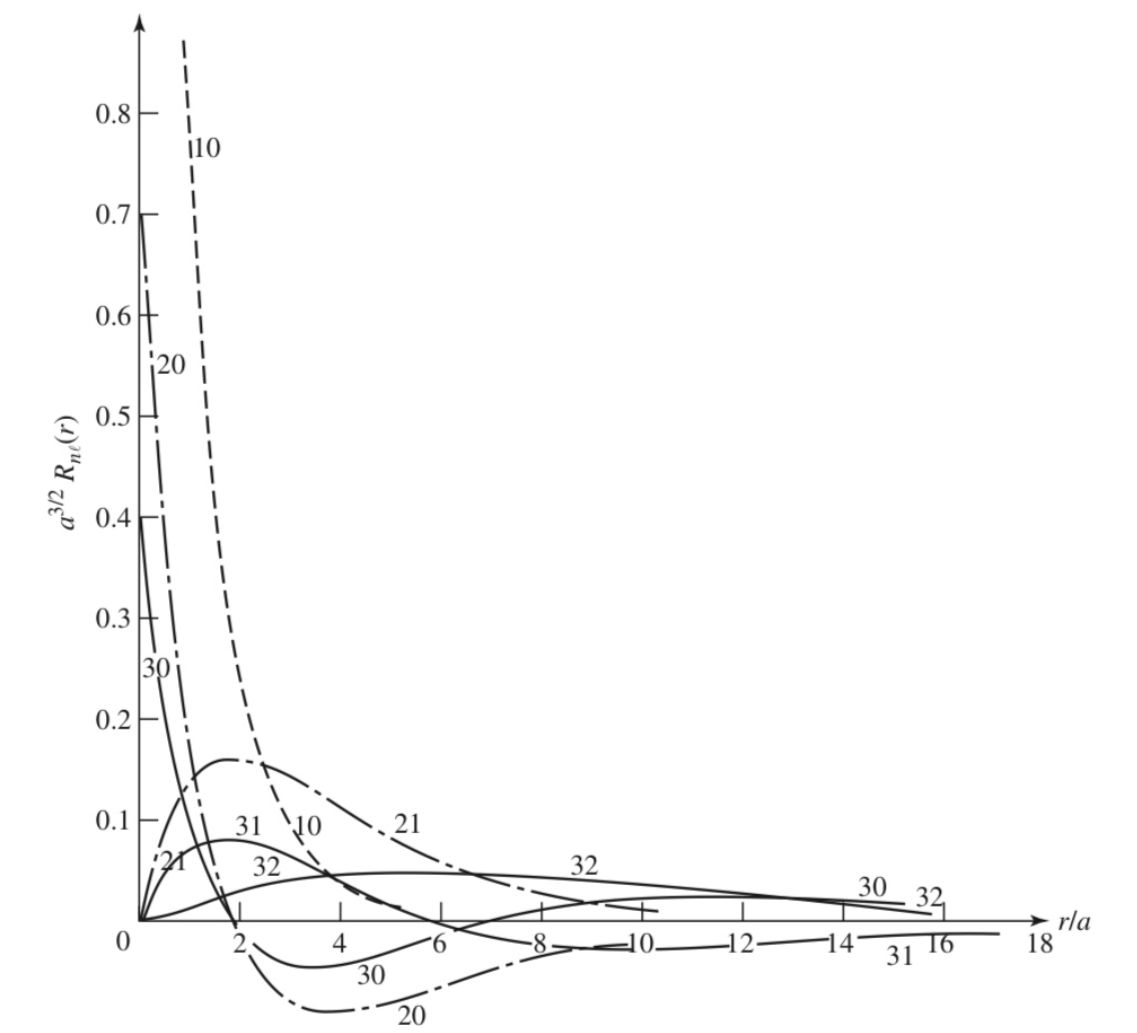
\includegraphics[width = 0.7 \textwidth]{chapter5/section3/imm/imm1.jpg}
\end{figure}

	Un modo invece di visualizzare l'intera funzione d'onda consiste nelle \textit{nubi di densità} in cui la luminosità della nube è proporzionale a $|\psi|^2$:

\begin{figure}[H]
  	\centering
	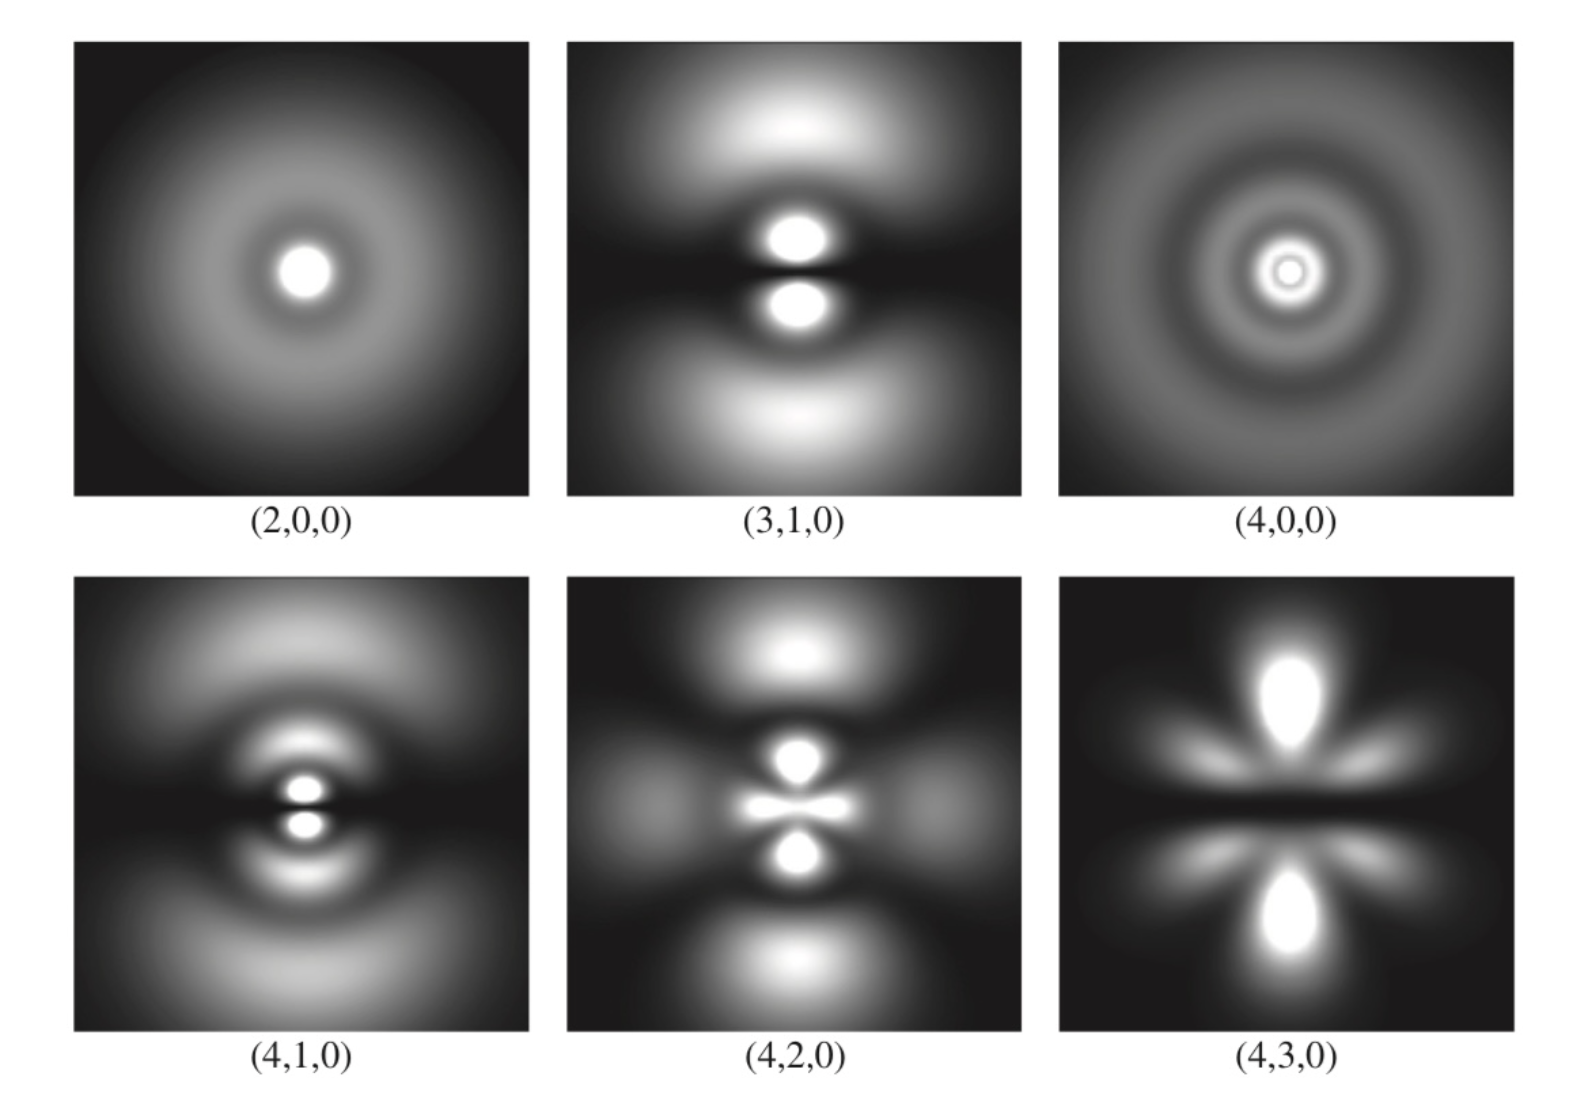
\includegraphics[width = 0.75 \textwidth]{chapter5/section3/imm/imm2.jpg}
\end{figure}

	mentre un modo alternativo più quantitativo ma più difficile da visualizzare, consiste nelle \textit{superfici con densità di probabilità costante}, ovvero:
	
\begin{figure}[H]
  	\centering
	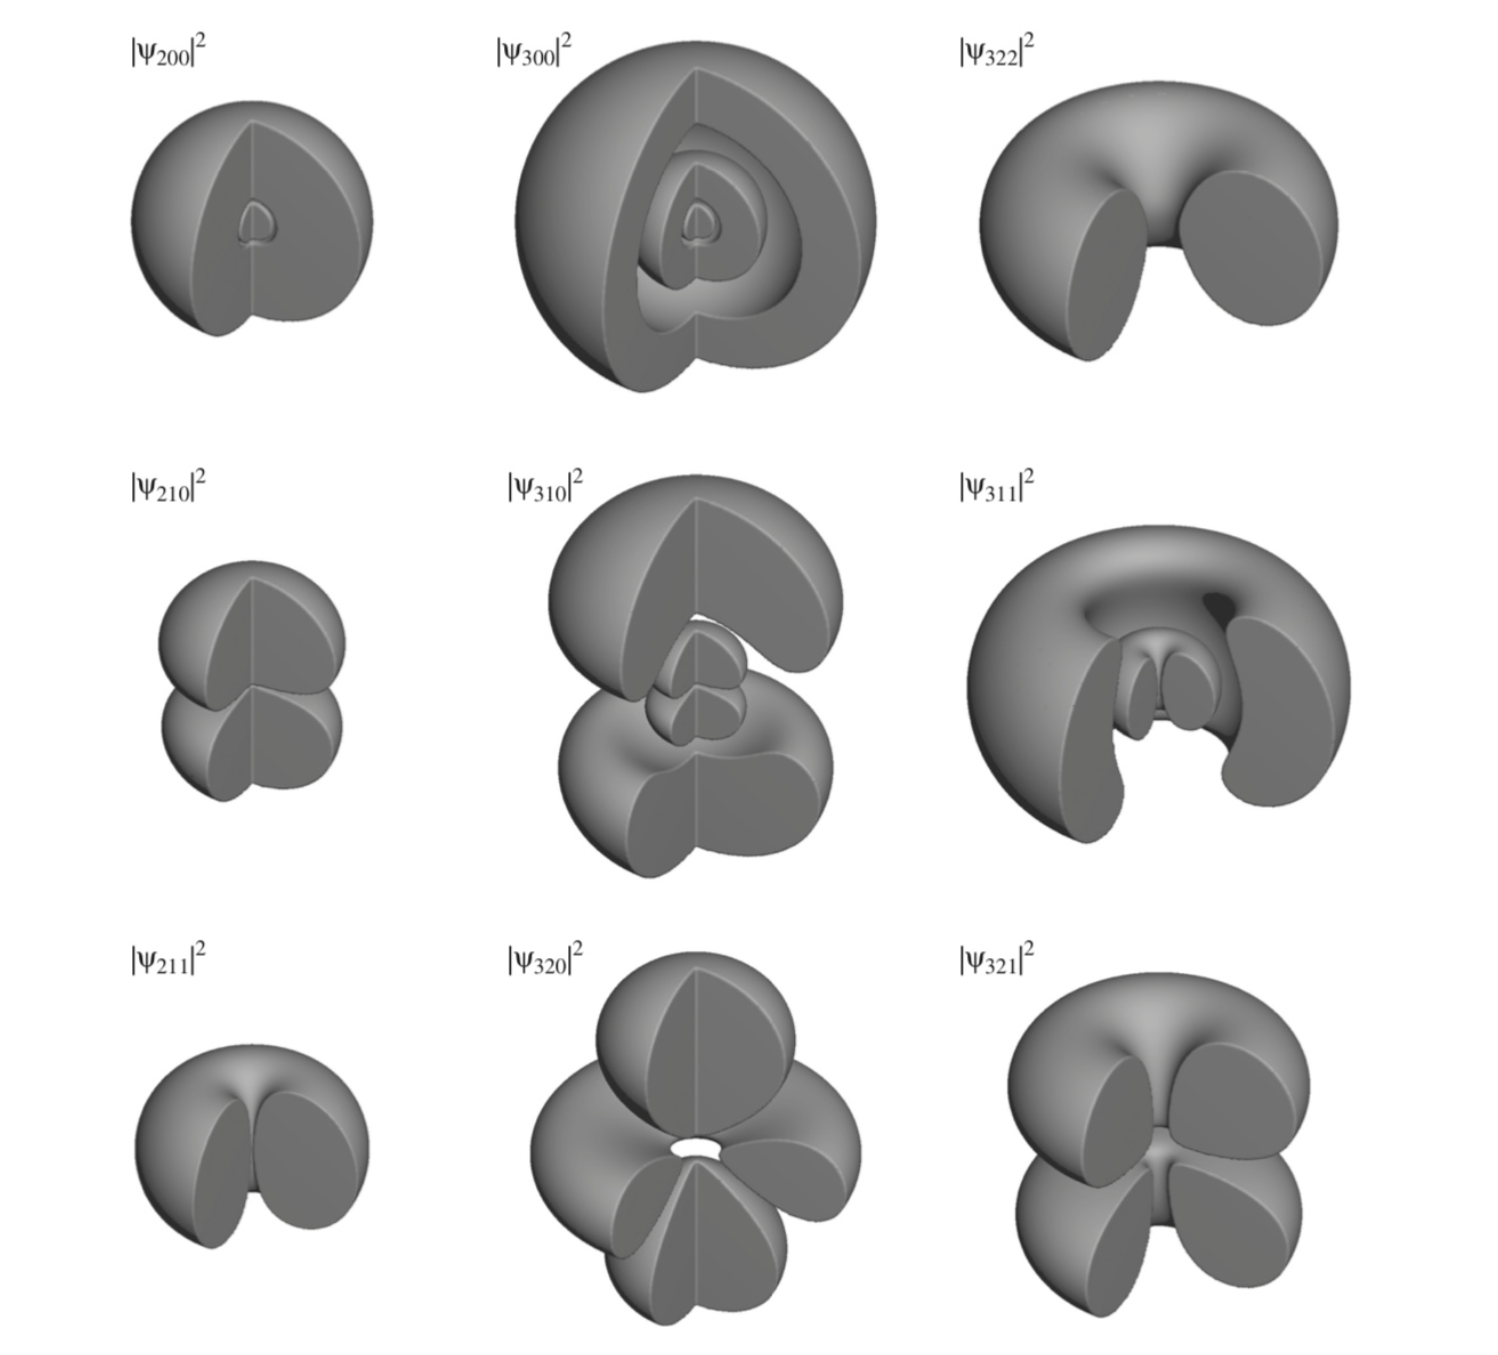
\includegraphics[width = 0.86 \textwidth]{chapter5/section3/imm/imm3.jpg}
\end{figure}

	Per concludere il discorso sull'atomo di Idrogeno facciamo un'ultima considerazione: come teniamo conto del fatto che l'elettrone ha uno spin?
	\\
	\\
	Se l'Hamiltoniana non dipende esplicitamente dallo spin allora una generica funzione d'onda, nella base degli autostati:
	
\begin{align*}
	\ket{n \, l \, m \, \sigma}
\end{align*}

	con $\sigma$ che indica la proiezione dello spin sull'asse $z$, sarà espressa come il prodotto tra la funzione d'onda orbitale $\psi_{nlm}$ ed una combinazione lineare dei vettori della base dello spin $1/2$, $\qty{\ket{+} \, \ket{-}}$, ossia:
	
\begin{align*}
	\Psi_{nlm}\qty(r, \theta, \phi, \sigma) = \alpha \, \psi_{nlm} \qty(r, \theta, \phi) \ket{+} + \beta \, \psi_{nlm}\qty(r, \theta, \phi) \ket{-}
\end{align*}

	scritta anche come:
	
\begin{align*}
	\Psi_{nlm} \qty(r, \theta, \phi, \sigma) = \mqty( \alpha \, \psi_{nlm} \qty(r, \theta, \phi, +) \\  \beta \, \psi_{nlm} \qty(r, \theta, \phi, -) )
\end{align*}

	pertanto ogni stato dell'atomo di Idrogeno ha una degenerazione pari a $2n^2$: per ogni $n, l, m$ fissati ho una degenerazione spaziale $n^2$, a cui però va aggiunta la degenerazione di spin che è $2$, che deriva dalla possibilità di avere spin up oppure spin down. In modo del tutto simile, se considerassimo anche la presenza dello spin protonico, avremmo un ulteriore fattore $2$ di degenerazione di spin, portando la degenerazione complessiva ad essere $4n^2$.







%%%%%%%FILE 1%%%%%%

%%%%%%%QUIQUIQUIQUI%%%%%%
\chapter{Sistemi di Particelle Identiche}

	Si consideri un sistema composto del tipo $\mathcal{H}_1 \otimes \mathcal{H}_2$. Esso ha dimensione:
	
\begin{align*}
	\dim \mathcal{H} = n_1 n_2
\end{align*}

	che sono rispettivamente la dimensione di $\mathcal{H}_1$ e $\mathcal{H}_2$.
	\\	
	\\
	Mi metto nel caso in cui vale: $\mathcal{H}_1 = \mathcal{H}_2$, cioè nel caso in cui gli autospazi sono descritti dalle osservabili. Se ho una soluzione per $\mathcal{H}$, posso allora scambiare i pedici $1$ e $2$ ed avere di nuovo una soluzione per $\mathcal{H}$: si tratta di una \textit{simmetria di scambio.}
	\\
	\\
	In meccanica classica, date $2$ particelle ad esempio, se fisso le condizioni iniziali potrò sempre distinguere l'una dall'altra siccome soddisfano una legge del moto definita e seguono quindi delle traiettorie fisse nello spazio delle fasi. Invece, in meccanica quantistica, esistono \textbf{sistemi di particelle identiche}, ossia \textit{indistinguibili} dal momento che non esistono traiettorie. Non ho dunque modo di distinguere fisicamente la situazione $\qty(1, 2)$ o $\qty(2, 1)$. Si tratta del \textbf{principio di indistinguibilità}. Un esempio di sistema di particelle identiche è un sistema di due elettroni.

\section{Principio di Pauli: bosoni e fermioni}

	Generalizzando ad $N$ particelle, si abbiano $N$ autospazi di dimensione $k$, ovvero tali che:

\begin{align*}	
	\dim \mathcal{H}_k = k \, \, \Rightarrow \, \, \dim \mathcal{H}_N = \dim \qty(\mathcal{H}_k \otimes \ldots \otimes \mathcal{H}_k)
\end{align*}

	se siamo nel caso in cui tali sottospazi sono \textit{distinguibili}, allora:
	
\begin{align*}
	\dim \mathcal{H}_k = k^N
\end{align*}

	altrimenti devo togliere tutti i sottospazi identici ad altri. In altre parole, se una base di $\mathcal{H}_k$ è:
	
\begin{align*}
	\qty{ \ket{\alpha}, \, \alpha = 1, \ldots, k}
\end{align*}

	una base di $\mathcal{H}_N$ sarà:
	
\begin{align*}
	\qty{\ket{\alpha_1}, \ldots, \ket{\alpha_N}, \, \alpha_i = 1, \ldots, k}
\end{align*}
	
	quindi ad esempio se non distinguo $\ket{\alpha_1}\ket{\alpha_2}$ da $\ket{\alpha_2} \ket{\alpha_1}$, dovrò tenere conto della presenza di questi due stati indistinguibili. Introduco allora il seguente operatore:
	
\begin{mydef}	
	Definiamo l'\textbf{operatore di scambio} $\hat{P}$, ossia una matrice le cui entrate sono:
	
\begin{align*}
	\hat{P}_{ij} : \mathcal{H}_N \to \mathcal{H}_N
\end{align*}

	tale che:
	
\begin{align*}
	\ket{\alpha_1} \cdots \ket{\alpha_i} \cdots \ket{\alpha_j} \cdots \ket{\alpha_N} \to \ket{\alpha_1} \cdots \ket{\alpha_j} \cdots \ket{\alpha_i} \cdots \ket{\alpha_N}
\end{align*}

	e che è unitaria. Pertanto vale:

\begin{align*}
	\hat{P}_{ij}^2 = \mathbb{I} \qquad ; \qquad \hat{P}_{ij}^{\dagger} = \hat{P}_{ij}
\end{align*}

\end{mydef}

	Enunciamo ora il seguente ed importantissimo principio, il \textbf{principio di Pauli}:
	
\begin{myprinc}

	Il \textbf{principio di Pauli} si articola nei seguenti $3$ punti:

\begin{enumerate}[label=\arabic*)]

	\item In un sistema di particelle identiche, le \textbf{osservabili fisiche} sono una sottoalgebra del sistema complessivo: tutte le \textit{osservabili fisiche} sono quelle in cui operatori associati commutano con $\hat{P}_{ij}$:
	\begin{align*}
		\hat{O} : \mathcal{H}_N \to \mathcal{H}_N \, \, \Rightarrow \, \, \qty[\hat{O}, \hat{P}_{ij}] = 0
	\end{align*}

	\item Come agisce $\hat{P}_{ij}$ sullo stato $\psi$? 
	
		Ho che:
	
	\begin{align*}
		\hat{P}_{ij} \psi = \lambda \psi \, \, \Rightarrow \, \, \hat{P}_{ij}^2 \psi = \lambda \hat{P}_{ij} \psi \, \, \Rightarrow \, \, \hat{P}^2_{ij} \psi = \lambda^2 \psi 
	\end{align*}
	
		ed essendo che $\hat{P}^2_{ij} = \mathbb{I}$ per ipotesi allora:
		
	\begin{align*}
		\psi = \lambda^2 \psi  \, \, \Rightarrow \, \, \lambda = \pm 1
	\end{align*}

		pertanto, poiché dal primo punto so che $\mathcal{H}_{\text{fisici}} \subset \mathcal{H}$, in particolare ho che la sottoalgebra è composta da stati simmetrici e stati antisimmetrici:
		
	\begin{align*}
		& \mathcal{H}_+ = \qty{\psi \in \mathcal{H}_N, \, \hat{P}_{ij}\psi = \psi, \, \forall i, j } \, \, \Rightarrow \, \, \textbf{simmetrici} \\
		& \mathcal{H}_- = \qty{\psi \in \mathcal{H}_N, \, \hat{P}_{ij}\psi = - \psi, \, \forall i, j } \, \, \Rightarrow \, \, \textbf{antisimmetrici}
	\end{align*}
	
	\item Quando $\mathcal{H}_k$ è lo spazio degli stati di una particella non relativistica che si muove in uno spazio tridimensionale con spin $s$, cioè quando:
	
	\begin{align*}
		\mathcal{H}_k = L_2\qty(\mathbb{R}^3) \otimes \mathcal{H}_s	
	\end{align*}
		
		si ha allora:
	
	\begin{itemize}
		\item $\mathcal{H}_k = \mathcal{H}_{+}$ se $s$ è \textbf{intero}: in questo caso la particella segue la \textit{statistica di Bose-Einstein}, per questo si parla di \textbf{bosoni}. La dimensione dello spazio è:
		\begin{align*}
			\dim \mathcal{H}_+ = \mqty(N + k -1 \\ k -1)
		\end{align*}
		
		\item $\mathcal{H}_k = \mathcal{H}_{-}$ se $s$ è \textbf{semintero}: in questo caso invece la particella segue la \textit{statistica di Fermi-Dirac}, per questo si parla di \textbf{fermioni}. La dimensione dello spazio è:
		\begin{align*}
			\dim \mathcal{H}_- = \mqty(k \\ N) \quad \text{se} \, \, \, N \leq k
		\end{align*}
			altrimenti se $ N \geq k$, la dimensione è nulla.
	\end{itemize}
	
	tutto ciò va sotto al nome: \textbf{Connessione Spin - Statistica} che in meccanica quantistica non relativistica è un assioma, mentre in meccanica quantistica relativistica è un teorema vero e proprio.

\end{enumerate}
\end{myprinc}

	Consideriamo ora anche lo spin. 
	\\
	\\
	Ad esempio, per $N = 2$, nel caso dei bosoni si ha che:
	
\begin{align*}
	\Psi_+ \qty(\vb{r}_1, \vb{r}_2, \sigma_1, \sigma_2) = \frac{1}{\sqrt{2}} \, \qty\Big( \psi_a\qty(\vb{r}_1, \sigma_1) \, \psi_b\qty(\vb{r}_2, \sigma_2) + \,  \psi_a\qty(\vb{r}_2, \sigma_2) \, \psi_b \qty(\vb{r}_1, \sigma_1)     )
\end{align*}

	mentre nel caso di fermioni:

\begin{align*}
	\Psi_- \qty(\vb{r}_1, \vb{r}_2, \sigma_1, \sigma_2) = \frac{1}{\sqrt{2}} \, \qty\Big( \psi_a\qty(\vb{r}_1, \sigma_1) \, \psi_b\qty(\vb{r}_2, \sigma_2) - \,  \psi_a\qty(\vb{r}_2, \sigma_2) \, \psi_b \qty(\vb{r}_1, \sigma_1)     )
\end{align*}

	dove $a$ e $b$ etichettano le due particelle: dal principio di indistinguibilità non posso sapere chi è uno e chi sia l'altro, pertanto la funzione d'onda sarà una combinazione lineare dei due possibili casi (particella $a$ in $\qty(\vb{r}_1, \sigma_1)$ e particella $b$ in $\qty(\vb{r}_2, \sigma_2)$ e viceversa), la cui simmetria sarà dettata dall'algebra del sottospazio fisico a cui appartengono (pari per i bosoni e dispari per i fermioni). 
	\\
	\\
	Da ciò deriva il più noto, anche se è conseguenza diretta del principio generale, \textbf{principio di esclusione}:
	
\begin{myprinc}
	\textit{Due fermioni identici non possono occupare simultaneamente lo stesso stato.}
\end{myprinc}

	La simmetria della funzione d'onda è dettata dall'algebra del sottospazio a cui le particelle appartengono: per i fermioni, la funzione d'onda deve essere dispari (antisimmetrica) rispetto allo scambio di due particelle. Questo significa che se scambi due fermioni identici, la funzione d'onda cambia segno:
	
\begin{align*}
	\Psi\qty(2, 1) = - \Psi\qty(1, 2)
\end{align*}

	Per soddisfare questa proprietà antisimmetrica, la funzione d'onda totale $\Psi_-$ si costruisce sottraendo le due possibili configurazioni:
	
\begin{align*}
	\Psi_- \sim \psi_a\qty(1)\psi_b\qty(2) - \psi_a\qty(2)\psi_b\qty(1)
\end{align*}

	 Se facessimo finta che non valga il \textit{principio di Pauli}, potremmo avere che nell'esempio di prima $\Psi_-\qty(\vb{r}_1, \vb{r}_2) = 0$, poiché ho il termine $\psi_a\qty(\vb{r}_1, \sigma_1) \psi_b\qty(\vb{r}_1, \sigma_1)$ meno se stesso, che è impossibile. Infatti se la funzione d'onda $\Psi$ è identicamente zero, significa che la probabilità di trovare il sistema in quella configurazione è nulla (la particella non esiste). Quindi, fisicamente, quello stato non può realizzarsi.
	\\
	\\
	In generale, per $n$ particelle identiche, posso fattorizzare la funzione d'onda in una parte spaziale ed una di spin (\textbf{spinore}):
	
\begin{align*}
	\Psi\qty(\vb{r}_1, \ldots, \vb{r}_n, \sigma_1, \ldots, \sigma_n) = \phi\qty(\vb{r}_1, \ldots, \vb{r}_n) \, \chi\qty(\sigma_1, \ldots, \sigma_n)
\end{align*}

	Prendiamo per esempio il caso di $n  = 2$ fermioni identici. Poiché l'operatore di scambio agisce simultaneamente sulle due funzioni, per garantire l'antisimmetria complessiva della funzione, ho che:

\begin{itemize}
	\item Se la parte spaziale è simmetrica, la parte di spin deve essere antisimmetrica allora:
	\begin{align*}
		\psi\qty(\vb{r}_1, \vb{r}_2) = \psi\qty(\vb{r}_2, \vb{r}_1) \qquad ; \qquad \chi\qty(\sigma_1, \sigma_2) = - \chi\qty(\sigma_2, \sigma_1)
	\end{align*}

	\item Se la parte spaziale invece è antisimmetrica, la parte di spin deve essere simmetrica:
	\begin{align*}
		\psi\qty(\vb{r}_1, \vb{r}_2) = - \psi\qty(\vb{r}_2, \vb{r}_1) \qquad ; \qquad \chi\qty(\sigma_1, \sigma_2) = \chi\qty(\sigma_2, \sigma_1)
	\end{align*}
	
\end{itemize}
		
	Discorso analogo vale per $n = 2$ bosoni identici. Poiché l'operatore di scambio agisce simultaneamente sulle due funzioni, per garantire la simmetria complessiva della funzione ho che:
	
\begin{itemize}
	
	\item Se la parte spaziale è simmetrica, la parte di spin deve essere simmetrica:
	\begin{align*}
		\psi\qty(\vb{r}_1, \vb{r}_2) =  \psi\qty(\vb{r}_2, \vb{r}_1) \qquad ; \qquad \chi\qty(\sigma_1, \sigma_2) = \chi\qty(\sigma_2, \sigma_1)
	\end{align*}
	
	\item Se la parte spaziale è antisimmetrica, la parte di spin deve essere antisimmetrica:
	\begin{align*}
		\psi\qty(\vb{r}_1, \vb{r}_2) =  -\psi\qty(\vb{r}_2, \vb{r}_1) \qquad ; \qquad \chi\qty(\sigma_1, \sigma_2) = -\chi\qty(\sigma_2, \sigma_1)
	\end{align*}
	
\end{itemize}

	Prima di andare avanti, è opportuno fare alcune considerazioni molto delicate, che avranno però importanti conseguenze. 
	\\
	\\
	Consideriamo due particelle in moto in un potenziale centrale, che dipende soltanto dalla distanza relativa tra di esse. L'Hamiltoniana che descrive il sistema è:
	
\begin{align*}
	\hat{H} = \frac{\hat{\vb{p}}^2_1}{2m_1} + \frac{\hat{\vb{p}}^2_2}{2m_2} + V\qty(r)
\end{align*}

	dove $r = |\vb{r}_1 - \vb{r}_2|$ è la coordinata relativa tra le due particelle. Definisco ora la coordinata del \textit{centro di massa} come:
	
\begin{align*}
	\vb{R}_{\text{CM}} = \frac{m_1 \vb{r}_1 + m_2 \vb{r}_2}{m_1 + m_2}
\end{align*}

	da cui ho:
	
\begin{align*}
	\vb{V}_{\text{CM}} = \frac{m_1 \vb{v}_1 + m_2 \vb{v}_2}{m_1 + m_2}
\end{align*}

	e allora posso scrivere la quantità di moto rispetto al centro di massa come:
	
\begin{align*}
	\vb{P}_{\text{CM}} = \qty(m_1 + m_2) \, \vb{V}_{\text{CM}} = \vb{p}_1 + \vb{p}_2
\end{align*}

	Ricordiamo ora del problema a due corpi, le singole quantità di moto sono espresse in termini di quantità di moto relativa, ovvero:
	
\begin{align*}
	\vb{p}_{\text{rel}} = \mu \, \vb{V}_{\text{rel}}
\end{align*}

	dove $\mu$ è la \textit{massa ridotta} e allora possiamo scrivere:

\begin{align*}
	\vb{p}_{\text{rel}} = \mu \, \vb{V}_{\text{rel}} = \frac{m_1 m_2}{m_1 + m_2} \, \vb{V}_{\text{rel}} = \frac{m_1 m_2}{m_1 + m_2} \, |\vb{v}_1 - \vb{v}_2| = \frac{m_2 \vb{p}_1 - m_1 \vb{p}_2}{ m_1 + m_2 } 
\end{align*}

	dove infatti:
	
\begin{align*}
	& \vb{p}_1 = m_1 \vb{v}_1 \, \Rightarrow \, \vb{v}_1 = \frac{\vb{p}_1}{m_1} \\
	& \vb{p}_2 = m_2 \vb{v}_2 \, \Rightarrow \, \vb{v}_2 = \frac{\vb{p}_2}{m_2}
\end{align*}

	allora possiamo trovare:
	
\begin{align*}
	\vb{p}_1 = \frac{m_1}{m_1 + m_2} \, \vb{P}_{\text{CM}} + \vb{p}_{\text{rel}} \qquad ; \qquad \vb{p}_2 = \frac{m_2}{m_1 + m_2} \, \vb{P}_{\text{CM}} - \vb{p}_{\text{rel}}
\end{align*}

	Se adesso si vanno a sostituire i due termini nell'Hamiltoniana di partenza, si trova che:
	
\begin{align*}
	\hat{H} = \frac{\vb*{\hat{P}}^2_{\text{CM}} }{2M} + \frac{\vb*{\hat{p}}^2_{\text{rel}} }{2\mu} + V\qty(r)
\end{align*}

	Questa è l'Hamiltoniana \textit{separata} nelle coordinate del centro di massa e relative. La prima parte:
	
\begin{align*}
	\frac{\vb*{\hat{P}}^2_{\text{CM}}}{2M}
\end{align*}

	descrive il moto del centro di massa, mentre la seconda parte:
	
\begin{align*}
	\frac{\vb*{\hat{p}}^2_{\text{rel}}}{2\mu} + V\qty(r)
\end{align*}
	
	descrive il moto relativo delle due particelle nel potenziale scelto.
	\\
	\\
	Che conseguenze ha tutto ciò?
	\\
	\\
	L'aver separato la coordinata relativa da quella del centro di massa permette di fattorizzare la funzione d'onda spaziale come:
	
\begin{align*}
	\Phi\qty(\vb{R}, \vb{r}) = \phi_{\text{CM}}\qty(R) \, \phi_{\text{rel}}\qty(r)
\end{align*}
	
	dove la funzione d'onda spaziale relativa è formalmente identica alla funzione d'onda dell'atomo di Idrogeno, perciò è possibile scrivere:
	
\begin{align*}
	\phi_{\text{rel}}\qty(r) = R_{nl}\qty(r) \, Y_l^m\qty(\theta, \phi)
\end{align*}
	
	Consideriamo adesso il caso di \textbf{particelle identiche}: cosa succede se applico la simmetria di scambio alla funzione d'onda?
	\\
	\\
	La parte dipendente dal centro di massa non subirà cambiamenti, ma la parte dipendente dalla coordinata relativa si. Infatti per scambio da $1$ a $2$ e viceversa, ho che: $r = \vb{r}_1 - \vb{r}_2 \to \vb{r}_2 - \vb{r}_1 = -r$, che non apporta cambiamenti alla funzione, e $\qty(\theta, \phi) \to \qty(\pi - \theta, \phi + \pi)$ che invece secondo la parità delle armoniche sferiche sotto inversione spaziale:
	
\begin{align*}
	\Pi Y_l^m \qty(\theta, \phi) = Y_l^m \qty(\pi - \theta, \phi + \pi) = \qty(-1)^l \, Y_l^m\qty(\theta, \phi)
\end{align*}
	
	che si porta dietro un fattore $\qty(-1)^l$, che determina in conclusione la \textbf{simmetria della funzione d'onda spaziale}.
	\\
	\\
	Si consideri un elettrone (\textit{fermione}) e si indichi con $\hat{H}^{\qty(1)}$ il suo spazio di singola particella. Lo spazio $\hat{H}^{\qty(1)}$ è un prodotto tensore tra il suo spazio orbitale ed il suo spazio di spin, ovvero:
	
\begin{align*}
	\hat{H}^{\qty(1)} = \mathcal{H}_{\text{orb}} \otimes \mathcal{H}_s
\end{align*}

	Sia $\qty{\ket{n}, \, n = 0, 1, 2, \ldots }$ una base discreta dell'autospazio $\mathcal{H}_{\text{orb}}$. Si abbiamo ora $N = 2$ elettroni, di cui consideriamo solo lo spin. 
	\\
	\\
	Quanti sono gli stati del sistema di due fermioni $\mathcal{H}^{\qty(1)} \otimes \mathcal{H}^{\qty(1)}$?
	\\
	\\
	Per rispondere a questa domanda dobbiamo conoscere la dimensione dello spazio orbitale: in genere essa è infinita, poiché i numeri quantici possono assumere infiniti valori, tuttavia scelgo di studiare cosa succede a $2$ elettroni su $2$ livelli energetici. Ovvero scelgo: $\dim \mathcal{H}_{\text{orb}} = 2$. Che dimensione ha lo spazio fermionico associato a $\mathcal{H}_-$? Poiché:
	
\begin{align*}
	\dim \mathcal{H}^{\qty(1)} = \dim \mathcal{H}_{\text{orb}} \cdot \dim \mathcal{H}_{s} = 2 \, \qty(2 s + 1) \, \equiv \, k
\end{align*}

	si ha, per $N = 2$ (prendiamo infatti in esame $2$ elettroni) che vale :
	
\begin{align*}
	\dim \mathcal{H}_- = \mqty(k \\ N) = \mqty(2\qty(2s + 1) \\ 2) 
\end{align*}

	ricordando che:
	
\begin{align*}
	\mqty(k \\ N) = \frac{k!}{N!\, \qty(k - N)!} 
\end{align*}

	allora:

\begin{align*}
	 \mqty(2\qty(2s + 1) \\ 2)  = \qty(2s + 1)\, \qty(4s + 1)
\end{align*}

	Adesso \textit{costruisco due operatori che commutano con $\hat{P}$, l'\textcolor{cyan}{energia totale del sistema} e lo \textcolor{orange}{spin totale del sistema}:}
	
\begin{align*}
	& \textcolor{cyan}{\hat{H} } = \hat{H}^{\qty(1)} \otimes \mathbb{I} + \mathbb{I} \otimes \hat{H}^{\qty(1)} \\
	& \textcolor{orange}{ \hat{S}_z }= \hat{S}_z^{\qty(1)} \otimes \mathbb{I} + \mathbb{I} \otimes \hat{S}_z^{\qty(1)}
\end{align*}

	tali che, detta la base di $\mathcal{H}_N = \mathcal{H}^{\qty(1)} \otimes \mathcal{H}^{\qty(1)}$ la seguente:
	
\begin{align*}
	\qty{ \ket{n_1}\ket{\sigma_1}, \, \ket{n_2} \ket{\sigma_2} ; \, n_i = 1, 2 \, ;  \, \sigma = -s, \ldots, + s  }
\end{align*}

	allora si ha:
	
\begin{align*}
	& \hat{H}\ket{n_1, \sigma_1; \, n_2, \sigma_2} = \qty(E_{n_1} + E_{n_2}) \ket{n_1, \sigma_1; \, n_2, \sigma_2} \\
	& \hat{S}_z\ket{n_1, \sigma_1; \, n_2, \sigma_2} = \qty(\sigma_{n_1} + \sigma_{n_2}) \ket{n_1, \sigma_1; \, n_2, \sigma_2}
\end{align*}

	quindi uno stato del sistema composto è assegnato se ho $n_1, n_2$ e $\sigma_1, \sigma_2$. In generale ho $3$ livelli energetici distinti: per un generico valore di $s$, come si distribuiscono quindi i $\qty(2s + 1) \qty(4s + 1)$ stati sui vali livelli?


\begin{itemize}
	\item $E = 2 E_1$
		
		Entrambi gli elettroni sono sul livello $E_1$. Ho quindi $n_1 = n_2 = 1$, quindi una base è $\qty{\ket{1, \sigma_1}, \ket{1, \sigma_2}}$. Questo significa che entrambi gli elettroni si trovano sul livello energetico fondamentale $E_1$ (quindi $n_1=1$ e $n_2=1$). La parte spaziale della funzione d'onda è quindi il prodotto dello stato $1$ con se stesso:
		
	\begin{align*}
		\psi_{\text{spazio}} = \ket{1}\ket{1}
	\end{align*}
	
		se scambi le due particelle ottieni ancora $\ket{1}\ket{1}$, quindi la parte spaziale è \textit{simmetrica}. I fermioni devono avere una funzione d'onda totale \textit{antisimmetrica} (devono cambiare segno se li scambi).
La funzione totale è il prodotto di Spazio $\times$ Spin. Ossia:

	\begin{align*}
		\Psi_{\text{tot}} = \psi_{\text{spazio}} \otimes \chi_{\text{spin}}
	\end{align*}

		Affinché il totale sia antisimmetrico, poiché sistema di fermioni, dato che lo spazio è simmetrico, la parte di spin deve essere obbligatoriamente \textit{antisimmetrica}. La funzione d'onda relativa a questa configurazione energetica è allora:
	
	\begin{align*}
		\Psi_{\sigma_1, \sigma_2}^{\qty(2E_1)} = \frac{1}{\sqrt{2}} \, \qty(\ket{1, \sigma_1} \ket{1, \sigma_2} - \ket{1, \sigma_2} \ket{1, \sigma_1})
	\end{align*}
	
		quanti sono questi stati?
		\\
		\\
		Ora il problema diventa puramente combinatorio: quanti stati di spin antisimmetrici esistono per due particelle con spin $s$?
		\\
		\\
		Il numero di spin per una singola particella: $N_s = 2s + 1$ e dobbiamo scegliere $2$ stati di spin diversi ($\sigma_1 \neq \sigma_2$) tra gli $N_s$ disponibili per formare una combinazione antisimmetrica del tipo $(\sigma_1 \sigma_2 - \sigma_2 \sigma_1)$. Non possono essere uguali altrimenti la differenza fa zero (Principio di Pauli), allora vale la formula?
		
	\begin{align*}
		\text{numero di conteggi} & = \mqty(2s + 1 \\ 2) = \frac{\qty(2s + 1)!}{2! \, \qty(\qty(2s + 1) - 2)!} = \frac{\qty(2s + 1) \qty(2s) \qty(2s - 1)!}{ 2! \qty( 2s - 1)!} \\
		& = \frac{\qty(2s + 1) \qty(2s)}{2} = s  \qty(2 s + 1)
	\end{align*}
	
		Ho quindi $s \qty(2s + 1)$ stati possibili su questo livello energetico.
	
	\begin{myapprf}
		\textbf{Esempio:}
		\\
		\\
		Per 2 fermioni identici, per esempio $2$ elettroni, otteniamo: $s = 1/2$. Allora abbiamo:
		\begin{align*}
			s\qty(2s + 1) = 1
		\end{align*}
		È corretto? Sì. Se due elettroni sono nello stesso orbitale spaziale (simmetrico), devono essere nel singoletto di spin (antisimmetrico):
		\begin{align*}
			\frac{1}{\sqrt{2}} \, \qty(\ket{+} \ket{-} - \ket{-} \ket{+})
		\end{align*}
		C'è un solo stato possibile. Se provassero a stare in uno stato di spin simmetrico (i 3 stati del tripletto), la funzione totale diventerebbe simmetrica, il che è vietato per i fermioni (Pauli).

	\end{myapprf}
		
	\item $E = E_1 + E_2$
	
		Un elettrone è sul livello $E_1$ mentre l'altro elettrone è sul livello $E_2$. Quindi in questo caso abbiamo un elettrone sul livello energetico fondamentale $E_1$ (chiamiamolo stato orbitale 1) e l'altro sul livello eccitato $E_2$ (stato orbitale 2).
Poiché le energie sono diverse, le due particelle occupano zone spaziali diverse (o meglio, orbitali diversi).
	\\
	\\
		\textit{Il Principio di Esclusione di Pauli dice che due fermioni non possono avere tutti i numeri quantici uguali.} Nel caso precedente ($E=2E_1$), entrambi erano nello spaziale $1$, quindi dovevano avere spin diversi per non essere identici. In questo caso, invece, i fermioni sono già distinti dalla loro posizione (uno è in $1$, l'altro è in $2$).
	\begin{itemize}
		\item L'elettrone sul livello $1$ ha numeri quantici $(n=1, \sigma_1)$.
		\item L'elettrone sul livello $2$ ha numeri quantici $(n=2, \sigma_2)$.
	\end{itemize}
	
		Dato che $n=1$ è diverso da $n=2$, i due stati completi sono sempre diversi, indipendentemente dallo spin!
Anche se gli spin fossero identici ($\sigma_1 = \sigma_2$), le particelle non sarebbero nello stesso stato perché una è al "piano terra" e l'altra al "primo piano". Poiché non c'è nessun vincolo che lega lo spin del primo a quello del secondo, abbiamo la massima libertà di scelta:
	\begin{itemize}
		\item Scelta per l'elettrone su $E_1$: Può avere qualsiasi orientazione di spin. Quante opzioni ci sono? $2s+1$.
		\item Scelta per l'elettrone su $E_2$: Può avere, indipendentemente dall'altro, qualsiasi spin. Quante opzioni ci sono? $2s+1$.
	\end{itemize}
	
		Il numero totale di combinazioni è semplicemente il prodotto delle possibilità:
	\begin{align*}
		\text{numero di conteggi} = \qty(2s + 1)\qty(2s + 1) = \qty(2s + 1)^2
	\end{align*}
	
		La funzione d'onda infine è:
	\begin{align*}
		\Psi_{\sigma_1, \sigma_2}^{\qty(E_1 + E_2)} = \frac{1}{\sqrt{2}} \, \qty(\ket{1, \sigma_1} \ket{2, \sigma_2} - \ket{2, \sigma_2} \ket{1, \sigma_1})
	\end{align*}
	
		Questa formula costruisce automaticamente uno stato antisimmetrico valido per qualsiasi coppia di valori $\sigma_1$ e $\sigma_2$, proprio perché i ket $\ket{1}$ e $\ket{2}$ sono diversi.

	\item $E = 2 E_2$
	\\
	\\
		Entrambi gli elettroni sono sul livello $E_2$. In maniera del tutto analoga al primo caso allora si ottiene che la funzione totale è:
		
	\begin{align*}
		\Psi_{\sigma_1, \sigma_2}^{\qty(2E_2)} = \frac{1}{\sqrt{2}} \, \qty(\ket{2, \sigma_1} \ket{2, \sigma_2} - \ket{2, \sigma_2} \ket{2, \sigma_1})
	\end{align*}
	
		ed ho come il primo caso il numero di stati pari a:
		
	\begin{align*}
		\text{numero di conteggi} = s \qty(2s +1 )
	\end{align*}
	
\end{itemize}

	La somma delle tre degenerazioni è:
	
\begin{align*}
	2s \qty(2s + 1) + \qty(2s + 1)^2 = \qty(2s + 1) \qty(2s + 2s +1 ) = \qty(2s + 1) \qty(4s +1) = \text{dim} \, \mathcal{H}_-
\end{align*}

	Vediamo ora molto brevemente le due statistiche citate prima. Esse costituiscono un "aggiornamento" quantistico della statistica classica di Maxwell-Boltzmann.
	
\subsection{Statistica di Bose-Einstein}

	In questo caso in un qualsiasi stato può stare un numero arbitrario di particelle. Il numero medio di particelle che occupano lo stato $k$ è dato dalla statistica di Bose-Einstein e vale:
	
\begin{align*}
	\mean{n_k} = \frac{1}{e^{\qty(\varepsilon_k - \mu)/k_B T} - 1}
\end{align*}
	
	con energia media che vale:
	
\begin{align*}
	\mean{E_k} = \mean{n_k} \varepsilon_k = \frac{\varepsilon_k}{e^{\qty(\varepsilon_k - \mu)/k_B T} - 1}
\end{align*}

	diove $\varepsilon_k$ è il $k-$esimo stato e $\mu$ è il potenziale chimico.

\subsection{Statistica di Fermi-Dirac}

	In questo la forma della funzione d'onda è:
	
\begin{align*}
	\Psi\qty(\vb{r}_1, \dots, \vb{r}_N, \sigma_1, \dots, \sigma_N) = \frac{1}{\sqrt{N!}} \sum_P \qty(-1)^p P\qty{\psi_1\qty(\vb{r}_1, \sigma_1), \dots, \psi_N\qty(\vb{r}_N, \sigma_N)}
\end{align*}

	dove la somma è estesa a tutte le permutazioni $P$ delle variabili e $p$ è la parità della permutazione. Il membro di destra dell’equazione equivale allo sviluppo del \textbf{determinante di Slater}. In cui $N$ è il numero dei fermioni nel sistema. Da ciò segue subito che se due funzioni $\psi_i$ e $\psi_j$ sono uguali fra loro, ci saranno due righe uguali nel determinante che quindi si annullerà. In un sistema di fermioni identici, come già detto, non posso assegnare la stessa $\psi$ a due fermioni. Il formalismo del determinante di Slater è valido per un sistema di fermioni non interagenti in un qualsiasi tipo di potenziale e per ogni livello energetico, a patto di fare attenzione alla sua impostazione. Il numero medio delle particelle che occupano lo stato $k$ è la statistica di Fermi-Dirac.

\begin{align*}
	\mean{n_k} = \frac{1}{e^{\qty(\varepsilon_k - \mu)/k_B T} + 1}
\end{align*}
	
	con energia media che vale:
	
\begin{align*}
	\mean{E_k} = \mean{n_k} \varepsilon_k = \frac{\varepsilon_k}{e^{\qty(\varepsilon_k - \mu)/k_B T} + 1}
\end{align*}

\section{Particelle Identiche nel Potenziale Coulombiano}

	In questa sezione vediamo degli esempi di sistemi di particelle identiche nel potenziale Coulombiano, studiandone a grandi linee il comportamento.
	
\subsection{L'Atomo di Elio non Interagente}

	Consideriamo un sistema composto da $2$ elettroni (si tratta di $2$ fermioni identici) che interagiscono con un nucleo $Z = 2$. L'Hamiltoniana del sistema è data da:
	
\begin{align*}
	\hat{H} =  \textcolor{blue}{ \frac{\vb*{\hat{p}}^2_1}{2m} - \frac{2e^2}{4\pi \varepsilon_0 r_1} } + \textcolor{ForestGreen}{ \frac{ \vb*{\hat{p}_2^2}}{2m} - \frac{2e^2}{4\pi \varepsilon_0 r_2} } + \textcolor{orange}{  \frac{e^2}{4\pi\varepsilon_0} \, \frac{1}{| \vb{r}_1 - \vb{r}_2 |} }  \, \equiv \, \textcolor{blue}{ \hat{H}_1 } +  \textcolor{ForestGreen}{ \hat{H}_2 } + \textcolor{orange}{\hat{H}_{12}}
\end{align*}	

	per il momento trascuriamo l'interazione fra i due elettroni e poniamo quindi:
	
\begin{align*}
	\hat{H} = \hat{H}_1 + \hat{H}_2
\end{align*}

	Voglio descriverne lo spettro tenendo conto del \textit{Principio di Pauli:} per fare ciò scrivo il sistema di singola particella tenendo conto anche dello spin.
	
\begin{itemize}
	\item \textbf{Livello Fondamentale} $\qty(n_1 = n_2 = 1)$
	
		Il livello fondamentale dell'elio è composto da due elettroni in $n = 1$. L'energia del livello, in unità di Bohr, è quindi:
	\begin{align*}
		E^{\qty(1, 1)} = E_1^{\qty(1)} + E_2^{\qty(1)}
	\end{align*}

		Il calcolo deriva dall'applicazione della formula sopra all'atomo di Elio, considerando l'approssimazione "non interagente".
	\\
	\\
		L'atomo è di Elio e quindi $Z = 2$ (due protoni nel nucleo). Entrambi gli elettroni sono nel livello più basso possibile, quindi $n_1 = 1$ e $n_2 = 1$. Allora possiamo usare la formula:
	\begin{align*}
		& E_1^{\qty(1)} = - \frac{Z^2}{n_1^2} = - 4 \\
		& E_2^{\qty(1)} = - \frac{Z^2}{n_2^2} = - 4
	\end{align*}

		e quindi:
	
	\begin{align*}
		E^{\qty(1, 1)} = E_1^{\qty(1)} +  E_2^{\qty(1)} = - 8
	\end{align*}
	
		dire che l'energia è $-8$ significa dire che l'energia totale dello stato fondamentale dell'Elio (senza repulsione tra elettroni) è pari a 8 volte l'energia di legame dell'atomo di Idrogeno ($8 \cdot 13.6 \, \text{eV} \approx 108.8 \, \text{eV}$).
		\\
		\\
		Per il principio di Pauli, poiché sto considerando due fermioni, lo stato del livello è descritto dalla funzione d'onda:
	\begin{align*}
		\Psi^{\qty(1, 1)} = \frac{1}{\sqrt{2}} \qty(\ket{1, 0, 0, +}_1 \ket{1, 0, 0, 0, -}_2 - \ket{1, 0, 0, -}_1 \ket{1, 0, 0, +}_2)
	\end{align*}
	
		ed è l'unico modo possibile. Da un semplice calcolo si trova allora che il momento angolare orbitale dello stato fondamentale è: $L = 0$. Essa infatti è diretta conseguenza della regola della \textit{somma dei momenti angolari}. Ecco i passaggi logici:
		
		\begin{enumerate}
			\item Siccome siamo nello stato fondamentale, vale che entrambi gli elettroni si trovano sul livello energetico più basso possibile in cui: $n_1 = 1$ e $n_2 = 1$. Il momento angolare orbitale $l$ può allora assumere solo valori interi da $0$, fino ad $n-1$. Poiché $n = 1$ allora l'unica scelta possibile per $l$ è $0$. Quindi ne segue che il primo elettrone ha momento angolare orbitale pari a $l_1 = 0$ mentre il secondo ha momento angolare orbitale pari a $l_2 = 0$.
		
			\item Per trovare $L$ dobbiamo fare la somma vettoriale dei momenti angolari, ossia:
			\begin{align*}
				\vb{L} = \vb{l}_1 + \vb{l}_2
			\end{align*}
			
				$L$ quindi può variare tra la differenza e la somma dei singoli moduli:
			\begin{align*}
				|l_1 - l_2| \leq L \leq l_1 + l_2
			\end{align*}
				
				separati di $1$, siccome $l_1 = l_2 = 0$ in questo caso, si ottiene che l'unica soluzione possibile è proprio:
			\begin{align*}
				L = 0
			\end{align*}

		\end{enumerate}

			Quindi $L = 0$ abbiamo detto, allora per garantire l'antisimmetria complessiva della funzione d'onda, gli elettroni saranno in singoletto di spin: con $S = 0$. Infatti:
		
		\begin{align*}
			\vb{\frac{1}{2}} \otimes \vb{\frac{1}{2}} = \vb{1} \oplus \vb {0}
		\end{align*}
		
			dove infatti il prodotto tensore indica che sto combinando due sistemi indipendenti con spin $1/2$. La somma diretta risultante indica che il risultato si scompone (si disaccoppia) in due sottospazi distinti e indipendenti. Tuttavia, in fisica dobbiamo scartare $S=1$ a causa del \textit{Principio di Pauli.} Questo perché siccome la parte spaziale è simmetrica per scambio di elettrone, la parte di spin deve essere antisimmetrica, la decomposizione ci dice che, per particelle identiche, il primo spazio di spin è simmetrico e poi seguono gli altri alternandosi, allora necessariamente scelgo solo $S=0$. Non perché $S=1$ non esista matematicamente, ma perché è proibito dalla configurazione spaziale in cui mi trovo. Se gli elettroni fossero in orbitali diversi (spazio antisimmetrico), allora avresti dovuto scegliere $S=1$. Ma stando "nella stessa stanza" (livello fondamentale), devono per forza avere spin opposti in configurazione di singoletto per non violare il principio di esclusione. Quindi, siccome sia $L$ che $S$ sono zero, allora lo stato fondamentale ha $\qty(L, S, J) = \qty(0, 0, 0)$, ricordando infatti che $J = L + S$.

	\item \textbf{Primo livello eccitato} $\qty(n_1 = 1, n_2 = 2)$
	
		Passiamo ora al primo livello eccitato, in cui un elettrone è in $n = 1$ mentre l'altro è in $n = 2$. L'energia in questo caso è:
		
	\begin{align*}
		E^{\qty(1, 2)} = E_1^{\qty(1)} + E_2^{\qty(2)}
	\end{align*}
	
		dove:
		
	\begin{align*}
		& E_1^{\qty(1)} = - \frac{Z^2}{n_1^2} = -\frac{4}{1} = - 4 \\
		& E_2^{\qty(2)} = - \frac{Z^2}{n_2^2} = - \frac{4}{4} = -1
	\end{align*}
	
		allora:
		
	\begin{align*}
		E^{\qty(1, 2)} = - 5
	\end{align*}

		la funzione d'onda che descrive il livello è invece:
		
	\begin{align*}
		\Psi^{\qty(1, 2)} = \frac{1}{\sqrt{2}} \, \qty(\ket{1, 0, 0, \sigma}_1 \ket{2, l', m', \sigma'}_2 - \ket{2, l', m', \sigma'}_1 \ket{1, 0, 0, \sigma}_2)
	\end{align*}

		con quindi: $ n = 1$, allora: $l = m = 0$, con $\sigma = - s, -s +1, \dots, + s$ e siccome $s = 1/2$, allora: $\sigma = -1/2, 1/2$, infatti per $s  =1/2 $, ho $2s +1$ stati, ossia in questo caso, $2$. Invece, per $ n' = 2$, $ l' = 0, 1$, $m' = 0$ per $l' = 0$ mentre $m' = -1, 0, 1$ per $l' = 1$, invece $\sigma' = -1/2, 1/2$ come prima.
		\\
		\\
		Questa funzione d'onda deve essere totalmente antisimmetrica per scambio da $1$ a $2$ e viceversa, ossia per $l', m', \sigma, \sigma'$, fissati la funzione deve essere antisimmetrica. 
		\\
		\\
		Qual è la degenerazione di questo livello? L'elettrone nello stato fondamentale ha degenerazione $2$ poiché ha solo una doppia degenerazione di spin, invece l'elettrone nel primo livello ha degenerazione $8$ poiché ha due possibili stati di spin e due possibili valori di $l'$ e quindi ha anche $4$ possibili valori di $m'$ ed in totale $8$, perciò la degenerazione totale del livello è $16$. In generale si può dire subito la degenerazione del livello tenendo conto che la degenerazione di un singolo livello è pari a $2n^2$. Più nello specifico, questi $16$ stati che $L$ e $S$ avranno?
		\\
		\\
		Si ha che:
	
	\begin{align*}
		l = 0, \,\,\, l' = 0, 1 \,\, \Rightarrow \,\, L = l \otimes l' = 0 \otimes \qty( 0 \oplus 1) = 0 \oplus 1 
	\end{align*}
		
		e vale che:

	\begin{align*}
		s = \frac{1}{2}, \,\,\, s' = \frac{1}{2} \,\, \Rightarrow \,\, S = s \otimes s' = \frac{1}{2} \otimes \frac{1}{2} = 0 \oplus 1 
	\end{align*}

		allora in questo caso, essendo su due livelli distinti gli elettroni non hanno restrizioni e non dobbiamo cancellare nessun valore. Le terne di $\qty(L, S, J)$ possibili sono:
		
	\begin{align*}
		\qty(L, S, J) & = \qty(0, 0, 0) \, \Rightarrow \, \text{deg} = 1 \\
		& = \qty(0, 1, 1) \, \Rightarrow \, \text{deg} = 3 \\
		& = \qty(1, 0, 1) \, \Rightarrow \, \text{deg} = 3 \\
		& = \qty(1, 1, 0) \, \Rightarrow \, \text{deg} = 1 \\
		& = \qty(1, 1, 1) \, \Rightarrow \, \text{deg} = 3 \\
		& = \qty(1, 1, 2) \, \Rightarrow \, \text{deg} = 5 \\
	\end{align*}
	
		le cui singole degenerazioni sono calcolate a partire da $2j + 1 $ applicato a $L$ e $S$, moltiplicate fra loro e sommate in totale, oppure al valore di $J$ e sommate in totale: si ritrova una \textit{degenerazione totale} di $16$. Lo spazio totale in cui vive $J$ è generato dal prodotto dello spazio di $L$ e dello spazio di $S$ e vale:
		
	\begin{align*}
		\mathcal{D}_L \otimes \mathcal{D}_S = \bigoplus_{J = |L - S|}^{L + S} \mathcal{D}_J
	\end{align*}

\end{itemize}

\subsection{L'atomo di Litio non Interagente}
	
	Consideriamo un sistema di $3$ elettroni ($3$ fermioni identici) che interagiscono con un nucleo con $Z = 3$. L'Hamiltoniana del sistema è data in maniera analoga da:
	
\begin{align*}
	\hat{H} = \hat{H}_1 + \hat{H}_2 + \hat{H}_3 + \hat{H}_{12} + \hat{H}_{13} + \hat{H}_{23}
\end{align*}

	per il momento trascuriamo le interazioni reciproche fra gli elettroni e poniamo quindi:

\begin{align*}
	\hat{H} = \hat{H}_1 + \hat{H}_2 + \hat{H}_3
\end{align*}

	Voglio descrivere lo spettro tenendo conto del principio di Pauli: per fare questo scrivo i sistemi di singola particella tenendo conte anche dello spin.

\begin{itemize}
	\item \textbf{Livello fondamentale} ($n_1 = n_2 = 1$ e $n_3 = 2$)
	
		Al livello fondamentale l'atomo di Litio è costituito da due elettroni in $n = 1$ ed un elettrone in $n = 2$, in modo da rispettare il principio di Pauli. L'energia del livello quindi è:
		
	\begin{align*}
		E^{\qty(1, 2, 3)} = E_1^{\qty(1)} + E_2^{\qty(1)} + E_3^{\qty(2)}
	\end{align*}
	
		e dato che non sono interagenti vale che:
		
	\begin{align*}
		& E_1^{\qty(1)} = - \frac{Z^2}{n_1^2 } = - \frac{9}{1} = - 9 \\
		& E_2^{\qty(1)} = - \frac{Z^2}{n_2^2 } = - \frac{9}{1} = - 9 \\
		& E_3^{\qty(2)} = - \frac{Z^2}{n_3^2 } = - \frac{9}{4} 
	\end{align*}
	
		e quindi:
	
	\begin{align*}
		E^{\qty(1, 1, 2 )} = E_1^{\qty(1)} + E_2^{\qty(1)} + E_3^{\qty(2)} = - 9 - 9 - \frac{9}{4} = - \frac{81}{4} = -20.25
	\end{align*}
	
		ciò significa che l’energia totale dello stato fondamentale del Litio (senza repulsione tra elettroni) è pari a $81/4$ volte l’energia di legame dell’atomo di Idrogeno.
		\\
		\\
		Che degenerazione ha questo livello? 
		\\
		\\
		A livello pratico possiamo calcolare le dimensioni dei sottospazi di singola particella antisimmetrizzati e poi moltiplicarle tra loro. In generale, \textit{al livello $n$ avrò che la dimensione del sottospazio antisimmettrizzato di $N$ fermioni è dato da:}
	
	\begin{nb}
	\begin{align*}
		\text{dim} \, \mathcal{H}_- = \mqty(n^2\qty(2s + 1) \\ N )
	\end{align*}
	\end{nb}

		quindi nel nostro caso abbiamo che:
	
	\begin{align*}
		& \text{dim} \, \mathcal{H}_-^{\qty(1, 2)} = \mqty(2 \\ 2) = 1 \\
		& \text{dim} \, \mathcal{H}_-^{\qty(3)} = \mqty(8 \\ 1) = \frac{8!}{1! \, 7!} = 8
	\end{align*}
	
		allora:
	
	\begin{align*}
		\text{dim} \, \mathcal{H}_- = 1 \cdot 8 = 8
	\end{align*}

		Per ritrovare gli stessi risultati a livello concettuale, sappiamo che a $n = 1$ ho sicuramente $S = L = 0$, l'unica $ J $ possibile è allora $0$ e quindi la degenerazione totale del livello $n = 1$ è $1$. Ad $n = 2$ invece ho solo un elettrone, allora $S = s = 1/2$ (degenerazione $2$), inoltre, essendo che siamo a $n = 2$, allora $l = 0, 1$ in questo livello ed essendo da solo l'elettrone vale che: $L = 0, 1$ (degenerazione $1$ e $3$), quindi la degenerazione totale del livello $n = 2$, vale: $\text{deg} = 2 \cdot 1 + 2 \cdot 3  = 8$. Pertanto ritroviamo che la degenerazione totale del livello fondamentale di Litio è: $1 \cdot 8 = 8$.
		\\
		\\
		Chi sono questi stati?
		\\
		\\
		Ragionando per livelli ho che:
	\begin{align*}
		& \qty(L, S)_{n = 1} = \qty(0, 0) \\
		& \qty(L, S)_{n = 2} = \qty(0, \frac{1}{2}) \oplus \qty(1, \frac{1}{2}) 
	\end{align*}
	
		allora:
		
	\begin{align*}
		\qty(L, S) = \qty(0, \frac{1}{2}) \oplus \qty(1, \frac{1}{2}) 
	\end{align*}
	
		pertanto le terne$\qty(L, S, J)$ possibili sono:
		
	\begin{align*}
		\qty(L, S, J) & = \qty(0, \frac{1}{2}, \frac{1}{2}) \, \Rightarrow \, \text{deg} = 2 \\
		& = \qty(1, \frac{1}{2}, \frac{1}{2}) \, \Rightarrow \, \text{deg} = 2 \\
		& = \qty(1, \frac{1}{2}, \frac{3}{2}) \, \Rightarrow \, \text{deg} = 4 
	\end{align*}
	
		la cui somma è $8$ come riprova del fatto.
		\\
		\\
		Qual è una base di autostati dello stato fondamentale? in termini della base singola di particella: $\ket{n, l, m, \sigma}$ ? Facciamo un primo tentativo grossolano:
		
	\begin{align*}
		\psi = \frac{1}{\sqrt{2}} \, \qty(\ket{1, 0, 0, +}_1 \ket{1, 0, 0, -}_2 - \ket{1, 0, 0, -}_1 \ket{1, 0, 0, +}_2 ) \otimes \ket{2, l, m, \pm}_3
	\end{align*}
	
		in questo modo stiamo prendendo il "nocciolo" dell'atomo (i due elettroni $1s$ che formano un singoletto, come nell'Elio) e stiamo "incollando" accanto il terzo elettrone nel livello 2. Perché questa configurazione è grossolana? Possiamo dire che questa configurazione sia non fisica perché se scambiamo l'elettrone $1$ con il $3$, la formula non ha una simmetria definita. In natura tutti gli elettroni devono essere scambiabili tra loro, questo è il significato di \textit{fermioni identici}. Quindi non possiamo semplicemente aggiungere il terzo elettrone al risultato dell'Elio. Come si fa allora? Dobbiamo prendere tutti e tre gli elettroni, metterli in un mixer matematico (il determinante di Slater) e mescolarli finché non è impossibile dire chi è chi. Allora:
		
	\begin{align*}
		\Psi_0 = \frac{1}{\sqrt{3!}} \mqty| A(1) & B(1) & C(1) \\  A(2) & B(2) & C(2) \\ A(3) & B(3) & C(3)   |
	\end{align*}
		
		dove nel nostro caso:
		
	\begin{itemize}
		\item $A = \ket{1, 0, 0, +}$ (stato $1s$ spin su)
		\item $B = \ket{1, 0, 0, -}$ (stato $1s$ spin giù)
		\item $C = \ket{2, l, m, \pm}$ (stato eccitato $n  =2$)
	\end{itemize}
	
		la matrice si legge nel seguente modo: le \textit{righe} rappresentano le particelle (elettrone $1, 2, 3$) mentre le \textit{colonne} rappresentano gli stati disponibili. Se provassimo a scambiare due particelle (es. riga 1 con riga 2), per le proprietà dei determinanti, il risultato cambia segno. Questo soddisfa perfettamente il Principio di Pauli per tutti e tre gli elettroni contemporaneamente. Allora possiamo scrivere direttamente:
		
	\begin{align*}
		\Psi_0 = \frac{1}{\sqrt{3!}} \mqty| \ket{1, 0, 0, +}_1 & \ket{1, 0, 0, -}_1 & \ket{2, l, m, \pm}_1 \\ \ket{1, 0, 0, +}_2 & \ket{1, 0, 0, -}_2 & \ket{2, l, m, \pm}_2 \\  \ket{1, 0, 0, +}_3 & \ket{1, 0, 0, -}_3 & \ket{2, l, m, \pm}_3   |
	\end{align*}

		Il determinante di Slater può anche essere scritto come:
		
	\begin{align*}
		\Psi_0 = \frac{1}{\sqrt{3!}} \sum_{ijk} \varepsilon_{ijk} \qty(\ket{1, 0, 0, +}_i \ket{1, 0, 0, -}_j - \ket{1, 0, 0, -}_i \ket{1, 0, 0, +}_j) \otimes \ket{2, l, m, \pm}_k
	\end{align*}	
	
		dove si ricorda che $\varepsilon_{ijk}$ è un operatore che vale:
	
	\begin{itemize}
		\item $+1$, se la permutazione è pari ($1,2,3$ e cicliche),
		\item $0$, se due indici sono uguali,
		\item $-1$,  se la permutazione è dispari ($2, 1, 3$ e cicliche).
	\end{itemize}

	\item \textbf{Primo livello eccitato} ($n_1 = n_2 = 1$ e $n_3 = 3$)
		
		Il primo livello eccitato è quella in cui $2$ elettroni sono in $n = 1$ ed il terzo in $n = 3$, poiché la configurazione in cui un altro elettrone passa dal livello $n = 1$ al livello $ n = 2$ ha energia più alta.
		\\
		\\
		L'energia del livello è: 
		
	\begin{align*}
		E^{\qty(1, 1, 3)} = E_1^{\qty(1)} + E_2^{\qty(1)} + E_3^{\qty(3)} = \qty(-1-1-\frac{1}{9}) Z^2 = -19
	\end{align*}
	
		infatti il primo livello eccitato non potrebbe essere un elettrone in $n = 1$ e due in $n= 2$, poiché l'energia sarebbe più alta ossia:
		
	\begin{align*}
		E^{\qty(1, 2, 2)} = E_1^{\qty(1)} + E_2^{\qty(2)} + E_3^{\qty(2)} = \qty(-1-\frac{1}{4}-\frac{1}{4}) Z^2 = -13.5
	\end{align*}
	
		Analizziamo ora la degenerazione del livello, otteniamo che:
 
 	\begin{align*}
		\text{dim} \, \mathcal{H}_- = \mqty(2 \\ 2) \, \mqty(18 \\ 1) = 18
	\end{align*}
	
		Ragionando per livelli ho che:
		
	\begin{align*}
		& \qty(L, S)_{n = 1} = \qty(0, 0) \\
		& \qty(L, S)_{n=3} = \qty(0, \frac{1}{2}) \oplus \qty(1, \frac{1}{2}) \oplus \qty(2, \frac{1}{2}) 
	\end{align*}

		allora:
		
	\begin{align*}
		\qty(L, S) & = \qty(L, S)_{n = 1} \otimes \qty(L, S)_{n = 2} \\
		& = \qty(0, 0) \otimes \qty( \qty(0, \frac{1}{2}) \oplus \qty(1, \frac{1}{2}) \oplus \qty(2, \frac{1}{2}) ) = \qty(0, \frac{1}{2}) \oplus \qty(1, \frac{1}{2}) \oplus \qty(2, \frac{1}{2}) 
	\end{align*}

		pertanto le terne $\qty(L, S, J)$ possibili sono:
		
	\begin{align*}
		\qty(L, S, J) & = \qty(0, \frac{1}{2}, \frac{1}{2}) \, \Rightarrow \,  \text{deg} = 2 \\
		& = \qty(1, \frac{1}{2}, \frac{1}{2}) \, \Rightarrow \,  \text{deg} = 2 \\
		& = \qty(1, \frac{1}{2}, \frac{3}{2}) \, \Rightarrow \,  \text{deg} = 4 \\
		& = \qty(2, \frac{1}{2}, \frac{3}{2}) \, \Rightarrow \,  \text{deg} = 4 \\
		& = \qty(2, \frac{1}{2}, \frac{5}{2}) \, \Rightarrow \,  \text{deg} = 6
	\end{align*}
	
		la degenerazione totale è $18$ com'è giusto che sia.
			
\end{itemize}

\subsection{L'atomo di Berillio non Interagente}

	Consideriamo, infine, un sistema di $4$ elettroni (4 fermioni identici) che interagiscono con un nucleo con $Z = 4$. L'Hamiltoniana del sistema è data in maniera analoga da:
	
\begin{align*}
	\hat{H} = \hat{H}_1 + \hat{H}_2 + \hat{H}_3 + \hat{H}_4 + \hat{H}_{\text{int}}
\end{align*}
	
	per il momento trascuriamo le interazioni reciproche fra gli elettroni e poniamo: $\hat{H} = \hat{H}_1 + \hat{H}_2 + \hat{H}_3 + \hat{H}_4$. Voglio descrivere lo spettro tenendo conto del principio di Pauli. Per fare ciò scrivo i sistemi di singola particella tenendo conto dello spin.
	
\begin{itemize}
	\item \textbf{Livello fondamentale} ($n_1 = n_2 = 1$ e $n_3 = n_4 = 2$)
	
		Al livello fondamentale l'atomo di Berillio è costituito da due elettroni in $n = 1$ e da due elettroni in $n = 2$, in modo da rispettare il principio di Pauli. L'energia del livello quindi, in unità di Bohr, è:

\begin{align*}
	E^{\qty(1, 1, 2, 2)} = E_1^{\qty(1)} + E_2^{\qty(1)} + E_3^{\qty(2)} + E_4^{\qty(2)} = \qty(-1-1-1/4-1/4) Z^2 = -40
\end{align*}
	
		che degenerazione ha questo livello? 
		\\
		\\
		A livello pratico possiamo calcolare le dimensioni dei sottospazi di singola particella antisimmetrizzati e poi moltiplicarle tra loro. La degenerazione è:
		
	\begin{align*}
		\text{dim} \, \mathcal{H}_- = \mqty(2 \\ 2) \, \mqty(8 \\ 2 ) = 28
	\end{align*}
	
		Chi sono questi stati?
		\\
		\\
		Ragioniamo: i due elettroni sul livello $n = 1$, sicuramente devono rispondere al principio di Pauli, poiché l'unico valore possibile del momento angolare orbitale è $l = 0$ di conseguenza:
		
	\begin{align*}
		\qty(L, S)_{n = 1} = \qty(0, 0)
	\end{align*}

		Siccome i primi due elettroni riempiono il core, ci concentriamo sui due di valenza (come visto nel caso del Litio). Dunque guardiamo il secondo livello. per quanto riguarda gli elettroni sul livello $n = 2$ il discorso è diverso infatti: i valori possibili del momento angolare orbitale sono $l = 0, 1$ (poiché $n = 2$) e di conseguenza ho:
		
	\begin{align*}
		L = \qty(1 \oplus 0) \otimes \qty(1 \oplus 0) = \textcolor{red}{(0)} \oplus \textcolor{blue}{(1)} \oplus \textcolor{magenta}{(1)} \oplus \textcolor{orange}{\qty( 0 \oplus 1 \oplus 2)}
	\end{align*}

		dove:
		
	\begin{itemize}
		\item $\textcolor{red}{(0)} \, \Rightarrow \,$ viene da: $l_1 = 0$ e $l_2 = 0$;
		\item $\textcolor{blue}{(1)} \, \Rightarrow \,$ viene da: $l_1 = 0$ e $l_2 = 1$;
		\item $\textcolor{magenta}{(1)} \, \Rightarrow \,$ viene da: $l_1 = 1$ e $l_2 = 0$;
		\item $\textcolor{orange}{\qty( 0 \oplus 1 \oplus 2)} \, \Rightarrow \,$ viene da: $l_1 = 1$ e $l_2 = 1$.
	\end{itemize}

		quindi dobbiamo stare attenti ed applicare il \textit{principio di Pauli} solo a quei valori di $L$ che sono dati da valori uguali di $l_1$ ed $l_2$. 
		\\
		\\
		Poiché $s_1 = s_2 = 1/2$, allora abbiamo che:
		
	\begin{align*}
		S = 0 \oplus 1
	\end{align*}
	
		e quindi seguendo la parità spaziale $\qty(-1)^l$ ho che i $28$ stati sono dati dalle coppie che seguono il principio di Pauli ($\qty(1s)^2$ e $\qty(2p)^2$) e dalle coppie prese come combinazione dei valori di $L$ ed $S$ (orbitale $\qty(1s)^1 \qty(2p)^1$)).
		\\
		\\
		Quindi ho che, quando gli $l$ sono diversi, gli elettroni occupano orbitali diversi, ovvero sono elettroni non equivalenti e quindi vanno presi tutti, come possiamo notare dai valori possibili di $L$, per $l$ diversi, si ottiene sempre $L = 1$, $S$ invece sarà $S = 1/2 \otimes 1/2 = 1, 0$, allora ($J = L \otimes S$):
		
	\begin{align*}
		\qty(L, S, J) & = \qty(1, 0, 1) \, \Rightarrow \, \text{deg} = 3 \\ 
		& = \qty(1, 1, 0) \, \Rightarrow \, \text{deg} = 1 \\
		& = \qty(1, 1, 1) \, \Rightarrow \, \text{deg} = 3 \\
		& = \qty(1, 1, 2) \, \Rightarrow \, \text{deg} = 5 
	\end{align*}
	
		la degenerazione quando gli orbitali sono diversi è la somma delle degenerazioni appena trovate, quindi $12$. Controlliamo ora quelli in cui $l$ sono uguali, quindi quando: $l_1 = l_2  = 0$ e quindi un solo $L = 0$, $S = 0,1$ ma siccome sta volta gli elettroni sono equivalenti, ne segue che devo controllare la simmetria, siccome $L = 0$ è simmetrico, lo spin deve essere antisimmetrico, quindi butto la soluzione con $S = 1$, antisimmetrica, e tengo solo quella simmetrica ($S = 0$):
		
	\begin{align*}
		\qty(L, S, J) = \qty(0, 0, 0) \, \Rightarrow \, \text{deg} = 1
	\end{align*}

		per invece $l_1 = l_2 = 1$ si ottiene $L = 0, 1, 2$ e $S = 0, 1$, Pauli seleziona solo:
	
	\begin{align*}
		\qty(L, S, J) & = \qty(0, 0, 0) \, \Rightarrow \, \text{deg} = 1 \\ 
		& = \qty(2, 0, 2) \, \Rightarrow \, \text{deg} = 5 \\ 
		& = \qty(1, 1, 0) \, \Rightarrow \, \text{deg} = 1 \\
		& = \qty(1, 1, 1) \, \Rightarrow \, \text{deg} = 3 \\
		& = \qty(1, 1, 2) \, \Rightarrow \, \text{deg} = 5 \\
	\end{align*}
		
		quindi quando gli $l$ sono diversi, si ottengono $16$ stati. 
		\\
		\\
		La somma totale è quindi $28$ proprio come volevamo.
		\\
		\\
		Cerchiamo ora una base di autostati dello stato fondamentale in termini della base di singola particella $\ket{n, l, m, \sigma}$. L'idea è quella di trovare la funzione $\psi_{n = 1}$ relativa ad $n = 1$ e la funzione $\psi_{n = 2}$ relativa a $n = 2$ e metterle successivamente in un prodotto tensore come funzione d'onda del \textit{ground state} del berillio:
		
	\begin{align*}
		\Psi_{\text{G.S}} = \psi_{n = 1} \otimes \psi_{n = 2}
	\end{align*}
	
		Andando per livelli:
		
	\begin{itemize}
		\item $n = 1$
		
			In questo livello come abbiamo già dimostrato altre volte, l'unica configurazione possibile è un singoletto di spin e pertanto:
			
		\begin{align*}
			\psi_{n = 1} = \frac{1}{\sqrt{2}} \qty( \ket{1, 0, 0, +}_1 \ket{1, 0, 0, -}_2 - \ket{1, 0, 0, -}_1 \ket{1, 0, 0, +}_2)
		\end{align*}

		\item $n = 2$
		
			In questo livello abbiamo detto che tutte le configurazioni possibili sono: $\qty(L, S) = \qty(0, 0) \qty(1, 0) \qty(1, 1) \qty(2, 0)$, pertanto a seconda del fatto se mi trovo nello stato di singoletto o di tripletto la funzione d'onda spaziale deve essere rispettivamente simmetrica o antisimmetrica. Consideriamo gli stati non fisici per $n = 2$ per lo stato di singoletto $\qty(S)$ e di tripletto $\qty(T)$:
			
		\begin{align*}
			\psi_2^{S} = \frac{1}{\sqrt{4}} \qty(\ket{+}_3\ket{-}_4 - \ket{-}_3 \ket{+}_4) \otimes \qty( \ket{2, l', m'}_3 \ket{2, l'', m''}_4 + \ket{2, l'', m''}_3 \ket{2, l', m'}_4 )
		\end{align*}

			dunque:
			
		\begin{align*}
			\psi_2^{T} = \begin{cases}
    \frac{1}{\sqrt{4}} (\qty(\ket{+}_3\ket{-}_4 + \ket{-}_3 \ket{+}_4) \otimes \qty( \ket{2, l', m'}_3 \ket{2, l'', m''}_4 - \ket{2, l'', m''}_3 \ket{2, l', m'}_4 )) \\
    \frac{1}{\sqrt{6}} \ket{\pm}_3 \ket{\pm}_4 \otimes \qty( \ket{2, l', m'}_3 \ket{2, l'', m''}_4 + \ket{2, l'', m''}_3 \ket{2, l', m'}_4 ))
\end{cases}
		\end{align*}
			
	\end{itemize}

		Lo stato complessivo è:
	
	\begin{align*}
		\Psi_{\text{G.S}} = \psi_{n = 1} \otimes \psi_{n = 2}
	\end{align*}

		dovrà essere totalmente antisimmetrico per scambi di $1, 2, 3, 4$. In forma compatta la funzione d'onda relativa allora stato fondamentale dell'atomo di Berilio si scrive con il determinante di Slater nel seguente modo:	
		
	\begin{align*}
		\Psi_0 = \frac{1}{\sqrt{4!}} \mqty|  \ket{1, 0, 0, +}_1  &  \ket{1, 0, 0, -}_1 &  \ket{2, l', m', \sigma'}_1   &  \ket{2, l'', m'', \sigma''}_1   \\   \ket{1, 0, 0, +}_2  &  \ket{1, 0, 0, -}_2 &  \ket{2, l', m', \sigma'}_2   &  \ket{2, l'', m'', \sigma''}_2   \\  \ket{1, 0, 0, +}_3  &  \ket{1, 0, 0, -}_3 &  \ket{2, l', m', \sigma'}_3   &  \ket{2, l'', m'', \sigma''}_3   \\    \ket{1, 0, 0, +}_4  &  \ket{1, 0, 0, -}_4 &  \ket{2, l', m', \sigma'}_4   &  \ket{2, l'', m'', \sigma''}_4  |
	\end{align*}
	
	\item \textbf{Primo livello eccitato} ($n_1 = n_2 = 1$ e $n _3 = 2$ e $n_4 = 3$)
	
		Al primo livello eccitato l'atomo di Berilio è costituito da due elettroni in $n = 1$, un elettrone in $n = 2$ ed un altro in $n = 3$. L'energia del livello quindi, in unità di Bohr, è:
		
	\begin{align*}
		E^{\qty(1, 1, 2, 3)} = E_1^{\qty(1)} + E_2^{\qty(1)} + E_3^{\qty(2)} + E_4^{\qty(3)} = \qty(-1-1-\frac{1}{4}-\frac{1}{9}) Z^2 = - \frac{340}{9}
	\end{align*}

		Che degenerazione ha questo livello?
		\\
		\\
		A livello pratico possiamo calcolare le dimensioni dei sottospazi di singola particella antisimmetrizzati e poi moltiplicarle e poi moltiplicarle tra loro. La degenerazione è:
	
	\begin{align*}
		\text{dim} \, \mathcal{H}_- = \mqty(2 \\ 2) \, \mqty( 8 \\ 1) \, \mqty(18 \\ 1) = 144
	\end{align*}

	Chi sono questi stati? Ragioniamo: i due elettroni sul livello $n = 1$ sicuramente devono rispondere al principio di Pauli, poiché l’unico valore possibile del momento angolare orbitale è $l = 0$ e, di conseguenza, proprio come prima vale che:
	
	\begin{align*}
		\qty(L, S)_{n = 1} = \qty(0, 0)
	\end{align*}
	
		per i livelli sucessivi allora si ottiene:
		
	\begin{itemize}
		\item $n = 2$
		
		\begin{align*}
			\qty(L, S)_{n = 2} = \qty(0, \frac{1}{2}) \oplus \qty(1, \frac{1}{2})
		\end{align*}

		\item $n = 3$
			
		\begin{align*}
			\qty(L, S)_{n = 3} = \qty(0, \frac{1}{2} ) \oplus \qty(1, \frac{1}{2} ) \oplus \qty(2, \frac{1}{2})
		\end{align*}
	\end{itemize}

		Allora si ottiene che:
	
	\begin{align*}
		\qty(L, S) & =  \qty(0, 0) \otimes \qty(\qty(0, \frac{1}{2} ) \oplus \qty(1, \frac{1}{2} )) \otimes \qty( \qty(0, \frac{1}{2} ) \oplus \qty(1, \frac{1}{2} ) \oplus \qty(2, \frac{1}{2})) \\
		& = \qty(\qty(0, \frac{1}{2} ) \oplus \qty(1, \frac{1}{2} )) \otimes \qty( \qty(0, \frac{1}{2} ) \oplus \qty(1, \frac{1}{2} ) \oplus \qty(2, \frac{1}{2})) \\
		& = \qty(0, 0) \oplus \qty(0, 1) \oplus \qty(1, 0) \oplus \qty(1, 1) \dots
	\end{align*}
\end{itemize}

		si trovano tutti calcolandoli in questo modo (per esempio):
	
	\begin{align*}
		\qty(1, \frac{1}{2} ) \otimes \qty(1, \frac{1}{2}) = \qty(0, 0) \oplus \qty(0, 1) \oplus \qty(1, 0) \oplus \qty(1, 1) \oplus \qty(2, 0) \oplus \qty(2, 1)
	\end{align*}
 
 		possiamo fare tutti i calcoli, come vedi sono molti, più di $40$ in tutto e se calcoli rispetti $J$ con degenerazione il conto alla fine torna perfettamente.
		
\section{Particelle Identiche nel Potenziale Armonico}

	In questa sezione ora vediamo degli esempi di particelle identiche in un potenziale armonico tridimensionale, studiandone a grandi linee il comportamento.

\subsection{Sistema di $2$ Fermioni Identici nel Potenziale Armonico}

	Consideriamo ora due elettroni nel potenziale armonico:
	
\begin{align*}
	\hat{H}_0 = \hat{H}^{\qty(1)} + \hat{H}^{\qty(2)}
\end{align*}
	
	con:
	
\begin{align*}
	\hat{H}^{\qty(i)} = \frac{\hat{p}^2_i}{2m} + \frac{1}{2} m \omega^2 r_i^2
\end{align*}
	
	dove $\hat{H}^{\qty(i)}$ è l'Hamiltoniana di singola particella. Sia la base di singola particella: $\qty{\ket{n, l, m, \sigma}}$.
	
\begin{itemize}
	
	\item \textbf{Livello fondamentale} ($n_1 = 0, n_2 = 0$ e $l_1 = 0, l_2 = 0$)
	
		Al livello fondamentale ho due elettroni in $n = 0$, quindi l'energia del livello sarà:
		
	\begin{align*}
		E_0 = E_{0}^{\qty(1)} + E_0^{\qty(2)}  
	\end{align*}
	
		ricorda che l'Hamiltoniana di un oscillatore armonico 3D isotropo (stessa frequenza $\omega$ in tutte le direzioni) è la somma di tre oscillatori 1D indipendenti lungo gli assi $x, y, z$, allora vale che:
	
	\begin{align*}
		E = \qty(n + \frac{3}{2}) \hbar \omega
	\end{align*}
		
		allora allo stato fondamentale:

	\begin{align*}
		E_0 = E_{0}^{\qty(1)} + E_0^{\qty(2)}  = \qty(0 + \frac{3}{2}) \hbar \omega + \qty(0 + \frac{3}{2}) \hbar \omega = 3 \hbar \omega
	\end{align*}

		calcoliamo ora la degenerazione, in questo caso armonico, per trovare la dimensione dello spazio antisimmetrico $\mathcal{H}_-$, si usa la solita regola generale combinatoria per i fermioni:
		
	\begin{align*}
		\text{dim} \, \mathcal{H}_- = \mqty(\text{stati totali disponibili} \\ \text{numero di particelle}) = \mqty(k \\ N)
	\end{align*}

		come facciamo a capire $k$ quanto vale? Sappiamo infatti che $N = 2$, ma $k$?
		\\
		\\
		In generale vale che:
		
	\begin{align*}
		k = g_n \, g_s
	\end{align*}
	
		dove $g_n$ è la degenerazione spaziale, mentre $g_s$ è la degenerazione di spin. Per un oscillatore armonico $3D$ isotropo la degenerazione del livello $n$ è data da:
		
	\begin{align*}
		g_n = \frac{\qty(n+1)\qty(n+2)}{2}
	\end{align*}
	
		quindi per $n = 0$, $g_n = 1$. Mentre la degenerazione di spin, per un elettrone vale, siccome $s = 1/2$:
		
	\begin{align*}
		g_s = 2s + 1 = 2
	\end{align*}
	
		allora:
		
	\begin{align*}
		k = 2
	\end{align*}

		e quindi:
	
	\begin{align*}
		\text{dim} \, \mathcal{H}_- =\mqty(k \\ N) = \mqty(2 \\ 2) = 1
	\end{align*}
	
		Il risultato "$1$" significa che c'è un solo modo possibile di costruire lo stato fondamentale: dobbiamo mettere entrambi gli elettroni nell'unico orbitale spaziale disponibile, e per il principio di Pauli devono avere obbligatoriamente spin opposti (Singoletto). Quindi come ci aspettavamo il livello fondamentale è non degenere.
		\\
		\\
		Qual è una base ortonormale di questo livello in termini di basi di singola particella?
		\\
		\\
		Componendo i momenti angolari abbiamo che:
		
	\begin{align*}
		& L = l_1 \otimes l_2 = 0 \otimes 0 = 0 \\
		& S = s_1 \otimes s_2 = \frac{1}{2} \otimes \frac{1}{2} = 1 \oplus 0
	\end{align*}
	
		poiché ho un sistema di due fermioni identici, la funzione d'onda complessiva del livello deve essere antisimmetrica per scambio, perciò, seguendo la parità $\qty(-1)^l$ per il momento angolare orbitale (quindi $\psi_{\text{orb}}$ è simmetrica) e considerato che $S = 0$ (singoletto) è antisimmetrico e $S = 1$ (tripletto) è simmetrico, l'unica coppia antisimmetrica possibile è $(L,S) = (0,0)$, da cui segue immediatamente che:
		
	\begin{align*}
		\qty(L, S, J) = \qty(0, 0, 0) \, \Rightarrow \, \text{non degenere}
	\end{align*}
	
		e pertanto vale che
		
	\begin{align*}
		\Psi_0 = \psi_{\text{orb}} \otimes \psi_{\text{spin}} & = \ket{0, 0, 0} \otimes \frac{1}{\sqrt{2}} \qty( \ket{0, 0, 0, +}_1 \ket{0, 0, 0, -}_2 -  \ket{0, 0, 0, -}_1  \ket{0, 0, 0, +}_2) \\
		& = \frac{1}{\sqrt{2}} \qty( \ket{0, 0, 0, +}_1 \ket{0, 0, 0, -}_2 -  \ket{0, 0, 0, -}_1  \ket{0, 0, 0, +}_2) 
 	\end{align*}

	\item \textbf{Primo livello eccitato} ($n_1 = 0$, $n_2 = 1$ e $l_1 = 0$, $l_2 = 1$)
	
		Al primo livello eccitato un elettrone si trova in $n = 0$ e l'altro in $n = 1$, quindi l'energia del livello sarà:
		
	\begin{align*}
		E = \hbar \omega \qty(\frac{3}{2} + \frac{5}{2} ) = 4 \hbar \omega
	\end{align*}
	
		con degenerazione pari a:
		
	\begin{align*}
		\text{dim} \, \mathcal{H}_- = \mqty(2 \\ 1) \, \mqty(6 \\ 1) = 12
	\end{align*}

		quindi il primo livello eccitato è $12$ volte degenere.
		\\
		\\
		Qual è la base ortonormale di questo livello in termini di basi di singola particella?
		\\
		\\
		Componendo i momenti angolari ho:
		
	\begin{align*}
		& L = l_1 \otimes l_2 = 0 \otimes 1 = 1\\
		& S = s_1 \otimes s_2 = \frac{1}{2} \otimes \frac{1}{2} = 1 \oplus 0
	\end{align*}
	
		allora:
	
	\begin{align*}
		J = 1 \otimes \qty( 1 \oplus 0) = \qty( 2 \oplus 1 \oplus 0) \oplus \qty(1)
	\end{align*}
	
		In questo caso la funzione d'onda spaziale può essere sia simmetrica che antisimmetrica, perciò ho diverse espressioni della funzione d'onda complessiva a seconda del fatto se mi trovo in uno stato di singoletto o in uno stato di tripletto di spin. In generale la funzione d’onda sarà antisimmetrica per scambio:
	
	\begin{align*}
		\psi = \frac{1}{\sqrt{2}} \qty( \ket{0, 0, 0, \sigma}_1 \ket{1, 1, m', \sigma'}_2 -  \ket{1, 1, m', \sigma'}_1 \ket{0, 0, 0, \sigma}_2 )
	\end{align*}
	
		Più esplicitamente:
		
	\begin{itemize}
	
		\item $S = 0$ (stato di singoletto): in questo caso la funzione d'onda spaziale deve essere simmetrica, poiché quella di spin è antisimmetrica:
		
		\begin{align*}
			\Psi_{S = 0} = \frac{1}{\sqrt{2}} \qty(\ket{0, 0, 0}_1 \ket{1, 1, m'}_2 + \ket{1, 1, m'}_1 \ket{0, 0, 0}_2) \otimes \frac{1}{\sqrt{2}} \qty(\ket{+}_1 \ket{-}_2 - \ket{-}_1 \ket{+}_2)
		\end{align*}
		
		\item $S = 1$ (stato di tripletto): in questo caso la funzione d'onda spaziale deve essere antisimmetrica poiché quella di spin è simmetrica. Siccome ho tre stati di spin, distinguo in base al valore di $\hat{S}_z$:
		
		\begin{align*}
			\Psi_{S = 1}^{S_z = \pm 1} = \frac{1}{\sqrt{2}} \qty(\ket{0, 0, 0}_1 \ket{1, 1, m'}_2 - \ket{1, 1, m'}_1 \ket{0, 0, 0}_2) \otimes \ket{\pm}_1 \ket{\pm}_2
		\end{align*}
		
			e
		\begin{align*}
			\Psi_{S = 1}^{S_z = 0} = \frac{1}{\sqrt{2}} \qty(\ket{0, 0, 0}_1 \ket{1, 1, m'}_2 - \ket{1, 1, m'}_1 \ket{0, 0, 0}_2) \otimes  \frac{1}{\sqrt{2}} \qty(\ket{+}_1 \ket{-}_2 + \ket{-}_1 \ket{+}_2)
		\end{align*}
	\end{itemize}
\end{itemize}

\subsection{Sistema di $3$ Fermioni Identici nel Potenziale Armonico}
	
	Considero $3$ elettroni nel potenziale armonico:
	
\begin{align*}	
	\hat{H}_0 = \hat{H}^{\qty(1)} + \hat{H}^{\qty(2)} + \hat{H}^{\qty(3)}
\end{align*}

	con, come sappiamo:
	
\begin{align*}
	\hat{H}^{\qty(i)} = \frac{\hat{p}^2_i}{2m} + \frac{1}{2} m \omega^2 r^2_i
\end{align*}

	dove $\hat{H}^{\qty(i)}$ è l'Hamiltoniana di singola particella. Sia la base di singola particella $\qty{\ket{n, l, m, \sigma}}$.
	\\
	\\
	Analizziamo allora:
	
\begin{itemize}

	\item \textbf{Livello fondamentale} ($n_1 = n_2 = 0, n_3 = 1$ e $l_1 = l_2 = 0, l_3 = 1$)
	
	\begin{myapprf}
		\textit{Nel caso di potenziale armonico} se dato un certo valore di $n$, controlla se esso è pari: $\qty(0, 2, 4, \dots)$ o dispari: $\qty(1, 3, 5, \dots)$. Se $n$ è pari, $l$ assume tutti i valori pari fino ad $n$ stesso. Se $n$ è dispari invece, $l$ assume tutti i valori dispari fino ad $l$ stesso. Facciamo un esempio: se $n$ fosse uguale a $3$, allora $l = 1, 3$, se invece fosse uguale ad $n = 1$, allora l'unico $l$ possibile è $1$ stesso. Per quanto riguarda $m$ invece valgono le stesse regole dell'atomo di idrogeno e quindi $-l \leq m \leq l$
	\end{myapprf}

	
		Al livello fondamentale ho $2$ elettroni in $n = 0$ ed uno in $n = 1$, quindi l'energia del livello sarà:
		
	\begin{align*}
		E_0 = E_0^{\qty(1)} + E_0^{\qty(2)} + E_1^{\qty(3)} = 2 \hbar \omega \qty(0 + \frac{3}{2}) + \hbar \omega \qty( 1 + \frac{3}{2}) = \frac{11}{2} \hbar \omega
	\end{align*}

		con degenerazione pari a:
		
	\begin{align*}
		\text{dim} \, \mathcal{H}_- = \mqty(2 \\ 2) \, \mqty(6 \\ 1) = 6
	\end{align*}

		il livello fondamentale ha degenerazione $6$.
		\\
		\\
		Qual è una base ortonormale di questo livello in termini di basi di singola particella? Componendo i momenti angolari, distinguo per livelli. Ho allora che:
		
	\begin{itemize}
		\item $n = 0$:
		
		\begin{align*}
			& L_{12} = l_1 \otimes l_2 = 0 \otimes 0 = 0 \\
			& S_{12} = s_1 \otimes s_2 = \frac{1}{2} \otimes \frac{1}{2} = 0 \oplus 1
		\end{align*}
		
			$S_{12}$ va scartato poiché $L_{12} = 0$ genera uno spazio simmetrico e lo spazio totale lo vogliamo antisimmetrica, allora:
			
		\begin{align*}
			\qty(L, S, J)_{12} = \qty(0, 0, 0)
		\end{align*}

		\item $n = 1$
			
		\begin{align*}
			& L_3 = l_3 = 1\\
			& S_3 = s_3 = \frac{1}{2} 
		\end{align*}
			
			allora:
			
		\begin{align*}
			\qty(L, S, J)_3 = \qty(1, \frac{1}{2}, \frac{1}{2}) \oplus \qty(1, \frac{1}{2}, \frac{3}{2})
		\end{align*}
	\end{itemize}
	
		Da cui allora otteniamo che:
		
	\begin{align*}
		\qty(L, S, J) = \qty(1, \frac{1}{2}, \frac{1}{2}) \oplus \qty(1, \frac{1}{2}, \frac{3}{2})
	\end{align*}
	
		Poiché ho un sistema di $3$ fermioni identici, la funzione d'onda complessiva del livello deve essere antisimmetrica per scambio, perciò, considero lo stato (non fisico):
		
	\begin{align*}
		\frac{1}{\sqrt{2}} \, \qty(\ket{0, 0, 0, +}_1 \ket{0, 0, 0, -}_2 - \ket{0, 0, 0, -}_1 \ket{0, 0, 0, +}_2) \otimes \ket{1, 1, m, \sigma}_3
	\end{align*}

		Gli stati permessi dal principio di Pauli sono quelli antisimmetrici per scambio di $1, 2, 3$, in forma compatta:
		
	\begin{align*}
		\psi = \frac{1}{\sqrt{3!}} \sum_{ijk} \qty(\ket{0, 0, 0, +}_i \ket{0, 0, 0, -}_j - \ket{0, 0, 0, -}_i \ket{0, 0, 0, +}_j) \otimes \ket{1, 1, m, \pm}_k
	\end{align*}

	\item \textbf{Primo livello eccitato} 
	
		Al primo livello eccitato ho $3$ possibili configurazioni:
		
	\begin{enumerate}
		\item \textit{Configurazione orbitale} $\qty(1s)\qty(2p)^2$: 
		
			In questa configurazione ho un elettrone in $n = 0$ e due elettroni in $n = 1$. In questo caso allora ho che vale:
			
		\begin{align*}
			E_1 = \frac{13}{2} \hbar \omega
		\end{align*}
		
			per comporre allora i momenti angolari distinguo in base ai livelli $n$:
		
		\begin{itemize}
			\item $n= 0$
			\begin{align*}
				\qty(L, S)_1 = \qty(0, \frac{1}{2})
			\end{align*}
			
			\item $n = 1$
			\begin{align*}
				& L_{23} = l_2 \otimes l_3 = 1 \otimes 1 = 2 \oplus 1 \oplus 0 \\
				& S_{23} = s_2 \otimes s_3 = \frac{1}{2} \otimes \frac{1}{2} = 1 \oplus 0
			\end{align*}
			
				allora, per antisimmetria:
			\begin{align*}
				\qty(L, S)_{23} = \qty(0, 0) \oplus \qty(1, 1) \oplus \qty(2, 0)
			\end{align*}

		\end{itemize}

			Quindi in questa configurazione:
			
		\begin{align*}
			\qty(L, S) & = \qty(0, \frac{1}{2}) \otimes \qty(\qty(0, 0) \oplus \qty(1, 1) \oplus \qty(2, 0)) \\
			& = \qty(0, \frac{1}{2}) \oplus \qty(1, \frac{1}{2}) \oplus \qty(1, \frac{3}{2}) \oplus \qty(2, \frac{1}{2})
		\end{align*}
		
			in questo modo ho che:
			
		\begin{align*}
			J = \frac{1}{2} \oplus \frac{1}{2} \oplus \frac{3}{2} \oplus \frac{1}{2} \oplus \frac{3}{2} \oplus \frac{5}{2} \oplus \frac{3}{2} \oplus \frac{5}{2} \, \Rightarrow \, \text{Avrò degenerazione totale pari a:} \, 30
		\end{align*}

		\item \textit{Configurazione orbitale} $\qty(1s)^2\qty(3s)$
		
			In questa configurazione ho due elettrone in $n = 0$ ed un elettrone in $n = 2$, con $l_3 = 0$:
		
			Come prima:
			
		\begin{align*}
			E_1 = \frac{13}{2} \hbar \omega
		\end{align*}
		
			per comporre i momenti angolari distinguo in base al livello $n$, come sempre, allora:
			
		\begin{itemize}
			\item $n = 0$
				
				Per antisimmetria:
				
			\begin{align*}
				\qty(L, S)_{12} = \qty(0, 0)
			\end{align*}
			
			\item $n = 2$
			
			\begin{align*}
				\qty(L, S)_3 = \qty(0, \frac{1}{2})
			\end{align*}

		\end{itemize}

			Quindi in questa configurazione ho:
			
		\begin{align*}
			\qty(L, S) = \qty(0, 0) \otimes \qty(0, \frac{1}{2}) = \qty(0, \frac{1}{2})
		\end{align*}

			in questo modo allora abbiamo che, siccome $J = 1/2$, abbiamo degenerazione $2$.

		\item \textit{Configurazione orbitale} $\qty(1s)^2\qty(3d)$: 
		
			Ho due elettrone in $n = 0$ ed un elettrone in $n = 2$. Questa configurazione differisce dalla precedente per il valore di $l_3 = 2$. Allora:
			
		\begin{align*}
			E_1 = \frac{13}{2} \hbar \omega
		\end{align*}
		
			come al solito per comporre i momenti angoli distinguono in base al livello $n$:
		
		\begin{itemize}
			\item $n = 0$
			
				Per antisimmetria vale che:
				
			\begin{align*}
				\qty(L, S)_{12} = \qty(0, 0)
			\end{align*}

			\item $n = 2$
			
			\begin{align*}
				\qty(L, S) = \qty(0, 0) \otimes \qty(2, \frac{1}{2}) = \qty(2, \frac{1}{2})
			\end{align*}
				
		\end{itemize}
		
			In questo modo otteniamo che:
			
		\begin{align*}
			\qty(L, S) = \qty(0, 0) \otimes \qty(2, \frac{1}{2}) = \qty(2, \frac{1}{2})
		\end{align*}
		
			allora otteniamo:
				
		\begin{align*}
			J = \frac{3}{2} \oplus \frac{5}{2}
		\end{align*}
			
			con degenerazione $10$.

	\end{enumerate}

		In conclusione, la degenerazione complessiva nel primo livello eccitato è $30 + 10 + 2 = 42.$ 
	
\end{itemize}

\subsection{Sistema di $4$ Fermioni Identici nel Potenziale Armonico}
	
	Considero $4$ elettroni nel potenziale armonico:
	
\begin{align*}	
	\hat{H}_0 = \hat{H}^{\qty(1)} + \hat{H}^{\qty(2)} + \hat{H}^{\qty(3)} + \hat{H}^{\qty(4)}
\end{align*}

	con, come sappiamo:
	
\begin{align*}
	\hat{H}^{\qty(i)} = \frac{\hat{p}^2_i}{2m} + \frac{1}{2} m \omega^2 r^2_i
\end{align*}

	dove $\hat{H}^{\qty(i)}$ è l'Hamiltoniana di singola particella. Sia la base di singola particella $\qty{\ket{n, l, m, \sigma}}$.
	\\
	\\
	Analizziamo allora:
	
\begin{itemize}

	\item \textbf{Livello fondamentale} ($n_1 = n_2 = 0, n_3 = n_4 = 1$ e $l_1 = l_2 = 0, l_3 = l_4 = 1$)
	
		Al livello fondamentale ho due elettroni in $n = 0$ e due in $n = 1$. Quindi l'energia del livello sarà:
		
	\begin{align*}	
		E_0 = 8 \hbar \omega
	\end{align*}
	
		con degenerazione pari a:
		
	\begin{align*}
		\text{dim} \mathcal{H}_- = \mqty(2 \\ 2) \, \mqty(6 \\ 2) = 15
	\end{align*}
	
		il livello fondamentale ha allora degenerazione $15$.
		\\
		\\
		Componendo i momenti angolari, distinguo per livelli, ho che:
		
	\begin{itemize}
		\item $n = 0$
		
			Per antisimmetria si ottiene:
		\begin{align*}
			\qty(L, S, J)_{12} = \qty(0, 0, 0)
		\end{align*}

		\item $n = 1$
		\begin{align*}
			& L_{34} = l_3 \otimes l_4 = 1 \otimes 1 = 2 \oplus 1 \oplus 0 \\
			& S_{34} = s_3 \otimes s_4 = \frac{1}{2} \otimes \frac{1}{2} = 0 \oplus 1
		\end{align*}
		
			Allora vale che:
			
		\begin{align*}
			\qty(L, S)_{34} = \qty(0, 0) \oplus \qty(1, 1) \oplus \qty(2, 0)
		\end{align*}

	\end{itemize}

		da cui allora si ottiene che
		
	\begin{align*}
		J = 0 \oplus 0 \oplus 1 \oplus 2 \oplus 2
	\end{align*}
	
		con degenerazione $15$.

	\item \textbf{Primo livello eccitato}
	
		Al primo livello eccitato ho $3$ possibili configurazioni. Le prime $2$, differendo per un diverso valore di $l$ in $n = 2$, le faremo insieme:
		
	\begin{enumerate}
		\item \textit{Configurazioni orbitali} $\qty(1s)^2\qty(2p)\qty(3s)$ \textit{e} $\qty(1s)^2\qty(2p)\qty(3d)$
			
			In questo modo ho così due elettroni in $n = 0$, uno in $n  =1$ ed un elettrone in $n = 2$ (che può avere $l = 0$ oppure $l = 2$). In questo caso l'energia è:
			
		\begin{align*}
			E_1 = 9 \hbar \omega
		\end{align*}
		
			per quanto visto nei due esempi precedenti, possiamo già dire che in questa configurazione:
			
		\begin{align*}
			\qty(L, S) & = \qty(0, 0) \otimes \qty(1, \frac{1}{2}) \otimes \qty(\qty(0, \frac{1}{2}) \oplus \qty(2, \frac{1}{2}) ) \\
			& = \qty(1, 0) \oplus \qty(1, 1) \oplus \qty(1, 0) \oplus \qty(2, 0) \oplus \qty(3, 0) \oplus \qty(1, 1) \oplus \qty(2, 1) \oplus \qty(3, 1)
		\end{align*}
		
			da cui si ottiene:
			
		\begin{align*}
			J = 1 \oplus 0 \oplus 1 \oplus 2 \oplus 1 \oplus 2 \oplus 3 \oplus 0 \oplus 1 \oplus 2 \oplus 1 \oplus 2 \oplus 3 \oplus 2 \oplus 3 \oplus 4 \, \Rightarrow \, \text{degenerazione} = 72
		\end{align*}
	
		\item \textit{Configurazione orbitale} $\qty(1s)\qty(2p)^3$
		
			In questa configurazione abbiamo invece un elettrone in $n = 0$ e tre elettroni in $n = 1$, con rispettivamente $ l =1$ ed $m = -1, 0, +1$. 
			\\
			\\
			Anche in questo caso ho che:
			
		\begin{align*}
			E_1 = 9 \hbar \omega
		\end{align*}

			la degenerazione della configurazione è:
			
		\begin{align*}
			\text{dim} \, \mathcal{H}_- = \mqty(2 \\ 1) \, \mqty(6 \\ 3) = 2 \cdot 20 =  40
		\end{align*}

			Per comporre i momenti angolari distinguo in base al livello $n$:
			
		\begin{itemize}
			\item $n = 0$
			
				Ho un solo elettrone e quindi:
				
			\begin{align*}
				\qty(L, S)_{n = 0} = \qty(0, \frac{1}{2}) \, \Rightarrow \, J_1 = \frac{1}{2}
			\end{align*}
			
				che appunto ha degenerazione $2$.	
			
			\item $n = 1$
			
				Qui so che la generazione totale del livello è $20$, ma notiamo che:
			
			\begin{align*}
				& L_{234} = l_2 \otimes l_3 \otimes l_4 = 1 \otimes 1 \otimes 1 = 1 \oplus 0 \oplus 1 \oplus 2 \oplus 1 \oplus 1 \oplus 2 \oplus 3 \\
				& S_{234} = s_2 \otimes s_3 \otimes s_4 = \frac{1}{2} \otimes \frac{1}{2} \otimes \frac{1}{2} = \qty(0 \oplus 1) \otimes \frac{1}{2} = \frac{1}{2} \oplus \frac{1}{2} \oplus \frac{3}{2}
			\end{align*}
			
				ne segue che sicuramente una coppia antisimmetrica è:
				
			\begin{align*}
				\qty(0, \frac{3}{2})
			\end{align*}

				con degenerazione $4$. 
			\\
			\\
			Gli altri $16$ stati di questa configurazione hanno $S = \frac{1}{2}$ poiché certamente $S = \frac{3}{2}$ si esaurisce con $L = 0$, poiché totalmente simmetrico (il più alto) va con totalmente antisimmetrico (il più basso). Inoltre $L = 3$ va scartato, poiché l'unico stato totalmente simmetrico di $L$, gli altri sono misti o $0$ (unico antisimmetrico), poiché non può legarsi né allo stato totalmente simmetrico $S = 3/2$ né a quelli con simmetria mista con $S = 1/2$. In conclusione si ottiene allora:
			
		\begin{align*}
			\qty(L, S)_{n = 1} = \qty(0, \frac{3}{2}) \oplus \qty(1, \frac{1}{2}) \oplus \qty(2, \frac{1}{2})
		\end{align*}
		
			allora:
			
		\begin{align*}
			J_{n = 1} = \frac{3}{2} \oplus \frac{1}{2} \oplus \frac{3}{2} \oplus \frac{3}{2} \oplus \frac{5}{2}
		\end{align*}

		\end{itemize}
	
		In questo modo si ha che:
		
	\begin{align*}
		\qty(L, S) = \qty(0, 1) \oplus \qty(0, 2) \oplus \qty(1, 0) \oplus \qty(1, 1) \oplus \qty(2, 0) \oplus \qty(2, 1)
	\end{align*}
	
	
		da cui:
		
	\begin{align*}
		J = 1 \oplus 2 \oplus 1 \oplus 1 \oplus 0 \oplus 1 \oplus 2 \oplus 2 \oplus 1 \oplus 2 \oplus 3
	\end{align*}
		
	\end{enumerate}

\end{itemize}
	
	In conclusione, la degenerazione complessiva del primo livello eccitato è $40 + 72 = 112$.
	
	
	
	
	
	
	
	
	
	
	

%%%%%%%FILE 1%%%%%%

%%%%%%%QUIQUIQUIQUI%%%%%%
\chapter{Appunti Meccanica Quantistica}

%%%%%%%%%%%%%%%%%%

\section{La Normalizzazione}

	Sia:
	
\begin{align*}
	\psi = c_0 \psi_0 + c_1 \psi_1
\end{align*}
	
	allora $\psi$ è normalizzato solo se:
	
\begin{align*}
	\braket{\psi}{\psi} = 1
\end{align*}

	Per normalizzare lo stato che risulti non normalizzato allora si pone la $\psi$ normalizzata come:

\begin{align*}
	\tilde{\psi} = N \, \qty(c_0 \psi_0 + c_1 \psi_1)
\end{align*}

	con $N$ fattore di normalizzazione.
	\\
	\\
	Allora si pone che:

\begin{align*}
	N^2\qty(c_0^2 + c_1^2) = 1
\end{align*}

	e si trova il valore di $N$ \textit{nel caso in cui} $\psi_1$ e $\psi_0$ siano ortogonali.

%%%%%%%%%%%%%%%%%%

\section{Operatori Fisici}

	Consideriamo una qualunque matrice che rappresenti un certo operatore, l'operatore è \textbf{fisico} se la matrice è uguale alla sua trasposta coniugata. Nel caso in cui le particelle di cui la matrice rappresenta l'interazione fossero tutte uguali, allora, le uniche interazioni distinguibili sono una particella con se stessa oppure una particella con un'altra. Per esempio se la matrice fosse reale avrebbe sulla diagonale tutto lo stesso parametro $\alpha$ e sulla off diagonale tutto lo stesso altro parametro $\beta$.

%%%%%%%%%%%%%%%%%%

\section{Riscrittura delle Hamiltoniane}

	Spesso si ha una forma del tipo:
	
\begin{align*}
	H = \alpha \qty(\va{s}_1 \cdot \va{s_2})
\end{align*}

	dove $s_1$ è l'operatore di spin della prima particella ed $s_2$ l'operatore di spin della seconda particella. Siccome generalmente vale che:
	
\begin{align*}
	\va{S} = \va{s}_1 + \va{s}_2
\end{align*}

	allora si usa riscrivere $H$ come:

\begin{align*}
	H = \frac{\alpha}{2} \qty(S^2 - s_1^2 - s_2^2)
\end{align*}

	usando: $S^2 = s_1^2 + s_2^2 + 2 \, \va{s}_1 \cdot \va{s_2}$.
	\\
	\\
	Può succedere che questa riscrittura non funzioni, per esempio, si prenda l'interazione tra tre spin di 3 particelle, e sia:
	
\begin{align*}
	H_1 = \alpha \qty(\va{s}_1 \cdot \va{s}_2 + \va{s}_1 \cdot \va{s}_2) + \beta \qty(\va{s}_2 \cdot \va{s}_3)
\end{align*}

	Si noti che $\va{S}_{12}^2$ e $\va{S}_{13}^2$ non commutano e quindi non è possibile conoscere allo stesso tempo il valore di questi due termini. Come fare? Generalmente questa non è la prima Hamiltoniana che viene data siccome non si può scomporre, devi allora scriverti $H_1$ in termini di $H_0$:
	
\begin{align*}
	H_1 = H_0 - H_0 + \alpha \qty(\va{s}_1 \cdot \va{s}_2 + \va{s}_1 \cdot \va{s}_2) + \beta \qty(\va{s}_2 \cdot \va{s}_3)
\end{align*}

	Se $H_0$ è scritta in termini di $S^2$, ne esce che $S_{23}^2$ commuta con $S^2$ dato che:
	
\begin{align*}
	\va{S} = \va{S}_1 + \va{S}_{23}
\end{align*}


	
%%%%%%%%%%%%%%%%%%

\section{Probabilità, funzioni d'onda, armoniche sferiche e funzioni radiali}


\subsection{Funzione d'onda dipendente da armoniche sferiche e spin}

	Considera per esempio la funzione d'onda:
	
\begin{align*}	
	\psi = \alpha x^2 e^{- \frac{r}{3 a_0}} + \beta y^2 e^{- \frac{r}{3 a_0}}
\end{align*}

\subsubsection{Valori di L e probabilità di trovarli}

	Nel caso in cui ci venga chiesto di trovare i possibili risultati di $L^2$ su $\psi$ e quali sono le loro probabilità, una volta sostituite le coordinate con le relative armoniche sferiche è subito chiaro che la parte radiale non incide nel calcolo della probabilità poiché sarà la medesima sia per $\braket{\psi}{\psi}$ che per $|\braket{L}{\psi}|^2$. Inoltre nel calcolo della probabilità dei possibili valori $L$ non devi contare lo spin poichè gli spazi sono indipendenti.
	\\
	\\
	La probabilità sarà a numeratore la somma del modulo quadro di ogni termine con $L = 0$, questo perché $\ket{+}$ è ortogonale a $\ket{-}$. Infatti se diversi termini che contengono $L = 0$ sono ortogonali tra di loro, per esempio hanno diverso spin, diverso $m$ o $n$, allora dobbiamo calcolare la probabilità come somma di moduli, al contrario se invece fosse $\ket{+}$ per entrambi i termini allora si potrebbero raggruppare i termini per $Y_0^0$ e otterremo il modulo quadro della somma di essi.


%%%%%%%%%%%%%%%%%%

\section{Trovare Autovettori simultanei}
	
	Come sappiamo se due operatori commutano allora essi condividono una base completa di autovettori simultanei. Se abbiamo gli autovettori \textit{non degeneri} di un operatore $\hat{A}$, allora essi saranno autovettori anche dell'altro operatore $\hat{A}$ (non per forza non degeneri), se $\qty[A, B] = 0$. Nel caso in cui $\hat{A}$ abbia autovalori degeneri (associati a più autovettori), allora una combinazione lineare di questi è autovettore di $\hat{B}$
	\\
	\\
	Se $A$ e $B$ non commutassero?
	\\
	\\
	Possiamo comunque trovare specifici stati che sono autovettori di entrambi, pur non formando una base completa.
	\\
	\\
	Per esempio si supponga che $H$ non commuta con $J^2$ ma commuta con $J_z$. Vogliamo trovare gli autovettori simultanei di $H$ e $J^2$. Analizza allora lo spazio degli stati, trova i possibili valori di $J$, infine calcola i $J_z$ possibili. Verifica la degenerazione dei $J_z$, tipo $\qty(J_z, \text{deg})$ (quante volte compare lo stesso $J_z$ per tutti i possibili valori di $J$), tutte le volte che $J_z$ ha deg $1$ gli stati non si mescolano ovvero che si trova una coppia $\qty(l_z, s_z)$ unica per ogni valore di $J_z$ non degenere. Loro allora sono direttamente autostati di $H$ e $J^2$ simultanei. Gli altri non possono esserlo perché saranno necessariamente combinazioni lineari diverse.


%%%%%%%%%%%%%%%%%%


\section{Degenerazione di uno spazio fermionico nel caso di coincidenze e spettro di S, L, J}

\subsection{Caso $1$. Prendo 2 volte $S = 1/2$ o solo una volta $S = 3/2$ per fare uno spazio di dimensione 4?:}

	Supponiamo di avere un spazio degenere 4. Dalla conta dei numeri quantici del momento angolare ci viene che:
	
\begin{align*}
	S = \frac{3}{2} \oplus \frac{1}{2} \oplus \frac{1}{2}
\end{align*}

	ma non so quale prendere, poiché andrebbe bene sia $2$ volte $1/2$ che una volta $3/2$. Il modo migliore di agire a questo punto è sciogliere la degenerazione di S, verificare quindi quali siano davvero gli $S_z$ possibili in questa configurazione e verificare che una delle due è impossibile, se per esempio se $S_z = 3/2$, allora $S = 1/2$ non è possibile. Lo spettro di $S^2$ è $3/2$. 

\subsection{Caso $2$, come trovo il sottospazio antisimmetrico e quello simmetrico?:}
	
	Supponiamo di avere uno spazio degenere $20$ fermionico, composto da 3 particelle identiche di spin $1/2$ e momento angolare $l = 1$. Sappiamo che facendo il prodotto tensore di tutte particelle uguali il numero più grande che otteniamo sicuramente compone un sottospazio simmetrico. Siccome le particelle sono 3 e non ho livelli in cui separarle ho un problema. Infatti calcolo $S$ e $L$:
	
\begin{align*}
	& L = 1 \otimes 1 \otimes 1 = (3 \oplus 2 \oplus 1) \oplus \qty(2 \oplus 1 \oplus 0) \oplus 1 \\
	& S = 1/2 \otimes 1/2 \otimes 1/2 = \frac{3}{2} \oplus \frac{1}{2} \oplus \frac{1}{2}
\end{align*}

	ricorda che è vero che per particelle uguali il più grande è sempre simmetrico, quindi $S = 3/2$ e $L = 3$, ma non vale la scaletta $+-+ \ldots$ Quando componi per esempio $L_{12}$ con $L_3$ anche fossero uguali in numero, in quanto in realtà sono sistemi diversi, uno è un sistema composto e l'altro un sistema di singola particella, la scaletta vale solo quando accoppio particelle singole. Devo trovare allora un sottospazio antisimmetrico per $S$ totale o per $L$, noto che per $S$ è impossibile, infatti proiettando gli $s$ di singola particella su $z$, non posso ottenere una $S_z$ totale con tutti gli $s$ piccoli diversi. Al contrario esiste un sottospazio $L$ tale che sia antisimmetrico quello in cui: $L_z = l_1^z + l_2^z + l_3^z =  \qty(1) + \qty( -1 ) +\qty(0) = 0$. Quindi siccome $\qty|L_z| \leq L$ allora $L = 0$ è l'unico sottospazio del momento angolare orbitale antisimmetrico. Accoppio allora questo a quello simmetrico per $S$, trovando degenerazione 4. Mancano 16 stati. Siccome ho preso giù una volta $3/2$ e siccome non compare un altra volta, devo prendere perforza un $S = 1/2$ con simmetria mista, allora posso accoppiarlo con chi? Di certo non con $L = 3$ che è simmetrico, quindi o con $2$ o con $1$, siccome $S = 1/2$ ha degenerazione 2 e $L = 2 \oplus 1$ ha degenerazione $8$, ne segue che ho altre due combinazioni che vanno bene che sono $\qty(L, S) = \qty(2, 1/2), \qty(1, 1/2)$ oltre a $\qty(0, \frac{3}{2})$.


%%%%%%%%%%%%%%%%%%

\section{Note sugli Operatori e loro commutazione in relazione agli autostati}

	Presi due operatori $\hat{O}_1$ e $\hat{O}_2$, sia un autostato di $\hat{O}_1$, $\psi_1$. Allora se i due operatori commutano allora $\psi_1$ è anche autostato di $\hat{O}_2$ se $\psi_1$ \textbf{non} è degenere.

%%%%%%%%%%%%%%%%%%

\section{Logica dei Filtri dei Numeri Quantici}

	Supponiamo di avere uno stato del tipo $\psi = \ket{s_1^z, s_z^2, s_z^3}$, allora necessariamente $S_z = s_1^z + s_2^z + s_3^z$, allora $\qty|S_z| \leq S$.
	
%%%%%%%%%%%%%%%%%%

\section{Trovare uno Stato Ortogonale ad un altro}

\begin{align*}
	\psi_{\perp} = \psi - \braket{\psi_0}{\psi} \psi_0
\end{align*}

	con $\psi$ lo stato di partenza che si scompone in due stati ortogonali $\psi_0$ e $\psi_{\perp}$. Io cerco $\psi_{\perp} \perp \psi_0$
	
\subsection{Esempio}

	Sia un sistema composto da 3 particelle diverse ognuna delle quali con spin $3/2$. Sia $S_z = s_1^z +s_2^z +s_3^z $. Sia per esempio lo stato di partenza $\ket{s_1^z = \frac{3}{2}, s_2^z = \frac{3}{2}, s_3^z = \frac{1}{2}}$. Sia $\psi$ scomponibile, magari tramite una misura, in due stati che so essere ortogonali. Allora sia $\psi_0$ lo stato che identifico facilmente, sia $\psi_{\perp}$ quello che non conosco tramite semplici ragionamenti. Per esempio una misura di $S^2$ su $\psi$ mi da due valori di $S$ possibili $\frac{9}{2}, \frac{7}{2}$, allora $\ket{S = 9/2, S_z = 7/2}$ è quello facilmente individuabile, basta far ruotare i valori in $\ket{s_1^z = \frac{3}{2}, s_2^z = \frac{3}{2}, s_3^z = \frac{1}{2}}$ poiché $S$ è il valore massimo possibile per la configurazione e quindi so essere completamente simmetrica la sua autofunzione. Ne segue poi che l'altro si trova per proiezione come da formula ($\ket{S = \frac{7}{2}, S_z = \frac{7}{2}}$).


%%%%%%%%%%%%%%%%%%

\section{Particelle Diverse}

	Generalmente si parla di particelle diverse quando si ha un sistema composto da sottosistemi non identici.
	
\subsection{Degenerazione totale del sistema}

	Siccome le particelle non sono identiche vale la formula:
	
\begin{align*}
	\text{dim}\hat{\mathcal{H}} = k^N
\end{align*}

	dove $N$ è il numero di particelle e $k$ è la degenerazione di singola particella. 

%%%%%%%%%%%%%%%%%%


\section{Particelle Identiche}

\subsection{Principio di Sovrapposizione di Pauli}
	
	Presi \textbf{due o più fermioni identici} deve valere il principio di Pauli (anche fossero fermioni ma diversi Pauli non vale). Esso prevede che la funzione d'onda totale di un sistema di più fermioni identici deve essere antisimmetrica. Si veda la parte sulle particelle identiche degli appunti. Inoltre due fermioni identici non possono occupare lo stesso medesimo stato quantistico, ovvero non posso avere gli stessi numeri quantici.
	
\subsection{Bosoni}

	Per quanto i \textbf{bosoni identici} non debbano rispettare il principio di Pauli, essi devono comporre funzioni d'onda \textbf{simmetriche}.

\subsection{Basi di Autostati che rispettino il principio di Pauli per i Fermioni}

	La soluzione è il \textbf{determinante di Slater} visto nelle pagine delle particelle identiche fermioniche. Si identifica una base di numeri quantici, spesso data dal testo, si determinano i numeri quantici possibili per ogni elettrone che occupa una certa posizione, energetica, spaziale o di spin. Definiti i numeri quantici si crea una matrice quadrata degli stati, per esempio per 3 fermioni si avranno 3 righe e 3 colonne ($6 \times 6$) labellando particella e stato nel seguente modo:
	
\begin{align*}
	\ket{n, l, m, \sigma}_i
\end{align*}

	con $"i"$ particella $i-$esima.

\subsection{Fermioni in un Potenziale Coulombiano}
		
	Si identifica con il potenzaile Coulombiano:
	
\begin{align*}	
	V\qty(r) = - Z \,\frac{e^2}{4 \pi \varepsilon_0} \, \frac{1}{r}
\end{align*}

	$Z$ dipende dal numero di protoni nel nucleo, per particelle neutre esso è uguale al numero di elettroni. Per esempio un atomo di Litio ha $3$ elettroni, ossia $Z = 3$
	
\subsubsection{Come si trova l'energia di un livello?}

	Sia l'Hamiltoniana di singola particella:
	
\begin{align*}
	\hat{h}_0 = \frac{\hat{p}^2}{2m} + V\qty(r)
\end{align*}

	allora si schematizzano gli elettroni su delle shell, ossia sui livelli possibili di $n$. Siccome vale il \textit{principio di Pauli} su ogni shell il numero di elettroni ed i loror numeri quantici non sono arbitrari ma devono seguire le regole di antisimmetrizzazione.
	\\
	\\
	Per ogni singolo elettrone vale:
	
\begin{align*}
	E_n = - \qty[\frac{m}{2\hbar^2} \qty(\frac{Z e^2}{4\pi \varepsilon_0})^2] \, \frac{1}{n^2}
\end{align*}
	
	per un atomo di Litio per esempio, $Z = 3$. Per un atomo di Elio invece $Z= 2$, al contrario per il Berillio $Z = 4$.
	\\
	\\
	Allora l'energia totale per esempio di un certo livello è data dalla somma delle energie dei singoli elettroni rispetto alla posizione che occupano nella shell designata.
	
\subsubsection{Caso delle più configurazioni energetiche}

	Si stabilisce che il livello fondamentale ha il valore $n_{\text{tot}}$ (dipende da Pauli). Dove si identifica che $n_{\text{tot}} = n = n_1 + n_2 + \ldots$. Per esempio sia il caso del Litio, quindi $3$ elettroni, allora al livello fondamentale abbiamo per Pauli che $n_1 = 1, n_2 = 1$ e $n_3 = 2$, ovviamente sono indistinguibili le particelle, le labelliamo per comodità. Quindi il livello fondamentale ha $n_{\text{tot}} = 4$, ne segue che il primo eccitato ha $n_{\text{tot}} = 5 $ necessariamente. Capita dunque che siano più di una le configurazioni possibili in cui possiamo distribuire gli elettroni sulle shell in modo tale che $n_{\text{tot}}= 5$, in ogni caso bisogna calcolare l'energia, siccome l'energia di un idrogeneide va con $\frac{1}{n^2}$ allora le due energia nonostante l'$n_{\text{tot}}$ identico saranno diverse poiché come abbiamo già detto: per ogni singolo elettrone vale:
	
\begin{align*}
	E^i_n = - \qty[\frac{m}{2\hbar^2} \qty(\frac{Z e^2}{4\pi \varepsilon_0})^2] \, \frac{1}{n^2}
\end{align*}

	e quindi nel caso del primo livello eccitato per $3$ elettroni si può avere (con $E_{n_1, n_2, n_3}$) l'energia totale della configurazione e $E^i_n$ l'energia dell'$i-$esimo elettrone nell'$n-esima$ shell, si inoltre faccia il disegno della shell per capirlo):
	
\begin{align*}
	E_{1 , 1, 3} = E^1_1 + E^2_1 + E^3_3
\end{align*}

	oppure:
	
\begin{align*}
	E_{1 , 2, 2} = E^1_1 + E^2_2 + E^3_2
\end{align*}
	
	calcolando il risultato si ottiene che $E_{1 , 1, 3} < E_{1 , 2, 2}$. Allora $E_{1 , 1, 3}$ è il primo livello eccitato e $E_{1 , 2, 2}$ è il secondo livello eccitato.

\subsubsection{Che degenerazione hanno i livelli energetici?}

	La degenerazione dipende da diversi fattori. In primis si valuti con la formula $\text{dim} \mathcal{H}_-$ nelle shell con più elettroni. Si moltiplichino poi le degenerazioni delle varie shell che contengono elettroni nella configurazione designata. Inoltre per la degenerazione di singola particella si noti che se per esempio una particella avesse più valori possibili dello stesso momento angolare allora tali dimensioni vanno sommate, per esempio, si prenda un elettrone in $n = 3$ per un atomo di Idrogeno, allora:
	
\begin{align*}
	\mathcal{H}_k = \mathcal{H}_L \otimes \mathcal{H}_S = \qty(\mathcal{H}_{l = 2} \oplus \mathcal{H}_{l = 1} \oplus  \mathcal{H}_{l = 0}) \otimes \mathcal{H}_S
\end{align*}

	dove infatti $ L = 2 \oplus 1 \oplus 1 \oplus 0$. Quindi vale che la degenerazione di singola particella è:

\begin{align*}
	\text{dim} \mathcal{H}_k = \text{dim} \mathcal{H}_L \times \text{dim} \mathcal{H}_S = \qty(\dim{H}_{l = 2} + \dim{H}_{l = 1} +  \text{dim} \mathcal{H}_{l = 0}) \times \text{dim} \mathcal{H}_S
\end{align*}

\subsubsection{Quanto valgono $\qty(L, S, J)$?}

	In generale si siccome vale Pauli, si valutano gli $\qty(L, S) $ su ogni shell e poi si fa il prodotto tensore. Immaginiamo per esempio di avere dei fermioni in $n = 1$ e dei fermioni in $n = 2$, allora
	
\begin{align*}
	\qty(L, S) = \qty(L, S)_{n = 1} \otimes \qty(L, S)_{n = 2}
\end{align*}

	la degenerazione dipende dal $J$ risultante.
	
\subsubsection{Probabilità di ottenere una certa misura sullo stato e passaggio da $L_x$ ad $L_z$}

	Capita che si voglia calcolare la probabilità di ottenere una certa misura di un operatore sullo stato. Facciamo un \textbf{esempio}: si supponga di avere il sistema in uno stato iniziale con: $S = \frac{1}{2}$, $L = 1$ e $S_z = \frac{1}{2}$ e $L_x = 0$. E che il testo ci dica che vogliamo calcolare le probabilità di ottenere $P_{J, J_z}$ che una misura del momento angolare totale su questo stato designato mi dia la coppia $\qty(J, J_z)$.
	\\
	\\
	La prima cosa da pensare è al trovare i possibili valori di $\qty(J, J_z)$, in questo caso $J$ è facilmente trovabile dal prodotto tensore tra $L$ ed $S$ dati ma invece $J_z$ no in quanto abbiamo solo $S_z$ e non $L_z$. \textit{La prima cosa da fare} allora è riscriverci un autostato di $L_x $ in funzione degli autostati di $L_z$. Infatti un generico stato di $L = 1$ ha come $L_z$ i numeri $-1, 0, 1$. Quindi scrivo $L_x$ come combinazione lineare dei possibili $L_z$, a questo punto applico $L_x$ sula combinazione trovata, per ipotesi sappiamo che $L_x$ sull'autostato di $L_x$ deve darci $0$, quindi sia:
	
\begin{align*}
	\ket{L_x = 0} = \alpha \ket{L_z = -1 } + \beta \ket{L_z = 0} + \gamma \ket{L_z = 1 }
\end{align*}

	a questo punto applico $L_x = \frac{1}{2} \qty(L_+ + L_-)$ sia a destra che a sinistra e trovo che:
	
\begin{align*}
	\beta \ket{L_z = 1} + \qty(\gamma + \alpha )\ket{L_z = 0} + \beta \ket{L_z = -1} = 0
\end{align*}

	e quindi pongo delle restrizioni sui coefficienti tali il risultato sia zero (ricorda $L_x \ket{L_x = 0} = 0$ per ipotesi), quindi $	\beta = 0, \gamma + \alpha = 0$, allora possiamo scrivere che:
	
\begin{align*}
	\ket{L_x = 0} = \alpha \qty(\, \ket{L_z = -1 } - \gamma \ket{L_z = 1 }\,) 
\end{align*}
 
	quindi abbiamo trovato che $L_z = - 1, 1$ per lo stato di partenza. Abbiamo quindi due possibili $J_z$ e quindi $3$ possibili $\qty(J, J_z)$, si usa ora Clebsh-Gordan per riscriverci i tre possibili $\ket{J, J_z}$ in funzione di $\ket{L_z}{S_z}$, allora infine, avendo trovato prima che:
	
\begin{align*}
	\ket{L_x = 0, S_z = \frac{1}{2}} = \alpha \qty( \, \ket{L_z = -1, S_z = \frac{1}{2} } - \gamma \ket{L_z = 1, S_z = \frac{1}{2} }\,) 
\end{align*}
	
\begin{align*}
	P_{J, J_z} = \qty|\braket{J, J_z}{L_x = 0, S_z = \frac{1}{2}}|^2
\end{align*}

	evidentemente saranno $3$ possibili, verifica sempre che la probabilità totale poi sia uno.

%%
\subsection{Bosoni Identici in un Potenziale Armonico}

\subsubsection{Come trovare i livelli energetici?}

	Sia un sistema composto da 3 oscillatori armonici $1D$ identici e bosonici.
	\\
	\\
	Sia $n_1, n_2, n_3$ i 3 relativi numeri quantici relativi all'energia rispettivamente della prima della seconda e della terza particella. Dalla teoria sappiamo che per ognuna delle particelle vale che:
	
\begin{align*}
	E_{n_i} = \hbar \omega \qty(\frac{1}{2} + n_i) 
\end{align*}
	
	esclusivamente in 1 dimensione. Allora:
	
\begin{align*}
	E_{n} =\hbar \omega \qty(\frac{1}{2} + n_1) + \hbar \omega \qty(\frac{1}{2} + n_2) + \hbar \omega \qty(\frac{1}{2} + n_3) = \hbar \omega \qty(\frac{3}{2} + n) 
\end{align*}
	
	con $n = n_1 + n_2 + n_3$.
	\\
	\\
	Siccome le particelle sono identiche e bosoniche fissiamo un ordine nel numero quantico $n$ per scovare così le possibili combinazioni degli $n_i$ tali che si ottengano i valori dell'energia senza ripetizioni.
	\\
	\\
	Sia: $n_1 \geq n_2 \geq n_3$, allora la combinazione dei $\qty(n_1, n_2, n_3)$:
	
\begin{align*}
	& n = 0 \,\, \Rightarrow \,\, \qty(0, 0, 0) \,\, \Rightarrow \,\, \text{deg} = 1 \\
	& n = 1 \,\, \Rightarrow \,\, \qty(1, 0, 0) \,\, \Rightarrow \,\, \text{deg} = 1 \\
	& n = 2  \,\, \Rightarrow \,\, \qty(2, 0, 0), \qty(1, 1, 0) \,\, \Rightarrow \,\, \text{deg} = 2 \\
	& n = 3  \,\, \Rightarrow \,\, \qty(3, 0, 0), \qty(2, 1, 0), \qty(1, 1, 1)\,\, \Rightarrow \,\, \text{deg} = 3 \\
	& n = 4  \,\, \Rightarrow \,\, \qty(4, 0, 0), \qty(3, 1, 0), \qty(2, 2, 0), \qty(2, 1, 1) \,\, \Rightarrow \,\, \text{deg} = 4 \\
	& n = 5  \,\, \Rightarrow \,\, \qty(5, 0, 0), \qty(4, 1, 0), \qty(3, 2, 0), \qty(3, 1, 1), \qty(2, 2, 1)\,\, \Rightarrow \,\, \text{deg} = 5 \\
	& n = 6  \,\, \Rightarrow \,\, \qty(6, 0, 0), \qty(5, 1, 0), \qty(4, 2, 0), \qty(4, 1, 1), \qty(3, 2, 1), \qty(3, 3, 0), \qty(2, 2, 2) \,\, \Rightarrow \,\, \text{deg} = 7\\
	& \ldots
\end{align*}

	\textbf{N.B}: la degenerazione del livello è data da quante combinazioni ordinate 


%%%%%%%%%%%%%%%%%%


\section{Relazioni tra Hamiltoniane}

\subsection{Cosa comporta la commutazione tra $\hat{H}_1$ e $\hat{H}_2$?}

	Prese due Hamiltoniane $\hat{H}_1$ e $\hat{H}_2$, allora se esse sono compatibili (ovvero se commutano):
	
\begin{align*}
	\qty[\hat{H}_1,\hat{H}_2] = 0
\end{align*}

	allora esse condividono un set completo di autovettori simultanei, allora per ognuno di questi stati condivisi vale che l'energia totale è:
	
\begin{align*}
	E_{\text{tot}} = E_1 + E_2
\end{align*}



%%%%%%%%%%%%%%%%%%



\section{Evoluzione Temporale di uno Stato}

	Sia \textbf{l'operatore evoluzione temporale}:
	
\begin{align*}
	\hat{U}\qty(t) = e^{-\frac{i}{\hbar} \, \hat{H}\, t}
\end{align*}

	allora preso un'autostato dell'energia $\Psi_n$, vale che l'azione dell'operatore sull'autostato dell'energia è:
	
\begin{align*}
	\hat{U}\qty(t) \Psi_n = e^{-\frac{i}{\hbar} \, \hat{H}\, t} \Psi_n = e^{-\frac{i}{\hbar} \, E_n \, t} \Psi_n
\end{align*}

\subsection{Come si fa evolvere uno stato?}

	Si identifichi con $\psi$ uno stato al tempo iniziale $t = 0$. Allora si riscriva lo stato in questione in funzione degli autostati dell'energia, ossia come combinazione lineare di essi (\textit{si verifichi sia normalizzato}). Una volta fatto ciò si faccia agire su $\psi$ l'operatore di evoluzione temporale, in questo modo si ottiene $\psi\qty(t)$.
	
\begin{align*}
	\psi\qty(t) =  e^{-\frac{i}{\hbar} \, \hat{H}\, t} \psi\qty(t = 0) 
\end{align*}

\subsection{Qual è la probabilità di ottenere partendo dallo stato $\psi(t)$, lo stato $\psi(t = 0)$?}

	Spesso ci viene chiesto quale sia la probabilità di ottenere lo stesso stato a $t > 0$, dove per stesso stato intendo, ritrovare $\psi$ come a $t = 0$, ovvero in funzione degli autostati dell'energia ma prima di applicare l'operatore temporale. Mentre $\psi(t)$ è $\psi(t = 0)$ con l'operatore temporale applicato. Allora la probabilità è a meno di normalizzazioni è:
	
\begin{align*}
	P\qty(t) = \qty|\braket{\psi\qty(t = 0)}{\psi\qty(t)}|^2
\end{align*}

	si faccia attenzione che per un numero complesso $Z$, vale che:
	
\begin{align*}
	\qty|Z|^2 = Z \, Z^*
\end{align*}


	





\backmatter
\newpage

\end{document}